\documentclass[twoside]{book}

% Packages required by doxygen
\usepackage{fixltx2e}
\usepackage{calc}
\usepackage{doxygen}
\usepackage[export]{adjustbox} % also loads graphicx
\usepackage{graphicx}
\usepackage[utf8]{inputenc}
\usepackage{makeidx}
\usepackage{multicol}
\usepackage{multirow}
\PassOptionsToPackage{warn}{textcomp}
\usepackage{textcomp}
\usepackage[nointegrals]{wasysym}
\usepackage[table]{xcolor}

% Font selection
\usepackage[T1]{fontenc}
\usepackage[scaled=.90]{helvet}
\usepackage{courier}
\usepackage{amssymb}
\usepackage{sectsty}
\renewcommand{\familydefault}{\sfdefault}
\allsectionsfont{%
  \fontseries{bc}\selectfont%
  \color{darkgray}%
}
\renewcommand{\DoxyLabelFont}{%
  \fontseries{bc}\selectfont%
  \color{darkgray}%
}
\newcommand{\+}{\discretionary{\mbox{\scriptsize$\hookleftarrow$}}{}{}}

% Page & text layout
\usepackage{geometry}
\geometry{%
  a4paper,%
  top=2.5cm,%
  bottom=2.5cm,%
  left=2.5cm,%
  right=2.5cm%
}
\tolerance=750
\hfuzz=15pt
\hbadness=750
\setlength{\emergencystretch}{15pt}
\setlength{\parindent}{0cm}
\setlength{\parskip}{0.2cm}
\makeatletter
\renewcommand{\paragraph}{%
  \@startsection{paragraph}{4}{0ex}{-1.0ex}{1.0ex}{%
    \normalfont\normalsize\bfseries\SS@parafont%
  }%
}
\renewcommand{\subparagraph}{%
  \@startsection{subparagraph}{5}{0ex}{-1.0ex}{1.0ex}{%
    \normalfont\normalsize\bfseries\SS@subparafont%
  }%
}
\makeatother

% Headers & footers
\usepackage{fancyhdr}
\pagestyle{fancyplain}
\fancyhead[LE]{\fancyplain{}{\bfseries\thepage}}
\fancyhead[CE]{\fancyplain{}{}}
\fancyhead[RE]{\fancyplain{}{\bfseries\leftmark}}
\fancyhead[LO]{\fancyplain{}{\bfseries\rightmark}}
\fancyhead[CO]{\fancyplain{}{}}
\fancyhead[RO]{\fancyplain{}{\bfseries\thepage}}
\fancyfoot[LE]{\fancyplain{}{}}
\fancyfoot[CE]{\fancyplain{}{}}
\fancyfoot[RE]{\fancyplain{}{\bfseries\scriptsize Generated on Tue Jun 2 2015 23\+:09\+:26 for Sming Framework by Doxygen }}
\fancyfoot[LO]{\fancyplain{}{\bfseries\scriptsize Generated on Tue Jun 2 2015 23\+:09\+:26 for Sming Framework by Doxygen }}
\fancyfoot[CO]{\fancyplain{}{}}
\fancyfoot[RO]{\fancyplain{}{}}
\renewcommand{\footrulewidth}{0.4pt}
\renewcommand{\chaptermark}[1]{%
  \markboth{#1}{}%
}
\renewcommand{\sectionmark}[1]{%
  \markright{\thesection\ #1}%
}

% Indices & bibliography
\usepackage{natbib}
\usepackage[titles]{tocloft}
\setcounter{tocdepth}{3}
\setcounter{secnumdepth}{5}
\makeindex

% Hyperlinks (required, but should be loaded last)
\usepackage{ifpdf}
\ifpdf
  \usepackage[pdftex,pagebackref=true]{hyperref}
\else
  \usepackage[ps2pdf,pagebackref=true]{hyperref}
\fi
\hypersetup{%
  colorlinks=true,%
  linkcolor=blue,%
  citecolor=blue,%
  unicode%
}

% Custom commands
\newcommand{\clearemptydoublepage}{%
  \newpage{\pagestyle{empty}\cleardoublepage}%
}


%===== C O N T E N T S =====

\begin{document}

% Titlepage & ToC
\hypersetup{pageanchor=false,
             bookmarks=true,
             bookmarksnumbered=true,
             pdfencoding=unicode
            }
\pagenumbering{roman}
\begin{titlepage}
\vspace*{7cm}
\begin{center}%
{\Large Sming Framework }\\
\vspace*{1cm}
{\large Generated by Doxygen 1.8.9.1}\\
\vspace*{0.5cm}
{\small Tue Jun 2 2015 23:09:26}\\
\end{center}
\end{titlepage}
\clearemptydoublepage
\tableofcontents
\clearemptydoublepage
\pagenumbering{arabic}
\hypersetup{pageanchor=true}

%--- Begin generated contents ---
\chapter{R\+E\+A\+D\+M\+E}
\label{md__libraries__t_f_t__i_l_i9163_c__r_e_a_d_m_e}
\hypertarget{md__libraries__t_f_t__i_l_i9163_c__r_e_a_d_m_e}{}
\hyperlink{class_t_f_t___i_l_i9163_c}{T\+F\+T\+\_\+\+I\+L\+I9163\+C}

I\+L\+I9163\+C-\/ A fast S\+P\+I driver for T\+F\+T that use Ilitek I\+L\+I9163\+C.

 \begin{DoxyVerb}Link to a video:
\end{DoxyVerb}


\href{https://www.youtube.com/watch?v=y5f-VNBxgEk&feature=youtu.be}{\tt https\+://www.\+youtube.\+com/watch?v=y5f-\/\+V\+N\+Bxg\+Ek\&feature=youtu.\+be} 



Features\+: \begin{DoxyVerb}- Very FAST!, expecially with Teensy 3.x where uses DMA SPI.
- It uses just 4 or 5 wires.
- Compatible at command level with Adafruit display series so it's easy to adapt existing code.
- It uses the standard Adafruit_GFX Library (you need to install). 
\end{DoxyVerb}


Pay Attention to connections!!!!\+: \begin{DoxyVerb}- This display has logic at 3V3 volt so YOU NEED A VOLTAGE CONVERTER if you plan to use with arduino.
If you try to connect directly you can burn it very fast so PAY ATTENTION!
- My display works at 3V3 volt for logic but LED background has resistor for 5V. Your can be different
so carefully check out before connect it.
- My library works only in SPI mode by using MOSI,SCLK and a CS pin plus an additional pin for DC (or RS).
I've used also the reset pin but you can save it by connect it at 3V3 volt and use the constructor without
the reset pin. The initialization routine will automatically use the software reset.
- People using Teensy3 should remember that have to choose for CS and DC a pin that satisfy:

if (pin == 2 || pin == 6 || pin == 9) return true;
if (pin == 10 || pin == 15) return true;
if (pin >= 20 && pin <= 23) return true;
\end{DoxyVerb}


Background\+: \begin{DoxyVerb}I got one of those displays from a chinese ebay seller but unfortunatly I cannot get
any working library so I decided to hack it. ILI9163C looks pretty similar to other 
display driver but it uses it's own commands so it's tricky to work with it unlsess you
carefully fight with his gigantic and not so clever datasheet.
My display it's a 1.44"", 128x128 that suppose to substitute Nokia 5110 LCD and here's the 
first confusion! Many sellers claim that it's compatible with Nokia 5110 (that use a philips
controller) but the only similarity it's the pin names since that this one it's color and
have totally different controller that's not compatible. Altrough I discovered that it's not
128x128 but 128x160 (!??)... Check links below to see if it's similar to yours.
\end{DoxyVerb}


\href{http://www.ebay.com/itm/Replace-Nokia-5110-LCD-1-44-Red-Serial-128X128-SPI-Color-TFT-LCD-Display-Module-/141196897388}{\tt http\+://www.\+ebay.\+com/itm/\+Replace-\/\+Nokia-\/5110-\/\+L\+C\+D-\/1-\/44-\/\+Red-\/\+Serial-\/128\+X128-\/\+S\+P\+I-\/\+Color-\/\+T\+F\+T-\/\+L\+C\+D-\/\+Display-\/\+Module-\//141196897388}

\href{http://www.elecrow.com/144-128x-128-tft-lcd-with-spi-interface-p-855.html}{\tt http\+://www.\+elecrow.\+com/144-\/128x-\/128-\/tft-\/lcd-\/with-\/spi-\/interface-\/p-\/855.\+html} \begin{DoxyVerb}Pay attention that ILI9163C can drive different resolutions and your display can be
160*128 or whatever, also there's a strain of this display with a black PCB that a friend of mine
got some weeks ago and need some small changes in library to get working.
If you look at TFT_ILI9163C.h file you can add your modifications and let me know so I
can include for future versions.
\end{DoxyVerb}


Code Optimizations\+: \begin{DoxyVerb}The purpose of this library it's SPEED. I have tried to use hardware optimized calls
where was possible and results are quite good for most applications.
Of course it can be improved so feel free to add suggestions.
\end{DoxyVerb}
 

 Copyright (c) 2014, .S.\+U.\+M.\+O.\+T.\+O.\+Y., coded by Max M\+C Costa.

\hyperlink{class_t_f_t___i_l_i9163_c}{T\+F\+T\+\_\+\+I\+L\+I9163\+C} Library is free software\+: you can redistribute it and/or modify it under the terms of the G\+N\+U General Public License as published by the Free Software Foundation, either version 3 of the License, or (at your option) any later version.

\hyperlink{class_t_f_t___i_l_i9163_c}{T\+F\+T\+\_\+\+I\+L\+I9163\+C} Library is distributed in the hope that it will be useful, but W\+I\+T\+H\+O\+U\+T A\+N\+Y W\+A\+R\+R\+A\+N\+T\+Y; without even the implied warranty of M\+E\+R\+C\+H\+A\+N\+T\+A\+B\+I\+L\+I\+T\+Y or F\+I\+T\+N\+E\+S\+S F\+O\+R A P\+A\+R\+T\+I\+C\+U\+L\+A\+R P\+U\+R\+P\+O\+S\+E. See the G\+N\+U General Public License for more details.

You should have received a copy of the G\+N\+U General Public License along with Foobar. If not, see \href{http://www.gnu.org/licenses/}{\tt http\+://www.\+gnu.\+org/licenses/}. ++++++++++++++++++++++++++++++++++++++++++++++++++++++++++++++++++++++++++++

This file needs the following Libraries\+: \begin{DoxyVerb}*Adafruit_GFX by Adafruit:
\end{DoxyVerb}


\href{https://github.com/adafruit/Adafruit-GFX-Library}{\tt https\+://github.\+com/adafruit/\+Adafruit-\/\+G\+F\+X-\/\+Library} \begin{DoxyVerb}Remember to update GFX library often to have more features with this library!

*From this version I'm using my version of Adafruit_GFX library:
\end{DoxyVerb}


\href{https://github.com/sumotoy/Adafruit-GFX-Library}{\tt https\+://github.\+com/sumotoy/\+Adafruit-\/\+G\+F\+X-\/\+Library} \begin{DoxyVerb}It has faster char rendering and some small little optimizations but you can
choose one of the two freely since are both fully compatible.
\end{DoxyVerb}
 \textquotesingle{}\textquotesingle{}\textquotesingle{}\textquotesingle{}\textquotesingle{}\textquotesingle{}\textquotesingle{}\textquotesingle{}\textquotesingle{}\textquotesingle{}\textquotesingle{}\textquotesingle{}\textquotesingle{}\textquotesingle{}\textquotesingle{}\textquotesingle{}\textquotesingle{}\textquotesingle{}\textquotesingle{}\textquotesingle{}\textquotesingle{}\textquotesingle{}\textquotesingle{}\textquotesingle{}\textquotesingle{}\textquotesingle{}\textquotesingle{}\textquotesingle{}\textquotesingle{}\textquotesingle{}\textquotesingle{}\textquotesingle{}\textquotesingle{}\textquotesingle{}\textquotesingle{}\textquotesingle{}\textquotesingle{}\textquotesingle{}\textquotesingle{}\textquotesingle{}\textquotesingle{}\textquotesingle{}\textquotesingle{}\textquotesingle{}\textquotesingle{}\textquotesingle{}\textquotesingle{}\textquotesingle{}\textquotesingle{}\textquotesingle{}\textquotesingle{}\textquotesingle{}\textquotesingle{}\textquotesingle{}\textquotesingle{}\textquotesingle{}\textquotesingle{}\textquotesingle{}\textquotesingle{}\textquotesingle{}\textquotesingle{}\textquotesingle{}\textquotesingle{}\textquotesingle{}\textquotesingle{}\textquotesingle{}\textquotesingle{}\textquotesingle{}\textquotesingle{}\textquotesingle{}\textquotesingle{}\textquotesingle{}\textquotesingle{}\textquotesingle{}\textquotesingle{}\textquotesingle{}

Special Thanks\+: \begin{DoxyVerb}Thanks Adafruit for his Adafruit_GFX!
Thanks to Paul Stoffregen for his beautiful Teensy3 and DMA SPI.
\end{DoxyVerb}


++++++++++++++++++++++++++++++++++++++++++++++++++++++++++++++++++++++++++++

Version\+: \begin{DoxyVerb}0.1a1: First release, compile correctly. Altrough not fully working!
0.1a3: Some bugfix, still some addressing problems, partial rotation solved.
0.1b1: Beta version! Fully working but still not tested with Arduino and DUE (altrough it compile)
0.2b2: Code cleaned and added support for 2.2" RED PCB displays.
0.2b4: Bug fixes and added color space support.
\end{DoxyVerb}
 +++++++++++++++++++++++++++++++++++++++++++++++++++++++++++++++++++++++++++++

Bug\+List of the current version\+: \begin{DoxyVerb}- Beta version fully working!\end{DoxyVerb}
 
\chapter{Arduino J\+S\+O\+N\+: change log}
\label{md__services__arduino_json__c_h_a_n_g_e_l_o_g}
\hypertarget{md__services__arduino_json__c_h_a_n_g_e_l_o_g}{}
\subsection*{v4.\+2 }


\begin{DoxyItemize}
\item Switched back to old library layout (issues \#39, \#43 and \#45)
\item Removed global new operator overload (issue \#40, \#45 and \#46)
\item Added an example with Ethernet\+Server
\end{DoxyItemize}

\subsection*{v4.\+1 }


\begin{DoxyItemize}
\item Added Dynamic\+Json\+Buffer (issue \#19)
\end{DoxyItemize}

\subsection*{v4.\+0 }


\begin{DoxyItemize}
\item Unified parser and generator A\+P\+I (issue \#23)
\item Updated library layout, now requires Arduino 1.\+0.\+6 or newer
\end{DoxyItemize}

{\bfseries B\+R\+E\+A\+K\+I\+N\+G C\+H\+A\+N\+G\+E}\+: A\+P\+I changed significantly, see \href{https://github.com/bblanchon/ArduinoJson/wiki/Migrating-code-to-the-new-API}{\tt Migrating code to the new A\+P\+I}.

\subsection*{v3.\+4 }


\begin{DoxyItemize}
\item Fixed escaped char parsing (issue \#16)
\end{DoxyItemize}

\subsection*{v3.\+3 }


\begin{DoxyItemize}
\item Added indented output for the J\+S\+O\+N generator (issue \#11), see example bellow.
\item Added {\ttfamily Indented\+Print}, a decorator for {\ttfamily Print} to allow indented output
\end{DoxyItemize}

Example\+: \begin{DoxyVerb}JsonOject<2> json;
json["key"] = "value";
json.prettyPrintTo(Serial);
\end{DoxyVerb}


\subsection*{v3.\+2 }


\begin{DoxyItemize}
\item Fixed a bug when adding nested object in {\ttfamily Json\+Array} (bug introduced in v3.\+1).
\end{DoxyItemize}

\subsection*{v3.\+1 }


\begin{DoxyItemize}
\item Calling {\ttfamily Generator\+::\+Json\+Object\+::add()} twice with the same {\ttfamily key} now replaces the {\ttfamily value}
\item Added {\ttfamily Generator\+::\+Json\+Object\+::operator\mbox{[}\mbox{]}}, see bellow the new A\+P\+I
\item Added {\ttfamily Generator\+::\+Json\+Object\+::remove()} (issue \#9)
\end{DoxyItemize}

Old generator A\+P\+I\+: \begin{DoxyVerb}JsonObject<3> root; 
root.add("sensor", "gps");
root.add("time", 1351824120);
root.add("data", array);
\end{DoxyVerb}


New generator A\+P\+I\+: \begin{DoxyVerb}JsonObject<3> root; 
root["sensor"] = "gps";
root["time"] = 1351824120;
root["data"] = array;
\end{DoxyVerb}


\subsection*{v3.\+0 }


\begin{DoxyItemize}
\item New parser A\+P\+I, see bellow
\item Renamed {\ttfamily Json\+Hash\+Table} into {\ttfamily Json\+Object}
\item Added iterators for {\ttfamily Json\+Array} and {\ttfamily Json\+Object} (issue \#4)
\end{DoxyItemize}

Old parser A\+P\+I\+: \begin{DoxyVerb}JsonHashTable root = parser.parseHashTable(json);

char*  sensor    = root.getString("sensor");
long   time      = root.getLong("time");
double latitude  = root.getArray("data").getDouble(0);
double longitude = root.getArray("data").getDouble(1);
\end{DoxyVerb}


New parser A\+P\+I\+: \begin{DoxyVerb}JsonObject root = parser.parse(json);

char*  sensor    = root["sensor"];
long   time      = root["time"];
double latitude  = root["data"][0];
double longitude = root["data"][1];
\end{DoxyVerb}


\subsection*{v2.\+1 }


\begin{DoxyItemize}
\item Fixed case {\ttfamily \#include \char`\"{}jsmn.\+cpp\char`\"{}} which caused an error in Linux (issue \#6)
\item Fixed a buffer overrun in J\+S\+O\+N Parser (issue \#5)
\end{DoxyItemize}

\subsection*{v2.\+0 }


\begin{DoxyItemize}
\item Added J\+S\+O\+N encoding (issue \#2)
\item Renamed the library {\ttfamily Arduino\+Json\+Parser} becomes {\ttfamily Arduino\+Json}
\end{DoxyItemize}

{\bfseries Breaking change}\+: you need to add the following line at the top of your program. \begin{DoxyVerb}using namespace ArduinoJson::Parser;
\end{DoxyVerb}


\subsection*{v1.\+2 }


\begin{DoxyItemize}
\item Fixed error in J\+S\+O\+N parser example (issue \#1)
\end{DoxyItemize}

\subsection*{v1.\+1 }


\begin{DoxyItemize}
\item Example\+: changed {\ttfamily char$\ast$ json} into {\ttfamily char\mbox{[}\mbox{]} json} so that the bytes are not write protected
\item Fixed parsing bug when the J\+S\+O\+N contains multi-\/dimensional arrays
\end{DoxyItemize}

\subsection*{v1.\+0 }

Initial release 
\chapter{The M\+I\+T License (M\+I\+T)}
\label{md__services__arduino_json__l_i_c_e_n_s_e}
\hypertarget{md__services__arduino_json__l_i_c_e_n_s_e}{}
Copyright © 2014 Benoit B\+L\+A\+N\+C\+H\+O\+N

Permission is hereby granted, free of charge, to any person obtaining a copy of this software and associated documentation files (the “\+Software”), to deal in the Software without restriction, including without limitation the rights to use, copy, modify, merge, publish, distribute, sublicense, and/or sell copies of the Software, and to permit persons to whom the Software is furnished to do so, subject to the following conditions\+:

The above copyright notice and this permission notice shall be included in all copies or substantial portions of the Software.

T\+H\+E S\+O\+F\+T\+W\+A\+R\+E I\+S P\+R\+O\+V\+I\+D\+E\+D “\+A\+S I\+S”, W\+I\+T\+H\+O\+U\+T W\+A\+R\+R\+A\+N\+T\+Y O\+F A\+N\+Y K\+I\+N\+D, E\+X\+P\+R\+E\+S\+S O\+R I\+M\+P\+L\+I\+E\+D, I\+N\+C\+L\+U\+D\+I\+N\+G B\+U\+T N\+O\+T L\+I\+M\+I\+T\+E\+D T\+O T\+H\+E W\+A\+R\+R\+A\+N\+T\+I\+E\+S O\+F M\+E\+R\+C\+H\+A\+N\+T\+A\+B\+I\+L\+I\+T\+Y, F\+I\+T\+N\+E\+S\+S F\+O\+R A P\+A\+R\+T\+I\+C\+U\+L\+A\+R P\+U\+R\+P\+O\+S\+E A\+N\+D N\+O\+N\+I\+N\+F\+R\+I\+N\+G\+E\+M\+E\+N\+T. I\+N N\+O E\+V\+E\+N\+T S\+H\+A\+L\+L T\+H\+E A\+U\+T\+H\+O\+R\+S O\+R C\+O\+P\+Y\+R\+I\+G\+H\+T H\+O\+L\+D\+E\+R\+S B\+E L\+I\+A\+B\+L\+E F\+O\+R A\+N\+Y C\+L\+A\+I\+M, D\+A\+M\+A\+G\+E\+S O\+R O\+T\+H\+E\+R L\+I\+A\+B\+I\+L\+I\+T\+Y, W\+H\+E\+T\+H\+E\+R I\+N A\+N A\+C\+T\+I\+O\+N O\+F C\+O\+N\+T\+R\+A\+C\+T, T\+O\+R\+T O\+R O\+T\+H\+E\+R\+W\+I\+S\+E, A\+R\+I\+S\+I\+N\+G F\+R\+O\+M, O\+U\+T O\+F O\+R I\+N C\+O\+N\+N\+E\+C\+T\+I\+O\+N W\+I\+T\+H T\+H\+E S\+O\+F\+T\+W\+A\+R\+E O\+R T\+H\+E U\+S\+E O\+R O\+T\+H\+E\+R D\+E\+A\+L\+I\+N\+G\+S I\+N T\+H\+E S\+O\+F\+T\+W\+A\+R\+E. 
\chapter{Arduino J\+S\+O\+N library}
\label{md__services__arduino_json__r_e_a_d_m_e}
\hypertarget{md__services__arduino_json__r_e_a_d_m_e}{}
\href{https://travis-ci.org/bblanchon/ArduinoJson}{\tt !\mbox{[}Build Status\mbox{]}(https\+://travis-\/ci.\+org/bblanchon/\+Arduino\+Json.\+svg?branch=master)} \href{https://coveralls.io/r/bblanchon/ArduinoJson?branch=master}{\tt !\mbox{[}Coverage Status\mbox{]}(https\+://img.\+shields.\+io/coveralls/bblanchon/\+Arduino\+Json.\+svg)}

{\itshape An elegant and efficient J\+S\+O\+N library for embedded systems.}

It\textquotesingle{}s design to have the most intuitive A\+P\+I, the smallest footprint and works without any allocation on the heap (no malloc).

It has been written with Arduino in mind, but it isn\textquotesingle{}t linked to Arduino libraries so you can use this library in any other C++ project.

\subsection*{Features }


\begin{DoxyItemize}
\item J\+S\+O\+N decoding
\item J\+S\+O\+N encoding (with optional indentation)
\item Elegant A\+P\+I, very easy to use
\item Fixed memory allocation (no malloc)
\item Small footprint
\item M\+I\+T License
\end{DoxyItemize}

\subsection*{Quick start }

\paragraph*{Decoding / Parsing}

\begin{DoxyVerb}char json[] = "{\"sensor\":\"gps\",\"time\":1351824120,\"data\":[48.756080,2.302038]}";

StaticJsonBuffer<200> jsonBuffer;

JsonObject& root = jsonBuffer.parseObject(json);

const char* sensor = root["sensor"];
long time          = root["time"];
double latitude    = root["data"][0];
double longitude   = root["data"][1];
\end{DoxyVerb}


\paragraph*{Encoding / Generating}

\begin{DoxyVerb}StaticJsonBuffer<200> jsonBuffer;

JsonObject& root = jsonBuffer.createObject();
root["sensor"] = "gps";
root["time"] = 1351824120;

JsonArray& data = root.createNestedArray("data");
data.add(48.756080, 6);  // 6 is the number of decimals to print
data.add(2.302038, 6);   // if not specified, 2 digits are printed

root.printTo(Serial);
// This prints:
// {"sensor":"gps","time":1351824120,"data":[48.756080,2.302038]}
\end{DoxyVerb}


\subsection*{Documentation }

The documentation is available online in the \href{https://github.com/bblanchon/ArduinoJson/wiki}{\tt Arduino J\+S\+O\+N wiki}

\subsection*{Testimonials }

From Arduino\textquotesingle{}s Forum user {\ttfamily jflaplante}\+: \begin{quote}
I tried a\+Json json-\/arduino before trying your library. I always ran into memory problem after a while. I have no such problem so far with your library. It is working perfectly with my web services. \end{quote}


From Arduino\textquotesingle{}s Forum user {\ttfamily gbathree}\+: \begin{quote}
Thanks so much -\/ this is an awesome library! If you want to see what we\textquotesingle{}re doing with it -\/ the project is located at www.\+photosynq.\+org. \end{quote}


From Stack\+Overflow user {\ttfamily thegreendroid}\+: \begin{quote}
It has a really elegant, simple A\+P\+I and it works like a charm on embedded and Windows/\+Linux platforms. We recently started using this on an embedded project and I can vouch for its quality. \end{quote}


From Git\+Hub user {\ttfamily zacsketches}\+:

\begin{quote}
Thanks for a great library!!! I\textquotesingle{}ve been watching you consistently develop this library over the past six months, and I used it today for a publish and subscribe architecture designed to help hobbyists move into more advanced robotics. Your library allowed me to implement remote subscription in order to facilitate multi-\/processor robots. Arduino\+Json saved me a week\textquotesingle{}s worth of time!! \end{quote}




Found this library useful? \href{https://www.paypal.com/cgi-bin/webscr?cmd=_donations&business=donate%40benoitblanchon%2efr&lc=GB&item_name=Benoit%20Blanchon&item_number=Arduino%20JSON&currency_code=EUR&bn=PP%2dDonationsBF%3abtn_donate_LG%2egif%3aNonHosted}{\tt Help me back with a donation!} \+:smile\+: 
\chapter{Todo List}
\label{todo}
\hypertarget{todo}{}

\begin{DoxyRefList}
\item[\label{todo__todo000001}%
\hypertarget{todo__todo000001}{}%
global\+Scope$>$ Member \hyperlink{opt_8h_abafb9f64a80e51b56c0abbcfc1f7e04e}{L\+W\+I\+P\+\_\+\+N\+E\+T\+I\+F\+\_\+\+T\+X\+\_\+\+S\+I\+N\+G\+L\+E\+\_\+\+P\+B\+U\+F} ]\+: T\+C\+P and I\+P-\/frag do not work with this, yet\+: 

\+: T\+C\+P and I\+P-\/frag do not work with this, yet\+:  
\item[\label{todo__todo000002}%
\hypertarget{todo__todo000002}{}%
File \hyperlink{snmp__structs_8h}{snmp\+\_\+structs.h} ]namespace prefixes 
\end{DoxyRefList}
\chapter{Hierarchical Index}
\section{Class Hierarchy}
This inheritance list is sorted roughly, but not completely, alphabetically\+:\begin{DoxyCompactList}
\item \contentsline{section}{\+\_\+comon\+\_\+pkt}{\pageref{struct__comon__pkt}}{}
\item \contentsline{section}{\+\_\+esp\+\_\+tcp}{\pageref{struct__esp__tcp}}{}
\item \contentsline{section}{\+\_\+esp\+\_\+udp}{\pageref{struct__esp__udp}}{}
\item \contentsline{section}{\+\_\+espconn\+\_\+msg}{\pageref{struct__espconn__msg}}{}
\item \contentsline{section}{\+\_\+list\+\_\+node}{\pageref{struct__list__node}}{}
\item \contentsline{section}{\+\_\+remot\+\_\+info}{\pageref{struct__remot__info}}{}
\item \contentsline{section}{A\+\_\+\+B\+L\+O\+C\+K\+\_\+\+L\+I\+N\+K}{\pageref{struct_a___b_l_o_c_k___l_i_n_k}}{}
\item \contentsline{section}{B\+H1750\+F\+V\+I}{\pageref{class_b_h1750_f_v_i}}{}
\item \contentsline{section}{B\+M\+P180}{\pageref{class_b_m_p180}}{}
\item \contentsline{section}{Bounce}{\pageref{class_bounce}}{}
\item \contentsline{section}{Bss\+Info}{\pageref{class_bss_info}}{}
\item \contentsline{section}{Channel\+P\+W\+M}{\pageref{class_channel_p_w_m}}{}
\item \contentsline{section}{Countable$<$ T $>$}{\pageref{class_countable}}{}
\begin{DoxyCompactList}
\item \contentsline{section}{F\+I\+F\+O$<$ T, raw\+Size $>$}{\pageref{class_f_i_f_o}}{}
\item \contentsline{section}{F\+I\+L\+O$<$ T, raw\+Size $>$}{\pageref{class_f_i_l_o}}{}
\end{DoxyCompactList}
\item \contentsline{section}{Countable$<$ Channel\+P\+W\+M $>$}{\pageref{class_countable}}{}
\begin{DoxyCompactList}
\item \contentsline{section}{Vector$<$ Channel\+P\+W\+M $>$}{\pageref{class_vector}}{}
\end{DoxyCompactList}
\item \contentsline{section}{Countable$<$ Element $>$}{\pageref{class_countable}}{}
\begin{DoxyCompactList}
\item \contentsline{section}{Vector$<$ Element $>$}{\pageref{class_vector}}{}
\end{DoxyCompactList}
\item \contentsline{section}{Countable$<$ Http\+Firmware\+Update\+Item $>$}{\pageref{class_countable}}{}
\begin{DoxyCompactList}
\item \contentsline{section}{Vector$<$ Http\+Firmware\+Update\+Item $>$}{\pageref{class_vector}}{}
\end{DoxyCompactList}
\item \contentsline{section}{Countable$<$ I\+System\+Ready\+Handler $\ast$ $>$}{\pageref{class_countable}}{}
\begin{DoxyCompactList}
\item \contentsline{section}{Vector$<$ I\+System\+Ready\+Handler $\ast$ $>$}{\pageref{class_vector}}{}
\end{DoxyCompactList}
\item \contentsline{section}{Countable$<$ String $>$}{\pageref{class_countable}}{}
\begin{DoxyCompactList}
\item \contentsline{section}{Vector$<$ String $>$}{\pageref{class_vector}}{}
\end{DoxyCompactList}
\item \contentsline{section}{Countable$<$ System\+Ready\+Callback $>$}{\pageref{class_countable}}{}
\begin{DoxyCompactList}
\item \contentsline{section}{Vector$<$ System\+Ready\+Callback $>$}{\pageref{class_vector}}{}
\end{DoxyCompactList}
\item \contentsline{section}{Date\+Time}{\pageref{class_date_time}}{}
\item \contentsline{section}{Delegate$<$ class $>$}{\pageref{class_delegate}}{}
\item \contentsline{section}{Delegate$<$ bool(Ntp\+Client \&client, time\+\_\+t ntptime)$>$}{\pageref{class_delegate}}{}
\item \contentsline{section}{Delegate$<$ bool(Tcp\+Client \&client, char $\ast$data, int size)$>$}{\pageref{class_delegate}}{}
\item \contentsline{section}{Delegate$<$ Return\+Type(Params\+List...)$>$}{\pageref{class_delegate_3_01_return_type_07_params_list_8_8_8_08_4}}{}
\item \contentsline{section}{Delegate$<$ void()$>$}{\pageref{class_delegate}}{}
\item \contentsline{section}{Delegate$<$ void(Http\+Client \&client, bool successful)$>$}{\pageref{class_delegate}}{}
\item \contentsline{section}{Delegate$<$ void(Http\+Request \&, Http\+Response \&)$>$}{\pageref{class_delegate}}{}
\item \contentsline{section}{Delegate$<$ void(String topic, String message)$>$}{\pageref{class_delegate}}{}
\item \contentsline{section}{Delegate$<$ void(Tcp\+Client \&client, bool successful)$>$}{\pageref{class_delegate}}{}
\item \contentsline{section}{Delegate$<$ void(Tcp\+Client \&client, Tcp\+Connection\+Event source\+Event)$>$}{\pageref{class_delegate}}{}
\item \contentsline{section}{Delegate$<$ void(Udp\+Connection \&connection, char $\ast$data, int size, I\+P\+Address remote\+I\+P, uint16\+\_\+t remote\+Port)$>$}{\pageref{class_delegate}}{}
\item \contentsline{section}{dhcps\+\_\+lease}{\pageref{structdhcps__lease}}{}
\item \contentsline{section}{dhcps\+\_\+msg}{\pageref{structdhcps__msg}}{}
\item \contentsline{section}{dhcps\+\_\+pool}{\pageref{structdhcps__pool}}{}
\item \contentsline{section}{dhcps\+\_\+state}{\pageref{structdhcps__state}}{}
\item \contentsline{section}{D\+H\+T}{\pageref{class_d_h_t}}{}
\item \contentsline{section}{Dns\+Lookup}{\pageref{struct_dns_lookup}}{}
\item \contentsline{section}{Driver\+P\+W\+M}{\pageref{class_driver_p_w_m}}{}
\item \contentsline{section}{E\+S\+P01\+\_\+\+Description}{\pageref{class_e_s_p01___description}}{}
\item \contentsline{section}{espconn}{\pageref{structespconn}}{}
\item \contentsline{section}{Esp\+Digital\+Pin}{\pageref{struct_esp_digital_pin}}{}
\item \contentsline{section}{Hash\+Map$<$ K, V $>$}{\pageref{class_hash_map}}{}
\item \contentsline{section}{Hash\+Map$<$ String, Delegate$<$ void(Http\+Request \&, Http\+Response \&)$>$ $>$}{\pageref{class_hash_map}}{}
\item \contentsline{section}{Hash\+Map$<$ String, String $>$}{\pageref{class_hash_map}}{}
\begin{DoxyCompactList}
\item \contentsline{section}{Template\+Variables}{\pageref{class_template_variables}}{}
\end{DoxyCompactList}
\item \contentsline{section}{H\+M\+C5883\+L}{\pageref{class_h_m_c5883_l}}{}
\item \contentsline{section}{Http\+Firmware\+Update\+Item}{\pageref{struct_http_firmware_update_item}}{}
\item \contentsline{section}{Http\+Request}{\pageref{class_http_request}}{}
\item \contentsline{section}{Http\+Response}{\pageref{class_http_response}}{}
\item \contentsline{section}{I2\+Cdev}{\pageref{class_i2_cdev}}{}
\item \contentsline{section}{I2\+C\+I\+O}{\pageref{class_i2_c_i_o}}{}
\item \contentsline{section}{I2c\+Master\+Base}{\pageref{class_i2c_master_base}}{}
\begin{DoxyCompactList}
\item \contentsline{section}{Soft\+I2c\+Master}{\pageref{class_soft_i2c_master}}{}
\end{DoxyCompactList}
\item \contentsline{section}{icmp\+\_\+echo\+\_\+hdr}{\pageref{structicmp__echo__hdr}}{}
\item \contentsline{section}{I\+Data\+Source\+Stream}{\pageref{class_i_data_source_stream}}{}
\begin{DoxyCompactList}
\item \contentsline{section}{File\+Stream}{\pageref{class_file_stream}}{}
\begin{DoxyCompactList}
\item \contentsline{section}{Template\+File\+Stream}{\pageref{class_template_file_stream}}{}
\end{DoxyCompactList}
\item \contentsline{section}{Memory\+Data\+Stream}{\pageref{class_memory_data_stream}}{}
\begin{DoxyCompactList}
\item \contentsline{section}{Json\+Object\+Stream}{\pageref{class_json_object_stream}}{}
\end{DoxyCompactList}
\end{DoxyCompactList}
\item \contentsline{section}{I\+Delegate\+Caller$<$ Return\+Type, Params\+List $>$}{\pageref{class_i_delegate_caller}}{}
\item \contentsline{section}{I\+Delegate\+Caller$<$ Return\+Type, Params\+List...$>$}{\pageref{class_i_delegate_caller}}{}
\begin{DoxyCompactList}
\item \contentsline{section}{Function\+Caller$<$ Method\+Declaration, Return\+Type, Params\+List $>$}{\pageref{class_function_caller}}{}
\item \contentsline{section}{Method\+Caller$<$ Return\+Type(Class\+Type\+:\+:$\ast$)(Params\+List...)$>$}{\pageref{class_method_caller_3_01_return_type_07_class_type_1_1_5_08_07_params_list_8_8_8_08_4}}{}
\end{DoxyCompactList}
\item \contentsline{section}{in\+\_\+addr}{\pageref{structin__addr}}{}
\item \contentsline{section}{ip\+\_\+addr}{\pageref{structip__addr}}{}
\item \contentsline{section}{ip\+\_\+addr2}{\pageref{structip__addr2}}{}
\item \contentsline{section}{ip\+\_\+addr\+\_\+packed}{\pageref{structip__addr__packed}}{}
\item \contentsline{section}{ip\+\_\+hdr}{\pageref{structip__hdr}}{}
\item \contentsline{section}{ip\+\_\+info}{\pageref{structip__info}}{}
\item \contentsline{section}{ip\+\_\+pcb}{\pageref{structip__pcb}}{}
\item \contentsline{section}{I\+System\+Ready\+Handler}{\pageref{class_i_system_ready_handler}}{}
\begin{DoxyCompactList}
\item \contentsline{section}{Access\+Point\+Class}{\pageref{class_access_point_class}}{}
\item \contentsline{section}{Station\+Class}{\pageref{class_station_class}}{}
\item \contentsline{section}{W\+D\+T\+Class}{\pageref{class_w_d_t_class}}{}
\end{DoxyCompactList}
\item \contentsline{section}{Arduino\+Json\+:\+:Json\+Buffer}{\pageref{class_arduino_json_1_1_json_buffer}}{}
\begin{DoxyCompactList}
\item \contentsline{section}{Arduino\+Json\+:\+:Dynamic\+Json\+Buffer}{\pageref{class_arduino_json_1_1_dynamic_json_buffer}}{}
\item \contentsline{section}{Arduino\+Json\+:\+:Static\+Json\+Buffer$<$ C\+A\+P\+A\+C\+I\+T\+Y $>$}{\pageref{class_arduino_json_1_1_static_json_buffer}}{}
\end{DoxyCompactList}
\item \contentsline{section}{Arduino\+Json\+:\+:Internals\+:\+:Json\+Buffer\+Allocated}{\pageref{class_arduino_json_1_1_internals_1_1_json_buffer_allocated}}{}
\begin{DoxyCompactList}
\item \contentsline{section}{Arduino\+Json\+:\+:Internals\+:\+:List\+Node$<$ T $>$}{\pageref{struct_arduino_json_1_1_internals_1_1_list_node}}{}
\item \contentsline{section}{Arduino\+Json\+:\+:Json\+Array}{\pageref{class_arduino_json_1_1_json_array}}{}
\item \contentsline{section}{Arduino\+Json\+:\+:Json\+Object}{\pageref{class_arduino_json_1_1_json_object}}{}
\end{DoxyCompactList}
\item \contentsline{section}{Arduino\+Json\+:\+:Json\+Pair}{\pageref{struct_arduino_json_1_1_json_pair}}{}
\item \contentsline{section}{Arduino\+Json\+:\+:Internals\+:\+:Json\+Parser}{\pageref{class_arduino_json_1_1_internals_1_1_json_parser}}{}
\item \contentsline{section}{Arduino\+Json\+:\+:Internals\+:\+:Json\+Printable$<$ T $>$}{\pageref{class_arduino_json_1_1_internals_1_1_json_printable}}{}
\item \contentsline{section}{Arduino\+Json\+:\+:Internals\+:\+:Json\+Printable$<$ Json\+Array $>$}{\pageref{class_arduino_json_1_1_internals_1_1_json_printable}}{}
\begin{DoxyCompactList}
\item \contentsline{section}{Arduino\+Json\+:\+:Json\+Array}{\pageref{class_arduino_json_1_1_json_array}}{}
\end{DoxyCompactList}
\item \contentsline{section}{Arduino\+Json\+:\+:Internals\+:\+:Json\+Printable$<$ Json\+Object $>$}{\pageref{class_arduino_json_1_1_internals_1_1_json_printable}}{}
\begin{DoxyCompactList}
\item \contentsline{section}{Arduino\+Json\+:\+:Json\+Object}{\pageref{class_arduino_json_1_1_json_object}}{}
\end{DoxyCompactList}
\item \contentsline{section}{Arduino\+Json\+:\+:Internals\+:\+:Json\+Printable$<$ Json\+Variant $>$}{\pageref{class_arduino_json_1_1_internals_1_1_json_printable}}{}
\begin{DoxyCompactList}
\item \contentsline{section}{Arduino\+Json\+:\+:Json\+Variant}{\pageref{class_arduino_json_1_1_json_variant}}{}
\end{DoxyCompactList}
\item \contentsline{section}{Arduino\+Json\+:\+:Internals\+:\+:Json\+Variant\+Content}{\pageref{union_arduino_json_1_1_internals_1_1_json_variant_content}}{}
\item \contentsline{section}{Arduino\+Json\+:\+:Internals\+:\+:Json\+Writer}{\pageref{class_arduino_json_1_1_internals_1_1_json_writer}}{}
\item \contentsline{section}{Arduino\+Json\+:\+:Internals\+:\+:List$<$ T $>$}{\pageref{class_arduino_json_1_1_internals_1_1_list}}{}
\item \contentsline{section}{Arduino\+Json\+:\+:Internals\+:\+:List$<$ Json\+Pair $>$}{\pageref{class_arduino_json_1_1_internals_1_1_list}}{}
\begin{DoxyCompactList}
\item \contentsline{section}{Arduino\+Json\+:\+:Json\+Object}{\pageref{class_arduino_json_1_1_json_object}}{}
\end{DoxyCompactList}
\item \contentsline{section}{Arduino\+Json\+:\+:Internals\+:\+:List$<$ Json\+Variant $>$}{\pageref{class_arduino_json_1_1_internals_1_1_list}}{}
\begin{DoxyCompactList}
\item \contentsline{section}{Arduino\+Json\+:\+:Json\+Array}{\pageref{class_arduino_json_1_1_json_array}}{}
\end{DoxyCompactList}
\item \contentsline{section}{Arduino\+Json\+:\+:Internals\+:\+:List\+Const\+Iterator$<$ T $>$}{\pageref{class_arduino_json_1_1_internals_1_1_list_const_iterator}}{}
\item \contentsline{section}{Arduino\+Json\+:\+:Internals\+:\+:List\+Iterator$<$ T $>$}{\pageref{class_arduino_json_1_1_internals_1_1_list_iterator}}{}
\item \contentsline{section}{Method\+Caller$<$ class $>$}{\pageref{class_method_caller}}{}
\item \contentsline{section}{mqtt\+\_\+broker\+\_\+handle\+\_\+t}{\pageref{structmqtt__broker__handle__t}}{}
\item \contentsline{section}{netbuf}{\pageref{structnetbuf}}{}
\item \contentsline{section}{netif}{\pageref{structnetif}}{}
\item \contentsline{section}{Net\+Utils}{\pageref{class_net_utils}}{}
\item \contentsline{section}{One\+Wire}{\pageref{class_one_wire}}{}
\item \contentsline{section}{pbuf}{\pageref{structpbuf}}{}
\item \contentsline{section}{ping\+\_\+msg}{\pageref{structping__msg}}{}
\item \contentsline{section}{ping\+\_\+option}{\pageref{structping__option}}{}
\item \contentsline{section}{ping\+\_\+resp}{\pageref{structping__resp}}{}
\item Print\begin{DoxyCompactList}
\item \contentsline{section}{Adafruit\+\_\+\+G\+F\+X}{\pageref{class_adafruit___g_f_x}}{}
\begin{DoxyCompactList}
\item \contentsline{section}{Adafruit\+\_\+\+I\+L\+I9341}{\pageref{class_adafruit___i_l_i9341}}{}
\item \contentsline{section}{Adafruit\+\_\+\+S\+S\+D1306}{\pageref{class_adafruit___s_s_d1306}}{}
\item \contentsline{section}{T\+F\+T\+\_\+\+I\+L\+I9163\+C}{\pageref{class_t_f_t___i_l_i9163_c}}{}
\end{DoxyCompactList}
\item \contentsline{section}{Arduino\+Json\+:\+:Internals\+:\+:Indented\+Print}{\pageref{class_arduino_json_1_1_internals_1_1_indented_print}}{}
\item \contentsline{section}{Arduino\+Json\+:\+:Internals\+:\+:Prettyfier}{\pageref{class_arduino_json_1_1_internals_1_1_prettyfier}}{}
\item \contentsline{section}{Arduino\+Json\+:\+:Internals\+:\+:String\+Builder}{\pageref{class_arduino_json_1_1_internals_1_1_string_builder}}{}
\item \contentsline{section}{Display}{\pageref{class_display}}{}
\item \contentsline{section}{L\+C\+D}{\pageref{class_l_c_d}}{}
\begin{DoxyCompactList}
\item \contentsline{section}{Liquid\+Crystal}{\pageref{class_liquid_crystal}}{}
\item \contentsline{section}{Liquid\+Crystal\+\_\+\+I2\+C}{\pageref{class_liquid_crystal___i2_c}}{}
\item \contentsline{section}{Liquid\+Crystal\+\_\+\+S\+R}{\pageref{class_liquid_crystal___s_r}}{}
\item \contentsline{section}{Liquid\+Crystal\+\_\+\+S\+R2\+W}{\pageref{class_liquid_crystal___s_r2_w}}{}
\item \contentsline{section}{Liquid\+Crystal\+\_\+\+S\+R3\+W}{\pageref{class_liquid_crystal___s_r3_w}}{}
\end{DoxyCompactList}
\item \contentsline{section}{Memory\+Data\+Stream}{\pageref{class_memory_data_stream}}{}
\item \contentsline{section}{Stream}{\pageref{class_stream}}{}
\begin{DoxyCompactList}
\item \contentsline{section}{Hardware\+Serial}{\pageref{class_hardware_serial}}{}
\item \contentsline{section}{Two\+Wire}{\pageref{class_two_wire}}{}
\end{DoxyCompactList}
\end{DoxyCompactList}
\item \contentsline{section}{Printable}{\pageref{class_printable}}{}
\begin{DoxyCompactList}
\item \contentsline{section}{I\+P\+Address}{\pageref{class_i_p_address}}{}
\end{DoxyCompactList}
\item \contentsline{section}{Arduino\+Json\+:\+:Internals\+:\+:Quoted\+String}{\pageref{class_arduino_json_1_1_internals_1_1_quoted_string}}{}
\item \contentsline{section}{Rcv\+Msg\+Buff}{\pageref{struct_rcv_msg_buff}}{}
\item \contentsline{section}{Arduino\+Json\+:\+:Internals\+:\+:Reference\+Type}{\pageref{class_arduino_json_1_1_internals_1_1_reference_type}}{}
\begin{DoxyCompactList}
\item \contentsline{section}{Arduino\+Json\+:\+:Json\+Array}{\pageref{class_arduino_json_1_1_json_array}}{}
\item \contentsline{section}{Arduino\+Json\+:\+:Json\+Object}{\pageref{class_arduino_json_1_1_json_object}}{}
\end{DoxyCompactList}
\item \contentsline{section}{S\+P\+I\+Class}{\pageref{class_s_p_i_class}}{}
\item \contentsline{section}{spiffs}{\pageref{structspiffs}}{}
\item \contentsline{section}{spiffs\+\_\+config}{\pageref{structspiffs__config}}{}
\item \contentsline{section}{spiffs\+\_\+\+D\+I\+R}{\pageref{structspiffs___d_i_r}}{}
\item \contentsline{section}{spiffs\+\_\+dirent}{\pageref{structspiffs__dirent}}{}
\item \contentsline{section}{spiffs\+\_\+fd}{\pageref{structspiffs__fd}}{}
\item \contentsline{section}{spiffs\+\_\+free\+\_\+obj\+\_\+id\+\_\+state}{\pageref{structspiffs__free__obj__id__state}}{}
\item \contentsline{section}{spiffs\+\_\+gc}{\pageref{structspiffs__gc}}{}
\item \contentsline{section}{spiffs\+\_\+stat}{\pageref{structspiffs__stat}}{}
\item \contentsline{section}{S\+T\+O\+R\+E\+\_\+\+T\+Y\+P\+E\+D\+E\+F\+\_\+\+A\+T\+T\+R}{\pageref{struct_s_t_o_r_e___t_y_p_e_d_e_f___a_t_t_r}}{}
\item \contentsline{section}{sys\+\_\+timeo}{\pageref{structsys__timeo}}{}
\item \contentsline{section}{System\+Class}{\pageref{class_system_class}}{}
\item \contentsline{section}{System\+Clock\+Class}{\pageref{class_system_clock_class}}{}
\item \contentsline{section}{Tcp\+Connection}{\pageref{class_tcp_connection}}{}
\begin{DoxyCompactList}
\item \contentsline{section}{F\+T\+P\+Data\+Stream}{\pageref{class_f_t_p_data_stream}}{}
\begin{DoxyCompactList}
\item \contentsline{section}{F\+T\+P\+Data\+File\+List}{\pageref{class_f_t_p_data_file_list}}{}
\item \contentsline{section}{F\+T\+P\+Data\+Retrieve}{\pageref{class_f_t_p_data_retrieve}}{}
\item \contentsline{section}{F\+T\+P\+Data\+Store}{\pageref{class_f_t_p_data_store}}{}
\end{DoxyCompactList}
\item \contentsline{section}{F\+T\+P\+Server\+Connection}{\pageref{class_f_t_p_server_connection}}{}
\item \contentsline{section}{Http\+Server\+Connection}{\pageref{class_http_server_connection}}{}
\item \contentsline{section}{Tcp\+Client}{\pageref{class_tcp_client}}{}
\begin{DoxyCompactList}
\item \contentsline{section}{Http\+Client}{\pageref{class_http_client}}{}
\begin{DoxyCompactList}
\item \contentsline{section}{Http\+Firmware\+Update}{\pageref{class_http_firmware_update}}{}
\end{DoxyCompactList}
\item \contentsline{section}{Mqtt\+Client}{\pageref{class_mqtt_client}}{}
\end{DoxyCompactList}
\item \contentsline{section}{Tcp\+Server}{\pageref{class_tcp_server}}{}
\begin{DoxyCompactList}
\item \contentsline{section}{F\+T\+P\+Server}{\pageref{class_f_t_p_server}}{}
\item \contentsline{section}{Http\+Server}{\pageref{class_http_server}}{}
\end{DoxyCompactList}
\end{DoxyCompactList}
\item \contentsline{section}{tcpip\+\_\+msg}{\pageref{structtcpip__msg}}{}
\item \contentsline{section}{Timer}{\pageref{class_timer}}{}
\item \contentsline{section}{Trx\+Msg\+Buff}{\pageref{struct_trx_msg_buff}}{}
\item \contentsline{section}{Uart\+Device}{\pageref{struct_uart_device}}{}
\item \contentsline{section}{Udp\+Connection}{\pageref{class_udp_connection}}{}
\begin{DoxyCompactList}
\item \contentsline{section}{Ntp\+Client}{\pageref{class_ntp_client}}{}
\end{DoxyCompactList}
\item \contentsline{section}{Ultrasonic}{\pageref{class_ultrasonic}}{}
\item \contentsline{section}{U\+R\+L}{\pageref{class_u_r_l}}{}
\end{DoxyCompactList}

\chapter{Class Index}
\section{Class List}
Here are the classes, structs, unions and interfaces with brief descriptions\+:\begin{DoxyCompactList}
\item\contentsline{section}{\hyperlink{struct__comon__pkt}{\+\_\+comon\+\_\+pkt} }{\pageref{struct__comon__pkt}}{}
\item\contentsline{section}{\hyperlink{struct__esp__tcp}{\+\_\+esp\+\_\+tcp} }{\pageref{struct__esp__tcp}}{}
\item\contentsline{section}{\hyperlink{struct__esp__udp}{\+\_\+esp\+\_\+udp} }{\pageref{struct__esp__udp}}{}
\item\contentsline{section}{\hyperlink{struct__espconn__msg}{\+\_\+espconn\+\_\+msg} }{\pageref{struct__espconn__msg}}{}
\item\contentsline{section}{\hyperlink{struct__list__node}{\+\_\+list\+\_\+node} }{\pageref{struct__list__node}}{}
\item\contentsline{section}{\hyperlink{struct__remot__info}{\+\_\+remot\+\_\+info} }{\pageref{struct__remot__info}}{}
\item\contentsline{section}{\hyperlink{struct_a___b_l_o_c_k___l_i_n_k}{A\+\_\+\+B\+L\+O\+C\+K\+\_\+\+L\+I\+N\+K} }{\pageref{struct_a___b_l_o_c_k___l_i_n_k}}{}
\item\contentsline{section}{\hyperlink{class_access_point_class}{Access\+Point\+Class} }{\pageref{class_access_point_class}}{}
\item\contentsline{section}{\hyperlink{class_adafruit___g_f_x}{Adafruit\+\_\+\+G\+F\+X} }{\pageref{class_adafruit___g_f_x}}{}
\item\contentsline{section}{\hyperlink{class_adafruit___i_l_i9341}{Adafruit\+\_\+\+I\+L\+I9341} }{\pageref{class_adafruit___i_l_i9341}}{}
\item\contentsline{section}{\hyperlink{class_adafruit___s_s_d1306}{Adafruit\+\_\+\+S\+S\+D1306} }{\pageref{class_adafruit___s_s_d1306}}{}
\item\contentsline{section}{\hyperlink{class_b_h1750_f_v_i}{B\+H1750\+F\+V\+I} }{\pageref{class_b_h1750_f_v_i}}{}
\item\contentsline{section}{\hyperlink{class_b_m_p180}{B\+M\+P180} }{\pageref{class_b_m_p180}}{}
\item\contentsline{section}{\hyperlink{class_bounce}{Bounce} }{\pageref{class_bounce}}{}
\item\contentsline{section}{\hyperlink{class_bss_info}{Bss\+Info} }{\pageref{class_bss_info}}{}
\item\contentsline{section}{\hyperlink{class_channel_p_w_m}{Channel\+P\+W\+M} }{\pageref{class_channel_p_w_m}}{}
\item\contentsline{section}{\hyperlink{class_countable}{Countable$<$ T $>$} }{\pageref{class_countable}}{}
\item\contentsline{section}{\hyperlink{class_date_time}{Date\+Time} }{\pageref{class_date_time}}{}
\item\contentsline{section}{\hyperlink{class_delegate}{Delegate$<$ class $>$} }{\pageref{class_delegate}}{}
\item\contentsline{section}{\hyperlink{class_delegate_3_01_return_type_07_params_list_8_8_8_08_4}{Delegate$<$ Return\+Type(\+Params\+List...)$>$} }{\pageref{class_delegate_3_01_return_type_07_params_list_8_8_8_08_4}}{}
\item\contentsline{section}{\hyperlink{structdhcps__lease}{dhcps\+\_\+lease} }{\pageref{structdhcps__lease}}{}
\item\contentsline{section}{\hyperlink{structdhcps__msg}{dhcps\+\_\+msg} }{\pageref{structdhcps__msg}}{}
\item\contentsline{section}{\hyperlink{structdhcps__pool}{dhcps\+\_\+pool} }{\pageref{structdhcps__pool}}{}
\item\contentsline{section}{\hyperlink{structdhcps__state}{dhcps\+\_\+state} }{\pageref{structdhcps__state}}{}
\item\contentsline{section}{\hyperlink{class_d_h_t}{D\+H\+T} }{\pageref{class_d_h_t}}{}
\item\contentsline{section}{\hyperlink{class_display}{Display} }{\pageref{class_display}}{}
\item\contentsline{section}{\hyperlink{struct_dns_lookup}{Dns\+Lookup} }{\pageref{struct_dns_lookup}}{}
\item\contentsline{section}{\hyperlink{class_driver_p_w_m}{Driver\+P\+W\+M} \\*If you want to use P\+W\+M -\/ this class if for you }{\pageref{class_driver_p_w_m}}{}
\item\contentsline{section}{\hyperlink{class_arduino_json_1_1_dynamic_json_buffer}{Arduino\+Json\+::\+Dynamic\+Json\+Buffer} }{\pageref{class_arduino_json_1_1_dynamic_json_buffer}}{}
\item\contentsline{section}{\hyperlink{class_e_s_p01___description}{E\+S\+P01\+\_\+\+Description} }{\pageref{class_e_s_p01___description}}{}
\item\contentsline{section}{\hyperlink{structespconn}{espconn} }{\pageref{structespconn}}{}
\item\contentsline{section}{\hyperlink{struct_esp_digital_pin}{Esp\+Digital\+Pin} }{\pageref{struct_esp_digital_pin}}{}
\item\contentsline{section}{\hyperlink{class_f_i_f_o}{F\+I\+F\+O$<$ T, raw\+Size $>$} }{\pageref{class_f_i_f_o}}{}
\item\contentsline{section}{\hyperlink{class_file_stream}{File\+Stream} }{\pageref{class_file_stream}}{}
\item\contentsline{section}{\hyperlink{class_f_i_l_o}{F\+I\+L\+O$<$ T, raw\+Size $>$} }{\pageref{class_f_i_l_o}}{}
\item\contentsline{section}{\hyperlink{class_f_t_p_data_file_list}{F\+T\+P\+Data\+File\+List} }{\pageref{class_f_t_p_data_file_list}}{}
\item\contentsline{section}{\hyperlink{class_f_t_p_data_retrieve}{F\+T\+P\+Data\+Retrieve} }{\pageref{class_f_t_p_data_retrieve}}{}
\item\contentsline{section}{\hyperlink{class_f_t_p_data_store}{F\+T\+P\+Data\+Store} }{\pageref{class_f_t_p_data_store}}{}
\item\contentsline{section}{\hyperlink{class_f_t_p_data_stream}{F\+T\+P\+Data\+Stream} }{\pageref{class_f_t_p_data_stream}}{}
\item\contentsline{section}{\hyperlink{class_f_t_p_server}{F\+T\+P\+Server} }{\pageref{class_f_t_p_server}}{}
\item\contentsline{section}{\hyperlink{class_f_t_p_server_connection}{F\+T\+P\+Server\+Connection} }{\pageref{class_f_t_p_server_connection}}{}
\item\contentsline{section}{\hyperlink{class_function_caller}{Function\+Caller$<$ Method\+Declaration, Return\+Type, Params\+List $>$} }{\pageref{class_function_caller}}{}
\item\contentsline{section}{\hyperlink{class_hardware_serial}{Hardware\+Serial} }{\pageref{class_hardware_serial}}{}
\item\contentsline{section}{\hyperlink{class_hash_map}{Hash\+Map$<$ K, V $>$} }{\pageref{class_hash_map}}{}
\item\contentsline{section}{\hyperlink{class_h_m_c5883_l}{H\+M\+C5883\+L} }{\pageref{class_h_m_c5883_l}}{}
\item\contentsline{section}{\hyperlink{class_http_client}{Http\+Client} }{\pageref{class_http_client}}{}
\item\contentsline{section}{\hyperlink{class_http_firmware_update}{Http\+Firmware\+Update} }{\pageref{class_http_firmware_update}}{}
\item\contentsline{section}{\hyperlink{struct_http_firmware_update_item}{Http\+Firmware\+Update\+Item} }{\pageref{struct_http_firmware_update_item}}{}
\item\contentsline{section}{\hyperlink{class_http_request}{Http\+Request} }{\pageref{class_http_request}}{}
\item\contentsline{section}{\hyperlink{class_http_response}{Http\+Response} }{\pageref{class_http_response}}{}
\item\contentsline{section}{\hyperlink{class_http_server}{Http\+Server} }{\pageref{class_http_server}}{}
\item\contentsline{section}{\hyperlink{class_http_server_connection}{Http\+Server\+Connection} }{\pageref{class_http_server_connection}}{}
\item\contentsline{section}{\hyperlink{class_i2_cdev}{I2\+Cdev} }{\pageref{class_i2_cdev}}{}
\item\contentsline{section}{\hyperlink{class_i2_c_i_o}{I2\+C\+I\+O} }{\pageref{class_i2_c_i_o}}{}
\item\contentsline{section}{\hyperlink{class_i2c_master_base}{I2c\+Master\+Base} \\*Base class for \hyperlink{class_soft_i2c_master}{Soft\+I2c\+Master} and Twi\+Master }{\pageref{class_i2c_master_base}}{}
\item\contentsline{section}{\hyperlink{structicmp__echo__hdr}{icmp\+\_\+echo\+\_\+hdr} }{\pageref{structicmp__echo__hdr}}{}
\item\contentsline{section}{\hyperlink{class_i_data_source_stream}{I\+Data\+Source\+Stream} }{\pageref{class_i_data_source_stream}}{}
\item\contentsline{section}{\hyperlink{class_i_delegate_caller}{I\+Delegate\+Caller$<$ Return\+Type, Params\+List $>$} }{\pageref{class_i_delegate_caller}}{}
\item\contentsline{section}{\hyperlink{structin__addr}{in\+\_\+addr} }{\pageref{structin__addr}}{}
\item\contentsline{section}{\hyperlink{class_arduino_json_1_1_internals_1_1_indented_print}{Arduino\+Json\+::\+Internals\+::\+Indented\+Print} }{\pageref{class_arduino_json_1_1_internals_1_1_indented_print}}{}
\item\contentsline{section}{\hyperlink{structip__addr}{ip\+\_\+addr} }{\pageref{structip__addr}}{}
\item\contentsline{section}{\hyperlink{structip__addr2}{ip\+\_\+addr2} }{\pageref{structip__addr2}}{}
\item\contentsline{section}{\hyperlink{structip__addr__packed}{ip\+\_\+addr\+\_\+packed} }{\pageref{structip__addr__packed}}{}
\item\contentsline{section}{\hyperlink{structip__hdr}{ip\+\_\+hdr} }{\pageref{structip__hdr}}{}
\item\contentsline{section}{\hyperlink{structip__info}{ip\+\_\+info} }{\pageref{structip__info}}{}
\item\contentsline{section}{\hyperlink{structip__pcb}{ip\+\_\+pcb} }{\pageref{structip__pcb}}{}
\item\contentsline{section}{\hyperlink{class_i_p_address}{I\+P\+Address} }{\pageref{class_i_p_address}}{}
\item\contentsline{section}{\hyperlink{class_i_system_ready_handler}{I\+System\+Ready\+Handler} }{\pageref{class_i_system_ready_handler}}{}
\item\contentsline{section}{\hyperlink{class_arduino_json_1_1_json_array}{Arduino\+Json\+::\+Json\+Array} }{\pageref{class_arduino_json_1_1_json_array}}{}
\item\contentsline{section}{\hyperlink{class_arduino_json_1_1_json_buffer}{Arduino\+Json\+::\+Json\+Buffer} }{\pageref{class_arduino_json_1_1_json_buffer}}{}
\item\contentsline{section}{\hyperlink{class_arduino_json_1_1_internals_1_1_json_buffer_allocated}{Arduino\+Json\+::\+Internals\+::\+Json\+Buffer\+Allocated} }{\pageref{class_arduino_json_1_1_internals_1_1_json_buffer_allocated}}{}
\item\contentsline{section}{\hyperlink{class_arduino_json_1_1_json_object}{Arduino\+Json\+::\+Json\+Object} }{\pageref{class_arduino_json_1_1_json_object}}{}
\item\contentsline{section}{\hyperlink{class_json_object_stream}{Json\+Object\+Stream} }{\pageref{class_json_object_stream}}{}
\item\contentsline{section}{\hyperlink{struct_arduino_json_1_1_json_pair}{Arduino\+Json\+::\+Json\+Pair} }{\pageref{struct_arduino_json_1_1_json_pair}}{}
\item\contentsline{section}{\hyperlink{class_arduino_json_1_1_internals_1_1_json_parser}{Arduino\+Json\+::\+Internals\+::\+Json\+Parser} }{\pageref{class_arduino_json_1_1_internals_1_1_json_parser}}{}
\item\contentsline{section}{\hyperlink{class_arduino_json_1_1_internals_1_1_json_printable}{Arduino\+Json\+::\+Internals\+::\+Json\+Printable$<$ T $>$} }{\pageref{class_arduino_json_1_1_internals_1_1_json_printable}}{}
\item\contentsline{section}{\hyperlink{class_arduino_json_1_1_json_variant}{Arduino\+Json\+::\+Json\+Variant} }{\pageref{class_arduino_json_1_1_json_variant}}{}
\item\contentsline{section}{\hyperlink{union_arduino_json_1_1_internals_1_1_json_variant_content}{Arduino\+Json\+::\+Internals\+::\+Json\+Variant\+Content} }{\pageref{union_arduino_json_1_1_internals_1_1_json_variant_content}}{}
\item\contentsline{section}{\hyperlink{class_arduino_json_1_1_internals_1_1_json_writer}{Arduino\+Json\+::\+Internals\+::\+Json\+Writer} }{\pageref{class_arduino_json_1_1_internals_1_1_json_writer}}{}
\item\contentsline{section}{\hyperlink{class_l_c_d}{L\+C\+D} }{\pageref{class_l_c_d}}{}
\item\contentsline{section}{\hyperlink{class_liquid_crystal}{Liquid\+Crystal} }{\pageref{class_liquid_crystal}}{}
\item\contentsline{section}{\hyperlink{class_liquid_crystal___i2_c}{Liquid\+Crystal\+\_\+\+I2\+C} }{\pageref{class_liquid_crystal___i2_c}}{}
\item\contentsline{section}{\hyperlink{class_liquid_crystal___s_r}{Liquid\+Crystal\+\_\+\+S\+R} }{\pageref{class_liquid_crystal___s_r}}{}
\item\contentsline{section}{\hyperlink{class_liquid_crystal___s_r2_w}{Liquid\+Crystal\+\_\+\+S\+R2\+W} }{\pageref{class_liquid_crystal___s_r2_w}}{}
\item\contentsline{section}{\hyperlink{class_liquid_crystal___s_r3_w}{Liquid\+Crystal\+\_\+\+S\+R3\+W} }{\pageref{class_liquid_crystal___s_r3_w}}{}
\item\contentsline{section}{\hyperlink{class_arduino_json_1_1_internals_1_1_list}{Arduino\+Json\+::\+Internals\+::\+List$<$ T $>$} }{\pageref{class_arduino_json_1_1_internals_1_1_list}}{}
\item\contentsline{section}{\hyperlink{class_arduino_json_1_1_internals_1_1_list_const_iterator}{Arduino\+Json\+::\+Internals\+::\+List\+Const\+Iterator$<$ T $>$} }{\pageref{class_arduino_json_1_1_internals_1_1_list_const_iterator}}{}
\item\contentsline{section}{\hyperlink{class_arduino_json_1_1_internals_1_1_list_iterator}{Arduino\+Json\+::\+Internals\+::\+List\+Iterator$<$ T $>$} }{\pageref{class_arduino_json_1_1_internals_1_1_list_iterator}}{}
\item\contentsline{section}{\hyperlink{struct_arduino_json_1_1_internals_1_1_list_node}{Arduino\+Json\+::\+Internals\+::\+List\+Node$<$ T $>$} }{\pageref{struct_arduino_json_1_1_internals_1_1_list_node}}{}
\item\contentsline{section}{\hyperlink{class_memory_data_stream}{Memory\+Data\+Stream} }{\pageref{class_memory_data_stream}}{}
\item\contentsline{section}{\hyperlink{class_method_caller}{Method\+Caller$<$ class $>$} }{\pageref{class_method_caller}}{}
\item\contentsline{section}{\hyperlink{class_method_caller_3_01_return_type_07_class_type_1_1_5_08_07_params_list_8_8_8_08_4}{Method\+Caller$<$ Return\+Type(\+Class\+Type\+::$\ast$)(\+Params\+List...)$>$} }{\pageref{class_method_caller_3_01_return_type_07_class_type_1_1_5_08_07_params_list_8_8_8_08_4}}{}
\item\contentsline{section}{\hyperlink{structmqtt__broker__handle__t}{mqtt\+\_\+broker\+\_\+handle\+\_\+t} }{\pageref{structmqtt__broker__handle__t}}{}
\item\contentsline{section}{\hyperlink{class_mqtt_client}{Mqtt\+Client} }{\pageref{class_mqtt_client}}{}
\item\contentsline{section}{\hyperlink{structnetbuf}{netbuf} }{\pageref{structnetbuf}}{}
\item\contentsline{section}{\hyperlink{structnetif}{netif} }{\pageref{structnetif}}{}
\item\contentsline{section}{\hyperlink{class_net_utils}{Net\+Utils} }{\pageref{class_net_utils}}{}
\item\contentsline{section}{\hyperlink{class_ntp_client}{Ntp\+Client} }{\pageref{class_ntp_client}}{}
\item\contentsline{section}{\hyperlink{class_one_wire}{One\+Wire} }{\pageref{class_one_wire}}{}
\item\contentsline{section}{\hyperlink{structpbuf}{pbuf} }{\pageref{structpbuf}}{}
\item\contentsline{section}{\hyperlink{structping__msg}{ping\+\_\+msg} }{\pageref{structping__msg}}{}
\item\contentsline{section}{\hyperlink{structping__option}{ping\+\_\+option} }{\pageref{structping__option}}{}
\item\contentsline{section}{\hyperlink{structping__resp}{ping\+\_\+resp} }{\pageref{structping__resp}}{}
\item\contentsline{section}{\hyperlink{class_arduino_json_1_1_internals_1_1_prettyfier}{Arduino\+Json\+::\+Internals\+::\+Prettyfier} }{\pageref{class_arduino_json_1_1_internals_1_1_prettyfier}}{}
\item\contentsline{section}{\hyperlink{class_printable}{Printable} }{\pageref{class_printable}}{}
\item\contentsline{section}{\hyperlink{class_arduino_json_1_1_internals_1_1_quoted_string}{Arduino\+Json\+::\+Internals\+::\+Quoted\+String} }{\pageref{class_arduino_json_1_1_internals_1_1_quoted_string}}{}
\item\contentsline{section}{\hyperlink{struct_rcv_msg_buff}{Rcv\+Msg\+Buff} }{\pageref{struct_rcv_msg_buff}}{}
\item\contentsline{section}{\hyperlink{class_arduino_json_1_1_internals_1_1_reference_type}{Arduino\+Json\+::\+Internals\+::\+Reference\+Type} }{\pageref{class_arduino_json_1_1_internals_1_1_reference_type}}{}
\item\contentsline{section}{\hyperlink{class_soft_i2c_master}{Soft\+I2c\+Master} \\*Software I2\+C master class }{\pageref{class_soft_i2c_master}}{}
\item\contentsline{section}{\hyperlink{class_s_p_i_class}{S\+P\+I\+Class} }{\pageref{class_s_p_i_class}}{}
\item\contentsline{section}{\hyperlink{structspiffs}{spiffs} }{\pageref{structspiffs}}{}
\item\contentsline{section}{\hyperlink{structspiffs__config}{spiffs\+\_\+config} }{\pageref{structspiffs__config}}{}
\item\contentsline{section}{\hyperlink{structspiffs___d_i_r}{spiffs\+\_\+\+D\+I\+R} }{\pageref{structspiffs___d_i_r}}{}
\item\contentsline{section}{\hyperlink{structspiffs__dirent}{spiffs\+\_\+dirent} }{\pageref{structspiffs__dirent}}{}
\item\contentsline{section}{\hyperlink{structspiffs__fd}{spiffs\+\_\+fd} }{\pageref{structspiffs__fd}}{}
\item\contentsline{section}{\hyperlink{structspiffs__free__obj__id__state}{spiffs\+\_\+free\+\_\+obj\+\_\+id\+\_\+state} }{\pageref{structspiffs__free__obj__id__state}}{}
\item\contentsline{section}{\hyperlink{structspiffs__gc}{spiffs\+\_\+gc} }{\pageref{structspiffs__gc}}{}
\item\contentsline{section}{\hyperlink{structspiffs__stat}{spiffs\+\_\+stat} }{\pageref{structspiffs__stat}}{}
\item\contentsline{section}{\hyperlink{class_arduino_json_1_1_static_json_buffer}{Arduino\+Json\+::\+Static\+Json\+Buffer$<$ C\+A\+P\+A\+C\+I\+T\+Y $>$} }{\pageref{class_arduino_json_1_1_static_json_buffer}}{}
\item\contentsline{section}{\hyperlink{class_station_class}{Station\+Class} }{\pageref{class_station_class}}{}
\item\contentsline{section}{\hyperlink{struct_s_t_o_r_e___t_y_p_e_d_e_f___a_t_t_r}{S\+T\+O\+R\+E\+\_\+\+T\+Y\+P\+E\+D\+E\+F\+\_\+\+A\+T\+T\+R} }{\pageref{struct_s_t_o_r_e___t_y_p_e_d_e_f___a_t_t_r}}{}
\item\contentsline{section}{\hyperlink{class_stream}{Stream} }{\pageref{class_stream}}{}
\item\contentsline{section}{\hyperlink{class_arduino_json_1_1_internals_1_1_string_builder}{Arduino\+Json\+::\+Internals\+::\+String\+Builder} }{\pageref{class_arduino_json_1_1_internals_1_1_string_builder}}{}
\item\contentsline{section}{\hyperlink{structsys__timeo}{sys\+\_\+timeo} }{\pageref{structsys__timeo}}{}
\item\contentsline{section}{\hyperlink{class_system_class}{System\+Class} }{\pageref{class_system_class}}{}
\item\contentsline{section}{\hyperlink{class_system_clock_class}{System\+Clock\+Class} }{\pageref{class_system_clock_class}}{}
\item\contentsline{section}{\hyperlink{class_tcp_client}{Tcp\+Client} }{\pageref{class_tcp_client}}{}
\item\contentsline{section}{\hyperlink{class_tcp_connection}{Tcp\+Connection} }{\pageref{class_tcp_connection}}{}
\item\contentsline{section}{\hyperlink{structtcpip__msg}{tcpip\+\_\+msg} }{\pageref{structtcpip__msg}}{}
\item\contentsline{section}{\hyperlink{class_tcp_server}{Tcp\+Server} }{\pageref{class_tcp_server}}{}
\item\contentsline{section}{\hyperlink{class_template_file_stream}{Template\+File\+Stream} }{\pageref{class_template_file_stream}}{}
\item\contentsline{section}{\hyperlink{class_template_variables}{Template\+Variables} }{\pageref{class_template_variables}}{}
\item\contentsline{section}{\hyperlink{class_t_f_t___i_l_i9163_c}{T\+F\+T\+\_\+\+I\+L\+I9163\+C} }{\pageref{class_t_f_t___i_l_i9163_c}}{}
\item\contentsline{section}{\hyperlink{class_timer}{Timer} }{\pageref{class_timer}}{}
\item\contentsline{section}{\hyperlink{struct_trx_msg_buff}{Trx\+Msg\+Buff} }{\pageref{struct_trx_msg_buff}}{}
\item\contentsline{section}{\hyperlink{class_two_wire}{Two\+Wire} }{\pageref{class_two_wire}}{}
\item\contentsline{section}{\hyperlink{struct_uart_device}{Uart\+Device} }{\pageref{struct_uart_device}}{}
\item\contentsline{section}{\hyperlink{class_udp_connection}{Udp\+Connection} }{\pageref{class_udp_connection}}{}
\item\contentsline{section}{\hyperlink{class_ultrasonic}{Ultrasonic} }{\pageref{class_ultrasonic}}{}
\item\contentsline{section}{\hyperlink{class_u_r_l}{U\+R\+L} }{\pageref{class_u_r_l}}{}
\item\contentsline{section}{\hyperlink{class_vector}{Vector$<$ Element $>$} }{\pageref{class_vector}}{}
\item\contentsline{section}{\hyperlink{class_w_d_t_class}{W\+D\+T\+Class} }{\pageref{class_w_d_t_class}}{}
\end{DoxyCompactList}

\chapter{File Index}
\section{File List}
Here is a list of all documented files with brief descriptions\+:\begin{DoxyCompactList}
\item\contentsline{section}{include/{\bfseries user\+\_\+config.\+h} }{\pageref{user__config_8h}}{}
\item\contentsline{section}{Libraries/\+Adafruit\+\_\+\+G\+F\+X/{\bfseries Adafruit\+\_\+\+G\+F\+X.\+h} }{\pageref{_adafruit___g_f_x_8h}}{}
\item\contentsline{section}{Libraries/\+Adafruit\+\_\+\+I\+L\+I9341/{\bfseries Adafruit\+\_\+\+I\+L\+I9341.\+h} }{\pageref{_adafruit___i_l_i9341_8h}}{}
\item\contentsline{section}{Libraries/\+Adafruit\+\_\+\+I\+L\+I9341/{\bfseries hspi.\+h} }{\pageref{hspi_8h}}{}
\item\contentsline{section}{Libraries/\+Adafruit\+\_\+\+I\+L\+I9341/{\bfseries spi\+\_\+register.\+h} }{\pageref{_libraries_2_adafruit___i_l_i9341_2spi__register_8h}}{}
\item\contentsline{section}{Libraries/\+Adafruit\+\_\+\+S\+S\+D1306/{\bfseries Adafruit\+\_\+\+S\+S\+D1306.\+h} }{\pageref{_adafruit___s_s_d1306_8h}}{}
\item\contentsline{section}{Libraries/\+B\+H1750\+F\+V\+I/{\bfseries B\+H1750\+F\+V\+I.\+h} }{\pageref{_b_h1750_f_v_i_8h}}{}
\item\contentsline{section}{Libraries/\+B\+M\+P180/{\bfseries B\+M\+P180.\+h} }{\pageref{_b_m_p180_8h}}{}
\item\contentsline{section}{Libraries/\+Bounce/{\bfseries Bounce.\+h} }{\pageref{_bounce_8h}}{}
\item\contentsline{section}{Libraries/\+D\+H\+T/{\bfseries D\+H\+T.\+h} }{\pageref{_d_h_t_8h}}{}
\item\contentsline{section}{Libraries/\+H\+M\+C5883\+L/{\bfseries H\+M\+C5883\+L.\+h} }{\pageref{_h_m_c5883_l_8h}}{}
\item\contentsline{section}{Libraries/\+I2\+Cdev/{\bfseries I2\+Cdev.\+h} }{\pageref{_i2_cdev_8h}}{}
\item\contentsline{section}{Libraries/\+L\+C\+D5110/{\bfseries L\+C\+D5110.\+h} }{\pageref{_l_c_d5110_8h}}{}
\item\contentsline{section}{Libraries/\+Liquid\+Crystal/{\bfseries Fast\+I\+O.\+h} }{\pageref{_fast_i_o_8h}}{}
\item\contentsline{section}{Libraries/\+Liquid\+Crystal/{\bfseries I2\+C\+I\+O.\+h} }{\pageref{_i2_c_i_o_8h}}{}
\item\contentsline{section}{Libraries/\+Liquid\+Crystal/{\bfseries L\+C\+D.\+h} }{\pageref{_l_c_d_8h}}{}
\item\contentsline{section}{Libraries/\+Liquid\+Crystal/{\bfseries Liquid\+Crystal.\+h} }{\pageref{_liquid_crystal_8h}}{}
\item\contentsline{section}{Libraries/\+Liquid\+Crystal/{\bfseries Liquid\+Crystal\+\_\+\+I2\+C.\+h} }{\pageref{_liquid_crystal___i2_c_8h}}{}
\item\contentsline{section}{Libraries/\+Liquid\+Crystal/{\bfseries Liquid\+Crystal\+\_\+\+S\+R.\+h} }{\pageref{_liquid_crystal___s_r_8h}}{}
\item\contentsline{section}{Libraries/\+Liquid\+Crystal/{\bfseries Liquid\+Crystal\+\_\+\+S\+R2\+W.\+h} }{\pageref{_liquid_crystal___s_r2_w_8h}}{}
\item\contentsline{section}{Libraries/\+Liquid\+Crystal/{\bfseries Liquid\+Crystal\+\_\+\+S\+R3\+W.\+h} }{\pageref{_liquid_crystal___s_r3_w_8h}}{}
\item\contentsline{section}{Libraries/\+One\+Wire/{\bfseries One\+Wire.\+h} }{\pageref{_one_wire_8h}}{}
\item\contentsline{section}{Libraries/\+T\+F\+T\+\_\+\+I\+L\+I9163\+C/{\bfseries T\+F\+T\+\_\+\+I\+L\+I9163\+C.\+h} }{\pageref{_t_f_t___i_l_i9163_c_8h}}{}
\item\contentsline{section}{Libraries/\+Ultrasonic/{\bfseries Ultrasonic.\+h} }{\pageref{_ultrasonic_8h}}{}
\item\contentsline{section}{Libraries/\+W\+S2812/{\bfseries W\+S2812.\+h} }{\pageref{_w_s2812_8h}}{}
\item\contentsline{section}{Services/\+Arduino\+Json/{\bfseries Arduino\+Json.\+h} }{\pageref{_arduino_json_8h}}{}
\item\contentsline{section}{Services/\+Arduino\+Json/include/{\bfseries Arduino\+Json.\+h} }{\pageref{include_2_arduino_json_8h}}{}
\item\contentsline{section}{Services/\+Arduino\+Json/include/\+Arduino\+Json/{\bfseries Dynamic\+Json\+Buffer.\+hpp} }{\pageref{_dynamic_json_buffer_8hpp}}{}
\item\contentsline{section}{Services/\+Arduino\+Json/include/\+Arduino\+Json/{\bfseries Json\+Array.\+hpp} }{\pageref{_json_array_8hpp}}{}
\item\contentsline{section}{Services/\+Arduino\+Json/include/\+Arduino\+Json/{\bfseries Json\+Buffer.\+hpp} }{\pageref{_json_buffer_8hpp}}{}
\item\contentsline{section}{Services/\+Arduino\+Json/include/\+Arduino\+Json/{\bfseries Json\+Object.\+hpp} }{\pageref{_json_object_8hpp}}{}
\item\contentsline{section}{Services/\+Arduino\+Json/include/\+Arduino\+Json/{\bfseries Json\+Pair.\+hpp} }{\pageref{_json_pair_8hpp}}{}
\item\contentsline{section}{Services/\+Arduino\+Json/include/\+Arduino\+Json/{\bfseries Json\+Variant.\+hpp} }{\pageref{_json_variant_8hpp}}{}
\item\contentsline{section}{Services/\+Arduino\+Json/include/\+Arduino\+Json/{\bfseries Static\+Json\+Buffer.\+hpp} }{\pageref{_static_json_buffer_8hpp}}{}
\item\contentsline{section}{Services/\+Arduino\+Json/include/\+Arduino\+Json/\+Internals/{\bfseries Indented\+Print.\+hpp} }{\pageref{_indented_print_8hpp}}{}
\item\contentsline{section}{Services/\+Arduino\+Json/include/\+Arduino\+Json/\+Internals/{\bfseries Json\+Buffer\+Allocated.\+hpp} }{\pageref{_json_buffer_allocated_8hpp}}{}
\item\contentsline{section}{Services/\+Arduino\+Json/include/\+Arduino\+Json/\+Internals/{\bfseries Json\+Parser.\+hpp} }{\pageref{_json_parser_8hpp}}{}
\item\contentsline{section}{Services/\+Arduino\+Json/include/\+Arduino\+Json/\+Internals/{\bfseries Json\+Printable.\+hpp} }{\pageref{_json_printable_8hpp}}{}
\item\contentsline{section}{Services/\+Arduino\+Json/include/\+Arduino\+Json/\+Internals/{\bfseries Json\+Variant\+Content.\+hpp} }{\pageref{_json_variant_content_8hpp}}{}
\item\contentsline{section}{Services/\+Arduino\+Json/include/\+Arduino\+Json/\+Internals/{\bfseries Json\+Variant\+Type.\+hpp} }{\pageref{_json_variant_type_8hpp}}{}
\item\contentsline{section}{Services/\+Arduino\+Json/include/\+Arduino\+Json/\+Internals/{\bfseries Json\+Writer.\+hpp} }{\pageref{_json_writer_8hpp}}{}
\item\contentsline{section}{Services/\+Arduino\+Json/include/\+Arduino\+Json/\+Internals/{\bfseries List.\+hpp} }{\pageref{_list_8hpp}}{}
\item\contentsline{section}{Services/\+Arduino\+Json/include/\+Arduino\+Json/\+Internals/{\bfseries List\+Const\+Iterator.\+hpp} }{\pageref{_list_const_iterator_8hpp}}{}
\item\contentsline{section}{Services/\+Arduino\+Json/include/\+Arduino\+Json/\+Internals/{\bfseries List\+Iterator.\+hpp} }{\pageref{_list_iterator_8hpp}}{}
\item\contentsline{section}{Services/\+Arduino\+Json/include/\+Arduino\+Json/\+Internals/{\bfseries List\+Node.\+hpp} }{\pageref{_list_node_8hpp}}{}
\item\contentsline{section}{Services/\+Arduino\+Json/include/\+Arduino\+Json/\+Internals/{\bfseries Prettyfier.\+hpp} }{\pageref{_prettyfier_8hpp}}{}
\item\contentsline{section}{Services/\+Arduino\+Json/include/\+Arduino\+Json/\+Internals/{\bfseries Quoted\+String.\+hpp} }{\pageref{_quoted_string_8hpp}}{}
\item\contentsline{section}{Services/\+Arduino\+Json/include/\+Arduino\+Json/\+Internals/{\bfseries Reference\+Type.\+hpp} }{\pageref{_reference_type_8hpp}}{}
\item\contentsline{section}{Services/\+Arduino\+Json/include/\+Arduino\+Json/\+Internals/{\bfseries String\+Builder.\+hpp} }{\pageref{_string_builder_8hpp}}{}
\item\contentsline{section}{Services/\+Date\+Time/{\bfseries Date\+Time.\+h} }{\pageref{_date_time_8h}}{}
\item\contentsline{section}{Services/libemqtt/{\bfseries libemqtt.\+h} }{\pageref{libemqtt_8h}}{}
\item\contentsline{section}{Services/\+Spif\+F\+S/{\bfseries spiffs.\+h} }{\pageref{spiffs_8h}}{}
\item\contentsline{section}{Services/\+Spif\+F\+S/{\bfseries spiffs\+\_\+config.\+h} }{\pageref{spiffs__config_8h}}{}
\item\contentsline{section}{Services/\+Spif\+F\+S/{\bfseries spiffs\+\_\+nucleus.\+h} }{\pageref{spiffs__nucleus_8h}}{}
\item\contentsline{section}{Services/\+Web\+Helpers/{\bfseries base64.\+h} }{\pageref{base64_8h}}{}
\item\contentsline{section}{Services/\+Web\+Helpers/{\bfseries escape.\+h} }{\pageref{escape_8h}}{}
\item\contentsline{section}{Sming\+Core/{\bfseries Boards.\+h} }{\pageref{_boards_8h}}{}
\item\contentsline{section}{Sming\+Core/{\bfseries Clock.\+h} }{\pageref{_clock_8h}}{}
\item\contentsline{section}{Sming\+Core/{\bfseries Data\+Source\+Stream.\+h} }{\pageref{_data_source_stream_8h}}{}
\item\contentsline{section}{Sming\+Core/{\bfseries Delegate.\+h} }{\pageref{_delegate_8h}}{}
\item\contentsline{section}{Sming\+Core/{\bfseries Digital.\+h} }{\pageref{_digital_8h}}{}
\item\contentsline{section}{Sming\+Core/{\bfseries E\+S\+P8266\+E\+X.\+h} }{\pageref{_e_s_p8266_e_x_8h}}{}
\item\contentsline{section}{Sming\+Core/{\bfseries File\+System.\+h} }{\pageref{_file_system_8h}}{}
\item\contentsline{section}{Sming\+Core/{\bfseries Hardware\+Serial.\+h} }{\pageref{_hardware_serial_8h}}{}
\item\contentsline{section}{Sming\+Core/{\bfseries Interrupts.\+h} }{\pageref{_interrupts_8h}}{}
\item\contentsline{section}{Sming\+Core/{\bfseries pins\+\_\+arduino.\+h} }{\pageref{pins__arduino_8h}}{}
\item\contentsline{section}{Sming\+Core/{\bfseries P\+W\+M.\+h} }{\pageref{_p_w_m_8h}}{}
\item\contentsline{section}{Sming\+Core/{\bfseries Sming\+Core.\+h} }{\pageref{_sming_core_8h}}{}
\item\contentsline{section}{Sming\+Core/{\bfseries S\+P\+I.\+h} }{\pageref{_s_p_i_8h}}{}
\item\contentsline{section}{Sming\+Core/{\bfseries System\+Clock.\+h} }{\pageref{_system_clock_8h}}{}
\item\contentsline{section}{Sming\+Core/{\bfseries Timer.\+h} }{\pageref{_timer_8h}}{}
\item\contentsline{section}{Sming\+Core/{\bfseries Wire.\+h} }{\pageref{_wire_8h}}{}
\item\contentsline{section}{Sming\+Core/\+Network/{\bfseries F\+T\+P\+Server.\+h} }{\pageref{_f_t_p_server_8h}}{}
\item\contentsline{section}{Sming\+Core/\+Network/{\bfseries F\+T\+P\+Server\+Connection.\+h} }{\pageref{_f_t_p_server_connection_8h}}{}
\item\contentsline{section}{Sming\+Core/\+Network/{\bfseries Http\+Client.\+h} }{\pageref{_http_client_8h}}{}
\item\contentsline{section}{Sming\+Core/\+Network/{\bfseries Http\+Firmware\+Update.\+h} }{\pageref{_http_firmware_update_8h}}{}
\item\contentsline{section}{Sming\+Core/\+Network/{\bfseries Http\+Request.\+h} }{\pageref{_http_request_8h}}{}
\item\contentsline{section}{Sming\+Core/\+Network/{\bfseries Http\+Response.\+h} }{\pageref{_http_response_8h}}{}
\item\contentsline{section}{Sming\+Core/\+Network/{\bfseries Http\+Server.\+h} }{\pageref{_http_server_8h}}{}
\item\contentsline{section}{Sming\+Core/\+Network/{\bfseries Http\+Server\+Connection.\+h} }{\pageref{_http_server_connection_8h}}{}
\item\contentsline{section}{Sming\+Core/\+Network/{\bfseries Mqtt\+Client.\+h} }{\pageref{_mqtt_client_8h}}{}
\item\contentsline{section}{Sming\+Core/\+Network/{\bfseries Net\+Utils.\+h} }{\pageref{_net_utils_8h}}{}
\item\contentsline{section}{Sming\+Core/\+Network/{\bfseries Ntp\+Client.\+h} }{\pageref{_ntp_client_8h}}{}
\item\contentsline{section}{Sming\+Core/\+Network/{\bfseries Tcp\+Client.\+h} }{\pageref{_tcp_client_8h}}{}
\item\contentsline{section}{Sming\+Core/\+Network/{\bfseries Tcp\+Connection.\+h} }{\pageref{_tcp_connection_8h}}{}
\item\contentsline{section}{Sming\+Core/\+Network/{\bfseries Tcp\+Server.\+h} }{\pageref{_tcp_server_8h}}{}
\item\contentsline{section}{Sming\+Core/\+Network/{\bfseries Udp\+Connection.\+h} }{\pageref{_udp_connection_8h}}{}
\item\contentsline{section}{Sming\+Core/\+Network/{\bfseries U\+R\+L.\+h} }{\pageref{_u_r_l_8h}}{}
\item\contentsline{section}{Sming\+Core/\+Network/{\bfseries Web\+Constants.\+h} }{\pageref{_web_constants_8h}}{}
\item\contentsline{section}{Sming\+Core/\+Platform/{\bfseries Access\+Point.\+h} }{\pageref{_access_point_8h}}{}
\item\contentsline{section}{Sming\+Core/\+Platform/{\bfseries Station.\+h} }{\pageref{_station_8h}}{}
\item\contentsline{section}{Sming\+Core/\+Platform/{\bfseries System.\+h} }{\pageref{_system_8h}}{}
\item\contentsline{section}{Sming\+Core/\+Platform/{\bfseries W\+D\+T.\+h} }{\pageref{_w_d_t_8h}}{}
\item\contentsline{section}{system/{\bfseries flashmem.\+h} }{\pageref{flashmem_8h}}{}
\item\contentsline{section}{system/include/{\bfseries esp\+\_\+cplusplus.\+h} }{\pageref{esp__cplusplus_8h}}{}
\item\contentsline{section}{system/include/{\bfseries esp\+\_\+systemapi.\+h} }{\pageref{esp__systemapi_8h}}{}
\item\contentsline{section}{system/include/\hyperlink{lwipopts_8h}{lwipopts.\+h} }{\pageref{lwipopts_8h}}{}
\item\contentsline{section}{system/include/{\bfseries mem\+\_\+manager.\+h} }{\pageref{mem__manager_8h}}{}
\item\contentsline{section}{system/include/{\bfseries stringconversion.\+h} }{\pageref{stringconversion_8h}}{}
\item\contentsline{section}{system/include/arch/{\bfseries cc.\+h} }{\pageref{cc_8h}}{}
\item\contentsline{section}{system/include/arch/{\bfseries perf.\+h} }{\pageref{perf_8h}}{}
\item\contentsline{section}{system/include/arch/{\bfseries sys\+\_\+arch.\+h} }{\pageref{sys__arch_8h}}{}
\item\contentsline{section}{system/include/espinc/{\bfseries c\+\_\+types\+\_\+compatible.\+h} }{\pageref{c__types__compatible_8h}}{}
\item\contentsline{section}{system/include/espinc/{\bfseries lwip\+\_\+includes.\+h} }{\pageref{lwip__includes_8h}}{}
\item\contentsline{section}{system/include/espinc/{\bfseries spi\+\_\+register.\+h} }{\pageref{system_2include_2espinc_2spi__register_8h}}{}
\item\contentsline{section}{system/include/espinc/{\bfseries uart.\+h} }{\pageref{uart_8h}}{}
\item\contentsline{section}{system/include/espinc/{\bfseries uart\+\_\+register.\+h} }{\pageref{uart__register_8h}}{}
\item\contentsline{section}{system/include/lwip/{\bfseries api.\+h} }{\pageref{api_8h}}{}
\item\contentsline{section}{system/include/lwip/{\bfseries api\+\_\+msg.\+h} }{\pageref{api__msg_8h}}{}
\item\contentsline{section}{system/include/lwip/{\bfseries arch.\+h} }{\pageref{arch_8h}}{}
\item\contentsline{section}{system/include/lwip/\hyperlink{autoip_8h}{autoip.\+h} }{\pageref{autoip_8h}}{}
\item\contentsline{section}{system/include/lwip/{\bfseries debug.\+h} }{\pageref{debug_8h}}{}
\item\contentsline{section}{system/include/lwip/{\bfseries def.\+h} }{\pageref{def_8h}}{}
\item\contentsline{section}{system/include/lwip/\hyperlink{dhcp_8h}{dhcp.\+h} }{\pageref{dhcp_8h}}{}
\item\contentsline{section}{system/include/lwip/{\bfseries dns.\+h} }{\pageref{dns_8h}}{}
\item\contentsline{section}{system/include/lwip/{\bfseries err.\+h} }{\pageref{err_8h}}{}
\item\contentsline{section}{system/include/lwip/{\bfseries icmp.\+h} }{\pageref{icmp_8h}}{}
\item\contentsline{section}{system/include/lwip/{\bfseries igmp.\+h} }{\pageref{igmp_8h}}{}
\item\contentsline{section}{system/include/lwip/{\bfseries inet.\+h} }{\pageref{inet_8h}}{}
\item\contentsline{section}{system/include/lwip/{\bfseries inet\+\_\+chksum.\+h} }{\pageref{inet__chksum_8h}}{}
\item\contentsline{section}{system/include/lwip/{\bfseries init.\+h} }{\pageref{init_8h}}{}
\item\contentsline{section}{system/include/lwip/{\bfseries ip.\+h} }{\pageref{ip_8h}}{}
\item\contentsline{section}{system/include/lwip/{\bfseries ip\+\_\+addr.\+h} }{\pageref{ip__addr_8h}}{}
\item\contentsline{section}{system/include/lwip/{\bfseries ip\+\_\+frag.\+h} }{\pageref{ip__frag_8h}}{}
\item\contentsline{section}{system/include/lwip/{\bfseries mem.\+h} }{\pageref{mem_8h}}{}
\item\contentsline{section}{system/include/lwip/{\bfseries memp.\+h} }{\pageref{memp_8h}}{}
\item\contentsline{section}{system/include/lwip/{\bfseries memp\+\_\+std.\+h} }{\pageref{memp__std_8h}}{}
\item\contentsline{section}{system/include/lwip/{\bfseries netbuf.\+h} }{\pageref{netbuf_8h}}{}
\item\contentsline{section}{system/include/lwip/{\bfseries netdb.\+h} }{\pageref{netdb_8h}}{}
\item\contentsline{section}{system/include/lwip/{\bfseries netif.\+h} }{\pageref{netif_8h}}{}
\item\contentsline{section}{system/include/lwip/{\bfseries netifapi.\+h} }{\pageref{netifapi_8h}}{}
\item\contentsline{section}{system/include/lwip/\hyperlink{opt_8h}{opt.\+h} }{\pageref{opt_8h}}{}
\item\contentsline{section}{system/include/lwip/{\bfseries pbuf.\+h} }{\pageref{pbuf_8h}}{}
\item\contentsline{section}{system/include/lwip/{\bfseries raw.\+h} }{\pageref{raw_8h}}{}
\item\contentsline{section}{system/include/lwip/{\bfseries sio.\+h} }{\pageref{sio_8h}}{}
\item\contentsline{section}{system/include/lwip/{\bfseries snmp.\+h} }{\pageref{snmp_8h}}{}
\item\contentsline{section}{system/include/lwip/\hyperlink{snmp__asn1_8h}{snmp\+\_\+asn1.\+h} }{\pageref{snmp__asn1_8h}}{}
\item\contentsline{section}{system/include/lwip/\hyperlink{snmp__msg_8h}{snmp\+\_\+msg.\+h} }{\pageref{snmp__msg_8h}}{}
\item\contentsline{section}{system/include/lwip/\hyperlink{snmp__structs_8h}{snmp\+\_\+structs.\+h} }{\pageref{snmp__structs_8h}}{}
\item\contentsline{section}{system/include/lwip/{\bfseries sockets.\+h} }{\pageref{sockets_8h}}{}
\item\contentsline{section}{system/include/lwip/{\bfseries stats.\+h} }{\pageref{stats_8h}}{}
\item\contentsline{section}{system/include/lwip/{\bfseries sys.\+h} }{\pageref{sys_8h}}{}
\item\contentsline{section}{system/include/lwip/{\bfseries tcp.\+h} }{\pageref{tcp_8h}}{}
\item\contentsline{section}{system/include/lwip/{\bfseries tcp\+\_\+impl.\+h} }{\pageref{tcp__impl_8h}}{}
\item\contentsline{section}{system/include/lwip/{\bfseries tcpip.\+h} }{\pageref{tcpip_8h}}{}
\item\contentsline{section}{system/include/lwip/{\bfseries timers.\+h} }{\pageref{timers_8h}}{}
\item\contentsline{section}{system/include/lwip/{\bfseries udp.\+h} }{\pageref{udp_8h}}{}
\item\contentsline{section}{system/include/lwip/app/{\bfseries dhcpserver.\+h} }{\pageref{dhcpserver_8h}}{}
\item\contentsline{section}{system/include/lwip/app/{\bfseries espconn.\+h} }{\pageref{espconn_8h}}{}
\item\contentsline{section}{system/include/lwip/app/{\bfseries espconn\+\_\+tcp.\+h} }{\pageref{espconn__tcp_8h}}{}
\item\contentsline{section}{system/include/lwip/app/{\bfseries espconn\+\_\+udp.\+h} }{\pageref{espconn__udp_8h}}{}
\item\contentsline{section}{system/include/lwip/app/{\bfseries ping.\+h} }{\pageref{ping_8h}}{}
\item\contentsline{section}{Wiring/{\bfseries Arduino.\+h} }{\pageref{_arduino_8h}}{}
\item\contentsline{section}{Wiring/{\bfseries Binary.\+h} }{\pageref{_binary_8h}}{}
\item\contentsline{section}{Wiring/{\bfseries Bit\+Manipulations.\+h} }{\pageref{_bit_manipulations_8h}}{}
\item\contentsline{section}{Wiring/{\bfseries Countable.\+h} }{\pageref{_countable_8h}}{}
\item\contentsline{section}{Wiring/{\bfseries Display.\+h} }{\pageref{_display_8h}}{}
\item\contentsline{section}{Wiring/{\bfseries Fake\+Pgm\+Space.\+h} }{\pageref{_fake_pgm_space_8h}}{}
\item\contentsline{section}{Wiring/{\bfseries F\+I\+F\+O.\+h} }{\pageref{_f_i_f_o_8h}}{}
\item\contentsline{section}{Wiring/{\bfseries F\+I\+L\+O.\+h} }{\pageref{_f_i_l_o_8h}}{}
\item\contentsline{section}{Wiring/\hyperlink{_i2c_master_8h}{I2c\+Master.\+h} \\*Software I2\+C and hardware T\+W\+I library }{\pageref{_i2c_master_8h}}{}
\item\contentsline{section}{Wiring/{\bfseries I\+P\+Address.\+h} }{\pageref{_i_p_address_8h}}{}
\item\contentsline{section}{Wiring/{\bfseries Print.\+h} }{\pageref{_print_8h}}{}
\item\contentsline{section}{Wiring/{\bfseries Printable.\+h} }{\pageref{_printable_8h}}{}
\item\contentsline{section}{Wiring/{\bfseries Split\+String.\+h} }{\pageref{_split_string_8h}}{}
\item\contentsline{section}{Wiring/{\bfseries Stream.\+h} }{\pageref{_stream_8h}}{}
\item\contentsline{section}{Wiring/{\bfseries W\+Character.\+h} }{\pageref{_w_character_8h}}{}
\item\contentsline{section}{Wiring/{\bfseries W\+Constants.\+h} }{\pageref{_w_constants_8h}}{}
\item\contentsline{section}{Wiring/{\bfseries W\+Hash\+Map.\+h} }{\pageref{_w_hash_map_8h}}{}
\item\contentsline{section}{Wiring/{\bfseries wiring\+\_\+private.\+h} }{\pageref{wiring__private_8h}}{}
\item\contentsline{section}{Wiring/{\bfseries Wiring\+Framework\+Dependencies.\+h} }{\pageref{_wiring_framework_dependencies_8h}}{}
\item\contentsline{section}{Wiring/{\bfseries Wiring\+Framework\+Includes.\+h} }{\pageref{_wiring_framework_includes_8h}}{}
\item\contentsline{section}{Wiring/{\bfseries W\+Math.\+h} }{\pageref{_w_math_8h}}{}
\item\contentsline{section}{Wiring/{\bfseries W\+Program.\+h} }{\pageref{_w_program_8h}}{}
\item\contentsline{section}{Wiring/{\bfseries W\+Shift.\+h} }{\pageref{_w_shift_8h}}{}
\item\contentsline{section}{Wiring/{\bfseries W\+String.\+h} }{\pageref{_w_string_8h}}{}
\item\contentsline{section}{Wiring/{\bfseries W\+Vector.\+h} }{\pageref{_w_vector_8h}}{}
\end{DoxyCompactList}

\chapter{Class Documentation}
\hypertarget{struct__comon__pkt}{}\section{\+\_\+comon\+\_\+pkt Struct Reference}
\label{struct__comon__pkt}\index{\+\_\+comon\+\_\+pkt@{\+\_\+comon\+\_\+pkt}}
\subsection*{Public Attributes}
\begin{DoxyCompactItemize}
\item 
\hypertarget{struct__comon__pkt_af4c42e00ad95ad06e4e39d6d52198d72}{}void $\ast$ {\bfseries pcb}\label{struct__comon__pkt_af4c42e00ad95ad06e4e39d6d52198d72}

\item 
\hypertarget{struct__comon__pkt_ac097235fe98758b23ddf3323512ab099}{}int {\bfseries remote\+\_\+port}\label{struct__comon__pkt_ac097235fe98758b23ddf3323512ab099}

\item 
\hypertarget{struct__comon__pkt_a44103127fc8d935b5ccba8c792d3b9ba}{}uint8 {\bfseries remote\+\_\+ip} \mbox{[}4\mbox{]}\label{struct__comon__pkt_a44103127fc8d935b5ccba8c792d3b9ba}

\item 
\hypertarget{struct__comon__pkt_af03e83142eecec7bbe9a77e8cf98b237}{}uint8 $\ast$ {\bfseries ptrbuf}\label{struct__comon__pkt_af03e83142eecec7bbe9a77e8cf98b237}

\item 
\hypertarget{struct__comon__pkt_a5310f16643f52cd859354bd749d64088}{}uint16 {\bfseries cntr}\label{struct__comon__pkt_a5310f16643f52cd859354bd749d64088}

\item 
\hypertarget{struct__comon__pkt_a2de0f578e4a0e52f9c3d220840e09b86}{}uint16 {\bfseries write\+\_\+len}\label{struct__comon__pkt_a2de0f578e4a0e52f9c3d220840e09b86}

\item 
\hypertarget{struct__comon__pkt_a52d9aa206b8a7764d52e19a4dd06c1e9}{}uint16 {\bfseries write\+\_\+total}\label{struct__comon__pkt_a52d9aa206b8a7764d52e19a4dd06c1e9}

\item 
\hypertarget{struct__comon__pkt_aa245af3b304a4607035d17d0090f4ff5}{}sint8 {\bfseries err}\label{struct__comon__pkt_aa245af3b304a4607035d17d0090f4ff5}

\item 
\hypertarget{struct__comon__pkt_a3f24f5fef7de8580139a22c10786f4b5}{}uint32 {\bfseries timeout}\label{struct__comon__pkt_a3f24f5fef7de8580139a22c10786f4b5}

\item 
\hypertarget{struct__comon__pkt_a4cde782f852afcbd14ced92990269cc0}{}uint32 {\bfseries recv\+\_\+check}\label{struct__comon__pkt_a4cde782f852afcbd14ced92990269cc0}

\item 
\hypertarget{struct__comon__pkt_ab9161f8c626c6cc3d3df00216b24f2eb}{}enum espconn\+\_\+option {\bfseries espconn\+\_\+opt}\label{struct__comon__pkt_ab9161f8c626c6cc3d3df00216b24f2eb}

\item 
\hypertarget{struct__comon__pkt_a342aa327161fb6c67c641be38ef058ed}{}os\+\_\+timer\+\_\+t {\bfseries ptimer}\label{struct__comon__pkt_a342aa327161fb6c67c641be38ef058ed}

\end{DoxyCompactItemize}


The documentation for this struct was generated from the following file\+:\begin{DoxyCompactItemize}
\item 
system/include/lwip/app/espconn.\+h\end{DoxyCompactItemize}

\hypertarget{struct__esp__tcp}{}\section{\+\_\+esp\+\_\+tcp Struct Reference}
\label{struct__esp__tcp}\index{\+\_\+esp\+\_\+tcp@{\+\_\+esp\+\_\+tcp}}
\subsection*{Public Attributes}
\begin{DoxyCompactItemize}
\item 
\hypertarget{struct__esp__tcp_aec114eb2d15ee20ff480edbef2fabd8e}{}int {\bfseries remote\+\_\+port}\label{struct__esp__tcp_aec114eb2d15ee20ff480edbef2fabd8e}

\item 
\hypertarget{struct__esp__tcp_aef023538162454b2b0c395fd171355ee}{}int {\bfseries local\+\_\+port}\label{struct__esp__tcp_aef023538162454b2b0c395fd171355ee}

\item 
\hypertarget{struct__esp__tcp_a22605d79649b0e540798968c59be4a04}{}uint8 {\bfseries local\+\_\+ip} \mbox{[}4\mbox{]}\label{struct__esp__tcp_a22605d79649b0e540798968c59be4a04}

\item 
\hypertarget{struct__esp__tcp_a5897411486d4a5845cebf9a18297d4dd}{}uint8 {\bfseries remote\+\_\+ip} \mbox{[}4\mbox{]}\label{struct__esp__tcp_a5897411486d4a5845cebf9a18297d4dd}

\item 
\hypertarget{struct__esp__tcp_a98f0e3db3910a3fdd164f6bd76fde7f8}{}espconn\+\_\+connect\+\_\+callback {\bfseries connect\+\_\+callback}\label{struct__esp__tcp_a98f0e3db3910a3fdd164f6bd76fde7f8}

\item 
\hypertarget{struct__esp__tcp_a8e711e7ac9861a99d1cf3a611230e577}{}espconn\+\_\+reconnect\+\_\+callback {\bfseries reconnect\+\_\+callback}\label{struct__esp__tcp_a8e711e7ac9861a99d1cf3a611230e577}

\item 
\hypertarget{struct__esp__tcp_ab82fe67a0c2f594f1d807b3aa769ef49}{}espconn\+\_\+connect\+\_\+callback {\bfseries disconnect\+\_\+callback}\label{struct__esp__tcp_ab82fe67a0c2f594f1d807b3aa769ef49}

\end{DoxyCompactItemize}


The documentation for this struct was generated from the following file\+:\begin{DoxyCompactItemize}
\item 
system/include/lwip/app/espconn.\+h\end{DoxyCompactItemize}

\hypertarget{struct__esp__udp}{}\section{\+\_\+esp\+\_\+udp Struct Reference}
\label{struct__esp__udp}\index{\+\_\+esp\+\_\+udp@{\+\_\+esp\+\_\+udp}}
\subsection*{Public Attributes}
\begin{DoxyCompactItemize}
\item 
\hypertarget{struct__esp__udp_ac8342d90f426d0ff9bbc1c8be704eaa0}{}int {\bfseries remote\+\_\+port}\label{struct__esp__udp_ac8342d90f426d0ff9bbc1c8be704eaa0}

\item 
\hypertarget{struct__esp__udp_a2c64465322b3d33e8866ff2c87cc1c60}{}int {\bfseries local\+\_\+port}\label{struct__esp__udp_a2c64465322b3d33e8866ff2c87cc1c60}

\item 
\hypertarget{struct__esp__udp_a9b4c948859d38e13285039031ed332d8}{}uint8 {\bfseries local\+\_\+ip} \mbox{[}4\mbox{]}\label{struct__esp__udp_a9b4c948859d38e13285039031ed332d8}

\item 
\hypertarget{struct__esp__udp_ad5777990ffa84237058d9032ea2cce22}{}uint8 {\bfseries remote\+\_\+ip} \mbox{[}4\mbox{]}\label{struct__esp__udp_ad5777990ffa84237058d9032ea2cce22}

\end{DoxyCompactItemize}


The documentation for this struct was generated from the following file\+:\begin{DoxyCompactItemize}
\item 
system/include/lwip/app/espconn.\+h\end{DoxyCompactItemize}

\hypertarget{struct__espconn__msg}{}\section{\+\_\+espconn\+\_\+msg Struct Reference}
\label{struct__espconn__msg}\index{\+\_\+espconn\+\_\+msg@{\+\_\+espconn\+\_\+msg}}
\subsection*{Public Attributes}
\begin{DoxyCompactItemize}
\item 
\hypertarget{struct__espconn__msg_ae88d0422568abbc6e815817f255daa0d}{}struct \hyperlink{structespconn}{espconn} $\ast$ {\bfseries pespconn}\label{struct__espconn__msg_ae88d0422568abbc6e815817f255daa0d}

\item 
\hypertarget{struct__espconn__msg_a24a0ff982546f365c4f63f0c201e8bb1}{}\hyperlink{struct__comon__pkt}{comon\+\_\+pkt} {\bfseries pcommon}\label{struct__espconn__msg_a24a0ff982546f365c4f63f0c201e8bb1}

\item 
\hypertarget{struct__espconn__msg_ab37370cc56ccb40b653639ad2d125a52}{}uint8 {\bfseries count\+\_\+opt}\label{struct__espconn__msg_ab37370cc56ccb40b653639ad2d125a52}

\item 
\hypertarget{struct__espconn__msg_a3e14ff653f15125ab08c7dbadf303125}{}void $\ast$ {\bfseries preverse}\label{struct__espconn__msg_a3e14ff653f15125ab08c7dbadf303125}

\item 
\hypertarget{struct__espconn__msg_af56a67915ee673d142964746dfae8edd}{}void $\ast$ {\bfseries pssl}\label{struct__espconn__msg_af56a67915ee673d142964746dfae8edd}

\item 
\hypertarget{struct__espconn__msg_af4930f6d69fb4cdc2b535d99831dd72a}{}struct \hyperlink{struct__espconn__msg}{\+\_\+espconn\+\_\+msg} $\ast$ {\bfseries pnext}\label{struct__espconn__msg_af4930f6d69fb4cdc2b535d99831dd72a}

\end{DoxyCompactItemize}


The documentation for this struct was generated from the following file\+:\begin{DoxyCompactItemize}
\item 
system/include/lwip/app/espconn.\+h\end{DoxyCompactItemize}

\hypertarget{struct__list__node}{}\section{\+\_\+list\+\_\+node Struct Reference}
\label{struct__list__node}\index{\+\_\+list\+\_\+node@{\+\_\+list\+\_\+node}}
\subsection*{Public Attributes}
\begin{DoxyCompactItemize}
\item 
\hypertarget{struct__list__node_abac609fd00cd84b4efdf5a8ea76c4c87}{}void $\ast$ {\bfseries pnode}\label{struct__list__node_abac609fd00cd84b4efdf5a8ea76c4c87}

\item 
\hypertarget{struct__list__node_acda57ef964a3931d3b80134409eb80c6}{}struct \hyperlink{struct__list__node}{\+\_\+list\+\_\+node} $\ast$ {\bfseries pnext}\label{struct__list__node_acda57ef964a3931d3b80134409eb80c6}

\end{DoxyCompactItemize}


The documentation for this struct was generated from the following file\+:\begin{DoxyCompactItemize}
\item 
system/include/lwip/app/dhcpserver.\+h\end{DoxyCompactItemize}

\hypertarget{struct__remot__info}{}\section{\+\_\+remot\+\_\+info Struct Reference}
\label{struct__remot__info}\index{\+\_\+remot\+\_\+info@{\+\_\+remot\+\_\+info}}
\subsection*{Public Attributes}
\begin{DoxyCompactItemize}
\item 
\hypertarget{struct__remot__info_ab98ccfecb16aeb3e62737837b7f66225}{}enum espconn\+\_\+state {\bfseries state}\label{struct__remot__info_ab98ccfecb16aeb3e62737837b7f66225}

\item 
\hypertarget{struct__remot__info_a4be9e038cc9f63448e8b73c72f09bf7c}{}int {\bfseries remote\+\_\+port}\label{struct__remot__info_a4be9e038cc9f63448e8b73c72f09bf7c}

\item 
\hypertarget{struct__remot__info_aaa112e2be9ee815e2305e7d4f7ae958e}{}uint8 {\bfseries remote\+\_\+ip} \mbox{[}4\mbox{]}\label{struct__remot__info_aaa112e2be9ee815e2305e7d4f7ae958e}

\end{DoxyCompactItemize}


The documentation for this struct was generated from the following file\+:\begin{DoxyCompactItemize}
\item 
system/include/lwip/app/espconn.\+h\end{DoxyCompactItemize}

\hypertarget{struct_a___b_l_o_c_k___l_i_n_k}{}\section{A\+\_\+\+B\+L\+O\+C\+K\+\_\+\+L\+I\+N\+K Struct Reference}
\label{struct_a___b_l_o_c_k___l_i_n_k}\index{A\+\_\+\+B\+L\+O\+C\+K\+\_\+\+L\+I\+N\+K@{A\+\_\+\+B\+L\+O\+C\+K\+\_\+\+L\+I\+N\+K}}
\subsection*{Public Attributes}
\begin{DoxyCompactItemize}
\item 
\hypertarget{struct_a___b_l_o_c_k___l_i_n_k_a005de4303d4b4e61065e77d97c9774fe}{}struct \hyperlink{struct_a___b_l_o_c_k___l_i_n_k}{A\+\_\+\+B\+L\+O\+C\+K\+\_\+\+L\+I\+N\+K} $\ast$ {\bfseries px\+Next\+Free\+Block}\label{struct_a___b_l_o_c_k___l_i_n_k_a005de4303d4b4e61065e77d97c9774fe}

\item 
\hypertarget{struct_a___b_l_o_c_k___l_i_n_k_ad5dcf5df03d8be6186c567be9e2c657b}{}size\+\_\+t {\bfseries x\+Block\+Size}\label{struct_a___b_l_o_c_k___l_i_n_k_ad5dcf5df03d8be6186c567be9e2c657b}

\end{DoxyCompactItemize}


The documentation for this struct was generated from the following file\+:\begin{DoxyCompactItemize}
\item 
system/include/mem\+\_\+manager.\+h\end{DoxyCompactItemize}

\hypertarget{class_access_point_class}{}\section{Access\+Point\+Class Class Reference}
\label{class_access_point_class}\index{Access\+Point\+Class@{Access\+Point\+Class}}
Inheritance diagram for Access\+Point\+Class\+:\begin{figure}[H]
\begin{center}
\leavevmode
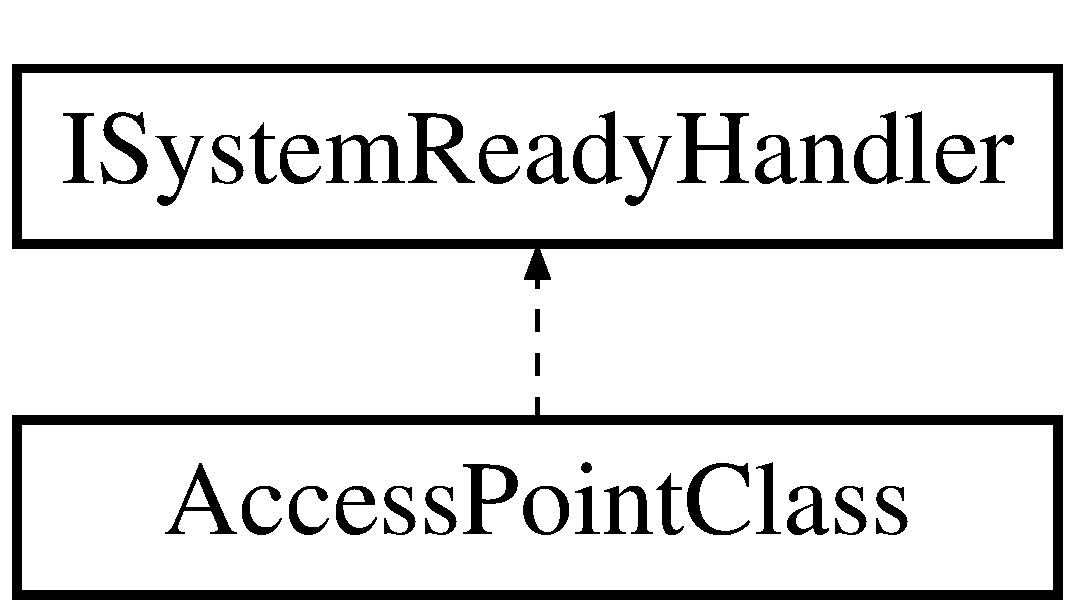
\includegraphics[height=2.000000cm]{class_access_point_class}
\end{center}
\end{figure}
\subsection*{Public Member Functions}
\begin{DoxyCompactItemize}
\item 
\hypertarget{class_access_point_class_ae60f0c85e16ed930ed367b17dc5e573d}{}void {\bfseries enable} (bool enabled)\label{class_access_point_class_ae60f0c85e16ed930ed367b17dc5e573d}

\item 
\hypertarget{class_access_point_class_a305464a28372cfd2bfea6993b19ceb7f}{}bool {\bfseries is\+Enabled} ()\label{class_access_point_class_a305464a28372cfd2bfea6993b19ceb7f}

\item 
\hypertarget{class_access_point_class_a68aaa05943f9895d3cd5d4074e6354d4}{}bool {\bfseries config} (String ssid, String password, A\+U\+T\+H\+\_\+\+M\+O\+D\+E mode, bool hidden=false, int channel=7, int beacon\+Interval=200)\label{class_access_point_class_a68aaa05943f9895d3cd5d4074e6354d4}

\item 
\hypertarget{class_access_point_class_a2160f04e7d844b04a3eec1ed64d47f06}{}void {\bfseries disconnect} ()\label{class_access_point_class_a2160f04e7d844b04a3eec1ed64d47f06}

\item 
\hypertarget{class_access_point_class_a86061e944d41587d5b5355c45cc3b95f}{}\hyperlink{class_i_p_address}{I\+P\+Address} {\bfseries get\+I\+P} ()\label{class_access_point_class_a86061e944d41587d5b5355c45cc3b95f}

\item 
\hypertarget{class_access_point_class_a5fcd3f84c68fcaada0a548055c45b3cb}{}bool {\bfseries set\+I\+P} (\hyperlink{class_i_p_address}{I\+P\+Address} address)\label{class_access_point_class_a5fcd3f84c68fcaada0a548055c45b3cb}

\item 
\hypertarget{class_access_point_class_a9a6e9d50aa7c0b2349acf7bf986d237e}{}String {\bfseries get\+M\+A\+C} ()\label{class_access_point_class_a9a6e9d50aa7c0b2349acf7bf986d237e}

\end{DoxyCompactItemize}
\subsection*{Protected Member Functions}
\begin{DoxyCompactItemize}
\item 
\hypertarget{class_access_point_class_a3f1aa322373e757d6cd4b0d04724d091}{}virtual void {\bfseries on\+System\+Ready} ()\label{class_access_point_class_a3f1aa322373e757d6cd4b0d04724d091}

\end{DoxyCompactItemize}


The documentation for this class was generated from the following files\+:\begin{DoxyCompactItemize}
\item 
Sming\+Core/\+Platform/Access\+Point.\+h\item 
Sming\+Core/\+Platform/Access\+Point.\+cpp\end{DoxyCompactItemize}

\hypertarget{class_adafruit___g_f_x}{}\section{Adafruit\+\_\+\+G\+F\+X Class Reference}
\label{class_adafruit___g_f_x}\index{Adafruit\+\_\+\+G\+F\+X@{Adafruit\+\_\+\+G\+F\+X}}
Inheritance diagram for Adafruit\+\_\+\+G\+F\+X\+:\begin{figure}[H]
\begin{center}
\leavevmode
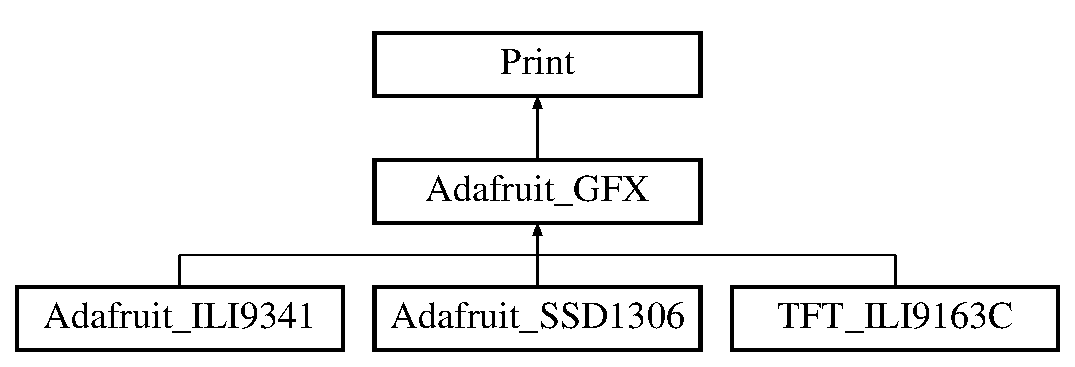
\includegraphics[height=3.000000cm]{class_adafruit___g_f_x}
\end{center}
\end{figure}
\subsection*{Public Member Functions}
\begin{DoxyCompactItemize}
\item 
\hypertarget{class_adafruit___g_f_x_a6f6f1abccf677eac244fa17d105133ea}{}{\bfseries Adafruit\+\_\+\+G\+F\+X} (int16\+\_\+t w, int16\+\_\+t h)\label{class_adafruit___g_f_x_a6f6f1abccf677eac244fa17d105133ea}

\item 
\hypertarget{class_adafruit___g_f_x_ab7fbf72885c873266f9c7eb53b5c8896}{}virtual void {\bfseries draw\+Pixel} (int16\+\_\+t x, int16\+\_\+t y, uint16\+\_\+t color)=0\label{class_adafruit___g_f_x_ab7fbf72885c873266f9c7eb53b5c8896}

\item 
\hypertarget{class_adafruit___g_f_x_aa0ff662c2b2b48c3bac51f98c777776d}{}virtual void {\bfseries draw\+Line} (int16\+\_\+t x0, int16\+\_\+t y0, int16\+\_\+t x1, int16\+\_\+t y1, uint16\+\_\+t color)\label{class_adafruit___g_f_x_aa0ff662c2b2b48c3bac51f98c777776d}

\item 
\hypertarget{class_adafruit___g_f_x_a1cffbb1d69c5faf49cd0cff27686a837}{}virtual void {\bfseries draw\+Fast\+V\+Line} (int16\+\_\+t x, int16\+\_\+t y, int16\+\_\+t h, uint16\+\_\+t color)\label{class_adafruit___g_f_x_a1cffbb1d69c5faf49cd0cff27686a837}

\item 
\hypertarget{class_adafruit___g_f_x_a4d42e7cc577c1eb5b06fe656786c9c79}{}virtual void {\bfseries draw\+Fast\+H\+Line} (int16\+\_\+t x, int16\+\_\+t y, int16\+\_\+t w, uint16\+\_\+t color)\label{class_adafruit___g_f_x_a4d42e7cc577c1eb5b06fe656786c9c79}

\item 
\hypertarget{class_adafruit___g_f_x_a9ec2c2ab426503e4f7deddb93bb916f6}{}virtual void {\bfseries draw\+Rect} (int16\+\_\+t x, int16\+\_\+t y, int16\+\_\+t w, int16\+\_\+t h, uint16\+\_\+t color)\label{class_adafruit___g_f_x_a9ec2c2ab426503e4f7deddb93bb916f6}

\item 
\hypertarget{class_adafruit___g_f_x_aa43cf1dfe6c17d040a0f1fd5ffbe9d69}{}virtual void {\bfseries fill\+Rect} (int16\+\_\+t x, int16\+\_\+t y, int16\+\_\+t w, int16\+\_\+t h, uint16\+\_\+t color)\label{class_adafruit___g_f_x_aa43cf1dfe6c17d040a0f1fd5ffbe9d69}

\item 
\hypertarget{class_adafruit___g_f_x_a2b2730aaf2208990928f9c0f85558527}{}virtual void {\bfseries fill\+Screen} (uint16\+\_\+t color)\label{class_adafruit___g_f_x_a2b2730aaf2208990928f9c0f85558527}

\item 
\hypertarget{class_adafruit___g_f_x_a2fa315803f39a5e73b1841874daf0483}{}virtual void {\bfseries invert\+Display} (boolean i)\label{class_adafruit___g_f_x_a2fa315803f39a5e73b1841874daf0483}

\item 
\hypertarget{class_adafruit___g_f_x_a648d2d6765e488b4556e802167d885fb}{}void {\bfseries draw\+Circle} (int16\+\_\+t x0, int16\+\_\+t y0, int16\+\_\+t r, uint16\+\_\+t color)\label{class_adafruit___g_f_x_a648d2d6765e488b4556e802167d885fb}

\item 
\hypertarget{class_adafruit___g_f_x_a3f2dd7b698e7b95ebf9fecf992ff802e}{}void {\bfseries draw\+Circle\+Helper} (int16\+\_\+t x0, int16\+\_\+t y0, int16\+\_\+t r, uint8\+\_\+t cornername, uint16\+\_\+t color)\label{class_adafruit___g_f_x_a3f2dd7b698e7b95ebf9fecf992ff802e}

\item 
\hypertarget{class_adafruit___g_f_x_a623e031e58492fb41e9fde6a05d97c12}{}void {\bfseries fill\+Circle} (int16\+\_\+t x0, int16\+\_\+t y0, int16\+\_\+t r, uint16\+\_\+t color)\label{class_adafruit___g_f_x_a623e031e58492fb41e9fde6a05d97c12}

\item 
\hypertarget{class_adafruit___g_f_x_a2242d3560b08c6480084152b6660052a}{}void {\bfseries fill\+Circle\+Helper} (int16\+\_\+t x0, int16\+\_\+t y0, int16\+\_\+t r, uint8\+\_\+t cornername, int16\+\_\+t delta, uint16\+\_\+t color)\label{class_adafruit___g_f_x_a2242d3560b08c6480084152b6660052a}

\item 
\hypertarget{class_adafruit___g_f_x_a49284b9cea16ecf8c15dfd0b51a841e6}{}void {\bfseries draw\+Triangle} (int16\+\_\+t x0, int16\+\_\+t y0, int16\+\_\+t x1, int16\+\_\+t y1, int16\+\_\+t x2, int16\+\_\+t y2, uint16\+\_\+t color)\label{class_adafruit___g_f_x_a49284b9cea16ecf8c15dfd0b51a841e6}

\item 
\hypertarget{class_adafruit___g_f_x_a4cd646a3d9c9d5b3ee50010d0aa387cd}{}void {\bfseries fill\+Triangle} (int16\+\_\+t x0, int16\+\_\+t y0, int16\+\_\+t x1, int16\+\_\+t y1, int16\+\_\+t x2, int16\+\_\+t y2, uint16\+\_\+t color)\label{class_adafruit___g_f_x_a4cd646a3d9c9d5b3ee50010d0aa387cd}

\item 
\hypertarget{class_adafruit___g_f_x_ab496b247abec724ef80e17a30257972b}{}void {\bfseries draw\+Round\+Rect} (int16\+\_\+t x0, int16\+\_\+t y0, int16\+\_\+t w, int16\+\_\+t h, int16\+\_\+t radius, uint16\+\_\+t color)\label{class_adafruit___g_f_x_ab496b247abec724ef80e17a30257972b}

\item 
\hypertarget{class_adafruit___g_f_x_a78dc59f6a508bcd3d5ac7af957b8b1ac}{}void {\bfseries fill\+Round\+Rect} (int16\+\_\+t x0, int16\+\_\+t y0, int16\+\_\+t w, int16\+\_\+t h, int16\+\_\+t radius, uint16\+\_\+t color)\label{class_adafruit___g_f_x_a78dc59f6a508bcd3d5ac7af957b8b1ac}

\item 
\hypertarget{class_adafruit___g_f_x_a50bf54503493152eeefa36f9768acec2}{}void {\bfseries draw\+Bitmap} (int16\+\_\+t x, int16\+\_\+t y, const uint8\+\_\+t $\ast$bitmap, int16\+\_\+t w, int16\+\_\+t h, uint16\+\_\+t color)\label{class_adafruit___g_f_x_a50bf54503493152eeefa36f9768acec2}

\item 
\hypertarget{class_adafruit___g_f_x_a5225478b3f2afefcb16ed03e9fe93dc0}{}void {\bfseries draw\+Bitmap} (int16\+\_\+t x, int16\+\_\+t y, const uint8\+\_\+t $\ast$bitmap, int16\+\_\+t w, int16\+\_\+t h, uint16\+\_\+t color, uint16\+\_\+t bg)\label{class_adafruit___g_f_x_a5225478b3f2afefcb16ed03e9fe93dc0}

\item 
\hypertarget{class_adafruit___g_f_x_acec26bcf41c15ac6826c67e1f5e4cde6}{}void {\bfseries draw\+X\+Bitmap} (int16\+\_\+t x, int16\+\_\+t y, const uint8\+\_\+t $\ast$bitmap, int16\+\_\+t w, int16\+\_\+t h, uint16\+\_\+t color)\label{class_adafruit___g_f_x_acec26bcf41c15ac6826c67e1f5e4cde6}

\item 
\hypertarget{class_adafruit___g_f_x_ab7f5a29b3a3dffe30c6a3f4c1f604a5a}{}void {\bfseries draw\+Char} (int16\+\_\+t x, int16\+\_\+t y, unsigned char c, uint16\+\_\+t color, uint16\+\_\+t bg, uint8\+\_\+t size)\label{class_adafruit___g_f_x_ab7f5a29b3a3dffe30c6a3f4c1f604a5a}

\item 
\hypertarget{class_adafruit___g_f_x_aaf96a40cad0f34dd8ec73494b3866c33}{}void {\bfseries set\+Cursor} (int16\+\_\+t x, int16\+\_\+t y)\label{class_adafruit___g_f_x_aaf96a40cad0f34dd8ec73494b3866c33}

\item 
\hypertarget{class_adafruit___g_f_x_a59178a0e0c845a14a39b457c43567dd9}{}void {\bfseries set\+Text\+Color} (uint16\+\_\+t c)\label{class_adafruit___g_f_x_a59178a0e0c845a14a39b457c43567dd9}

\item 
\hypertarget{class_adafruit___g_f_x_ab6e88c585d3ab6b4f95199361f224fc6}{}void {\bfseries set\+Text\+Color} (uint16\+\_\+t c, uint16\+\_\+t bg)\label{class_adafruit___g_f_x_ab6e88c585d3ab6b4f95199361f224fc6}

\item 
\hypertarget{class_adafruit___g_f_x_a39eb4a8a2c9fa4ab7d58ceffd19535d5}{}void {\bfseries set\+Text\+Size} (uint8\+\_\+t s)\label{class_adafruit___g_f_x_a39eb4a8a2c9fa4ab7d58ceffd19535d5}

\item 
\hypertarget{class_adafruit___g_f_x_aeeacd62bf26f3e7abbdc4b5b50faa6fa}{}void {\bfseries set\+Text\+Wrap} (boolean w)\label{class_adafruit___g_f_x_aeeacd62bf26f3e7abbdc4b5b50faa6fa}

\item 
\hypertarget{class_adafruit___g_f_x_a6ac337c49876cee23ed062a928724675}{}void {\bfseries set\+Rotation} (uint8\+\_\+t r)\label{class_adafruit___g_f_x_a6ac337c49876cee23ed062a928724675}

\item 
\hypertarget{class_adafruit___g_f_x_af4978ea0cf0c0b0540567e82d8fa9900}{}virtual void {\bfseries write} (uint8\+\_\+t)\label{class_adafruit___g_f_x_af4978ea0cf0c0b0540567e82d8fa9900}

\item 
\hypertarget{class_adafruit___g_f_x_ac3dea6208d543a50f89b8e81bcaf9f09}{}int16\+\_\+t {\bfseries height} (void) const \label{class_adafruit___g_f_x_ac3dea6208d543a50f89b8e81bcaf9f09}

\item 
\hypertarget{class_adafruit___g_f_x_a32dadc6651cedc5e6426322c8a922cd6}{}int16\+\_\+t {\bfseries width} (void) const \label{class_adafruit___g_f_x_a32dadc6651cedc5e6426322c8a922cd6}

\item 
\hypertarget{class_adafruit___g_f_x_a1956ad03632c73f25b4d8d240a40d7c9}{}uint8\+\_\+t {\bfseries get\+Rotation} (void) const \label{class_adafruit___g_f_x_a1956ad03632c73f25b4d8d240a40d7c9}

\end{DoxyCompactItemize}
\subsection*{Protected Attributes}
\begin{DoxyCompactItemize}
\item 
\hypertarget{class_adafruit___g_f_x_ab693a8ac5d94c50c2558b5a3795ddde4}{}const int16\+\_\+t {\bfseries W\+I\+D\+T\+H}\label{class_adafruit___g_f_x_ab693a8ac5d94c50c2558b5a3795ddde4}

\item 
\hypertarget{class_adafruit___g_f_x_a6b3665babcb73df381563016e9f71bdb}{}const int16\+\_\+t {\bfseries H\+E\+I\+G\+H\+T}\label{class_adafruit___g_f_x_a6b3665babcb73df381563016e9f71bdb}

\item 
\hypertarget{class_adafruit___g_f_x_ab237f850a033492f5e745d79405a097a}{}int16\+\_\+t {\bfseries \+\_\+width}\label{class_adafruit___g_f_x_ab237f850a033492f5e745d79405a097a}

\item 
\hypertarget{class_adafruit___g_f_x_ab9bb0cbc2455f64dce2a5ec36307aa94}{}int16\+\_\+t {\bfseries \+\_\+height}\label{class_adafruit___g_f_x_ab9bb0cbc2455f64dce2a5ec36307aa94}

\item 
\hypertarget{class_adafruit___g_f_x_a8f8983cea8d81a7c8e9d05eef36318e2}{}int16\+\_\+t {\bfseries cursor\+\_\+x}\label{class_adafruit___g_f_x_a8f8983cea8d81a7c8e9d05eef36318e2}

\item 
\hypertarget{class_adafruit___g_f_x_aebe0a38f6e6fd59cb81620c4696286c9}{}int16\+\_\+t {\bfseries cursor\+\_\+y}\label{class_adafruit___g_f_x_aebe0a38f6e6fd59cb81620c4696286c9}

\item 
\hypertarget{class_adafruit___g_f_x_a8c6d23a386651136fd9530a5b7046591}{}uint16\+\_\+t {\bfseries textcolor}\label{class_adafruit___g_f_x_a8c6d23a386651136fd9530a5b7046591}

\item 
\hypertarget{class_adafruit___g_f_x_a23e7a4efcab0b1588dc0cafa14b1fac1}{}uint16\+\_\+t {\bfseries textbgcolor}\label{class_adafruit___g_f_x_a23e7a4efcab0b1588dc0cafa14b1fac1}

\item 
\hypertarget{class_adafruit___g_f_x_ac293848b8fe8c46107d1a491f6a5168d}{}uint8\+\_\+t {\bfseries textsize}\label{class_adafruit___g_f_x_ac293848b8fe8c46107d1a491f6a5168d}

\item 
\hypertarget{class_adafruit___g_f_x_a37a479d28fb11906ce516e983b1af926}{}uint8\+\_\+t {\bfseries rotation}\label{class_adafruit___g_f_x_a37a479d28fb11906ce516e983b1af926}

\item 
\hypertarget{class_adafruit___g_f_x_ad6bd603e01861212829d536312a7190b}{}boolean {\bfseries wrap}\label{class_adafruit___g_f_x_ad6bd603e01861212829d536312a7190b}

\end{DoxyCompactItemize}


The documentation for this class was generated from the following files\+:\begin{DoxyCompactItemize}
\item 
Libraries/\+Adafruit\+\_\+\+G\+F\+X/Adafruit\+\_\+\+G\+F\+X.\+h\item 
Libraries/\+Adafruit\+\_\+\+G\+F\+X/Adafruit\+\_\+\+G\+F\+X.\+cpp\end{DoxyCompactItemize}

\hypertarget{class_adafruit___i_l_i9341}{}\section{Adafruit\+\_\+\+I\+L\+I9341 Class Reference}
\label{class_adafruit___i_l_i9341}\index{Adafruit\+\_\+\+I\+L\+I9341@{Adafruit\+\_\+\+I\+L\+I9341}}
Inheritance diagram for Adafruit\+\_\+\+I\+L\+I9341\+:\begin{figure}[H]
\begin{center}
\leavevmode
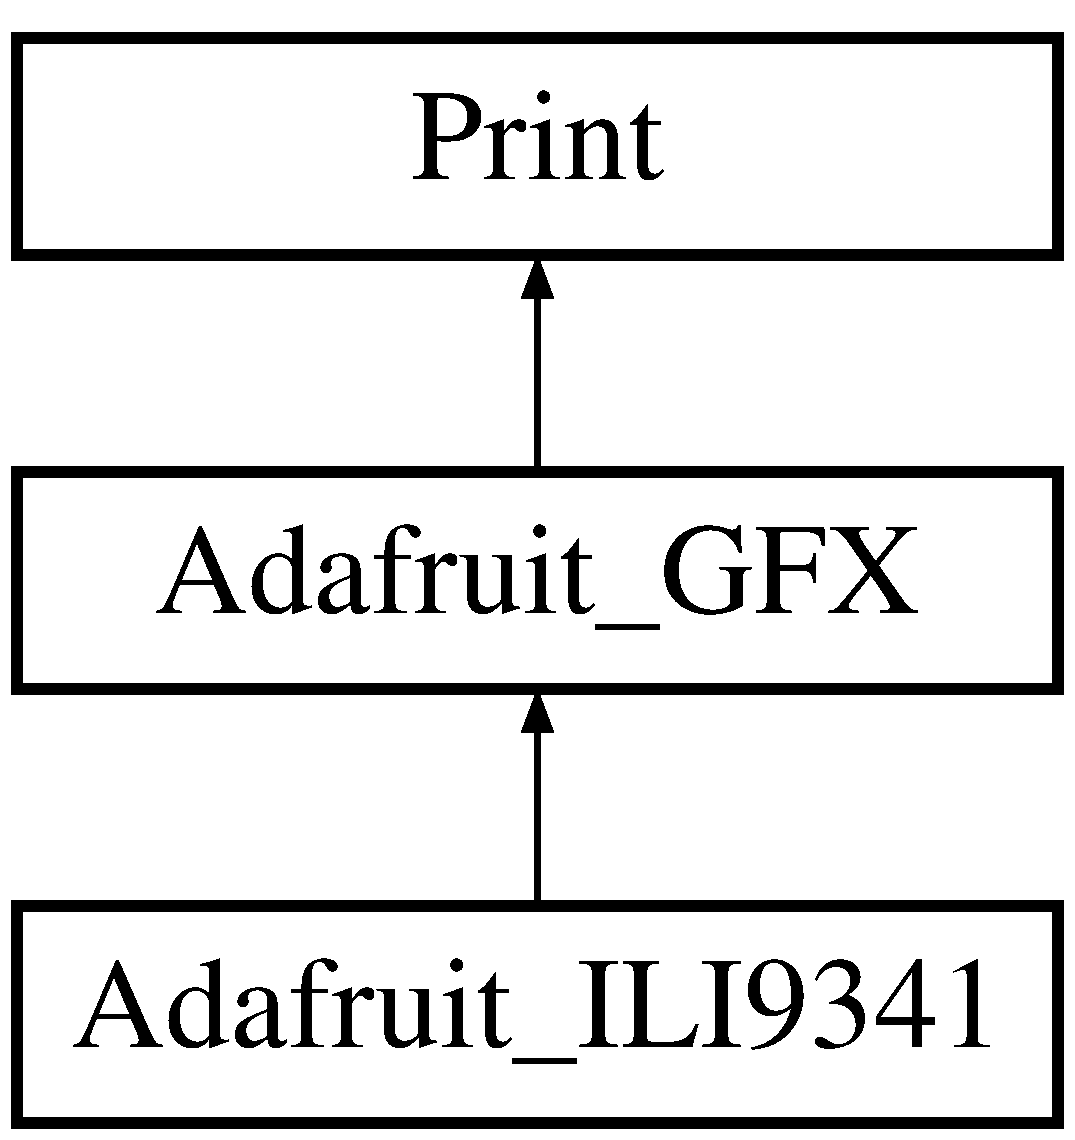
\includegraphics[height=3.000000cm]{class_adafruit___i_l_i9341}
\end{center}
\end{figure}
\subsection*{Public Member Functions}
\begin{DoxyCompactItemize}
\item 
\hypertarget{class_adafruit___i_l_i9341_ac888d6593f1e3bad4d2b22b4e159616e}{}void {\bfseries begin} (void)\label{class_adafruit___i_l_i9341_ac888d6593f1e3bad4d2b22b4e159616e}

\item 
\hypertarget{class_adafruit___i_l_i9341_a8ddbebf26c29ac4ae9dcba5f245bcf22}{}void {\bfseries fill\+Screen} (uint16\+\_\+t color)\label{class_adafruit___i_l_i9341_a8ddbebf26c29ac4ae9dcba5f245bcf22}

\item 
\hypertarget{class_adafruit___i_l_i9341_a05e026d2694e464ec40ea4c41b2156a3}{}void {\bfseries draw\+Pixel} (int16\+\_\+t x, int16\+\_\+t y, uint16\+\_\+t color)\label{class_adafruit___i_l_i9341_a05e026d2694e464ec40ea4c41b2156a3}

\item 
\hypertarget{class_adafruit___i_l_i9341_abad7dca69da48516407451326210b89b}{}void {\bfseries draw\+Fast\+V\+Line} (int16\+\_\+t x, int16\+\_\+t y, int16\+\_\+t h, uint16\+\_\+t color)\label{class_adafruit___i_l_i9341_abad7dca69da48516407451326210b89b}

\item 
\hypertarget{class_adafruit___i_l_i9341_a183d65bf81c6e6b02daa256cf85cd875}{}void {\bfseries draw\+Fast\+H\+Line} (int16\+\_\+t x, int16\+\_\+t y, int16\+\_\+t w, uint16\+\_\+t color)\label{class_adafruit___i_l_i9341_a183d65bf81c6e6b02daa256cf85cd875}

\item 
\hypertarget{class_adafruit___i_l_i9341_ac9dad828fc0ac895ec857c83d79da5eb}{}void {\bfseries fill\+Rect} (int16\+\_\+t x, int16\+\_\+t y, int16\+\_\+t w, int16\+\_\+t h, uint16\+\_\+t color)\label{class_adafruit___i_l_i9341_ac9dad828fc0ac895ec857c83d79da5eb}

\item 
\hypertarget{class_adafruit___i_l_i9341_ae82ff4003dba45826284ff16791a647c}{}void {\bfseries set\+Rotation} (uint8\+\_\+t r)\label{class_adafruit___i_l_i9341_ae82ff4003dba45826284ff16791a647c}

\item 
\hypertarget{class_adafruit___i_l_i9341_aeebe7e19bba4eea54f72223af0b580c2}{}void {\bfseries invert\+Display} (bool i)\label{class_adafruit___i_l_i9341_aeebe7e19bba4eea54f72223af0b580c2}

\item 
\hypertarget{class_adafruit___i_l_i9341_a5f8856f69cf45a14b4500e58a3322470}{}void {\bfseries set\+Addr\+Window} (uint16\+\_\+t x0, uint16\+\_\+t y0, uint16\+\_\+t x1, uint16\+\_\+t y1)\label{class_adafruit___i_l_i9341_a5f8856f69cf45a14b4500e58a3322470}

\item 
\hypertarget{class_adafruit___i_l_i9341_a3ae835b461eedc7cfd687110ff5cb447}{}uint16\+\_\+t {\bfseries color565} (uint8\+\_\+t r, uint8\+\_\+t g, uint8\+\_\+t b)\label{class_adafruit___i_l_i9341_a3ae835b461eedc7cfd687110ff5cb447}

\end{DoxyCompactItemize}
\subsection*{Additional Inherited Members}


The documentation for this class was generated from the following files\+:\begin{DoxyCompactItemize}
\item 
Libraries/\+Adafruit\+\_\+\+I\+L\+I9341/Adafruit\+\_\+\+I\+L\+I9341.\+h\item 
Libraries/\+Adafruit\+\_\+\+I\+L\+I9341/Adafruit\+\_\+\+I\+L\+I9341.\+cpp\end{DoxyCompactItemize}

\hypertarget{class_adafruit___s_s_d1306}{}\section{Adafruit\+\_\+\+S\+S\+D1306 Class Reference}
\label{class_adafruit___s_s_d1306}\index{Adafruit\+\_\+\+S\+S\+D1306@{Adafruit\+\_\+\+S\+S\+D1306}}
Inheritance diagram for Adafruit\+\_\+\+S\+S\+D1306\+:\begin{figure}[H]
\begin{center}
\leavevmode
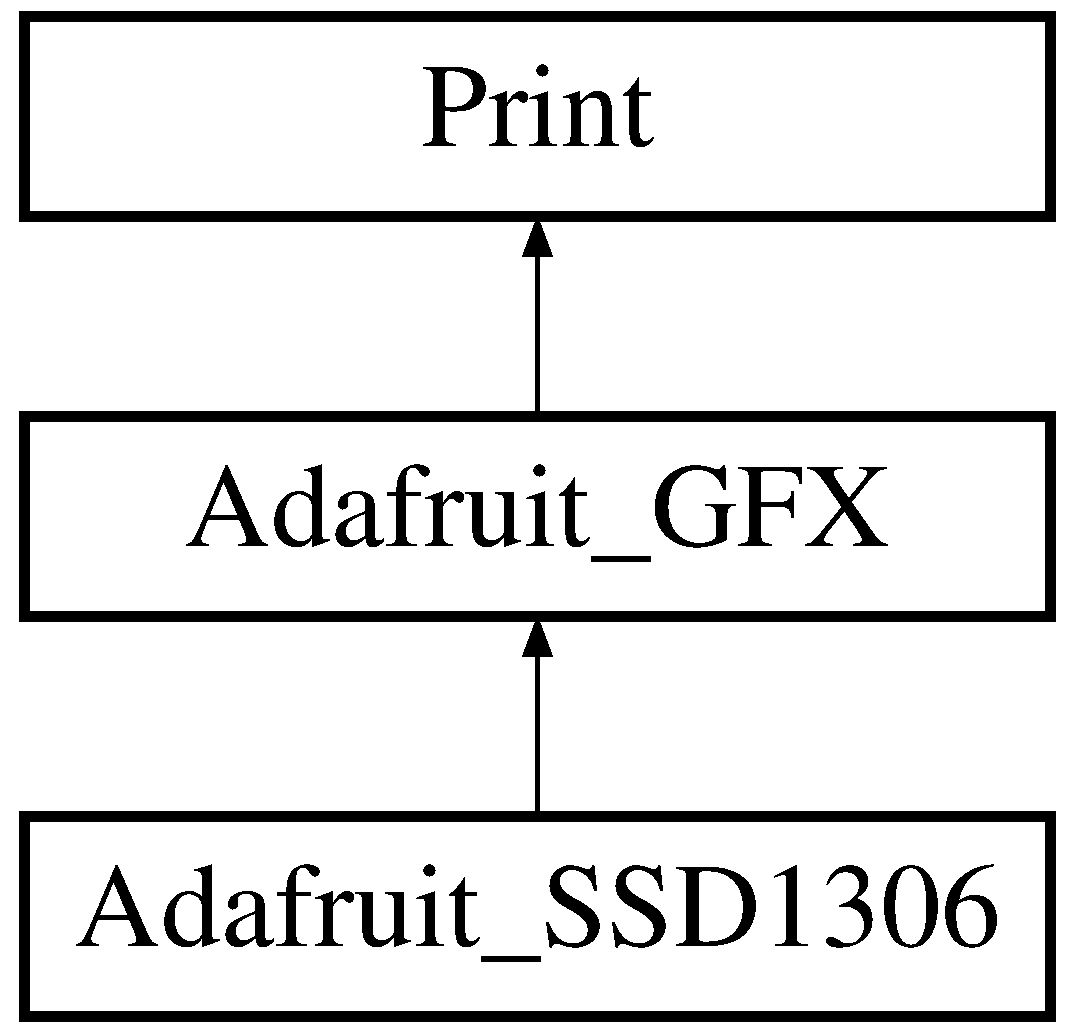
\includegraphics[height=3.000000cm]{class_adafruit___s_s_d1306}
\end{center}
\end{figure}
\subsection*{Public Member Functions}
\begin{DoxyCompactItemize}
\item 
\hypertarget{class_adafruit___s_s_d1306_afa528a297f64684f6b81d2918fee76ea}{}{\bfseries Adafruit\+\_\+\+S\+S\+D1306} (int8\+\_\+t S\+I\+D, int8\+\_\+t S\+C\+L\+K, int8\+\_\+t D\+C, int8\+\_\+t R\+S\+T, int8\+\_\+t C\+S)\label{class_adafruit___s_s_d1306_afa528a297f64684f6b81d2918fee76ea}

\item 
\hypertarget{class_adafruit___s_s_d1306_aa7fcad43307cfed089bf7f4a7ce5ffbc}{}{\bfseries Adafruit\+\_\+\+S\+S\+D1306} (int8\+\_\+t D\+C, int8\+\_\+t R\+S\+T, int8\+\_\+t C\+S)\label{class_adafruit___s_s_d1306_aa7fcad43307cfed089bf7f4a7ce5ffbc}

\item 
\hypertarget{class_adafruit___s_s_d1306_aac7f93129e1d0f1a151f926ebc23643d}{}{\bfseries Adafruit\+\_\+\+S\+S\+D1306} (int8\+\_\+t R\+S\+T)\label{class_adafruit___s_s_d1306_aac7f93129e1d0f1a151f926ebc23643d}

\item 
\hypertarget{class_adafruit___s_s_d1306_a804a4689c2e09a5300f72251fd481a1b}{}void {\bfseries begin} (uint8\+\_\+t switchvcc=S\+S\+D1306\+\_\+\+S\+W\+I\+T\+C\+H\+C\+A\+P\+V\+C\+C, uint8\+\_\+t i2caddr=S\+S\+D1306\+\_\+\+I2\+C\+\_\+\+A\+D\+D\+R\+E\+S\+S, bool reset=true)\label{class_adafruit___s_s_d1306_a804a4689c2e09a5300f72251fd481a1b}

\item 
\hypertarget{class_adafruit___s_s_d1306_a99182555a08549492f6c40ceea0abc3d}{}void {\bfseries ssd1306\+\_\+command} (uint8\+\_\+t c)\label{class_adafruit___s_s_d1306_a99182555a08549492f6c40ceea0abc3d}

\item 
\hypertarget{class_adafruit___s_s_d1306_a694dc2e0d8e07ac144742119a4f55cfe}{}void {\bfseries ssd1306\+\_\+data} (uint8\+\_\+t c)\label{class_adafruit___s_s_d1306_a694dc2e0d8e07ac144742119a4f55cfe}

\item 
\hypertarget{class_adafruit___s_s_d1306_afe1e0f5efabd931aab7998275356744d}{}void {\bfseries clear\+Display} (void)\label{class_adafruit___s_s_d1306_afe1e0f5efabd931aab7998275356744d}

\item 
\hypertarget{class_adafruit___s_s_d1306_aff04df12e2ec8b6a57a9b9856b507cf4}{}void {\bfseries invert\+Display} (uint8\+\_\+t i)\label{class_adafruit___s_s_d1306_aff04df12e2ec8b6a57a9b9856b507cf4}

\item 
\hypertarget{class_adafruit___s_s_d1306_aeaa87aea232bb42cbcc642e510f0d95a}{}void {\bfseries display} ()\label{class_adafruit___s_s_d1306_aeaa87aea232bb42cbcc642e510f0d95a}

\item 
\hypertarget{class_adafruit___s_s_d1306_a6a9f18f43c19296dc54dfb657eab4d66}{}void {\bfseries startscrollright} (uint8\+\_\+t start, uint8\+\_\+t stop)\label{class_adafruit___s_s_d1306_a6a9f18f43c19296dc54dfb657eab4d66}

\item 
\hypertarget{class_adafruit___s_s_d1306_a4c58c2a4ac905e199d6ced49a0098296}{}void {\bfseries startscrollleft} (uint8\+\_\+t start, uint8\+\_\+t stop)\label{class_adafruit___s_s_d1306_a4c58c2a4ac905e199d6ced49a0098296}

\item 
\hypertarget{class_adafruit___s_s_d1306_adbc9f95bb91eb0e76c4465d3c4d941e1}{}void {\bfseries startscrolldiagright} (uint8\+\_\+t start, uint8\+\_\+t stop)\label{class_adafruit___s_s_d1306_adbc9f95bb91eb0e76c4465d3c4d941e1}

\item 
\hypertarget{class_adafruit___s_s_d1306_a8d5b19419f508e5133053fa39da10f98}{}void {\bfseries startscrolldiagleft} (uint8\+\_\+t start, uint8\+\_\+t stop)\label{class_adafruit___s_s_d1306_a8d5b19419f508e5133053fa39da10f98}

\item 
\hypertarget{class_adafruit___s_s_d1306_ab4559d6aae71a4de8969f9160a6eda40}{}void {\bfseries stopscroll} (void)\label{class_adafruit___s_s_d1306_ab4559d6aae71a4de8969f9160a6eda40}

\item 
\hypertarget{class_adafruit___s_s_d1306_ae918422325b9fabc7396207263269d3a}{}void {\bfseries dim} (boolean dim)\label{class_adafruit___s_s_d1306_ae918422325b9fabc7396207263269d3a}

\item 
\hypertarget{class_adafruit___s_s_d1306_ae2851d927a047a770c569c7c9fde4807}{}void {\bfseries draw\+Pixel} (int16\+\_\+t x, int16\+\_\+t y, uint16\+\_\+t color)\label{class_adafruit___s_s_d1306_ae2851d927a047a770c569c7c9fde4807}

\item 
\hypertarget{class_adafruit___s_s_d1306_a2058c782206fd0c7a74a1d6d19a383b6}{}virtual void {\bfseries draw\+Fast\+V\+Line} (int16\+\_\+t x, int16\+\_\+t y, int16\+\_\+t h, uint16\+\_\+t color)\label{class_adafruit___s_s_d1306_a2058c782206fd0c7a74a1d6d19a383b6}

\item 
\hypertarget{class_adafruit___s_s_d1306_a8165eca9ccfee431af10b6f5fa06a406}{}virtual void {\bfseries draw\+Fast\+H\+Line} (int16\+\_\+t x, int16\+\_\+t y, int16\+\_\+t w, uint16\+\_\+t color)\label{class_adafruit___s_s_d1306_a8165eca9ccfee431af10b6f5fa06a406}

\end{DoxyCompactItemize}
\subsection*{Additional Inherited Members}


The documentation for this class was generated from the following files\+:\begin{DoxyCompactItemize}
\item 
Libraries/\+Adafruit\+\_\+\+S\+S\+D1306/Adafruit\+\_\+\+S\+S\+D1306.\+h\item 
Libraries/\+Adafruit\+\_\+\+S\+S\+D1306/Adafruit\+\_\+\+S\+S\+D1306.\+cpp\end{DoxyCompactItemize}

\hypertarget{class_b_h1750_f_v_i}{}\section{B\+H1750\+F\+V\+I Class Reference}
\label{class_b_h1750_f_v_i}\index{B\+H1750\+F\+V\+I@{B\+H1750\+F\+V\+I}}
\subsection*{Public Member Functions}
\begin{DoxyCompactItemize}
\item 
\hypertarget{class_b_h1750_f_v_i_a87363c13729aee32e28c7e710bdcecf3}{}{\bfseries B\+H1750\+F\+V\+I} (byte address)\label{class_b_h1750_f_v_i_a87363c13729aee32e28c7e710bdcecf3}

\item 
\hypertarget{class_b_h1750_f_v_i_a1b18d85ef3ffcd34c63beb2062061f70}{}bool {\bfseries begin} (void)\label{class_b_h1750_f_v_i_a1b18d85ef3ffcd34c63beb2062061f70}

\item 
\hypertarget{class_b_h1750_f_v_i_a4fa874233e7f977a52e7279557ef1245}{}void {\bfseries sleep} (void)\label{class_b_h1750_f_v_i_a4fa874233e7f977a52e7279557ef1245}

\item 
\hypertarget{class_b_h1750_f_v_i_a33d2b3774837fd7375302d154f851efc}{}void {\bfseries set\+Mode} (uint8\+\_\+t M\+O\+D\+E)\label{class_b_h1750_f_v_i_a33d2b3774837fd7375302d154f851efc}

\item 
\hypertarget{class_b_h1750_f_v_i_a3ce11aec23163613f83ac76de9b5872b}{}void {\bfseries reset} (void)\label{class_b_h1750_f_v_i_a3ce11aec23163613f83ac76de9b5872b}

\item 
\hypertarget{class_b_h1750_f_v_i_a7ee84f4b34a92091a37790fea3c72070}{}uint16\+\_\+t {\bfseries get\+Light\+Intensity} (void)\label{class_b_h1750_f_v_i_a7ee84f4b34a92091a37790fea3c72070}

\end{DoxyCompactItemize}


The documentation for this class was generated from the following files\+:\begin{DoxyCompactItemize}
\item 
Libraries/\+B\+H1750\+F\+V\+I/B\+H1750\+F\+V\+I.\+h\item 
Libraries/\+B\+H1750\+F\+V\+I/B\+H1750\+F\+V\+I.\+cpp\end{DoxyCompactItemize}

\hypertarget{class_b_m_p180}{}\section{B\+M\+P180 Class Reference}
\label{class_b_m_p180}\index{B\+M\+P180@{B\+M\+P180}}
\subsection*{Public Member Functions}
\begin{DoxyCompactItemize}
\item 
\hypertarget{class_b_m_p180_aa0d204ff14f242e7dae7f17616f384b5}{}void {\bfseries Initialize} (void)\label{class_b_m_p180_aa0d204ff14f242e7dae7f17616f384b5}

\item 
\hypertarget{class_b_m_p180_a25efcc78a47f50bb416252dd6589c5b2}{}int {\bfseries Get\+Uncompensated\+Temperature} ()\label{class_b_m_p180_a25efcc78a47f50bb416252dd6589c5b2}

\item 
\hypertarget{class_b_m_p180_aaa9d85bd4b3e01ed5f8145672ebd11b0}{}float {\bfseries Compensate\+Temperature} (int uncompensated\+Temperature)\label{class_b_m_p180_aaa9d85bd4b3e01ed5f8145672ebd11b0}

\item 
\hypertarget{class_b_m_p180_aeffb6785b31ee9cc4c22e66341d61985}{}long {\bfseries Get\+Uncompensated\+Pressure} ()\label{class_b_m_p180_aeffb6785b31ee9cc4c22e66341d61985}

\item 
\hypertarget{class_b_m_p180_a0a6ea646db93f926d7883f2c48d69f90}{}long {\bfseries Compensate\+Pressure} (long uncompensated\+Pressure)\label{class_b_m_p180_a0a6ea646db93f926d7883f2c48d69f90}

\item 
\hypertarget{class_b_m_p180_a57b06b78699af8789354f0a3788d540a}{}float {\bfseries Get\+Temperature} ()\label{class_b_m_p180_a57b06b78699af8789354f0a3788d540a}

\item 
\hypertarget{class_b_m_p180_a332e20330d5a0a82b7a92c928b828651}{}long {\bfseries Get\+Pressure} ()\label{class_b_m_p180_a332e20330d5a0a82b7a92c928b828651}

\item 
\hypertarget{class_b_m_p180_af0b57d651f198db167085a3728f9b2a8}{}void {\bfseries Soft\+Reset} ()\label{class_b_m_p180_af0b57d651f198db167085a3728f9b2a8}

\item 
\hypertarget{class_b_m_p180_aa70a022147dac9c4c70a69e5412c057d}{}uint8\+\_\+t {\bfseries Set\+Resolution} (uint8\+\_\+t sample\+Resolution, bool oversample)\label{class_b_m_p180_aa70a022147dac9c4c70a69e5412c057d}

\item 
\hypertarget{class_b_m_p180_a1739c26c21737920771532e5cd5c4d3d}{}void {\bfseries Print\+Calibration\+Data} ()\label{class_b_m_p180_a1739c26c21737920771532e5cd5c4d3d}

\item 
\hypertarget{class_b_m_p180_ab8ef034f33153809afb15c1b4df1387a}{}uint8\+\_\+t {\bfseries Ensure\+Connected} ()\label{class_b_m_p180_ab8ef034f33153809afb15c1b4df1387a}

\item 
\hypertarget{class_b_m_p180_ace5e813b9936ef2075d6f088b9ceeabf}{}const char $\ast$ {\bfseries Get\+Error\+Text} (int error\+Code)\label{class_b_m_p180_ace5e813b9936ef2075d6f088b9ceeabf}

\end{DoxyCompactItemize}
\subsection*{Public Attributes}
\begin{DoxyCompactItemize}
\item 
\hypertarget{class_b_m_p180_a7fe61f0655d615011abdf84431145a95}{}uint8\+\_\+t {\bfseries Is\+Connected}\label{class_b_m_p180_a7fe61f0655d615011abdf84431145a95}

\end{DoxyCompactItemize}
\subsection*{Protected Member Functions}
\begin{DoxyCompactItemize}
\item 
\hypertarget{class_b_m_p180_a4282e16c218dcbd6c1f4e45adad47874}{}void {\bfseries Write} (int address, int byte)\label{class_b_m_p180_a4282e16c218dcbd6c1f4e45adad47874}

\item 
\hypertarget{class_b_m_p180_a66dc9d1ba888abe9389248c5b1d0b418}{}uint8\+\_\+t $\ast$ {\bfseries Read} (int address, int length)\label{class_b_m_p180_a66dc9d1ba888abe9389248c5b1d0b418}

\item 
\hypertarget{class_b_m_p180_a20c19a359b882a25495b21bcbfb5f6f3}{}void {\bfseries Read2} (int address, int length, uint8\+\_\+t buffer\mbox{[}$\,$\mbox{]})\label{class_b_m_p180_a20c19a359b882a25495b21bcbfb5f6f3}

\end{DoxyCompactItemize}


The documentation for this class was generated from the following files\+:\begin{DoxyCompactItemize}
\item 
Libraries/\+B\+M\+P180/B\+M\+P180.\+h\item 
Libraries/\+B\+M\+P180/B\+M\+P180.\+cpp\end{DoxyCompactItemize}

\hypertarget{class_bounce}{}\section{Bounce Class Reference}
\label{class_bounce}\index{Bounce@{Bounce}}
\subsection*{Public Member Functions}
\begin{DoxyCompactItemize}
\item 
\hypertarget{class_bounce_ab34517094faf21d4f38b36da2915132b}{}{\bfseries Bounce} (uint8\+\_\+t pin, unsigned long interval\+\_\+millis)\label{class_bounce_ab34517094faf21d4f38b36da2915132b}

\item 
\hypertarget{class_bounce_a952fd33da52d169784b4bac37846c808}{}void {\bfseries interval} (unsigned long interval\+\_\+millis)\label{class_bounce_a952fd33da52d169784b4bac37846c808}

\item 
\hypertarget{class_bounce_a5044403b77e2751adc13fffe984b8b65}{}int {\bfseries update} ()\label{class_bounce_a5044403b77e2751adc13fffe984b8b65}

\item 
\hypertarget{class_bounce_add7fe88ebe6b8bbcc7528701d2914457}{}void {\bfseries rebounce} (unsigned long interval)\label{class_bounce_add7fe88ebe6b8bbcc7528701d2914457}

\item 
\hypertarget{class_bounce_ae50a234cdadfac51ef8ebc6011b1c702}{}int {\bfseries read} ()\label{class_bounce_ae50a234cdadfac51ef8ebc6011b1c702}

\item 
\hypertarget{class_bounce_a4f51731e4c1c5c73a522056ccb87d5d0}{}void {\bfseries write} (int new\+\_\+state)\label{class_bounce_a4f51731e4c1c5c73a522056ccb87d5d0}

\item 
\hypertarget{class_bounce_a62412d814d36102ab3d285e801d5d29a}{}unsigned long {\bfseries duration} ()\label{class_bounce_a62412d814d36102ab3d285e801d5d29a}

\item 
\hypertarget{class_bounce_a3417beb80eb6593d768c2e9884c57aa0}{}bool {\bfseries rising\+Edge} ()\label{class_bounce_a3417beb80eb6593d768c2e9884c57aa0}

\item 
\hypertarget{class_bounce_ac756559419bfa1c5060e5e4a4ad6406f}{}bool {\bfseries falling\+Edge} ()\label{class_bounce_ac756559419bfa1c5060e5e4a4ad6406f}

\end{DoxyCompactItemize}
\subsection*{Protected Member Functions}
\begin{DoxyCompactItemize}
\item 
\hypertarget{class_bounce_aee8349a42e798e59a2fea9c3dca53569}{}int {\bfseries debounce} ()\label{class_bounce_aee8349a42e798e59a2fea9c3dca53569}

\end{DoxyCompactItemize}
\subsection*{Protected Attributes}
\begin{DoxyCompactItemize}
\item 
\hypertarget{class_bounce_a223ab27b8094acd12d77a3a9145f56c9}{}unsigned long {\bfseries previous\+\_\+millis}\label{class_bounce_a223ab27b8094acd12d77a3a9145f56c9}

\item 
\hypertarget{class_bounce_a12f15211cdbc690e81a4a054183820bd}{}unsigned long {\bfseries interval\+\_\+millis}\label{class_bounce_a12f15211cdbc690e81a4a054183820bd}

\item 
\hypertarget{class_bounce_a6ddea36f65ef856546e3365af929ace6}{}unsigned long {\bfseries rebounce\+\_\+millis}\label{class_bounce_a6ddea36f65ef856546e3365af929ace6}

\item 
\hypertarget{class_bounce_af013db8b02e1e252eb60dd5b40d5480b}{}uint8\+\_\+t {\bfseries state}\label{class_bounce_af013db8b02e1e252eb60dd5b40d5480b}

\item 
\hypertarget{class_bounce_a1cb79cb0ba2379cd12cc7c098d97053a}{}uint8\+\_\+t {\bfseries pin}\label{class_bounce_a1cb79cb0ba2379cd12cc7c098d97053a}

\item 
\hypertarget{class_bounce_aee4ce3c901eaac62efc5d6bdb7beccdd}{}uint8\+\_\+t {\bfseries state\+Changed}\label{class_bounce_aee4ce3c901eaac62efc5d6bdb7beccdd}

\end{DoxyCompactItemize}


The documentation for this class was generated from the following files\+:\begin{DoxyCompactItemize}
\item 
Libraries/\+Bounce/Bounce.\+h\item 
Libraries/\+Bounce/Bounce.\+cpp\end{DoxyCompactItemize}

\hypertarget{class_bss_info}{}\section{Bss\+Info Class Reference}
\label{class_bss_info}\index{Bss\+Info@{Bss\+Info}}
\subsection*{Public Member Functions}
\begin{DoxyCompactItemize}
\item 
\hypertarget{class_bss_info_aec562770f28d1d9fcdd3b638ec0a6ecd}{}{\bfseries Bss\+Info} (bss\+\_\+info $\ast$info)\label{class_bss_info_aec562770f28d1d9fcdd3b638ec0a6ecd}

\item 
\hypertarget{class_bss_info_a0b7cfc6543a1057dc87bd83932dd6785}{}bool {\bfseries is\+Open} ()\label{class_bss_info_a0b7cfc6543a1057dc87bd83932dd6785}

\item 
\hypertarget{class_bss_info_aee47fe90704b37e0132ab3b845a30831}{}const char $\ast$ {\bfseries get\+Authorization\+Method\+Name} ()\label{class_bss_info_aee47fe90704b37e0132ab3b845a30831}

\item 
\hypertarget{class_bss_info_ad3f75400d8d164b64af11c995906bc7b}{}uint32\+\_\+t {\bfseries get\+Hash\+Id} ()\label{class_bss_info_ad3f75400d8d164b64af11c995906bc7b}

\end{DoxyCompactItemize}
\subsection*{Public Attributes}
\begin{DoxyCompactItemize}
\item 
\hypertarget{class_bss_info_a60490812f38152aa29babd9d97d4d9cd}{}String {\bfseries ssid}\label{class_bss_info_a60490812f38152aa29babd9d97d4d9cd}

\item 
\hypertarget{class_bss_info_a25ce327fde51018db950ddbba28683d1}{}uint8 {\bfseries bssid} \mbox{[}6\mbox{]}\label{class_bss_info_a25ce327fde51018db950ddbba28683d1}

\item 
\hypertarget{class_bss_info_a3faeffb410dab0b2f36bf18cc7ee2281}{}A\+U\+T\+H\+\_\+\+M\+O\+D\+E {\bfseries authorization}\label{class_bss_info_a3faeffb410dab0b2f36bf18cc7ee2281}

\item 
\hypertarget{class_bss_info_af3c6eddcdc98ec22a49f2a914305cf62}{}uint8 {\bfseries channel}\label{class_bss_info_af3c6eddcdc98ec22a49f2a914305cf62}

\item 
\hypertarget{class_bss_info_a8401f34337a25598bd99257b8664b359}{}sint16 {\bfseries rssi}\label{class_bss_info_a8401f34337a25598bd99257b8664b359}

\item 
\hypertarget{class_bss_info_a14275630c0d4734771122aed1327bb2a}{}bool {\bfseries hidden}\label{class_bss_info_a14275630c0d4734771122aed1327bb2a}

\end{DoxyCompactItemize}


The documentation for this class was generated from the following files\+:\begin{DoxyCompactItemize}
\item 
Sming\+Core/\+Platform/Station.\+h\item 
Sming\+Core/\+Platform/Station.\+cpp\end{DoxyCompactItemize}

\hypertarget{class_channel_p_w_m}{}\section{Channel\+P\+W\+M Class Reference}
\label{class_channel_p_w_m}\index{Channel\+P\+W\+M@{Channel\+P\+W\+M}}
\subsection*{Public Member Functions}
\begin{DoxyCompactItemize}
\item 
\hypertarget{class_channel_p_w_m_a6500439bb0b080044af78a5a9965dc33}{}{\bfseries Channel\+P\+W\+M} (int Driver\+P\+W\+M\+Pin)\label{class_channel_p_w_m_a6500439bb0b080044af78a5a9965dc33}

\item 
\hypertarget{class_channel_p_w_m_a9db74b3292965d910aaeb2b0ecf59d61}{}void {\bfseries initialize} ()\label{class_channel_p_w_m_a9db74b3292965d910aaeb2b0ecf59d61}

\item 
\hypertarget{class_channel_p_w_m_a06d385554f9bd4e8342b95c5f1aca4f6}{}void I\+R\+A\+M\+\_\+\+A\+T\+T\+R {\bfseries high} ()\label{class_channel_p_w_m_a06d385554f9bd4e8342b95c5f1aca4f6}

\item 
\hypertarget{class_channel_p_w_m_ac32b4f5a3eb4a4fbd2d462df309553b0}{}void {\bfseries config} (int duty, uint32\+\_\+t base\+Period)\label{class_channel_p_w_m_ac32b4f5a3eb4a4fbd2d462df309553b0}

\item 
\hypertarget{class_channel_p_w_m_a24a1819242da35acaaefbbfdff8c2ece}{}\+\_\+\+\_\+inline int {\bfseries id} ()\label{class_channel_p_w_m_a24a1819242da35acaaefbbfdff8c2ece}

\item 
\hypertarget{class_channel_p_w_m_a2aa0afa2262e9f97da1361313c6bbd85}{}void \hyperlink{class_channel_p_w_m_a2aa0afa2262e9f97da1361313c6bbd85}{close} ()\label{class_channel_p_w_m_a2aa0afa2262e9f97da1361313c6bbd85}

\begin{DoxyCompactList}\small\item\em description \end{DoxyCompactList}\end{DoxyCompactItemize}
\subsection*{Static Protected Member Functions}
\begin{DoxyCompactItemize}
\item 
\hypertarget{class_channel_p_w_m_a93cdebdad210a5844fe53d81a030f4e8}{}static void I\+R\+A\+M\+\_\+\+A\+T\+T\+R {\bfseries processing\+Static} (void $\ast$arg)\label{class_channel_p_w_m_a93cdebdad210a5844fe53d81a030f4e8}

\end{DoxyCompactItemize}


The documentation for this class was generated from the following files\+:\begin{DoxyCompactItemize}
\item 
Sming\+Core/P\+W\+M.\+h\item 
Sming\+Core/P\+W\+M.\+cpp\end{DoxyCompactItemize}

\hypertarget{class_countable}{}\section{Countable$<$ T $>$ Class Template Reference}
\label{class_countable}\index{Countable$<$ T $>$@{Countable$<$ T $>$}}
Inheritance diagram for Countable$<$ T $>$\+:\begin{figure}[H]
\begin{center}
\leavevmode
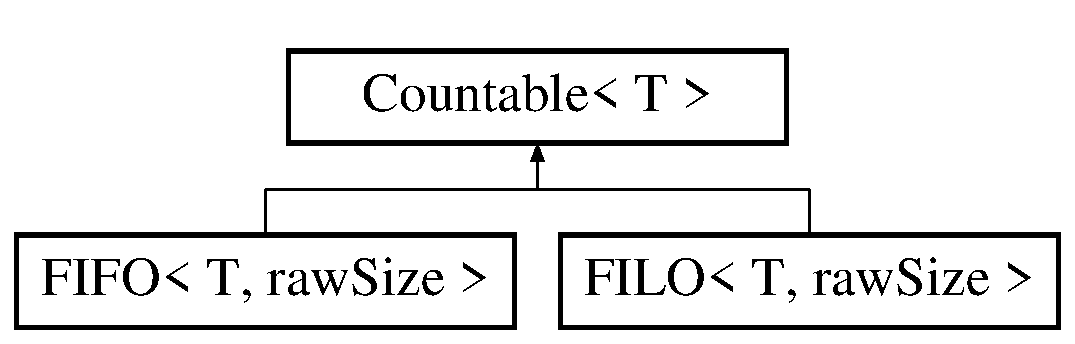
\includegraphics[height=2.000000cm]{class_countable}
\end{center}
\end{figure}
\subsection*{Public Member Functions}
\begin{DoxyCompactItemize}
\item 
\hypertarget{class_countable_a8112c5c4a8de941c8d2dc783fbfe3c7a}{}virtual unsigned int {\bfseries count} () const =0\label{class_countable_a8112c5c4a8de941c8d2dc783fbfe3c7a}

\item 
\hypertarget{class_countable_a86379f5661b5ad88f68c22010c3e6c69}{}virtual const T \& {\bfseries operator\mbox{[}$\,$\mbox{]}} (unsigned int) const =0\label{class_countable_a86379f5661b5ad88f68c22010c3e6c69}

\item 
\hypertarget{class_countable_a9d81652b06fe7bfd6a29e8bde8088d7f}{}virtual T \& {\bfseries operator\mbox{[}$\,$\mbox{]}} (unsigned int)=0\label{class_countable_a9d81652b06fe7bfd6a29e8bde8088d7f}

\item 
\hypertarget{class_countable_a34441ee721d3accbb7169dc04aadaa5f}{}const T \& {\bfseries at} (unsigned int i) const \label{class_countable_a34441ee721d3accbb7169dc04aadaa5f}

\end{DoxyCompactItemize}


The documentation for this class was generated from the following file\+:\begin{DoxyCompactItemize}
\item 
Wiring/Countable.\+h\end{DoxyCompactItemize}

\hypertarget{class_date_time}{}\section{Date\+Time Class Reference}
\label{class_date_time}\index{Date\+Time@{Date\+Time}}
\subsection*{Public Member Functions}
\begin{DoxyCompactItemize}
\item 
\hypertarget{class_date_time_a3c663103e819ac0925be93b06a35931b}{}{\bfseries Date\+Time} (time\+\_\+t time)\label{class_date_time_a3c663103e819ac0925be93b06a35931b}

\item 
\hypertarget{class_date_time_a71771ccc110639ab07f7d91a81a62287}{}{\bfseries operator time\+\_\+t} ()\label{class_date_time_a71771ccc110639ab07f7d91a81a62287}

\item 
\hypertarget{class_date_time_a76cec1408d44dba7b3b9b350e7e93af4}{}void {\bfseries set\+Time} (time\+\_\+t time)\label{class_date_time_a76cec1408d44dba7b3b9b350e7e93af4}

\item 
\hypertarget{class_date_time_a9d7e7be864d50b4049a14956706af5af}{}void {\bfseries set\+Time} (int8\+\_\+t sec, int8\+\_\+t min, int8\+\_\+t hour, int8\+\_\+t day, int8\+\_\+t month, int16\+\_\+t year)\label{class_date_time_a9d7e7be864d50b4049a14956706af5af}

\item 
\hypertarget{class_date_time_aafc5f31a9aab859d6e12553621ed7568}{}bool {\bfseries parse\+Http\+Date} (String http\+Date)\label{class_date_time_aafc5f31a9aab859d6e12553621ed7568}

\item 
\hypertarget{class_date_time_a942983c6d456157328d2efa10e06b9fb}{}bool {\bfseries is\+Null} ()\label{class_date_time_a942983c6d456157328d2efa10e06b9fb}

\item 
\hypertarget{class_date_time_a9e19ab63fe8ee41e00ffee8740a1d29c}{}time\+\_\+t {\bfseries to\+Unix\+Time} ()\label{class_date_time_a9e19ab63fe8ee41e00ffee8740a1d29c}

\item 
\hypertarget{class_date_time_a67ae33e61bac3267c8709e986e5c9865}{}String {\bfseries to\+Short\+Date\+String} ()\label{class_date_time_a67ae33e61bac3267c8709e986e5c9865}

\item 
\hypertarget{class_date_time_ae96f4c5682e7df9a3af768e42d6d3b86}{}String {\bfseries to\+Short\+Time\+String} (bool include\+Seconds=false)\label{class_date_time_ae96f4c5682e7df9a3af768e42d6d3b86}

\item 
\hypertarget{class_date_time_a21f09ede608e518181983b00fa9ed3e9}{}String {\bfseries to\+Full\+Date\+Time\+String} ()\label{class_date_time_a21f09ede608e518181983b00fa9ed3e9}

\item 
\hypertarget{class_date_time_a60d049362b1d16cbe9ceae334ecd56d5}{}void {\bfseries add\+Milliseconds} (long add)\label{class_date_time_a60d049362b1d16cbe9ceae334ecd56d5}

\end{DoxyCompactItemize}
\subsection*{Static Public Member Functions}
\begin{DoxyCompactItemize}
\item 
\hypertarget{class_date_time_a0df39a04d71191364a79249256232539}{}static void {\bfseries convert\+From\+Unix\+Time} (time\+\_\+t timep, int8\+\_\+t $\ast$psec, int8\+\_\+t $\ast$pmin, int8\+\_\+t $\ast$phour, int8\+\_\+t $\ast$pday, int8\+\_\+t $\ast$pwday, int8\+\_\+t $\ast$pmonth, int16\+\_\+t $\ast$pyear)\label{class_date_time_a0df39a04d71191364a79249256232539}

\item 
\hypertarget{class_date_time_acd3d57fa4df25cd12e0f11322a08f8e6}{}static time\+\_\+t {\bfseries convert\+To\+Unix\+Time} (int8\+\_\+t sec, int8\+\_\+t min, int8\+\_\+t hour, int8\+\_\+t day, int8\+\_\+t month, int16\+\_\+t year)\label{class_date_time_acd3d57fa4df25cd12e0f11322a08f8e6}

\end{DoxyCompactItemize}
\subsection*{Public Attributes}
\begin{DoxyCompactItemize}
\item 
\hypertarget{class_date_time_ab306c0dd7931822b39ae58be72cebae0}{}int8\+\_\+t {\bfseries Hour}\label{class_date_time_ab306c0dd7931822b39ae58be72cebae0}

\item 
\hypertarget{class_date_time_a2281ee834b6d9be9fa4c7bc4046394c3}{}int8\+\_\+t {\bfseries Minute}\label{class_date_time_a2281ee834b6d9be9fa4c7bc4046394c3}

\item 
\hypertarget{class_date_time_a05d8e4467eb9841035b31237f3d76a58}{}int8\+\_\+t {\bfseries Second}\label{class_date_time_a05d8e4467eb9841035b31237f3d76a58}

\item 
\hypertarget{class_date_time_a52885b8a894ba0dddabc80bddad467fd}{}int16\+\_\+t {\bfseries Milliseconds}\label{class_date_time_a52885b8a894ba0dddabc80bddad467fd}

\item 
\hypertarget{class_date_time_a8f3d535c712aaa1d8b5cc088ea3c10ff}{}int8\+\_\+t {\bfseries Day}\label{class_date_time_a8f3d535c712aaa1d8b5cc088ea3c10ff}

\item 
\hypertarget{class_date_time_a9a3d78a0f8a1cdbf7df9a026ddea4ee4}{}int8\+\_\+t {\bfseries Dayof\+Week}\label{class_date_time_a9a3d78a0f8a1cdbf7df9a026ddea4ee4}

\item 
\hypertarget{class_date_time_ac2948899151acbee8819a19ad35fd511}{}int8\+\_\+t {\bfseries Month}\label{class_date_time_ac2948899151acbee8819a19ad35fd511}

\item 
\hypertarget{class_date_time_a4d2fdc35a2cc020b1b24ff87d5bf2aeb}{}int16\+\_\+t {\bfseries Year}\label{class_date_time_a4d2fdc35a2cc020b1b24ff87d5bf2aeb}

\end{DoxyCompactItemize}


The documentation for this class was generated from the following files\+:\begin{DoxyCompactItemize}
\item 
Services/\+Date\+Time/Date\+Time.\+h\item 
Services/\+Date\+Time/Date\+Time.\+cpp\end{DoxyCompactItemize}

\hypertarget{class_delegate}{}\section{Delegate$<$ class $>$ Class Template Reference}
\label{class_delegate}\index{Delegate$<$ class $>$@{Delegate$<$ class $>$}}


The documentation for this class was generated from the following file\+:\begin{DoxyCompactItemize}
\item 
Sming\+Core/Delegate.\+h\end{DoxyCompactItemize}

\hypertarget{class_delegate_3_01_return_type_07_params_list_8_8_8_08_4}{}\section{Delegate$<$ Return\+Type(Params\+List...)$>$ Class Template Reference}
\label{class_delegate_3_01_return_type_07_params_list_8_8_8_08_4}\index{Delegate$<$ Return\+Type(\+Params\+List...)$>$@{Delegate$<$ Return\+Type(\+Params\+List...)$>$}}
\subsection*{Public Member Functions}
\begin{DoxyCompactItemize}
\item 
\hypertarget{class_delegate_3_01_return_type_07_params_list_8_8_8_08_4_a6247b01aa81337022d8a1bf14e277200}{}{\footnotesize template$<$class Class\+Type $>$ }\\\+\_\+\+\_\+forceinline {\bfseries Delegate} (Method\+Declaration$<$ Class\+Type $>$ m, Class\+Type $\ast$c)\label{class_delegate_3_01_return_type_07_params_list_8_8_8_08_4_a6247b01aa81337022d8a1bf14e277200}

\item 
\hypertarget{class_delegate_3_01_return_type_07_params_list_8_8_8_08_4_a100786735f37a768328229bfbfd996aa}{}\+\_\+\+\_\+forceinline {\bfseries Delegate} (Function\+Declaration m)\label{class_delegate_3_01_return_type_07_params_list_8_8_8_08_4_a100786735f37a768328229bfbfd996aa}

\item 
\hypertarget{class_delegate_3_01_return_type_07_params_list_8_8_8_08_4_a8351bff2e68b1a1518fa24c28cb66c2d}{}\+\_\+\+\_\+forceinline Return\+Type {\bfseries operator()} (Params\+List...\+params) const \label{class_delegate_3_01_return_type_07_params_list_8_8_8_08_4_a8351bff2e68b1a1518fa24c28cb66c2d}

\item 
\hypertarget{class_delegate_3_01_return_type_07_params_list_8_8_8_08_4_a4edbf1fa0cbac540cf40aa8ef286923c}{}\+\_\+\+\_\+forceinline {\bfseries Delegate} (\hyperlink{class_delegate}{Delegate} \&\&that)\label{class_delegate_3_01_return_type_07_params_list_8_8_8_08_4_a4edbf1fa0cbac540cf40aa8ef286923c}

\item 
\hypertarget{class_delegate_3_01_return_type_07_params_list_8_8_8_08_4_a89d1e09e5e696e9b727436bb84894955}{}\+\_\+\+\_\+forceinline {\bfseries Delegate} (const \hyperlink{class_delegate}{Delegate} \&that)\label{class_delegate_3_01_return_type_07_params_list_8_8_8_08_4_a89d1e09e5e696e9b727436bb84894955}

\item 
\hypertarget{class_delegate_3_01_return_type_07_params_list_8_8_8_08_4_ab8ff021178b0df1abdf02e4757c45530}{}\+\_\+\+\_\+forceinline \hyperlink{class_delegate}{Delegate} \& {\bfseries operator=} (const \hyperlink{class_delegate}{Delegate} \&that)\label{class_delegate_3_01_return_type_07_params_list_8_8_8_08_4_ab8ff021178b0df1abdf02e4757c45530}

\item 
\hypertarget{class_delegate_3_01_return_type_07_params_list_8_8_8_08_4_ac908c5ef8d31cd1589bdb3a94f8b5eff}{}\hyperlink{class_delegate}{Delegate} \& {\bfseries operator=} (\hyperlink{class_delegate}{Delegate} \&\&that)\label{class_delegate_3_01_return_type_07_params_list_8_8_8_08_4_ac908c5ef8d31cd1589bdb3a94f8b5eff}

\item 
\hypertarget{class_delegate_3_01_return_type_07_params_list_8_8_8_08_4_af757bbda83d6ff9bf7e4b869888cb962}{}\+\_\+\+\_\+forceinline {\bfseries operator bool} () const \label{class_delegate_3_01_return_type_07_params_list_8_8_8_08_4_af757bbda83d6ff9bf7e4b869888cb962}

\end{DoxyCompactItemize}
\subsection*{Protected Member Functions}
\begin{DoxyCompactItemize}
\item 
\hypertarget{class_delegate_3_01_return_type_07_params_list_8_8_8_08_4_ac9ef56d176dd819c6080055f911f5275}{}void {\bfseries copy} (const \hyperlink{class_delegate}{Delegate} \&other)\label{class_delegate_3_01_return_type_07_params_list_8_8_8_08_4_ac9ef56d176dd819c6080055f911f5275}

\end{DoxyCompactItemize}


The documentation for this class was generated from the following file\+:\begin{DoxyCompactItemize}
\item 
Sming\+Core/Delegate.\+h\end{DoxyCompactItemize}

\hypertarget{structdhcps__lease}{}\section{dhcps\+\_\+lease Struct Reference}
\label{structdhcps__lease}\index{dhcps\+\_\+lease@{dhcps\+\_\+lease}}
\subsection*{Public Attributes}
\begin{DoxyCompactItemize}
\item 
\hypertarget{structdhcps__lease_a0b4d301e6eb86332afa43e0488492026}{}uint32 {\bfseries start\+\_\+ip}\label{structdhcps__lease_a0b4d301e6eb86332afa43e0488492026}

\item 
\hypertarget{structdhcps__lease_a9f82e2fe01b1e1e0abe25c513bfc2d10}{}uint32 {\bfseries end\+\_\+ip}\label{structdhcps__lease_a9f82e2fe01b1e1e0abe25c513bfc2d10}

\end{DoxyCompactItemize}


The documentation for this struct was generated from the following file\+:\begin{DoxyCompactItemize}
\item 
system/include/lwip/app/dhcpserver.\+h\end{DoxyCompactItemize}

\hypertarget{structdhcps__msg}{}\section{dhcps\+\_\+msg Struct Reference}
\label{structdhcps__msg}\index{dhcps\+\_\+msg@{dhcps\+\_\+msg}}
\subsection*{Public Attributes}
\begin{DoxyCompactItemize}
\item 
\hypertarget{structdhcps__msg_a09df11b5e009ebc7ecf7b97d07de6cb2}{}uint8\+\_\+t {\bfseries op}\label{structdhcps__msg_a09df11b5e009ebc7ecf7b97d07de6cb2}

\item 
\hypertarget{structdhcps__msg_a7a2065a67b9490d40ba2150582e5b7fe}{}uint8\+\_\+t {\bfseries htype}\label{structdhcps__msg_a7a2065a67b9490d40ba2150582e5b7fe}

\item 
\hypertarget{structdhcps__msg_a66ad803d7d8b515703eb1eccc78e1169}{}uint8\+\_\+t {\bfseries hlen}\label{structdhcps__msg_a66ad803d7d8b515703eb1eccc78e1169}

\item 
\hypertarget{structdhcps__msg_a38e1eaffaf9c0704575326c682463962}{}uint8\+\_\+t {\bfseries hops}\label{structdhcps__msg_a38e1eaffaf9c0704575326c682463962}

\item 
\hypertarget{structdhcps__msg_ad7467887b13b869f299e29df8cb6ec83}{}uint8\+\_\+t {\bfseries xid} \mbox{[}4\mbox{]}\label{structdhcps__msg_ad7467887b13b869f299e29df8cb6ec83}

\item 
\hypertarget{structdhcps__msg_a90b2c88d35a395c8d64753387f8ef467}{}uint16\+\_\+t {\bfseries secs}\label{structdhcps__msg_a90b2c88d35a395c8d64753387f8ef467}

\item 
\hypertarget{structdhcps__msg_a66dd2318b7f49f2f6010c0e649c50060}{}uint16\+\_\+t {\bfseries flags}\label{structdhcps__msg_a66dd2318b7f49f2f6010c0e649c50060}

\item 
\hypertarget{structdhcps__msg_acdac0ca224de1b070dcff6ca700827b5}{}uint8\+\_\+t {\bfseries ciaddr} \mbox{[}4\mbox{]}\label{structdhcps__msg_acdac0ca224de1b070dcff6ca700827b5}

\item 
\hypertarget{structdhcps__msg_a906900ceeb4a41eea74d01da620fb0d6}{}uint8\+\_\+t {\bfseries yiaddr} \mbox{[}4\mbox{]}\label{structdhcps__msg_a906900ceeb4a41eea74d01da620fb0d6}

\item 
\hypertarget{structdhcps__msg_af7beef08ac8c5e7e0fad0be480d03663}{}uint8\+\_\+t {\bfseries siaddr} \mbox{[}4\mbox{]}\label{structdhcps__msg_af7beef08ac8c5e7e0fad0be480d03663}

\item 
\hypertarget{structdhcps__msg_ab151af5816632c4e4784224c7d92f8b8}{}uint8\+\_\+t {\bfseries giaddr} \mbox{[}4\mbox{]}\label{structdhcps__msg_ab151af5816632c4e4784224c7d92f8b8}

\item 
\hypertarget{structdhcps__msg_aa972ae11efcd0dd4b26df3b9998626ca}{}uint8\+\_\+t {\bfseries chaddr} \mbox{[}16\mbox{]}\label{structdhcps__msg_aa972ae11efcd0dd4b26df3b9998626ca}

\item 
\hypertarget{structdhcps__msg_a37c6d315b6994f09c83d322d88a3585a}{}uint8\+\_\+t {\bfseries sname} \mbox{[}64\mbox{]}\label{structdhcps__msg_a37c6d315b6994f09c83d322d88a3585a}

\item 
\hypertarget{structdhcps__msg_a7006a9f5d8833d1baccd1075b6633cce}{}uint8\+\_\+t {\bfseries file} \mbox{[}128\mbox{]}\label{structdhcps__msg_a7006a9f5d8833d1baccd1075b6633cce}

\item 
\hypertarget{structdhcps__msg_abe3aae356c401b4ff83d402309564ae4}{}uint8\+\_\+t {\bfseries options} \mbox{[}312\mbox{]}\label{structdhcps__msg_abe3aae356c401b4ff83d402309564ae4}

\end{DoxyCompactItemize}


The documentation for this struct was generated from the following file\+:\begin{DoxyCompactItemize}
\item 
system/include/lwip/app/dhcpserver.\+h\end{DoxyCompactItemize}

\hypertarget{structdhcps__pool}{}\section{dhcps\+\_\+pool Struct Reference}
\label{structdhcps__pool}\index{dhcps\+\_\+pool@{dhcps\+\_\+pool}}
\subsection*{Public Attributes}
\begin{DoxyCompactItemize}
\item 
\hypertarget{structdhcps__pool_af5df9203d2aa88d46c999e72c58328a1}{}struct \hyperlink{structip__addr}{ip\+\_\+addr} {\bfseries ip}\label{structdhcps__pool_af5df9203d2aa88d46c999e72c58328a1}

\item 
\hypertarget{structdhcps__pool_a637720fc6135600eb84c14ff7f0bb864}{}uint8 {\bfseries mac} \mbox{[}6\mbox{]}\label{structdhcps__pool_a637720fc6135600eb84c14ff7f0bb864}

\item 
\hypertarget{structdhcps__pool_a2c76ad0519e095a759b497b3bd88c34f}{}uint32 {\bfseries lease\+\_\+timer}\label{structdhcps__pool_a2c76ad0519e095a759b497b3bd88c34f}

\end{DoxyCompactItemize}


The documentation for this struct was generated from the following file\+:\begin{DoxyCompactItemize}
\item 
system/include/lwip/app/dhcpserver.\+h\end{DoxyCompactItemize}

\hypertarget{structdhcps__state}{}\section{dhcps\+\_\+state Struct Reference}
\label{structdhcps__state}\index{dhcps\+\_\+state@{dhcps\+\_\+state}}
\subsection*{Public Attributes}
\begin{DoxyCompactItemize}
\item 
\hypertarget{structdhcps__state_a37f65b6dae98b17868e3d2737bc1b35b}{}sint16\+\_\+t {\bfseries state}\label{structdhcps__state_a37f65b6dae98b17868e3d2737bc1b35b}

\end{DoxyCompactItemize}


The documentation for this struct was generated from the following file\+:\begin{DoxyCompactItemize}
\item 
system/include/lwip/app/dhcpserver.\+h\end{DoxyCompactItemize}

\hypertarget{class_d_h_t}{}\section{D\+H\+T Class Reference}
\label{class_d_h_t}\index{D\+H\+T@{D\+H\+T}}
\subsection*{Public Member Functions}
\begin{DoxyCompactItemize}
\item 
\hypertarget{class_d_h_t_ab1c7a78d57ca914a0603c10518d834e6}{}{\bfseries D\+H\+T} (uint8\+\_\+t pin, uint8\+\_\+t type, uint8\+\_\+t count=C\+O\+U\+N\+T\+\_\+\+R\+E\+C\+A\+L\+C\+U\+L\+A\+T\+E\+D\+\_\+\+F\+O\+R\+\_\+\+D\+E\+F\+A\+U\+L\+T\+\_\+\+E\+S\+P\+\_\+\+F\+R\+E\+Q\+U\+E\+N\+C\+Y)\label{class_d_h_t_ab1c7a78d57ca914a0603c10518d834e6}

\item 
\hypertarget{class_d_h_t_a757dc4b34611c08168248b276e4f84a8}{}void {\bfseries begin} (void)\label{class_d_h_t_a757dc4b34611c08168248b276e4f84a8}

\item 
\hypertarget{class_d_h_t_a221e8b5b7b2147be0cdd16f2b6344a26}{}float {\bfseries read\+Temperature} (bool S=false)\label{class_d_h_t_a221e8b5b7b2147be0cdd16f2b6344a26}

\item 
\hypertarget{class_d_h_t_a582df4d39cd56b4acbd47fbe75aedcc3}{}float {\bfseries convert\+Cto\+F} (float)\label{class_d_h_t_a582df4d39cd56b4acbd47fbe75aedcc3}

\item 
\hypertarget{class_d_h_t_a23bfb1643c202289efcf8f5a86717a9c}{}float {\bfseries read\+Humidity} (void)\label{class_d_h_t_a23bfb1643c202289efcf8f5a86717a9c}

\end{DoxyCompactItemize}


The documentation for this class was generated from the following files\+:\begin{DoxyCompactItemize}
\item 
Libraries/\+D\+H\+T/D\+H\+T.\+h\item 
Libraries/\+D\+H\+T/D\+H\+T.\+cpp\end{DoxyCompactItemize}

\hypertarget{class_display}{}\section{Display Class Reference}
\label{class_display}\index{Display@{Display}}
Inheritance diagram for Display\+:\begin{figure}[H]
\begin{center}
\leavevmode
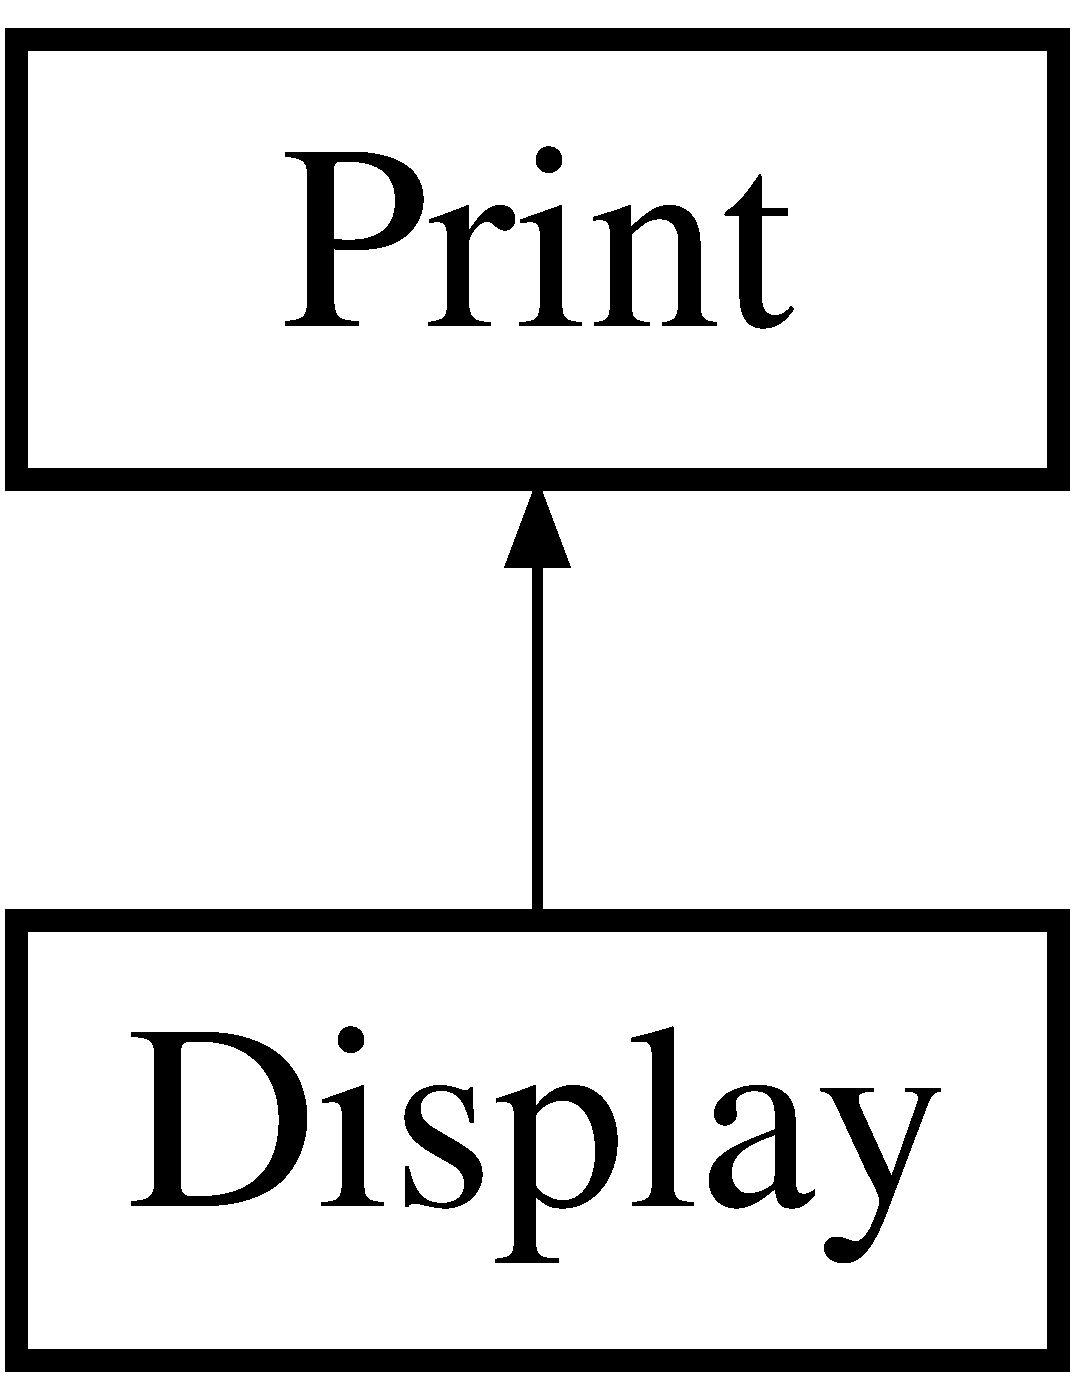
\includegraphics[height=2.000000cm]{class_display}
\end{center}
\end{figure}
\subsection*{Public Member Functions}
\begin{DoxyCompactItemize}
\item 
\hypertarget{class_display_a0e3959fe9671746b0331e75f8d9f23e6}{}virtual void {\bfseries clear} (void)=0\label{class_display_a0e3959fe9671746b0331e75f8d9f23e6}

\item 
\hypertarget{class_display_a45f233e66569e797e6ad87c0338da56b}{}virtual void {\bfseries home} (void)=0\label{class_display_a45f233e66569e797e6ad87c0338da56b}

\item 
\hypertarget{class_display_ae782c76bdbef3b36574c327ebd1340b4}{}virtual void {\bfseries set\+Cursor} (uint8\+\_\+t, uint8\+\_\+t)=0\label{class_display_ae782c76bdbef3b36574c327ebd1340b4}

\end{DoxyCompactItemize}


The documentation for this class was generated from the following file\+:\begin{DoxyCompactItemize}
\item 
Wiring/Display.\+h\end{DoxyCompactItemize}

\hypertarget{struct_dns_lookup}{}\section{Dns\+Lookup Struct Reference}
\label{struct_dns_lookup}\index{Dns\+Lookup@{Dns\+Lookup}}
\subsection*{Public Attributes}
\begin{DoxyCompactItemize}
\item 
\hypertarget{struct_dns_lookup_a2dec6ffc62c9f47e2bbbca31eaed2331}{}\hyperlink{class_tcp_connection}{Tcp\+Connection} $\ast$ {\bfseries con}\label{struct_dns_lookup_a2dec6ffc62c9f47e2bbbca31eaed2331}

\item 
\hypertarget{struct_dns_lookup_a6d7ab4b2930160344759a00c0f37d3b3}{}int {\bfseries port}\label{struct_dns_lookup_a6d7ab4b2930160344759a00c0f37d3b3}

\end{DoxyCompactItemize}


The documentation for this struct was generated from the following file\+:\begin{DoxyCompactItemize}
\item 
Sming\+Core/\+Network/Net\+Utils.\+h\end{DoxyCompactItemize}

\hypertarget{class_driver_p_w_m}{}\section{Driver\+P\+W\+M Class Reference}
\label{class_driver_p_w_m}\index{Driver\+P\+W\+M@{Driver\+P\+W\+M}}


If you want to use P\+W\+M -\/ this class if for you.  




{\ttfamily \#include $<$P\+W\+M.\+h$>$}

\subsection*{Public Member Functions}
\begin{DoxyCompactItemize}
\item 
\hypertarget{class_driver_p_w_m_acffe6831e34675b688eca8b016c815cd}{}\hyperlink{class_driver_p_w_m_acffe6831e34675b688eca8b016c815cd}{Driver\+P\+W\+M} ()\label{class_driver_p_w_m_acffe6831e34675b688eca8b016c815cd}

\begin{DoxyCompactList}\small\item\em generates instance of class -\/ nothing cool \end{DoxyCompactList}\item 
\hypertarget{class_driver_p_w_m_a4c2173c8d360f3581ebc81f6a3a0bdb1}{}void \hyperlink{class_driver_p_w_m_a4c2173c8d360f3581ebc81f6a3a0bdb1}{initialize} ()\label{class_driver_p_w_m_a4c2173c8d360f3581ebc81f6a3a0bdb1}

\begin{DoxyCompactList}\small\item\em Initializes P\+W\+M -\/ no need to call it before using pwm. \end{DoxyCompactList}\item 
\hypertarget{class_driver_p_w_m_abf80bffdbf8f2fe60bd58d132457cf73}{}void \hyperlink{class_driver_p_w_m_abf80bffdbf8f2fe60bd58d132457cf73}{analog\+Write} (uint8\+\_\+t pin, int duty)\label{class_driver_p_w_m_abf80bffdbf8f2fe60bd58d132457cf73}

\begin{DoxyCompactList}\small\item\em starts P\+W\+M on pin \end{DoxyCompactList}\item 
\hypertarget{class_driver_p_w_m_a202cd541c9f1b791129e63f01c9a1c2b}{}void \hyperlink{class_driver_p_w_m_a202cd541c9f1b791129e63f01c9a1c2b}{no\+Analog\+Write} (uint8\+\_\+t pin)\label{class_driver_p_w_m_a202cd541c9f1b791129e63f01c9a1c2b}

\begin{DoxyCompactList}\small\item\em stops P\+W\+M on pin \end{DoxyCompactList}\end{DoxyCompactItemize}
\subsection*{Static Protected Member Functions}
\begin{DoxyCompactItemize}
\item 
\hypertarget{class_driver_p_w_m_a9e162932cc04fbbb7d3e6a093b9daa1d}{}static void I\+R\+A\+M\+\_\+\+A\+T\+T\+R {\bfseries processing\+Static} (void $\ast$arg)\label{class_driver_p_w_m_a9e162932cc04fbbb7d3e6a093b9daa1d}

\end{DoxyCompactItemize}


\subsection{Detailed Description}
If you want to use P\+W\+M -\/ this class if for you. 

To use it just use it! 

The documentation for this class was generated from the following files\+:\begin{DoxyCompactItemize}
\item 
Sming\+Core/P\+W\+M.\+h\item 
Sming\+Core/P\+W\+M.\+cpp\end{DoxyCompactItemize}

\hypertarget{class_arduino_json_1_1_dynamic_json_buffer}{}\section{Arduino\+Json\+:\+:Dynamic\+Json\+Buffer Class Reference}
\label{class_arduino_json_1_1_dynamic_json_buffer}\index{Arduino\+Json\+::\+Dynamic\+Json\+Buffer@{Arduino\+Json\+::\+Dynamic\+Json\+Buffer}}
Inheritance diagram for Arduino\+Json\+:\+:Dynamic\+Json\+Buffer\+:\begin{figure}[H]
\begin{center}
\leavevmode
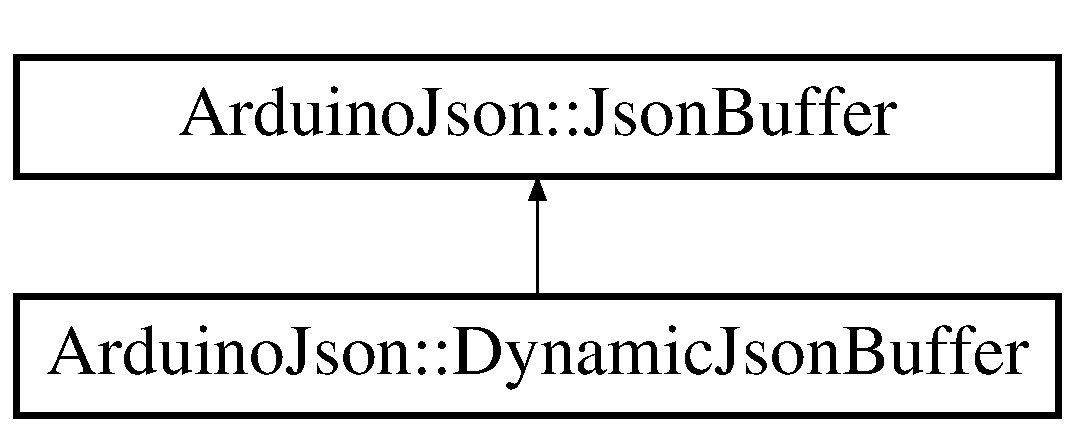
\includegraphics[height=2.000000cm]{class_arduino_json_1_1_dynamic_json_buffer}
\end{center}
\end{figure}
\subsection*{Public Member Functions}
\begin{DoxyCompactItemize}
\item 
\hypertarget{class_arduino_json_1_1_dynamic_json_buffer_a584f47a4b7272d8bc95b055e49130128}{}size\+\_\+t {\bfseries size} () const \label{class_arduino_json_1_1_dynamic_json_buffer_a584f47a4b7272d8bc95b055e49130128}

\item 
\hypertarget{class_arduino_json_1_1_dynamic_json_buffer_ad211820641812756fc310267d24ae587}{}size\+\_\+t {\bfseries block\+Count} () const \label{class_arduino_json_1_1_dynamic_json_buffer_ad211820641812756fc310267d24ae587}

\end{DoxyCompactItemize}
\subsection*{Static Public Attributes}
\begin{DoxyCompactItemize}
\item 
\hypertarget{class_arduino_json_1_1_dynamic_json_buffer_a88eb6738f9e6f66d1b1d5907220c3583}{}static const size\+\_\+t {\bfseries B\+L\+O\+C\+K\+\_\+\+C\+A\+P\+A\+C\+I\+T\+Y} = 128\label{class_arduino_json_1_1_dynamic_json_buffer_a88eb6738f9e6f66d1b1d5907220c3583}

\end{DoxyCompactItemize}
\subsection*{Protected Member Functions}
\begin{DoxyCompactItemize}
\item 
\hypertarget{class_arduino_json_1_1_dynamic_json_buffer_a961d001c640fe6481b6f90798b115bdb}{}virtual void $\ast$ {\bfseries alloc} (size\+\_\+t bytes)\label{class_arduino_json_1_1_dynamic_json_buffer_a961d001c640fe6481b6f90798b115bdb}

\end{DoxyCompactItemize}


The documentation for this class was generated from the following file\+:\begin{DoxyCompactItemize}
\item 
Services/\+Arduino\+Json/include/\+Arduino\+Json/Dynamic\+Json\+Buffer.\+hpp\end{DoxyCompactItemize}

\hypertarget{class_e_s_p01___description}{}\section{E\+S\+P01\+\_\+\+Description Class Reference}
\label{class_e_s_p01___description}\index{E\+S\+P01\+\_\+\+Description@{E\+S\+P01\+\_\+\+Description}}
\subsection*{Public Attributes}
\begin{DoxyCompactItemize}
\item 
\hypertarget{class_e_s_p01___description_a2a827569281a4568f101e31d4f2721ea}{}\hyperlink{struct_esp_digital_pin}{Esp\+Digital\+Pin} {\bfseries gpio0} = Esp\+Digital\+Pins\mbox{[}0\mbox{]}\label{class_e_s_p01___description_a2a827569281a4568f101e31d4f2721ea}

\item 
\hypertarget{class_e_s_p01___description_a8ab8a331db4d6c03147049d9aaa62759}{}\hyperlink{struct_esp_digital_pin}{Esp\+Digital\+Pin} {\bfseries gpio2} = Esp\+Digital\+Pins\mbox{[}2\mbox{]}\label{class_e_s_p01___description_a8ab8a331db4d6c03147049d9aaa62759}

\item 
\hypertarget{class_e_s_p01___description_a563919a8fe237a6ad231f9733b3a264a}{}\hyperlink{struct_esp_digital_pin}{Esp\+Digital\+Pin} {\bfseries tx} = Esp\+Digital\+Pins\mbox{[}1\mbox{]}\label{class_e_s_p01___description_a563919a8fe237a6ad231f9733b3a264a}

\item 
\hypertarget{class_e_s_p01___description_a8baf1743bfc916f889f0e8dca52d2abe}{}\hyperlink{struct_esp_digital_pin}{Esp\+Digital\+Pin} {\bfseries rx} = Esp\+Digital\+Pins\mbox{[}3\mbox{]}\label{class_e_s_p01___description_a8baf1743bfc916f889f0e8dca52d2abe}

\end{DoxyCompactItemize}


The documentation for this class was generated from the following file\+:\begin{DoxyCompactItemize}
\item 
Sming\+Core/Boards.\+h\end{DoxyCompactItemize}

\hypertarget{structespconn}{}\section{espconn Struct Reference}
\label{structespconn}\index{espconn@{espconn}}


{\ttfamily \#include $<$espconn.\+h$>$}

\subsection*{Public Attributes}
\begin{DoxyCompactItemize}
\item 
enum espconn\+\_\+type \hyperlink{structespconn_a393c997ab67360b4e17485123518595c}{type}
\item 
enum espconn\+\_\+state \hyperlink{structespconn_a613ca239a3e312e72b5a593076af30b7}{state}
\item 
\hypertarget{structespconn_afb66ba2a45e0c2c7aa089619d909a335}{}\begin{tabbing}
xx\=xx\=xx\=xx\=xx\=xx\=xx\=xx\=xx\=\kill
union \{\\
\>\hyperlink{struct__esp__tcp}{esp\_tcp} $\ast$ {\bfseries tcp}\\
\>\hyperlink{struct__esp__udp}{esp\_udp} $\ast$ {\bfseries udp}\\
\} {\bfseries proto}\label{structespconn_afb66ba2a45e0c2c7aa089619d909a335}
\\

\end{tabbing}\item 
espconn\+\_\+recv\+\_\+callback \hyperlink{structespconn_a89f6cc886a70f9b844093673f2083f00}{recv\+\_\+callback}
\item 
\hypertarget{structespconn_a945c23f67172f92d557a11ecf78da108}{}espconn\+\_\+sent\+\_\+callback {\bfseries sent\+\_\+callback}\label{structespconn_a945c23f67172f92d557a11ecf78da108}

\item 
\hypertarget{structespconn_a8df3d7d2a7153aa96ce6b022da5050ab}{}uint8 {\bfseries link\+\_\+cnt}\label{structespconn_a8df3d7d2a7153aa96ce6b022da5050ab}

\item 
\hypertarget{structespconn_a7298e6238b12e95329157f5c82f0187e}{}void $\ast$ {\bfseries reverse}\label{structespconn_a7298e6238b12e95329157f5c82f0187e}

\end{DoxyCompactItemize}


\subsection{Detailed Description}
A espconn descriptor 

\subsection{Member Data Documentation}
\hypertarget{structespconn_a89f6cc886a70f9b844093673f2083f00}{}\index{espconn@{espconn}!recv\+\_\+callback@{recv\+\_\+callback}}
\index{recv\+\_\+callback@{recv\+\_\+callback}!espconn@{espconn}}
\subsubsection[{recv\+\_\+callback}]{\setlength{\rightskip}{0pt plus 5cm}espconn\+\_\+recv\+\_\+callback espconn\+::recv\+\_\+callback}\label{structespconn_a89f6cc886a70f9b844093673f2083f00}
A callback function that is informed about events for this espconn \hypertarget{structespconn_a613ca239a3e312e72b5a593076af30b7}{}\index{espconn@{espconn}!state@{state}}
\index{state@{state}!espconn@{espconn}}
\subsubsection[{state}]{\setlength{\rightskip}{0pt plus 5cm}enum espconn\+\_\+state espconn\+::state}\label{structespconn_a613ca239a3e312e72b5a593076af30b7}
current state of the espconn \hypertarget{structespconn_a393c997ab67360b4e17485123518595c}{}\index{espconn@{espconn}!type@{type}}
\index{type@{type}!espconn@{espconn}}
\subsubsection[{type}]{\setlength{\rightskip}{0pt plus 5cm}enum espconn\+\_\+type espconn\+::type}\label{structespconn_a393c997ab67360b4e17485123518595c}
type of the espconn (T\+C\+P, U\+D\+P) 

The documentation for this struct was generated from the following file\+:\begin{DoxyCompactItemize}
\item 
system/include/lwip/app/espconn.\+h\end{DoxyCompactItemize}

\hypertarget{struct_esp_digital_pin}{}\section{Esp\+Digital\+Pin Struct Reference}
\label{struct_esp_digital_pin}\index{Esp\+Digital\+Pin@{Esp\+Digital\+Pin}}
\subsection*{Public Member Functions}
\begin{DoxyCompactItemize}
\item 
\hypertarget{struct_esp_digital_pin_a71781517b5a9fda73c20d4b12e7ef001}{}{\bfseries operator const int} ()\label{struct_esp_digital_pin_a71781517b5a9fda73c20d4b12e7ef001}

\item 
\hypertarget{struct_esp_digital_pin_abac51068cde6205783b1cc9ab25ff5dc}{}void {\bfseries mode} (uint8\+\_\+t mode)\label{struct_esp_digital_pin_abac51068cde6205783b1cc9ab25ff5dc}

\item 
\hypertarget{struct_esp_digital_pin_a34c567b8e1d4a786e9721f92fa46e8f0}{}void {\bfseries write} (uint8\+\_\+t val)\label{struct_esp_digital_pin_a34c567b8e1d4a786e9721f92fa46e8f0}

\item 
\hypertarget{struct_esp_digital_pin_a46915f0b619f6692a98bac1255f6bbba}{}uint8\+\_\+t {\bfseries read} ()\label{struct_esp_digital_pin_a46915f0b619f6692a98bac1255f6bbba}

\end{DoxyCompactItemize}
\subsection*{Public Attributes}
\begin{DoxyCompactItemize}
\item 
\hypertarget{struct_esp_digital_pin_a3b394ffa61ba1a684eff0f3e2c505aea}{}uint8\+\_\+t {\bfseries id}\label{struct_esp_digital_pin_a3b394ffa61ba1a684eff0f3e2c505aea}

\item 
\hypertarget{struct_esp_digital_pin_ace65e413174da7e2941dc24035d02bae}{}uint32\+\_\+t {\bfseries mux}\label{struct_esp_digital_pin_ace65e413174da7e2941dc24035d02bae}

\item 
\hypertarget{struct_esp_digital_pin_a109e7d4c694bfc34924cbb0f4fe3123c}{}uint8\+\_\+t {\bfseries gpio\+Func}\label{struct_esp_digital_pin_a109e7d4c694bfc34924cbb0f4fe3123c}

\end{DoxyCompactItemize}


The documentation for this struct was generated from the following files\+:\begin{DoxyCompactItemize}
\item 
Sming\+Core/E\+S\+P8266\+E\+X.\+h\item 
Sming\+Core/E\+S\+P8266\+E\+X.\+cpp\end{DoxyCompactItemize}

\hypertarget{class_f_i_f_o}{}\section{F\+I\+F\+O$<$ T, raw\+Size $>$ Class Template Reference}
\label{class_f_i_f_o}\index{F\+I\+F\+O$<$ T, raw\+Size $>$@{F\+I\+F\+O$<$ T, raw\+Size $>$}}
Inheritance diagram for F\+I\+F\+O$<$ T, raw\+Size $>$\+:\begin{figure}[H]
\begin{center}
\leavevmode
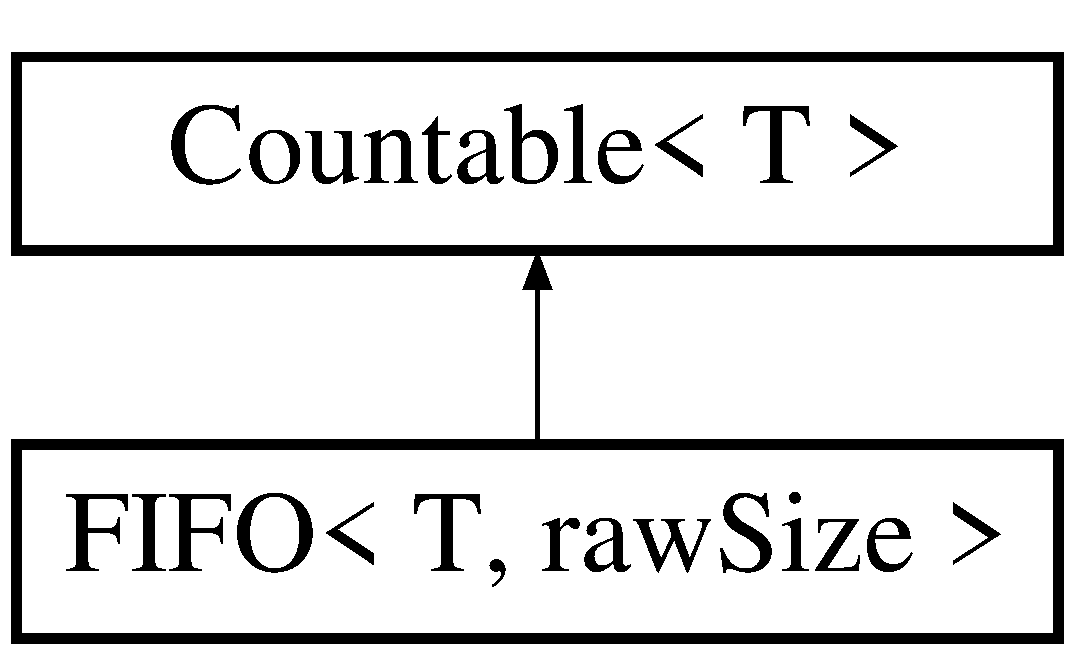
\includegraphics[height=2.000000cm]{class_f_i_f_o}
\end{center}
\end{figure}
\subsection*{Public Member Functions}
\begin{DoxyCompactItemize}
\item 
\hypertarget{class_f_i_f_o_a8cbc6e8fe109581b7dad5bc0b69f5326}{}T {\bfseries dequeue} ()\label{class_f_i_f_o_a8cbc6e8fe109581b7dad5bc0b69f5326}

\item 
\hypertarget{class_f_i_f_o_aae0f318e05930819896ad50075a2e3b7}{}bool {\bfseries enqueue} (T element)\label{class_f_i_f_o_aae0f318e05930819896ad50075a2e3b7}

\item 
\hypertarget{class_f_i_f_o_aea09087d6916d1da1ad26c572deeb250}{}T {\bfseries peek} () const \label{class_f_i_f_o_aea09087d6916d1da1ad26c572deeb250}

\item 
\hypertarget{class_f_i_f_o_ae6bf4ed61af9e534f29ed450f5207702}{}void {\bfseries flush} ()\label{class_f_i_f_o_ae6bf4ed61af9e534f29ed450f5207702}

\item 
\hypertarget{class_f_i_f_o_a822ba9631279ff47cd843a5273a101f8}{}unsigned int {\bfseries count} () const \label{class_f_i_f_o_a822ba9631279ff47cd843a5273a101f8}

\item 
\hypertarget{class_f_i_f_o_af640bb36ab136ea226538e333e97c878}{}const T \& {\bfseries operator\mbox{[}$\,$\mbox{]}} (unsigned int index) const \label{class_f_i_f_o_af640bb36ab136ea226538e333e97c878}

\item 
\hypertarget{class_f_i_f_o_a8704685595a6d464c66ccce3a3b94a6b}{}T \& {\bfseries operator\mbox{[}$\,$\mbox{]}} (unsigned int index)\label{class_f_i_f_o_a8704685595a6d464c66ccce3a3b94a6b}

\end{DoxyCompactItemize}
\subsection*{Public Attributes}
\begin{DoxyCompactItemize}
\item 
\hypertarget{class_f_i_f_o_a538df52632ac71e5007802fe5a7435ae}{}const int {\bfseries size}\label{class_f_i_f_o_a538df52632ac71e5007802fe5a7435ae}

\end{DoxyCompactItemize}


The documentation for this class was generated from the following file\+:\begin{DoxyCompactItemize}
\item 
Wiring/F\+I\+F\+O.\+h\end{DoxyCompactItemize}

\hypertarget{class_file_stream}{}\section{File\+Stream Class Reference}
\label{class_file_stream}\index{File\+Stream@{File\+Stream}}
Inheritance diagram for File\+Stream\+:\begin{figure}[H]
\begin{center}
\leavevmode
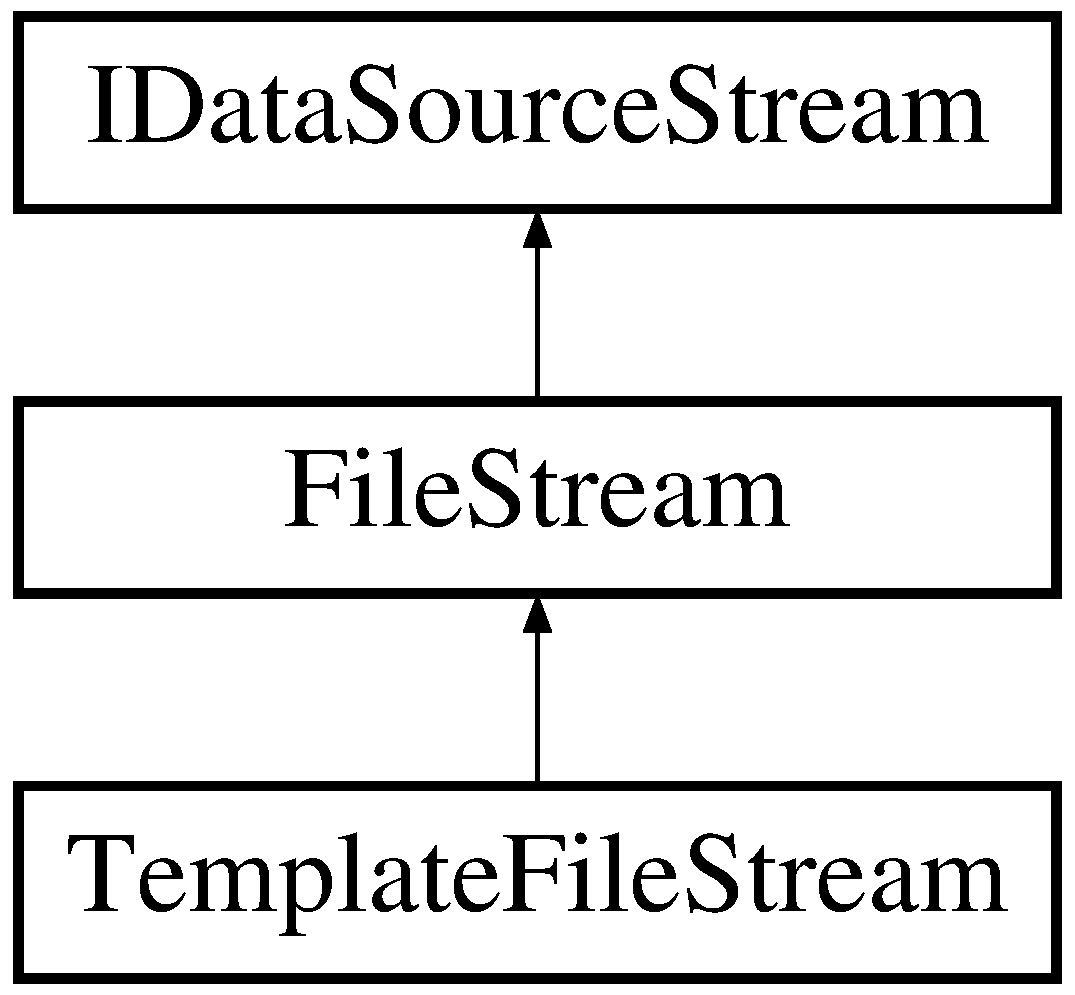
\includegraphics[height=3.000000cm]{class_file_stream}
\end{center}
\end{figure}
\subsection*{Public Member Functions}
\begin{DoxyCompactItemize}
\item 
\hypertarget{class_file_stream_a4cd4eca5016e95f3ffb41a29b3214d41}{}{\bfseries File\+Stream} (String file\+Name)\label{class_file_stream_a4cd4eca5016e95f3ffb41a29b3214d41}

\item 
\hypertarget{class_file_stream_adfb9c8efcb62d6f2cc91ca4efbad718d}{}virtual Stream\+Type {\bfseries get\+Stream\+Type} ()\label{class_file_stream_adfb9c8efcb62d6f2cc91ca4efbad718d}

\item 
\hypertarget{class_file_stream_a49eff9c8d564f58a836c646a9c9ebe05}{}virtual uint16\+\_\+t {\bfseries get\+Data\+Pointer} (char $\ast$$\ast$data)\label{class_file_stream_a49eff9c8d564f58a836c646a9c9ebe05}

\item 
\hypertarget{class_file_stream_aef7c57fb24daebcddf60f62581e2b10b}{}virtual bool {\bfseries seek} (int len)\label{class_file_stream_aef7c57fb24daebcddf60f62581e2b10b}

\item 
\hypertarget{class_file_stream_ad090f9e130a0b3a9888844a61ab02f38}{}virtual bool {\bfseries is\+Finished} ()\label{class_file_stream_ad090f9e130a0b3a9888844a61ab02f38}

\item 
\hypertarget{class_file_stream_acf13ae992e4b99b244633dc8d592311b}{}String {\bfseries file\+Name} ()\label{class_file_stream_acf13ae992e4b99b244633dc8d592311b}

\item 
\hypertarget{class_file_stream_a34cab4c00d5b49e16aeffc84c34970f5}{}bool {\bfseries file\+Exist} ()\label{class_file_stream_a34cab4c00d5b49e16aeffc84c34970f5}

\item 
\hypertarget{class_file_stream_aca0218676383112bf4c034d98461f682}{}int {\bfseries get\+Pos} ()\label{class_file_stream_aca0218676383112bf4c034d98461f682}

\end{DoxyCompactItemize}


The documentation for this class was generated from the following files\+:\begin{DoxyCompactItemize}
\item 
Sming\+Core/Data\+Source\+Stream.\+h\item 
Sming\+Core/Data\+Source\+Stream.\+cpp\end{DoxyCompactItemize}

\hypertarget{class_f_i_l_o}{}\section{F\+I\+L\+O$<$ T, raw\+Size $>$ Class Template Reference}
\label{class_f_i_l_o}\index{F\+I\+L\+O$<$ T, raw\+Size $>$@{F\+I\+L\+O$<$ T, raw\+Size $>$}}
Inheritance diagram for F\+I\+L\+O$<$ T, raw\+Size $>$\+:\begin{figure}[H]
\begin{center}
\leavevmode
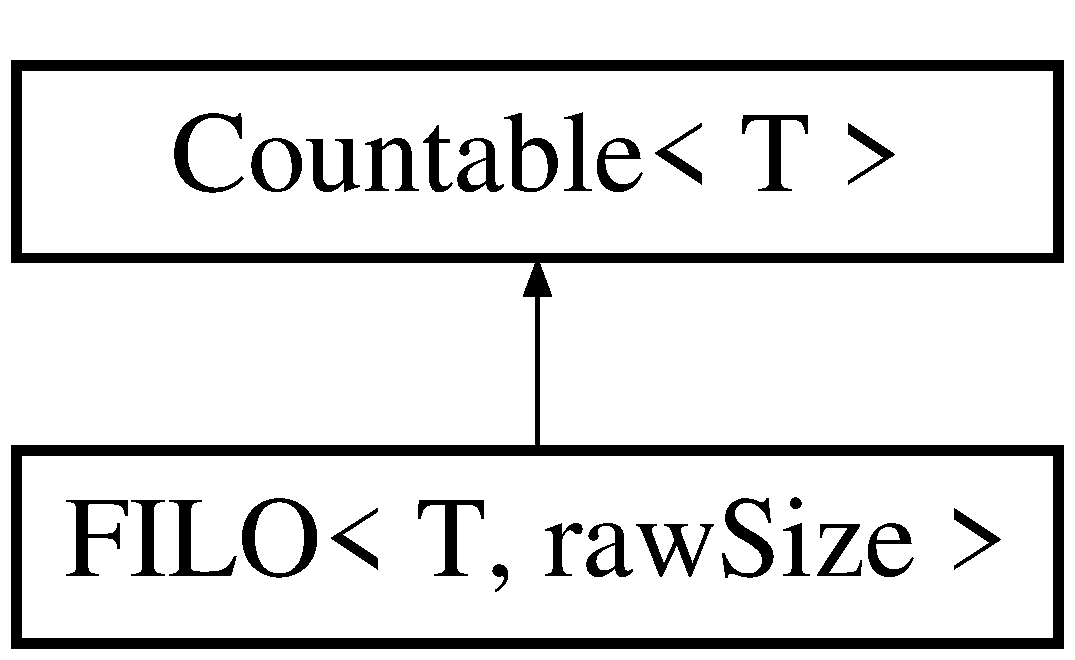
\includegraphics[height=2.000000cm]{class_f_i_l_o}
\end{center}
\end{figure}
\subsection*{Public Member Functions}
\begin{DoxyCompactItemize}
\item 
\hypertarget{class_f_i_l_o_ac71e64def1cb48cbe79d7d86b227957f}{}T {\bfseries pop} ()\label{class_f_i_l_o_ac71e64def1cb48cbe79d7d86b227957f}

\item 
\hypertarget{class_f_i_l_o_a011d677b7e0fd455d2350522afad7b97}{}bool {\bfseries push} (T element)\label{class_f_i_l_o_a011d677b7e0fd455d2350522afad7b97}

\item 
\hypertarget{class_f_i_l_o_a8e8d37917027466d3fdcd4e76c4a2712}{}T {\bfseries peek} () const \label{class_f_i_l_o_a8e8d37917027466d3fdcd4e76c4a2712}

\item 
\hypertarget{class_f_i_l_o_a3e7160472456d1019e3c902cbfe95547}{}void {\bfseries flush} ()\label{class_f_i_l_o_a3e7160472456d1019e3c902cbfe95547}

\item 
\hypertarget{class_f_i_l_o_a58be74f24845f0594e82f269964735ab}{}unsigned int {\bfseries count} () const \label{class_f_i_l_o_a58be74f24845f0594e82f269964735ab}

\end{DoxyCompactItemize}
\subsection*{Public Attributes}
\begin{DoxyCompactItemize}
\item 
\hypertarget{class_f_i_l_o_a36842f15fa120cf954e9b4036b600b73}{}const int {\bfseries size}\label{class_f_i_l_o_a36842f15fa120cf954e9b4036b600b73}

\end{DoxyCompactItemize}


The documentation for this class was generated from the following file\+:\begin{DoxyCompactItemize}
\item 
Wiring/F\+I\+L\+O.\+h\end{DoxyCompactItemize}

\hypertarget{class_f_t_p_data_file_list}{}\section{F\+T\+P\+Data\+File\+List Class Reference}
\label{class_f_t_p_data_file_list}\index{F\+T\+P\+Data\+File\+List@{F\+T\+P\+Data\+File\+List}}
Inheritance diagram for F\+T\+P\+Data\+File\+List\+:\begin{figure}[H]
\begin{center}
\leavevmode
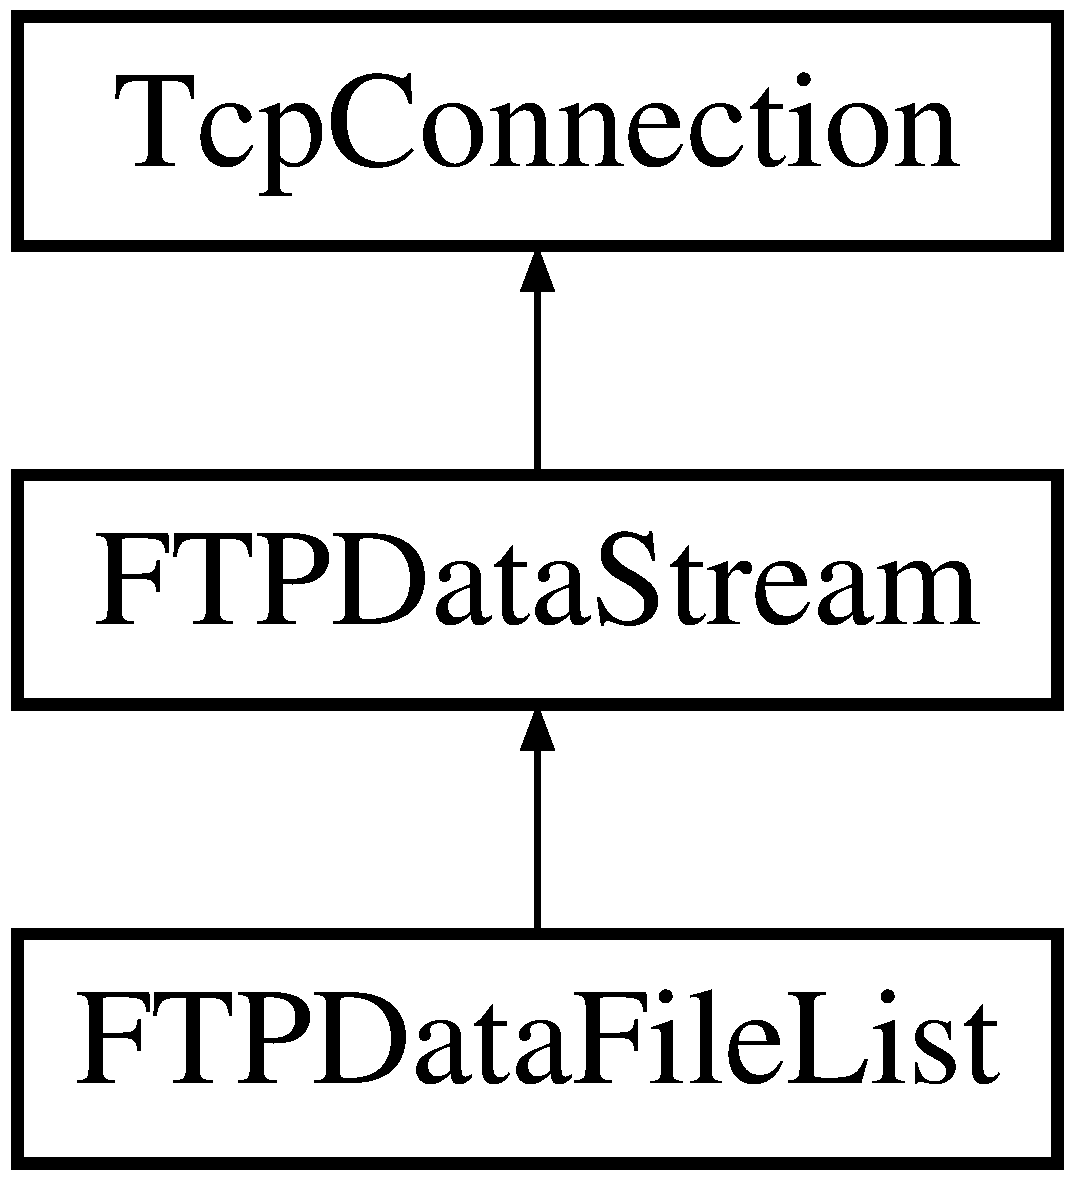
\includegraphics[height=3.000000cm]{class_f_t_p_data_file_list}
\end{center}
\end{figure}
\subsection*{Public Member Functions}
\begin{DoxyCompactItemize}
\item 
\hypertarget{class_f_t_p_data_file_list_a36822a3b9d921cd9a0debb4a6d15f24e}{}{\bfseries F\+T\+P\+Data\+File\+List} (\hyperlink{class_f_t_p_server_connection}{F\+T\+P\+Server\+Connection} $\ast$connection)\label{class_f_t_p_data_file_list_a36822a3b9d921cd9a0debb4a6d15f24e}

\item 
\hypertarget{class_f_t_p_data_file_list_a2883090e36e8560d9100cd48f1ab2f03}{}virtual void {\bfseries transfer\+Data} (Tcp\+Connection\+Event source\+Event)\label{class_f_t_p_data_file_list_a2883090e36e8560d9100cd48f1ab2f03}

\end{DoxyCompactItemize}
\subsection*{Additional Inherited Members}


The documentation for this class was generated from the following file\+:\begin{DoxyCompactItemize}
\item 
Sming\+Core/\+Network/F\+T\+P\+Server\+Connection.\+cpp\end{DoxyCompactItemize}

\hypertarget{class_f_t_p_data_retrieve}{}\section{F\+T\+P\+Data\+Retrieve Class Reference}
\label{class_f_t_p_data_retrieve}\index{F\+T\+P\+Data\+Retrieve@{F\+T\+P\+Data\+Retrieve}}
Inheritance diagram for F\+T\+P\+Data\+Retrieve\+:\begin{figure}[H]
\begin{center}
\leavevmode
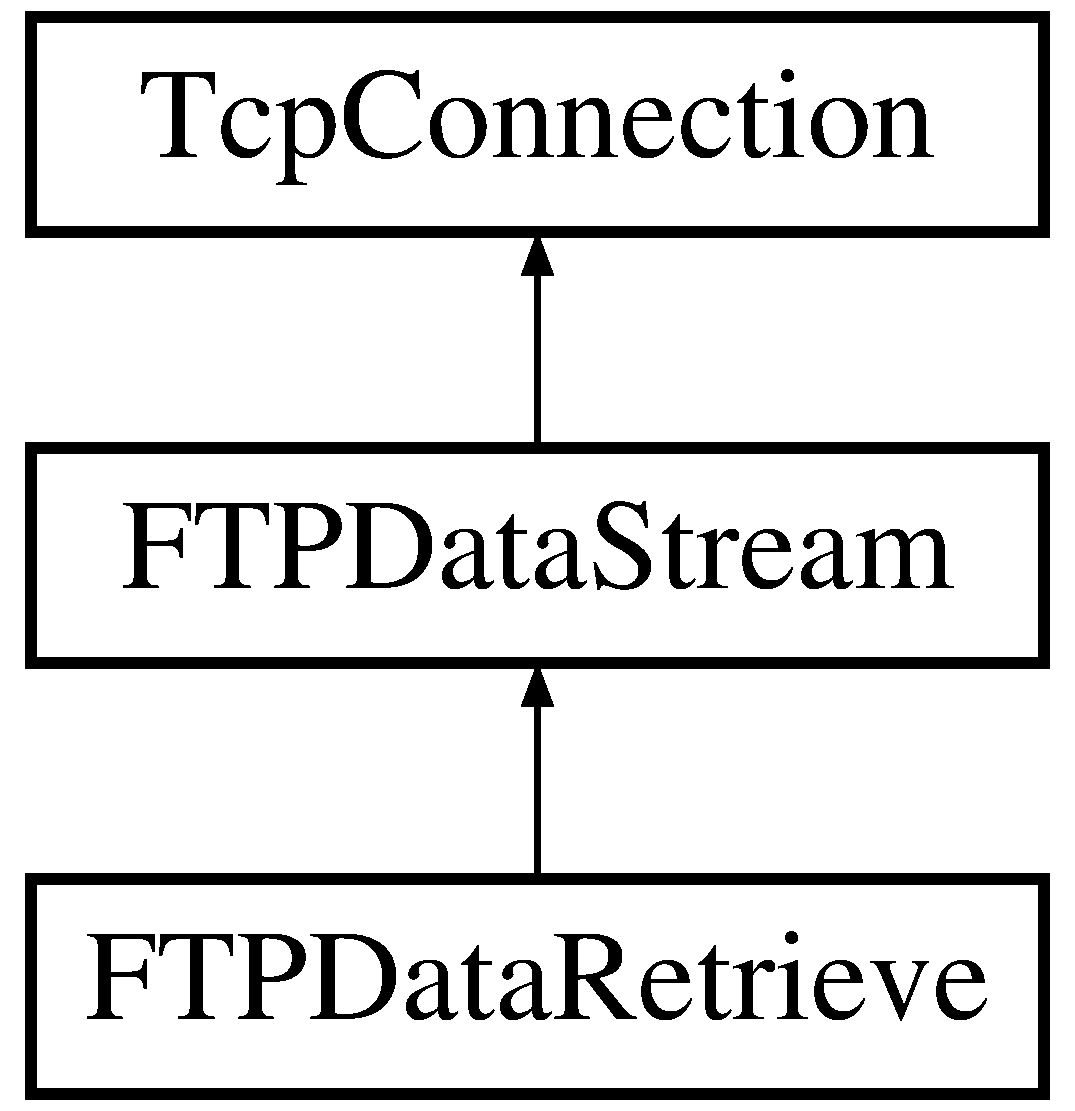
\includegraphics[height=3.000000cm]{class_f_t_p_data_retrieve}
\end{center}
\end{figure}
\subsection*{Public Member Functions}
\begin{DoxyCompactItemize}
\item 
\hypertarget{class_f_t_p_data_retrieve_a9d886ba51a823e38b1bb7b68ef53b93b}{}{\bfseries F\+T\+P\+Data\+Retrieve} (\hyperlink{class_f_t_p_server_connection}{F\+T\+P\+Server\+Connection} $\ast$connection, String file\+Name)\label{class_f_t_p_data_retrieve_a9d886ba51a823e38b1bb7b68ef53b93b}

\item 
\hypertarget{class_f_t_p_data_retrieve_a6dfb5d32a7ef8a463f0a650ae04154f9}{}virtual void {\bfseries transfer\+Data} (Tcp\+Connection\+Event source\+Event)\label{class_f_t_p_data_retrieve_a6dfb5d32a7ef8a463f0a650ae04154f9}

\end{DoxyCompactItemize}
\subsection*{Additional Inherited Members}


The documentation for this class was generated from the following file\+:\begin{DoxyCompactItemize}
\item 
Sming\+Core/\+Network/F\+T\+P\+Server\+Connection.\+cpp\end{DoxyCompactItemize}

\hypertarget{class_f_t_p_data_store}{}\section{F\+T\+P\+Data\+Store Class Reference}
\label{class_f_t_p_data_store}\index{F\+T\+P\+Data\+Store@{F\+T\+P\+Data\+Store}}
Inheritance diagram for F\+T\+P\+Data\+Store\+:\begin{figure}[H]
\begin{center}
\leavevmode
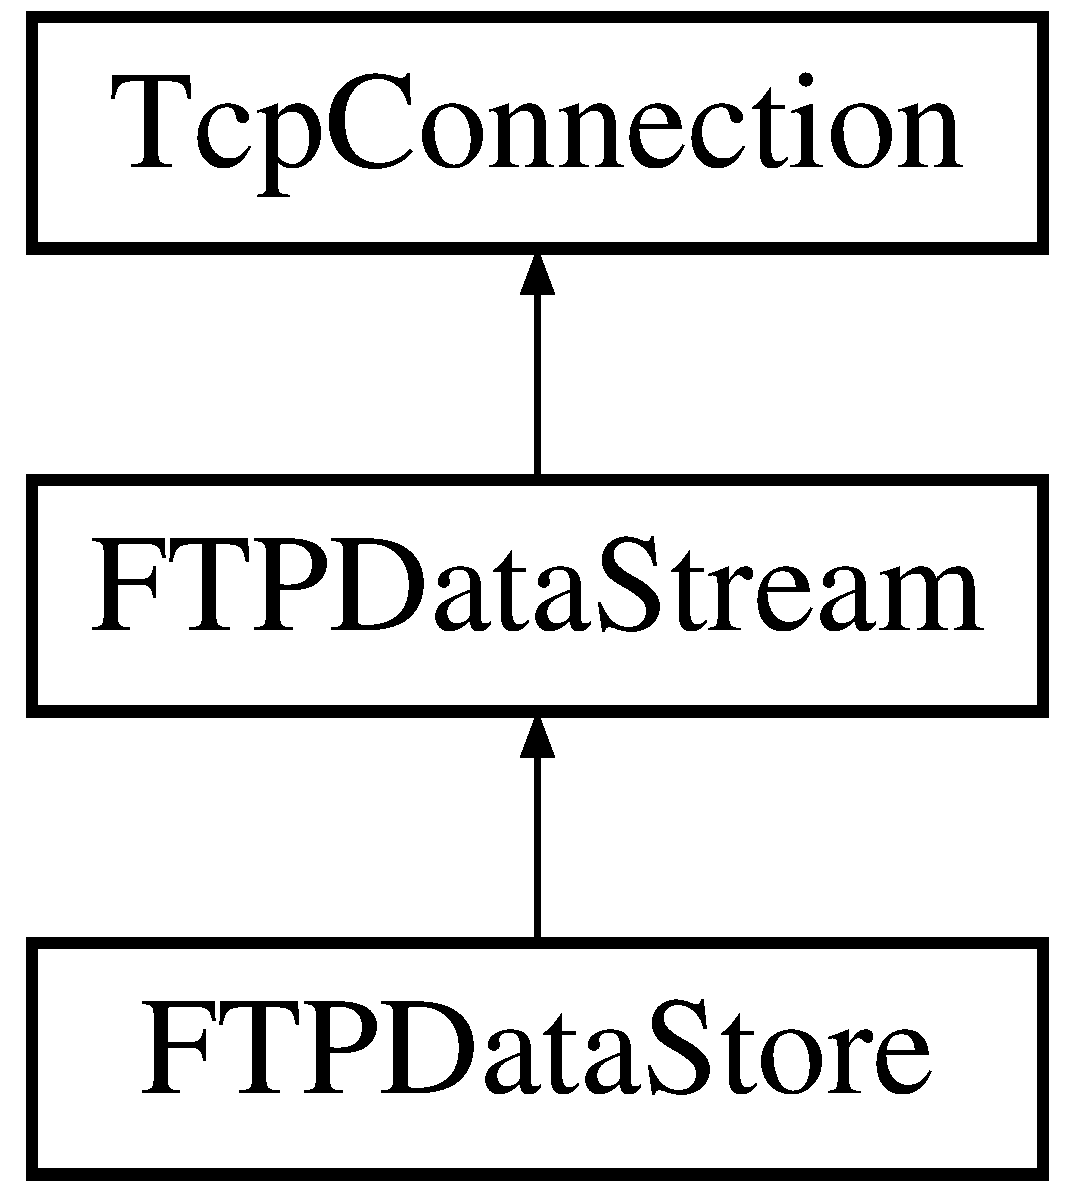
\includegraphics[height=3.000000cm]{class_f_t_p_data_store}
\end{center}
\end{figure}
\subsection*{Public Member Functions}
\begin{DoxyCompactItemize}
\item 
\hypertarget{class_f_t_p_data_store_a17182d9c40530b2a97f08751d8c13a75}{}{\bfseries F\+T\+P\+Data\+Store} (\hyperlink{class_f_t_p_server_connection}{F\+T\+P\+Server\+Connection} $\ast$connection, String file\+Name)\label{class_f_t_p_data_store_a17182d9c40530b2a97f08751d8c13a75}

\item 
\hypertarget{class_f_t_p_data_store_a34b216c8bbde46d3415a82b2dd5b066d}{}virtual err\+\_\+t {\bfseries on\+Receive} (\hyperlink{structpbuf}{pbuf} $\ast$buf)\label{class_f_t_p_data_store_a34b216c8bbde46d3415a82b2dd5b066d}

\end{DoxyCompactItemize}
\subsection*{Additional Inherited Members}


The documentation for this class was generated from the following file\+:\begin{DoxyCompactItemize}
\item 
Sming\+Core/\+Network/F\+T\+P\+Server\+Connection.\+cpp\end{DoxyCompactItemize}

\hypertarget{class_f_t_p_data_stream}{}\section{F\+T\+P\+Data\+Stream Class Reference}
\label{class_f_t_p_data_stream}\index{F\+T\+P\+Data\+Stream@{F\+T\+P\+Data\+Stream}}
Inheritance diagram for F\+T\+P\+Data\+Stream\+:\begin{figure}[H]
\begin{center}
\leavevmode
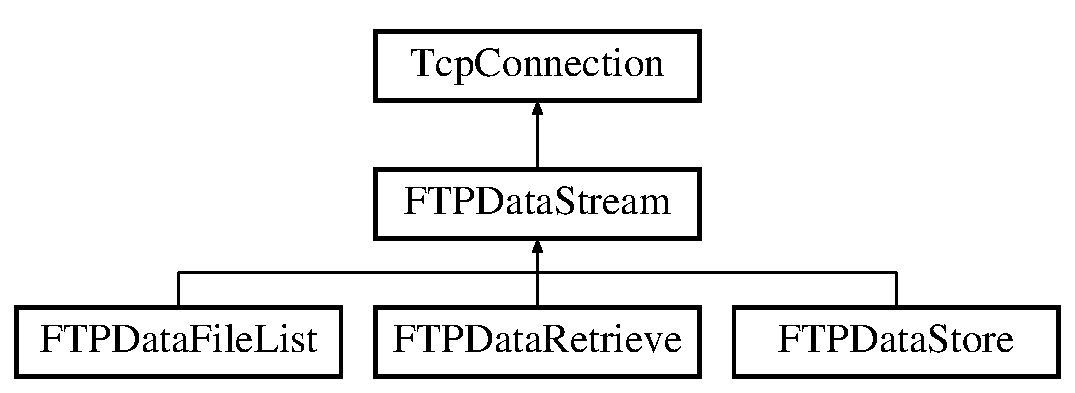
\includegraphics[height=3.000000cm]{class_f_t_p_data_stream}
\end{center}
\end{figure}
\subsection*{Public Member Functions}
\begin{DoxyCompactItemize}
\item 
\hypertarget{class_f_t_p_data_stream_a2af1acb58e2cf042ac8fc07e8ccdc3a3}{}{\bfseries F\+T\+P\+Data\+Stream} (\hyperlink{class_f_t_p_server_connection}{F\+T\+P\+Server\+Connection} $\ast$connection)\label{class_f_t_p_data_stream_a2af1acb58e2cf042ac8fc07e8ccdc3a3}

\item 
\hypertarget{class_f_t_p_data_stream_aca2f90b7902043fcb71bc4d959732387}{}virtual err\+\_\+t {\bfseries on\+Connected} (err\+\_\+t err)\label{class_f_t_p_data_stream_aca2f90b7902043fcb71bc4d959732387}

\item 
\hypertarget{class_f_t_p_data_stream_a8a6ea4976b357a6307c4fba634a75db9}{}virtual err\+\_\+t {\bfseries on\+Sent} (uint16\+\_\+t len)\label{class_f_t_p_data_stream_a8a6ea4976b357a6307c4fba634a75db9}

\item 
\hypertarget{class_f_t_p_data_stream_a9cbc0ceadf3730c1164afed24d84f5f8}{}void {\bfseries finish\+Transfer} ()\label{class_f_t_p_data_stream_a9cbc0ceadf3730c1164afed24d84f5f8}

\item 
\hypertarget{class_f_t_p_data_stream_a73a91d01d206fc8ffc78228368b9d2ac}{}void {\bfseries response} (int code, String text=\char`\"{}\char`\"{})\label{class_f_t_p_data_stream_a73a91d01d206fc8ffc78228368b9d2ac}

\item 
\hypertarget{class_f_t_p_data_stream_a8da4f750cf0b17429e8d730cdd676c8e}{}int {\bfseries write} (const char $\ast$data, int len, uint8\+\_\+t apiflags=0)\label{class_f_t_p_data_stream_a8da4f750cf0b17429e8d730cdd676c8e}

\item 
\hypertarget{class_f_t_p_data_stream_a52fd64cf6ecd66115e52e790bdcf2dd7}{}virtual void {\bfseries on\+Ready\+To\+Send\+Data} (Tcp\+Connection\+Event source\+Event)\label{class_f_t_p_data_stream_a52fd64cf6ecd66115e52e790bdcf2dd7}

\item 
\hypertarget{class_f_t_p_data_stream_ac10b635d64be2b913bc8a3fbe6631271}{}virtual void {\bfseries transfer\+Data} (Tcp\+Connection\+Event source\+Event)\label{class_f_t_p_data_stream_ac10b635d64be2b913bc8a3fbe6631271}

\end{DoxyCompactItemize}
\subsection*{Protected Attributes}
\begin{DoxyCompactItemize}
\item 
\hypertarget{class_f_t_p_data_stream_a6db9ff53eb8823e1e00892cd5da9fbd4}{}\hyperlink{class_f_t_p_server_connection}{F\+T\+P\+Server\+Connection} $\ast$ {\bfseries parent}\label{class_f_t_p_data_stream_a6db9ff53eb8823e1e00892cd5da9fbd4}

\item 
\hypertarget{class_f_t_p_data_stream_aad73d06e1fb6b7191a7bff8e28c6f216}{}bool {\bfseries completed}\label{class_f_t_p_data_stream_aad73d06e1fb6b7191a7bff8e28c6f216}

\item 
\hypertarget{class_f_t_p_data_stream_a0cd2d52a8205a08bb3a5aadc634c3254}{}int {\bfseries written}\label{class_f_t_p_data_stream_a0cd2d52a8205a08bb3a5aadc634c3254}

\item 
\hypertarget{class_f_t_p_data_stream_a16f4c6b5fa1bce3a838a88858dd36b2f}{}int {\bfseries sent}\label{class_f_t_p_data_stream_a16f4c6b5fa1bce3a838a88858dd36b2f}

\end{DoxyCompactItemize}
\subsection*{Additional Inherited Members}


The documentation for this class was generated from the following file\+:\begin{DoxyCompactItemize}
\item 
Sming\+Core/\+Network/F\+T\+P\+Server\+Connection.\+cpp\end{DoxyCompactItemize}

\hypertarget{class_f_t_p_server}{}\section{F\+T\+P\+Server Class Reference}
\label{class_f_t_p_server}\index{F\+T\+P\+Server@{F\+T\+P\+Server}}
Inheritance diagram for F\+T\+P\+Server\+:\begin{figure}[H]
\begin{center}
\leavevmode
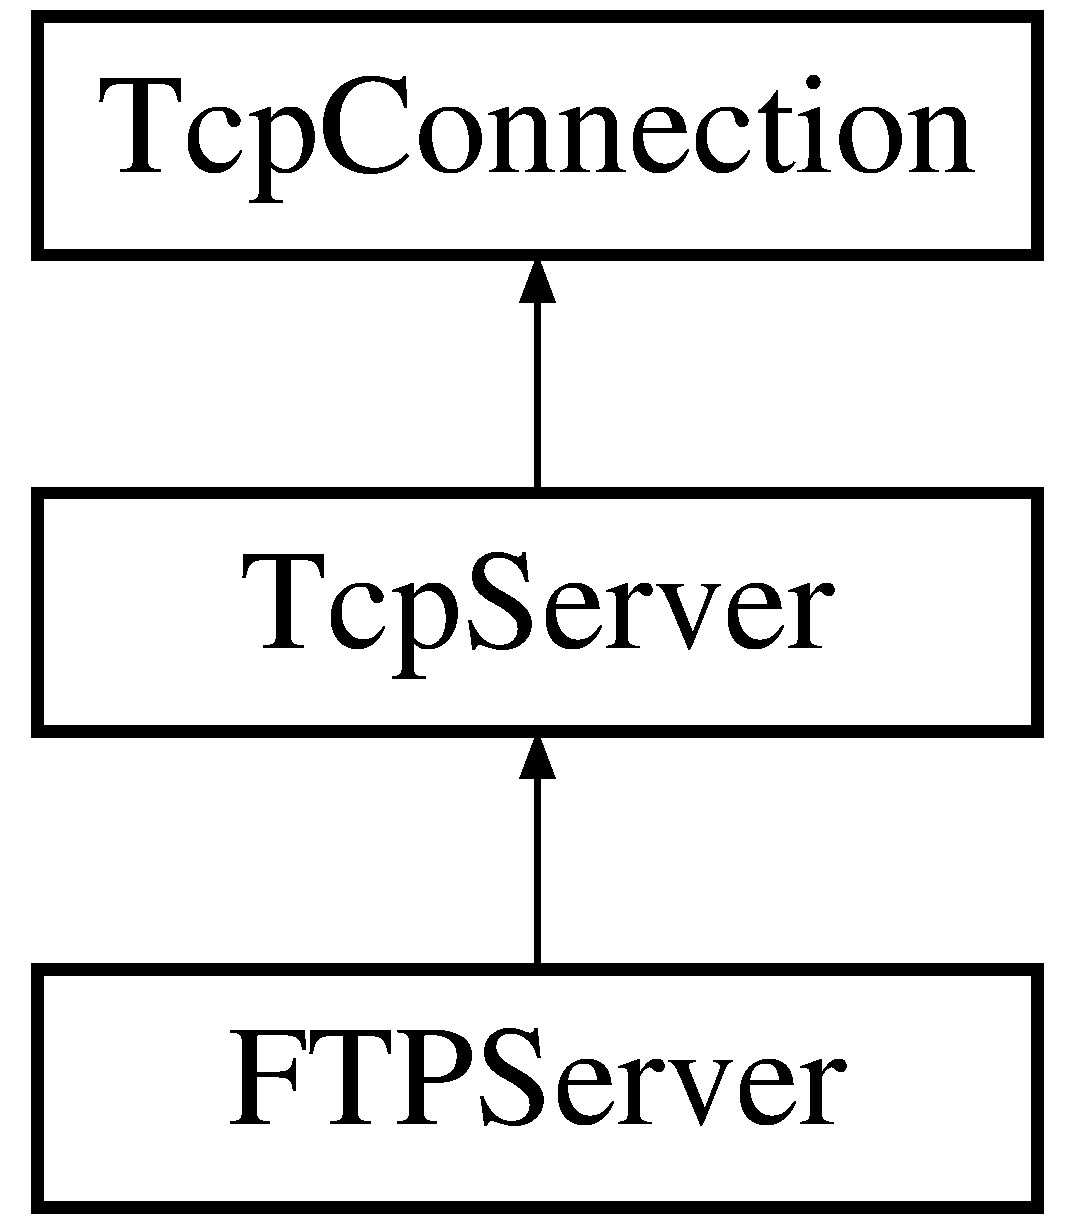
\includegraphics[height=3.000000cm]{class_f_t_p_server}
\end{center}
\end{figure}
\subsection*{Public Member Functions}
\begin{DoxyCompactItemize}
\item 
\hypertarget{class_f_t_p_server_adddb840204f296775d059075c440d9f9}{}void {\bfseries add\+User} (String login, String pass)\label{class_f_t_p_server_adddb840204f296775d059075c440d9f9}

\item 
\hypertarget{class_f_t_p_server_a427ae5840b2491164bb3e92099ee469e}{}bool {\bfseries check\+User} (String login, String pass)\label{class_f_t_p_server_a427ae5840b2491164bb3e92099ee469e}

\end{DoxyCompactItemize}
\subsection*{Protected Member Functions}
\begin{DoxyCompactItemize}
\item 
\hypertarget{class_f_t_p_server_a092faf3fadd29a175b7df817a1919099}{}virtual \hyperlink{class_tcp_connection}{Tcp\+Connection} $\ast$ {\bfseries create\+Client} (tcp\+\_\+pcb $\ast$client\+Tcp)\label{class_f_t_p_server_a092faf3fadd29a175b7df817a1919099}

\item 
\hypertarget{class_f_t_p_server_afd4dd8a2a6f63cec55aeeac0fbc1a4ac}{}virtual bool {\bfseries on\+Command} (String cmd, String data, \hyperlink{class_f_t_p_server_connection}{F\+T\+P\+Server\+Connection} \&connection)\label{class_f_t_p_server_afd4dd8a2a6f63cec55aeeac0fbc1a4ac}

\end{DoxyCompactItemize}
\subsection*{Friends}
\begin{DoxyCompactItemize}
\item 
\hypertarget{class_f_t_p_server_a488b1abba79677c92b11c9b75f74bb53}{}class {\bfseries F\+T\+P\+Server\+Connection}\label{class_f_t_p_server_a488b1abba79677c92b11c9b75f74bb53}

\end{DoxyCompactItemize}
\subsection*{Additional Inherited Members}


The documentation for this class was generated from the following files\+:\begin{DoxyCompactItemize}
\item 
Sming\+Core/\+Network/F\+T\+P\+Server.\+h\item 
Sming\+Core/\+Network/F\+T\+P\+Server.\+cpp\end{DoxyCompactItemize}

\hypertarget{class_f_t_p_server_connection}{}\section{F\+T\+P\+Server\+Connection Class Reference}
\label{class_f_t_p_server_connection}\index{F\+T\+P\+Server\+Connection@{F\+T\+P\+Server\+Connection}}
Inheritance diagram for F\+T\+P\+Server\+Connection\+:\begin{figure}[H]
\begin{center}
\leavevmode
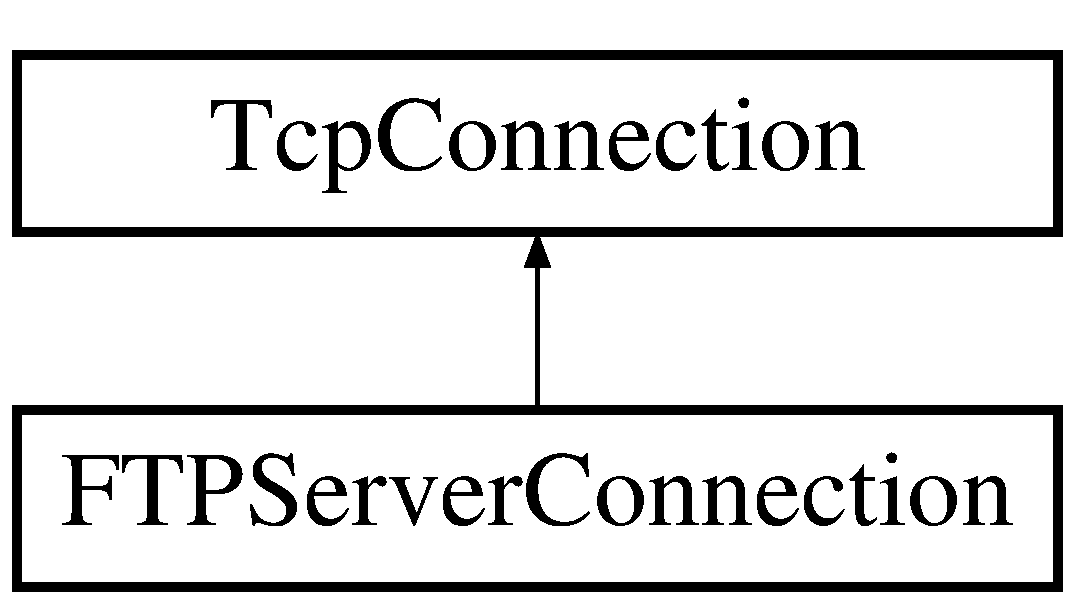
\includegraphics[height=2.000000cm]{class_f_t_p_server_connection}
\end{center}
\end{figure}
\subsection*{Public Member Functions}
\begin{DoxyCompactItemize}
\item 
\hypertarget{class_f_t_p_server_connection_aacecab901ba08f31707c8b151b39aa0b}{}{\bfseries F\+T\+P\+Server\+Connection} (\hyperlink{class_f_t_p_server}{F\+T\+P\+Server} $\ast$parent\+Server, tcp\+\_\+pcb $\ast$client\+Tcp)\label{class_f_t_p_server_connection_aacecab901ba08f31707c8b151b39aa0b}

\item 
\hypertarget{class_f_t_p_server_connection_a40eb5a9cd076787f023ad736e55b1386}{}virtual err\+\_\+t {\bfseries on\+Receive} (\hyperlink{structpbuf}{pbuf} $\ast$buf)\label{class_f_t_p_server_connection_a40eb5a9cd076787f023ad736e55b1386}

\item 
\hypertarget{class_f_t_p_server_connection_ad47f32a37c2cf7bb69082ab1b217955d}{}virtual err\+\_\+t {\bfseries on\+Sent} (uint16\+\_\+t len)\label{class_f_t_p_server_connection_ad47f32a37c2cf7bb69082ab1b217955d}

\item 
\hypertarget{class_f_t_p_server_connection_a3352742c3dff1a7405703bb04bcce16c}{}virtual void {\bfseries on\+Ready\+To\+Send\+Data} (Tcp\+Connection\+Event source\+Event)\label{class_f_t_p_server_connection_a3352742c3dff1a7405703bb04bcce16c}

\item 
\hypertarget{class_f_t_p_server_connection_a5d5d227c7a274938e303fee4df39c53c}{}void {\bfseries data\+Transfer\+Finished} (\hyperlink{class_tcp_connection}{Tcp\+Connection} $\ast$connection)\label{class_f_t_p_server_connection_a5d5d227c7a274938e303fee4df39c53c}

\end{DoxyCompactItemize}
\subsection*{Protected Member Functions}
\begin{DoxyCompactItemize}
\item 
\hypertarget{class_f_t_p_server_connection_ac2db42bde1c485cb649638eeeba45b55}{}virtual void {\bfseries on\+Command} (String cmd, String data)\label{class_f_t_p_server_connection_ac2db42bde1c485cb649638eeeba45b55}

\item 
\hypertarget{class_f_t_p_server_connection_a0e10956fe9b5eced5d1531c85ed2092c}{}virtual void {\bfseries response} (int code, String text=\char`\"{}\char`\"{})\label{class_f_t_p_server_connection_a0e10956fe9b5eced5d1531c85ed2092c}

\item 
\hypertarget{class_f_t_p_server_connection_a8e537ef40a67def74890e6b0d7e1de3d}{}int {\bfseries get\+Splitter\+Pos} (String data, char splitter, uint8\+\_\+t number)\label{class_f_t_p_server_connection_a8e537ef40a67def74890e6b0d7e1de3d}

\item 
\hypertarget{class_f_t_p_server_connection_a93e4df7c53271118e3975b9f2ee4ba66}{}String {\bfseries make\+File\+Name} (String name, bool short\+It)\label{class_f_t_p_server_connection_a93e4df7c53271118e3975b9f2ee4ba66}

\item 
\hypertarget{class_f_t_p_server_connection_a60d9eea49392714f23d28c88a55c3e4b}{}void {\bfseries cmd\+Port} (const String \&data)\label{class_f_t_p_server_connection_a60d9eea49392714f23d28c88a55c3e4b}

\item 
\hypertarget{class_f_t_p_server_connection_a437c82fc427d5463cc3bc13261a71317}{}void {\bfseries create\+Data\+Connection} (\hyperlink{class_tcp_connection}{Tcp\+Connection} $\ast$connection)\label{class_f_t_p_server_connection_a437c82fc427d5463cc3bc13261a71317}

\item 
\hypertarget{class_f_t_p_server_connection_a92fc4d82fc9c5b3cc3b65adae26d2eae}{}bool {\bfseries is\+Can\+Transfer} ()\label{class_f_t_p_server_connection_a92fc4d82fc9c5b3cc3b65adae26d2eae}

\end{DoxyCompactItemize}
\subsection*{Friends}
\begin{DoxyCompactItemize}
\item 
\hypertarget{class_f_t_p_server_connection_a99e599a35280ac84d2e1f25cafa8d2aa}{}class {\bfseries F\+T\+P\+Data\+Stream}\label{class_f_t_p_server_connection_a99e599a35280ac84d2e1f25cafa8d2aa}

\item 
\hypertarget{class_f_t_p_server_connection_a30283ec79f994d5512e92217a7c033e8}{}class {\bfseries F\+T\+P\+Server}\label{class_f_t_p_server_connection_a30283ec79f994d5512e92217a7c033e8}

\end{DoxyCompactItemize}
\subsection*{Additional Inherited Members}


The documentation for this class was generated from the following files\+:\begin{DoxyCompactItemize}
\item 
Sming\+Core/\+Network/F\+T\+P\+Server\+Connection.\+h\item 
Sming\+Core/\+Network/F\+T\+P\+Server\+Connection.\+cpp\end{DoxyCompactItemize}

\hypertarget{class_function_caller}{}\section{Function\+Caller$<$ Method\+Declaration, Return\+Type, Params\+List $>$ Class Template Reference}
\label{class_function_caller}\index{Function\+Caller$<$ Method\+Declaration, Return\+Type, Params\+List $>$@{Function\+Caller$<$ Method\+Declaration, Return\+Type, Params\+List $>$}}
Inheritance diagram for Function\+Caller$<$ Method\+Declaration, Return\+Type, Params\+List $>$\+:\begin{figure}[H]
\begin{center}
\leavevmode
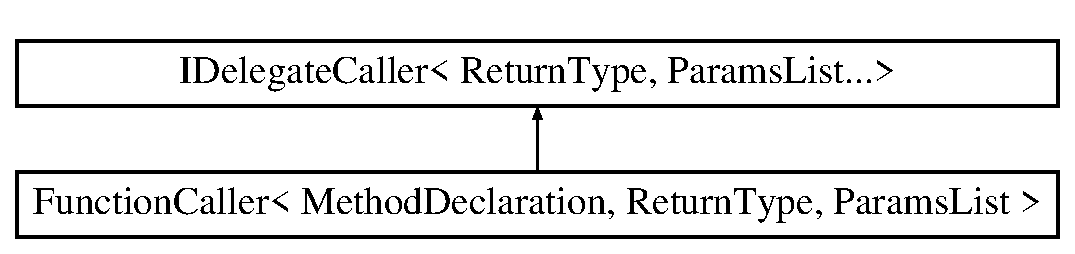
\includegraphics[height=2.000000cm]{class_function_caller}
\end{center}
\end{figure}
\subsection*{Public Member Functions}
\begin{DoxyCompactItemize}
\item 
\hypertarget{class_function_caller_a57489bd2e7cd5a17d454c5d3ab98cecc}{}{\bfseries Function\+Caller} (Method\+Declaration m)\label{class_function_caller_a57489bd2e7cd5a17d454c5d3ab98cecc}

\item 
\hypertarget{class_function_caller_a129be846b2a8a64fb7816a0f2cf8eb94}{}Return\+Type {\bfseries invoke} (Params\+List...\+args)\label{class_function_caller_a129be846b2a8a64fb7816a0f2cf8eb94}

\end{DoxyCompactItemize}


The documentation for this class was generated from the following file\+:\begin{DoxyCompactItemize}
\item 
Sming\+Core/Delegate.\+h\end{DoxyCompactItemize}

\hypertarget{class_hardware_serial}{}\section{Hardware\+Serial Class Reference}
\label{class_hardware_serial}\index{Hardware\+Serial@{Hardware\+Serial}}
Inheritance diagram for Hardware\+Serial\+:\begin{figure}[H]
\begin{center}
\leavevmode
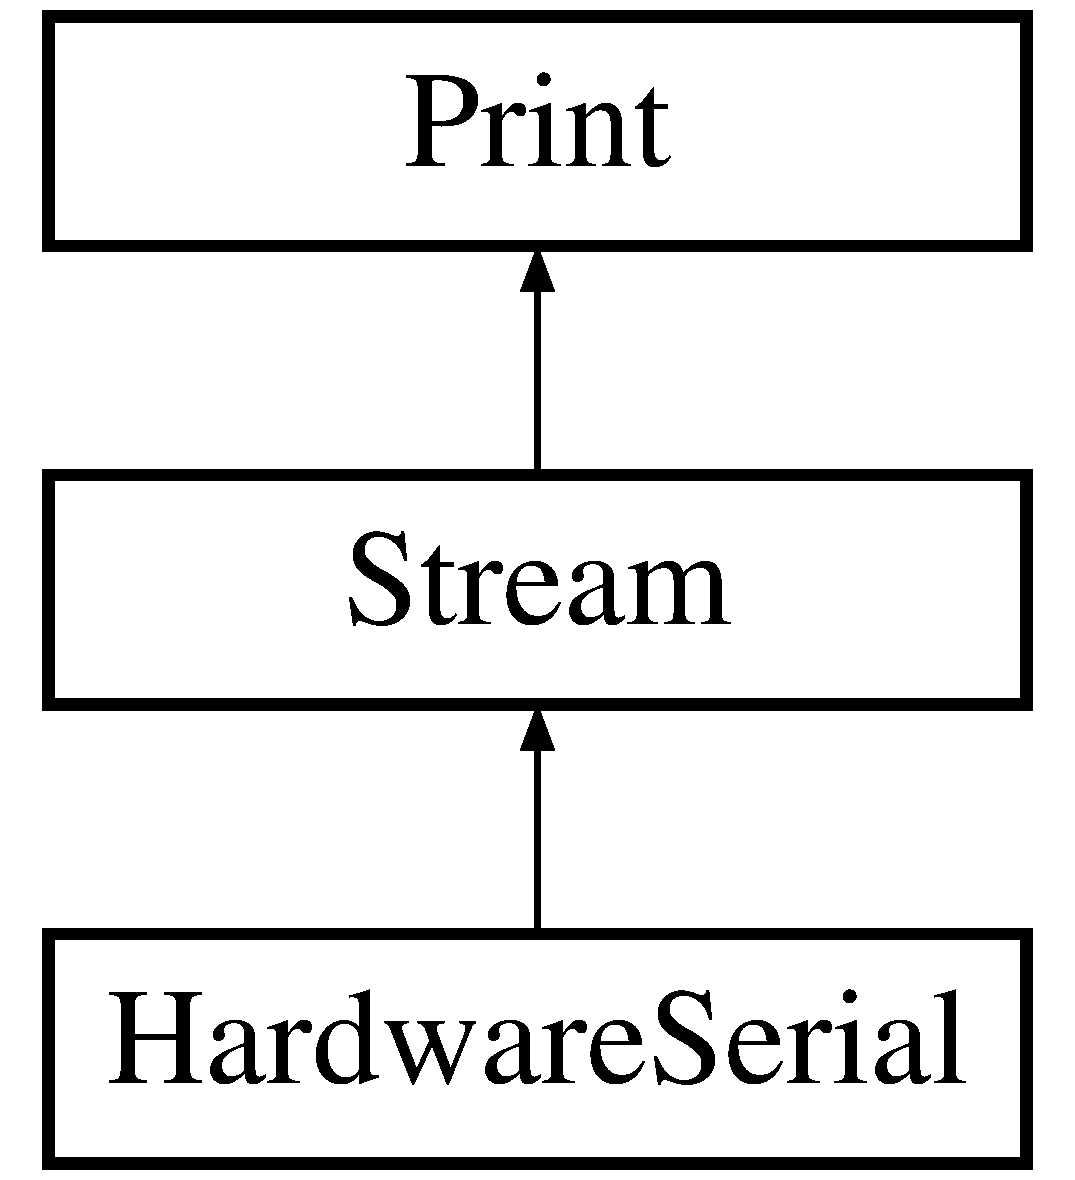
\includegraphics[height=3.000000cm]{class_hardware_serial}
\end{center}
\end{figure}
\subsection*{Public Member Functions}
\begin{DoxyCompactItemize}
\item 
\hypertarget{class_hardware_serial_a3227f49b50f3f6a0d3e1c7641e82697b}{}{\bfseries Hardware\+Serial} (const int uart\+Port)\label{class_hardware_serial_a3227f49b50f3f6a0d3e1c7641e82697b}

\item 
\hypertarget{class_hardware_serial_ad10f3f07a59e390851b4ed47b8991d39}{}void {\bfseries begin} (const uint32\+\_\+t baud=9600)\label{class_hardware_serial_ad10f3f07a59e390851b4ed47b8991d39}

\item 
\hypertarget{class_hardware_serial_a609a8c9b978ce60334e93afc8625a91e}{}int {\bfseries available} ()\label{class_hardware_serial_a609a8c9b978ce60334e93afc8625a91e}

\item 
\hypertarget{class_hardware_serial_a3a60d321a0c62fa16a4e41dffe7e0242}{}int {\bfseries read} ()\label{class_hardware_serial_a3a60d321a0c62fa16a4e41dffe7e0242}

\item 
\hypertarget{class_hardware_serial_a7a340ec4cf7c689e95964b58c5bbc7c3}{}int {\bfseries read\+Memory\+Block} (char $\ast$buf, int max\+\_\+len)\label{class_hardware_serial_a7a340ec4cf7c689e95964b58c5bbc7c3}

\item 
\hypertarget{class_hardware_serial_a7acdf929737d21dc2ea9000d478d1fbb}{}int {\bfseries peek} ()\label{class_hardware_serial_a7acdf929737d21dc2ea9000d478d1fbb}

\item 
\hypertarget{class_hardware_serial_af12cc7f03315df841905003d728d9b87}{}void {\bfseries flush} ()\label{class_hardware_serial_af12cc7f03315df841905003d728d9b87}

\item 
\hypertarget{class_hardware_serial_a0115a99310d2c24205fdc13d692ad4be}{}size\+\_\+t {\bfseries write} (uint8\+\_\+t one\+Char)\label{class_hardware_serial_a0115a99310d2c24205fdc13d692ad4be}

\item 
\hypertarget{class_hardware_serial_a1365b152178ff99287c1e700b593a0e0}{}void {\bfseries system\+Debug\+Output} (bool enabled)\label{class_hardware_serial_a1365b152178ff99287c1e700b593a0e0}

\end{DoxyCompactItemize}
\subsection*{Static Public Member Functions}
\begin{DoxyCompactItemize}
\item 
\hypertarget{class_hardware_serial_a71a922d109d82c8e2a657641623ee255}{}static void I\+R\+A\+M\+\_\+\+A\+T\+T\+R {\bfseries uart0\+\_\+rx\+\_\+intr\+\_\+handler} (void $\ast$para)\label{class_hardware_serial_a71a922d109d82c8e2a657641623ee255}

\end{DoxyCompactItemize}
\subsection*{Additional Inherited Members}


The documentation for this class was generated from the following files\+:\begin{DoxyCompactItemize}
\item 
Sming\+Core/Hardware\+Serial.\+h\item 
Sming\+Core/Hardware\+Serial.\+cpp\end{DoxyCompactItemize}

\hypertarget{class_hash_map}{}\section{Hash\+Map$<$ K, V $>$ Class Template Reference}
\label{class_hash_map}\index{Hash\+Map$<$ K, V $>$@{Hash\+Map$<$ K, V $>$}}
\subsection*{Public Types}
\begin{DoxyCompactItemize}
\item 
\hypertarget{class_hash_map_ad069a14b9dbe415654f0a75d2f75903a}{}typedef bool($\ast$ {\bfseries comparator}) (K, K)\label{class_hash_map_ad069a14b9dbe415654f0a75d2f75903a}

\end{DoxyCompactItemize}
\subsection*{Public Member Functions}
\begin{DoxyCompactItemize}
\item 
\hypertarget{class_hash_map_a0b42a9214e1d10a9d9ca3631108136c2}{}{\bfseries Hash\+Map} (comparator compare=0)\label{class_hash_map_a0b42a9214e1d10a9d9ca3631108136c2}

\item 
\hypertarget{class_hash_map_a7d6a983573e5e82d11cb5025ef647766}{}unsigned int {\bfseries count} () const \label{class_hash_map_a7d6a983573e5e82d11cb5025ef647766}

\item 
\hypertarget{class_hash_map_a5070fc6cee92fec011d76f7031a6b274}{}K {\bfseries key\+At} (unsigned int idx) const \label{class_hash_map_a5070fc6cee92fec011d76f7031a6b274}

\item 
\hypertarget{class_hash_map_aec6f25ebf692fad067a29d275aa9baf8}{}V {\bfseries value\+At} (unsigned int idx) const \label{class_hash_map_aec6f25ebf692fad067a29d275aa9baf8}

\item 
\hypertarget{class_hash_map_a42b684810281db5ed6c7a5ba6a925424}{}const V \& {\bfseries operator\mbox{[}$\,$\mbox{]}} (const K key) const \label{class_hash_map_a42b684810281db5ed6c7a5ba6a925424}

\item 
\hypertarget{class_hash_map_a24680bf5f24f1a562203be77f384ccc0}{}V \& {\bfseries operator\mbox{[}$\,$\mbox{]}} (const K key)\label{class_hash_map_a24680bf5f24f1a562203be77f384ccc0}

\item 
\hypertarget{class_hash_map_a8a1a7a52d83d17407a3fdca25d99df5f}{}void {\bfseries allocate} (int new\+Size)\label{class_hash_map_a8a1a7a52d83d17407a3fdca25d99df5f}

\item 
\hypertarget{class_hash_map_a9f3ea677a801d751ca58bc4315d4d4d8}{}unsigned int {\bfseries index\+Of} (K key) const \label{class_hash_map_a9f3ea677a801d751ca58bc4315d4d4d8}

\item 
\hypertarget{class_hash_map_a5d2ae7130ed966f4538f3d23e544e747}{}bool {\bfseries contains} (K key) const \label{class_hash_map_a5d2ae7130ed966f4538f3d23e544e747}

\item 
\hypertarget{class_hash_map_a78fdd35d77ed013c141a09138339455d}{}void {\bfseries remove} (K key)\label{class_hash_map_a78fdd35d77ed013c141a09138339455d}

\item 
\hypertarget{class_hash_map_ac5a8399ea019f8023bdad58a5c71f129}{}void {\bfseries set\+Multiple} (const \hyperlink{class_hash_map}{Hash\+Map}$<$ K, V $>$ \&map)\label{class_hash_map_ac5a8399ea019f8023bdad58a5c71f129}

\item 
\hypertarget{class_hash_map_acb737f38a458ac98ad1c01400ea8b572}{}void {\bfseries set\+Null\+Value} (V nullv)\label{class_hash_map_acb737f38a458ac98ad1c01400ea8b572}

\end{DoxyCompactItemize}
\subsection*{Protected Attributes}
\begin{DoxyCompactItemize}
\item 
\hypertarget{class_hash_map_a655e048c02f3bdbc0c3f300d5a73ab88}{}K $\ast$$\ast$ {\bfseries keys}\label{class_hash_map_a655e048c02f3bdbc0c3f300d5a73ab88}

\item 
\hypertarget{class_hash_map_a5811d197090726d10507a6189ce18873}{}V $\ast$$\ast$ {\bfseries values}\label{class_hash_map_a5811d197090726d10507a6189ce18873}

\item 
\hypertarget{class_hash_map_af2b76f3bd067749d61fd1ffd8eeee4a5}{}V {\bfseries nil}\label{class_hash_map_af2b76f3bd067749d61fd1ffd8eeee4a5}

\item 
\hypertarget{class_hash_map_aa2a734a0037110e66fc763a5be567bfa}{}int16\+\_\+t {\bfseries current\+Index}\label{class_hash_map_aa2a734a0037110e66fc763a5be567bfa}

\item 
\hypertarget{class_hash_map_a485fb8ca016d231e33181dc80a0ac796}{}int16\+\_\+t {\bfseries size}\label{class_hash_map_a485fb8ca016d231e33181dc80a0ac796}

\item 
\hypertarget{class_hash_map_aa81d7fa34e94848ae00b257e5f74cd3d}{}comparator {\bfseries cb\+\_\+comparator}\label{class_hash_map_aa81d7fa34e94848ae00b257e5f74cd3d}

\end{DoxyCompactItemize}


The documentation for this class was generated from the following file\+:\begin{DoxyCompactItemize}
\item 
Wiring/W\+Hash\+Map.\+h\end{DoxyCompactItemize}

\hypertarget{class_h_m_c5883_l}{}\section{H\+M\+C5883\+L Class Reference}
\label{class_h_m_c5883_l}\index{H\+M\+C5883\+L@{H\+M\+C5883\+L}}
\subsection*{Public Member Functions}
\begin{DoxyCompactItemize}
\item 
\hyperlink{class_h_m_c5883_l_ab552ed5dd985c500aa37ac11f9ed3eed}{H\+M\+C5883\+L} ()
\item 
\hyperlink{class_h_m_c5883_l_ad7dd693f11a1486efb3ecd7d3d5158b6}{H\+M\+C5883\+L} (uint8\+\_\+t address)
\item 
void \hyperlink{class_h_m_c5883_l_a6e895366c47f22ab9dbe2750f2302dc4}{initialize} ()
\item 
bool \hyperlink{class_h_m_c5883_l_acfa47db9eccdf7ac120935de8a123f33}{test\+Connection} ()
\item 
uint8\+\_\+t \hyperlink{class_h_m_c5883_l_a99c7262f906b7bd4b0deb4e94857dfd9}{get\+Sample\+Averaging} ()
\item 
void \hyperlink{class_h_m_c5883_l_a9bf281a4dcf8f21f9a64624f835b8974}{set\+Sample\+Averaging} (uint8\+\_\+t averaging)
\item 
uint8\+\_\+t \hyperlink{class_h_m_c5883_l_aabc0bc9aca80ba60edb73a3a79a3591a}{get\+Data\+Rate} ()
\item 
void \hyperlink{class_h_m_c5883_l_a2a13729786821e826448fac7ee43ad9e}{set\+Data\+Rate} (uint8\+\_\+t rate)
\item 
uint8\+\_\+t \hyperlink{class_h_m_c5883_l_a7210ef51ef0ad1d0908204ef5b720cac}{get\+Measurement\+Bias} ()
\item 
void \hyperlink{class_h_m_c5883_l_aafc17d11bb9f4ed9660ac0fd94991aa8}{set\+Measurement\+Bias} (uint8\+\_\+t bias)
\item 
uint8\+\_\+t \hyperlink{class_h_m_c5883_l_aafb840245d6da7e4b99d0fd60517449e}{get\+Gain} ()
\item 
void \hyperlink{class_h_m_c5883_l_a1b1afb0da7ce46bede77773c99223d43}{set\+Gain} (uint8\+\_\+t gain)
\item 
uint8\+\_\+t \hyperlink{class_h_m_c5883_l_a3bc31a9c1d3db84f608da8a78b65b86f}{get\+Mode} ()
\item 
void \hyperlink{class_h_m_c5883_l_a2838d4abd590beecad8946c4b97b7f24}{set\+Mode} (uint8\+\_\+t mode)
\item 
void \hyperlink{class_h_m_c5883_l_ad13bc00bc5c279280963e233a1e6ccdb}{get\+Heading} (int16\+\_\+t $\ast$x, int16\+\_\+t $\ast$y, int16\+\_\+t $\ast$z)
\item 
int16\+\_\+t \hyperlink{class_h_m_c5883_l_a731814d3ed8ff47db1289c00881302e4}{get\+Heading\+X} ()
\item 
int16\+\_\+t \hyperlink{class_h_m_c5883_l_a2282a12f4946351e8cc75cd7cf198f5f}{get\+Heading\+Y} ()
\item 
int16\+\_\+t \hyperlink{class_h_m_c5883_l_aa5f74e5f37b0c1c81b94e587c1444dc3}{get\+Heading\+Z} ()
\item 
bool \hyperlink{class_h_m_c5883_l_aef3ae1e937db7acefe8da874bf61e2d9}{get\+Lock\+Status} ()
\item 
bool \hyperlink{class_h_m_c5883_l_a072db23747928a8fd5b41a48d37fff5d}{get\+Ready\+Status} ()
\item 
uint8\+\_\+t \hyperlink{class_h_m_c5883_l_a635e0dc751950dea7988660738de3015}{get\+I\+D\+A} ()
\item 
uint8\+\_\+t \hyperlink{class_h_m_c5883_l_a97c3414d37fbfdee572d6494fddba020}{get\+I\+D\+B} ()
\item 
uint8\+\_\+t \hyperlink{class_h_m_c5883_l_ad5f7ab00a7380f0819e20f62a572c862}{get\+I\+D\+C} ()
\end{DoxyCompactItemize}


\subsection{Constructor \& Destructor Documentation}
\hypertarget{class_h_m_c5883_l_ab552ed5dd985c500aa37ac11f9ed3eed}{}\index{H\+M\+C5883\+L@{H\+M\+C5883\+L}!H\+M\+C5883\+L@{H\+M\+C5883\+L}}
\index{H\+M\+C5883\+L@{H\+M\+C5883\+L}!H\+M\+C5883\+L@{H\+M\+C5883\+L}}
\subsubsection[{H\+M\+C5883\+L}]{\setlength{\rightskip}{0pt plus 5cm}H\+M\+C5883\+L\+::\+H\+M\+C5883\+L (
\begin{DoxyParamCaption}
{}
\end{DoxyParamCaption}
)}\label{class_h_m_c5883_l_ab552ed5dd985c500aa37ac11f9ed3eed}
Default constructor, uses default I2\+C address. \begin{DoxySeeAlso}{See also}
H\+M\+C5883\+L\+\_\+\+D\+E\+F\+A\+U\+L\+T\+\_\+\+A\+D\+D\+R\+E\+S\+S 
\end{DoxySeeAlso}
\hypertarget{class_h_m_c5883_l_ad7dd693f11a1486efb3ecd7d3d5158b6}{}\index{H\+M\+C5883\+L@{H\+M\+C5883\+L}!H\+M\+C5883\+L@{H\+M\+C5883\+L}}
\index{H\+M\+C5883\+L@{H\+M\+C5883\+L}!H\+M\+C5883\+L@{H\+M\+C5883\+L}}
\subsubsection[{H\+M\+C5883\+L}]{\setlength{\rightskip}{0pt plus 5cm}H\+M\+C5883\+L\+::\+H\+M\+C5883\+L (
\begin{DoxyParamCaption}
\item[{uint8\+\_\+t}]{address}
\end{DoxyParamCaption}
)}\label{class_h_m_c5883_l_ad7dd693f11a1486efb3ecd7d3d5158b6}
Specific address constructor. 
\begin{DoxyParams}{Parameters}
{\em address} & I2\+C address \\
\hline
\end{DoxyParams}
\begin{DoxySeeAlso}{See also}
H\+M\+C5883\+L\+\_\+\+D\+E\+F\+A\+U\+L\+T\+\_\+\+A\+D\+D\+R\+E\+S\+S 

H\+M\+C5883\+L\+\_\+\+A\+D\+D\+R\+E\+S\+S 
\end{DoxySeeAlso}


\subsection{Member Function Documentation}
\hypertarget{class_h_m_c5883_l_aabc0bc9aca80ba60edb73a3a79a3591a}{}\index{H\+M\+C5883\+L@{H\+M\+C5883\+L}!get\+Data\+Rate@{get\+Data\+Rate}}
\index{get\+Data\+Rate@{get\+Data\+Rate}!H\+M\+C5883\+L@{H\+M\+C5883\+L}}
\subsubsection[{get\+Data\+Rate}]{\setlength{\rightskip}{0pt plus 5cm}uint8\+\_\+t H\+M\+C5883\+L\+::get\+Data\+Rate (
\begin{DoxyParamCaption}
{}
\end{DoxyParamCaption}
)}\label{class_h_m_c5883_l_aabc0bc9aca80ba60edb73a3a79a3591a}
Get data output rate value. The Table below shows all selectable output rates in continuous measurement mode. All three channels shall be measured within a given output rate. Other output rates with maximum rate of 160 Hz can be achieved by monitoring D\+R\+D\+Y interrupt pin in single measurement mode.

Value $\vert$ Typical Data Output Rate (Hz) -\/-\/-\/---+-\/-\/-\/-\/-\/-\/-\/-\/-\/-\/-\/-\/-\/-\/-\/-\/-\/-\/-\/-\/-\/-\/-\/-\/-\/-\/-\/--- 0 $\vert$ 0.\+75 1 $\vert$ 1.\+5 2 $\vert$ 3 3 $\vert$ 7.\+5 4 $\vert$ 15 (Default) 5 $\vert$ 30 6 $\vert$ 75 7 $\vert$ Not used

\begin{DoxyReturn}{Returns}
Current rate of data output to registers 
\end{DoxyReturn}
\begin{DoxySeeAlso}{See also}
H\+M\+C5883\+L\+\_\+\+R\+A\+T\+E\+\_\+15 

H\+M\+C5883\+L\+\_\+\+R\+A\+\_\+\+C\+O\+N\+F\+I\+G\+\_\+\+A 

H\+M\+C5883\+L\+\_\+\+C\+R\+A\+\_\+\+R\+A\+T\+E\+\_\+\+B\+I\+T 

H\+M\+C5883\+L\+\_\+\+C\+R\+A\+\_\+\+R\+A\+T\+E\+\_\+\+L\+E\+N\+G\+T\+H 
\end{DoxySeeAlso}
\hypertarget{class_h_m_c5883_l_aafb840245d6da7e4b99d0fd60517449e}{}\index{H\+M\+C5883\+L@{H\+M\+C5883\+L}!get\+Gain@{get\+Gain}}
\index{get\+Gain@{get\+Gain}!H\+M\+C5883\+L@{H\+M\+C5883\+L}}
\subsubsection[{get\+Gain}]{\setlength{\rightskip}{0pt plus 5cm}uint8\+\_\+t H\+M\+C5883\+L\+::get\+Gain (
\begin{DoxyParamCaption}
{}
\end{DoxyParamCaption}
)}\label{class_h_m_c5883_l_aafb840245d6da7e4b99d0fd60517449e}
Get magnetic field gain value. The table below shows nominal gain settings. Use the \char`\"{}\+Gain\char`\"{} column to convert counts to Gauss. Choose a lower gain value (higher G\+N\#) when total field strength causes overflow in one of the data output registers (saturation). The data output range for all settings is 0x\+F800-\/0x07\+F\+F (-\/2048 -\/ 2047).

Value $\vert$ Field Range $\vert$ Gain (L\+S\+B/\+Gauss) -\/-\/-\/---+-\/-\/-\/-\/-\/-\/-\/-\/-\/-\/---+-\/-\/-\/-\/-\/-\/-\/-\/-\/-\/-\/-\/-\/-\/--- 0 $\vert$ +/-\/ 0.\+88 Ga $\vert$ 1370 1 $\vert$ +/-\/ 1.\+3 Ga $\vert$ 1090 (Default) 2 $\vert$ +/-\/ 1.\+9 Ga $\vert$ 820 3 $\vert$ +/-\/ 2.\+5 Ga $\vert$ 660 4 $\vert$ +/-\/ 4.\+0 Ga $\vert$ 440 5 $\vert$ +/-\/ 4.\+7 Ga $\vert$ 390 6 $\vert$ +/-\/ 5.\+6 Ga $\vert$ 330 7 $\vert$ +/-\/ 8.\+1 Ga $\vert$ 230

\begin{DoxyReturn}{Returns}
Current magnetic field gain value 
\end{DoxyReturn}
\begin{DoxySeeAlso}{See also}
H\+M\+C5883\+L\+\_\+\+G\+A\+I\+N\+\_\+1090 

H\+M\+C5883\+L\+\_\+\+R\+A\+\_\+\+C\+O\+N\+F\+I\+G\+\_\+\+B 

H\+M\+C5883\+L\+\_\+\+C\+R\+B\+\_\+\+G\+A\+I\+N\+\_\+\+B\+I\+T 

H\+M\+C5883\+L\+\_\+\+C\+R\+B\+\_\+\+G\+A\+I\+N\+\_\+\+L\+E\+N\+G\+T\+H 
\end{DoxySeeAlso}
\hypertarget{class_h_m_c5883_l_ad13bc00bc5c279280963e233a1e6ccdb}{}\index{H\+M\+C5883\+L@{H\+M\+C5883\+L}!get\+Heading@{get\+Heading}}
\index{get\+Heading@{get\+Heading}!H\+M\+C5883\+L@{H\+M\+C5883\+L}}
\subsubsection[{get\+Heading}]{\setlength{\rightskip}{0pt plus 5cm}void H\+M\+C5883\+L\+::get\+Heading (
\begin{DoxyParamCaption}
\item[{int16\+\_\+t $\ast$}]{x, }
\item[{int16\+\_\+t $\ast$}]{y, }
\item[{int16\+\_\+t $\ast$}]{z}
\end{DoxyParamCaption}
)}\label{class_h_m_c5883_l_ad13bc00bc5c279280963e233a1e6ccdb}
Get 3-\/axis heading measurements. In the event the A\+D\+C reading overflows or underflows for the given channel, or if there is a math overflow during the bias measurement, this data register will contain the value -\/4096. This register value will clear when after the next valid measurement is made. Note that this method automatically clears the appropriate bit in the M\+O\+D\+E register if Single mode is active. 
\begin{DoxyParams}{Parameters}
{\em x} & 16-\/bit signed integer container for X-\/axis heading \\
\hline
{\em y} & 16-\/bit signed integer container for Y-\/axis heading \\
\hline
{\em z} & 16-\/bit signed integer container for Z-\/axis heading \\
\hline
\end{DoxyParams}
\begin{DoxySeeAlso}{See also}
H\+M\+C5883\+L\+\_\+\+R\+A\+\_\+\+D\+A\+T\+A\+X\+\_\+\+H 
\end{DoxySeeAlso}
\hypertarget{class_h_m_c5883_l_a731814d3ed8ff47db1289c00881302e4}{}\index{H\+M\+C5883\+L@{H\+M\+C5883\+L}!get\+Heading\+X@{get\+Heading\+X}}
\index{get\+Heading\+X@{get\+Heading\+X}!H\+M\+C5883\+L@{H\+M\+C5883\+L}}
\subsubsection[{get\+Heading\+X}]{\setlength{\rightskip}{0pt plus 5cm}int16\+\_\+t H\+M\+C5883\+L\+::get\+Heading\+X (
\begin{DoxyParamCaption}
{}
\end{DoxyParamCaption}
)}\label{class_h_m_c5883_l_a731814d3ed8ff47db1289c00881302e4}
Get X-\/axis heading measurement. \begin{DoxyReturn}{Returns}
16-\/bit signed integer with X-\/axis heading 
\end{DoxyReturn}
\begin{DoxySeeAlso}{See also}
H\+M\+C5883\+L\+\_\+\+R\+A\+\_\+\+D\+A\+T\+A\+X\+\_\+\+H 
\end{DoxySeeAlso}
\hypertarget{class_h_m_c5883_l_a2282a12f4946351e8cc75cd7cf198f5f}{}\index{H\+M\+C5883\+L@{H\+M\+C5883\+L}!get\+Heading\+Y@{get\+Heading\+Y}}
\index{get\+Heading\+Y@{get\+Heading\+Y}!H\+M\+C5883\+L@{H\+M\+C5883\+L}}
\subsubsection[{get\+Heading\+Y}]{\setlength{\rightskip}{0pt plus 5cm}int16\+\_\+t H\+M\+C5883\+L\+::get\+Heading\+Y (
\begin{DoxyParamCaption}
{}
\end{DoxyParamCaption}
)}\label{class_h_m_c5883_l_a2282a12f4946351e8cc75cd7cf198f5f}
Get Y-\/axis heading measurement. \begin{DoxyReturn}{Returns}
16-\/bit signed integer with Y-\/axis heading 
\end{DoxyReturn}
\begin{DoxySeeAlso}{See also}
H\+M\+C5883\+L\+\_\+\+R\+A\+\_\+\+D\+A\+T\+A\+Y\+\_\+\+H 
\end{DoxySeeAlso}
\hypertarget{class_h_m_c5883_l_aa5f74e5f37b0c1c81b94e587c1444dc3}{}\index{H\+M\+C5883\+L@{H\+M\+C5883\+L}!get\+Heading\+Z@{get\+Heading\+Z}}
\index{get\+Heading\+Z@{get\+Heading\+Z}!H\+M\+C5883\+L@{H\+M\+C5883\+L}}
\subsubsection[{get\+Heading\+Z}]{\setlength{\rightskip}{0pt plus 5cm}int16\+\_\+t H\+M\+C5883\+L\+::get\+Heading\+Z (
\begin{DoxyParamCaption}
{}
\end{DoxyParamCaption}
)}\label{class_h_m_c5883_l_aa5f74e5f37b0c1c81b94e587c1444dc3}
Get Z-\/axis heading measurement. \begin{DoxyReturn}{Returns}
16-\/bit signed integer with Z-\/axis heading 
\end{DoxyReturn}
\begin{DoxySeeAlso}{See also}
H\+M\+C5883\+L\+\_\+\+R\+A\+\_\+\+D\+A\+T\+A\+Z\+\_\+\+H 
\end{DoxySeeAlso}
\hypertarget{class_h_m_c5883_l_a635e0dc751950dea7988660738de3015}{}\index{H\+M\+C5883\+L@{H\+M\+C5883\+L}!get\+I\+D\+A@{get\+I\+D\+A}}
\index{get\+I\+D\+A@{get\+I\+D\+A}!H\+M\+C5883\+L@{H\+M\+C5883\+L}}
\subsubsection[{get\+I\+D\+A}]{\setlength{\rightskip}{0pt plus 5cm}uint8\+\_\+t H\+M\+C5883\+L\+::get\+I\+D\+A (
\begin{DoxyParamCaption}
{}
\end{DoxyParamCaption}
)}\label{class_h_m_c5883_l_a635e0dc751950dea7988660738de3015}
Get identification byte A \begin{DoxyReturn}{Returns}
I\+D\+\_\+\+A byte (should be 01001000, A\+S\+C\+I\+I value \textquotesingle{}H\textquotesingle{}) 
\end{DoxyReturn}
\hypertarget{class_h_m_c5883_l_a97c3414d37fbfdee572d6494fddba020}{}\index{H\+M\+C5883\+L@{H\+M\+C5883\+L}!get\+I\+D\+B@{get\+I\+D\+B}}
\index{get\+I\+D\+B@{get\+I\+D\+B}!H\+M\+C5883\+L@{H\+M\+C5883\+L}}
\subsubsection[{get\+I\+D\+B}]{\setlength{\rightskip}{0pt plus 5cm}uint8\+\_\+t H\+M\+C5883\+L\+::get\+I\+D\+B (
\begin{DoxyParamCaption}
{}
\end{DoxyParamCaption}
)}\label{class_h_m_c5883_l_a97c3414d37fbfdee572d6494fddba020}
Get identification byte B \begin{DoxyReturn}{Returns}
I\+D\+\_\+\+A byte (should be 00110100, A\+S\+C\+I\+I value \textquotesingle{}4\textquotesingle{}) 
\end{DoxyReturn}
\hypertarget{class_h_m_c5883_l_ad5f7ab00a7380f0819e20f62a572c862}{}\index{H\+M\+C5883\+L@{H\+M\+C5883\+L}!get\+I\+D\+C@{get\+I\+D\+C}}
\index{get\+I\+D\+C@{get\+I\+D\+C}!H\+M\+C5883\+L@{H\+M\+C5883\+L}}
\subsubsection[{get\+I\+D\+C}]{\setlength{\rightskip}{0pt plus 5cm}uint8\+\_\+t H\+M\+C5883\+L\+::get\+I\+D\+C (
\begin{DoxyParamCaption}
{}
\end{DoxyParamCaption}
)}\label{class_h_m_c5883_l_ad5f7ab00a7380f0819e20f62a572c862}
Get identification byte C \begin{DoxyReturn}{Returns}
I\+D\+\_\+\+A byte (should be 00110011, A\+S\+C\+I\+I value \textquotesingle{}3\textquotesingle{}) 
\end{DoxyReturn}
\hypertarget{class_h_m_c5883_l_aef3ae1e937db7acefe8da874bf61e2d9}{}\index{H\+M\+C5883\+L@{H\+M\+C5883\+L}!get\+Lock\+Status@{get\+Lock\+Status}}
\index{get\+Lock\+Status@{get\+Lock\+Status}!H\+M\+C5883\+L@{H\+M\+C5883\+L}}
\subsubsection[{get\+Lock\+Status}]{\setlength{\rightskip}{0pt plus 5cm}bool H\+M\+C5883\+L\+::get\+Lock\+Status (
\begin{DoxyParamCaption}
{}
\end{DoxyParamCaption}
)}\label{class_h_m_c5883_l_aef3ae1e937db7acefe8da874bf61e2d9}
Get data output register lock status. This bit is set when this some but not all for of the six data output registers have been read. When this bit is set, the six data output registers are locked and any new data will not be placed in these register until one of three conditions are met\+: one, all six bytes have been read or the mode changed, two, the mode is changed, or three, the measurement configuration is changed. \begin{DoxyReturn}{Returns}
Data output register lock status 
\end{DoxyReturn}
\begin{DoxySeeAlso}{See also}
H\+M\+C5883\+L\+\_\+\+R\+A\+\_\+\+S\+T\+A\+T\+U\+S 

H\+M\+C5883\+L\+\_\+\+S\+T\+A\+T\+U\+S\+\_\+\+L\+O\+C\+K\+\_\+\+B\+I\+T 
\end{DoxySeeAlso}
\hypertarget{class_h_m_c5883_l_a7210ef51ef0ad1d0908204ef5b720cac}{}\index{H\+M\+C5883\+L@{H\+M\+C5883\+L}!get\+Measurement\+Bias@{get\+Measurement\+Bias}}
\index{get\+Measurement\+Bias@{get\+Measurement\+Bias}!H\+M\+C5883\+L@{H\+M\+C5883\+L}}
\subsubsection[{get\+Measurement\+Bias}]{\setlength{\rightskip}{0pt plus 5cm}uint8\+\_\+t H\+M\+C5883\+L\+::get\+Measurement\+Bias (
\begin{DoxyParamCaption}
{}
\end{DoxyParamCaption}
)}\label{class_h_m_c5883_l_a7210ef51ef0ad1d0908204ef5b720cac}
Get measurement bias value. \begin{DoxyReturn}{Returns}
Current bias value (0-\/2 for normal/positive/negative respectively) 
\end{DoxyReturn}
\begin{DoxySeeAlso}{See also}
H\+M\+C5883\+L\+\_\+\+B\+I\+A\+S\+\_\+\+N\+O\+R\+M\+A\+L 

H\+M\+C5883\+L\+\_\+\+R\+A\+\_\+\+C\+O\+N\+F\+I\+G\+\_\+\+A 

H\+M\+C5883\+L\+\_\+\+C\+R\+A\+\_\+\+B\+I\+A\+S\+\_\+\+B\+I\+T 

H\+M\+C5883\+L\+\_\+\+C\+R\+A\+\_\+\+B\+I\+A\+S\+\_\+\+L\+E\+N\+G\+T\+H 
\end{DoxySeeAlso}
\hypertarget{class_h_m_c5883_l_a3bc31a9c1d3db84f608da8a78b65b86f}{}\index{H\+M\+C5883\+L@{H\+M\+C5883\+L}!get\+Mode@{get\+Mode}}
\index{get\+Mode@{get\+Mode}!H\+M\+C5883\+L@{H\+M\+C5883\+L}}
\subsubsection[{get\+Mode}]{\setlength{\rightskip}{0pt plus 5cm}uint8\+\_\+t H\+M\+C5883\+L\+::get\+Mode (
\begin{DoxyParamCaption}
{}
\end{DoxyParamCaption}
)}\label{class_h_m_c5883_l_a3bc31a9c1d3db84f608da8a78b65b86f}
Get measurement mode. In continuous-\/measurement mode, the device continuously performs measurements and places the result in the data register. R\+D\+Y goes high when new data is placed in all three registers. After a power-\/on or a write to the mode or configuration register, the first measurement set is available from all three data output registers after a period of 2/f\+D\+O and subsequent measurements are available at a frequency of f\+D\+O, where f\+D\+O is the frequency of data output.

When single-\/measurement mode (default) is selected, device performs a single measurement, sets R\+D\+Y high and returned to idle mode. Mode register returns to idle mode bit values. The measurement remains in the data output register and R\+D\+Y remains high until the data output register is read or another measurement is performed.

\begin{DoxyReturn}{Returns}
Current measurement mode 
\end{DoxyReturn}
\begin{DoxySeeAlso}{See also}
H\+M\+C5883\+L\+\_\+\+M\+O\+D\+E\+\_\+\+C\+O\+N\+T\+I\+N\+U\+O\+U\+S 

H\+M\+C5883\+L\+\_\+\+M\+O\+D\+E\+\_\+\+S\+I\+N\+G\+L\+E 

H\+M\+C5883\+L\+\_\+\+M\+O\+D\+E\+\_\+\+I\+D\+L\+E 

H\+M\+C5883\+L\+\_\+\+R\+A\+\_\+\+M\+O\+D\+E 

H\+M\+C5883\+L\+\_\+\+M\+O\+D\+E\+R\+E\+G\+\_\+\+B\+I\+T 

H\+M\+C5883\+L\+\_\+\+M\+O\+D\+E\+R\+E\+G\+\_\+\+L\+E\+N\+G\+T\+H 
\end{DoxySeeAlso}
\hypertarget{class_h_m_c5883_l_a072db23747928a8fd5b41a48d37fff5d}{}\index{H\+M\+C5883\+L@{H\+M\+C5883\+L}!get\+Ready\+Status@{get\+Ready\+Status}}
\index{get\+Ready\+Status@{get\+Ready\+Status}!H\+M\+C5883\+L@{H\+M\+C5883\+L}}
\subsubsection[{get\+Ready\+Status}]{\setlength{\rightskip}{0pt plus 5cm}bool H\+M\+C5883\+L\+::get\+Ready\+Status (
\begin{DoxyParamCaption}
{}
\end{DoxyParamCaption}
)}\label{class_h_m_c5883_l_a072db23747928a8fd5b41a48d37fff5d}
Get data ready status. This bit is set when data is written to all six data registers, and cleared when the device initiates a write to the data output registers and after one or more of the data output registers are written to. When R\+D\+Y bit is clear it shall remain cleared for 250 us. D\+R\+D\+Y pin can be used as an alternative to the status register for monitoring the device for measurement data. \begin{DoxyReturn}{Returns}
Data ready status 
\end{DoxyReturn}
\begin{DoxySeeAlso}{See also}
H\+M\+C5883\+L\+\_\+\+R\+A\+\_\+\+S\+T\+A\+T\+U\+S 

H\+M\+C5883\+L\+\_\+\+S\+T\+A\+T\+U\+S\+\_\+\+R\+E\+A\+D\+Y\+\_\+\+B\+I\+T 
\end{DoxySeeAlso}
\hypertarget{class_h_m_c5883_l_a99c7262f906b7bd4b0deb4e94857dfd9}{}\index{H\+M\+C5883\+L@{H\+M\+C5883\+L}!get\+Sample\+Averaging@{get\+Sample\+Averaging}}
\index{get\+Sample\+Averaging@{get\+Sample\+Averaging}!H\+M\+C5883\+L@{H\+M\+C5883\+L}}
\subsubsection[{get\+Sample\+Averaging}]{\setlength{\rightskip}{0pt plus 5cm}uint8\+\_\+t H\+M\+C5883\+L\+::get\+Sample\+Averaging (
\begin{DoxyParamCaption}
{}
\end{DoxyParamCaption}
)}\label{class_h_m_c5883_l_a99c7262f906b7bd4b0deb4e94857dfd9}
Get number of samples averaged per measurement. \begin{DoxyReturn}{Returns}
Current samples averaged per measurement (0-\/3 for 1/2/4/8 respectively) 
\end{DoxyReturn}
\begin{DoxySeeAlso}{See also}
H\+M\+C5883\+L\+\_\+\+A\+V\+E\+R\+A\+G\+I\+N\+G\+\_\+8 

H\+M\+C5883\+L\+\_\+\+R\+A\+\_\+\+C\+O\+N\+F\+I\+G\+\_\+\+A 

H\+M\+C5883\+L\+\_\+\+C\+R\+A\+\_\+\+A\+V\+E\+R\+A\+G\+E\+\_\+\+B\+I\+T 

H\+M\+C5883\+L\+\_\+\+C\+R\+A\+\_\+\+A\+V\+E\+R\+A\+G\+E\+\_\+\+L\+E\+N\+G\+T\+H 
\end{DoxySeeAlso}
\hypertarget{class_h_m_c5883_l_a6e895366c47f22ab9dbe2750f2302dc4}{}\index{H\+M\+C5883\+L@{H\+M\+C5883\+L}!initialize@{initialize}}
\index{initialize@{initialize}!H\+M\+C5883\+L@{H\+M\+C5883\+L}}
\subsubsection[{initialize}]{\setlength{\rightskip}{0pt plus 5cm}void H\+M\+C5883\+L\+::initialize (
\begin{DoxyParamCaption}
{}
\end{DoxyParamCaption}
)}\label{class_h_m_c5883_l_a6e895366c47f22ab9dbe2750f2302dc4}
Power on and prepare for general usage. This will prepare the magnetometer with default settings, ready for single-\/ use mode (very low power requirements). Default settings include 8-\/sample averaging, 15 Hz data output rate, normal measurement bias, a,d 1090 gain (in terms of L\+S\+B/\+Gauss). Be sure to adjust any settings you need specifically after initialization, especially the gain settings if you happen to be seeing a lot of -\/4096 values (see the datasheet for mor information). \hypertarget{class_h_m_c5883_l_a2a13729786821e826448fac7ee43ad9e}{}\index{H\+M\+C5883\+L@{H\+M\+C5883\+L}!set\+Data\+Rate@{set\+Data\+Rate}}
\index{set\+Data\+Rate@{set\+Data\+Rate}!H\+M\+C5883\+L@{H\+M\+C5883\+L}}
\subsubsection[{set\+Data\+Rate}]{\setlength{\rightskip}{0pt plus 5cm}void H\+M\+C5883\+L\+::set\+Data\+Rate (
\begin{DoxyParamCaption}
\item[{uint8\+\_\+t}]{rate}
\end{DoxyParamCaption}
)}\label{class_h_m_c5883_l_a2a13729786821e826448fac7ee43ad9e}
Set data output rate value. 
\begin{DoxyParams}{Parameters}
{\em rate} & Rate of data output to registers \\
\hline
\end{DoxyParams}
\begin{DoxySeeAlso}{See also}
\hyperlink{class_h_m_c5883_l_aabc0bc9aca80ba60edb73a3a79a3591a}{get\+Data\+Rate()} 

H\+M\+C5883\+L\+\_\+\+R\+A\+T\+E\+\_\+15 

H\+M\+C5883\+L\+\_\+\+R\+A\+\_\+\+C\+O\+N\+F\+I\+G\+\_\+\+A 

H\+M\+C5883\+L\+\_\+\+C\+R\+A\+\_\+\+R\+A\+T\+E\+\_\+\+B\+I\+T 

H\+M\+C5883\+L\+\_\+\+C\+R\+A\+\_\+\+R\+A\+T\+E\+\_\+\+L\+E\+N\+G\+T\+H 
\end{DoxySeeAlso}
\hypertarget{class_h_m_c5883_l_a1b1afb0da7ce46bede77773c99223d43}{}\index{H\+M\+C5883\+L@{H\+M\+C5883\+L}!set\+Gain@{set\+Gain}}
\index{set\+Gain@{set\+Gain}!H\+M\+C5883\+L@{H\+M\+C5883\+L}}
\subsubsection[{set\+Gain}]{\setlength{\rightskip}{0pt plus 5cm}void H\+M\+C5883\+L\+::set\+Gain (
\begin{DoxyParamCaption}
\item[{uint8\+\_\+t}]{gain}
\end{DoxyParamCaption}
)}\label{class_h_m_c5883_l_a1b1afb0da7ce46bede77773c99223d43}
Set magnetic field gain value. 
\begin{DoxyParams}{Parameters}
{\em gain} & New magnetic field gain value \\
\hline
\end{DoxyParams}
\begin{DoxySeeAlso}{See also}
\hyperlink{class_h_m_c5883_l_aafb840245d6da7e4b99d0fd60517449e}{get\+Gain()} 

H\+M\+C5883\+L\+\_\+\+R\+A\+\_\+\+C\+O\+N\+F\+I\+G\+\_\+\+B 

H\+M\+C5883\+L\+\_\+\+C\+R\+B\+\_\+\+G\+A\+I\+N\+\_\+\+B\+I\+T 

H\+M\+C5883\+L\+\_\+\+C\+R\+B\+\_\+\+G\+A\+I\+N\+\_\+\+L\+E\+N\+G\+T\+H 
\end{DoxySeeAlso}
\hypertarget{class_h_m_c5883_l_aafc17d11bb9f4ed9660ac0fd94991aa8}{}\index{H\+M\+C5883\+L@{H\+M\+C5883\+L}!set\+Measurement\+Bias@{set\+Measurement\+Bias}}
\index{set\+Measurement\+Bias@{set\+Measurement\+Bias}!H\+M\+C5883\+L@{H\+M\+C5883\+L}}
\subsubsection[{set\+Measurement\+Bias}]{\setlength{\rightskip}{0pt plus 5cm}void H\+M\+C5883\+L\+::set\+Measurement\+Bias (
\begin{DoxyParamCaption}
\item[{uint8\+\_\+t}]{bias}
\end{DoxyParamCaption}
)}\label{class_h_m_c5883_l_aafc17d11bb9f4ed9660ac0fd94991aa8}
Set measurement bias value. 
\begin{DoxyParams}{Parameters}
{\em bias} & New bias value (0-\/2 for normal/positive/negative respectively) \\
\hline
\end{DoxyParams}
\begin{DoxySeeAlso}{See also}
H\+M\+C5883\+L\+\_\+\+B\+I\+A\+S\+\_\+\+N\+O\+R\+M\+A\+L 

H\+M\+C5883\+L\+\_\+\+R\+A\+\_\+\+C\+O\+N\+F\+I\+G\+\_\+\+A 

H\+M\+C5883\+L\+\_\+\+C\+R\+A\+\_\+\+B\+I\+A\+S\+\_\+\+B\+I\+T 

H\+M\+C5883\+L\+\_\+\+C\+R\+A\+\_\+\+B\+I\+A\+S\+\_\+\+L\+E\+N\+G\+T\+H 
\end{DoxySeeAlso}
\hypertarget{class_h_m_c5883_l_a2838d4abd590beecad8946c4b97b7f24}{}\index{H\+M\+C5883\+L@{H\+M\+C5883\+L}!set\+Mode@{set\+Mode}}
\index{set\+Mode@{set\+Mode}!H\+M\+C5883\+L@{H\+M\+C5883\+L}}
\subsubsection[{set\+Mode}]{\setlength{\rightskip}{0pt plus 5cm}void H\+M\+C5883\+L\+::set\+Mode (
\begin{DoxyParamCaption}
\item[{uint8\+\_\+t}]{new\+Mode}
\end{DoxyParamCaption}
)}\label{class_h_m_c5883_l_a2838d4abd590beecad8946c4b97b7f24}
Set measurement mode. 
\begin{DoxyParams}{Parameters}
{\em new\+Mode} & New measurement mode \\
\hline
\end{DoxyParams}
\begin{DoxySeeAlso}{See also}
\hyperlink{class_h_m_c5883_l_a3bc31a9c1d3db84f608da8a78b65b86f}{get\+Mode()} 

H\+M\+C5883\+L\+\_\+\+M\+O\+D\+E\+\_\+\+C\+O\+N\+T\+I\+N\+U\+O\+U\+S 

H\+M\+C5883\+L\+\_\+\+M\+O\+D\+E\+\_\+\+S\+I\+N\+G\+L\+E 

H\+M\+C5883\+L\+\_\+\+M\+O\+D\+E\+\_\+\+I\+D\+L\+E 

H\+M\+C5883\+L\+\_\+\+R\+A\+\_\+\+M\+O\+D\+E 

H\+M\+C5883\+L\+\_\+\+M\+O\+D\+E\+R\+E\+G\+\_\+\+B\+I\+T 

H\+M\+C5883\+L\+\_\+\+M\+O\+D\+E\+R\+E\+G\+\_\+\+L\+E\+N\+G\+T\+H 
\end{DoxySeeAlso}
\hypertarget{class_h_m_c5883_l_a9bf281a4dcf8f21f9a64624f835b8974}{}\index{H\+M\+C5883\+L@{H\+M\+C5883\+L}!set\+Sample\+Averaging@{set\+Sample\+Averaging}}
\index{set\+Sample\+Averaging@{set\+Sample\+Averaging}!H\+M\+C5883\+L@{H\+M\+C5883\+L}}
\subsubsection[{set\+Sample\+Averaging}]{\setlength{\rightskip}{0pt plus 5cm}void H\+M\+C5883\+L\+::set\+Sample\+Averaging (
\begin{DoxyParamCaption}
\item[{uint8\+\_\+t}]{averaging}
\end{DoxyParamCaption}
)}\label{class_h_m_c5883_l_a9bf281a4dcf8f21f9a64624f835b8974}
Set number of samples averaged per measurement. 
\begin{DoxyParams}{Parameters}
{\em averaging} & New samples averaged per measurement setting(0-\/3 for 1/2/4/8 respectively) \\
\hline
\end{DoxyParams}
\begin{DoxySeeAlso}{See also}
H\+M\+C5883\+L\+\_\+\+R\+A\+\_\+\+C\+O\+N\+F\+I\+G\+\_\+\+A 

H\+M\+C5883\+L\+\_\+\+C\+R\+A\+\_\+\+A\+V\+E\+R\+A\+G\+E\+\_\+\+B\+I\+T 

H\+M\+C5883\+L\+\_\+\+C\+R\+A\+\_\+\+A\+V\+E\+R\+A\+G\+E\+\_\+\+L\+E\+N\+G\+T\+H 
\end{DoxySeeAlso}
\hypertarget{class_h_m_c5883_l_acfa47db9eccdf7ac120935de8a123f33}{}\index{H\+M\+C5883\+L@{H\+M\+C5883\+L}!test\+Connection@{test\+Connection}}
\index{test\+Connection@{test\+Connection}!H\+M\+C5883\+L@{H\+M\+C5883\+L}}
\subsubsection[{test\+Connection}]{\setlength{\rightskip}{0pt plus 5cm}bool H\+M\+C5883\+L\+::test\+Connection (
\begin{DoxyParamCaption}
{}
\end{DoxyParamCaption}
)}\label{class_h_m_c5883_l_acfa47db9eccdf7ac120935de8a123f33}
Verify the I2\+C connection. Make sure the device is connected and responds as expected. \begin{DoxyReturn}{Returns}
True if connection is valid, false otherwise 
\end{DoxyReturn}


The documentation for this class was generated from the following files\+:\begin{DoxyCompactItemize}
\item 
Libraries/\+H\+M\+C5883\+L/H\+M\+C5883\+L.\+h\item 
Libraries/\+H\+M\+C5883\+L/H\+M\+C5883\+L.\+cpp\end{DoxyCompactItemize}

\hypertarget{class_http_client}{}\section{Http\+Client Class Reference}
\label{class_http_client}\index{Http\+Client@{Http\+Client}}
Inheritance diagram for Http\+Client\+:\begin{figure}[H]
\begin{center}
\leavevmode
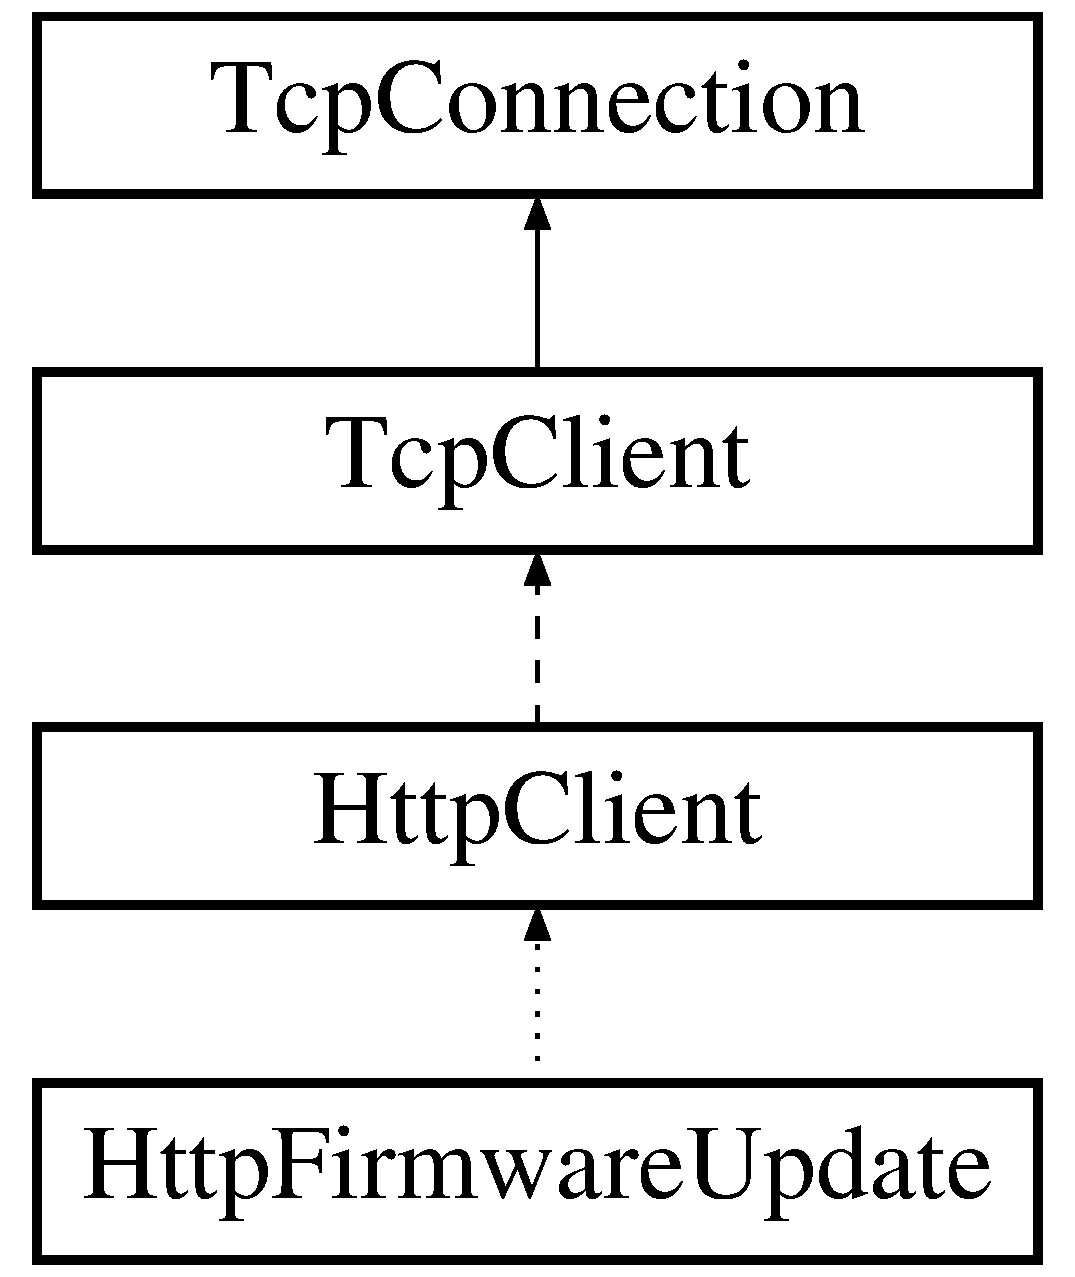
\includegraphics[height=4.000000cm]{class_http_client}
\end{center}
\end{figure}
\subsection*{Public Member Functions}
\begin{DoxyCompactItemize}
\item 
\hypertarget{class_http_client_a1283ada5645c88489bb04b8967d95f38}{}{\bfseries Http\+Client} (bool auto\+Destruct=false)\label{class_http_client_a1283ada5645c88489bb04b8967d95f38}

\item 
\hypertarget{class_http_client_acff314267ac228a0fda846164cc9b35c}{}bool {\bfseries download\+String} (String url, \hyperlink{class_delegate}{Http\+Client\+Completed\+Callback} on\+Completed)\label{class_http_client_acff314267ac228a0fda846164cc9b35c}

\item 
\hypertarget{class_http_client_ad2ea502457a5b753ee5cbe9a65ee9d2c}{}String {\bfseries get\+Response\+String} ()\label{class_http_client_ad2ea502457a5b753ee5cbe9a65ee9d2c}

\item 
\hypertarget{class_http_client_a416faa1d1a175d8e3662a5cf48e7069c}{}bool {\bfseries download\+File} (String url, \hyperlink{class_delegate}{Http\+Client\+Completed\+Callback} on\+Completed=N\+U\+L\+L)\label{class_http_client_a416faa1d1a175d8e3662a5cf48e7069c}

\item 
\hypertarget{class_http_client_a5bc8fe1f56d493658f0535752256cc46}{}bool {\bfseries download\+File} (String url, String save\+File\+Name, \hyperlink{class_delegate}{Http\+Client\+Completed\+Callback} on\+Completed=N\+U\+L\+L)\label{class_http_client_a5bc8fe1f56d493658f0535752256cc46}

\item 
\hypertarget{class_http_client_ab423ad5713fb9f2569443c18c4b51d9a}{}void {\bfseries set\+Post\+Body} (String \+\_\+method)\label{class_http_client_ab423ad5713fb9f2569443c18c4b51d9a}

\item 
\hypertarget{class_http_client_a79395f514b78c5f0366571ed613a3151}{}String {\bfseries get\+Post\+Body} ()\label{class_http_client_a79395f514b78c5f0366571ed613a3151}

\item 
\hypertarget{class_http_client_a8faf4657baf0255f1b504fe771708acb}{}void {\bfseries set\+Content\+Type} (String \+\_\+content\+\_\+type)\label{class_http_client_a8faf4657baf0255f1b504fe771708acb}

\item 
\hypertarget{class_http_client_ac22516dfd9d8ac4db332cd25000528ef}{}String {\bfseries get\+Content\+Type} ()\label{class_http_client_ac22516dfd9d8ac4db332cd25000528ef}

\item 
\hypertarget{class_http_client_a0eeebce9727415d6a7fce58e5512a74b}{}\+\_\+\+\_\+forceinline int {\bfseries get\+Reponse\+Code} ()\label{class_http_client_a0eeebce9727415d6a7fce58e5512a74b}

\item 
\hypertarget{class_http_client_a06a7fec48b726f4351606267d4afceb9}{}\+\_\+\+\_\+forceinline bool {\bfseries is\+Successful} ()\label{class_http_client_a06a7fec48b726f4351606267d4afceb9}

\item 
\hypertarget{class_http_client_a56fdb130ddfb0a6e6c17d6110d644345}{}\+\_\+\+\_\+forceinline bool {\bfseries is\+Processing} ()\label{class_http_client_a56fdb130ddfb0a6e6c17d6110d644345}

\item 
\hypertarget{class_http_client_a3967c52ec17e82f469e6d96c00210e7a}{}\+\_\+\+\_\+forceinline Tcp\+Client\+State {\bfseries get\+State} ()\label{class_http_client_a3967c52ec17e82f469e6d96c00210e7a}

\item 
\hypertarget{class_http_client_acb02f4ea408d30405d0f7786810f4db0}{}String {\bfseries get\+Response\+Header} (String header\+Name, String default\+Value=\char`\"{}\char`\"{})\label{class_http_client_acb02f4ea408d30405d0f7786810f4db0}

\item 
\hypertarget{class_http_client_a486812ccc76aa2f9d5bae27b2e46f4dc}{}\hyperlink{class_date_time}{Date\+Time} {\bfseries get\+Last\+Modified\+Date} ()\label{class_http_client_a486812ccc76aa2f9d5bae27b2e46f4dc}

\item 
\hypertarget{class_http_client_af56610a0d5b1e5f36b56ffab0f3d0134}{}\hyperlink{class_date_time}{Date\+Time} {\bfseries get\+Server\+Date} ()\label{class_http_client_af56610a0d5b1e5f36b56ffab0f3d0134}

\item 
\hypertarget{class_http_client_add736676d2310312697766b3fa1cc54d}{}void {\bfseries reset} ()\label{class_http_client_add736676d2310312697766b3fa1cc54d}

\end{DoxyCompactItemize}
\subsection*{Protected Member Functions}
\begin{DoxyCompactItemize}
\item 
\hypertarget{class_http_client_a448c7837bda53245ff1485e4e7db6827}{}bool {\bfseries start\+Download} (\hyperlink{class_u_r_l}{U\+R\+L} uri, Http\+Client\+Mode mode, \hyperlink{class_delegate}{Http\+Client\+Completed\+Callback} on\+Completed)\label{class_http_client_a448c7837bda53245ff1485e4e7db6827}

\item 
\hypertarget{class_http_client_a01b19eb339cb8a903a3c244aec115f06}{}void {\bfseries on\+Finished} (Tcp\+Client\+State finish\+State)\label{class_http_client_a01b19eb339cb8a903a3c244aec115f06}

\item 
\hypertarget{class_http_client_a5ea5de376338b972c616f00a669f7117}{}virtual err\+\_\+t {\bfseries on\+Receive} (\hyperlink{structpbuf}{pbuf} $\ast$buf)\label{class_http_client_a5ea5de376338b972c616f00a669f7117}

\item 
\hypertarget{class_http_client_a5d6e23d4703e6439787393399e0fb82c}{}virtual void {\bfseries write\+Raw\+Data} (\hyperlink{structpbuf}{pbuf} $\ast$buf, int start\+Pos)\label{class_http_client_a5d6e23d4703e6439787393399e0fb82c}

\item 
\hypertarget{class_http_client_a561c94d8a5ca8e662a20912747ae07da}{}void {\bfseries parse\+Headers} (\hyperlink{structpbuf}{pbuf} $\ast$buf, int header\+End)\label{class_http_client_a561c94d8a5ca8e662a20912747ae07da}

\end{DoxyCompactItemize}
\subsection*{Protected Attributes}
\begin{DoxyCompactItemize}
\item 
\hypertarget{class_http_client_a95b753e9c9b75aedf4f8635c7400be77}{}bool {\bfseries wait\+Parse}\label{class_http_client_a95b753e9c9b75aedf4f8635c7400be77}

\item 
\hypertarget{class_http_client_a7274432e4a75417628d8bb236f3da2e5}{}bool {\bfseries write\+Error}\label{class_http_client_a7274432e4a75417628d8bb236f3da2e5}

\end{DoxyCompactItemize}
\subsection*{Additional Inherited Members}


The documentation for this class was generated from the following files\+:\begin{DoxyCompactItemize}
\item 
Sming\+Core/\+Network/Http\+Client.\+h\item 
Sming\+Core/\+Network/Http\+Client.\+cpp\end{DoxyCompactItemize}

\hypertarget{class_http_firmware_update}{}\section{Http\+Firmware\+Update Class Reference}
\label{class_http_firmware_update}\index{Http\+Firmware\+Update@{Http\+Firmware\+Update}}
Inheritance diagram for Http\+Firmware\+Update\+:\begin{figure}[H]
\begin{center}
\leavevmode
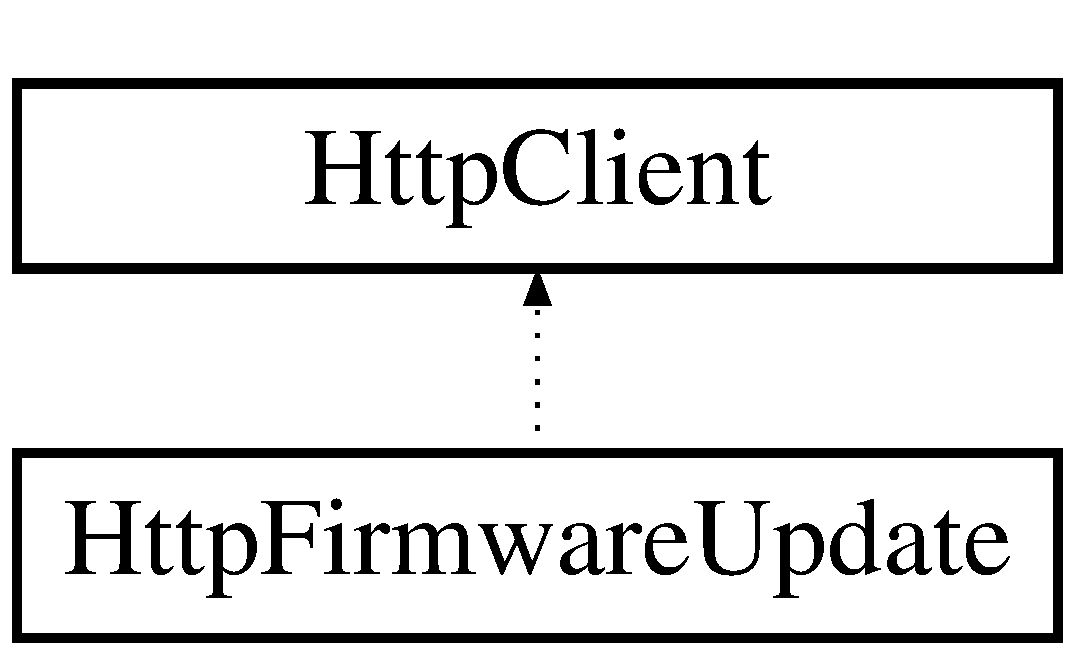
\includegraphics[height=2.000000cm]{class_http_firmware_update}
\end{center}
\end{figure}
\subsection*{Public Member Functions}
\begin{DoxyCompactItemize}
\item 
\hypertarget{class_http_firmware_update_a9308f2da7166cf51d62c01fddd9d3d1a}{}void {\bfseries add\+Item} (int offset, String firmware\+File\+Url)\label{class_http_firmware_update_a9308f2da7166cf51d62c01fddd9d3d1a}

\item 
\hypertarget{class_http_firmware_update_a9e8cdf39684e797beda0508e87276d6d}{}void {\bfseries start} ()\label{class_http_firmware_update_a9e8cdf39684e797beda0508e87276d6d}

\end{DoxyCompactItemize}
\subsection*{Protected Member Functions}
\begin{DoxyCompactItemize}
\item 
\hypertarget{class_http_firmware_update_a1991f3eabc3b4b8d639a77aab749d653}{}void {\bfseries on\+Timer} ()\label{class_http_firmware_update_a1991f3eabc3b4b8d639a77aab749d653}

\item 
\hypertarget{class_http_firmware_update_af13d1432dbd2e89707ae5e740572f1f2}{}virtual void {\bfseries write\+Raw\+Data} (\hyperlink{structpbuf}{pbuf} $\ast$buf, int start\+Pos)\label{class_http_firmware_update_af13d1432dbd2e89707ae5e740572f1f2}

\item 
\hypertarget{class_http_firmware_update_a4f5e354f43f85f57064d262bff108520}{}uint32\+\_\+t {\bfseries write\+Flash} (char $\ast$data, uint32\+\_\+t pos, int size)\label{class_http_firmware_update_a4f5e354f43f85f57064d262bff108520}

\item 
\hypertarget{class_http_firmware_update_aab35ec18c670859bffedc49b53a63afb}{}void {\bfseries apply\+Update} ()\label{class_http_firmware_update_aab35ec18c670859bffedc49b53a63afb}

\end{DoxyCompactItemize}
\subsection*{Static Protected Member Functions}
\begin{DoxyCompactItemize}
\item 
\hypertarget{class_http_firmware_update_a2a17245cbc6850ef011967120b62dc26}{}static void {\bfseries static\+On\+Timer} (void $\ast$ptr\+Self)\label{class_http_firmware_update_a2a17245cbc6850ef011967120b62dc26}

\end{DoxyCompactItemize}
\subsection*{Protected Attributes}
\begin{DoxyCompactItemize}
\item 
\hypertarget{class_http_firmware_update_ae38c2e3ff45204385b84b7bb94790099}{}\hyperlink{class_vector}{Vector}$<$ \hyperlink{struct_http_firmware_update_item}{Http\+Firmware\+Update\+Item} $>$ {\bfseries items}\label{class_http_firmware_update_ae38c2e3ff45204385b84b7bb94790099}

\item 
\hypertarget{class_http_firmware_update_a9c1cf4d965bcab54c7519c8bb06b632b}{}E\+T\+S\+Timer {\bfseries timer}\label{class_http_firmware_update_a9c1cf4d965bcab54c7519c8bb06b632b}

\item 
\hypertarget{class_http_firmware_update_a5272fba1a38647606d8b93da3aec1e61}{}int {\bfseries current\+Item}\label{class_http_firmware_update_a5272fba1a38647606d8b93da3aec1e61}

\item 
\hypertarget{class_http_firmware_update_a5dd41a15dfc83b707e087c5c528cf99e}{}uint32\+\_\+t {\bfseries pos}\label{class_http_firmware_update_a5dd41a15dfc83b707e087c5c528cf99e}

\end{DoxyCompactItemize}


The documentation for this class was generated from the following files\+:\begin{DoxyCompactItemize}
\item 
Sming\+Core/\+Network/Http\+Firmware\+Update.\+h\item 
Sming\+Core/\+Network/Http\+Firmware\+Update.\+cpp\end{DoxyCompactItemize}

\hypertarget{struct_http_firmware_update_item}{}\section{Http\+Firmware\+Update\+Item Struct Reference}
\label{struct_http_firmware_update_item}\index{Http\+Firmware\+Update\+Item@{Http\+Firmware\+Update\+Item}}
\subsection*{Public Attributes}
\begin{DoxyCompactItemize}
\item 
\hypertarget{struct_http_firmware_update_item_a0d5a9f9ff25c356685303c1f79634840}{}String {\bfseries url}\label{struct_http_firmware_update_item_a0d5a9f9ff25c356685303c1f79634840}

\item 
\hypertarget{struct_http_firmware_update_item_a0f5c54f7221fbfbebe94a67b659e166a}{}uint32\+\_\+t {\bfseries target\+Offset}\label{struct_http_firmware_update_item_a0f5c54f7221fbfbebe94a67b659e166a}

\item 
\hypertarget{struct_http_firmware_update_item_aaf6051dbec373d4bfe116b7d25497f74}{}uint32\+\_\+t {\bfseries flash}\label{struct_http_firmware_update_item_aaf6051dbec373d4bfe116b7d25497f74}

\item 
\hypertarget{struct_http_firmware_update_item_af546c18fb8e76c1c11e283b78527bed2}{}int {\bfseries size}\label{struct_http_firmware_update_item_af546c18fb8e76c1c11e283b78527bed2}

\end{DoxyCompactItemize}


The documentation for this struct was generated from the following file\+:\begin{DoxyCompactItemize}
\item 
Sming\+Core/\+Network/Http\+Firmware\+Update.\+h\end{DoxyCompactItemize}

\hypertarget{class_http_request}{}\section{Http\+Request Class Reference}
\label{class_http_request}\index{Http\+Request@{Http\+Request}}
\subsection*{Public Member Functions}
\begin{DoxyCompactItemize}
\item 
\hypertarget{class_http_request_a286a1331701444b0c4ab04858a282c18}{}String {\bfseries get\+Request\+Method} ()\label{class_http_request_a286a1331701444b0c4ab04858a282c18}

\item 
\hypertarget{class_http_request_aac3961439d9ed0645b8acd753b8207ec}{}String {\bfseries get\+Path} ()\label{class_http_request_aac3961439d9ed0645b8acd753b8207ec}

\item 
\hypertarget{class_http_request_a72f9f4efa9ab95444ca5391dd144eec3}{}String {\bfseries get\+Content\+Type} ()\label{class_http_request_a72f9f4efa9ab95444ca5391dd144eec3}

\item 
\hypertarget{class_http_request_ad61cfcb6b2de741f0cf61473cf5ac1c4}{}int {\bfseries get\+Content\+Length} ()\label{class_http_request_ad61cfcb6b2de741f0cf61473cf5ac1c4}

\item 
\hypertarget{class_http_request_a200ace2d6dead0e314f80a55385b3378}{}String {\bfseries get\+Query\+Parameter} (String parameter\+Name, String default\+Value=\char`\"{}\char`\"{})\label{class_http_request_a200ace2d6dead0e314f80a55385b3378}

\item 
\hypertarget{class_http_request_a4d150360974338f51a8577ac0db4d8c0}{}String {\bfseries get\+Post\+Parameter} (String parameter\+Name, String default\+Value=\char`\"{}\char`\"{})\label{class_http_request_a4d150360974338f51a8577ac0db4d8c0}

\item 
\hypertarget{class_http_request_a9a47518aeb930576b337be2dc7926aab}{}String {\bfseries get\+Header} (String header\+Name, String default\+Value=\char`\"{}\char`\"{})\label{class_http_request_a9a47518aeb930576b337be2dc7926aab}

\item 
\hypertarget{class_http_request_aa138554e168a1fc98a43c0fb99403b26}{}String {\bfseries get\+Cookie} (String cookie\+Name, String default\+Value=\char`\"{}\char`\"{})\label{class_http_request_aa138554e168a1fc98a43c0fb99403b26}

\item 
\hypertarget{class_http_request_a9dfe3aabfd7e8c48006e76d7f37d1d83}{}Http\+Parse\+Result {\bfseries parse\+Header} (\hyperlink{class_http_server}{Http\+Server} $\ast$server, \hyperlink{structpbuf}{pbuf} $\ast$buf)\label{class_http_request_a9dfe3aabfd7e8c48006e76d7f37d1d83}

\item 
\hypertarget{class_http_request_acb0876ae302749797b914165d79b30d7}{}Http\+Parse\+Result {\bfseries parse\+Post\+Data} (\hyperlink{class_http_server}{Http\+Server} $\ast$server, \hyperlink{structpbuf}{pbuf} $\ast$buf)\label{class_http_request_acb0876ae302749797b914165d79b30d7}

\item 
\hypertarget{class_http_request_a6be563a3491ca7fcec555c04c94021d6}{}bool {\bfseries extract\+Parsing\+Items\+List} (\hyperlink{structpbuf}{pbuf} $\ast$buf, int start\+Pos, int end\+Pos, char delim\+Char, char end\+Char, \hyperlink{class_hash_map}{Hash\+Map}$<$ String, String $>$ $\ast$result\+Items)\label{class_http_request_a6be563a3491ca7fcec555c04c94021d6}

\end{DoxyCompactItemize}
\subsection*{Friends}
\begin{DoxyCompactItemize}
\item 
\hypertarget{class_http_request_a329df4515861a7be30b085849c292914}{}class {\bfseries Template\+File\+Stream}\label{class_http_request_a329df4515861a7be30b085849c292914}

\end{DoxyCompactItemize}


The documentation for this class was generated from the following files\+:\begin{DoxyCompactItemize}
\item 
Sming\+Core/\+Network/Http\+Request.\+h\item 
Sming\+Core/\+Network/Http\+Request.\+cpp\end{DoxyCompactItemize}

\hypertarget{class_http_response}{}\section{Http\+Response Class Reference}
\label{class_http_response}\index{Http\+Response@{Http\+Response}}
\subsection*{Public Member Functions}
\begin{DoxyCompactItemize}
\item 
\hypertarget{class_http_response_a6ddc1855eb97864ffef28eb9a491358b}{}void {\bfseries bad\+Request} ()\label{class_http_response_a6ddc1855eb97864ffef28eb9a491358b}

\item 
\hypertarget{class_http_response_ab710c73aa65ac0506d130f6841e6194a}{}void {\bfseries not\+Found} ()\label{class_http_response_ab710c73aa65ac0506d130f6841e6194a}

\item 
\hypertarget{class_http_response_a1e5c9dd005e4e7afd1f99308b5460b2d}{}void {\bfseries forbidden} ()\label{class_http_response_a1e5c9dd005e4e7afd1f99308b5460b2d}

\item 
\hypertarget{class_http_response_aa91856817a881e9bd6db0b837e68b2c0}{}void {\bfseries authorization\+Required} ()\label{class_http_response_aa91856817a881e9bd6db0b837e68b2c0}

\item 
\hypertarget{class_http_response_abbe53a6919902bfb8b254fab864ae175}{}void {\bfseries redirect} (String location=\char`\"{}\char`\"{})\label{class_http_response_abbe53a6919902bfb8b254fab864ae175}

\item 
\hypertarget{class_http_response_ae1f5df51a03dfbcad9d82d650418713a}{}void {\bfseries set\+Content\+Type} (const String type)\label{class_http_response_ae1f5df51a03dfbcad9d82d650418713a}

\item 
\hypertarget{class_http_response_af91b228bc40b7222557b24d1d97601ad}{}void {\bfseries set\+Cookie} (const String name, const String value)\label{class_http_response_af91b228bc40b7222557b24d1d97601ad}

\item 
\hypertarget{class_http_response_a2e556aaccd751726df7ee1dc8dc95dca}{}void {\bfseries set\+Header} (const String name, const String value)\label{class_http_response_a2e556aaccd751726df7ee1dc8dc95dca}

\item 
\hypertarget{class_http_response_af7ca427335e5e6c6472ae031a8787d70}{}bool {\bfseries has\+Header} (const String name)\label{class_http_response_af7ca427335e5e6c6472ae031a8787d70}

\item 
\hypertarget{class_http_response_a097289521073c2f83c0c3edbee0eec23}{}void {\bfseries set\+Cache} (int max\+Age\+Seconds=3600, bool is\+Public=false)\label{class_http_response_a097289521073c2f83c0c3edbee0eec23}

\item 
\hypertarget{class_http_response_acd6c13889d13cf411e7e3ab34354664d}{}void {\bfseries set\+Allow\+Cross\+Domain\+Origin} (String control\+Allow\+Origin)\label{class_http_response_acd6c13889d13cf411e7e3ab34354664d}

\item 
\hypertarget{class_http_response_a376d0bd8b7fbf9facb99134583ae2ed1}{}String {\bfseries get\+Status\+Name} ()\label{class_http_response_a376d0bd8b7fbf9facb99134583ae2ed1}

\item 
\hypertarget{class_http_response_a6906d59ec9169d518e2bf9abada484ae}{}int {\bfseries get\+Status\+Code} ()\label{class_http_response_a6906d59ec9169d518e2bf9abada484ae}

\item 
\hypertarget{class_http_response_ae8045d121a30f6d7d0e21aa6cc412b97}{}bool {\bfseries has\+Body} ()\label{class_http_response_ae8045d121a30f6d7d0e21aa6cc412b97}

\item 
\hypertarget{class_http_response_aafed32c182626bb9f384105b2741d6b1}{}void {\bfseries send\+String} (const char $\ast$string)\label{class_http_response_aafed32c182626bb9f384105b2741d6b1}

\item 
\hypertarget{class_http_response_afb7fa4e217cfa24ee5afa00b63da761e}{}void {\bfseries send\+String} (String string)\label{class_http_response_afb7fa4e217cfa24ee5afa00b63da761e}

\item 
\hypertarget{class_http_response_a5ac8fc1d595d26d0e43b7429ac640743}{}bool {\bfseries send\+File} (String file\+Name, bool allow\+Gzip\+File\+Check=true)\label{class_http_response_a5ac8fc1d595d26d0e43b7429ac640743}

\item 
\hypertarget{class_http_response_a8e389f1caa47c5d77a9d0dd14ea15905}{}bool {\bfseries send\+Template} (\hyperlink{class_template_file_stream}{Template\+File\+Stream} $\ast$new\+Template\+Instance)\label{class_http_response_a8e389f1caa47c5d77a9d0dd14ea15905}

\item 
\hypertarget{class_http_response_a4ad42c6da411ab80d938f1f07e77171d}{}bool {\bfseries send\+Json\+Object} (\hyperlink{class_json_object_stream}{Json\+Object\+Stream} $\ast$new\+Json\+Stream\+Instance)\label{class_http_response_a4ad42c6da411ab80d938f1f07e77171d}

\item 
\hypertarget{class_http_response_a522560820fec07c4f1f8675699d85887}{}void {\bfseries send\+Header} (\hyperlink{class_http_server_connection}{Http\+Server\+Connection} \&connection)\label{class_http_response_a522560820fec07c4f1f8675699d85887}

\item 
\hypertarget{class_http_response_a57b20ddbf914fb287f4c321b93a872fe}{}bool {\bfseries send\+Body} (\hyperlink{class_http_server_connection}{Http\+Server\+Connection} \&connection)\label{class_http_response_a57b20ddbf914fb287f4c321b93a872fe}

\end{DoxyCompactItemize}


The documentation for this class was generated from the following files\+:\begin{DoxyCompactItemize}
\item 
Sming\+Core/\+Network/Http\+Response.\+h\item 
Sming\+Core/\+Network/Http\+Response.\+cpp\end{DoxyCompactItemize}

\hypertarget{class_http_server}{}\section{Http\+Server Class Reference}
\label{class_http_server}\index{Http\+Server@{Http\+Server}}
Inheritance diagram for Http\+Server\+:\begin{figure}[H]
\begin{center}
\leavevmode
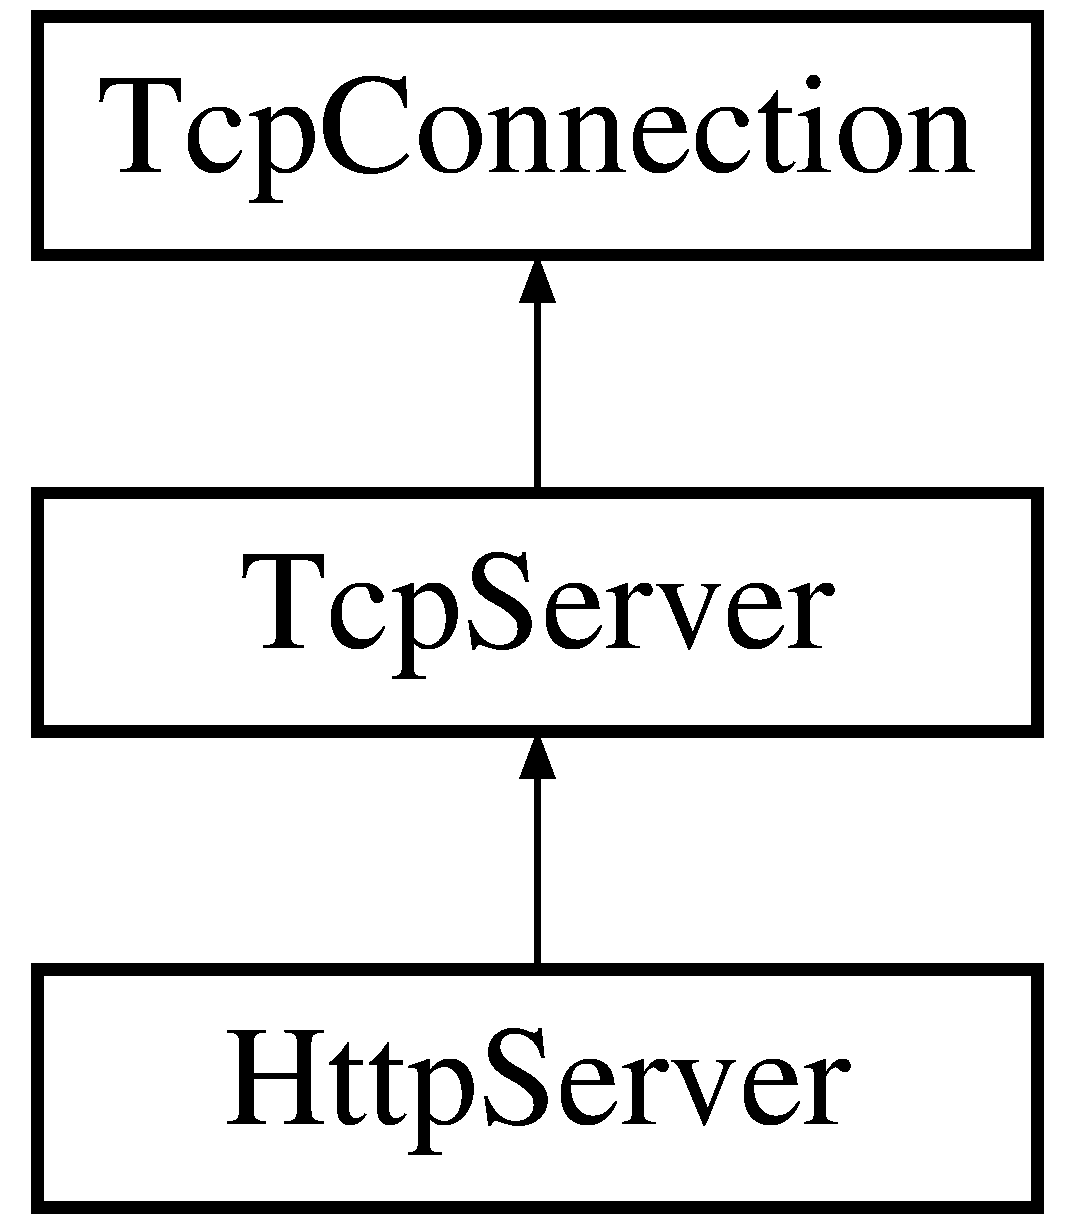
\includegraphics[height=3.000000cm]{class_http_server}
\end{center}
\end{figure}
\subsection*{Public Member Functions}
\begin{DoxyCompactItemize}
\item 
\hypertarget{class_http_server_aff1d6aa5491cb05d48162ee36c053f7e}{}void {\bfseries enable\+Header\+Processing} (String header\+Name)\label{class_http_server_aff1d6aa5491cb05d48162ee36c053f7e}

\item 
\hypertarget{class_http_server_aec0af0131fb2b96868759cd5901813da}{}bool {\bfseries is\+Header\+Processing\+Enabled} (String name)\label{class_http_server_aec0af0131fb2b96868759cd5901813da}

\item 
\hypertarget{class_http_server_ad0bd05da46ae1bec9a4e3bc824f43ad1}{}void {\bfseries add\+Path} (String path, \hyperlink{class_delegate}{Http\+Path\+Callback} callback)\label{class_http_server_ad0bd05da46ae1bec9a4e3bc824f43ad1}

\item 
\hypertarget{class_http_server_afa5843b00c8021851105e3cc5ced17eb}{}void {\bfseries set\+Default\+Handler} (\hyperlink{class_delegate}{Http\+Path\+Callback} callback)\label{class_http_server_afa5843b00c8021851105e3cc5ced17eb}

\item 
\hypertarget{class_http_server_ab552d521b9e702c26aab4c3df9ca5bc5}{}bool {\bfseries process} (\hyperlink{class_http_server_connection}{Http\+Server\+Connection} \&connection, \hyperlink{class_http_request}{Http\+Request} \&request, \hyperlink{class_http_response}{Http\+Response} \&response)\label{class_http_server_ab552d521b9e702c26aab4c3df9ca5bc5}

\end{DoxyCompactItemize}
\subsection*{Protected Member Functions}
\begin{DoxyCompactItemize}
\item 
\hypertarget{class_http_server_a4f1d6dea4a489d13b9ef6e690090acb6}{}virtual \hyperlink{class_tcp_connection}{Tcp\+Connection} $\ast$ {\bfseries create\+Client} (tcp\+\_\+pcb $\ast$client\+Tcp)\label{class_http_server_a4f1d6dea4a489d13b9ef6e690090acb6}

\end{DoxyCompactItemize}
\subsection*{Additional Inherited Members}


The documentation for this class was generated from the following files\+:\begin{DoxyCompactItemize}
\item 
Sming\+Core/\+Network/Http\+Server.\+h\item 
Sming\+Core/\+Network/Http\+Server.\+cpp\end{DoxyCompactItemize}

\hypertarget{class_http_server_connection}{}\section{Http\+Server\+Connection Class Reference}
\label{class_http_server_connection}\index{Http\+Server\+Connection@{Http\+Server\+Connection}}
Inheritance diagram for Http\+Server\+Connection\+:\begin{figure}[H]
\begin{center}
\leavevmode
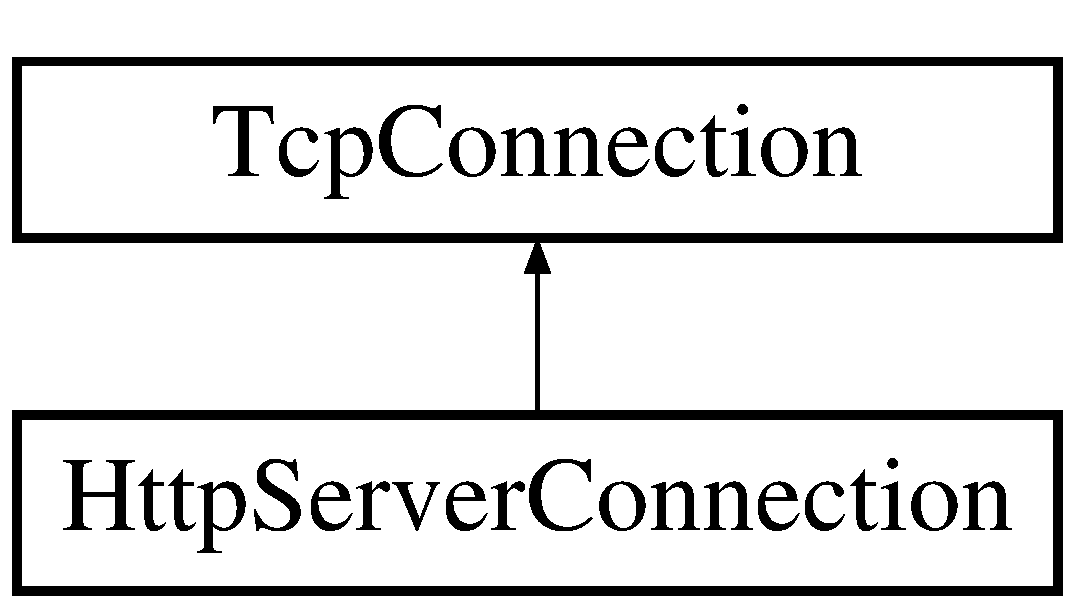
\includegraphics[height=2.000000cm]{class_http_server_connection}
\end{center}
\end{figure}
\subsection*{Public Member Functions}
\begin{DoxyCompactItemize}
\item 
\hypertarget{class_http_server_connection_a932d7972bfb9cc55785bca493a64fc81}{}{\bfseries Http\+Server\+Connection} (\hyperlink{class_http_server}{Http\+Server} $\ast$parent\+Server, tcp\+\_\+pcb $\ast$client\+Tcp)\label{class_http_server_connection_a932d7972bfb9cc55785bca493a64fc81}

\end{DoxyCompactItemize}
\subsection*{Protected Member Functions}
\begin{DoxyCompactItemize}
\item 
\hypertarget{class_http_server_connection_ae758702ac20ec7bbd48955fe58619580}{}virtual err\+\_\+t {\bfseries on\+Receive} (\hyperlink{structpbuf}{pbuf} $\ast$buf)\label{class_http_server_connection_ae758702ac20ec7bbd48955fe58619580}

\item 
\hypertarget{class_http_server_connection_afba7fcad9ff3ed848eaba6a807c35cdd}{}virtual void {\bfseries on\+Ready\+To\+Send\+Data} (Tcp\+Connection\+Event source\+Event)\label{class_http_server_connection_afba7fcad9ff3ed848eaba6a807c35cdd}

\item 
\hypertarget{class_http_server_connection_a5e3e907b120513dac55004bafa61a39b}{}virtual void {\bfseries begin\+Send\+Data} ()\label{class_http_server_connection_a5e3e907b120513dac55004bafa61a39b}

\item 
\hypertarget{class_http_server_connection_acbd41eed522aca1b478cb723ef02736b}{}virtual void {\bfseries send\+Error} (const char $\ast$message=N\+U\+L\+L)\label{class_http_server_connection_acbd41eed522aca1b478cb723ef02736b}

\end{DoxyCompactItemize}
\subsection*{Friends}
\begin{DoxyCompactItemize}
\item 
\hypertarget{class_http_server_connection_a48233feea8fcb70b62dd61a3bb860c9d}{}class {\bfseries Http\+Response}\label{class_http_server_connection_a48233feea8fcb70b62dd61a3bb860c9d}

\item 
\hypertarget{class_http_server_connection_a3158ef04d4a1177eb6a5e64d87a6801c}{}class {\bfseries Http\+Request}\label{class_http_server_connection_a3158ef04d4a1177eb6a5e64d87a6801c}

\end{DoxyCompactItemize}
\subsection*{Additional Inherited Members}


The documentation for this class was generated from the following files\+:\begin{DoxyCompactItemize}
\item 
Sming\+Core/\+Network/Http\+Server\+Connection.\+h\item 
Sming\+Core/\+Network/Http\+Server\+Connection.\+cpp\end{DoxyCompactItemize}

\hypertarget{class_i2_cdev}{}\section{I2\+Cdev Class Reference}
\label{class_i2_cdev}\index{I2\+Cdev@{I2\+Cdev}}
\subsection*{Public Member Functions}
\begin{DoxyCompactItemize}
\item 
\hyperlink{class_i2_cdev_a0a466e2323d9f719a1ecc9fa11ac5c84}{I2\+Cdev} ()
\end{DoxyCompactItemize}
\subsection*{Static Public Member Functions}
\begin{DoxyCompactItemize}
\item 
static int8\+\_\+t \hyperlink{class_i2_cdev_abe6d8ea07027d362419de86188981559}{read\+Bit} (uint8\+\_\+t dev\+Addr, uint8\+\_\+t reg\+Addr, uint8\+\_\+t bit\+Num, uint8\+\_\+t $\ast$data, uint16\+\_\+t timeout=\hyperlink{class_i2_cdev_ae2125796e0948127fc15031650111e82}{I2\+Cdev\+::read\+Timeout})
\item 
static int8\+\_\+t \hyperlink{class_i2_cdev_aaaa3b9ef9500a7d69ccc3d0ccaae33c4}{read\+Bit\+W} (uint8\+\_\+t dev\+Addr, uint8\+\_\+t reg\+Addr, uint8\+\_\+t bit\+Num, uint16\+\_\+t $\ast$data, uint16\+\_\+t timeout=\hyperlink{class_i2_cdev_ae2125796e0948127fc15031650111e82}{I2\+Cdev\+::read\+Timeout})
\item 
static int8\+\_\+t \hyperlink{class_i2_cdev_a8e5e9742072bb80db06ccd46f52e2b6d}{read\+Bits} (uint8\+\_\+t dev\+Addr, uint8\+\_\+t reg\+Addr, uint8\+\_\+t bit\+Start, uint8\+\_\+t length, uint8\+\_\+t $\ast$data, uint16\+\_\+t timeout=\hyperlink{class_i2_cdev_ae2125796e0948127fc15031650111e82}{I2\+Cdev\+::read\+Timeout})
\item 
static int8\+\_\+t \hyperlink{class_i2_cdev_a1f417ba3e5ce99832e07c31522c97f87}{read\+Bits\+W} (uint8\+\_\+t dev\+Addr, uint8\+\_\+t reg\+Addr, uint8\+\_\+t bit\+Start, uint8\+\_\+t length, uint16\+\_\+t $\ast$data, uint16\+\_\+t timeout=\hyperlink{class_i2_cdev_ae2125796e0948127fc15031650111e82}{I2\+Cdev\+::read\+Timeout})
\item 
static int8\+\_\+t \hyperlink{class_i2_cdev_ad3fb41ce124a29f93749d99611c75c33}{read\+Byte} (uint8\+\_\+t dev\+Addr, uint8\+\_\+t reg\+Addr, uint8\+\_\+t $\ast$data, uint16\+\_\+t timeout=\hyperlink{class_i2_cdev_ae2125796e0948127fc15031650111e82}{I2\+Cdev\+::read\+Timeout})
\item 
static int8\+\_\+t \hyperlink{class_i2_cdev_a545cd48b1e806e7e467b542c9e38e8c8}{read\+Word} (uint8\+\_\+t dev\+Addr, uint8\+\_\+t reg\+Addr, uint16\+\_\+t $\ast$data, uint16\+\_\+t timeout=\hyperlink{class_i2_cdev_ae2125796e0948127fc15031650111e82}{I2\+Cdev\+::read\+Timeout})
\item 
static int8\+\_\+t \hyperlink{class_i2_cdev_aca9c503da5cffd6ac6f8eff9b195c5f4}{read\+Bytes} (uint8\+\_\+t dev\+Addr, uint8\+\_\+t reg\+Addr, uint8\+\_\+t length, uint8\+\_\+t $\ast$data, uint16\+\_\+t timeout=\hyperlink{class_i2_cdev_ae2125796e0948127fc15031650111e82}{I2\+Cdev\+::read\+Timeout})
\item 
static int8\+\_\+t \hyperlink{class_i2_cdev_a1b3d895dc6a00cbb5fb3b0441b2e35de}{read\+Words} (uint8\+\_\+t dev\+Addr, uint8\+\_\+t reg\+Addr, uint8\+\_\+t length, uint16\+\_\+t $\ast$data, uint16\+\_\+t timeout=\hyperlink{class_i2_cdev_ae2125796e0948127fc15031650111e82}{I2\+Cdev\+::read\+Timeout})
\item 
static bool \hyperlink{class_i2_cdev_aa68890af87de5471d32e583ebbd91acb}{write\+Bit} (uint8\+\_\+t dev\+Addr, uint8\+\_\+t reg\+Addr, uint8\+\_\+t bit\+Num, uint8\+\_\+t data)
\item 
static bool \hyperlink{class_i2_cdev_a1b5fbedfadec5d429c81ee84d27e658d}{write\+Bit\+W} (uint8\+\_\+t dev\+Addr, uint8\+\_\+t reg\+Addr, uint8\+\_\+t bit\+Num, uint16\+\_\+t data)
\item 
static bool \hyperlink{class_i2_cdev_a913371251b6a41520c080115650e1b59}{write\+Bits} (uint8\+\_\+t dev\+Addr, uint8\+\_\+t reg\+Addr, uint8\+\_\+t bit\+Start, uint8\+\_\+t length, uint8\+\_\+t data)
\item 
static bool \hyperlink{class_i2_cdev_a8f8652a1328224cce867eed665a45c4d}{write\+Bits\+W} (uint8\+\_\+t dev\+Addr, uint8\+\_\+t reg\+Addr, uint8\+\_\+t bit\+Start, uint8\+\_\+t length, uint16\+\_\+t data)
\item 
static bool \hyperlink{class_i2_cdev_aeb297637ef985cd562da465ba61b7042}{write\+Byte} (uint8\+\_\+t dev\+Addr, uint8\+\_\+t reg\+Addr, uint8\+\_\+t data)
\item 
static bool \hyperlink{class_i2_cdev_acbe68a802d6a177301736e60bedd1def}{write\+Word} (uint8\+\_\+t dev\+Addr, uint8\+\_\+t reg\+Addr, uint16\+\_\+t data)
\item 
static bool \hyperlink{class_i2_cdev_aa4e39cac6c0eac5112f9132084bcc93e}{write\+Bytes} (uint8\+\_\+t dev\+Addr, uint8\+\_\+t reg\+Addr, uint8\+\_\+t length, uint8\+\_\+t $\ast$data)
\item 
static bool \hyperlink{class_i2_cdev_aae37c0526e4b4730a5b2ffd752fd8b21}{write\+Words} (uint8\+\_\+t dev\+Addr, uint8\+\_\+t reg\+Addr, uint8\+\_\+t length, uint16\+\_\+t $\ast$data)
\end{DoxyCompactItemize}
\subsection*{Static Public Attributes}
\begin{DoxyCompactItemize}
\item 
static uint16\+\_\+t \hyperlink{class_i2_cdev_ae2125796e0948127fc15031650111e82}{read\+Timeout} = I2\+C\+D\+E\+V\+\_\+\+D\+E\+F\+A\+U\+L\+T\+\_\+\+R\+E\+A\+D\+\_\+\+T\+I\+M\+E\+O\+U\+T
\end{DoxyCompactItemize}


\subsection{Constructor \& Destructor Documentation}
\hypertarget{class_i2_cdev_a0a466e2323d9f719a1ecc9fa11ac5c84}{}\index{I2\+Cdev@{I2\+Cdev}!I2\+Cdev@{I2\+Cdev}}
\index{I2\+Cdev@{I2\+Cdev}!I2\+Cdev@{I2\+Cdev}}
\subsubsection[{I2\+Cdev}]{\setlength{\rightskip}{0pt plus 5cm}I2\+Cdev\+::\+I2\+Cdev (
\begin{DoxyParamCaption}
{}
\end{DoxyParamCaption}
)}\label{class_i2_cdev_a0a466e2323d9f719a1ecc9fa11ac5c84}
Default constructor. 

\subsection{Member Function Documentation}
\hypertarget{class_i2_cdev_abe6d8ea07027d362419de86188981559}{}\index{I2\+Cdev@{I2\+Cdev}!read\+Bit@{read\+Bit}}
\index{read\+Bit@{read\+Bit}!I2\+Cdev@{I2\+Cdev}}
\subsubsection[{read\+Bit}]{\setlength{\rightskip}{0pt plus 5cm}int8\+\_\+t I2\+Cdev\+::read\+Bit (
\begin{DoxyParamCaption}
\item[{uint8\+\_\+t}]{dev\+Addr, }
\item[{uint8\+\_\+t}]{reg\+Addr, }
\item[{uint8\+\_\+t}]{bit\+Num, }
\item[{uint8\+\_\+t $\ast$}]{data, }
\item[{uint16\+\_\+t}]{timeout = {\ttfamily {\bf I2\+Cdev\+::read\+Timeout}}}
\end{DoxyParamCaption}
)\hspace{0.3cm}{\ttfamily [static]}}\label{class_i2_cdev_abe6d8ea07027d362419de86188981559}
Read a single bit from an 8-\/bit device register. 
\begin{DoxyParams}{Parameters}
{\em dev\+Addr} & I2\+C slave device address \\
\hline
{\em reg\+Addr} & Register reg\+Addr to read from \\
\hline
{\em bit\+Num} & Bit position to read (0-\/7) \\
\hline
{\em data} & Container for single bit value \\
\hline
{\em timeout} & Optional read timeout in milliseconds (0 to disable, leave off to use default class value in \hyperlink{class_i2_cdev_ae2125796e0948127fc15031650111e82}{I2\+Cdev\+::read\+Timeout}) \\
\hline
\end{DoxyParams}
\begin{DoxyReturn}{Returns}
Status of read operation (true = success) 
\end{DoxyReturn}
\hypertarget{class_i2_cdev_a8e5e9742072bb80db06ccd46f52e2b6d}{}\index{I2\+Cdev@{I2\+Cdev}!read\+Bits@{read\+Bits}}
\index{read\+Bits@{read\+Bits}!I2\+Cdev@{I2\+Cdev}}
\subsubsection[{read\+Bits}]{\setlength{\rightskip}{0pt plus 5cm}int8\+\_\+t I2\+Cdev\+::read\+Bits (
\begin{DoxyParamCaption}
\item[{uint8\+\_\+t}]{dev\+Addr, }
\item[{uint8\+\_\+t}]{reg\+Addr, }
\item[{uint8\+\_\+t}]{bit\+Start, }
\item[{uint8\+\_\+t}]{length, }
\item[{uint8\+\_\+t $\ast$}]{data, }
\item[{uint16\+\_\+t}]{timeout = {\ttfamily {\bf I2\+Cdev\+::read\+Timeout}}}
\end{DoxyParamCaption}
)\hspace{0.3cm}{\ttfamily [static]}}\label{class_i2_cdev_a8e5e9742072bb80db06ccd46f52e2b6d}
Read multiple bits from an 8-\/bit device register. 
\begin{DoxyParams}{Parameters}
{\em dev\+Addr} & I2\+C slave device address \\
\hline
{\em reg\+Addr} & Register reg\+Addr to read from \\
\hline
{\em bit\+Start} & First bit position to read (0-\/7) \\
\hline
{\em length} & Number of bits to read (not more than 8) \\
\hline
{\em data} & Container for right-\/aligned value (i.\+e. \textquotesingle{}101\textquotesingle{} read from any bit\+Start position will equal 0x05) \\
\hline
{\em timeout} & Optional read timeout in milliseconds (0 to disable, leave off to use default class value in \hyperlink{class_i2_cdev_ae2125796e0948127fc15031650111e82}{I2\+Cdev\+::read\+Timeout}) \\
\hline
\end{DoxyParams}
\begin{DoxyReturn}{Returns}
Status of read operation (true = success) 
\end{DoxyReturn}
\hypertarget{class_i2_cdev_a1f417ba3e5ce99832e07c31522c97f87}{}\index{I2\+Cdev@{I2\+Cdev}!read\+Bits\+W@{read\+Bits\+W}}
\index{read\+Bits\+W@{read\+Bits\+W}!I2\+Cdev@{I2\+Cdev}}
\subsubsection[{read\+Bits\+W}]{\setlength{\rightskip}{0pt plus 5cm}int8\+\_\+t I2\+Cdev\+::read\+Bits\+W (
\begin{DoxyParamCaption}
\item[{uint8\+\_\+t}]{dev\+Addr, }
\item[{uint8\+\_\+t}]{reg\+Addr, }
\item[{uint8\+\_\+t}]{bit\+Start, }
\item[{uint8\+\_\+t}]{length, }
\item[{uint16\+\_\+t $\ast$}]{data, }
\item[{uint16\+\_\+t}]{timeout = {\ttfamily {\bf I2\+Cdev\+::read\+Timeout}}}
\end{DoxyParamCaption}
)\hspace{0.3cm}{\ttfamily [static]}}\label{class_i2_cdev_a1f417ba3e5ce99832e07c31522c97f87}
Read multiple bits from a 16-\/bit device register. 
\begin{DoxyParams}{Parameters}
{\em dev\+Addr} & I2\+C slave device address \\
\hline
{\em reg\+Addr} & Register reg\+Addr to read from \\
\hline
{\em bit\+Start} & First bit position to read (0-\/15) \\
\hline
{\em length} & Number of bits to read (not more than 16) \\
\hline
{\em data} & Container for right-\/aligned value (i.\+e. \textquotesingle{}101\textquotesingle{} read from any bit\+Start position will equal 0x05) \\
\hline
{\em timeout} & Optional read timeout in milliseconds (0 to disable, leave off to use default class value in \hyperlink{class_i2_cdev_ae2125796e0948127fc15031650111e82}{I2\+Cdev\+::read\+Timeout}) \\
\hline
\end{DoxyParams}
\begin{DoxyReturn}{Returns}
Status of read operation (1 = success, 0 = failure, -\/1 = timeout) 
\end{DoxyReturn}
\hypertarget{class_i2_cdev_aaaa3b9ef9500a7d69ccc3d0ccaae33c4}{}\index{I2\+Cdev@{I2\+Cdev}!read\+Bit\+W@{read\+Bit\+W}}
\index{read\+Bit\+W@{read\+Bit\+W}!I2\+Cdev@{I2\+Cdev}}
\subsubsection[{read\+Bit\+W}]{\setlength{\rightskip}{0pt plus 5cm}int8\+\_\+t I2\+Cdev\+::read\+Bit\+W (
\begin{DoxyParamCaption}
\item[{uint8\+\_\+t}]{dev\+Addr, }
\item[{uint8\+\_\+t}]{reg\+Addr, }
\item[{uint8\+\_\+t}]{bit\+Num, }
\item[{uint16\+\_\+t $\ast$}]{data, }
\item[{uint16\+\_\+t}]{timeout = {\ttfamily {\bf I2\+Cdev\+::read\+Timeout}}}
\end{DoxyParamCaption}
)\hspace{0.3cm}{\ttfamily [static]}}\label{class_i2_cdev_aaaa3b9ef9500a7d69ccc3d0ccaae33c4}
Read a single bit from a 16-\/bit device register. 
\begin{DoxyParams}{Parameters}
{\em dev\+Addr} & I2\+C slave device address \\
\hline
{\em reg\+Addr} & Register reg\+Addr to read from \\
\hline
{\em bit\+Num} & Bit position to read (0-\/15) \\
\hline
{\em data} & Container for single bit value \\
\hline
{\em timeout} & Optional read timeout in milliseconds (0 to disable, leave off to use default class value in \hyperlink{class_i2_cdev_ae2125796e0948127fc15031650111e82}{I2\+Cdev\+::read\+Timeout}) \\
\hline
\end{DoxyParams}
\begin{DoxyReturn}{Returns}
Status of read operation (true = success) 
\end{DoxyReturn}
\hypertarget{class_i2_cdev_ad3fb41ce124a29f93749d99611c75c33}{}\index{I2\+Cdev@{I2\+Cdev}!read\+Byte@{read\+Byte}}
\index{read\+Byte@{read\+Byte}!I2\+Cdev@{I2\+Cdev}}
\subsubsection[{read\+Byte}]{\setlength{\rightskip}{0pt plus 5cm}int8\+\_\+t I2\+Cdev\+::read\+Byte (
\begin{DoxyParamCaption}
\item[{uint8\+\_\+t}]{dev\+Addr, }
\item[{uint8\+\_\+t}]{reg\+Addr, }
\item[{uint8\+\_\+t $\ast$}]{data, }
\item[{uint16\+\_\+t}]{timeout = {\ttfamily {\bf I2\+Cdev\+::read\+Timeout}}}
\end{DoxyParamCaption}
)\hspace{0.3cm}{\ttfamily [static]}}\label{class_i2_cdev_ad3fb41ce124a29f93749d99611c75c33}
Read single byte from an 8-\/bit device register. 
\begin{DoxyParams}{Parameters}
{\em dev\+Addr} & I2\+C slave device address \\
\hline
{\em reg\+Addr} & Register reg\+Addr to read from \\
\hline
{\em data} & Container for byte value read from device \\
\hline
{\em timeout} & Optional read timeout in milliseconds (0 to disable, leave off to use default class value in \hyperlink{class_i2_cdev_ae2125796e0948127fc15031650111e82}{I2\+Cdev\+::read\+Timeout}) \\
\hline
\end{DoxyParams}
\begin{DoxyReturn}{Returns}
Status of read operation (true = success) 
\end{DoxyReturn}
\hypertarget{class_i2_cdev_aca9c503da5cffd6ac6f8eff9b195c5f4}{}\index{I2\+Cdev@{I2\+Cdev}!read\+Bytes@{read\+Bytes}}
\index{read\+Bytes@{read\+Bytes}!I2\+Cdev@{I2\+Cdev}}
\subsubsection[{read\+Bytes}]{\setlength{\rightskip}{0pt plus 5cm}int8\+\_\+t I2\+Cdev\+::read\+Bytes (
\begin{DoxyParamCaption}
\item[{uint8\+\_\+t}]{dev\+Addr, }
\item[{uint8\+\_\+t}]{reg\+Addr, }
\item[{uint8\+\_\+t}]{length, }
\item[{uint8\+\_\+t $\ast$}]{data, }
\item[{uint16\+\_\+t}]{timeout = {\ttfamily {\bf I2\+Cdev\+::read\+Timeout}}}
\end{DoxyParamCaption}
)\hspace{0.3cm}{\ttfamily [static]}}\label{class_i2_cdev_aca9c503da5cffd6ac6f8eff9b195c5f4}
Read multiple bytes from an 8-\/bit device register. 
\begin{DoxyParams}{Parameters}
{\em dev\+Addr} & I2\+C slave device address \\
\hline
{\em reg\+Addr} & First register reg\+Addr to read from \\
\hline
{\em length} & Number of bytes to read \\
\hline
{\em data} & Buffer to store read data in \\
\hline
{\em timeout} & Optional read timeout in milliseconds (0 to disable, leave off to use default class value in \hyperlink{class_i2_cdev_ae2125796e0948127fc15031650111e82}{I2\+Cdev\+::read\+Timeout}) \\
\hline
\end{DoxyParams}
\begin{DoxyReturn}{Returns}
Number of bytes read (-\/1 indicates failure) 
\end{DoxyReturn}
\hypertarget{class_i2_cdev_a545cd48b1e806e7e467b542c9e38e8c8}{}\index{I2\+Cdev@{I2\+Cdev}!read\+Word@{read\+Word}}
\index{read\+Word@{read\+Word}!I2\+Cdev@{I2\+Cdev}}
\subsubsection[{read\+Word}]{\setlength{\rightskip}{0pt plus 5cm}int8\+\_\+t I2\+Cdev\+::read\+Word (
\begin{DoxyParamCaption}
\item[{uint8\+\_\+t}]{dev\+Addr, }
\item[{uint8\+\_\+t}]{reg\+Addr, }
\item[{uint16\+\_\+t $\ast$}]{data, }
\item[{uint16\+\_\+t}]{timeout = {\ttfamily {\bf I2\+Cdev\+::read\+Timeout}}}
\end{DoxyParamCaption}
)\hspace{0.3cm}{\ttfamily [static]}}\label{class_i2_cdev_a545cd48b1e806e7e467b542c9e38e8c8}
Read single word from a 16-\/bit device register. 
\begin{DoxyParams}{Parameters}
{\em dev\+Addr} & I2\+C slave device address \\
\hline
{\em reg\+Addr} & Register reg\+Addr to read from \\
\hline
{\em data} & Container for word value read from device \\
\hline
{\em timeout} & Optional read timeout in milliseconds (0 to disable, leave off to use default class value in \hyperlink{class_i2_cdev_ae2125796e0948127fc15031650111e82}{I2\+Cdev\+::read\+Timeout}) \\
\hline
\end{DoxyParams}
\begin{DoxyReturn}{Returns}
Status of read operation (true = success) 
\end{DoxyReturn}
\hypertarget{class_i2_cdev_a1b3d895dc6a00cbb5fb3b0441b2e35de}{}\index{I2\+Cdev@{I2\+Cdev}!read\+Words@{read\+Words}}
\index{read\+Words@{read\+Words}!I2\+Cdev@{I2\+Cdev}}
\subsubsection[{read\+Words}]{\setlength{\rightskip}{0pt plus 5cm}int8\+\_\+t I2\+Cdev\+::read\+Words (
\begin{DoxyParamCaption}
\item[{uint8\+\_\+t}]{dev\+Addr, }
\item[{uint8\+\_\+t}]{reg\+Addr, }
\item[{uint8\+\_\+t}]{length, }
\item[{uint16\+\_\+t $\ast$}]{data, }
\item[{uint16\+\_\+t}]{timeout = {\ttfamily {\bf I2\+Cdev\+::read\+Timeout}}}
\end{DoxyParamCaption}
)\hspace{0.3cm}{\ttfamily [static]}}\label{class_i2_cdev_a1b3d895dc6a00cbb5fb3b0441b2e35de}
Read multiple words from a 16-\/bit device register. 
\begin{DoxyParams}{Parameters}
{\em dev\+Addr} & I2\+C slave device address \\
\hline
{\em reg\+Addr} & First register reg\+Addr to read from \\
\hline
{\em length} & Number of words to read \\
\hline
{\em data} & Buffer to store read data in \\
\hline
{\em timeout} & Optional read timeout in milliseconds (0 to disable, leave off to use default class value in \hyperlink{class_i2_cdev_ae2125796e0948127fc15031650111e82}{I2\+Cdev\+::read\+Timeout}) \\
\hline
\end{DoxyParams}
\begin{DoxyReturn}{Returns}
Number of words read (-\/1 indicates failure) 
\end{DoxyReturn}
\hypertarget{class_i2_cdev_aa68890af87de5471d32e583ebbd91acb}{}\index{I2\+Cdev@{I2\+Cdev}!write\+Bit@{write\+Bit}}
\index{write\+Bit@{write\+Bit}!I2\+Cdev@{I2\+Cdev}}
\subsubsection[{write\+Bit}]{\setlength{\rightskip}{0pt plus 5cm}bool I2\+Cdev\+::write\+Bit (
\begin{DoxyParamCaption}
\item[{uint8\+\_\+t}]{dev\+Addr, }
\item[{uint8\+\_\+t}]{reg\+Addr, }
\item[{uint8\+\_\+t}]{bit\+Num, }
\item[{uint8\+\_\+t}]{data}
\end{DoxyParamCaption}
)\hspace{0.3cm}{\ttfamily [static]}}\label{class_i2_cdev_aa68890af87de5471d32e583ebbd91acb}
write a single bit in an 8-\/bit device register. 
\begin{DoxyParams}{Parameters}
{\em dev\+Addr} & I2\+C slave device address \\
\hline
{\em reg\+Addr} & Register reg\+Addr to write to \\
\hline
{\em bit\+Num} & Bit position to write (0-\/7) \\
\hline
{\em value} & New bit value to write \\
\hline
\end{DoxyParams}
\begin{DoxyReturn}{Returns}
Status of operation (true = success) 
\end{DoxyReturn}
\hypertarget{class_i2_cdev_a913371251b6a41520c080115650e1b59}{}\index{I2\+Cdev@{I2\+Cdev}!write\+Bits@{write\+Bits}}
\index{write\+Bits@{write\+Bits}!I2\+Cdev@{I2\+Cdev}}
\subsubsection[{write\+Bits}]{\setlength{\rightskip}{0pt plus 5cm}bool I2\+Cdev\+::write\+Bits (
\begin{DoxyParamCaption}
\item[{uint8\+\_\+t}]{dev\+Addr, }
\item[{uint8\+\_\+t}]{reg\+Addr, }
\item[{uint8\+\_\+t}]{bit\+Start, }
\item[{uint8\+\_\+t}]{length, }
\item[{uint8\+\_\+t}]{data}
\end{DoxyParamCaption}
)\hspace{0.3cm}{\ttfamily [static]}}\label{class_i2_cdev_a913371251b6a41520c080115650e1b59}
Write multiple bits in an 8-\/bit device register. 
\begin{DoxyParams}{Parameters}
{\em dev\+Addr} & I2\+C slave device address \\
\hline
{\em reg\+Addr} & Register reg\+Addr to write to \\
\hline
{\em bit\+Start} & First bit position to write (0-\/7) \\
\hline
{\em length} & Number of bits to write (not more than 8) \\
\hline
{\em data} & Right-\/aligned value to write \\
\hline
\end{DoxyParams}
\begin{DoxyReturn}{Returns}
Status of operation (true = success) 
\end{DoxyReturn}
\hypertarget{class_i2_cdev_a8f8652a1328224cce867eed665a45c4d}{}\index{I2\+Cdev@{I2\+Cdev}!write\+Bits\+W@{write\+Bits\+W}}
\index{write\+Bits\+W@{write\+Bits\+W}!I2\+Cdev@{I2\+Cdev}}
\subsubsection[{write\+Bits\+W}]{\setlength{\rightskip}{0pt plus 5cm}bool I2\+Cdev\+::write\+Bits\+W (
\begin{DoxyParamCaption}
\item[{uint8\+\_\+t}]{dev\+Addr, }
\item[{uint8\+\_\+t}]{reg\+Addr, }
\item[{uint8\+\_\+t}]{bit\+Start, }
\item[{uint8\+\_\+t}]{length, }
\item[{uint16\+\_\+t}]{data}
\end{DoxyParamCaption}
)\hspace{0.3cm}{\ttfamily [static]}}\label{class_i2_cdev_a8f8652a1328224cce867eed665a45c4d}
Write multiple bits in a 16-\/bit device register. 
\begin{DoxyParams}{Parameters}
{\em dev\+Addr} & I2\+C slave device address \\
\hline
{\em reg\+Addr} & Register reg\+Addr to write to \\
\hline
{\em bit\+Start} & First bit position to write (0-\/15) \\
\hline
{\em length} & Number of bits to write (not more than 16) \\
\hline
{\em data} & Right-\/aligned value to write \\
\hline
\end{DoxyParams}
\begin{DoxyReturn}{Returns}
Status of operation (true = success) 
\end{DoxyReturn}
\hypertarget{class_i2_cdev_a1b5fbedfadec5d429c81ee84d27e658d}{}\index{I2\+Cdev@{I2\+Cdev}!write\+Bit\+W@{write\+Bit\+W}}
\index{write\+Bit\+W@{write\+Bit\+W}!I2\+Cdev@{I2\+Cdev}}
\subsubsection[{write\+Bit\+W}]{\setlength{\rightskip}{0pt plus 5cm}bool I2\+Cdev\+::write\+Bit\+W (
\begin{DoxyParamCaption}
\item[{uint8\+\_\+t}]{dev\+Addr, }
\item[{uint8\+\_\+t}]{reg\+Addr, }
\item[{uint8\+\_\+t}]{bit\+Num, }
\item[{uint16\+\_\+t}]{data}
\end{DoxyParamCaption}
)\hspace{0.3cm}{\ttfamily [static]}}\label{class_i2_cdev_a1b5fbedfadec5d429c81ee84d27e658d}
write a single bit in a 16-\/bit device register. 
\begin{DoxyParams}{Parameters}
{\em dev\+Addr} & I2\+C slave device address \\
\hline
{\em reg\+Addr} & Register reg\+Addr to write to \\
\hline
{\em bit\+Num} & Bit position to write (0-\/15) \\
\hline
{\em value} & New bit value to write \\
\hline
\end{DoxyParams}
\begin{DoxyReturn}{Returns}
Status of operation (true = success) 
\end{DoxyReturn}
\hypertarget{class_i2_cdev_aeb297637ef985cd562da465ba61b7042}{}\index{I2\+Cdev@{I2\+Cdev}!write\+Byte@{write\+Byte}}
\index{write\+Byte@{write\+Byte}!I2\+Cdev@{I2\+Cdev}}
\subsubsection[{write\+Byte}]{\setlength{\rightskip}{0pt plus 5cm}bool I2\+Cdev\+::write\+Byte (
\begin{DoxyParamCaption}
\item[{uint8\+\_\+t}]{dev\+Addr, }
\item[{uint8\+\_\+t}]{reg\+Addr, }
\item[{uint8\+\_\+t}]{data}
\end{DoxyParamCaption}
)\hspace{0.3cm}{\ttfamily [static]}}\label{class_i2_cdev_aeb297637ef985cd562da465ba61b7042}
Write single byte to an 8-\/bit device register. 
\begin{DoxyParams}{Parameters}
{\em dev\+Addr} & I2\+C slave device address \\
\hline
{\em reg\+Addr} & Register address to write to \\
\hline
{\em data} & New byte value to write \\
\hline
\end{DoxyParams}
\begin{DoxyReturn}{Returns}
Status of operation (true = success) 
\end{DoxyReturn}
\hypertarget{class_i2_cdev_aa4e39cac6c0eac5112f9132084bcc93e}{}\index{I2\+Cdev@{I2\+Cdev}!write\+Bytes@{write\+Bytes}}
\index{write\+Bytes@{write\+Bytes}!I2\+Cdev@{I2\+Cdev}}
\subsubsection[{write\+Bytes}]{\setlength{\rightskip}{0pt plus 5cm}bool I2\+Cdev\+::write\+Bytes (
\begin{DoxyParamCaption}
\item[{uint8\+\_\+t}]{dev\+Addr, }
\item[{uint8\+\_\+t}]{reg\+Addr, }
\item[{uint8\+\_\+t}]{length, }
\item[{uint8\+\_\+t $\ast$}]{data}
\end{DoxyParamCaption}
)\hspace{0.3cm}{\ttfamily [static]}}\label{class_i2_cdev_aa4e39cac6c0eac5112f9132084bcc93e}
Write multiple bytes to an 8-\/bit device register. 
\begin{DoxyParams}{Parameters}
{\em dev\+Addr} & I2\+C slave device address \\
\hline
{\em reg\+Addr} & First register address to write to \\
\hline
{\em length} & Number of bytes to write \\
\hline
{\em data} & Buffer to copy new data from \\
\hline
\end{DoxyParams}
\begin{DoxyReturn}{Returns}
Status of operation (true = success) 
\end{DoxyReturn}
\hypertarget{class_i2_cdev_acbe68a802d6a177301736e60bedd1def}{}\index{I2\+Cdev@{I2\+Cdev}!write\+Word@{write\+Word}}
\index{write\+Word@{write\+Word}!I2\+Cdev@{I2\+Cdev}}
\subsubsection[{write\+Word}]{\setlength{\rightskip}{0pt plus 5cm}bool I2\+Cdev\+::write\+Word (
\begin{DoxyParamCaption}
\item[{uint8\+\_\+t}]{dev\+Addr, }
\item[{uint8\+\_\+t}]{reg\+Addr, }
\item[{uint16\+\_\+t}]{data}
\end{DoxyParamCaption}
)\hspace{0.3cm}{\ttfamily [static]}}\label{class_i2_cdev_acbe68a802d6a177301736e60bedd1def}
Write single word to a 16-\/bit device register. 
\begin{DoxyParams}{Parameters}
{\em dev\+Addr} & I2\+C slave device address \\
\hline
{\em reg\+Addr} & Register address to write to \\
\hline
{\em data} & New word value to write \\
\hline
\end{DoxyParams}
\begin{DoxyReturn}{Returns}
Status of operation (true = success) 
\end{DoxyReturn}
\hypertarget{class_i2_cdev_aae37c0526e4b4730a5b2ffd752fd8b21}{}\index{I2\+Cdev@{I2\+Cdev}!write\+Words@{write\+Words}}
\index{write\+Words@{write\+Words}!I2\+Cdev@{I2\+Cdev}}
\subsubsection[{write\+Words}]{\setlength{\rightskip}{0pt plus 5cm}bool I2\+Cdev\+::write\+Words (
\begin{DoxyParamCaption}
\item[{uint8\+\_\+t}]{dev\+Addr, }
\item[{uint8\+\_\+t}]{reg\+Addr, }
\item[{uint8\+\_\+t}]{length, }
\item[{uint16\+\_\+t $\ast$}]{data}
\end{DoxyParamCaption}
)\hspace{0.3cm}{\ttfamily [static]}}\label{class_i2_cdev_aae37c0526e4b4730a5b2ffd752fd8b21}
Write multiple words to a 16-\/bit device register. 
\begin{DoxyParams}{Parameters}
{\em dev\+Addr} & I2\+C slave device address \\
\hline
{\em reg\+Addr} & First register address to write to \\
\hline
{\em length} & Number of words to write \\
\hline
{\em data} & Buffer to copy new data from \\
\hline
\end{DoxyParams}
\begin{DoxyReturn}{Returns}
Status of operation (true = success) 
\end{DoxyReturn}


\subsection{Member Data Documentation}
\hypertarget{class_i2_cdev_ae2125796e0948127fc15031650111e82}{}\index{I2\+Cdev@{I2\+Cdev}!read\+Timeout@{read\+Timeout}}
\index{read\+Timeout@{read\+Timeout}!I2\+Cdev@{I2\+Cdev}}
\subsubsection[{read\+Timeout}]{\setlength{\rightskip}{0pt plus 5cm}uint16\+\_\+t I2\+Cdev\+::read\+Timeout = I2\+C\+D\+E\+V\+\_\+\+D\+E\+F\+A\+U\+L\+T\+\_\+\+R\+E\+A\+D\+\_\+\+T\+I\+M\+E\+O\+U\+T\hspace{0.3cm}{\ttfamily [static]}}\label{class_i2_cdev_ae2125796e0948127fc15031650111e82}
Default timeout value for read operations. Set this to 0 to disable timeout detection. 

The documentation for this class was generated from the following files\+:\begin{DoxyCompactItemize}
\item 
Libraries/\+I2\+Cdev/I2\+Cdev.\+h\item 
Libraries/\+I2\+Cdev/I2\+Cdev.\+cpp\end{DoxyCompactItemize}

\hypertarget{class_i2_c_i_o}{}\section{I2\+C\+I\+O Class Reference}
\label{class_i2_c_i_o}\index{I2\+C\+I\+O@{I2\+C\+I\+O}}
\subsection*{Public Member Functions}
\begin{DoxyCompactItemize}
\item 
\hyperlink{class_i2_c_i_o_a32eb7832075ad6011d67874405a0d0a6}{I2\+C\+I\+O} ()
\item 
int \hyperlink{class_i2_c_i_o_a6f814653d903dc2ff6e8420eeb7954ae}{begin} (uint8\+\_\+t i2c\+Addr)
\item 
void \hyperlink{class_i2_c_i_o_a53b94274eb6bb68564cf5243323db887}{pin\+Mode} (uint8\+\_\+t pin, uint8\+\_\+t dir)
\item 
void \hyperlink{class_i2_c_i_o_a0341888753bc54c4384f5593a870fb34}{port\+Mode} (uint8\+\_\+t dir)
\item 
uint8\+\_\+t \hyperlink{class_i2_c_i_o_a7a3db7bfc15ede0ae9e8c8bd44290ef7}{read} (void)
\item 
uint8\+\_\+t \hyperlink{class_i2_c_i_o_ac26221011a8b49bcea9ef62712ea88a7}{digital\+Read} (uint8\+\_\+t pin)
\item 
int \hyperlink{class_i2_c_i_o_ae2063569c927d0008e2593d14504fdcd}{write} (uint8\+\_\+t value)
\item 
int \hyperlink{class_i2_c_i_o_a473206162522b847546777d16a7c6dcd}{digital\+Write} (uint8\+\_\+t pin, uint8\+\_\+t level)
\end{DoxyCompactItemize}


\subsection{Constructor \& Destructor Documentation}
\hypertarget{class_i2_c_i_o_a32eb7832075ad6011d67874405a0d0a6}{}\index{I2\+C\+I\+O@{I2\+C\+I\+O}!I2\+C\+I\+O@{I2\+C\+I\+O}}
\index{I2\+C\+I\+O@{I2\+C\+I\+O}!I2\+C\+I\+O@{I2\+C\+I\+O}}
\subsubsection[{I2\+C\+I\+O}]{\setlength{\rightskip}{0pt plus 5cm}I2\+C\+I\+O\+::\+I2\+C\+I\+O (
\begin{DoxyParamCaption}
{}
\end{DoxyParamCaption}
)}\label{class_i2_c_i_o_a32eb7832075ad6011d67874405a0d0a6}
Constructor method  Class constructor constructor. 

\subsection{Member Function Documentation}
\hypertarget{class_i2_c_i_o_a6f814653d903dc2ff6e8420eeb7954ae}{}\index{I2\+C\+I\+O@{I2\+C\+I\+O}!begin@{begin}}
\index{begin@{begin}!I2\+C\+I\+O@{I2\+C\+I\+O}}
\subsubsection[{begin}]{\setlength{\rightskip}{0pt plus 5cm}int I2\+C\+I\+O\+::begin (
\begin{DoxyParamCaption}
\item[{uint8\+\_\+t}]{i2c\+Addr}
\end{DoxyParamCaption}
)}\label{class_i2_c_i_o_a6f814653d903dc2ff6e8420eeb7954ae}
Initializes the device.  This method initializes the device allocating an I2\+C address. This method is the first method that should be call prior to calling any other method form this class. On initialization all pins are configured as I\+N\+P\+U\+T on the device.


\begin{DoxyParams}{Parameters}
{\em i2c\+Addr} & I2\+C Address where the device is located. \\
\hline
\end{DoxyParams}
\begin{DoxyReturn}{Returns}
1 if the device was initialized correctly, 0 otherwise 
\end{DoxyReturn}
\hypertarget{class_i2_c_i_o_ac26221011a8b49bcea9ef62712ea88a7}{}\index{I2\+C\+I\+O@{I2\+C\+I\+O}!digital\+Read@{digital\+Read}}
\index{digital\+Read@{digital\+Read}!I2\+C\+I\+O@{I2\+C\+I\+O}}
\subsubsection[{digital\+Read}]{\setlength{\rightskip}{0pt plus 5cm}uint8\+\_\+t I2\+C\+I\+O\+::digital\+Read (
\begin{DoxyParamCaption}
\item[{uint8\+\_\+t}]{pin}
\end{DoxyParamCaption}
)}\label{class_i2_c_i_o_ac26221011a8b49bcea9ef62712ea88a7}
Read a pin from the device.  Reads a particular pin from the device. To read a particular pin it has to be configured as I\+N\+P\+U\+T. During initialization all pins are configured as I\+N\+P\+U\+Ts by default. Please refer to pin\+Mode or port\+Mode.


\begin{DoxyParams}{Parameters}
{\em pin\mbox{[}in\mbox{]}} & Pin from the port to read its status. Range (0..7) \\
\hline
\end{DoxyParams}
\begin{DoxyReturn}{Returns}
Returns the pin status (H\+I\+G\+H, L\+O\+W) if the pin is configured as an output, reading its value will always return L\+O\+W regardless of its real state. 
\end{DoxyReturn}
\hypertarget{class_i2_c_i_o_a473206162522b847546777d16a7c6dcd}{}\index{I2\+C\+I\+O@{I2\+C\+I\+O}!digital\+Write@{digital\+Write}}
\index{digital\+Write@{digital\+Write}!I2\+C\+I\+O@{I2\+C\+I\+O}}
\subsubsection[{digital\+Write}]{\setlength{\rightskip}{0pt plus 5cm}int I2\+C\+I\+O\+::digital\+Write (
\begin{DoxyParamCaption}
\item[{uint8\+\_\+t}]{pin, }
\item[{uint8\+\_\+t}]{level}
\end{DoxyParamCaption}
)}\label{class_i2_c_i_o_a473206162522b847546777d16a7c6dcd}
Writes a digital level to a particular pin.  Write a level to the indicated pin of the device. For this method to have effect, the pin has to be configured as O\+U\+T\+P\+U\+T using the pin\+Mode or port\+Mode methods.


\begin{DoxyParams}{Parameters}
{\em pin\mbox{[}in\mbox{]}} & device pin to change level. Range (0..7).  level\mbox{[}in\mbox{]} logic level to set the pin at (H\+I\+G\+H, L\+O\+W). \\
\hline
\end{DoxyParams}
\begin{DoxyReturn}{Returns}
1 on success, 0 otherwise. 
\end{DoxyReturn}
\hypertarget{class_i2_c_i_o_a53b94274eb6bb68564cf5243323db887}{}\index{I2\+C\+I\+O@{I2\+C\+I\+O}!pin\+Mode@{pin\+Mode}}
\index{pin\+Mode@{pin\+Mode}!I2\+C\+I\+O@{I2\+C\+I\+O}}
\subsubsection[{pin\+Mode}]{\setlength{\rightskip}{0pt plus 5cm}void I2\+C\+I\+O\+::pin\+Mode (
\begin{DoxyParamCaption}
\item[{uint8\+\_\+t}]{pin, }
\item[{uint8\+\_\+t}]{dir}
\end{DoxyParamCaption}
)}\label{class_i2_c_i_o_a53b94274eb6bb68564cf5243323db887}
Sets the mode of a particular pin.  Sets the mode of a particular pin to I\+N\+P\+U\+T, O\+U\+T\+P\+U\+T. digital\+Write has no effect on pins which are not declared as output.


\begin{DoxyParams}{Parameters}
{\em pin\mbox{[}in\mbox{]}} & Pin from the I2\+C I\+O expander to be configured. Range 0..7 \\
\hline
{\em dir\mbox{[}in\mbox{]}} & Pin direction (I\+N\+P\+U\+T, O\+U\+T\+P\+U\+T). \\
\hline
\end{DoxyParams}
\hypertarget{class_i2_c_i_o_a0341888753bc54c4384f5593a870fb34}{}\index{I2\+C\+I\+O@{I2\+C\+I\+O}!port\+Mode@{port\+Mode}}
\index{port\+Mode@{port\+Mode}!I2\+C\+I\+O@{I2\+C\+I\+O}}
\subsubsection[{port\+Mode}]{\setlength{\rightskip}{0pt plus 5cm}void I2\+C\+I\+O\+::port\+Mode (
\begin{DoxyParamCaption}
\item[{uint8\+\_\+t}]{dir}
\end{DoxyParamCaption}
)}\label{class_i2_c_i_o_a0341888753bc54c4384f5593a870fb34}
Sets all the pins of the device in a particular direction.  This method sets all the pins of the device in a particular direction. This method is useful to set all the pins of the device to be either inputs or outputs. 
\begin{DoxyParams}{Parameters}
{\em dir\mbox{[}in\mbox{]}} & Direction of all the pins of the device (I\+N\+P\+U\+T, O\+U\+T\+P\+U\+T). \\
\hline
\end{DoxyParams}
\hypertarget{class_i2_c_i_o_a7a3db7bfc15ede0ae9e8c8bd44290ef7}{}\index{I2\+C\+I\+O@{I2\+C\+I\+O}!read@{read}}
\index{read@{read}!I2\+C\+I\+O@{I2\+C\+I\+O}}
\subsubsection[{read}]{\setlength{\rightskip}{0pt plus 5cm}uint8\+\_\+t I2\+C\+I\+O\+::read (
\begin{DoxyParamCaption}
\item[{void}]{}
\end{DoxyParamCaption}
)}\label{class_i2_c_i_o_a7a3db7bfc15ede0ae9e8c8bd44290ef7}
Reads all the pins of the device that are configured as I\+N\+P\+U\+T.  Reads from the device the status of the pins that are configured as I\+N\+P\+U\+T. During initialization all pins are configured as I\+N\+P\+U\+Ts by default. Please refer to pin\+Mode or port\+Mode.


\begin{DoxyParams}{Parameters}
{\em none} & \\
\hline
\end{DoxyParams}
\hypertarget{class_i2_c_i_o_ae2063569c927d0008e2593d14504fdcd}{}\index{I2\+C\+I\+O@{I2\+C\+I\+O}!write@{write}}
\index{write@{write}!I2\+C\+I\+O@{I2\+C\+I\+O}}
\subsubsection[{write}]{\setlength{\rightskip}{0pt plus 5cm}int I2\+C\+I\+O\+::write (
\begin{DoxyParamCaption}
\item[{uint8\+\_\+t}]{value}
\end{DoxyParamCaption}
)}\label{class_i2_c_i_o_ae2063569c927d0008e2593d14504fdcd}
Write a value to the device.  Writes to a set of pins in the device. The value is the binary representation of all the pins in device. The value written is masked with the configuration of the direction of the pins; to change the state of a particular pin with this method, such pin has to be configured as O\+U\+T\+P\+U\+T using the port\+Mode or pin\+Mode methods. If no pins have been configured as O\+U\+T\+P\+U\+Ts this method will have no effect.


\begin{DoxyParams}{Parameters}
{\em value\mbox{[}in\mbox{]}} & value to be written to the device. \\
\hline
\end{DoxyParams}
\begin{DoxyReturn}{Returns}
1 on success, 0 otherwise 
\end{DoxyReturn}


The documentation for this class was generated from the following files\+:\begin{DoxyCompactItemize}
\item 
Libraries/\+Liquid\+Crystal/I2\+C\+I\+O.\+h\item 
Libraries/\+Liquid\+Crystal/I2\+C\+I\+O.\+cpp\end{DoxyCompactItemize}

\hypertarget{class_i2c_master_base}{}\section{I2c\+Master\+Base Class Reference}
\label{class_i2c_master_base}\index{I2c\+Master\+Base@{I2c\+Master\+Base}}


Base class for \hyperlink{class_soft_i2c_master}{Soft\+I2c\+Master} and Twi\+Master.  




{\ttfamily \#include $<$I2c\+Master.\+h$>$}

Inheritance diagram for I2c\+Master\+Base\+:\begin{figure}[H]
\begin{center}
\leavevmode
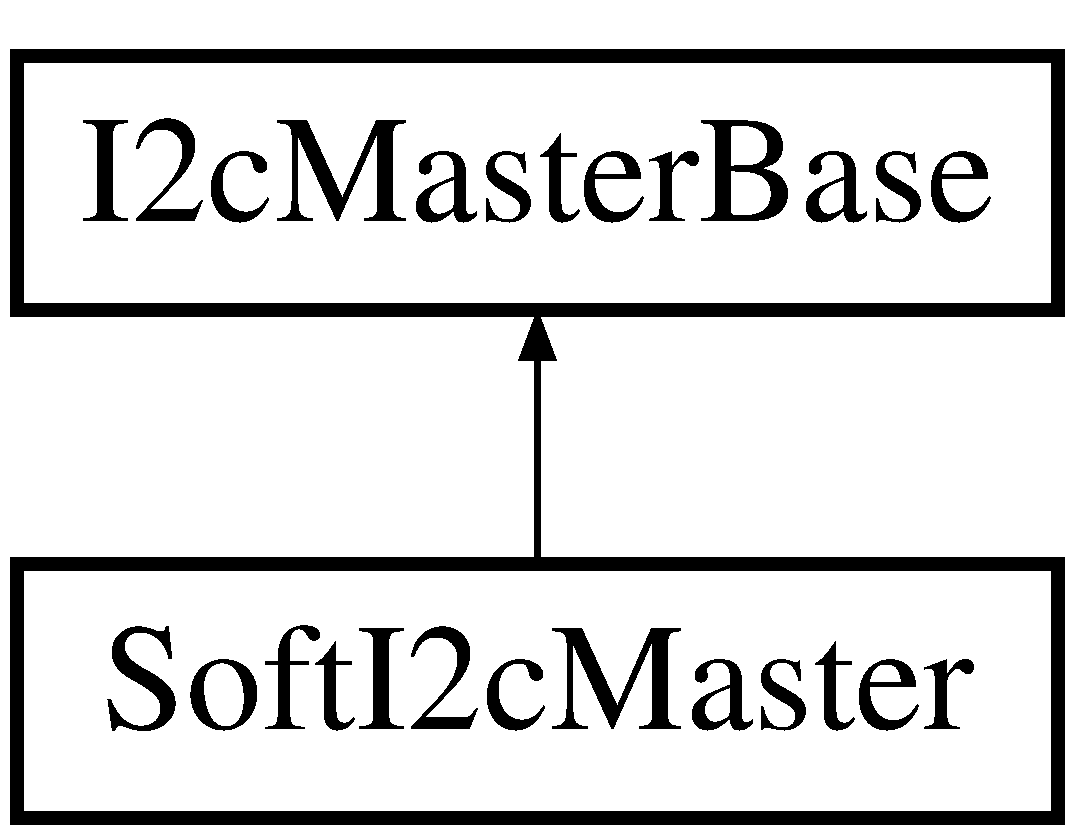
\includegraphics[height=2.000000cm]{class_i2c_master_base}
\end{center}
\end{figure}
\subsection*{Public Member Functions}
\begin{DoxyCompactItemize}
\item 
virtual uint8\+\_\+t \hyperlink{class_i2c_master_base_ab0642665deb11295592d3e46c8baaefa}{read} (uint8\+\_\+t last)=0
\item 
virtual bool \hyperlink{class_i2c_master_base_a3ccb7274e45f8842f5748d5ae9931dd0}{restart} (uint8\+\_\+t address\+R\+W)=0
\item 
virtual bool \hyperlink{class_i2c_master_base_adf5e98b79dec8f7b5a43c2ec8f2f9f7a}{start} (uint8\+\_\+t address\+R\+W)=0
\item 
virtual void \hyperlink{class_i2c_master_base_a0c4f54aea3b04ed699efc0fa684712c7}{stop} (void)=0
\item 
virtual bool \hyperlink{class_i2c_master_base_aee4d48385a72b48a0a452ecfc2cd7fc0}{write} (uint8\+\_\+t data)=0
\end{DoxyCompactItemize}


\subsection{Detailed Description}
Base class for \hyperlink{class_soft_i2c_master}{Soft\+I2c\+Master} and Twi\+Master. 

\subsection{Member Function Documentation}
\hypertarget{class_i2c_master_base_ab0642665deb11295592d3e46c8baaefa}{}\index{I2c\+Master\+Base@{I2c\+Master\+Base}!read@{read}}
\index{read@{read}!I2c\+Master\+Base@{I2c\+Master\+Base}}
\subsubsection[{read}]{\setlength{\rightskip}{0pt plus 5cm}virtual uint8\+\_\+t I2c\+Master\+Base\+::read (
\begin{DoxyParamCaption}
\item[{uint8\+\_\+t}]{last}
\end{DoxyParamCaption}
)\hspace{0.3cm}{\ttfamily [pure virtual]}}\label{class_i2c_master_base_ab0642665deb11295592d3e46c8baaefa}
Read a byte 
\begin{DoxyParams}[1]{Parameters}
\mbox{\tt in}  & {\em last} & send Ack if last is false else Nak to terminate read \\
\hline
\end{DoxyParams}
\begin{DoxyReturn}{Returns}
byte read from I2\+C bus 
\end{DoxyReturn}


Implemented in \hyperlink{class_soft_i2c_master_a56993378a66a702113eef640d8c82ea9}{Soft\+I2c\+Master}.

\hypertarget{class_i2c_master_base_a3ccb7274e45f8842f5748d5ae9931dd0}{}\index{I2c\+Master\+Base@{I2c\+Master\+Base}!restart@{restart}}
\index{restart@{restart}!I2c\+Master\+Base@{I2c\+Master\+Base}}
\subsubsection[{restart}]{\setlength{\rightskip}{0pt plus 5cm}virtual bool I2c\+Master\+Base\+::restart (
\begin{DoxyParamCaption}
\item[{uint8\+\_\+t}]{address\+R\+W}
\end{DoxyParamCaption}
)\hspace{0.3cm}{\ttfamily [pure virtual]}}\label{class_i2c_master_base_a3ccb7274e45f8842f5748d5ae9931dd0}
Send new address and read/write bit without sending a stop. 
\begin{DoxyParams}[1]{Parameters}
\mbox{\tt in}  & {\em address\+R\+W} & i2c address with read/write bit \\
\hline
\end{DoxyParams}
\begin{DoxyReturn}{Returns}
true for success false for failure 
\end{DoxyReturn}


Implemented in \hyperlink{class_soft_i2c_master_a4ec0db661a654943888df023b233bcc5}{Soft\+I2c\+Master}.

\hypertarget{class_i2c_master_base_adf5e98b79dec8f7b5a43c2ec8f2f9f7a}{}\index{I2c\+Master\+Base@{I2c\+Master\+Base}!start@{start}}
\index{start@{start}!I2c\+Master\+Base@{I2c\+Master\+Base}}
\subsubsection[{start}]{\setlength{\rightskip}{0pt plus 5cm}virtual bool I2c\+Master\+Base\+::start (
\begin{DoxyParamCaption}
\item[{uint8\+\_\+t}]{address\+R\+W}
\end{DoxyParamCaption}
)\hspace{0.3cm}{\ttfamily [pure virtual]}}\label{class_i2c_master_base_adf5e98b79dec8f7b5a43c2ec8f2f9f7a}
Issue a start condition 
\begin{DoxyParams}[1]{Parameters}
\mbox{\tt in}  & {\em address\+R\+W} & i2c address with read/write bit \\
\hline
\end{DoxyParams}
\begin{DoxyReturn}{Returns}
true for success false for failure 
\end{DoxyReturn}


Implemented in \hyperlink{class_soft_i2c_master_a66a6298702caed4f52537ef372307699}{Soft\+I2c\+Master}.

\hypertarget{class_i2c_master_base_a0c4f54aea3b04ed699efc0fa684712c7}{}\index{I2c\+Master\+Base@{I2c\+Master\+Base}!stop@{stop}}
\index{stop@{stop}!I2c\+Master\+Base@{I2c\+Master\+Base}}
\subsubsection[{stop}]{\setlength{\rightskip}{0pt plus 5cm}virtual void I2c\+Master\+Base\+::stop (
\begin{DoxyParamCaption}
\item[{void}]{}
\end{DoxyParamCaption}
)\hspace{0.3cm}{\ttfamily [pure virtual]}}\label{class_i2c_master_base_a0c4f54aea3b04ed699efc0fa684712c7}
Issue a stop condition. 

Implemented in \hyperlink{class_soft_i2c_master_ad8f52e1cbf15894472881afe439afa02}{Soft\+I2c\+Master}.

\hypertarget{class_i2c_master_base_aee4d48385a72b48a0a452ecfc2cd7fc0}{}\index{I2c\+Master\+Base@{I2c\+Master\+Base}!write@{write}}
\index{write@{write}!I2c\+Master\+Base@{I2c\+Master\+Base}}
\subsubsection[{write}]{\setlength{\rightskip}{0pt plus 5cm}virtual bool I2c\+Master\+Base\+::write (
\begin{DoxyParamCaption}
\item[{uint8\+\_\+t}]{data}
\end{DoxyParamCaption}
)\hspace{0.3cm}{\ttfamily [pure virtual]}}\label{class_i2c_master_base_aee4d48385a72b48a0a452ecfc2cd7fc0}
Write a byte 
\begin{DoxyParams}[1]{Parameters}
\mbox{\tt in}  & {\em data} & byte to write \\
\hline
\end{DoxyParams}
\begin{DoxyReturn}{Returns}
true for Ack or false for Nak 
\end{DoxyReturn}


Implemented in \hyperlink{class_soft_i2c_master_abcce5d83ae63dc61c2662be4a934d083}{Soft\+I2c\+Master}.



The documentation for this class was generated from the following file\+:\begin{DoxyCompactItemize}
\item 
Wiring/\hyperlink{_i2c_master_8h}{I2c\+Master.\+h}\end{DoxyCompactItemize}

\hypertarget{structicmp__echo__hdr}{}\section{icmp\+\_\+echo\+\_\+hdr Struct Reference}
\label{structicmp__echo__hdr}\index{icmp\+\_\+echo\+\_\+hdr@{icmp\+\_\+echo\+\_\+hdr}}


{\ttfamily \#include $<$icmp.\+h$>$}

\subsection*{Public Member Functions}
\begin{DoxyCompactItemize}
\item 
\hypertarget{structicmp__echo__hdr_a628281d8598df1d2ebc16ed59c72d1c0}{}{\bfseries P\+A\+C\+K\+\_\+\+S\+T\+R\+U\+C\+T\+\_\+\+F\+I\+E\+L\+D} (u8\+\_\+t type)\label{structicmp__echo__hdr_a628281d8598df1d2ebc16ed59c72d1c0}

\item 
\hypertarget{structicmp__echo__hdr_a05adf7444332cf0f1497b5e009b2bc3e}{}{\bfseries P\+A\+C\+K\+\_\+\+S\+T\+R\+U\+C\+T\+\_\+\+F\+I\+E\+L\+D} (u8\+\_\+t code)\label{structicmp__echo__hdr_a05adf7444332cf0f1497b5e009b2bc3e}

\item 
\hypertarget{structicmp__echo__hdr_a5d1bdfcc4a8bdd58513ecbaea368c1ad}{}{\bfseries P\+A\+C\+K\+\_\+\+S\+T\+R\+U\+C\+T\+\_\+\+F\+I\+E\+L\+D} (u16\+\_\+t chksum)\label{structicmp__echo__hdr_a5d1bdfcc4a8bdd58513ecbaea368c1ad}

\item 
\hypertarget{structicmp__echo__hdr_a35dd6758d625e1542599175e65235362}{}{\bfseries P\+A\+C\+K\+\_\+\+S\+T\+R\+U\+C\+T\+\_\+\+F\+I\+E\+L\+D} (u16\+\_\+t id)\label{structicmp__echo__hdr_a35dd6758d625e1542599175e65235362}

\item 
\hypertarget{structicmp__echo__hdr_a2d2722057bc87fa0afb495ba6716eb57}{}{\bfseries P\+A\+C\+K\+\_\+\+S\+T\+R\+U\+C\+T\+\_\+\+F\+I\+E\+L\+D} (u16\+\_\+t seqno)\label{structicmp__echo__hdr_a2d2722057bc87fa0afb495ba6716eb57}

\end{DoxyCompactItemize}


\subsection{Detailed Description}
This is the standard I\+C\+M\+P header only that the u32\+\_\+t data is splitted to two u16\+\_\+t like I\+C\+M\+P echo needs it. This header is also used for other I\+C\+M\+P types that do not use the data part. ����\+I\+C\+M\+P�����������ײ��ṹ�� ��������\+I\+C\+M\+P�����ײ��кܴ������ԣ� �ýṹͬ������������\+I\+C\+M\+P���ġ� 

The documentation for this struct was generated from the following file\+:\begin{DoxyCompactItemize}
\item 
system/include/lwip/icmp.\+h\end{DoxyCompactItemize}

\hypertarget{class_i_data_source_stream}{}\section{I\+Data\+Source\+Stream Class Reference}
\label{class_i_data_source_stream}\index{I\+Data\+Source\+Stream@{I\+Data\+Source\+Stream}}
Inheritance diagram for I\+Data\+Source\+Stream\+:\begin{figure}[H]
\begin{center}
\leavevmode
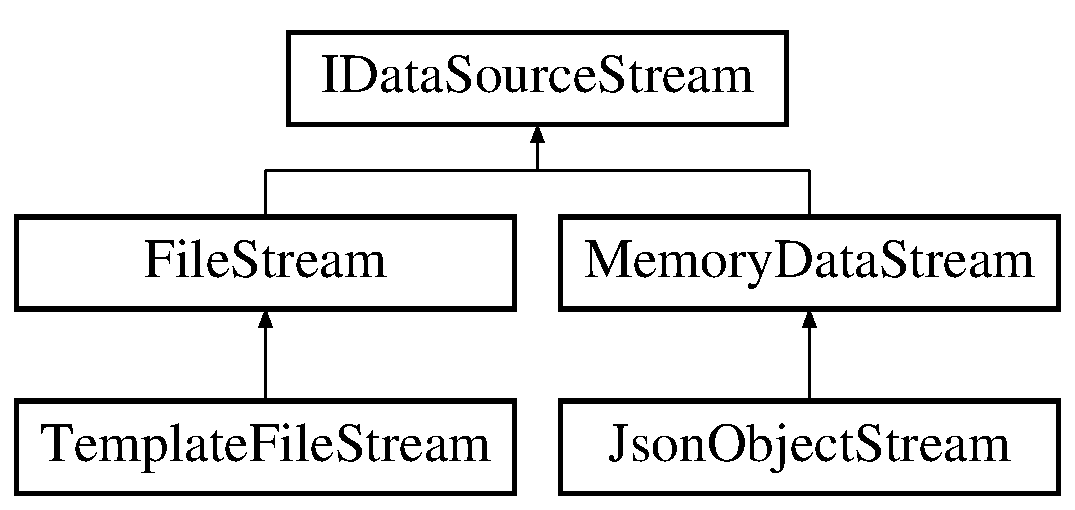
\includegraphics[height=3.000000cm]{class_i_data_source_stream}
\end{center}
\end{figure}
\subsection*{Public Member Functions}
\begin{DoxyCompactItemize}
\item 
\hypertarget{class_i_data_source_stream_a589085e0eea011acdc401b79831826e0}{}virtual Stream\+Type {\bfseries get\+Stream\+Type} ()=0\label{class_i_data_source_stream_a589085e0eea011acdc401b79831826e0}

\item 
\hypertarget{class_i_data_source_stream_ac4eacca7f55c8618a2ca52d90d6cb919}{}virtual uint16\+\_\+t {\bfseries get\+Data\+Pointer} (char $\ast$$\ast$data)=0\label{class_i_data_source_stream_ac4eacca7f55c8618a2ca52d90d6cb919}

\item 
\hypertarget{class_i_data_source_stream_a3a2c1c9c686a6c99041316dc0531c255}{}virtual bool {\bfseries seek} (int len)=0\label{class_i_data_source_stream_a3a2c1c9c686a6c99041316dc0531c255}

\item 
\hypertarget{class_i_data_source_stream_a143958f311cc98fbfaaec1d4d5cdfe47}{}virtual bool {\bfseries is\+Finished} ()=0\label{class_i_data_source_stream_a143958f311cc98fbfaaec1d4d5cdfe47}

\end{DoxyCompactItemize}


The documentation for this class was generated from the following file\+:\begin{DoxyCompactItemize}
\item 
Sming\+Core/Data\+Source\+Stream.\+h\end{DoxyCompactItemize}

\hypertarget{class_i_delegate_caller}{}\section{I\+Delegate\+Caller$<$ Return\+Type, Params\+List $>$ Class Template Reference}
\label{class_i_delegate_caller}\index{I\+Delegate\+Caller$<$ Return\+Type, Params\+List $>$@{I\+Delegate\+Caller$<$ Return\+Type, Params\+List $>$}}
\subsection*{Public Member Functions}
\begin{DoxyCompactItemize}
\item 
\hypertarget{class_i_delegate_caller_aeff22075798c3f85fed2d72b62964178}{}virtual Return\+Type {\bfseries invoke} (Params\+List...)=0\label{class_i_delegate_caller_aeff22075798c3f85fed2d72b62964178}

\item 
\hypertarget{class_i_delegate_caller_a3af9e79f473f57e8202c4973d5f37366}{}\+\_\+\+\_\+forceinline void {\bfseries increase} ()\label{class_i_delegate_caller_a3af9e79f473f57e8202c4973d5f37366}

\item 
\hypertarget{class_i_delegate_caller_a4c49d3a30a5224c1910400b9a1cbaf71}{}\+\_\+\+\_\+forceinline void {\bfseries decrease} ()\label{class_i_delegate_caller_a4c49d3a30a5224c1910400b9a1cbaf71}

\end{DoxyCompactItemize}


The documentation for this class was generated from the following file\+:\begin{DoxyCompactItemize}
\item 
Sming\+Core/Delegate.\+h\end{DoxyCompactItemize}

\hypertarget{structin__addr}{}\section{in\+\_\+addr Struct Reference}
\label{structin__addr}\index{in\+\_\+addr@{in\+\_\+addr}}


{\ttfamily \#include $<$inet.\+h$>$}

\subsection*{Public Attributes}
\begin{DoxyCompactItemize}
\item 
\hypertarget{structin__addr_a0c76d44232bae90455a5189b32a9b625}{}u32\+\_\+t {\bfseries s\+\_\+addr}\label{structin__addr_a0c76d44232bae90455a5189b32a9b625}

\end{DoxyCompactItemize}


\subsection{Detailed Description}
For compatibility with B\+S\+D code 

The documentation for this struct was generated from the following file\+:\begin{DoxyCompactItemize}
\item 
system/include/lwip/inet.\+h\end{DoxyCompactItemize}

\hypertarget{class_arduino_json_1_1_internals_1_1_indented_print}{}\section{Arduino\+Json\+:\+:Internals\+:\+:Indented\+Print Class Reference}
\label{class_arduino_json_1_1_internals_1_1_indented_print}\index{Arduino\+Json\+::\+Internals\+::\+Indented\+Print@{Arduino\+Json\+::\+Internals\+::\+Indented\+Print}}
Inheritance diagram for Arduino\+Json\+:\+:Internals\+:\+:Indented\+Print\+:\begin{figure}[H]
\begin{center}
\leavevmode
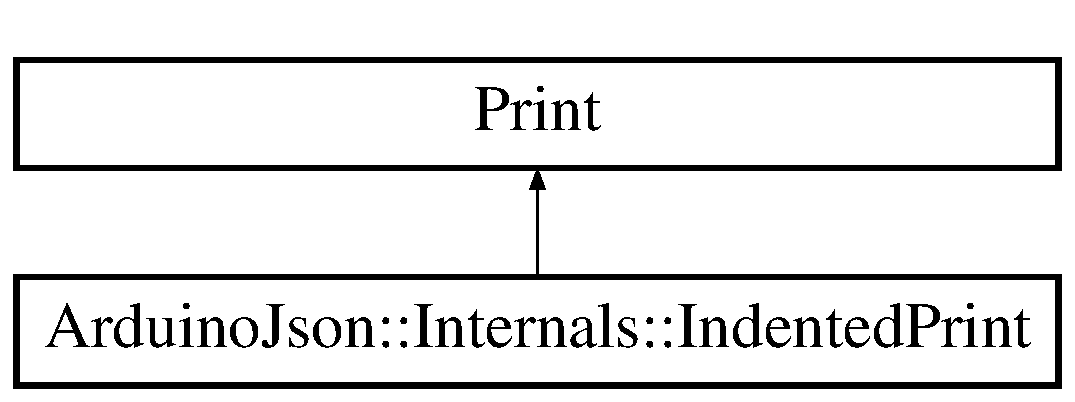
\includegraphics[height=2.000000cm]{class_arduino_json_1_1_internals_1_1_indented_print}
\end{center}
\end{figure}
\subsection*{Public Member Functions}
\begin{DoxyCompactItemize}
\item 
\hypertarget{class_arduino_json_1_1_internals_1_1_indented_print_aa408b0c0bcb59f5f23dfba262ddca687}{}{\bfseries Indented\+Print} (Print \&p)\label{class_arduino_json_1_1_internals_1_1_indented_print_aa408b0c0bcb59f5f23dfba262ddca687}

\item 
\hypertarget{class_arduino_json_1_1_internals_1_1_indented_print_a93fda715afb45824a25c6df1b9bd77c1}{}virtual size\+\_\+t {\bfseries write} (uint8\+\_\+t)\label{class_arduino_json_1_1_internals_1_1_indented_print_a93fda715afb45824a25c6df1b9bd77c1}

\item 
\hypertarget{class_arduino_json_1_1_internals_1_1_indented_print_ab9530073fcda29015ecfdd5b93c884f3}{}void {\bfseries indent} ()\label{class_arduino_json_1_1_internals_1_1_indented_print_ab9530073fcda29015ecfdd5b93c884f3}

\item 
\hypertarget{class_arduino_json_1_1_internals_1_1_indented_print_aeb112bb656fbfef91bc2d9450b5b673b}{}void {\bfseries unindent} ()\label{class_arduino_json_1_1_internals_1_1_indented_print_aeb112bb656fbfef91bc2d9450b5b673b}

\item 
\hypertarget{class_arduino_json_1_1_internals_1_1_indented_print_aaed75d4165b3cc46619a893de252c486}{}void {\bfseries set\+Tab\+Size} (uint8\+\_\+t n)\label{class_arduino_json_1_1_internals_1_1_indented_print_aaed75d4165b3cc46619a893de252c486}

\end{DoxyCompactItemize}


The documentation for this class was generated from the following files\+:\begin{DoxyCompactItemize}
\item 
Services/\+Arduino\+Json/include/\+Arduino\+Json/\+Internals/Indented\+Print.\+hpp\item 
Services/\+Arduino\+Json/src/\+Internals/Indented\+Print.\+cpp\end{DoxyCompactItemize}

\hypertarget{structip__addr}{}\section{ip\+\_\+addr Struct Reference}
\label{structip__addr}\index{ip\+\_\+addr@{ip\+\_\+addr}}
\subsection*{Public Attributes}
\begin{DoxyCompactItemize}
\item 
\hypertarget{structip__addr_ae21beaba54c79518c4b77b279f744c21}{}u32\+\_\+t {\bfseries addr}\label{structip__addr_ae21beaba54c79518c4b77b279f744c21}

\end{DoxyCompactItemize}


The documentation for this struct was generated from the following file\+:\begin{DoxyCompactItemize}
\item 
system/include/lwip/ip\+\_\+addr.\+h\end{DoxyCompactItemize}

\hypertarget{structip__addr2}{}\section{ip\+\_\+addr2 Struct Reference}
\label{structip__addr2}\index{ip\+\_\+addr2@{ip\+\_\+addr2}}
\subsection*{Public Member Functions}
\begin{DoxyCompactItemize}
\item 
\hypertarget{structip__addr2_a098e42efa61e0c431ab501098426767d}{}{\bfseries P\+A\+C\+K\+\_\+\+S\+T\+R\+U\+C\+T\+\_\+\+F\+I\+E\+L\+D} (u16\+\_\+t addrw\mbox{[}2\mbox{]})\label{structip__addr2_a098e42efa61e0c431ab501098426767d}

\end{DoxyCompactItemize}


The documentation for this struct was generated from the following file\+:\begin{DoxyCompactItemize}
\item 
system/include/lwip/ip\+\_\+addr.\+h\end{DoxyCompactItemize}

\hypertarget{structip__addr__packed}{}\section{ip\+\_\+addr\+\_\+packed Struct Reference}
\label{structip__addr__packed}\index{ip\+\_\+addr\+\_\+packed@{ip\+\_\+addr\+\_\+packed}}
\subsection*{Public Member Functions}
\begin{DoxyCompactItemize}
\item 
\hypertarget{structip__addr__packed_ad9a337a45101464bb2e6e54c5b0292de}{}{\bfseries P\+A\+C\+K\+\_\+\+S\+T\+R\+U\+C\+T\+\_\+\+F\+I\+E\+L\+D} (u32\+\_\+t addr)\label{structip__addr__packed_ad9a337a45101464bb2e6e54c5b0292de}

\end{DoxyCompactItemize}


The documentation for this struct was generated from the following file\+:\begin{DoxyCompactItemize}
\item 
system/include/lwip/ip\+\_\+addr.\+h\end{DoxyCompactItemize}

\hypertarget{structip__hdr}{}\section{ip\+\_\+hdr Struct Reference}
\label{structip__hdr}\index{ip\+\_\+hdr@{ip\+\_\+hdr}}
\subsection*{Public Member Functions}
\begin{DoxyCompactItemize}
\item 
\hypertarget{structip__hdr_a10524f0bebe44c882756c05e67ad9bfd}{}{\bfseries P\+A\+C\+K\+\_\+\+S\+T\+R\+U\+C\+T\+\_\+\+F\+I\+E\+L\+D} (u16\+\_\+t \+\_\+v\+\_\+hl\+\_\+tos)\label{structip__hdr_a10524f0bebe44c882756c05e67ad9bfd}

\item 
\hypertarget{structip__hdr_aa3905f2613b3ce0994d3a04cf22ce2d7}{}{\bfseries P\+A\+C\+K\+\_\+\+S\+T\+R\+U\+C\+T\+\_\+\+F\+I\+E\+L\+D} (u16\+\_\+t \+\_\+len)\label{structip__hdr_aa3905f2613b3ce0994d3a04cf22ce2d7}

\item 
\hypertarget{structip__hdr_a6d3aca5e6bdd354c377836c67d93575b}{}{\bfseries P\+A\+C\+K\+\_\+\+S\+T\+R\+U\+C\+T\+\_\+\+F\+I\+E\+L\+D} (u16\+\_\+t \+\_\+id)\label{structip__hdr_a6d3aca5e6bdd354c377836c67d93575b}

\item 
\hypertarget{structip__hdr_a2c93d9f414cb5e3bd727799393b3688a}{}{\bfseries P\+A\+C\+K\+\_\+\+S\+T\+R\+U\+C\+T\+\_\+\+F\+I\+E\+L\+D} (u16\+\_\+t \+\_\+offset)\label{structip__hdr_a2c93d9f414cb5e3bd727799393b3688a}

\item 
\hypertarget{structip__hdr_a0d402789ed4488b5538e276b117bfbd1}{}{\bfseries P\+A\+C\+K\+\_\+\+S\+T\+R\+U\+C\+T\+\_\+\+F\+I\+E\+L\+D} (u8\+\_\+t \+\_\+ttl)\label{structip__hdr_a0d402789ed4488b5538e276b117bfbd1}

\item 
\hypertarget{structip__hdr_a4fb16bde7f441a14cc673fe12289153f}{}{\bfseries P\+A\+C\+K\+\_\+\+S\+T\+R\+U\+C\+T\+\_\+\+F\+I\+E\+L\+D} (u8\+\_\+t \+\_\+proto)\label{structip__hdr_a4fb16bde7f441a14cc673fe12289153f}

\item 
\hypertarget{structip__hdr_a620275dbd7f7b8f02cf3f90fa035eb62}{}{\bfseries P\+A\+C\+K\+\_\+\+S\+T\+R\+U\+C\+T\+\_\+\+F\+I\+E\+L\+D} (u16\+\_\+t \+\_\+chksum)\label{structip__hdr_a620275dbd7f7b8f02cf3f90fa035eb62}

\item 
\hypertarget{structip__hdr_a5d6152fc140e12c611356c54147e91e1}{}{\bfseries P\+A\+C\+K\+\_\+\+S\+T\+R\+U\+C\+T\+\_\+\+F\+I\+E\+L\+D} (\hyperlink{structip__addr__packed}{ip\+\_\+addr\+\_\+p\+\_\+t} src)\label{structip__hdr_a5d6152fc140e12c611356c54147e91e1}

\item 
\hypertarget{structip__hdr_a7e0bc4d66ad8a63251fd83c7168077a3}{}{\bfseries P\+A\+C\+K\+\_\+\+S\+T\+R\+U\+C\+T\+\_\+\+F\+I\+E\+L\+D} (\hyperlink{structip__addr__packed}{ip\+\_\+addr\+\_\+p\+\_\+t} dest)\label{structip__hdr_a7e0bc4d66ad8a63251fd83c7168077a3}

\end{DoxyCompactItemize}


The documentation for this struct was generated from the following file\+:\begin{DoxyCompactItemize}
\item 
system/include/lwip/ip.\+h\end{DoxyCompactItemize}

\hypertarget{structip__info}{}\section{ip\+\_\+info Struct Reference}
\label{structip__info}\index{ip\+\_\+info@{ip\+\_\+info}}
\subsection*{Public Attributes}
\begin{DoxyCompactItemize}
\item 
\hypertarget{structip__info_a4936657e519be54caf19352b23846913}{}struct \hyperlink{structip__addr}{ip\+\_\+addr} {\bfseries ip}\label{structip__info_a4936657e519be54caf19352b23846913}

\item 
\hypertarget{structip__info_a3f9e6d30f4ec10eefa7b51653e5c3da4}{}struct \hyperlink{structip__addr}{ip\+\_\+addr} {\bfseries netmask}\label{structip__info_a3f9e6d30f4ec10eefa7b51653e5c3da4}

\item 
\hypertarget{structip__info_a688311148a7415577157c439ee77ee0b}{}struct \hyperlink{structip__addr}{ip\+\_\+addr} {\bfseries gw}\label{structip__info_a688311148a7415577157c439ee77ee0b}

\end{DoxyCompactItemize}


The documentation for this struct was generated from the following file\+:\begin{DoxyCompactItemize}
\item 
system/include/lwip/ip\+\_\+addr.\+h\end{DoxyCompactItemize}

\hypertarget{structip__pcb}{}\section{ip\+\_\+pcb Struct Reference}
\label{structip__pcb}\index{ip\+\_\+pcb@{ip\+\_\+pcb}}
\subsection*{Public Attributes}
\begin{DoxyCompactItemize}
\item 
\hypertarget{structip__pcb_aa8c53363aec905c3556c4ce197e24fc3}{}{\bfseries I\+P\+\_\+\+P\+C\+B}\label{structip__pcb_aa8c53363aec905c3556c4ce197e24fc3}

\end{DoxyCompactItemize}


The documentation for this struct was generated from the following file\+:\begin{DoxyCompactItemize}
\item 
system/include/lwip/ip.\+h\end{DoxyCompactItemize}

\hypertarget{class_i_p_address}{}\section{I\+P\+Address Class Reference}
\label{class_i_p_address}\index{I\+P\+Address@{I\+P\+Address}}
Inheritance diagram for I\+P\+Address\+:\begin{figure}[H]
\begin{center}
\leavevmode
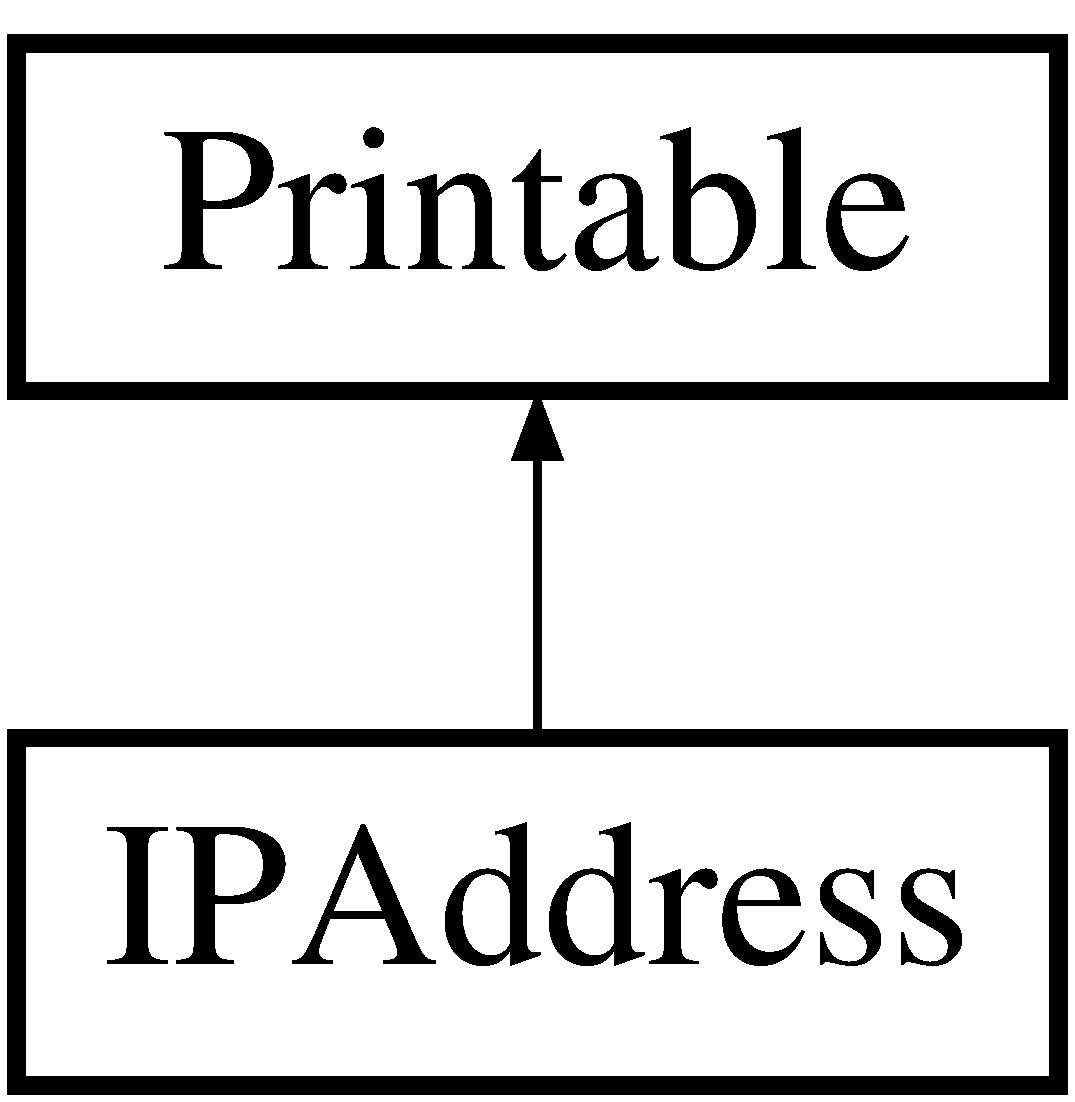
\includegraphics[height=2.000000cm]{class_i_p_address}
\end{center}
\end{figure}
\subsection*{Public Member Functions}
\begin{DoxyCompactItemize}
\item 
\hypertarget{class_i_p_address_af25acf9a16981a1b95c66e9e683245b0}{}{\bfseries I\+P\+Address} (uint8\+\_\+t first\+\_\+octet, uint8\+\_\+t second\+\_\+octet, uint8\+\_\+t third\+\_\+octet, uint8\+\_\+t fourth\+\_\+octet)\label{class_i_p_address_af25acf9a16981a1b95c66e9e683245b0}

\item 
\hypertarget{class_i_p_address_a9acd9971a8fc47fa51681e9b9a95b511}{}{\bfseries I\+P\+Address} (uint32\+\_\+t address)\label{class_i_p_address_a9acd9971a8fc47fa51681e9b9a95b511}

\item 
\hypertarget{class_i_p_address_a41fef26d1776762bb1e25cd23278ada8}{}{\bfseries I\+P\+Address} (\hyperlink{structip__addr}{ip\+\_\+addr} address)\label{class_i_p_address_a41fef26d1776762bb1e25cd23278ada8}

\item 
\hypertarget{class_i_p_address_ab747742c0a428a369f6ab73b7d28c306}{}{\bfseries I\+P\+Address} (const uint8\+\_\+t $\ast$address)\label{class_i_p_address_ab747742c0a428a369f6ab73b7d28c306}

\item 
\hypertarget{class_i_p_address_afb9b73e257da0169b7ffcb5d8122a9f7}{}{\bfseries I\+P\+Address} (const String address)\label{class_i_p_address_afb9b73e257da0169b7ffcb5d8122a9f7}

\item 
\hypertarget{class_i_p_address_a90aebdb7f5f655fe3a5e3d8aa3bc3ac8}{}{\bfseries operator uint32\+\_\+t} ()\label{class_i_p_address_a90aebdb7f5f655fe3a5e3d8aa3bc3ac8}

\item 
\hypertarget{class_i_p_address_a5e05f9ca93074e4413225a70bda15174}{}{\bfseries operator ip\+\_\+addr} ()\label{class_i_p_address_a5e05f9ca93074e4413225a70bda15174}

\item 
\hypertarget{class_i_p_address_a99483365155bf097dd937594b372cf04}{}{\bfseries operator ip\+\_\+addr $\ast$} ()\label{class_i_p_address_a99483365155bf097dd937594b372cf04}

\item 
\hypertarget{class_i_p_address_adc404569f7c8193c1be9d79a27753099}{}bool {\bfseries operator==} (const \hyperlink{class_i_p_address}{I\+P\+Address} \&addr)\label{class_i_p_address_adc404569f7c8193c1be9d79a27753099}

\item 
\hypertarget{class_i_p_address_af685847e3b72825b9c9f0ed5b828683f}{}bool {\bfseries operator==} (const uint8\+\_\+t $\ast$addr)\label{class_i_p_address_af685847e3b72825b9c9f0ed5b828683f}

\item 
\hypertarget{class_i_p_address_a25dd61caa38bb38961f982406fddceea}{}bool {\bfseries is\+Null} ()\label{class_i_p_address_a25dd61caa38bb38961f982406fddceea}

\item 
\hypertarget{class_i_p_address_af00071ac24a5ed453e323f1535c9f33c}{}String {\bfseries to\+String} ()\label{class_i_p_address_af00071ac24a5ed453e323f1535c9f33c}

\item 
\hypertarget{class_i_p_address_ac1e9d3628dc5bc5151324c80a69ad159}{}uint8\+\_\+t {\bfseries operator\mbox{[}$\,$\mbox{]}} (int index) const \label{class_i_p_address_ac1e9d3628dc5bc5151324c80a69ad159}

\item 
\hypertarget{class_i_p_address_ab7c569a71648e9235ebb63d7a6d58143}{}uint8\+\_\+t \& {\bfseries operator\mbox{[}$\,$\mbox{]}} (int index)\label{class_i_p_address_ab7c569a71648e9235ebb63d7a6d58143}

\item 
\hypertarget{class_i_p_address_a0dc5d0937fec535ef61daa5d05f30d3a}{}\hyperlink{class_i_p_address}{I\+P\+Address} \& {\bfseries operator=} (const uint8\+\_\+t $\ast$address)\label{class_i_p_address_a0dc5d0937fec535ef61daa5d05f30d3a}

\item 
\hypertarget{class_i_p_address_af80a0f81dc5861ae3240a4331c5fc14c}{}\hyperlink{class_i_p_address}{I\+P\+Address} \& {\bfseries operator=} (uint32\+\_\+t address)\label{class_i_p_address_af80a0f81dc5861ae3240a4331c5fc14c}

\item 
\hypertarget{class_i_p_address_aea4405da8c3a18834d97c1afacb73875}{}\hyperlink{class_i_p_address}{I\+P\+Address} \& {\bfseries operator=} (const String address)\label{class_i_p_address_aea4405da8c3a18834d97c1afacb73875}

\item 
\hypertarget{class_i_p_address_a2dd7f6c455c2f33e4639944f751930db}{}virtual size\+\_\+t {\bfseries print\+To} (Print \&p) const \label{class_i_p_address_a2dd7f6c455c2f33e4639944f751930db}

\end{DoxyCompactItemize}


The documentation for this class was generated from the following files\+:\begin{DoxyCompactItemize}
\item 
Wiring/I\+P\+Address.\+h\item 
Wiring/I\+P\+Address.\+cpp\end{DoxyCompactItemize}

\hypertarget{class_i_system_ready_handler}{}\section{I\+System\+Ready\+Handler Class Reference}
\label{class_i_system_ready_handler}\index{I\+System\+Ready\+Handler@{I\+System\+Ready\+Handler}}
Inheritance diagram for I\+System\+Ready\+Handler\+:\begin{figure}[H]
\begin{center}
\leavevmode
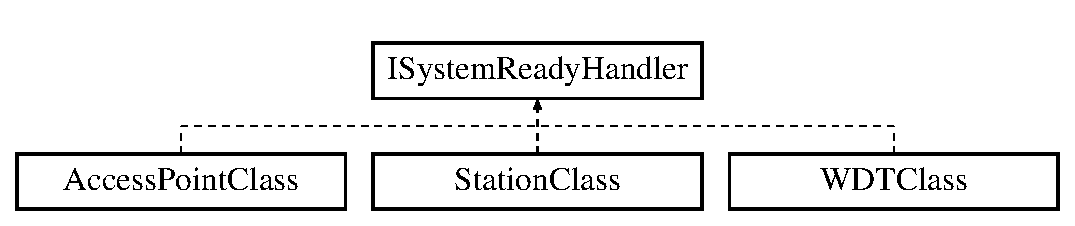
\includegraphics[height=2.000000cm]{class_i_system_ready_handler}
\end{center}
\end{figure}
\subsection*{Public Member Functions}
\begin{DoxyCompactItemize}
\item 
\hypertarget{class_i_system_ready_handler_ae52e11b1a352b6d66490ac912bf10be4}{}virtual void {\bfseries on\+System\+Ready} ()=0\label{class_i_system_ready_handler_ae52e11b1a352b6d66490ac912bf10be4}

\end{DoxyCompactItemize}


The documentation for this class was generated from the following file\+:\begin{DoxyCompactItemize}
\item 
Sming\+Core/\+Platform/System.\+h\end{DoxyCompactItemize}

\hypertarget{class_arduino_json_1_1_json_array}{}\section{Arduino\+Json\+:\+:Json\+Array Class Reference}
\label{class_arduino_json_1_1_json_array}\index{Arduino\+Json\+::\+Json\+Array@{Arduino\+Json\+::\+Json\+Array}}
Inheritance diagram for Arduino\+Json\+:\+:Json\+Array\+:\begin{figure}[H]
\begin{center}
\leavevmode
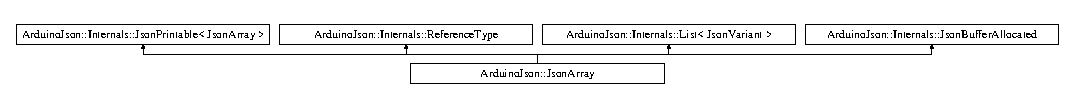
\includegraphics[height=0.894569cm]{class_arduino_json_1_1_json_array}
\end{center}
\end{figure}
\subsection*{Public Member Functions}
\begin{DoxyCompactItemize}
\item 
\hypertarget{class_arduino_json_1_1_json_array_adc4cb692a95942dfae731345d646212e}{}\hyperlink{class_arduino_json_1_1_json_variant}{Json\+Variant} \& {\bfseries at} (int index) const \label{class_arduino_json_1_1_json_array_adc4cb692a95942dfae731345d646212e}

\item 
\hypertarget{class_arduino_json_1_1_json_array_a87f9ea8e71b249daa31ff3ce6fb559fc}{}\hyperlink{class_arduino_json_1_1_json_variant}{Json\+Variant} \& {\bfseries operator\mbox{[}$\,$\mbox{]}} (int index) const \label{class_arduino_json_1_1_json_array_a87f9ea8e71b249daa31ff3ce6fb559fc}

\item 
\hypertarget{class_arduino_json_1_1_json_array_af2e2390085a2bf56c6b662d133a21ec1}{}\hyperlink{class_arduino_json_1_1_json_variant}{Json\+Variant} \& {\bfseries add} ()\label{class_arduino_json_1_1_json_array_af2e2390085a2bf56c6b662d133a21ec1}

\item 
\hypertarget{class_arduino_json_1_1_json_array_ad5b9bd2e9708bf30627c6c9fc013f92f}{}{\footnotesize template$<$typename T $>$ }\\void {\bfseries add} (T value)\label{class_arduino_json_1_1_json_array_ad5b9bd2e9708bf30627c6c9fc013f92f}

\item 
\hypertarget{class_arduino_json_1_1_json_array_a5765cac60aed5cd22d765c21fda94b1f}{}void {\bfseries add} (double value, uint8\+\_\+t decimals)\label{class_arduino_json_1_1_json_array_a5765cac60aed5cd22d765c21fda94b1f}

\item 
\hypertarget{class_arduino_json_1_1_json_array_aa3abbf91cf85c060a850017ac9338f27}{}void {\bfseries add} (\hyperlink{class_arduino_json_1_1_json_array}{Json\+Array} \&array)\label{class_arduino_json_1_1_json_array_aa3abbf91cf85c060a850017ac9338f27}

\item 
\hypertarget{class_arduino_json_1_1_json_array_a40ee07df289e336b1b87e047efbc265e}{}void {\bfseries add} (\hyperlink{class_arduino_json_1_1_json_object}{Json\+Object} \&obejct)\label{class_arduino_json_1_1_json_array_a40ee07df289e336b1b87e047efbc265e}

\item 
\hypertarget{class_arduino_json_1_1_json_array_acc8516b47020fe7f12028f5d29a327dd}{}void {\bfseries add} (const String \&string\+Val)\label{class_arduino_json_1_1_json_array_acc8516b47020fe7f12028f5d29a327dd}

\item 
\hypertarget{class_arduino_json_1_1_json_array_ae835359973b4efb09b6b18eccd8848f5}{}\hyperlink{class_arduino_json_1_1_json_array}{Json\+Array} \& {\bfseries create\+Nested\+Array} ()\label{class_arduino_json_1_1_json_array_ae835359973b4efb09b6b18eccd8848f5}

\item 
\hypertarget{class_arduino_json_1_1_json_array_aff022ed8518977c6dd9cf4251934c611}{}\hyperlink{class_arduino_json_1_1_json_object}{Json\+Object} \& {\bfseries create\+Nested\+Object} ()\label{class_arduino_json_1_1_json_array_aff022ed8518977c6dd9cf4251934c611}

\item 
\hypertarget{class_arduino_json_1_1_json_array_a92e011c1f231a216d32638bf0d172fe6}{}void {\bfseries write\+To} (\hyperlink{class_arduino_json_1_1_internals_1_1_json_writer}{Internals\+::\+Json\+Writer} \&writer) const \label{class_arduino_json_1_1_json_array_a92e011c1f231a216d32638bf0d172fe6}

\end{DoxyCompactItemize}
\subsection*{Static Public Member Functions}
\begin{DoxyCompactItemize}
\item 
\hypertarget{class_arduino_json_1_1_json_array_aa4d2a01145e33b5ee0c16c6b566fa08f}{}static \hyperlink{class_arduino_json_1_1_json_array}{Json\+Array} \& {\bfseries invalid} ()\label{class_arduino_json_1_1_json_array_aa4d2a01145e33b5ee0c16c6b566fa08f}

\end{DoxyCompactItemize}
\subsection*{Friends}
\begin{DoxyCompactItemize}
\item 
\hypertarget{class_arduino_json_1_1_json_array_a722362d1283cdffdf5309ff09cc998cd}{}class {\bfseries Json\+Buffer}\label{class_arduino_json_1_1_json_array_a722362d1283cdffdf5309ff09cc998cd}

\end{DoxyCompactItemize}
\subsection*{Additional Inherited Members}


The documentation for this class was generated from the following files\+:\begin{DoxyCompactItemize}
\item 
Services/\+Arduino\+Json/include/\+Arduino\+Json/Json\+Array.\+hpp\item 
Services/\+Arduino\+Json/src/Json\+Array.\+cpp\end{DoxyCompactItemize}

\hypertarget{class_arduino_json_1_1_json_buffer}{}\section{Arduino\+Json\+:\+:Json\+Buffer Class Reference}
\label{class_arduino_json_1_1_json_buffer}\index{Arduino\+Json\+::\+Json\+Buffer@{Arduino\+Json\+::\+Json\+Buffer}}
Inheritance diagram for Arduino\+Json\+:\+:Json\+Buffer\+:\begin{figure}[H]
\begin{center}
\leavevmode
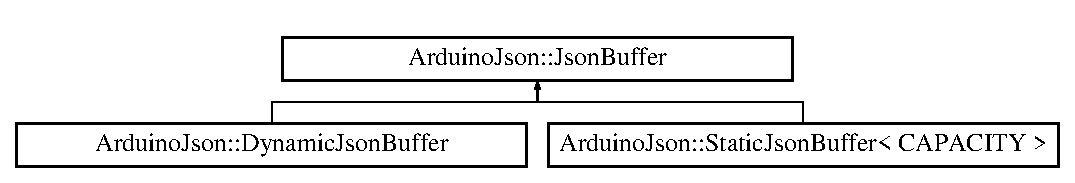
\includegraphics[height=2.000000cm]{class_arduino_json_1_1_json_buffer}
\end{center}
\end{figure}
\subsection*{Public Member Functions}
\begin{DoxyCompactItemize}
\item 
\hypertarget{class_arduino_json_1_1_json_buffer_aa51dc71ceab5bae1d78cfb78ef653a7e}{}\hyperlink{class_arduino_json_1_1_json_array}{Json\+Array} \& {\bfseries create\+Array} ()\label{class_arduino_json_1_1_json_buffer_aa51dc71ceab5bae1d78cfb78ef653a7e}

\item 
\hypertarget{class_arduino_json_1_1_json_buffer_a4a194d090e4175993aa0adb0d5fc8a85}{}\hyperlink{class_arduino_json_1_1_json_object}{Json\+Object} \& {\bfseries create\+Object} ()\label{class_arduino_json_1_1_json_buffer_a4a194d090e4175993aa0adb0d5fc8a85}

\item 
\hypertarget{class_arduino_json_1_1_json_buffer_a8e840e79b38d104ea6151427c82f0f2c}{}\hyperlink{class_arduino_json_1_1_json_array}{Json\+Array} \& {\bfseries parse\+Array} (char $\ast$json, uint8\+\_\+t nesting\+Limit=D\+E\+F\+A\+U\+L\+T\+\_\+\+L\+I\+M\+I\+T)\label{class_arduino_json_1_1_json_buffer_a8e840e79b38d104ea6151427c82f0f2c}

\item 
\hypertarget{class_arduino_json_1_1_json_buffer_a15ea1e1a8644fafcc955cc5fee880756}{}\hyperlink{class_arduino_json_1_1_json_object}{Json\+Object} \& {\bfseries parse\+Object} (char $\ast$json, uint8\+\_\+t nesting\+Limit=D\+E\+F\+A\+U\+L\+T\+\_\+\+L\+I\+M\+I\+T)\label{class_arduino_json_1_1_json_buffer_a15ea1e1a8644fafcc955cc5fee880756}

\item 
\hypertarget{class_arduino_json_1_1_json_buffer_a21d090da29ebf303815d11d6dc669d50}{}virtual void $\ast$ {\bfseries alloc} (size\+\_\+t size)=0\label{class_arduino_json_1_1_json_buffer_a21d090da29ebf303815d11d6dc669d50}

\end{DoxyCompactItemize}
\subsection*{Static Public Attributes}
\begin{DoxyCompactItemize}
\item 
\hypertarget{class_arduino_json_1_1_json_buffer_a8c353599e7f2efbc0f4c5b156918a712}{}static const uint8\+\_\+t {\bfseries D\+E\+F\+A\+U\+L\+T\+\_\+\+L\+I\+M\+I\+T} = 10\label{class_arduino_json_1_1_json_buffer_a8c353599e7f2efbc0f4c5b156918a712}

\end{DoxyCompactItemize}


The documentation for this class was generated from the following files\+:\begin{DoxyCompactItemize}
\item 
Services/\+Arduino\+Json/include/\+Arduino\+Json/Json\+Buffer.\+hpp\item 
Services/\+Arduino\+Json/src/Json\+Buffer.\+cpp\end{DoxyCompactItemize}

\hypertarget{class_arduino_json_1_1_internals_1_1_json_buffer_allocated}{}\section{Arduino\+Json\+:\+:Internals\+:\+:Json\+Buffer\+Allocated Class Reference}
\label{class_arduino_json_1_1_internals_1_1_json_buffer_allocated}\index{Arduino\+Json\+::\+Internals\+::\+Json\+Buffer\+Allocated@{Arduino\+Json\+::\+Internals\+::\+Json\+Buffer\+Allocated}}
Inheritance diagram for Arduino\+Json\+:\+:Internals\+:\+:Json\+Buffer\+Allocated\+:\begin{figure}[H]
\begin{center}
\leavevmode
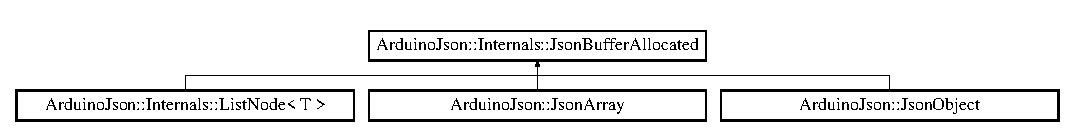
\includegraphics[height=1.398252cm]{class_arduino_json_1_1_internals_1_1_json_buffer_allocated}
\end{center}
\end{figure}
\subsection*{Public Member Functions}
\begin{DoxyCompactItemize}
\item 
\hypertarget{class_arduino_json_1_1_internals_1_1_json_buffer_allocated_afbcc0189d85cc4969991b6dc41276fb1}{}void $\ast$ {\bfseries operator new} (size\+\_\+t n, \hyperlink{class_arduino_json_1_1_json_buffer}{Json\+Buffer} $\ast$json\+Buffer)  throw ()\label{class_arduino_json_1_1_internals_1_1_json_buffer_allocated_afbcc0189d85cc4969991b6dc41276fb1}

\item 
\hypertarget{class_arduino_json_1_1_internals_1_1_json_buffer_allocated_ab1ac3cddbf84578fd87c339cb3967f25}{}void {\bfseries operator delete} (void $\ast$, \hyperlink{class_arduino_json_1_1_json_buffer}{Json\+Buffer} $\ast$)  throw ()\label{class_arduino_json_1_1_internals_1_1_json_buffer_allocated_ab1ac3cddbf84578fd87c339cb3967f25}

\end{DoxyCompactItemize}


The documentation for this class was generated from the following file\+:\begin{DoxyCompactItemize}
\item 
Services/\+Arduino\+Json/include/\+Arduino\+Json/\+Internals/Json\+Buffer\+Allocated.\+hpp\end{DoxyCompactItemize}

\hypertarget{class_arduino_json_1_1_json_object}{}\section{Arduino\+Json\+:\+:Json\+Object Class Reference}
\label{class_arduino_json_1_1_json_object}\index{Arduino\+Json\+::\+Json\+Object@{Arduino\+Json\+::\+Json\+Object}}
Inheritance diagram for Arduino\+Json\+:\+:Json\+Object\+:\begin{figure}[H]
\begin{center}
\leavevmode
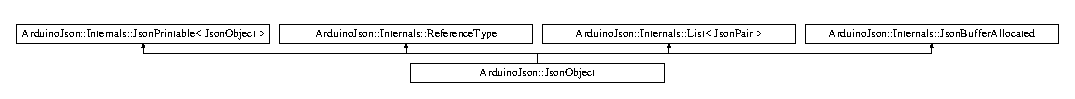
\includegraphics[height=0.883281cm]{class_arduino_json_1_1_json_object}
\end{center}
\end{figure}
\subsection*{Public Types}
\begin{DoxyCompactItemize}
\item 
\hypertarget{class_arduino_json_1_1_json_object_a848d74f26763c6de0cff7a74916caf3b}{}typedef const char $\ast$ {\bfseries key\+\_\+type}\label{class_arduino_json_1_1_json_object_a848d74f26763c6de0cff7a74916caf3b}

\item 
\hypertarget{class_arduino_json_1_1_json_object_ac999e99e637548a25aceef530b0a2e3b}{}typedef \hyperlink{struct_arduino_json_1_1_json_pair}{Json\+Pair} {\bfseries value\+\_\+type}\label{class_arduino_json_1_1_json_object_ac999e99e637548a25aceef530b0a2e3b}

\end{DoxyCompactItemize}
\subsection*{Public Member Functions}
\begin{DoxyCompactItemize}
\item 
\hypertarget{class_arduino_json_1_1_json_object_a0fbdca087f954401040f1193859c0b1c}{}\hyperlink{class_arduino_json_1_1_json_variant}{Json\+Variant} \& {\bfseries at} (key\+\_\+type key)\label{class_arduino_json_1_1_json_object_a0fbdca087f954401040f1193859c0b1c}

\item 
\hypertarget{class_arduino_json_1_1_json_object_a9e4bbb0e9194c7ae721d2d3136c1a5c3}{}const \hyperlink{class_arduino_json_1_1_json_variant}{Json\+Variant} \& {\bfseries at} (key\+\_\+type key) const \label{class_arduino_json_1_1_json_object_a9e4bbb0e9194c7ae721d2d3136c1a5c3}

\item 
\hypertarget{class_arduino_json_1_1_json_object_a027690ac3907d62f353cef1bbf320b7d}{}\hyperlink{class_arduino_json_1_1_json_variant}{Json\+Variant} \& {\bfseries operator\mbox{[}$\,$\mbox{]}} (key\+\_\+type key)\label{class_arduino_json_1_1_json_object_a027690ac3907d62f353cef1bbf320b7d}

\item 
\hypertarget{class_arduino_json_1_1_json_object_ac8b89a3f8303a09fd00c7b2fd40ccf91}{}const \hyperlink{class_arduino_json_1_1_json_variant}{Json\+Variant} \& {\bfseries operator\mbox{[}$\,$\mbox{]}} (key\+\_\+type key) const \label{class_arduino_json_1_1_json_object_ac8b89a3f8303a09fd00c7b2fd40ccf91}

\item 
\hypertarget{class_arduino_json_1_1_json_object_aa15fa8f32ad39bdf7558948fc4c713bf}{}\hyperlink{class_arduino_json_1_1_json_variant}{Json\+Variant} \& {\bfseries add} (key\+\_\+type key)\label{class_arduino_json_1_1_json_object_aa15fa8f32ad39bdf7558948fc4c713bf}

\item 
\hypertarget{class_arduino_json_1_1_json_object_a2347439c241c0b49092a17f160d822a8}{}{\footnotesize template$<$typename T $>$ }\\void {\bfseries add} (key\+\_\+type key, T value)\label{class_arduino_json_1_1_json_object_a2347439c241c0b49092a17f160d822a8}

\item 
\hypertarget{class_arduino_json_1_1_json_object_a47240bdd28cced7dfbeab302413927be}{}void {\bfseries add} (key\+\_\+type key, \hyperlink{class_arduino_json_1_1_json_array}{Json\+Array} \&array)\label{class_arduino_json_1_1_json_object_a47240bdd28cced7dfbeab302413927be}

\item 
\hypertarget{class_arduino_json_1_1_json_object_a9c74112c922e43b0492a4c68e3034b1e}{}void {\bfseries add} (key\+\_\+type key, \hyperlink{class_arduino_json_1_1_json_object}{Json\+Object} \&object)\label{class_arduino_json_1_1_json_object_a9c74112c922e43b0492a4c68e3034b1e}

\item 
\hypertarget{class_arduino_json_1_1_json_object_a684345edc36a9b976deda4a89b805cfa}{}void {\bfseries add} (key\+\_\+type key, const String \&string\+Val)\label{class_arduino_json_1_1_json_object_a684345edc36a9b976deda4a89b805cfa}

\item 
\hypertarget{class_arduino_json_1_1_json_object_ae6df7597287bfd9c78ceb2c24f54cec9}{}\hyperlink{class_arduino_json_1_1_json_array}{Json\+Array} \& {\bfseries create\+Nested\+Array} (key\+\_\+type key)\label{class_arduino_json_1_1_json_object_ae6df7597287bfd9c78ceb2c24f54cec9}

\item 
\hypertarget{class_arduino_json_1_1_json_object_a1021f29bda4f5b62ec091f963c45a0a0}{}\hyperlink{class_arduino_json_1_1_json_object}{Json\+Object} \& {\bfseries create\+Nested\+Object} (key\+\_\+type key)\label{class_arduino_json_1_1_json_object_a1021f29bda4f5b62ec091f963c45a0a0}

\item 
\hypertarget{class_arduino_json_1_1_json_object_aab277b5fe9e7854cd97e3ee740b7f22a}{}bool {\bfseries contains\+Key} (key\+\_\+type key) const \label{class_arduino_json_1_1_json_object_aab277b5fe9e7854cd97e3ee740b7f22a}

\item 
\hypertarget{class_arduino_json_1_1_json_object_a3587ee3976423029ed256c924c3ce0a5}{}void {\bfseries remove} (key\+\_\+type key)\label{class_arduino_json_1_1_json_object_a3587ee3976423029ed256c924c3ce0a5}

\item 
\hypertarget{class_arduino_json_1_1_json_object_a4b370c839a18cc7f062a01af11dc2fec}{}void {\bfseries write\+To} (\hyperlink{class_arduino_json_1_1_internals_1_1_json_writer}{Internals\+::\+Json\+Writer} \&writer) const \label{class_arduino_json_1_1_json_object_a4b370c839a18cc7f062a01af11dc2fec}

\end{DoxyCompactItemize}
\subsection*{Static Public Member Functions}
\begin{DoxyCompactItemize}
\item 
\hypertarget{class_arduino_json_1_1_json_object_a9ccb53f8ff85e1362269cdd259a2fe8b}{}static \hyperlink{class_arduino_json_1_1_json_object}{Json\+Object} \& {\bfseries invalid} ()\label{class_arduino_json_1_1_json_object_a9ccb53f8ff85e1362269cdd259a2fe8b}

\end{DoxyCompactItemize}
\subsection*{Friends}
\begin{DoxyCompactItemize}
\item 
\hypertarget{class_arduino_json_1_1_json_object_a722362d1283cdffdf5309ff09cc998cd}{}class {\bfseries Json\+Buffer}\label{class_arduino_json_1_1_json_object_a722362d1283cdffdf5309ff09cc998cd}

\end{DoxyCompactItemize}
\subsection*{Additional Inherited Members}


The documentation for this class was generated from the following files\+:\begin{DoxyCompactItemize}
\item 
Services/\+Arduino\+Json/include/\+Arduino\+Json/Json\+Object.\+hpp\item 
Services/\+Arduino\+Json/src/Json\+Object.\+cpp\end{DoxyCompactItemize}

\hypertarget{class_json_object_stream}{}\section{Json\+Object\+Stream Class Reference}
\label{class_json_object_stream}\index{Json\+Object\+Stream@{Json\+Object\+Stream}}
Inheritance diagram for Json\+Object\+Stream\+:\begin{figure}[H]
\begin{center}
\leavevmode
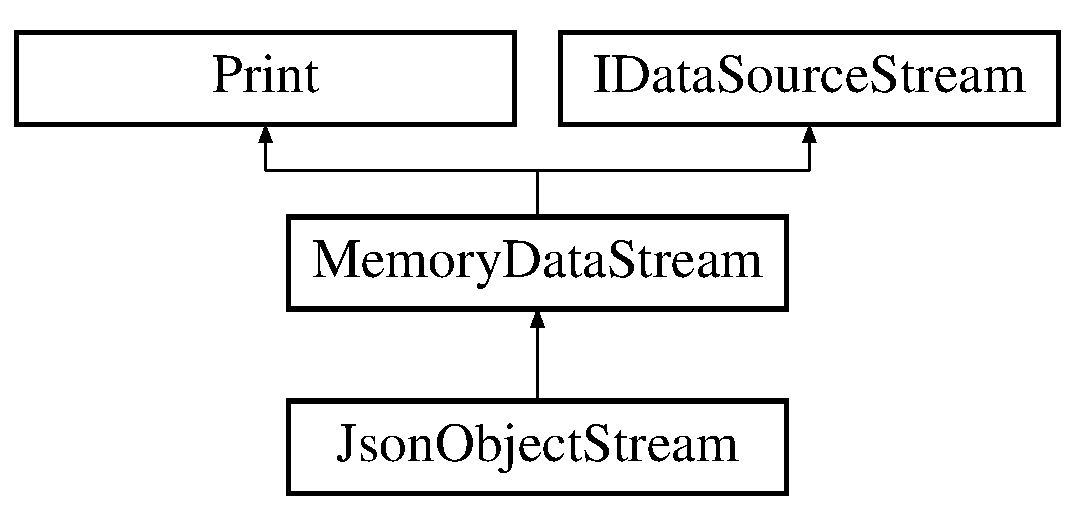
\includegraphics[height=3.000000cm]{class_json_object_stream}
\end{center}
\end{figure}
\subsection*{Public Member Functions}
\begin{DoxyCompactItemize}
\item 
\hypertarget{class_json_object_stream_abe3d3dc8206bb99ff332c25cf0cc0dfd}{}virtual Stream\+Type {\bfseries get\+Stream\+Type} ()\label{class_json_object_stream_abe3d3dc8206bb99ff332c25cf0cc0dfd}

\item 
\hypertarget{class_json_object_stream_a11a57e43ef18ff9937045f25cd74c607}{}\hyperlink{class_arduino_json_1_1_json_object}{Json\+Object} \& {\bfseries get\+Root} ()\label{class_json_object_stream_a11a57e43ef18ff9937045f25cd74c607}

\item 
\hypertarget{class_json_object_stream_ad559ca28b1f7138c8cac4292da1e67bf}{}virtual uint16\+\_\+t {\bfseries get\+Data\+Pointer} (char $\ast$$\ast$data)\label{class_json_object_stream_ad559ca28b1f7138c8cac4292da1e67bf}

\end{DoxyCompactItemize}


The documentation for this class was generated from the following files\+:\begin{DoxyCompactItemize}
\item 
Sming\+Core/Data\+Source\+Stream.\+h\item 
Sming\+Core/Data\+Source\+Stream.\+cpp\end{DoxyCompactItemize}

\hypertarget{struct_arduino_json_1_1_json_pair}{}\section{Arduino\+Json\+:\+:Json\+Pair Struct Reference}
\label{struct_arduino_json_1_1_json_pair}\index{Arduino\+Json\+::\+Json\+Pair@{Arduino\+Json\+::\+Json\+Pair}}
\subsection*{Public Attributes}
\begin{DoxyCompactItemize}
\item 
\hypertarget{struct_arduino_json_1_1_json_pair_adce629ace0a4624d68fc457bb3de3bfa}{}const char $\ast$ {\bfseries key}\label{struct_arduino_json_1_1_json_pair_adce629ace0a4624d68fc457bb3de3bfa}

\item 
\hypertarget{struct_arduino_json_1_1_json_pair_a77395ae9e49e004ef3733fda5a0a4854}{}\hyperlink{class_arduino_json_1_1_json_variant}{Json\+Variant} {\bfseries value}\label{struct_arduino_json_1_1_json_pair_a77395ae9e49e004ef3733fda5a0a4854}

\end{DoxyCompactItemize}


The documentation for this struct was generated from the following file\+:\begin{DoxyCompactItemize}
\item 
Services/\+Arduino\+Json/include/\+Arduino\+Json/Json\+Pair.\+hpp\end{DoxyCompactItemize}

\hypertarget{class_arduino_json_1_1_internals_1_1_json_parser}{}\section{Arduino\+Json\+:\+:Internals\+:\+:Json\+Parser Class Reference}
\label{class_arduino_json_1_1_internals_1_1_json_parser}\index{Arduino\+Json\+::\+Internals\+::\+Json\+Parser@{Arduino\+Json\+::\+Internals\+::\+Json\+Parser}}
\subsection*{Public Member Functions}
\begin{DoxyCompactItemize}
\item 
\hypertarget{class_arduino_json_1_1_internals_1_1_json_parser_a0448df03d89dfcbc3da5475dc32cbd19}{}{\bfseries Json\+Parser} (\hyperlink{class_arduino_json_1_1_json_buffer}{Json\+Buffer} $\ast$buffer, char $\ast$json, uint8\+\_\+t nesting\+Limit)\label{class_arduino_json_1_1_internals_1_1_json_parser_a0448df03d89dfcbc3da5475dc32cbd19}

\item 
\hypertarget{class_arduino_json_1_1_internals_1_1_json_parser_af1a10a294c9fe885205b0819fd92dbaf}{}\hyperlink{class_arduino_json_1_1_json_array}{Json\+Array} \& {\bfseries parse\+Array} ()\label{class_arduino_json_1_1_internals_1_1_json_parser_af1a10a294c9fe885205b0819fd92dbaf}

\item 
\hypertarget{class_arduino_json_1_1_internals_1_1_json_parser_a575bd8cf8b23c8862ee77f0f171bf8fc}{}\hyperlink{class_arduino_json_1_1_json_object}{Json\+Object} \& {\bfseries parse\+Object} ()\label{class_arduino_json_1_1_internals_1_1_json_parser_a575bd8cf8b23c8862ee77f0f171bf8fc}

\end{DoxyCompactItemize}


The documentation for this class was generated from the following files\+:\begin{DoxyCompactItemize}
\item 
Services/\+Arduino\+Json/include/\+Arduino\+Json/\+Internals/Json\+Parser.\+hpp\item 
Services/\+Arduino\+Json/src/\+Internals/Json\+Parser.\+cpp\end{DoxyCompactItemize}

\hypertarget{class_arduino_json_1_1_internals_1_1_json_printable}{}\section{Arduino\+Json\+:\+:Internals\+:\+:Json\+Printable$<$ T $>$ Class Template Reference}
\label{class_arduino_json_1_1_internals_1_1_json_printable}\index{Arduino\+Json\+::\+Internals\+::\+Json\+Printable$<$ T $>$@{Arduino\+Json\+::\+Internals\+::\+Json\+Printable$<$ T $>$}}
\subsection*{Public Member Functions}
\begin{DoxyCompactItemize}
\item 
\hypertarget{class_arduino_json_1_1_internals_1_1_json_printable_a196e6bbbbcc098504cb44b659a6f158b}{}size\+\_\+t {\bfseries print\+To} (Print \&print) const \label{class_arduino_json_1_1_internals_1_1_json_printable_a196e6bbbbcc098504cb44b659a6f158b}

\item 
\hypertarget{class_arduino_json_1_1_internals_1_1_json_printable_a22891b58af25ae55a70743a8c5ea1395}{}size\+\_\+t {\bfseries print\+To} (char $\ast$buffer, size\+\_\+t buffer\+Size) const \label{class_arduino_json_1_1_internals_1_1_json_printable_a22891b58af25ae55a70743a8c5ea1395}

\item 
\hypertarget{class_arduino_json_1_1_internals_1_1_json_printable_af16a5340d0119c7775646a886adc414c}{}size\+\_\+t {\bfseries pretty\+Print\+To} (\hyperlink{class_arduino_json_1_1_internals_1_1_indented_print}{Indented\+Print} \&print) const \label{class_arduino_json_1_1_internals_1_1_json_printable_af16a5340d0119c7775646a886adc414c}

\item 
\hypertarget{class_arduino_json_1_1_internals_1_1_json_printable_a03bcf4647271406978c558ad7d6e2754}{}size\+\_\+t {\bfseries pretty\+Print\+To} (char $\ast$buffer, size\+\_\+t buffer\+Size) const \label{class_arduino_json_1_1_internals_1_1_json_printable_a03bcf4647271406978c558ad7d6e2754}

\item 
\hypertarget{class_arduino_json_1_1_internals_1_1_json_printable_ad9d30b93923cb5b5dbc8f5c9fb4c415f}{}size\+\_\+t {\bfseries pretty\+Print\+To} (Print \&print) const \label{class_arduino_json_1_1_internals_1_1_json_printable_ad9d30b93923cb5b5dbc8f5c9fb4c415f}

\end{DoxyCompactItemize}


The documentation for this class was generated from the following file\+:\begin{DoxyCompactItemize}
\item 
Services/\+Arduino\+Json/include/\+Arduino\+Json/\+Internals/Json\+Printable.\+hpp\end{DoxyCompactItemize}

\hypertarget{class_arduino_json_1_1_json_variant}{}\section{Arduino\+Json\+:\+:Json\+Variant Class Reference}
\label{class_arduino_json_1_1_json_variant}\index{Arduino\+Json\+::\+Json\+Variant@{Arduino\+Json\+::\+Json\+Variant}}
Inheritance diagram for Arduino\+Json\+:\+:Json\+Variant\+:\begin{figure}[H]
\begin{center}
\leavevmode
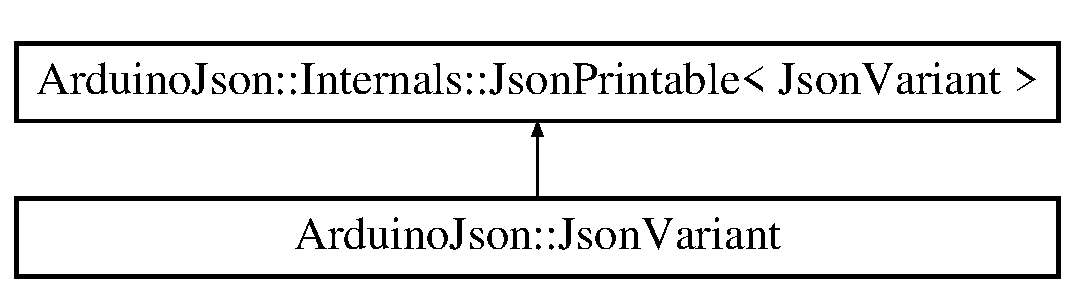
\includegraphics[height=2.000000cm]{class_arduino_json_1_1_json_variant}
\end{center}
\end{figure}
\subsection*{Public Member Functions}
\begin{DoxyCompactItemize}
\item 
\hypertarget{class_arduino_json_1_1_json_variant_ae2c6bb2ba0ae85158bcec704c56ee15d}{}{\footnotesize template$<$typename T $>$ }\\{\bfseries Json\+Variant} (T value)\label{class_arduino_json_1_1_json_variant_ae2c6bb2ba0ae85158bcec704c56ee15d}

\item 
\hypertarget{class_arduino_json_1_1_json_variant_a37973a23ba2d09024b69b77a845822f2}{}bool {\bfseries success} () const \label{class_arduino_json_1_1_json_variant_a37973a23ba2d09024b69b77a845822f2}

\item 
\hypertarget{class_arduino_json_1_1_json_variant_a5ff18fdba8ce245bc2019312e99a04db}{}void {\bfseries set} (bool value)\label{class_arduino_json_1_1_json_variant_a5ff18fdba8ce245bc2019312e99a04db}

\item 
\hypertarget{class_arduino_json_1_1_json_variant_ab7c02236c9bb43628115fa5fcb0cca9c}{}void {\bfseries set} (double value, uint8\+\_\+t decimals=2)\label{class_arduino_json_1_1_json_variant_ab7c02236c9bb43628115fa5fcb0cca9c}

\item 
\hypertarget{class_arduino_json_1_1_json_variant_a329666228b5a5979a2fd33b761379ffe}{}void {\bfseries set} (signed long value)\label{class_arduino_json_1_1_json_variant_a329666228b5a5979a2fd33b761379ffe}

\item 
\hypertarget{class_arduino_json_1_1_json_variant_ab66d2559a08cb01b5d508cacb799e481}{}void {\bfseries set} (signed char value)\label{class_arduino_json_1_1_json_variant_ab66d2559a08cb01b5d508cacb799e481}

\item 
\hypertarget{class_arduino_json_1_1_json_variant_a59c1ea0167c7b365b284b3524fe94556}{}void {\bfseries set} (signed int value)\label{class_arduino_json_1_1_json_variant_a59c1ea0167c7b365b284b3524fe94556}

\item 
\hypertarget{class_arduino_json_1_1_json_variant_a54269623964ff70cb0f4c76b7e93e83e}{}void {\bfseries set} (signed short value)\label{class_arduino_json_1_1_json_variant_a54269623964ff70cb0f4c76b7e93e83e}

\item 
\hypertarget{class_arduino_json_1_1_json_variant_aa1309df7cac01305fb0e53942b0960dc}{}void {\bfseries set} (unsigned char value)\label{class_arduino_json_1_1_json_variant_aa1309df7cac01305fb0e53942b0960dc}

\item 
\hypertarget{class_arduino_json_1_1_json_variant_a435ca24e4efd79d07d32963d78c9ae74}{}void {\bfseries set} (unsigned int value)\label{class_arduino_json_1_1_json_variant_a435ca24e4efd79d07d32963d78c9ae74}

\item 
\hypertarget{class_arduino_json_1_1_json_variant_a2f4919ea494631bd3dd657868c073a86}{}void {\bfseries set} (unsigned long value)\label{class_arduino_json_1_1_json_variant_a2f4919ea494631bd3dd657868c073a86}

\item 
\hypertarget{class_arduino_json_1_1_json_variant_aaa77e8f0510b9368772d93a93908a6e9}{}void {\bfseries set} (unsigned short value)\label{class_arduino_json_1_1_json_variant_aaa77e8f0510b9368772d93a93908a6e9}

\item 
\hypertarget{class_arduino_json_1_1_json_variant_a1c4e58263321e8748ad95b4f6fc06553}{}void {\bfseries set} (const char $\ast$value)\label{class_arduino_json_1_1_json_variant_a1c4e58263321e8748ad95b4f6fc06553}

\item 
\hypertarget{class_arduino_json_1_1_json_variant_a6c6ec86d8b147b508fc2e1be160a24f4}{}void {\bfseries set} (const String \&value)\label{class_arduino_json_1_1_json_variant_a6c6ec86d8b147b508fc2e1be160a24f4}

\item 
\hypertarget{class_arduino_json_1_1_json_variant_aac79b7e447ab28f1ac17a33272381324}{}void {\bfseries set} (\hyperlink{class_arduino_json_1_1_json_array}{Json\+Array} \&array)\label{class_arduino_json_1_1_json_variant_aac79b7e447ab28f1ac17a33272381324}

\item 
\hypertarget{class_arduino_json_1_1_json_variant_aba035c1cde623dc494ca2cf443daf350}{}void {\bfseries set} (\hyperlink{class_arduino_json_1_1_json_object}{Json\+Object} \&object)\label{class_arduino_json_1_1_json_variant_aba035c1cde623dc494ca2cf443daf350}

\item 
\hypertarget{class_arduino_json_1_1_json_variant_ab4ba58898a8ec965c39dc1ebfdb03996}{}{\footnotesize template$<$typename T $>$ }\\\hyperlink{class_arduino_json_1_1_json_variant}{Json\+Variant} \& {\bfseries operator=} (T value)\label{class_arduino_json_1_1_json_variant_ab4ba58898a8ec965c39dc1ebfdb03996}

\item 
\hypertarget{class_arduino_json_1_1_json_variant_a8ccc8b7a50621243692ced64aaf582c0}{}\hyperlink{class_arduino_json_1_1_json_variant}{Json\+Variant} \& {\bfseries operator=} (\hyperlink{class_arduino_json_1_1_json_array}{Json\+Array} \&array)\label{class_arduino_json_1_1_json_variant_a8ccc8b7a50621243692ced64aaf582c0}

\item 
\hypertarget{class_arduino_json_1_1_json_variant_a8f97fd0504955ad46992619b0edaded4}{}\hyperlink{class_arduino_json_1_1_json_variant}{Json\+Variant} \& {\bfseries operator=} (\hyperlink{class_arduino_json_1_1_json_object}{Json\+Object} \&object)\label{class_arduino_json_1_1_json_variant_a8f97fd0504955ad46992619b0edaded4}

\item 
\hypertarget{class_arduino_json_1_1_json_variant_a06fcd2564be88335c9fed444526c3c5d}{}\hyperlink{class_arduino_json_1_1_json_variant}{Json\+Variant} \& {\bfseries operator=} (const String \&value)\label{class_arduino_json_1_1_json_variant_a06fcd2564be88335c9fed444526c3c5d}

\item 
\hypertarget{class_arduino_json_1_1_json_variant_a703111826edb73fad15863bd7b9b4efb}{}{\bfseries operator bool} () const \label{class_arduino_json_1_1_json_variant_a703111826edb73fad15863bd7b9b4efb}

\item 
\hypertarget{class_arduino_json_1_1_json_variant_a38a010a76383519b2cb36461ba0c28a6}{}{\bfseries operator double} () const \label{class_arduino_json_1_1_json_variant_a38a010a76383519b2cb36461ba0c28a6}

\item 
\hypertarget{class_arduino_json_1_1_json_variant_a75b62943a12ed758f0995ec25c3d5a15}{}{\bfseries operator float} () const \label{class_arduino_json_1_1_json_variant_a75b62943a12ed758f0995ec25c3d5a15}

\item 
\hypertarget{class_arduino_json_1_1_json_variant_a3b77aac6ab4f89190b48c07ec4a75ef5}{}{\bfseries operator signed long} () const \label{class_arduino_json_1_1_json_variant_a3b77aac6ab4f89190b48c07ec4a75ef5}

\item 
\hypertarget{class_arduino_json_1_1_json_variant_ac0c7b37437762b343072b30ae34923ee}{}{\bfseries operator signed char} () const \label{class_arduino_json_1_1_json_variant_ac0c7b37437762b343072b30ae34923ee}

\item 
\hypertarget{class_arduino_json_1_1_json_variant_a35fc423863bfa29ea51925bafa0cbd20}{}{\bfseries operator signed int} () const \label{class_arduino_json_1_1_json_variant_a35fc423863bfa29ea51925bafa0cbd20}

\item 
\hypertarget{class_arduino_json_1_1_json_variant_a7a2056611d5e6e3c2b7f79f2cc4aa810}{}{\bfseries operator signed short} () const \label{class_arduino_json_1_1_json_variant_a7a2056611d5e6e3c2b7f79f2cc4aa810}

\item 
\hypertarget{class_arduino_json_1_1_json_variant_a34a17af8366b0b7e766c0e132e7a1ebd}{}{\bfseries operator unsigned char} () const \label{class_arduino_json_1_1_json_variant_a34a17af8366b0b7e766c0e132e7a1ebd}

\item 
\hypertarget{class_arduino_json_1_1_json_variant_a8522c303081b1282d3a202bd31edf083}{}{\bfseries operator unsigned int} () const \label{class_arduino_json_1_1_json_variant_a8522c303081b1282d3a202bd31edf083}

\item 
\hypertarget{class_arduino_json_1_1_json_variant_abd7b351eca553e6800c441d5b352b989}{}{\bfseries operator unsigned long} () const \label{class_arduino_json_1_1_json_variant_abd7b351eca553e6800c441d5b352b989}

\item 
\hypertarget{class_arduino_json_1_1_json_variant_a4a3a52f22499e45b3c3d83776b437b65}{}{\bfseries operator unsigned short} () const \label{class_arduino_json_1_1_json_variant_a4a3a52f22499e45b3c3d83776b437b65}

\item 
\hypertarget{class_arduino_json_1_1_json_variant_ae978efbdaa199407438da92cce6e7baa}{}{\bfseries operator const String $\ast$} () const \label{class_arduino_json_1_1_json_variant_ae978efbdaa199407438da92cce6e7baa}

\item 
\hypertarget{class_arduino_json_1_1_json_variant_aa899c274fa87c548444748b15ae7f81d}{}{\bfseries operator const char $\ast$} () const \label{class_arduino_json_1_1_json_variant_aa899c274fa87c548444748b15ae7f81d}

\item 
\hypertarget{class_arduino_json_1_1_json_variant_aafc77c40a1404c949c68f9976a23b48e}{}const char $\ast$ {\bfseries as\+String} () const \label{class_arduino_json_1_1_json_variant_aafc77c40a1404c949c68f9976a23b48e}

\item 
\hypertarget{class_arduino_json_1_1_json_variant_a062fbaa951b70345de4482de8a18280c}{}String {\bfseries to\+String} () const \label{class_arduino_json_1_1_json_variant_a062fbaa951b70345de4482de8a18280c}

\item 
\hypertarget{class_arduino_json_1_1_json_variant_a7c891c976db35d3d559557b601d7589e}{}{\bfseries operator Json\+Array \&} () const \label{class_arduino_json_1_1_json_variant_a7c891c976db35d3d559557b601d7589e}

\item 
\hypertarget{class_arduino_json_1_1_json_variant_a733686942f0d1142eee67de41c314654}{}\hyperlink{class_arduino_json_1_1_json_array}{Json\+Array} \& {\bfseries as\+Array} () const \label{class_arduino_json_1_1_json_variant_a733686942f0d1142eee67de41c314654}

\item 
\hypertarget{class_arduino_json_1_1_json_variant_a41ee36aff9f45c10da571c7e88f39807}{}{\bfseries operator Json\+Object \&} () const \label{class_arduino_json_1_1_json_variant_a41ee36aff9f45c10da571c7e88f39807}

\item 
\hypertarget{class_arduino_json_1_1_json_variant_a0f564a30c942d14788ee280c4cf685d7}{}\hyperlink{class_arduino_json_1_1_json_object}{Json\+Object} \& {\bfseries as\+Object} () const \label{class_arduino_json_1_1_json_variant_a0f564a30c942d14788ee280c4cf685d7}

\item 
\hypertarget{class_arduino_json_1_1_json_variant_a6a683bd87177bb4fd309581608e19f23}{}{\footnotesize template$<$typename T $>$ }\\T {\bfseries as} () const \label{class_arduino_json_1_1_json_variant_a6a683bd87177bb4fd309581608e19f23}

\item 
\hypertarget{class_arduino_json_1_1_json_variant_add706f7fac7a0a0333b5cc55f5094011}{}{\footnotesize template$<$typename T $>$ }\\bool {\bfseries is} () const \label{class_arduino_json_1_1_json_variant_add706f7fac7a0a0333b5cc55f5094011}

\item 
\hypertarget{class_arduino_json_1_1_json_variant_aa7586c7455210e960a87acba191d69bb}{}void {\bfseries write\+To} (\hyperlink{class_arduino_json_1_1_internals_1_1_json_writer}{Internals\+::\+Json\+Writer} \&writer) const \label{class_arduino_json_1_1_json_variant_aa7586c7455210e960a87acba191d69bb}

\item 
\hypertarget{class_arduino_json_1_1_json_variant_a5f4a989cba96104a21da09fab5e80dc4}{}size\+\_\+t {\bfseries size} () const \label{class_arduino_json_1_1_json_variant_a5f4a989cba96104a21da09fab5e80dc4}

\item 
\hypertarget{class_arduino_json_1_1_json_variant_aaceb78c775794ac2947411ac654945c8}{}\hyperlink{class_arduino_json_1_1_json_variant}{Json\+Variant} \& {\bfseries operator\mbox{[}$\,$\mbox{]}} (int index)\label{class_arduino_json_1_1_json_variant_aaceb78c775794ac2947411ac654945c8}

\item 
\hypertarget{class_arduino_json_1_1_json_variant_a10805433be041a3065e3e2f11d07d82b}{}\hyperlink{class_arduino_json_1_1_json_variant}{Json\+Variant} \& {\bfseries operator\mbox{[}$\,$\mbox{]}} (const char $\ast$key)\label{class_arduino_json_1_1_json_variant_a10805433be041a3065e3e2f11d07d82b}

\item 
\hypertarget{class_arduino_json_1_1_json_variant_a4c7167a72efd02a254688616634ebf55}{}{\footnotesize template$<$$>$ }\\bool {\bfseries is} () const \label{class_arduino_json_1_1_json_variant_a4c7167a72efd02a254688616634ebf55}

\item 
\hypertarget{class_arduino_json_1_1_json_variant_a4c7167a72efd02a254688616634ebf55}{}{\footnotesize template$<$$>$ }\\bool {\bfseries is} () const \label{class_arduino_json_1_1_json_variant_a4c7167a72efd02a254688616634ebf55}

\item 
\hypertarget{class_arduino_json_1_1_json_variant_a4c7167a72efd02a254688616634ebf55}{}{\footnotesize template$<$$>$ }\\bool {\bfseries is} () const \label{class_arduino_json_1_1_json_variant_a4c7167a72efd02a254688616634ebf55}

\item 
\hypertarget{class_arduino_json_1_1_json_variant_a4c7167a72efd02a254688616634ebf55}{}{\footnotesize template$<$$>$ }\\bool {\bfseries is} () const \label{class_arduino_json_1_1_json_variant_a4c7167a72efd02a254688616634ebf55}

\item 
\hypertarget{class_arduino_json_1_1_json_variant_a4c7167a72efd02a254688616634ebf55}{}{\footnotesize template$<$$>$ }\\bool {\bfseries is} () const \label{class_arduino_json_1_1_json_variant_a4c7167a72efd02a254688616634ebf55}

\item 
\hypertarget{class_arduino_json_1_1_json_variant_a4c7167a72efd02a254688616634ebf55}{}{\footnotesize template$<$$>$ }\\bool {\bfseries is} () const \label{class_arduino_json_1_1_json_variant_a4c7167a72efd02a254688616634ebf55}

\item 
\hypertarget{class_arduino_json_1_1_json_variant_a4c7167a72efd02a254688616634ebf55}{}{\footnotesize template$<$$>$ }\\bool {\bfseries is} () const \label{class_arduino_json_1_1_json_variant_a4c7167a72efd02a254688616634ebf55}

\item 
\hypertarget{class_arduino_json_1_1_json_variant_a4c7167a72efd02a254688616634ebf55}{}{\footnotesize template$<$$>$ }\\bool {\bfseries is} () const \label{class_arduino_json_1_1_json_variant_a4c7167a72efd02a254688616634ebf55}

\item 
\hypertarget{class_arduino_json_1_1_json_variant_a4c7167a72efd02a254688616634ebf55}{}{\footnotesize template$<$$>$ }\\bool {\bfseries is} () const \label{class_arduino_json_1_1_json_variant_a4c7167a72efd02a254688616634ebf55}

\end{DoxyCompactItemize}
\subsection*{Static Public Member Functions}
\begin{DoxyCompactItemize}
\item 
\hypertarget{class_arduino_json_1_1_json_variant_a92704bcc018c798575a3432fd3cfb1bb}{}static \hyperlink{class_arduino_json_1_1_json_variant}{Json\+Variant} \& {\bfseries invalid} ()\label{class_arduino_json_1_1_json_variant_a92704bcc018c798575a3432fd3cfb1bb}

\end{DoxyCompactItemize}


The documentation for this class was generated from the following files\+:\begin{DoxyCompactItemize}
\item 
Services/\+Arduino\+Json/include/\+Arduino\+Json/Json\+Variant.\+hpp\item 
Services/\+Arduino\+Json/src/Json\+Variant.\+cpp\end{DoxyCompactItemize}

\hypertarget{union_arduino_json_1_1_internals_1_1_json_variant_content}{}\section{Arduino\+Json\+:\+:Internals\+:\+:Json\+Variant\+Content Union Reference}
\label{union_arduino_json_1_1_internals_1_1_json_variant_content}\index{Arduino\+Json\+::\+Internals\+::\+Json\+Variant\+Content@{Arduino\+Json\+::\+Internals\+::\+Json\+Variant\+Content}}
\subsection*{Public Attributes}
\begin{DoxyCompactItemize}
\item 
\hypertarget{union_arduino_json_1_1_internals_1_1_json_variant_content_a972d56c674b5e090505f56f4fa5b95fd}{}bool {\bfseries as\+Boolean}\label{union_arduino_json_1_1_internals_1_1_json_variant_content_a972d56c674b5e090505f56f4fa5b95fd}

\item 
\hypertarget{union_arduino_json_1_1_internals_1_1_json_variant_content_aafa12c0f2ed15255e99d3f2838c19fb8}{}double {\bfseries as\+Double}\label{union_arduino_json_1_1_internals_1_1_json_variant_content_aafa12c0f2ed15255e99d3f2838c19fb8}

\item 
\hypertarget{union_arduino_json_1_1_internals_1_1_json_variant_content_ac0f5263826960638b68e93092e8c3440}{}long {\bfseries as\+Long}\label{union_arduino_json_1_1_internals_1_1_json_variant_content_ac0f5263826960638b68e93092e8c3440}

\item 
\hypertarget{union_arduino_json_1_1_internals_1_1_json_variant_content_ab400fe863020ab5c4cc5f0e460dfcdfe}{}const char $\ast$ {\bfseries as\+String}\label{union_arduino_json_1_1_internals_1_1_json_variant_content_ab400fe863020ab5c4cc5f0e460dfcdfe}

\item 
\hypertarget{union_arduino_json_1_1_internals_1_1_json_variant_content_a0f2dd2b955f2eabdee4da7dc8127e328}{}\hyperlink{class_arduino_json_1_1_json_array}{Json\+Array} $\ast$ {\bfseries as\+Array}\label{union_arduino_json_1_1_internals_1_1_json_variant_content_a0f2dd2b955f2eabdee4da7dc8127e328}

\item 
\hypertarget{union_arduino_json_1_1_internals_1_1_json_variant_content_ae07d27d7bde99a3305e9f7218f74111a}{}\hyperlink{class_arduino_json_1_1_json_object}{Json\+Object} $\ast$ {\bfseries as\+Object}\label{union_arduino_json_1_1_internals_1_1_json_variant_content_ae07d27d7bde99a3305e9f7218f74111a}

\item 
\hypertarget{union_arduino_json_1_1_internals_1_1_json_variant_content_a636471ba024df5aaff87eb05c2c4aa3c}{}const String $\ast$ {\bfseries as\+C\+String}\label{union_arduino_json_1_1_internals_1_1_json_variant_content_a636471ba024df5aaff87eb05c2c4aa3c}

\end{DoxyCompactItemize}


The documentation for this union was generated from the following file\+:\begin{DoxyCompactItemize}
\item 
Services/\+Arduino\+Json/include/\+Arduino\+Json/\+Internals/Json\+Variant\+Content.\+hpp\end{DoxyCompactItemize}

\hypertarget{class_arduino_json_1_1_internals_1_1_json_writer}{}\section{Arduino\+Json\+:\+:Internals\+:\+:Json\+Writer Class Reference}
\label{class_arduino_json_1_1_internals_1_1_json_writer}\index{Arduino\+Json\+::\+Internals\+::\+Json\+Writer@{Arduino\+Json\+::\+Internals\+::\+Json\+Writer}}
\subsection*{Public Member Functions}
\begin{DoxyCompactItemize}
\item 
\hypertarget{class_arduino_json_1_1_internals_1_1_json_writer_a29549cb139e22532c8dcd7fdd4570955}{}{\bfseries Json\+Writer} (Print \&sink)\label{class_arduino_json_1_1_internals_1_1_json_writer_a29549cb139e22532c8dcd7fdd4570955}

\item 
\hypertarget{class_arduino_json_1_1_internals_1_1_json_writer_a491d15e06706647bf148865af4db6498}{}size\+\_\+t {\bfseries bytes\+Written} ()\label{class_arduino_json_1_1_internals_1_1_json_writer_a491d15e06706647bf148865af4db6498}

\item 
\hypertarget{class_arduino_json_1_1_internals_1_1_json_writer_a368c20f3443b2c10b23c9ea18c6ef466}{}void {\bfseries begin\+Array} ()\label{class_arduino_json_1_1_internals_1_1_json_writer_a368c20f3443b2c10b23c9ea18c6ef466}

\item 
\hypertarget{class_arduino_json_1_1_internals_1_1_json_writer_ad4a25a30f3dc8a6aac5c62355c3fddd8}{}void {\bfseries end\+Array} ()\label{class_arduino_json_1_1_internals_1_1_json_writer_ad4a25a30f3dc8a6aac5c62355c3fddd8}

\item 
\hypertarget{class_arduino_json_1_1_internals_1_1_json_writer_a8a907d2782560df604af5c16ef03c744}{}void {\bfseries begin\+Object} ()\label{class_arduino_json_1_1_internals_1_1_json_writer_a8a907d2782560df604af5c16ef03c744}

\item 
\hypertarget{class_arduino_json_1_1_internals_1_1_json_writer_af223bff28545a6bc589857ecb541e049}{}void {\bfseries end\+Object} ()\label{class_arduino_json_1_1_internals_1_1_json_writer_af223bff28545a6bc589857ecb541e049}

\item 
\hypertarget{class_arduino_json_1_1_internals_1_1_json_writer_a909e8a284ae245699c8779299248f79c}{}void {\bfseries write\+Colon} ()\label{class_arduino_json_1_1_internals_1_1_json_writer_a909e8a284ae245699c8779299248f79c}

\item 
\hypertarget{class_arduino_json_1_1_internals_1_1_json_writer_a17d14e25639f61f9b8114dae8c5c9ab8}{}void {\bfseries write\+Comma} ()\label{class_arduino_json_1_1_internals_1_1_json_writer_a17d14e25639f61f9b8114dae8c5c9ab8}

\item 
\hypertarget{class_arduino_json_1_1_internals_1_1_json_writer_a67e8a339758de2e46a14bf6e00b21a73}{}void {\bfseries write\+String} (const char $\ast$value)\label{class_arduino_json_1_1_internals_1_1_json_writer_a67e8a339758de2e46a14bf6e00b21a73}

\item 
\hypertarget{class_arduino_json_1_1_internals_1_1_json_writer_aeb182995643bb087558316df87c24884}{}void {\bfseries write\+Long} (long value)\label{class_arduino_json_1_1_internals_1_1_json_writer_aeb182995643bb087558316df87c24884}

\item 
\hypertarget{class_arduino_json_1_1_internals_1_1_json_writer_a25cbf2177aaedf05d046194ab812bc05}{}void {\bfseries write\+Boolean} (bool value)\label{class_arduino_json_1_1_internals_1_1_json_writer_a25cbf2177aaedf05d046194ab812bc05}

\item 
\hypertarget{class_arduino_json_1_1_internals_1_1_json_writer_aecefdc2de9bfc49c960281c1c1b76121}{}void {\bfseries write\+Double} (double value, uint8\+\_\+t decimals)\label{class_arduino_json_1_1_internals_1_1_json_writer_aecefdc2de9bfc49c960281c1c1b76121}

\end{DoxyCompactItemize}
\subsection*{Protected Member Functions}
\begin{DoxyCompactItemize}
\item 
\hypertarget{class_arduino_json_1_1_internals_1_1_json_writer_a83b6cb4e48bc74e6dc8db25df0e393c0}{}void {\bfseries write} (char c)\label{class_arduino_json_1_1_internals_1_1_json_writer_a83b6cb4e48bc74e6dc8db25df0e393c0}

\item 
\hypertarget{class_arduino_json_1_1_internals_1_1_json_writer_aa2757d66f17cddb66f27447c5c283fb3}{}void {\bfseries write} (const char $\ast$s)\label{class_arduino_json_1_1_internals_1_1_json_writer_aa2757d66f17cddb66f27447c5c283fb3}

\end{DoxyCompactItemize}
\subsection*{Protected Attributes}
\begin{DoxyCompactItemize}
\item 
\hypertarget{class_arduino_json_1_1_internals_1_1_json_writer_a61c8af5b5665d3836dedf28a41127f56}{}Print \& {\bfseries \+\_\+sink}\label{class_arduino_json_1_1_internals_1_1_json_writer_a61c8af5b5665d3836dedf28a41127f56}

\item 
\hypertarget{class_arduino_json_1_1_internals_1_1_json_writer_a513a8602e4a333abf9c70601ff0b1c67}{}size\+\_\+t {\bfseries \+\_\+length}\label{class_arduino_json_1_1_internals_1_1_json_writer_a513a8602e4a333abf9c70601ff0b1c67}

\end{DoxyCompactItemize}


The documentation for this class was generated from the following file\+:\begin{DoxyCompactItemize}
\item 
Services/\+Arduino\+Json/include/\+Arduino\+Json/\+Internals/Json\+Writer.\+hpp\end{DoxyCompactItemize}

\hypertarget{class_l_c_d}{}\section{L\+C\+D Class Reference}
\label{class_l_c_d}\index{L\+C\+D@{L\+C\+D}}
Inheritance diagram for L\+C\+D\+:\begin{figure}[H]
\begin{center}
\leavevmode
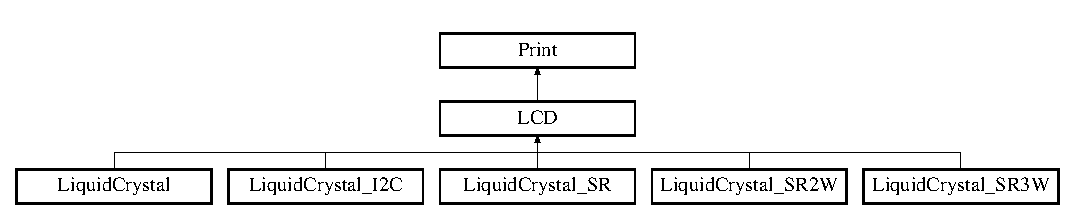
\includegraphics[height=2.507463cm]{class_l_c_d}
\end{center}
\end{figure}
\subsection*{Public Member Functions}
\begin{DoxyCompactItemize}
\item 
\hyperlink{class_l_c_d_a00bb2db1390721abc7b24ac4b8c276c8}{L\+C\+D} ()
\item 
virtual void \hyperlink{class_l_c_d_a3f587d1cbb2d59765ef60a5216b56fea}{begin} (uint8\+\_\+t cols, uint8\+\_\+t rows, uint8\+\_\+t charsize=L\+C\+D\+\_\+5x8\+D\+O\+T\+S)
\item 
void \hyperlink{class_l_c_d_afa699e0beeeee03cce8cef87eba81c4a}{clear} ()
\item 
void \hyperlink{class_l_c_d_aee45ad37f09312f5d9982257e2d37e68}{home} ()
\item 
void \hyperlink{class_l_c_d_af3974da6d988ba2d21c25135ada12108}{no\+Display} ()
\item 
void \hyperlink{class_l_c_d_a5b07cf05e8e5e7c53654f5ca0cf58b89}{display} ()
\item 
void \hyperlink{class_l_c_d_a3b755c4b397b5985752be8c30ee1a9b5}{no\+Blink} ()
\item 
void \hyperlink{class_l_c_d_a878b36878fa8287093964eba83aace77}{blink} ()
\item 
void \hyperlink{class_l_c_d_aec8ffaa1e69c7a6e13ac0cfbc29151d9}{no\+Cursor} ()
\item 
void \hyperlink{class_l_c_d_a194814f64dfa50a90e07e0fe0d361620}{cursor} ()
\item 
void \hyperlink{class_l_c_d_a6f3a503055b3b8dcf0f61b2633c584f7}{scroll\+Display\+Left} ()
\item 
void \hyperlink{class_l_c_d_abfc44b294772f09020bfa32af8a79571}{scroll\+Display\+Right} ()
\item 
void \hyperlink{class_l_c_d_a238e9f6476dc7df64af04eb6c87f6ac7}{left\+To\+Right} ()
\item 
void \hyperlink{class_l_c_d_ac014830eadc26bfd86308ea8734f4428}{right\+To\+Left} ()
\item 
void \hyperlink{class_l_c_d_aad2abc99d1aca5403873579d9d72c2d4}{move\+Cursor\+Left} ()
\item 
void \hyperlink{class_l_c_d_a09eec0c712e54b066f5894635c1fe75c}{move\+Cursor\+Right} ()
\item 
void \hyperlink{class_l_c_d_abb3ed88d530f6283e6159b4973e7da9e}{autoscroll} ()
\item 
void \hyperlink{class_l_c_d_a96035dde40efbf73390e00b5beb00231}{no\+Autoscroll} ()
\item 
void \hyperlink{class_l_c_d_a91cba8f93c692abcddf8bc3de58d2d3a}{create\+Char} (uint8\+\_\+t location, uint8\+\_\+t charmap\mbox{[}$\,$\mbox{]})
\item 
void \hyperlink{class_l_c_d_a48220450fd152b25994eb7d0ba340e8d}{set\+Cursor} (uint8\+\_\+t col, uint8\+\_\+t row)
\item 
void \hyperlink{class_l_c_d_aba8867fe2210cbfa8db869208709be10}{backlight} (void)
\item 
void \hyperlink{class_l_c_d_a2a331b4e142734411b2f1cfaffe7a488}{no\+Backlight} (void)
\item 
void \hyperlink{class_l_c_d_a718da3a638deb59bd1c7a5222a52d98a}{on} (void)
\item 
void \hyperlink{class_l_c_d_a191639be183be1476c9bfe6d455d23b2}{off} (void)
\item 
virtual void \hyperlink{class_l_c_d_a53f4ee9b39d9ab3d7ae4d9f8dedca3bc}{set\+Backlight\+Pin} (uint8\+\_\+t value, t\+\_\+backligh\+Pol pol)
\item 
virtual void \hyperlink{class_l_c_d_a3305570d7b37eb93f2cf840263c15828}{set\+Backlight} (uint8\+\_\+t value)
\item 
virtual void \hyperlink{class_l_c_d_a2d89cc2e62f72afb5f15a7fd812900e3}{write} (uint8\+\_\+t value)
\end{DoxyCompactItemize}
\subsection*{Protected Attributes}
\begin{DoxyCompactItemize}
\item 
\hypertarget{class_l_c_d_aef093ba3f8e1016267b40ac235a0fa0f}{}uint8\+\_\+t {\bfseries \+\_\+displayfunction}\label{class_l_c_d_aef093ba3f8e1016267b40ac235a0fa0f}

\item 
\hypertarget{class_l_c_d_ae47a0e2eff74431a39774b788d5761f4}{}uint8\+\_\+t {\bfseries \+\_\+displaycontrol}\label{class_l_c_d_ae47a0e2eff74431a39774b788d5761f4}

\item 
\hypertarget{class_l_c_d_a726b9a68d091dd8683a18e83f3a8fd3c}{}uint8\+\_\+t {\bfseries \+\_\+displaymode}\label{class_l_c_d_a726b9a68d091dd8683a18e83f3a8fd3c}

\item 
\hypertarget{class_l_c_d_ac1374911fb145fea430c21092ada0c06}{}uint8\+\_\+t {\bfseries \+\_\+numlines}\label{class_l_c_d_ac1374911fb145fea430c21092ada0c06}

\item 
\hypertarget{class_l_c_d_a88b16ea0e5c7d1cabc5007d48bcbd2b0}{}uint8\+\_\+t {\bfseries \+\_\+cols}\label{class_l_c_d_a88b16ea0e5c7d1cabc5007d48bcbd2b0}

\item 
\hypertarget{class_l_c_d_a990338759d2abe10b0fb1743b7789566}{}t\+\_\+backligh\+Pol {\bfseries \+\_\+polarity}\label{class_l_c_d_a990338759d2abe10b0fb1743b7789566}

\end{DoxyCompactItemize}


\subsection{Constructor \& Destructor Documentation}
\hypertarget{class_l_c_d_a00bb2db1390721abc7b24ac4b8c276c8}{}\index{L\+C\+D@{L\+C\+D}!L\+C\+D@{L\+C\+D}}
\index{L\+C\+D@{L\+C\+D}!L\+C\+D@{L\+C\+D}}
\subsubsection[{L\+C\+D}]{\setlength{\rightskip}{0pt plus 5cm}L\+C\+D\+::\+L\+C\+D (
\begin{DoxyParamCaption}
{}
\end{DoxyParamCaption}
)}\label{class_l_c_d_a00bb2db1390721abc7b24ac4b8c276c8}
\hyperlink{class_liquid_crystal}{Liquid\+Crystal} abstract constructor.  \hyperlink{class_liquid_crystal}{Liquid\+Crystal} class abstract constructor needed to create the base abstract class. 

\subsection{Member Function Documentation}
\hypertarget{class_l_c_d_abb3ed88d530f6283e6159b4973e7da9e}{}\index{L\+C\+D@{L\+C\+D}!autoscroll@{autoscroll}}
\index{autoscroll@{autoscroll}!L\+C\+D@{L\+C\+D}}
\subsubsection[{autoscroll}]{\setlength{\rightskip}{0pt plus 5cm}void L\+C\+D\+::autoscroll (
\begin{DoxyParamCaption}
\item[{void}]{}
\end{DoxyParamCaption}
)}\label{class_l_c_d_abb3ed88d530f6283e6159b4973e7da9e}
Turns on automatic scrolling of the \hyperlink{class_l_c_d}{L\+C\+D}.  Turns on automatic scrolling of the \hyperlink{class_l_c_d}{L\+C\+D}. This causes each character output to the display to push previous characters over by one space. If the current text direction is left-\/to-\/right (the default), the display scrolls to the left; if the current direction is right-\/to-\/left, the display scrolls to the right. This has the effect of outputting each new character to the same location on the \hyperlink{class_l_c_d}{L\+C\+D}.


\begin{DoxyParams}{Parameters}
{\em none} & \\
\hline
\end{DoxyParams}
\hypertarget{class_l_c_d_aba8867fe2210cbfa8db869208709be10}{}\index{L\+C\+D@{L\+C\+D}!backlight@{backlight}}
\index{backlight@{backlight}!L\+C\+D@{L\+C\+D}}
\subsubsection[{backlight}]{\setlength{\rightskip}{0pt plus 5cm}void L\+C\+D\+::backlight (
\begin{DoxyParamCaption}
\item[{void}]{}
\end{DoxyParamCaption}
)}\label{class_l_c_d_aba8867fe2210cbfa8db869208709be10}
Switch-\/on the \hyperlink{class_l_c_d}{L\+C\+D} backlight.  Switch-\/on the \hyperlink{class_l_c_d}{L\+C\+D} backlight. The set\+Backlight\+Pin has to be called before setting the backlight for this method to work. \begin{DoxySeeAlso}{See also}
\hyperlink{class_l_c_d_a53f4ee9b39d9ab3d7ae4d9f8dedca3bc}{set\+Backlight\+Pin}. 
\end{DoxySeeAlso}
\hypertarget{class_l_c_d_a3f587d1cbb2d59765ef60a5216b56fea}{}\index{L\+C\+D@{L\+C\+D}!begin@{begin}}
\index{begin@{begin}!L\+C\+D@{L\+C\+D}}
\subsubsection[{begin}]{\setlength{\rightskip}{0pt plus 5cm}void L\+C\+D\+::begin (
\begin{DoxyParamCaption}
\item[{uint8\+\_\+t}]{cols, }
\item[{uint8\+\_\+t}]{rows, }
\item[{uint8\+\_\+t}]{charsize = {\ttfamily LCD\+\_\+5x8DOTS}}
\end{DoxyParamCaption}
)\hspace{0.3cm}{\ttfamily [virtual]}}\label{class_l_c_d_a3f587d1cbb2d59765ef60a5216b56fea}
\hyperlink{class_l_c_d}{L\+C\+D} initialization.  Initializes the \hyperlink{class_l_c_d}{L\+C\+D} to a given size (col, row). This methods initializes the \hyperlink{class_l_c_d}{L\+C\+D}, therefore, it M\+U\+S\+T be called prior to using any other method from this class.

This method is abstract, a base implementation is available common to all \hyperlink{class_l_c_d}{L\+C\+D} drivers. Should it not be compatible with some other \hyperlink{class_l_c_d}{L\+C\+D} driver, a derived implementation should be done on the driver specif class.


\begin{DoxyParams}{Parameters}
{\em cols\mbox{[}in\mbox{]}} & the number of columns that the display has \\
\hline
{\em rows\mbox{[}in\mbox{]}} & the number of rows that the display has \\
\hline
{\em charsize\mbox{[}in\mbox{]}} & character size, default==L\+C\+D\+\_\+5x8\+D\+O\+T\+S \\
\hline
\end{DoxyParams}


Reimplemented in \hyperlink{class_liquid_crystal___i2_c_aeee2ada537f0cfbfda8613324b57c4a6}{Liquid\+Crystal\+\_\+\+I2\+C}.

\hypertarget{class_l_c_d_a878b36878fa8287093964eba83aace77}{}\index{L\+C\+D@{L\+C\+D}!blink@{blink}}
\index{blink@{blink}!L\+C\+D@{L\+C\+D}}
\subsubsection[{blink}]{\setlength{\rightskip}{0pt plus 5cm}void L\+C\+D\+::blink (
\begin{DoxyParamCaption}
{}
\end{DoxyParamCaption}
)}\label{class_l_c_d_a878b36878fa8287093964eba83aace77}
\hyperlink{class_display}{Display} the cursor of the \hyperlink{class_l_c_d}{L\+C\+D}.  \hyperlink{class_display}{Display} the blinking \hyperlink{class_l_c_d}{L\+C\+D} cursor. If used in combination with the \hyperlink{class_l_c_d_a194814f64dfa50a90e07e0fe0d361620}{cursor()} function, the result will depend on the particular display.


\begin{DoxyParams}{Parameters}
{\em none} & \\
\hline
\end{DoxyParams}
\hypertarget{class_l_c_d_afa699e0beeeee03cce8cef87eba81c4a}{}\index{L\+C\+D@{L\+C\+D}!clear@{clear}}
\index{clear@{clear}!L\+C\+D@{L\+C\+D}}
\subsubsection[{clear}]{\setlength{\rightskip}{0pt plus 5cm}void L\+C\+D\+::clear (
\begin{DoxyParamCaption}
{}
\end{DoxyParamCaption}
)}\label{class_l_c_d_afa699e0beeeee03cce8cef87eba81c4a}
Clears the \hyperlink{class_l_c_d}{L\+C\+D}.  Clears the \hyperlink{class_l_c_d}{L\+C\+D} screen and positions the cursor in the upper-\/left corner.

This operation is time consuming for the \hyperlink{class_l_c_d}{L\+C\+D}.


\begin{DoxyParams}{Parameters}
{\em none} & \\
\hline
\end{DoxyParams}
\hypertarget{class_l_c_d_a91cba8f93c692abcddf8bc3de58d2d3a}{}\index{L\+C\+D@{L\+C\+D}!create\+Char@{create\+Char}}
\index{create\+Char@{create\+Char}!L\+C\+D@{L\+C\+D}}
\subsubsection[{create\+Char}]{\setlength{\rightskip}{0pt plus 5cm}void L\+C\+D\+::create\+Char (
\begin{DoxyParamCaption}
\item[{uint8\+\_\+t}]{location, }
\item[{uint8\+\_\+t}]{charmap\mbox{[}$\,$\mbox{]}}
\end{DoxyParamCaption}
)}\label{class_l_c_d_a91cba8f93c692abcddf8bc3de58d2d3a}
Creates a custom character for use on the \hyperlink{class_l_c_d}{L\+C\+D}.  Create a custom character (glyph) for use on the \hyperlink{class_l_c_d}{L\+C\+D}. Most chipsets only support up to eight characters of 5x8 pixels. Therefore, this methods has been limited to locations (numbered 0 to 7).

The appearance of each custom character is specified by an array of eight bytes, one for each row. The five least significant bits of each byte determine the pixels in that row. To display a custom character on screen, \hyperlink{class_l_c_d_a2d89cc2e62f72afb5f15a7fd812900e3}{write()}/print() its number, i.\+e. lcd.\+print (char(x)); // Where x is 0..7.


\begin{DoxyParams}{Parameters}
{\em location\mbox{[}in\mbox{]}} & \hyperlink{class_l_c_d}{L\+C\+D} memory location of the character to create (0 to 7) \\
\hline
{\em charmap\mbox{[}in\mbox{]}} & the bitmap array representing each row of the character. \\
\hline
\end{DoxyParams}
\hypertarget{class_l_c_d_a194814f64dfa50a90e07e0fe0d361620}{}\index{L\+C\+D@{L\+C\+D}!cursor@{cursor}}
\index{cursor@{cursor}!L\+C\+D@{L\+C\+D}}
\subsubsection[{cursor}]{\setlength{\rightskip}{0pt plus 5cm}void L\+C\+D\+::cursor (
\begin{DoxyParamCaption}
{}
\end{DoxyParamCaption}
)}\label{class_l_c_d_a194814f64dfa50a90e07e0fe0d361620}
\hyperlink{class_display}{Display} the \hyperlink{class_l_c_d}{L\+C\+D} cursor.  \hyperlink{class_display}{Display} the \hyperlink{class_l_c_d}{L\+C\+D} cursor\+: an underscore (line) at the location where the next character will be written.


\begin{DoxyParams}{Parameters}
{\em none} & \\
\hline
\end{DoxyParams}
\hypertarget{class_l_c_d_a5b07cf05e8e5e7c53654f5ca0cf58b89}{}\index{L\+C\+D@{L\+C\+D}!display@{display}}
\index{display@{display}!L\+C\+D@{L\+C\+D}}
\subsubsection[{display}]{\setlength{\rightskip}{0pt plus 5cm}void L\+C\+D\+::display (
\begin{DoxyParamCaption}
\item[{void}]{}
\end{DoxyParamCaption}
)}\label{class_l_c_d_a5b07cf05e8e5e7c53654f5ca0cf58b89}
Turns on the \hyperlink{class_l_c_d}{L\+C\+D} display.  Turns on the \hyperlink{class_l_c_d}{L\+C\+D} display, after it\textquotesingle{}s been turned off with \hyperlink{class_l_c_d_af3974da6d988ba2d21c25135ada12108}{no\+Display()}. This will restore the text (and cursor location) that was on the display prior to calling \hyperlink{class_l_c_d_af3974da6d988ba2d21c25135ada12108}{no\+Display()}.


\begin{DoxyParams}{Parameters}
{\em none} & \\
\hline
\end{DoxyParams}
\hypertarget{class_l_c_d_aee45ad37f09312f5d9982257e2d37e68}{}\index{L\+C\+D@{L\+C\+D}!home@{home}}
\index{home@{home}!L\+C\+D@{L\+C\+D}}
\subsubsection[{home}]{\setlength{\rightskip}{0pt plus 5cm}void L\+C\+D\+::home (
\begin{DoxyParamCaption}
{}
\end{DoxyParamCaption}
)}\label{class_l_c_d_aee45ad37f09312f5d9982257e2d37e68}
Sets the cursor to the upper-\/left corner.  Positions the cursor in the upper-\/left of the \hyperlink{class_l_c_d}{L\+C\+D}. That is, use that location in outputting subsequent text to the display. To also clear the display, use the \hyperlink{class_l_c_d_afa699e0beeeee03cce8cef87eba81c4a}{clear()} function instead.

This operation is time consuming for the \hyperlink{class_l_c_d}{L\+C\+D}.


\begin{DoxyParams}{Parameters}
{\em none} & \\
\hline
\end{DoxyParams}
\hypertarget{class_l_c_d_a238e9f6476dc7df64af04eb6c87f6ac7}{}\index{L\+C\+D@{L\+C\+D}!left\+To\+Right@{left\+To\+Right}}
\index{left\+To\+Right@{left\+To\+Right}!L\+C\+D@{L\+C\+D}}
\subsubsection[{left\+To\+Right}]{\setlength{\rightskip}{0pt plus 5cm}void L\+C\+D\+::left\+To\+Right (
\begin{DoxyParamCaption}
\item[{void}]{}
\end{DoxyParamCaption}
)}\label{class_l_c_d_a238e9f6476dc7df64af04eb6c87f6ac7}
Set the direction for text written to the \hyperlink{class_l_c_d}{L\+C\+D} to left-\/to-\/right.  Set the direction for text written to the \hyperlink{class_l_c_d}{L\+C\+D} to left-\/to-\/right. All subsequent characters written to the display will go from left to right, but does not affect previously-\/output text.

This is the default configuration.


\begin{DoxyParams}{Parameters}
{\em none} & \\
\hline
\end{DoxyParams}
\hypertarget{class_l_c_d_aad2abc99d1aca5403873579d9d72c2d4}{}\index{L\+C\+D@{L\+C\+D}!move\+Cursor\+Left@{move\+Cursor\+Left}}
\index{move\+Cursor\+Left@{move\+Cursor\+Left}!L\+C\+D@{L\+C\+D}}
\subsubsection[{move\+Cursor\+Left}]{\setlength{\rightskip}{0pt plus 5cm}void L\+C\+D\+::move\+Cursor\+Left (
\begin{DoxyParamCaption}
\item[{void}]{}
\end{DoxyParamCaption}
)}\label{class_l_c_d_aad2abc99d1aca5403873579d9d72c2d4}
Moves the cursor one space to the left.  
\begin{DoxyParams}{Parameters}
{\em none} & \\
\hline
\end{DoxyParams}
\hypertarget{class_l_c_d_a09eec0c712e54b066f5894635c1fe75c}{}\index{L\+C\+D@{L\+C\+D}!move\+Cursor\+Right@{move\+Cursor\+Right}}
\index{move\+Cursor\+Right@{move\+Cursor\+Right}!L\+C\+D@{L\+C\+D}}
\subsubsection[{move\+Cursor\+Right}]{\setlength{\rightskip}{0pt plus 5cm}void L\+C\+D\+::move\+Cursor\+Right (
\begin{DoxyParamCaption}
\item[{void}]{}
\end{DoxyParamCaption}
)}\label{class_l_c_d_a09eec0c712e54b066f5894635c1fe75c}
Moves the cursor one space to the right.


\begin{DoxyParams}{Parameters}
{\em none} & \\
\hline
\end{DoxyParams}
\hypertarget{class_l_c_d_a96035dde40efbf73390e00b5beb00231}{}\index{L\+C\+D@{L\+C\+D}!no\+Autoscroll@{no\+Autoscroll}}
\index{no\+Autoscroll@{no\+Autoscroll}!L\+C\+D@{L\+C\+D}}
\subsubsection[{no\+Autoscroll}]{\setlength{\rightskip}{0pt plus 5cm}void L\+C\+D\+::no\+Autoscroll (
\begin{DoxyParamCaption}
\item[{void}]{}
\end{DoxyParamCaption}
)}\label{class_l_c_d_a96035dde40efbf73390e00b5beb00231}
Turns off automatic scrolling of the \hyperlink{class_l_c_d}{L\+C\+D}.  Turns off automatic scrolling of the \hyperlink{class_l_c_d}{L\+C\+D}, this is the default configuration of the \hyperlink{class_l_c_d}{L\+C\+D}.


\begin{DoxyParams}{Parameters}
{\em none} & \\
\hline
\end{DoxyParams}
\hypertarget{class_l_c_d_a2a331b4e142734411b2f1cfaffe7a488}{}\index{L\+C\+D@{L\+C\+D}!no\+Backlight@{no\+Backlight}}
\index{no\+Backlight@{no\+Backlight}!L\+C\+D@{L\+C\+D}}
\subsubsection[{no\+Backlight}]{\setlength{\rightskip}{0pt plus 5cm}void L\+C\+D\+::no\+Backlight (
\begin{DoxyParamCaption}
\item[{void}]{}
\end{DoxyParamCaption}
)}\label{class_l_c_d_a2a331b4e142734411b2f1cfaffe7a488}
Switch-\/off the \hyperlink{class_l_c_d}{L\+C\+D} backlight.  Switch-\/off the \hyperlink{class_l_c_d}{L\+C\+D} backlight. The set\+Backlight\+Pin has to be called before setting the backlight for this method to work. \begin{DoxySeeAlso}{See also}
\hyperlink{class_l_c_d_a53f4ee9b39d9ab3d7ae4d9f8dedca3bc}{set\+Backlight\+Pin}. 
\end{DoxySeeAlso}
\hypertarget{class_l_c_d_a3b755c4b397b5985752be8c30ee1a9b5}{}\index{L\+C\+D@{L\+C\+D}!no\+Blink@{no\+Blink}}
\index{no\+Blink@{no\+Blink}!L\+C\+D@{L\+C\+D}}
\subsubsection[{no\+Blink}]{\setlength{\rightskip}{0pt plus 5cm}void L\+C\+D\+::no\+Blink (
\begin{DoxyParamCaption}
{}
\end{DoxyParamCaption}
)}\label{class_l_c_d_a3b755c4b397b5985752be8c30ee1a9b5}
Turns off the blinking of the \hyperlink{class_l_c_d}{L\+C\+D} cursor.


\begin{DoxyParams}{Parameters}
{\em none} & \\
\hline
\end{DoxyParams}
\hypertarget{class_l_c_d_aec8ffaa1e69c7a6e13ac0cfbc29151d9}{}\index{L\+C\+D@{L\+C\+D}!no\+Cursor@{no\+Cursor}}
\index{no\+Cursor@{no\+Cursor}!L\+C\+D@{L\+C\+D}}
\subsubsection[{no\+Cursor}]{\setlength{\rightskip}{0pt plus 5cm}void L\+C\+D\+::no\+Cursor (
\begin{DoxyParamCaption}
{}
\end{DoxyParamCaption}
)}\label{class_l_c_d_aec8ffaa1e69c7a6e13ac0cfbc29151d9}
Hides the \hyperlink{class_l_c_d}{L\+C\+D} cursor.


\begin{DoxyParams}{Parameters}
{\em none} & \\
\hline
\end{DoxyParams}
\hypertarget{class_l_c_d_af3974da6d988ba2d21c25135ada12108}{}\index{L\+C\+D@{L\+C\+D}!no\+Display@{no\+Display}}
\index{no\+Display@{no\+Display}!L\+C\+D@{L\+C\+D}}
\subsubsection[{no\+Display}]{\setlength{\rightskip}{0pt plus 5cm}void L\+C\+D\+::no\+Display (
\begin{DoxyParamCaption}
{}
\end{DoxyParamCaption}
)}\label{class_l_c_d_af3974da6d988ba2d21c25135ada12108}
Turns off the \hyperlink{class_l_c_d}{L\+C\+D} display.  Turns off the \hyperlink{class_l_c_d}{L\+C\+D} display, without losing the text currently being displayed on it.


\begin{DoxyParams}{Parameters}
{\em none} & \\
\hline
\end{DoxyParams}
\hypertarget{class_l_c_d_a191639be183be1476c9bfe6d455d23b2}{}\index{L\+C\+D@{L\+C\+D}!off@{off}}
\index{off@{off}!L\+C\+D@{L\+C\+D}}
\subsubsection[{off}]{\setlength{\rightskip}{0pt plus 5cm}void L\+C\+D\+::off (
\begin{DoxyParamCaption}
\item[{void}]{}
\end{DoxyParamCaption}
)}\label{class_l_c_d_a191639be183be1476c9bfe6d455d23b2}
Switch off the \hyperlink{class_l_c_d}{L\+C\+D} module.  Switch off the \hyperlink{class_l_c_d}{L\+C\+D} module, it will switch off the \hyperlink{class_l_c_d}{L\+C\+D} controller and the backlight. This method has the same effect of calling no\+Display and no\+Backlight. \begin{DoxySeeAlso}{See also}
\hyperlink{class_l_c_d_a5b07cf05e8e5e7c53654f5ca0cf58b89}{display}, 

\hyperlink{class_l_c_d_aba8867fe2210cbfa8db869208709be10}{backlight} 
\end{DoxySeeAlso}
\hypertarget{class_l_c_d_a718da3a638deb59bd1c7a5222a52d98a}{}\index{L\+C\+D@{L\+C\+D}!on@{on}}
\index{on@{on}!L\+C\+D@{L\+C\+D}}
\subsubsection[{on}]{\setlength{\rightskip}{0pt plus 5cm}void L\+C\+D\+::on (
\begin{DoxyParamCaption}
\item[{void}]{}
\end{DoxyParamCaption}
)}\label{class_l_c_d_a718da3a638deb59bd1c7a5222a52d98a}
Switch on the \hyperlink{class_l_c_d}{L\+C\+D} module.  Switch on the \hyperlink{class_l_c_d}{L\+C\+D} module, it will switch on the \hyperlink{class_l_c_d}{L\+C\+D} controller and the backlight. This method has the same effect of calling display and backlight. \begin{DoxySeeAlso}{See also}
\hyperlink{class_l_c_d_a5b07cf05e8e5e7c53654f5ca0cf58b89}{display}, 

\hyperlink{class_l_c_d_aba8867fe2210cbfa8db869208709be10}{backlight} 
\end{DoxySeeAlso}
\hypertarget{class_l_c_d_ac014830eadc26bfd86308ea8734f4428}{}\index{L\+C\+D@{L\+C\+D}!right\+To\+Left@{right\+To\+Left}}
\index{right\+To\+Left@{right\+To\+Left}!L\+C\+D@{L\+C\+D}}
\subsubsection[{right\+To\+Left}]{\setlength{\rightskip}{0pt plus 5cm}void L\+C\+D\+::right\+To\+Left (
\begin{DoxyParamCaption}
\item[{void}]{}
\end{DoxyParamCaption}
)}\label{class_l_c_d_ac014830eadc26bfd86308ea8734f4428}
Set the direction for text written to the \hyperlink{class_l_c_d}{L\+C\+D} to right-\/to-\/left.  Set the direction for text written to the \hyperlink{class_l_c_d}{L\+C\+D} to right-\/to-\/left. All subsequent characters written to the display will go from right to left, but does not affect previously-\/output text.

left-\/to-\/right is the default configuration.


\begin{DoxyParams}{Parameters}
{\em none} & \\
\hline
\end{DoxyParams}
\hypertarget{class_l_c_d_a6f3a503055b3b8dcf0f61b2633c584f7}{}\index{L\+C\+D@{L\+C\+D}!scroll\+Display\+Left@{scroll\+Display\+Left}}
\index{scroll\+Display\+Left@{scroll\+Display\+Left}!L\+C\+D@{L\+C\+D}}
\subsubsection[{scroll\+Display\+Left}]{\setlength{\rightskip}{0pt plus 5cm}void L\+C\+D\+::scroll\+Display\+Left (
\begin{DoxyParamCaption}
\item[{void}]{}
\end{DoxyParamCaption}
)}\label{class_l_c_d_a6f3a503055b3b8dcf0f61b2633c584f7}
Scrolls the contents of the display (text and cursor) one space to the left.


\begin{DoxyParams}{Parameters}
{\em none} & \\
\hline
\end{DoxyParams}
\hypertarget{class_l_c_d_abfc44b294772f09020bfa32af8a79571}{}\index{L\+C\+D@{L\+C\+D}!scroll\+Display\+Right@{scroll\+Display\+Right}}
\index{scroll\+Display\+Right@{scroll\+Display\+Right}!L\+C\+D@{L\+C\+D}}
\subsubsection[{scroll\+Display\+Right}]{\setlength{\rightskip}{0pt plus 5cm}void L\+C\+D\+::scroll\+Display\+Right (
\begin{DoxyParamCaption}
\item[{void}]{}
\end{DoxyParamCaption}
)}\label{class_l_c_d_abfc44b294772f09020bfa32af8a79571}
Scrolls the contents of the display (text and cursor) one space to the right.


\begin{DoxyParams}{Parameters}
{\em none} & \\
\hline
\end{DoxyParams}
\hypertarget{class_l_c_d_a3305570d7b37eb93f2cf840263c15828}{}\index{L\+C\+D@{L\+C\+D}!set\+Backlight@{set\+Backlight}}
\index{set\+Backlight@{set\+Backlight}!L\+C\+D@{L\+C\+D}}
\subsubsection[{set\+Backlight}]{\setlength{\rightskip}{0pt plus 5cm}virtual void L\+C\+D\+::set\+Backlight (
\begin{DoxyParamCaption}
\item[{uint8\+\_\+t}]{value}
\end{DoxyParamCaption}
)\hspace{0.3cm}{\ttfamily [inline]}, {\ttfamily [virtual]}}\label{class_l_c_d_a3305570d7b37eb93f2cf840263c15828}
Sets the pin to control the backlight.  Sets the pin in the device to control the backlight. The behaviour of this method is very dependent on the device. Some controllers support dimming some don\textquotesingle{}t. Please read the actual header file for each individual device. The set\+Backlight\+Pin method has to be called before setting the backlight or the adequate backlight control constructor. \begin{DoxySeeAlso}{See also}
\hyperlink{class_l_c_d_a53f4ee9b39d9ab3d7ae4d9f8dedca3bc}{set\+Backlight\+Pin}.
\end{DoxySeeAlso}
N\+O\+T\+E\+: The prefered methods to control the backlight are \char`\"{}backlight\char`\"{} and \char`\"{}no\+Backlight\char`\"{}.


\begin{DoxyParams}{Parameters}
{\em 0..\+255} & -\/ the value is very dependent on the \hyperlink{class_l_c_d}{L\+C\+D}. However, B\+A\+C\+K\+L\+I\+G\+H\+T\+\_\+\+O\+F\+F will be interpreted as off and B\+A\+C\+K\+L\+I\+G\+H\+T\+\_\+\+O\+N will drive the backlight on. \\
\hline
\end{DoxyParams}


Reimplemented in \hyperlink{class_liquid_crystal___s_r2_w_a2158db27287c1564a03e7a1472beb3b6}{Liquid\+Crystal\+\_\+\+S\+R2\+W}, \hyperlink{class_liquid_crystal___s_r3_w_a6d0fc7907ef9fd87c408a21b9bd49295}{Liquid\+Crystal\+\_\+\+S\+R3\+W}, \hyperlink{class_liquid_crystal___s_r_ad9f3e3f36257984c23fb508973e14535}{Liquid\+Crystal\+\_\+\+S\+R}, \hyperlink{class_liquid_crystal___i2_c_af11b8fa0082616e2b6e6e4238589d8a8}{Liquid\+Crystal\+\_\+\+I2\+C}, and \hyperlink{class_liquid_crystal_aa2b898366e1c656ac313b9007c98cebd}{Liquid\+Crystal}.

\hypertarget{class_l_c_d_a53f4ee9b39d9ab3d7ae4d9f8dedca3bc}{}\index{L\+C\+D@{L\+C\+D}!set\+Backlight\+Pin@{set\+Backlight\+Pin}}
\index{set\+Backlight\+Pin@{set\+Backlight\+Pin}!L\+C\+D@{L\+C\+D}}
\subsubsection[{set\+Backlight\+Pin}]{\setlength{\rightskip}{0pt plus 5cm}virtual void L\+C\+D\+::set\+Backlight\+Pin (
\begin{DoxyParamCaption}
\item[{uint8\+\_\+t}]{value, }
\item[{t\+\_\+backligh\+Pol}]{pol}
\end{DoxyParamCaption}
)\hspace{0.3cm}{\ttfamily [inline]}, {\ttfamily [virtual]}}\label{class_l_c_d_a53f4ee9b39d9ab3d7ae4d9f8dedca3bc}
Sets the pin to control the backlight.  Sets the pin in the device to control the backlight. This method is device dependent and can be programmed on each subclass. An empty function call is provided that does nothing.


\begin{DoxyParams}{Parameters}
{\em value} & pin associated to backlight control. \\
\hline
{\em pol} & backlight polarity control (P\+O\+S\+I\+T\+I\+V\+E, N\+E\+G\+A\+T\+I\+V\+E) \\
\hline
\end{DoxyParams}


Reimplemented in \hyperlink{class_liquid_crystal___s_r3_w_a894d0ea8ea61c1d15acd8a26d417e477}{Liquid\+Crystal\+\_\+\+S\+R3\+W}, \hyperlink{class_liquid_crystal___s_r_a5bfc0dcc1f042bcb59992493a3a7231d}{Liquid\+Crystal\+\_\+\+S\+R}, \hyperlink{class_liquid_crystal___i2_c_a2eaf86f62d1f169b3763b03fbf88f70b}{Liquid\+Crystal\+\_\+\+I2\+C}, and \hyperlink{class_liquid_crystal_a63740dc1198d8169a39d9c6daff0efc9}{Liquid\+Crystal}.

\hypertarget{class_l_c_d_a48220450fd152b25994eb7d0ba340e8d}{}\index{L\+C\+D@{L\+C\+D}!set\+Cursor@{set\+Cursor}}
\index{set\+Cursor@{set\+Cursor}!L\+C\+D@{L\+C\+D}}
\subsubsection[{set\+Cursor}]{\setlength{\rightskip}{0pt plus 5cm}void L\+C\+D\+::set\+Cursor (
\begin{DoxyParamCaption}
\item[{uint8\+\_\+t}]{col, }
\item[{uint8\+\_\+t}]{row}
\end{DoxyParamCaption}
)}\label{class_l_c_d_a48220450fd152b25994eb7d0ba340e8d}
Position the \hyperlink{class_l_c_d}{L\+C\+D} cursor.  Sets the position of the \hyperlink{class_l_c_d}{L\+C\+D} cursor. Set the location at which subsequent text written to the \hyperlink{class_l_c_d}{L\+C\+D} will be displayed.


\begin{DoxyParams}{Parameters}
{\em col\mbox{[}in\mbox{]}} & \hyperlink{class_l_c_d}{L\+C\+D} column \\
\hline
{\em row\mbox{[}in\mbox{]}} & \hyperlink{class_l_c_d}{L\+C\+D} row -\/ line. \\
\hline
\end{DoxyParams}
\hypertarget{class_l_c_d_a2d89cc2e62f72afb5f15a7fd812900e3}{}\index{L\+C\+D@{L\+C\+D}!write@{write}}
\index{write@{write}!L\+C\+D@{L\+C\+D}}
\subsubsection[{write}]{\setlength{\rightskip}{0pt plus 5cm}void L\+C\+D\+::write (
\begin{DoxyParamCaption}
\item[{uint8\+\_\+t}]{value}
\end{DoxyParamCaption}
)\hspace{0.3cm}{\ttfamily [virtual]}}\label{class_l_c_d_a2d89cc2e62f72afb5f15a7fd812900e3}
Writes to the \hyperlink{class_l_c_d}{L\+C\+D}.  This method writes character to the \hyperlink{class_l_c_d}{L\+C\+D} in the current cursor position.

This is the virtual write method, implemented in the Print class, therefore all Print class methods will end up calling this method.


\begin{DoxyParams}{Parameters}
{\em value\mbox{[}in\mbox{]}} & Value to write to the \hyperlink{class_l_c_d}{L\+C\+D}. \\
\hline
\end{DoxyParams}


The documentation for this class was generated from the following files\+:\begin{DoxyCompactItemize}
\item 
Libraries/\+Liquid\+Crystal/L\+C\+D.\+h\item 
Libraries/\+Liquid\+Crystal/L\+C\+D.\+cpp\end{DoxyCompactItemize}

\hypertarget{class_liquid_crystal}{}\section{Liquid\+Crystal Class Reference}
\label{class_liquid_crystal}\index{Liquid\+Crystal@{Liquid\+Crystal}}
Inheritance diagram for Liquid\+Crystal\+:\begin{figure}[H]
\begin{center}
\leavevmode
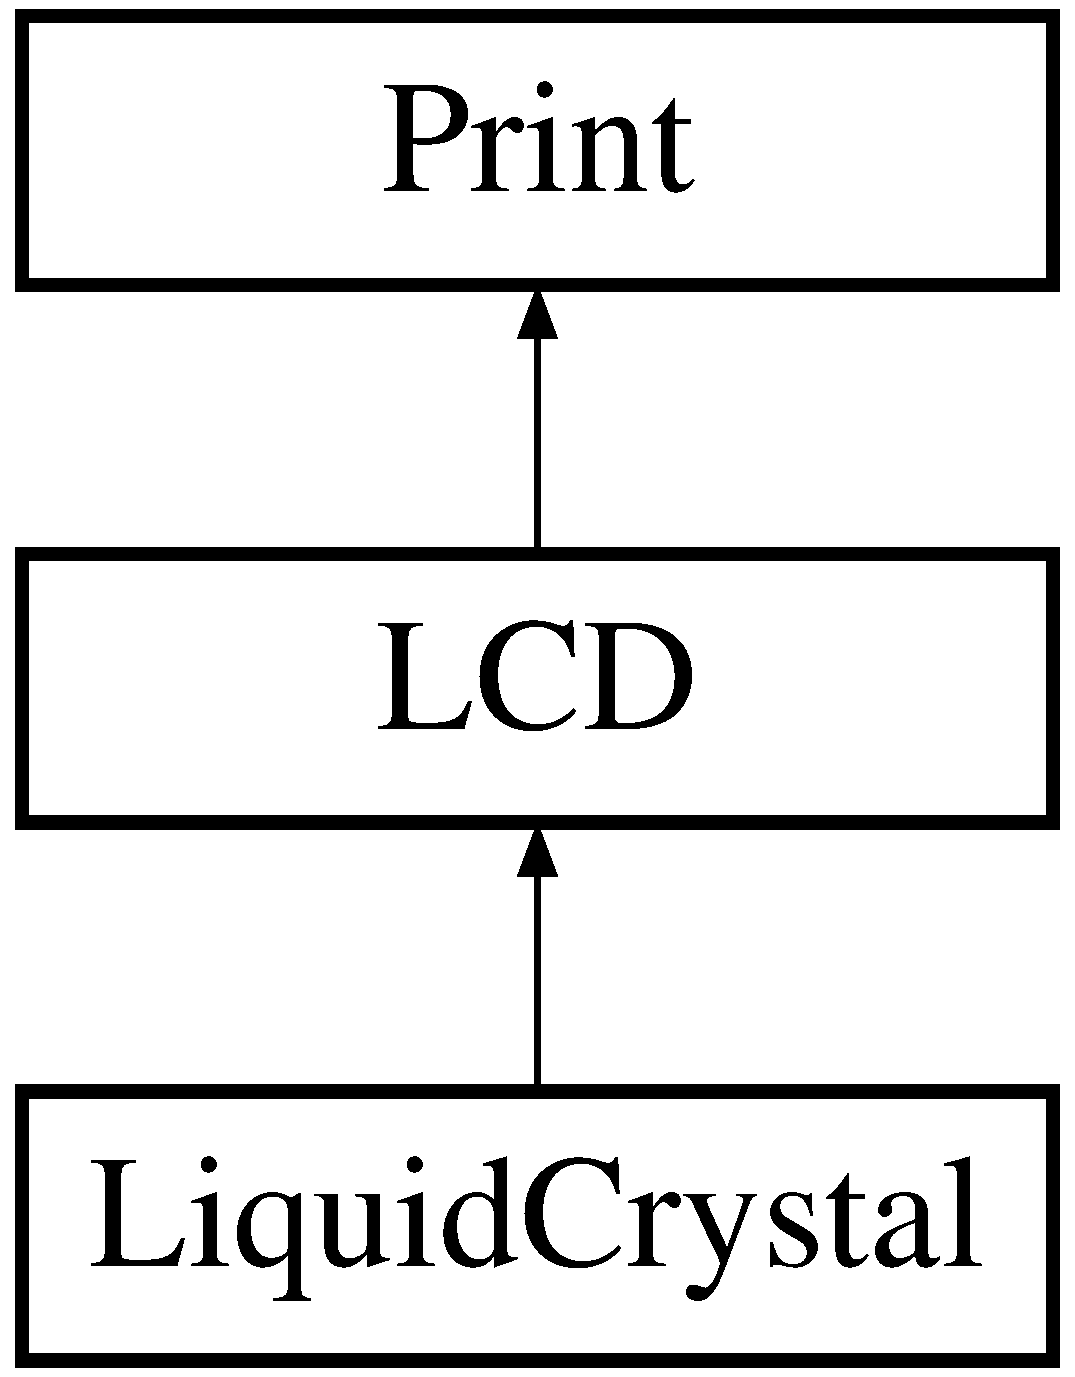
\includegraphics[height=3.000000cm]{class_liquid_crystal}
\end{center}
\end{figure}
\subsection*{Public Member Functions}
\begin{DoxyCompactItemize}
\item 
\hyperlink{class_liquid_crystal_a49d2bd8d26031a1c83bcbd73978a1686}{Liquid\+Crystal} (uint8\+\_\+t rs, uint8\+\_\+t enable, uint8\+\_\+t d0, uint8\+\_\+t d1, uint8\+\_\+t d2, uint8\+\_\+t d3, uint8\+\_\+t d4, uint8\+\_\+t d5, uint8\+\_\+t d6, uint8\+\_\+t d7)
\item 
\hypertarget{class_liquid_crystal_a30e3d865c4b4a003a36cb45903f93644}{}{\bfseries Liquid\+Crystal} (uint8\+\_\+t rs, uint8\+\_\+t rw, uint8\+\_\+t enable, uint8\+\_\+t d0, uint8\+\_\+t d1, uint8\+\_\+t d2, uint8\+\_\+t d3, uint8\+\_\+t d4, uint8\+\_\+t d5, uint8\+\_\+t d6, uint8\+\_\+t d7)\label{class_liquid_crystal_a30e3d865c4b4a003a36cb45903f93644}

\item 
\hypertarget{class_liquid_crystal_aff2330186495fde93370d46c0ca2cbf0}{}{\bfseries Liquid\+Crystal} (uint8\+\_\+t rs, uint8\+\_\+t enable, uint8\+\_\+t d0, uint8\+\_\+t d1, uint8\+\_\+t d2, uint8\+\_\+t d3, uint8\+\_\+t d4, uint8\+\_\+t d5, uint8\+\_\+t d6, uint8\+\_\+t d7, uint8\+\_\+t backlight\+Pin, t\+\_\+backligh\+Pol pol)\label{class_liquid_crystal_aff2330186495fde93370d46c0ca2cbf0}

\item 
\hypertarget{class_liquid_crystal_ae0c3c8f7661634b1400f00a1c9c02c26}{}{\bfseries Liquid\+Crystal} (uint8\+\_\+t rs, uint8\+\_\+t rw, uint8\+\_\+t enable, uint8\+\_\+t d0, uint8\+\_\+t d1, uint8\+\_\+t d2, uint8\+\_\+t d3, uint8\+\_\+t d4, uint8\+\_\+t d5, uint8\+\_\+t d6, uint8\+\_\+t d7, uint8\+\_\+t backlight\+Pin, t\+\_\+backligh\+Pol pol)\label{class_liquid_crystal_ae0c3c8f7661634b1400f00a1c9c02c26}

\item 
\hyperlink{class_liquid_crystal_a0a0a8dfa7a2e775a031fd65f5c6366ec}{Liquid\+Crystal} (uint8\+\_\+t rs, uint8\+\_\+t rw, uint8\+\_\+t enable, uint8\+\_\+t d0, uint8\+\_\+t d1, uint8\+\_\+t d2, uint8\+\_\+t d3)
\item 
\hypertarget{class_liquid_crystal_a23124e6dd5ac4a9b6147629b96e91953}{}{\bfseries Liquid\+Crystal} (uint8\+\_\+t rs, uint8\+\_\+t enable, uint8\+\_\+t d0, uint8\+\_\+t d1, uint8\+\_\+t d2, uint8\+\_\+t d3)\label{class_liquid_crystal_a23124e6dd5ac4a9b6147629b96e91953}

\item 
\hypertarget{class_liquid_crystal_a8b90122c67a6d14b967c8a11ba490670}{}{\bfseries Liquid\+Crystal} (uint8\+\_\+t rs, uint8\+\_\+t rw, uint8\+\_\+t enable, uint8\+\_\+t d0, uint8\+\_\+t d1, uint8\+\_\+t d2, uint8\+\_\+t d3, uint8\+\_\+t backlight\+Pin, t\+\_\+backligh\+Pol pol)\label{class_liquid_crystal_a8b90122c67a6d14b967c8a11ba490670}

\item 
\hypertarget{class_liquid_crystal_a52a4de3d866e347208a32dfc9d797729}{}{\bfseries Liquid\+Crystal} (uint8\+\_\+t rs, uint8\+\_\+t enable, uint8\+\_\+t d0, uint8\+\_\+t d1, uint8\+\_\+t d2, uint8\+\_\+t d3, uint8\+\_\+t backlight\+Pin, t\+\_\+backligh\+Pol pol)\label{class_liquid_crystal_a52a4de3d866e347208a32dfc9d797729}

\item 
virtual void \hyperlink{class_liquid_crystal_a56142f8b3753bedd133e4139e5eb5089}{send} (uint8\+\_\+t value, uint8\+\_\+t mode)
\item 
void \hyperlink{class_liquid_crystal_a63740dc1198d8169a39d9c6daff0efc9}{set\+Backlight\+Pin} (uint8\+\_\+t pin, t\+\_\+backligh\+Pol pol)
\item 
void \hyperlink{class_liquid_crystal_aa2b898366e1c656ac313b9007c98cebd}{set\+Backlight} (uint8\+\_\+t value)
\end{DoxyCompactItemize}
\subsection*{Additional Inherited Members}


\subsection{Constructor \& Destructor Documentation}
\hypertarget{class_liquid_crystal_a49d2bd8d26031a1c83bcbd73978a1686}{}\index{Liquid\+Crystal@{Liquid\+Crystal}!Liquid\+Crystal@{Liquid\+Crystal}}
\index{Liquid\+Crystal@{Liquid\+Crystal}!Liquid\+Crystal@{Liquid\+Crystal}}
\subsubsection[{Liquid\+Crystal}]{\setlength{\rightskip}{0pt plus 5cm}Liquid\+Crystal\+::\+Liquid\+Crystal (
\begin{DoxyParamCaption}
\item[{uint8\+\_\+t}]{rs, }
\item[{uint8\+\_\+t}]{enable, }
\item[{uint8\+\_\+t}]{d0, }
\item[{uint8\+\_\+t}]{d1, }
\item[{uint8\+\_\+t}]{d2, }
\item[{uint8\+\_\+t}]{d3, }
\item[{uint8\+\_\+t}]{d4, }
\item[{uint8\+\_\+t}]{d5, }
\item[{uint8\+\_\+t}]{d6, }
\item[{uint8\+\_\+t}]{d7}
\end{DoxyParamCaption}
)}\label{class_liquid_crystal_a49d2bd8d26031a1c83bcbd73978a1686}
8 bit \hyperlink{class_l_c_d}{L\+C\+D} constructors.  Defines the pin assignment that the \hyperlink{class_l_c_d}{L\+C\+D} will have. The constructor does not initialize the \hyperlink{class_l_c_d}{L\+C\+D}. \hypertarget{class_liquid_crystal_a0a0a8dfa7a2e775a031fd65f5c6366ec}{}\index{Liquid\+Crystal@{Liquid\+Crystal}!Liquid\+Crystal@{Liquid\+Crystal}}
\index{Liquid\+Crystal@{Liquid\+Crystal}!Liquid\+Crystal@{Liquid\+Crystal}}
\subsubsection[{Liquid\+Crystal}]{\setlength{\rightskip}{0pt plus 5cm}Liquid\+Crystal\+::\+Liquid\+Crystal (
\begin{DoxyParamCaption}
\item[{uint8\+\_\+t}]{rs, }
\item[{uint8\+\_\+t}]{rw, }
\item[{uint8\+\_\+t}]{enable, }
\item[{uint8\+\_\+t}]{d0, }
\item[{uint8\+\_\+t}]{d1, }
\item[{uint8\+\_\+t}]{d2, }
\item[{uint8\+\_\+t}]{d3}
\end{DoxyParamCaption}
)}\label{class_liquid_crystal_a0a0a8dfa7a2e775a031fd65f5c6366ec}
4 bit \hyperlink{class_l_c_d}{L\+C\+D} constructors.  Defines the pin assignment that the \hyperlink{class_l_c_d}{L\+C\+D} will have. The constructor does not initialize the \hyperlink{class_l_c_d}{L\+C\+D}. 

\subsection{Member Function Documentation}
\hypertarget{class_liquid_crystal_a56142f8b3753bedd133e4139e5eb5089}{}\index{Liquid\+Crystal@{Liquid\+Crystal}!send@{send}}
\index{send@{send}!Liquid\+Crystal@{Liquid\+Crystal}}
\subsubsection[{send}]{\setlength{\rightskip}{0pt plus 5cm}void Liquid\+Crystal\+::send (
\begin{DoxyParamCaption}
\item[{uint8\+\_\+t}]{value, }
\item[{uint8\+\_\+t}]{mode}
\end{DoxyParamCaption}
)\hspace{0.3cm}{\ttfamily [virtual]}}\label{class_liquid_crystal_a56142f8b3753bedd133e4139e5eb5089}
Send a particular value to the \hyperlink{class_l_c_d}{L\+C\+D}.  Sends a particular value to the \hyperlink{class_l_c_d}{L\+C\+D} for writing to the \hyperlink{class_l_c_d}{L\+C\+D} or as an \hyperlink{class_l_c_d}{L\+C\+D} command.

Users should never call this method.


\begin{DoxyParams}{Parameters}
{\em value} & Value to send to the \hyperlink{class_l_c_d}{L\+C\+D}. \\
\hline
\end{DoxyParams}
\begin{DoxyReturn}{Returns}
mode L\+O\+W -\/ write to the \hyperlink{class_l_c_d}{L\+C\+D} C\+G\+R\+A\+M, H\+I\+G\+H -\/ write a command to the \hyperlink{class_l_c_d}{L\+C\+D}. 
\end{DoxyReturn}


Reimplemented from \hyperlink{class_l_c_d}{L\+C\+D}.

\hypertarget{class_liquid_crystal_aa2b898366e1c656ac313b9007c98cebd}{}\index{Liquid\+Crystal@{Liquid\+Crystal}!set\+Backlight@{set\+Backlight}}
\index{set\+Backlight@{set\+Backlight}!Liquid\+Crystal@{Liquid\+Crystal}}
\subsubsection[{set\+Backlight}]{\setlength{\rightskip}{0pt plus 5cm}void Liquid\+Crystal\+::set\+Backlight (
\begin{DoxyParamCaption}
\item[{uint8\+\_\+t}]{value}
\end{DoxyParamCaption}
)\hspace{0.3cm}{\ttfamily [virtual]}}\label{class_liquid_crystal_aa2b898366e1c656ac313b9007c98cebd}
Switch-\/on/off the \hyperlink{class_l_c_d}{L\+C\+D} backlight.  Switch-\/on/off the \hyperlink{class_l_c_d}{L\+C\+D} backlight. The set\+Backlight\+Pin has to be called before setting the backlight for this method to work. \begin{DoxySeeAlso}{See also}
\hyperlink{class_liquid_crystal_a63740dc1198d8169a39d9c6daff0efc9}{set\+Backlight\+Pin}. For dimming control of the \hyperlink{class_l_c_d_aba8867fe2210cbfa8db869208709be10}{backlight}, the configuration pin must be a P\+W\+M output pin. Dim control is achieved by passing a value from 1 to 255 as a parameter. If the pin configured when calling the \hyperlink{class_liquid_crystal_a63740dc1198d8169a39d9c6daff0efc9}{set\+Backlight\+Pin} does not support P\+W\+M, then\+: (0) \hyperlink{class_l_c_d_aba8867fe2210cbfa8db869208709be10}{backlight} \hyperlink{class_l_c_d_a191639be183be1476c9bfe6d455d23b2}{off}, (1..255) \hyperlink{class_l_c_d_aba8867fe2210cbfa8db869208709be10}{backlight} \hyperlink{class_l_c_d_a718da3a638deb59bd1c7a5222a52d98a}{on}.
\end{DoxySeeAlso}

\begin{DoxyParams}{Parameters}
{\em value} & backlight value. 0\+: off, 1..255\+: dim control of the backlight. For negative logic 255\+: off, 254..0\+: dim control. \\
\hline
\end{DoxyParams}


Reimplemented from \hyperlink{class_l_c_d_a3305570d7b37eb93f2cf840263c15828}{L\+C\+D}.

\hypertarget{class_liquid_crystal_a63740dc1198d8169a39d9c6daff0efc9}{}\index{Liquid\+Crystal@{Liquid\+Crystal}!set\+Backlight\+Pin@{set\+Backlight\+Pin}}
\index{set\+Backlight\+Pin@{set\+Backlight\+Pin}!Liquid\+Crystal@{Liquid\+Crystal}}
\subsubsection[{set\+Backlight\+Pin}]{\setlength{\rightskip}{0pt plus 5cm}void Liquid\+Crystal\+::set\+Backlight\+Pin (
\begin{DoxyParamCaption}
\item[{uint8\+\_\+t}]{pin, }
\item[{t\+\_\+backligh\+Pol}]{pol}
\end{DoxyParamCaption}
)\hspace{0.3cm}{\ttfamily [virtual]}}\label{class_liquid_crystal_a63740dc1198d8169a39d9c6daff0efc9}
Sets the pin to control the backlight.  Sets the pin in the device to control the backlight.


\begin{DoxyParams}{Parameters}
{\em pin} & pin assigned to the backlight \\
\hline
{\em pol} & backlight pin control polarity (P\+O\+S\+I\+T\+I\+V\+E, N\+E\+G\+A\+T\+I\+V\+E). \\
\hline
\end{DoxyParams}


Reimplemented from \hyperlink{class_l_c_d_a53f4ee9b39d9ab3d7ae4d9f8dedca3bc}{L\+C\+D}.



The documentation for this class was generated from the following files\+:\begin{DoxyCompactItemize}
\item 
Libraries/\+Liquid\+Crystal/Liquid\+Crystal.\+h\item 
Libraries/\+Liquid\+Crystal/Liquid\+Crystal.\+cpp\end{DoxyCompactItemize}

\hypertarget{class_liquid_crystal___i2_c}{}\section{Liquid\+Crystal\+\_\+\+I2\+C Class Reference}
\label{class_liquid_crystal___i2_c}\index{Liquid\+Crystal\+\_\+\+I2\+C@{Liquid\+Crystal\+\_\+\+I2\+C}}
Inheritance diagram for Liquid\+Crystal\+\_\+\+I2\+C\+:\begin{figure}[H]
\begin{center}
\leavevmode
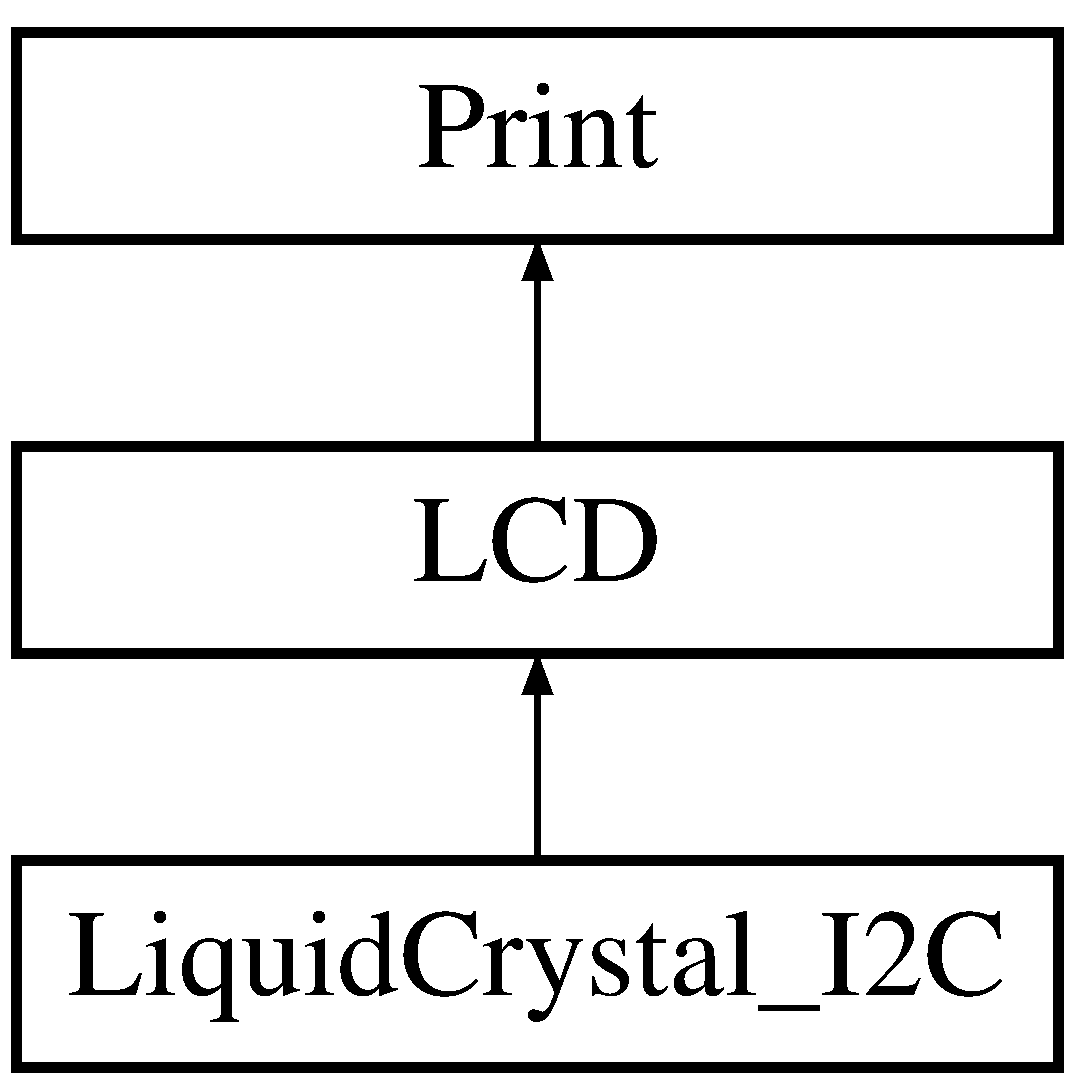
\includegraphics[height=3.000000cm]{class_liquid_crystal___i2_c}
\end{center}
\end{figure}
\subsection*{Public Member Functions}
\begin{DoxyCompactItemize}
\item 
\hyperlink{class_liquid_crystal___i2_c_aac537d195557e0b8afac1a71441a484c}{Liquid\+Crystal\+\_\+\+I2\+C} (uint8\+\_\+t lcd\+\_\+\+Addr)
\item 
\hypertarget{class_liquid_crystal___i2_c_a9fc9bc519ebbf7503dadc11622e02ed6}{}{\bfseries Liquid\+Crystal\+\_\+\+I2\+C} (uint8\+\_\+t lcd\+\_\+\+Addr, uint8\+\_\+t backligh\+Pin, t\+\_\+backligh\+Pol pol)\label{class_liquid_crystal___i2_c_a9fc9bc519ebbf7503dadc11622e02ed6}

\item 
\hyperlink{class_liquid_crystal___i2_c_a517f8847ebf09f0eacfb9c7232975fce}{Liquid\+Crystal\+\_\+\+I2\+C} (uint8\+\_\+t lcd\+\_\+\+Addr, uint8\+\_\+t En, uint8\+\_\+t Rw, uint8\+\_\+t Rs)
\item 
\hypertarget{class_liquid_crystal___i2_c_add1f2da7de4ec9b9cd5c9b5fab712464}{}{\bfseries Liquid\+Crystal\+\_\+\+I2\+C} (uint8\+\_\+t lcd\+\_\+\+Addr, uint8\+\_\+t En, uint8\+\_\+t Rw, uint8\+\_\+t Rs, uint8\+\_\+t backligh\+Pin, t\+\_\+backligh\+Pol pol)\label{class_liquid_crystal___i2_c_add1f2da7de4ec9b9cd5c9b5fab712464}

\item 
\hyperlink{class_liquid_crystal___i2_c_a7d9b54d3a91fa0e0e50db27cda6b4654}{Liquid\+Crystal\+\_\+\+I2\+C} (uint8\+\_\+t lcd\+\_\+\+Addr, uint8\+\_\+t En, uint8\+\_\+t Rw, uint8\+\_\+t Rs, uint8\+\_\+t d4, uint8\+\_\+t d5, uint8\+\_\+t d6, uint8\+\_\+t d7)
\item 
\hypertarget{class_liquid_crystal___i2_c_ab15622287533de7a47f3e2012ebf18be}{}{\bfseries Liquid\+Crystal\+\_\+\+I2\+C} (uint8\+\_\+t lcd\+\_\+\+Addr, uint8\+\_\+t En, uint8\+\_\+t Rw, uint8\+\_\+t Rs, uint8\+\_\+t d4, uint8\+\_\+t d5, uint8\+\_\+t d6, uint8\+\_\+t d7, uint8\+\_\+t backligh\+Pin, t\+\_\+backligh\+Pol pol)\label{class_liquid_crystal___i2_c_ab15622287533de7a47f3e2012ebf18be}

\item 
virtual void \hyperlink{class_liquid_crystal___i2_c_aeee2ada537f0cfbfda8613324b57c4a6}{begin} (uint8\+\_\+t cols, uint8\+\_\+t rows, uint8\+\_\+t charsize=L\+C\+D\+\_\+5x8\+D\+O\+T\+S)
\item 
virtual void \hyperlink{class_liquid_crystal___i2_c_a8bf1fab7efe13e8b17b96c42d1f810b4}{send} (uint8\+\_\+t value, uint8\+\_\+t mode)
\item 
void \hyperlink{class_liquid_crystal___i2_c_a2eaf86f62d1f169b3763b03fbf88f70b}{set\+Backlight\+Pin} (uint8\+\_\+t value, t\+\_\+backligh\+Pol pol)
\item 
void \hyperlink{class_liquid_crystal___i2_c_af11b8fa0082616e2b6e6e4238589d8a8}{set\+Backlight} (uint8\+\_\+t value)
\end{DoxyCompactItemize}
\subsection*{Additional Inherited Members}


\subsection{Constructor \& Destructor Documentation}
\hypertarget{class_liquid_crystal___i2_c_aac537d195557e0b8afac1a71441a484c}{}\index{Liquid\+Crystal\+\_\+\+I2\+C@{Liquid\+Crystal\+\_\+\+I2\+C}!Liquid\+Crystal\+\_\+\+I2\+C@{Liquid\+Crystal\+\_\+\+I2\+C}}
\index{Liquid\+Crystal\+\_\+\+I2\+C@{Liquid\+Crystal\+\_\+\+I2\+C}!Liquid\+Crystal\+\_\+\+I2\+C@{Liquid\+Crystal\+\_\+\+I2\+C}}
\subsubsection[{Liquid\+Crystal\+\_\+\+I2\+C}]{\setlength{\rightskip}{0pt plus 5cm}Liquid\+Crystal\+\_\+\+I2\+C\+::\+Liquid\+Crystal\+\_\+\+I2\+C (
\begin{DoxyParamCaption}
\item[{uint8\+\_\+t}]{lcd\+\_\+\+Addr}
\end{DoxyParamCaption}
)}\label{class_liquid_crystal___i2_c_aac537d195557e0b8afac1a71441a484c}
Class constructor.  Initializes class variables and defines the I2\+C address of the \hyperlink{class_l_c_d}{L\+C\+D}. The constructor does not initialize the \hyperlink{class_l_c_d}{L\+C\+D}.


\begin{DoxyParams}{Parameters}
{\em lcd\+\_\+\+Addr\mbox{[}in\mbox{]}} & I2\+C address of the I\+O expansion module. For I2\+C\+L\+C\+Dextra\+I\+O, the address can be configured using the on board jumpers. \\
\hline
\end{DoxyParams}
\hypertarget{class_liquid_crystal___i2_c_a517f8847ebf09f0eacfb9c7232975fce}{}\index{Liquid\+Crystal\+\_\+\+I2\+C@{Liquid\+Crystal\+\_\+\+I2\+C}!Liquid\+Crystal\+\_\+\+I2\+C@{Liquid\+Crystal\+\_\+\+I2\+C}}
\index{Liquid\+Crystal\+\_\+\+I2\+C@{Liquid\+Crystal\+\_\+\+I2\+C}!Liquid\+Crystal\+\_\+\+I2\+C@{Liquid\+Crystal\+\_\+\+I2\+C}}
\subsubsection[{Liquid\+Crystal\+\_\+\+I2\+C}]{\setlength{\rightskip}{0pt plus 5cm}Liquid\+Crystal\+\_\+\+I2\+C\+::\+Liquid\+Crystal\+\_\+\+I2\+C (
\begin{DoxyParamCaption}
\item[{uint8\+\_\+t}]{lcd\+\_\+\+Addr, }
\item[{uint8\+\_\+t}]{En, }
\item[{uint8\+\_\+t}]{Rw, }
\item[{uint8\+\_\+t}]{Rs}
\end{DoxyParamCaption}
)}\label{class_liquid_crystal___i2_c_a517f8847ebf09f0eacfb9c7232975fce}
Class constructor.  Initializes class variables and defines the I2\+C address of the \hyperlink{class_l_c_d}{L\+C\+D}. The constructor does not initialize the \hyperlink{class_l_c_d}{L\+C\+D}.


\begin{DoxyParams}{Parameters}
{\em lcd\+\_\+\+Addr\mbox{[}in\mbox{]}} & I2\+C address of the I\+O expansion module. For I2\+C\+L\+C\+Dextra\+I\+O, the address can be configured using the on board jumpers. \\
\hline
{\em En\mbox{[}in\mbox{]}} & \hyperlink{class_l_c_d}{L\+C\+D} En (Enable) pin connected to the I\+O extender module \\
\hline
{\em Rw\mbox{[}in\mbox{]}} & \hyperlink{class_l_c_d}{L\+C\+D} Rw (Read/write) pin connected to the I\+O extender module \\
\hline
{\em Rs\mbox{[}in\mbox{]}} & \hyperlink{class_l_c_d}{L\+C\+D} Rs (Reset) pin connected to the I\+O extender module \\
\hline
\end{DoxyParams}
\hypertarget{class_liquid_crystal___i2_c_a7d9b54d3a91fa0e0e50db27cda6b4654}{}\index{Liquid\+Crystal\+\_\+\+I2\+C@{Liquid\+Crystal\+\_\+\+I2\+C}!Liquid\+Crystal\+\_\+\+I2\+C@{Liquid\+Crystal\+\_\+\+I2\+C}}
\index{Liquid\+Crystal\+\_\+\+I2\+C@{Liquid\+Crystal\+\_\+\+I2\+C}!Liquid\+Crystal\+\_\+\+I2\+C@{Liquid\+Crystal\+\_\+\+I2\+C}}
\subsubsection[{Liquid\+Crystal\+\_\+\+I2\+C}]{\setlength{\rightskip}{0pt plus 5cm}Liquid\+Crystal\+\_\+\+I2\+C\+::\+Liquid\+Crystal\+\_\+\+I2\+C (
\begin{DoxyParamCaption}
\item[{uint8\+\_\+t}]{lcd\+\_\+\+Addr, }
\item[{uint8\+\_\+t}]{En, }
\item[{uint8\+\_\+t}]{Rw, }
\item[{uint8\+\_\+t}]{Rs, }
\item[{uint8\+\_\+t}]{d4, }
\item[{uint8\+\_\+t}]{d5, }
\item[{uint8\+\_\+t}]{d6, }
\item[{uint8\+\_\+t}]{d7}
\end{DoxyParamCaption}
)}\label{class_liquid_crystal___i2_c_a7d9b54d3a91fa0e0e50db27cda6b4654}
Class constructor.  Initializes class variables and defines the I2\+C address of the \hyperlink{class_l_c_d}{L\+C\+D}. The constructor does not initialize the \hyperlink{class_l_c_d}{L\+C\+D}.


\begin{DoxyParams}{Parameters}
{\em lcd\+\_\+\+Addr\mbox{[}in\mbox{]}} & I2\+C address of the I\+O expansion module. For I2\+C\+L\+C\+Dextra\+I\+O, the address can be configured using the on board jumpers. \\
\hline
{\em En\mbox{[}in\mbox{]}} & \hyperlink{class_l_c_d}{L\+C\+D} En (Enable) pin connected to the I\+O extender module \\
\hline
{\em Rw\mbox{[}in\mbox{]}} & \hyperlink{class_l_c_d}{L\+C\+D} Rw (Read/write) pin connected to the I\+O extender module \\
\hline
{\em Rs\mbox{[}in\mbox{]}} & \hyperlink{class_l_c_d}{L\+C\+D} Rs (Reset) pin connected to the I\+O extender module \\
\hline
{\em d4\mbox{[}in\mbox{]}} & \hyperlink{class_l_c_d}{L\+C\+D} data 0 pin map on I\+O extender module \\
\hline
{\em d5\mbox{[}in\mbox{]}} & \hyperlink{class_l_c_d}{L\+C\+D} data 1 pin map on I\+O extender module \\
\hline
{\em d6\mbox{[}in\mbox{]}} & \hyperlink{class_l_c_d}{L\+C\+D} data 2 pin map on I\+O extender module \\
\hline
{\em d7\mbox{[}in\mbox{]}} & \hyperlink{class_l_c_d}{L\+C\+D} data 3 pin map on I\+O extender module \\
\hline
\end{DoxyParams}


\subsection{Member Function Documentation}
\hypertarget{class_liquid_crystal___i2_c_aeee2ada537f0cfbfda8613324b57c4a6}{}\index{Liquid\+Crystal\+\_\+\+I2\+C@{Liquid\+Crystal\+\_\+\+I2\+C}!begin@{begin}}
\index{begin@{begin}!Liquid\+Crystal\+\_\+\+I2\+C@{Liquid\+Crystal\+\_\+\+I2\+C}}
\subsubsection[{begin}]{\setlength{\rightskip}{0pt plus 5cm}void Liquid\+Crystal\+\_\+\+I2\+C\+::begin (
\begin{DoxyParamCaption}
\item[{uint8\+\_\+t}]{cols, }
\item[{uint8\+\_\+t}]{rows, }
\item[{uint8\+\_\+t}]{charsize = {\ttfamily LCD\+\_\+5x8DOTS}}
\end{DoxyParamCaption}
)\hspace{0.3cm}{\ttfamily [virtual]}}\label{class_liquid_crystal___i2_c_aeee2ada537f0cfbfda8613324b57c4a6}
\hyperlink{class_l_c_d}{L\+C\+D} initialization and associated H\+W.  Initializes the \hyperlink{class_l_c_d}{L\+C\+D} to a given size (col, row). This methods initializes the \hyperlink{class_l_c_d}{L\+C\+D}, therefore, it M\+U\+S\+T be called prior to using any other method from this class or parent class.

The begin method can be overloaded if necessary to initialize any H\+W that is implemented by a library and can\textquotesingle{}t be done during construction, here we use the Wire class.


\begin{DoxyParams}{Parameters}
{\em cols\mbox{[}in\mbox{]}} & the number of columns that the display has \\
\hline
{\em rows\mbox{[}in\mbox{]}} & the number of rows that the display has \\
\hline
{\em charsize\mbox{[}in\mbox{]}} & size of the characters of the \hyperlink{class_l_c_d}{L\+C\+D}\+: L\+C\+D\+\_\+5x8\+D\+O\+T\+S or L\+C\+D\+\_\+5x10\+D\+O\+T\+S. \\
\hline
\end{DoxyParams}


Reimplemented from \hyperlink{class_l_c_d_a3f587d1cbb2d59765ef60a5216b56fea}{L\+C\+D}.

\hypertarget{class_liquid_crystal___i2_c_a8bf1fab7efe13e8b17b96c42d1f810b4}{}\index{Liquid\+Crystal\+\_\+\+I2\+C@{Liquid\+Crystal\+\_\+\+I2\+C}!send@{send}}
\index{send@{send}!Liquid\+Crystal\+\_\+\+I2\+C@{Liquid\+Crystal\+\_\+\+I2\+C}}
\subsubsection[{send}]{\setlength{\rightskip}{0pt plus 5cm}void Liquid\+Crystal\+\_\+\+I2\+C\+::send (
\begin{DoxyParamCaption}
\item[{uint8\+\_\+t}]{value, }
\item[{uint8\+\_\+t}]{mode}
\end{DoxyParamCaption}
)\hspace{0.3cm}{\ttfamily [virtual]}}\label{class_liquid_crystal___i2_c_a8bf1fab7efe13e8b17b96c42d1f810b4}
Send a particular value to the \hyperlink{class_l_c_d}{L\+C\+D}.  Sends a particular value to the \hyperlink{class_l_c_d}{L\+C\+D} for writing to the \hyperlink{class_l_c_d}{L\+C\+D} or as an \hyperlink{class_l_c_d}{L\+C\+D} command.

Users should never call this method.


\begin{DoxyParams}{Parameters}
{\em value\mbox{[}in\mbox{]}} & Value to send to the \hyperlink{class_l_c_d}{L\+C\+D}. \\
\hline
{\em mode\mbox{[}in\mbox{]}} & D\+A\+T\+A -\/ write to the \hyperlink{class_l_c_d}{L\+C\+D} C\+G\+R\+A\+M, C\+O\+M\+M\+A\+N\+D -\/ write a command to the \hyperlink{class_l_c_d}{L\+C\+D}. \\
\hline
\end{DoxyParams}


Reimplemented from \hyperlink{class_l_c_d}{L\+C\+D}.

\hypertarget{class_liquid_crystal___i2_c_af11b8fa0082616e2b6e6e4238589d8a8}{}\index{Liquid\+Crystal\+\_\+\+I2\+C@{Liquid\+Crystal\+\_\+\+I2\+C}!set\+Backlight@{set\+Backlight}}
\index{set\+Backlight@{set\+Backlight}!Liquid\+Crystal\+\_\+\+I2\+C@{Liquid\+Crystal\+\_\+\+I2\+C}}
\subsubsection[{set\+Backlight}]{\setlength{\rightskip}{0pt plus 5cm}void Liquid\+Crystal\+\_\+\+I2\+C\+::set\+Backlight (
\begin{DoxyParamCaption}
\item[{uint8\+\_\+t}]{value}
\end{DoxyParamCaption}
)\hspace{0.3cm}{\ttfamily [virtual]}}\label{class_liquid_crystal___i2_c_af11b8fa0082616e2b6e6e4238589d8a8}
Switch-\/on/off the \hyperlink{class_l_c_d}{L\+C\+D} backlight.  Switch-\/on/off the \hyperlink{class_l_c_d}{L\+C\+D} backlight. The set\+Backlight\+Pin has to be called before setting the backlight for this method to work. \begin{DoxySeeAlso}{See also}
\hyperlink{class_liquid_crystal___i2_c_a2eaf86f62d1f169b3763b03fbf88f70b}{set\+Backlight\+Pin}.
\end{DoxySeeAlso}

\begin{DoxyParams}{Parameters}
{\em value} & backlight mode (H\+I\+G\+H$\vert$\+L\+O\+W) \\
\hline
\end{DoxyParams}


Reimplemented from \hyperlink{class_l_c_d_a3305570d7b37eb93f2cf840263c15828}{L\+C\+D}.

\hypertarget{class_liquid_crystal___i2_c_a2eaf86f62d1f169b3763b03fbf88f70b}{}\index{Liquid\+Crystal\+\_\+\+I2\+C@{Liquid\+Crystal\+\_\+\+I2\+C}!set\+Backlight\+Pin@{set\+Backlight\+Pin}}
\index{set\+Backlight\+Pin@{set\+Backlight\+Pin}!Liquid\+Crystal\+\_\+\+I2\+C@{Liquid\+Crystal\+\_\+\+I2\+C}}
\subsubsection[{set\+Backlight\+Pin}]{\setlength{\rightskip}{0pt plus 5cm}void Liquid\+Crystal\+\_\+\+I2\+C\+::set\+Backlight\+Pin (
\begin{DoxyParamCaption}
\item[{uint8\+\_\+t}]{value, }
\item[{t\+\_\+backligh\+Pol}]{pol = {\ttfamily POSITIVE}}
\end{DoxyParamCaption}
)\hspace{0.3cm}{\ttfamily [virtual]}}\label{class_liquid_crystal___i2_c_a2eaf86f62d1f169b3763b03fbf88f70b}
Sets the pin to control the backlight.  Sets the pin in the device to control the backlight. This device doesn\textquotesingle{}t support dimming backlight capability.


\begin{DoxyParams}{Parameters}
{\em 0} & backlight off, 1..255\+: backlight on. \\
\hline
\end{DoxyParams}


Reimplemented from \hyperlink{class_l_c_d_a53f4ee9b39d9ab3d7ae4d9f8dedca3bc}{L\+C\+D}.



The documentation for this class was generated from the following files\+:\begin{DoxyCompactItemize}
\item 
Libraries/\+Liquid\+Crystal/Liquid\+Crystal\+\_\+\+I2\+C.\+h\item 
Libraries/\+Liquid\+Crystal/Liquid\+Crystal\+\_\+\+I2\+C.\+cpp\end{DoxyCompactItemize}

\hypertarget{class_liquid_crystal___s_r}{}\section{Liquid\+Crystal\+\_\+\+S\+R Class Reference}
\label{class_liquid_crystal___s_r}\index{Liquid\+Crystal\+\_\+\+S\+R@{Liquid\+Crystal\+\_\+\+S\+R}}
Inheritance diagram for Liquid\+Crystal\+\_\+\+S\+R\+:\begin{figure}[H]
\begin{center}
\leavevmode
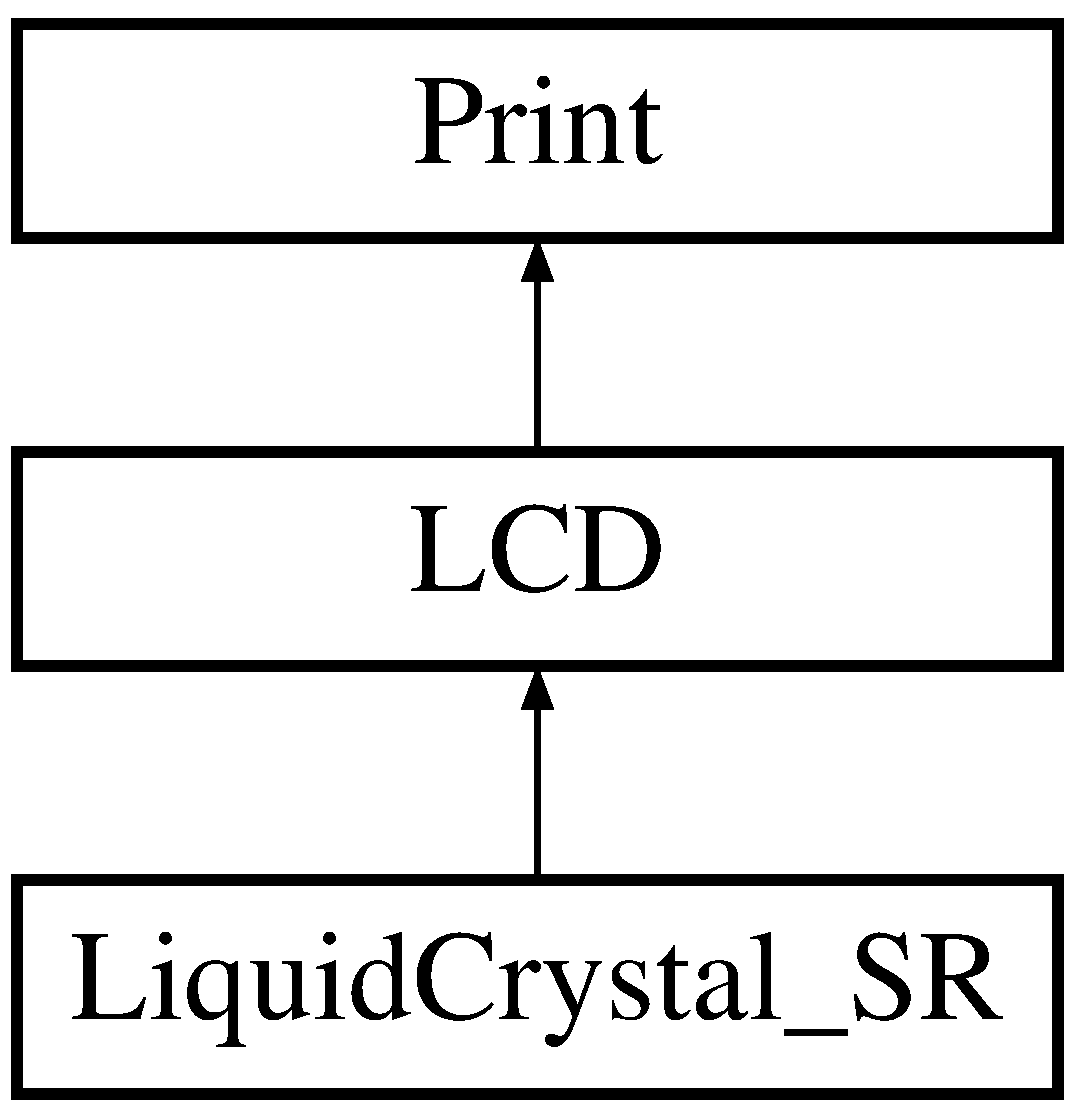
\includegraphics[height=3.000000cm]{class_liquid_crystal___s_r}
\end{center}
\end{figure}
\subsection*{Public Member Functions}
\begin{DoxyCompactItemize}
\item 
\hyperlink{class_liquid_crystal___s_r_ac3fe0b48f8d4c1c941d82d1333495cfc}{Liquid\+Crystal\+\_\+\+S\+R} (uint8\+\_\+t srdata, uint8\+\_\+t srclock, uint8\+\_\+t enable=T\+W\+O\+\_\+\+W\+I\+R\+E)
\item 
virtual void \hyperlink{class_liquid_crystal___s_r_a03821351a32db07cb7e42c8c11ce8d47}{send} (uint8\+\_\+t value, uint8\+\_\+t mode)
\item 
void \hyperlink{class_liquid_crystal___s_r_a5bfc0dcc1f042bcb59992493a3a7231d}{set\+Backlight\+Pin} (uint8\+\_\+t pin, t\+\_\+backligh\+Pol pol)
\item 
void \hyperlink{class_liquid_crystal___s_r_ad9f3e3f36257984c23fb508973e14535}{set\+Backlight} (uint8\+\_\+t mode)
\end{DoxyCompactItemize}
\subsection*{Additional Inherited Members}


\subsection{Constructor \& Destructor Documentation}
\hypertarget{class_liquid_crystal___s_r_ac3fe0b48f8d4c1c941d82d1333495cfc}{}\index{Liquid\+Crystal\+\_\+\+S\+R@{Liquid\+Crystal\+\_\+\+S\+R}!Liquid\+Crystal\+\_\+\+S\+R@{Liquid\+Crystal\+\_\+\+S\+R}}
\index{Liquid\+Crystal\+\_\+\+S\+R@{Liquid\+Crystal\+\_\+\+S\+R}!Liquid\+Crystal\+\_\+\+S\+R@{Liquid\+Crystal\+\_\+\+S\+R}}
\subsubsection[{Liquid\+Crystal\+\_\+\+S\+R}]{\setlength{\rightskip}{0pt plus 5cm}Liquid\+Crystal\+\_\+\+S\+R\+::\+Liquid\+Crystal\+\_\+\+S\+R (
\begin{DoxyParamCaption}
\item[{uint8\+\_\+t}]{srdata, }
\item[{uint8\+\_\+t}]{srclock, }
\item[{uint8\+\_\+t}]{enable = {\ttfamily TWO\+\_\+WIRE}}
\end{DoxyParamCaption}
)}\label{class_liquid_crystal___s_r_ac3fe0b48f8d4c1c941d82d1333495cfc}
\hyperlink{class_l_c_d}{L\+C\+D} S\+H\+I\+F\+T R\+E\+G\+I\+S\+T\+E\+R constructors.  Defines the pin assignment that the \hyperlink{class_l_c_d}{L\+C\+D} will have. The constructor does not initialize the \hyperlink{class_l_c_d}{L\+C\+D}. Assuming 1 line 8 pixel high font.


\begin{DoxyParams}{Parameters}
{\em srdata\mbox{[}in\mbox{]}} & pin for shiftregister data line. \\
\hline
{\em srclock\mbox{[}in\mbox{]}} & pin for shiftregister clock line. \\
\hline
{\em enable\mbox{[}in\mbox{]}} & optional direct enable pin for the \hyperlink{class_l_c_d}{L\+C\+D} \\
\hline
\end{DoxyParams}


\subsection{Member Function Documentation}
\hypertarget{class_liquid_crystal___s_r_a03821351a32db07cb7e42c8c11ce8d47}{}\index{Liquid\+Crystal\+\_\+\+S\+R@{Liquid\+Crystal\+\_\+\+S\+R}!send@{send}}
\index{send@{send}!Liquid\+Crystal\+\_\+\+S\+R@{Liquid\+Crystal\+\_\+\+S\+R}}
\subsubsection[{send}]{\setlength{\rightskip}{0pt plus 5cm}void Liquid\+Crystal\+\_\+\+S\+R\+::send (
\begin{DoxyParamCaption}
\item[{uint8\+\_\+t}]{value, }
\item[{uint8\+\_\+t}]{mode}
\end{DoxyParamCaption}
)\hspace{0.3cm}{\ttfamily [virtual]}}\label{class_liquid_crystal___s_r_a03821351a32db07cb7e42c8c11ce8d47}
Send a particular value to the \hyperlink{class_l_c_d}{L\+C\+D}.  Sends a particular value to the \hyperlink{class_l_c_d}{L\+C\+D} for writing to the \hyperlink{class_l_c_d}{L\+C\+D} or as an \hyperlink{class_l_c_d}{L\+C\+D} command using the shift register.

Users should never call this method.


\begin{DoxyParams}{Parameters}
{\em value\mbox{[}in\mbox{]}} & Value to send to the \hyperlink{class_l_c_d}{L\+C\+D}. \\
\hline
\end{DoxyParams}
\begin{DoxyReturn}{Returns}
mode L\+O\+W -\/ write to the \hyperlink{class_l_c_d}{L\+C\+D} C\+G\+R\+A\+M, H\+I\+G\+H -\/ write a command to the \hyperlink{class_l_c_d}{L\+C\+D}. 
\end{DoxyReturn}


Reimplemented from \hyperlink{class_l_c_d}{L\+C\+D}.

\hypertarget{class_liquid_crystal___s_r_ad9f3e3f36257984c23fb508973e14535}{}\index{Liquid\+Crystal\+\_\+\+S\+R@{Liquid\+Crystal\+\_\+\+S\+R}!set\+Backlight@{set\+Backlight}}
\index{set\+Backlight@{set\+Backlight}!Liquid\+Crystal\+\_\+\+S\+R@{Liquid\+Crystal\+\_\+\+S\+R}}
\subsubsection[{set\+Backlight}]{\setlength{\rightskip}{0pt plus 5cm}void Liquid\+Crystal\+\_\+\+S\+R\+::set\+Backlight (
\begin{DoxyParamCaption}
\item[{uint8\+\_\+t}]{mode}
\end{DoxyParamCaption}
)\hspace{0.3cm}{\ttfamily [virtual]}}\label{class_liquid_crystal___s_r_ad9f3e3f36257984c23fb508973e14535}
Switch-\/on/off the \hyperlink{class_l_c_d}{L\+C\+D} backlight.  Switch-\/on/off the \hyperlink{class_l_c_d}{L\+C\+D} backlight. The set\+Backlight\+Pin has to be called before setting the backlight for this method to work. \begin{DoxySeeAlso}{See also}
\hyperlink{class_liquid_crystal___s_r_a5bfc0dcc1f042bcb59992493a3a7231d}{set\+Backlight\+Pin}.
\end{DoxySeeAlso}

\begin{DoxyParams}{Parameters}
{\em mode} & backlight mode (H\+I\+G\+H$\vert$\+L\+O\+W) \\
\hline
\end{DoxyParams}


Reimplemented from \hyperlink{class_l_c_d_a3305570d7b37eb93f2cf840263c15828}{L\+C\+D}.

\hypertarget{class_liquid_crystal___s_r_a5bfc0dcc1f042bcb59992493a3a7231d}{}\index{Liquid\+Crystal\+\_\+\+S\+R@{Liquid\+Crystal\+\_\+\+S\+R}!set\+Backlight\+Pin@{set\+Backlight\+Pin}}
\index{set\+Backlight\+Pin@{set\+Backlight\+Pin}!Liquid\+Crystal\+\_\+\+S\+R@{Liquid\+Crystal\+\_\+\+S\+R}}
\subsubsection[{set\+Backlight\+Pin}]{\setlength{\rightskip}{0pt plus 5cm}void Liquid\+Crystal\+\_\+\+S\+R\+::set\+Backlight\+Pin (
\begin{DoxyParamCaption}
\item[{uint8\+\_\+t}]{pin, }
\item[{t\+\_\+backligh\+Pol}]{pol}
\end{DoxyParamCaption}
)\hspace{0.3cm}{\ttfamily [virtual]}}\label{class_liquid_crystal___s_r_a5bfc0dcc1f042bcb59992493a3a7231d}
Sets the pin to control the backlight.  Sets the pin in the device to control the backlight. \begin{DoxyWarning}{Warning}
Currently not supported
\end{DoxyWarning}

\begin{DoxyParams}{Parameters}
{\em mode} & backlight mode (H\+I\+G\+H$\vert$\+L\+O\+W) \\
\hline
{\em pol} & backlight polarity \\
\hline
\end{DoxyParams}


Reimplemented from \hyperlink{class_l_c_d_a53f4ee9b39d9ab3d7ae4d9f8dedca3bc}{L\+C\+D}.



The documentation for this class was generated from the following files\+:\begin{DoxyCompactItemize}
\item 
Libraries/\+Liquid\+Crystal/Liquid\+Crystal\+\_\+\+S\+R.\+h\item 
Libraries/\+Liquid\+Crystal/Liquid\+Crystal\+\_\+\+S\+R.\+cpp\end{DoxyCompactItemize}

\hypertarget{class_liquid_crystal___s_r2_w}{}\section{Liquid\+Crystal\+\_\+\+S\+R2\+W Class Reference}
\label{class_liquid_crystal___s_r2_w}\index{Liquid\+Crystal\+\_\+\+S\+R2\+W@{Liquid\+Crystal\+\_\+\+S\+R2\+W}}
Inheritance diagram for Liquid\+Crystal\+\_\+\+S\+R2\+W\+:\begin{figure}[H]
\begin{center}
\leavevmode
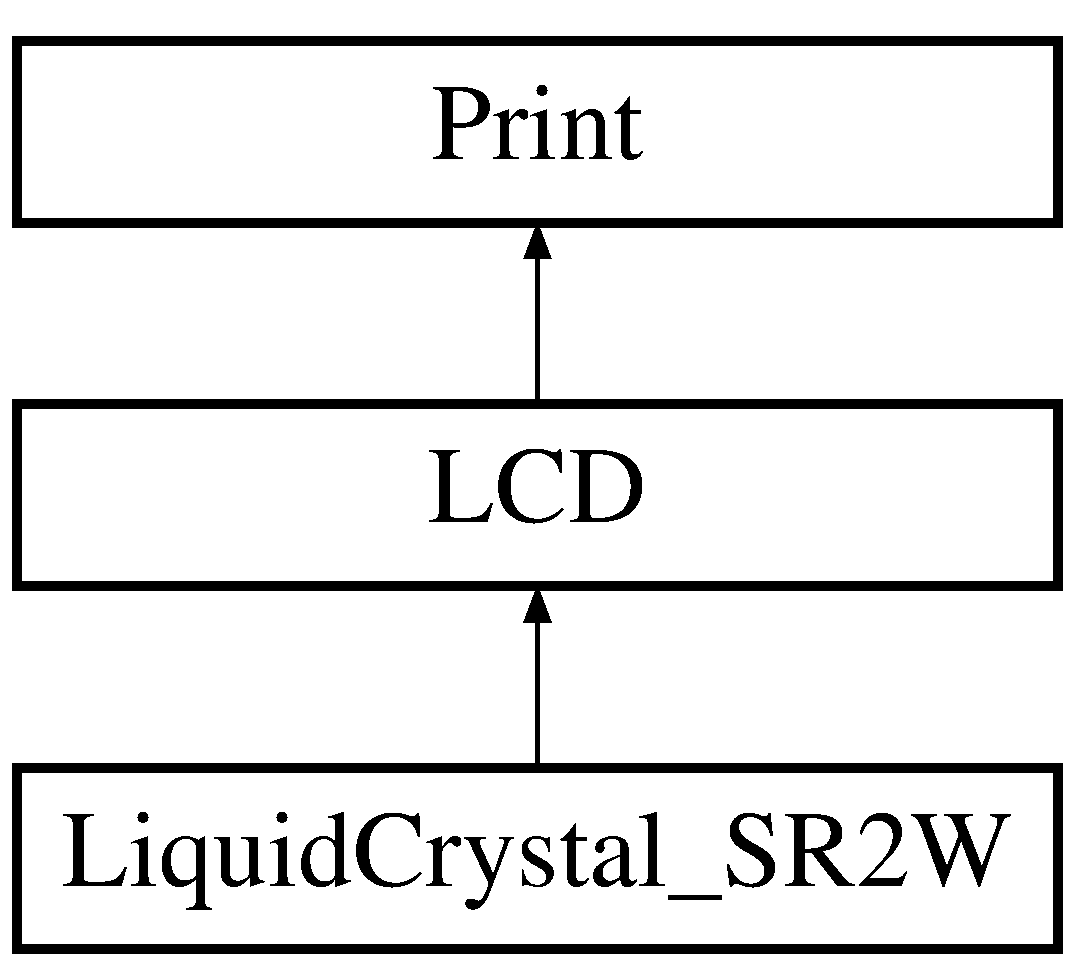
\includegraphics[height=3.000000cm]{class_liquid_crystal___s_r2_w}
\end{center}
\end{figure}
\subsection*{Public Member Functions}
\begin{DoxyCompactItemize}
\item 
\hyperlink{class_liquid_crystal___s_r2_w_af307fdf5c8feb757e965074dcdeb1dd3}{Liquid\+Crystal\+\_\+\+S\+R2\+W} (uint8\+\_\+t srdata, uint8\+\_\+t srclock, t\+\_\+backligh\+Pol blpol=P\+O\+S\+I\+T\+I\+V\+E)
\item 
virtual void \hyperlink{class_liquid_crystal___s_r2_w_a65dc6f261c319be8e56f3c1f6a5c877d}{send} (uint8\+\_\+t value, uint8\+\_\+t mode)
\item 
void \hyperlink{class_liquid_crystal___s_r2_w_a2158db27287c1564a03e7a1472beb3b6}{set\+Backlight} (uint8\+\_\+t mode)
\end{DoxyCompactItemize}
\subsection*{Additional Inherited Members}


\subsection{Constructor \& Destructor Documentation}
\hypertarget{class_liquid_crystal___s_r2_w_af307fdf5c8feb757e965074dcdeb1dd3}{}\index{Liquid\+Crystal\+\_\+\+S\+R2\+W@{Liquid\+Crystal\+\_\+\+S\+R2\+W}!Liquid\+Crystal\+\_\+\+S\+R2\+W@{Liquid\+Crystal\+\_\+\+S\+R2\+W}}
\index{Liquid\+Crystal\+\_\+\+S\+R2\+W@{Liquid\+Crystal\+\_\+\+S\+R2\+W}!Liquid\+Crystal\+\_\+\+S\+R2\+W@{Liquid\+Crystal\+\_\+\+S\+R2\+W}}
\subsubsection[{Liquid\+Crystal\+\_\+\+S\+R2\+W}]{\setlength{\rightskip}{0pt plus 5cm}Liquid\+Crystal\+\_\+\+S\+R2\+W\+::\+Liquid\+Crystal\+\_\+\+S\+R2\+W (
\begin{DoxyParamCaption}
\item[{uint8\+\_\+t}]{srdata, }
\item[{uint8\+\_\+t}]{srclock, }
\item[{t\+\_\+backligh\+Pol}]{blpol = {\ttfamily POSITIVE}}
\end{DoxyParamCaption}
)}\label{class_liquid_crystal___s_r2_w_af307fdf5c8feb757e965074dcdeb1dd3}
\hyperlink{class_l_c_d}{L\+C\+D} 2 wire S\+H\+I\+F\+T R\+E\+G\+I\+S\+T\+E\+R constructor.  Defines the pin assignments that connect to the shift register. The constructor does not initialize the \hyperlink{class_l_c_d}{L\+C\+D}. Assuming 1 line 8 pixel high font.


\begin{DoxyParams}{Parameters}
{\em srdata\mbox{[}in\mbox{]}} & Arduino pin for shift register data line. \\
\hline
{\em srclock\mbox{[}in\mbox{]}} & Arduino pin for shift register clock line. \\
\hline
{\em blpol\mbox{[}in\mbox{]}} & optional backlight polarity (default = P\+O\+S\+I\+T\+I\+V\+E) \\
\hline
\end{DoxyParams}


\subsection{Member Function Documentation}
\hypertarget{class_liquid_crystal___s_r2_w_a65dc6f261c319be8e56f3c1f6a5c877d}{}\index{Liquid\+Crystal\+\_\+\+S\+R2\+W@{Liquid\+Crystal\+\_\+\+S\+R2\+W}!send@{send}}
\index{send@{send}!Liquid\+Crystal\+\_\+\+S\+R2\+W@{Liquid\+Crystal\+\_\+\+S\+R2\+W}}
\subsubsection[{send}]{\setlength{\rightskip}{0pt plus 5cm}void Liquid\+Crystal\+\_\+\+S\+R2\+W\+::send (
\begin{DoxyParamCaption}
\item[{uint8\+\_\+t}]{value, }
\item[{uint8\+\_\+t}]{mode}
\end{DoxyParamCaption}
)\hspace{0.3cm}{\ttfamily [virtual]}}\label{class_liquid_crystal___s_r2_w_a65dc6f261c319be8e56f3c1f6a5c877d}
Send a particular value to the \hyperlink{class_l_c_d}{L\+C\+D}.  Sends a particular value to the \hyperlink{class_l_c_d}{L\+C\+D} for writing to the \hyperlink{class_l_c_d}{L\+C\+D} or as an \hyperlink{class_l_c_d}{L\+C\+D} command using the shift register.

Users should never call this method.


\begin{DoxyParams}{Parameters}
{\em value\mbox{[}in\mbox{]}} & Value to send to the \hyperlink{class_l_c_d}{L\+C\+D}. \\
\hline
{\em mode\mbox{[}in\mbox{]}} & D\+A\+T\+A=8bit data, C\+O\+M\+M\+A\+N\+D=8bit cmd, F\+O\+U\+R\+\_\+\+B\+I\+T\+S=4bit cmd the \hyperlink{class_l_c_d}{L\+C\+D}. \\
\hline
\end{DoxyParams}


Reimplemented from \hyperlink{class_l_c_d}{L\+C\+D}.

\hypertarget{class_liquid_crystal___s_r2_w_a2158db27287c1564a03e7a1472beb3b6}{}\index{Liquid\+Crystal\+\_\+\+S\+R2\+W@{Liquid\+Crystal\+\_\+\+S\+R2\+W}!set\+Backlight@{set\+Backlight}}
\index{set\+Backlight@{set\+Backlight}!Liquid\+Crystal\+\_\+\+S\+R2\+W@{Liquid\+Crystal\+\_\+\+S\+R2\+W}}
\subsubsection[{set\+Backlight}]{\setlength{\rightskip}{0pt plus 5cm}void Liquid\+Crystal\+\_\+\+S\+R2\+W\+::set\+Backlight (
\begin{DoxyParamCaption}
\item[{uint8\+\_\+t}]{mode}
\end{DoxyParamCaption}
)\hspace{0.3cm}{\ttfamily [virtual]}}\label{class_liquid_crystal___s_r2_w_a2158db27287c1564a03e7a1472beb3b6}
Switch-\/on/off the \hyperlink{class_l_c_d}{L\+C\+D} backlight.  Switch-\/on/off the \hyperlink{class_l_c_d}{L\+C\+D} backlight. The set\+Backlight\+Pin has to be called before setting the backlight for this method to work. \begin{DoxySeeAlso}{See also}
\hyperlink{class_l_c_d_a53f4ee9b39d9ab3d7ae4d9f8dedca3bc}{set\+Backlight\+Pin}.
\end{DoxySeeAlso}

\begin{DoxyParams}{Parameters}
{\em mode\mbox{[}in\mbox{]}} & backlight mode (0 off, non-\/zero on) \\
\hline
\end{DoxyParams}


Reimplemented from \hyperlink{class_l_c_d_a3305570d7b37eb93f2cf840263c15828}{L\+C\+D}.



The documentation for this class was generated from the following files\+:\begin{DoxyCompactItemize}
\item 
Libraries/\+Liquid\+Crystal/Liquid\+Crystal\+\_\+\+S\+R2\+W.\+h\item 
Libraries/\+Liquid\+Crystal/Liquid\+Crystal\+\_\+\+S\+R2\+W.\+cpp\end{DoxyCompactItemize}

\hypertarget{class_liquid_crystal___s_r3_w}{}\section{Liquid\+Crystal\+\_\+\+S\+R3\+W Class Reference}
\label{class_liquid_crystal___s_r3_w}\index{Liquid\+Crystal\+\_\+\+S\+R3\+W@{Liquid\+Crystal\+\_\+\+S\+R3\+W}}
Inheritance diagram for Liquid\+Crystal\+\_\+\+S\+R3\+W\+:\begin{figure}[H]
\begin{center}
\leavevmode
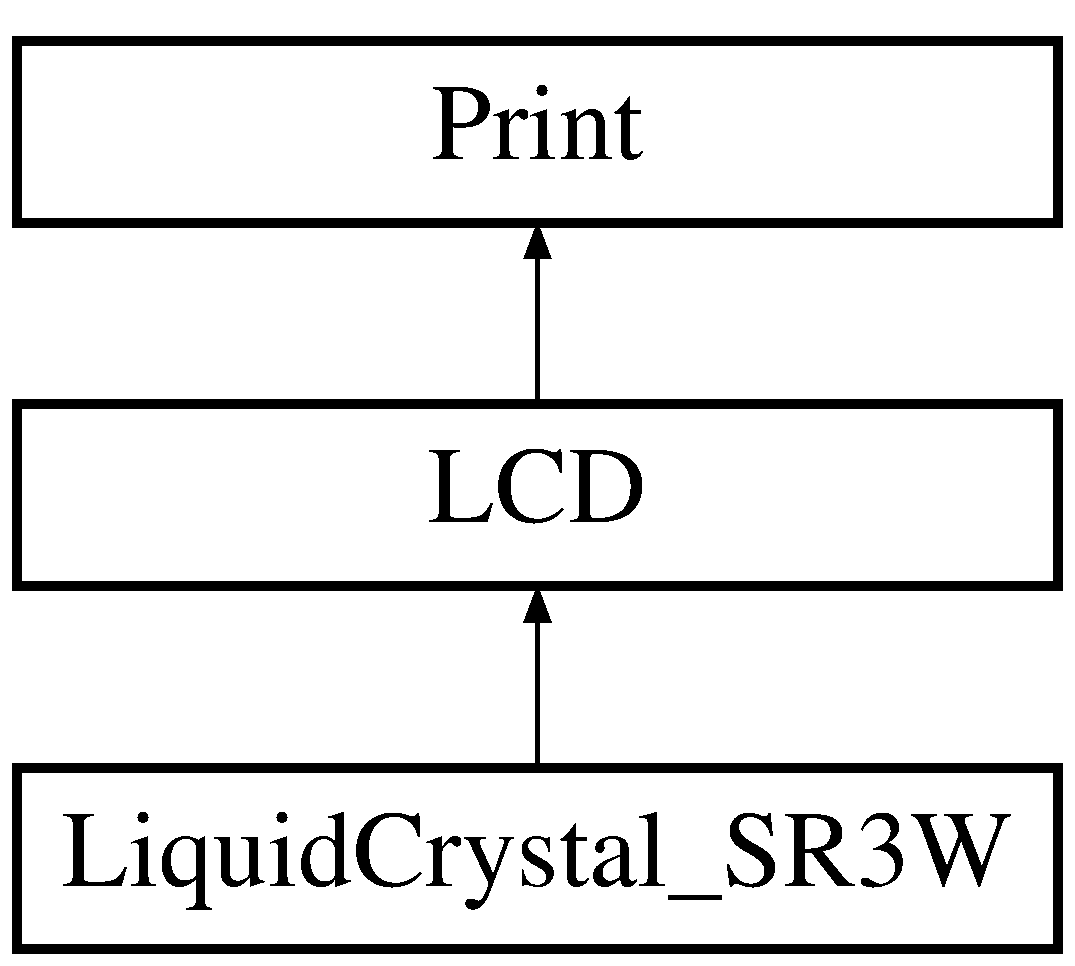
\includegraphics[height=3.000000cm]{class_liquid_crystal___s_r3_w}
\end{center}
\end{figure}
\subsection*{Public Member Functions}
\begin{DoxyCompactItemize}
\item 
\hyperlink{class_liquid_crystal___s_r3_w_ae1396bcd5e9c5b7ed13182c166de776b}{Liquid\+Crystal\+\_\+\+S\+R3\+W} (uint8\+\_\+t data, uint8\+\_\+t clk, uint8\+\_\+t strobe)
\item 
\hypertarget{class_liquid_crystal___s_r3_w_a7b2f382b76bc9d88adb8d681e824b4de}{}{\bfseries Liquid\+Crystal\+\_\+\+S\+R3\+W} (uint8\+\_\+t data, uint8\+\_\+t clk, uint8\+\_\+t strobe, uint8\+\_\+t backligh\+Pin, t\+\_\+backligh\+Pol pol)\label{class_liquid_crystal___s_r3_w_a7b2f382b76bc9d88adb8d681e824b4de}

\item 
\hyperlink{class_liquid_crystal___s_r3_w_a4fab8ff2f21bba3efd133cd8c87fffc0}{Liquid\+Crystal\+\_\+\+S\+R3\+W} (uint8\+\_\+t data, uint8\+\_\+t clk, uint8\+\_\+t strobe, uint8\+\_\+t En, uint8\+\_\+t Rw, uint8\+\_\+t Rs, uint8\+\_\+t d4, uint8\+\_\+t d5, uint8\+\_\+t d6, uint8\+\_\+t d7)
\item 
\hypertarget{class_liquid_crystal___s_r3_w_a24f051747dfeda48f7b207c3358c8015}{}{\bfseries Liquid\+Crystal\+\_\+\+S\+R3\+W} (uint8\+\_\+t data, uint8\+\_\+t clk, uint8\+\_\+t strobe, uint8\+\_\+t En, uint8\+\_\+t Rw, uint8\+\_\+t Rs, uint8\+\_\+t d4, uint8\+\_\+t d5, uint8\+\_\+t d6, uint8\+\_\+t d7, uint8\+\_\+t backligh\+Pin, t\+\_\+backligh\+Pol pol)\label{class_liquid_crystal___s_r3_w_a24f051747dfeda48f7b207c3358c8015}

\item 
virtual void \hyperlink{class_liquid_crystal___s_r3_w_ade34af5b7fe795482f1848c2176d6e56}{send} (uint8\+\_\+t value, uint8\+\_\+t mode)
\item 
void \hyperlink{class_liquid_crystal___s_r3_w_a894d0ea8ea61c1d15acd8a26d417e477}{set\+Backlight\+Pin} (uint8\+\_\+t value, t\+\_\+backligh\+Pol pol)
\item 
void \hyperlink{class_liquid_crystal___s_r3_w_a6d0fc7907ef9fd87c408a21b9bd49295}{set\+Backlight} (uint8\+\_\+t value)
\end{DoxyCompactItemize}
\subsection*{Additional Inherited Members}


\subsection{Constructor \& Destructor Documentation}
\hypertarget{class_liquid_crystal___s_r3_w_ae1396bcd5e9c5b7ed13182c166de776b}{}\index{Liquid\+Crystal\+\_\+\+S\+R3\+W@{Liquid\+Crystal\+\_\+\+S\+R3\+W}!Liquid\+Crystal\+\_\+\+S\+R3\+W@{Liquid\+Crystal\+\_\+\+S\+R3\+W}}
\index{Liquid\+Crystal\+\_\+\+S\+R3\+W@{Liquid\+Crystal\+\_\+\+S\+R3\+W}!Liquid\+Crystal\+\_\+\+S\+R3\+W@{Liquid\+Crystal\+\_\+\+S\+R3\+W}}
\subsubsection[{Liquid\+Crystal\+\_\+\+S\+R3\+W}]{\setlength{\rightskip}{0pt plus 5cm}Liquid\+Crystal\+\_\+\+S\+R3\+W\+::\+Liquid\+Crystal\+\_\+\+S\+R3\+W (
\begin{DoxyParamCaption}
\item[{uint8\+\_\+t}]{data, }
\item[{uint8\+\_\+t}]{clk, }
\item[{uint8\+\_\+t}]{strobe}
\end{DoxyParamCaption}
)}\label{class_liquid_crystal___s_r3_w_ae1396bcd5e9c5b7ed13182c166de776b}
Class constructor.  Initializes class variables and defines the I\+O driving the shift register. The constructor does not initialize the \hyperlink{class_l_c_d}{L\+C\+D}. Default configuration\+: Shift register \hyperlink{class_l_c_d}{L\+C\+D} Q\+A -\/ 0 D\+B4 Q\+B -\/ 1 D\+B5 Q\+C -\/ 2 D\+B6 Q\+D -\/ 3 D\+B7 Q\+E -\/ 4 E Q\+F -\/ 5 Q\+G -\/ 6 Rs G\+N\+D Rw


\begin{DoxyParams}{Parameters}
{\em strobe\mbox{[}in\mbox{]}} & digital I\+O connected to shiftregister strobe pin. \\
\hline
{\em data\mbox{[}in\mbox{]}} & digital I\+O connected to the shiftregister data pin. \\
\hline
{\em clk\mbox{[}in\mbox{]}} & digital I\+O connected to the shiftregister clock pin. \\
\hline
\end{DoxyParams}
\hypertarget{class_liquid_crystal___s_r3_w_a4fab8ff2f21bba3efd133cd8c87fffc0}{}\index{Liquid\+Crystal\+\_\+\+S\+R3\+W@{Liquid\+Crystal\+\_\+\+S\+R3\+W}!Liquid\+Crystal\+\_\+\+S\+R3\+W@{Liquid\+Crystal\+\_\+\+S\+R3\+W}}
\index{Liquid\+Crystal\+\_\+\+S\+R3\+W@{Liquid\+Crystal\+\_\+\+S\+R3\+W}!Liquid\+Crystal\+\_\+\+S\+R3\+W@{Liquid\+Crystal\+\_\+\+S\+R3\+W}}
\subsubsection[{Liquid\+Crystal\+\_\+\+S\+R3\+W}]{\setlength{\rightskip}{0pt plus 5cm}Liquid\+Crystal\+\_\+\+S\+R3\+W\+::\+Liquid\+Crystal\+\_\+\+S\+R3\+W (
\begin{DoxyParamCaption}
\item[{uint8\+\_\+t}]{data, }
\item[{uint8\+\_\+t}]{clk, }
\item[{uint8\+\_\+t}]{strobe, }
\item[{uint8\+\_\+t}]{En, }
\item[{uint8\+\_\+t}]{Rw, }
\item[{uint8\+\_\+t}]{Rs, }
\item[{uint8\+\_\+t}]{d4, }
\item[{uint8\+\_\+t}]{d5, }
\item[{uint8\+\_\+t}]{d6, }
\item[{uint8\+\_\+t}]{d7}
\end{DoxyParamCaption}
)}\label{class_liquid_crystal___s_r3_w_a4fab8ff2f21bba3efd133cd8c87fffc0}
Class constructor.  Initializes class variables and defines the control lines of the \hyperlink{class_l_c_d}{L\+C\+D} and the shiftregister. The constructor does not initialize the \hyperlink{class_l_c_d}{L\+C\+D}.


\begin{DoxyParams}{Parameters}
{\em strobe\mbox{[}in\mbox{]}} & digital I\+O connected to shiftregister strobe pin. \\
\hline
{\em data\mbox{[}in\mbox{]}} & digital I\+O connected to shiftregister data pin. \\
\hline
{\em clk\mbox{[}in\mbox{]}} & digital I\+O connected to shiftregister clock pin. \\
\hline
{\em En\mbox{[}in\mbox{]}} & \hyperlink{class_l_c_d}{L\+C\+D} En (Enable) pin connected to S\+R output pin. \\
\hline
{\em Rw\mbox{[}in\mbox{]}} & \hyperlink{class_l_c_d}{L\+C\+D} Rw (Read/write) pin connected to S\+R output pin. \\
\hline
{\em Rs\mbox{[}in\mbox{]}} & \hyperlink{class_l_c_d}{L\+C\+D} Rs (Reg Select) pin connected to S\+R output pin. \\
\hline
{\em d4\mbox{[}in\mbox{]}} & \hyperlink{class_l_c_d}{L\+C\+D} data 4 pin map to the S\+R output pin. \\
\hline
{\em d5\mbox{[}in\mbox{]}} & \hyperlink{class_l_c_d}{L\+C\+D} data 5 pin map to the S\+R output pin. \\
\hline
{\em d6\mbox{[}in\mbox{]}} & \hyperlink{class_l_c_d}{L\+C\+D} data 6 pin map to the S\+R output pin. \\
\hline
{\em d7\mbox{[}in\mbox{]}} & \hyperlink{class_l_c_d}{L\+C\+D} data 7 pin map to the S\+R output pin. \\
\hline
\end{DoxyParams}


\subsection{Member Function Documentation}
\hypertarget{class_liquid_crystal___s_r3_w_ade34af5b7fe795482f1848c2176d6e56}{}\index{Liquid\+Crystal\+\_\+\+S\+R3\+W@{Liquid\+Crystal\+\_\+\+S\+R3\+W}!send@{send}}
\index{send@{send}!Liquid\+Crystal\+\_\+\+S\+R3\+W@{Liquid\+Crystal\+\_\+\+S\+R3\+W}}
\subsubsection[{send}]{\setlength{\rightskip}{0pt plus 5cm}void Liquid\+Crystal\+\_\+\+S\+R3\+W\+::send (
\begin{DoxyParamCaption}
\item[{uint8\+\_\+t}]{value, }
\item[{uint8\+\_\+t}]{mode}
\end{DoxyParamCaption}
)\hspace{0.3cm}{\ttfamily [virtual]}}\label{class_liquid_crystal___s_r3_w_ade34af5b7fe795482f1848c2176d6e56}
Send a particular value to the \hyperlink{class_l_c_d}{L\+C\+D}.  Sends a particular value to the \hyperlink{class_l_c_d}{L\+C\+D} for writing to the \hyperlink{class_l_c_d}{L\+C\+D} or as an \hyperlink{class_l_c_d}{L\+C\+D} command.

Users should never call this method.


\begin{DoxyParams}{Parameters}
{\em value\mbox{[}in\mbox{]}} & Value to send to the \hyperlink{class_l_c_d}{L\+C\+D}. \\
\hline
{\em mode\mbox{[}in\mbox{]}} & D\+A\+T\+A -\/ write to the \hyperlink{class_l_c_d}{L\+C\+D} C\+G\+R\+A\+M, C\+O\+M\+M\+A\+N\+D -\/ write a command to the \hyperlink{class_l_c_d}{L\+C\+D}. \\
\hline
\end{DoxyParams}


Reimplemented from \hyperlink{class_l_c_d}{L\+C\+D}.

\hypertarget{class_liquid_crystal___s_r3_w_a6d0fc7907ef9fd87c408a21b9bd49295}{}\index{Liquid\+Crystal\+\_\+\+S\+R3\+W@{Liquid\+Crystal\+\_\+\+S\+R3\+W}!set\+Backlight@{set\+Backlight}}
\index{set\+Backlight@{set\+Backlight}!Liquid\+Crystal\+\_\+\+S\+R3\+W@{Liquid\+Crystal\+\_\+\+S\+R3\+W}}
\subsubsection[{set\+Backlight}]{\setlength{\rightskip}{0pt plus 5cm}void Liquid\+Crystal\+\_\+\+S\+R3\+W\+::set\+Backlight (
\begin{DoxyParamCaption}
\item[{uint8\+\_\+t}]{value}
\end{DoxyParamCaption}
)\hspace{0.3cm}{\ttfamily [virtual]}}\label{class_liquid_crystal___s_r3_w_a6d0fc7907ef9fd87c408a21b9bd49295}
Switch-\/on/off the \hyperlink{class_l_c_d}{L\+C\+D} backlight.  Switch-\/on/off the \hyperlink{class_l_c_d}{L\+C\+D} backlight. The set\+Backlight\+Pin has to be called before setting the backlight for this method to work. \begin{DoxySeeAlso}{See also}
\hyperlink{class_liquid_crystal___s_r3_w_a894d0ea8ea61c1d15acd8a26d417e477}{set\+Backlight\+Pin}.
\end{DoxySeeAlso}

\begin{DoxyParams}{Parameters}
{\em value} & backlight mode (H\+I\+G\+H$\vert$\+L\+O\+W) \\
\hline
\end{DoxyParams}


Reimplemented from \hyperlink{class_l_c_d_a3305570d7b37eb93f2cf840263c15828}{L\+C\+D}.

\hypertarget{class_liquid_crystal___s_r3_w_a894d0ea8ea61c1d15acd8a26d417e477}{}\index{Liquid\+Crystal\+\_\+\+S\+R3\+W@{Liquid\+Crystal\+\_\+\+S\+R3\+W}!set\+Backlight\+Pin@{set\+Backlight\+Pin}}
\index{set\+Backlight\+Pin@{set\+Backlight\+Pin}!Liquid\+Crystal\+\_\+\+S\+R3\+W@{Liquid\+Crystal\+\_\+\+S\+R3\+W}}
\subsubsection[{set\+Backlight\+Pin}]{\setlength{\rightskip}{0pt plus 5cm}void Liquid\+Crystal\+\_\+\+S\+R3\+W\+::set\+Backlight\+Pin (
\begin{DoxyParamCaption}
\item[{uint8\+\_\+t}]{value, }
\item[{t\+\_\+backligh\+Pol}]{pol = {\ttfamily POSITIVE}}
\end{DoxyParamCaption}
)\hspace{0.3cm}{\ttfamily [virtual]}}\label{class_liquid_crystal___s_r3_w_a894d0ea8ea61c1d15acd8a26d417e477}
Sets the pin to control the backlight.  Sets the pin in the device to control the backlight. This device doesn\textquotesingle{}t support dimming backlight capability.


\begin{DoxyParams}{Parameters}
{\em 0} & backlight off, 1..255\+: backlight on. \\
\hline
\end{DoxyParams}


Reimplemented from \hyperlink{class_l_c_d_a53f4ee9b39d9ab3d7ae4d9f8dedca3bc}{L\+C\+D}.



The documentation for this class was generated from the following files\+:\begin{DoxyCompactItemize}
\item 
Libraries/\+Liquid\+Crystal/Liquid\+Crystal\+\_\+\+S\+R3\+W.\+h\item 
Libraries/\+Liquid\+Crystal/Liquid\+Crystal\+\_\+\+S\+R3\+W.\+cpp\end{DoxyCompactItemize}

\hypertarget{class_arduino_json_1_1_internals_1_1_list}{}\section{Arduino\+Json\+:\+:Internals\+:\+:List$<$ T $>$ Class Template Reference}
\label{class_arduino_json_1_1_internals_1_1_list}\index{Arduino\+Json\+::\+Internals\+::\+List$<$ T $>$@{Arduino\+Json\+::\+Internals\+::\+List$<$ T $>$}}
\subsection*{Public Types}
\begin{DoxyCompactItemize}
\item 
\hypertarget{class_arduino_json_1_1_internals_1_1_list_a9629d1339871e0c62b620cff9936648d}{}typedef T {\bfseries value\+\_\+type}\label{class_arduino_json_1_1_internals_1_1_list_a9629d1339871e0c62b620cff9936648d}

\item 
\hypertarget{class_arduino_json_1_1_internals_1_1_list_a3bdd86651c7dae3d324a79e73bd35809}{}typedef \hyperlink{struct_arduino_json_1_1_internals_1_1_list_node}{List\+Node}$<$ T $>$ {\bfseries node\+\_\+type}\label{class_arduino_json_1_1_internals_1_1_list_a3bdd86651c7dae3d324a79e73bd35809}

\item 
\hypertarget{class_arduino_json_1_1_internals_1_1_list_afba367ba4c70cf65e53e5dceeaf96e01}{}typedef \hyperlink{class_arduino_json_1_1_internals_1_1_list_iterator}{List\+Iterator}$<$ T $>$ {\bfseries iterator}\label{class_arduino_json_1_1_internals_1_1_list_afba367ba4c70cf65e53e5dceeaf96e01}

\item 
\hypertarget{class_arduino_json_1_1_internals_1_1_list_a647f2c3de1b3810ca31c9041395e83f9}{}typedef \hyperlink{class_arduino_json_1_1_internals_1_1_list_const_iterator}{List\+Const\+Iterator}$<$ T $>$ {\bfseries const\+\_\+iterator}\label{class_arduino_json_1_1_internals_1_1_list_a647f2c3de1b3810ca31c9041395e83f9}

\end{DoxyCompactItemize}
\subsection*{Public Member Functions}
\begin{DoxyCompactItemize}
\item 
\hypertarget{class_arduino_json_1_1_internals_1_1_list_ac80f8ee864f278cc05f23526291a2bca}{}{\bfseries List} (\hyperlink{class_arduino_json_1_1_json_buffer}{Json\+Buffer} $\ast$buffer)\label{class_arduino_json_1_1_internals_1_1_list_ac80f8ee864f278cc05f23526291a2bca}

\item 
\hypertarget{class_arduino_json_1_1_internals_1_1_list_afc78f181d9a4c7974114ce3eaf87d699}{}bool {\bfseries success} () const \label{class_arduino_json_1_1_internals_1_1_list_afc78f181d9a4c7974114ce3eaf87d699}

\item 
\hypertarget{class_arduino_json_1_1_internals_1_1_list_a88f43ce43ec374666d5b990c9af5a823}{}int {\bfseries size} () const \label{class_arduino_json_1_1_internals_1_1_list_a88f43ce43ec374666d5b990c9af5a823}

\item 
\hypertarget{class_arduino_json_1_1_internals_1_1_list_ab682ebbe0064a0f3a9f47c80a0e12281}{}\hyperlink{class_arduino_json_1_1_internals_1_1_list_iterator}{iterator} {\bfseries begin} ()\label{class_arduino_json_1_1_internals_1_1_list_ab682ebbe0064a0f3a9f47c80a0e12281}

\item 
\hypertarget{class_arduino_json_1_1_internals_1_1_list_a413a980b3181a75f9d99f167ca7334ab}{}\hyperlink{class_arduino_json_1_1_internals_1_1_list_iterator}{iterator} {\bfseries end} ()\label{class_arduino_json_1_1_internals_1_1_list_a413a980b3181a75f9d99f167ca7334ab}

\item 
\hypertarget{class_arduino_json_1_1_internals_1_1_list_a19ba4846529160e9136cad0dbb50eb28}{}\hyperlink{class_arduino_json_1_1_internals_1_1_list_const_iterator}{const\+\_\+iterator} {\bfseries begin} () const \label{class_arduino_json_1_1_internals_1_1_list_a19ba4846529160e9136cad0dbb50eb28}

\item 
\hypertarget{class_arduino_json_1_1_internals_1_1_list_ab22cd82cfeb6b1f2ba0faf55de055a76}{}\hyperlink{class_arduino_json_1_1_internals_1_1_list_const_iterator}{const\+\_\+iterator} {\bfseries end} () const \label{class_arduino_json_1_1_internals_1_1_list_ab22cd82cfeb6b1f2ba0faf55de055a76}

\end{DoxyCompactItemize}
\subsection*{Protected Member Functions}
\begin{DoxyCompactItemize}
\item 
\hypertarget{class_arduino_json_1_1_internals_1_1_list_ae6c203678f92189591813b43eff3a2fe}{}\hyperlink{struct_arduino_json_1_1_internals_1_1_list_node}{node\+\_\+type} $\ast$ {\bfseries create\+Node} ()\label{class_arduino_json_1_1_internals_1_1_list_ae6c203678f92189591813b43eff3a2fe}

\item 
\hypertarget{class_arduino_json_1_1_internals_1_1_list_abe0ad43df41d29c3513e86867c3266fe}{}void {\bfseries add\+Node} (\hyperlink{struct_arduino_json_1_1_internals_1_1_list_node}{node\+\_\+type} $\ast$node\+To\+Add)\label{class_arduino_json_1_1_internals_1_1_list_abe0ad43df41d29c3513e86867c3266fe}

\item 
\hypertarget{class_arduino_json_1_1_internals_1_1_list_a05da80e7c1e07d998d9219529edd0e80}{}void {\bfseries remove\+Node} (\hyperlink{struct_arduino_json_1_1_internals_1_1_list_node}{node\+\_\+type} $\ast$node\+To\+Remove)\label{class_arduino_json_1_1_internals_1_1_list_a05da80e7c1e07d998d9219529edd0e80}

\end{DoxyCompactItemize}
\subsection*{Protected Attributes}
\begin{DoxyCompactItemize}
\item 
\hypertarget{class_arduino_json_1_1_internals_1_1_list_a03a87a724dd160debd81d895047c9745}{}\hyperlink{class_arduino_json_1_1_json_buffer}{Json\+Buffer} $\ast$ {\bfseries \+\_\+buffer}\label{class_arduino_json_1_1_internals_1_1_list_a03a87a724dd160debd81d895047c9745}

\item 
\hypertarget{class_arduino_json_1_1_internals_1_1_list_a43e93069e8615279f6c3526fc968f0cf}{}\hyperlink{struct_arduino_json_1_1_internals_1_1_list_node}{node\+\_\+type} $\ast$ {\bfseries \+\_\+first\+Node}\label{class_arduino_json_1_1_internals_1_1_list_a43e93069e8615279f6c3526fc968f0cf}

\end{DoxyCompactItemize}


The documentation for this class was generated from the following files\+:\begin{DoxyCompactItemize}
\item 
Services/\+Arduino\+Json/include/\+Arduino\+Json/\+Internals/List.\+hpp\item 
Services/\+Arduino\+Json/src/\+Internals/List.\+cpp\end{DoxyCompactItemize}

\hypertarget{class_arduino_json_1_1_internals_1_1_list_const_iterator}{}\section{Arduino\+Json\+:\+:Internals\+:\+:List\+Const\+Iterator$<$ T $>$ Class Template Reference}
\label{class_arduino_json_1_1_internals_1_1_list_const_iterator}\index{Arduino\+Json\+::\+Internals\+::\+List\+Const\+Iterator$<$ T $>$@{Arduino\+Json\+::\+Internals\+::\+List\+Const\+Iterator$<$ T $>$}}
\subsection*{Public Member Functions}
\begin{DoxyCompactItemize}
\item 
\hypertarget{class_arduino_json_1_1_internals_1_1_list_const_iterator_ac809f94e5605ba8448e233ac6eb07575}{}{\bfseries List\+Const\+Iterator} (const \hyperlink{struct_arduino_json_1_1_internals_1_1_list_node}{List\+Node}$<$ T $>$ $\ast$node=N\+U\+L\+L)\label{class_arduino_json_1_1_internals_1_1_list_const_iterator_ac809f94e5605ba8448e233ac6eb07575}

\item 
\hypertarget{class_arduino_json_1_1_internals_1_1_list_const_iterator_a8ad8ddbcebb48dc93002eb52213d9035}{}const T \& {\bfseries operator$\ast$} () const \label{class_arduino_json_1_1_internals_1_1_list_const_iterator_a8ad8ddbcebb48dc93002eb52213d9035}

\item 
\hypertarget{class_arduino_json_1_1_internals_1_1_list_const_iterator_a402ffcb21574268972ab1212f377ce85}{}const T $\ast$ {\bfseries operator-\/$>$} ()\label{class_arduino_json_1_1_internals_1_1_list_const_iterator_a402ffcb21574268972ab1212f377ce85}

\item 
\hypertarget{class_arduino_json_1_1_internals_1_1_list_const_iterator_aefeb061c6636cb38fca6dad11bbaa998}{}bool {\bfseries operator==} (const \hyperlink{class_arduino_json_1_1_internals_1_1_list_const_iterator}{List\+Const\+Iterator}$<$ T $>$ \&other) const \label{class_arduino_json_1_1_internals_1_1_list_const_iterator_aefeb061c6636cb38fca6dad11bbaa998}

\item 
\hypertarget{class_arduino_json_1_1_internals_1_1_list_const_iterator_ab5f708a096b6a440d206cebd26df9552}{}bool {\bfseries operator!=} (const \hyperlink{class_arduino_json_1_1_internals_1_1_list_const_iterator}{List\+Const\+Iterator}$<$ T $>$ \&other) const \label{class_arduino_json_1_1_internals_1_1_list_const_iterator_ab5f708a096b6a440d206cebd26df9552}

\item 
\hypertarget{class_arduino_json_1_1_internals_1_1_list_const_iterator_a224941fb91e378484c344012218e946f}{}\hyperlink{class_arduino_json_1_1_internals_1_1_list_const_iterator}{List\+Const\+Iterator}$<$ T $>$ \& {\bfseries operator++} ()\label{class_arduino_json_1_1_internals_1_1_list_const_iterator_a224941fb91e378484c344012218e946f}

\end{DoxyCompactItemize}


The documentation for this class was generated from the following file\+:\begin{DoxyCompactItemize}
\item 
Services/\+Arduino\+Json/include/\+Arduino\+Json/\+Internals/List\+Const\+Iterator.\+hpp\end{DoxyCompactItemize}

\hypertarget{class_arduino_json_1_1_internals_1_1_list_iterator}{}\section{Arduino\+Json\+:\+:Internals\+:\+:List\+Iterator$<$ T $>$ Class Template Reference}
\label{class_arduino_json_1_1_internals_1_1_list_iterator}\index{Arduino\+Json\+::\+Internals\+::\+List\+Iterator$<$ T $>$@{Arduino\+Json\+::\+Internals\+::\+List\+Iterator$<$ T $>$}}
\subsection*{Public Member Functions}
\begin{DoxyCompactItemize}
\item 
\hypertarget{class_arduino_json_1_1_internals_1_1_list_iterator_aa9f2fd9b3be020a40764fc24e2435b0a}{}{\bfseries List\+Iterator} (\hyperlink{struct_arduino_json_1_1_internals_1_1_list_node}{List\+Node}$<$ T $>$ $\ast$node=N\+U\+L\+L)\label{class_arduino_json_1_1_internals_1_1_list_iterator_aa9f2fd9b3be020a40764fc24e2435b0a}

\item 
\hypertarget{class_arduino_json_1_1_internals_1_1_list_iterator_a64252b2b759171d7e9dccd38548a5ea7}{}T \& {\bfseries operator$\ast$} () const \label{class_arduino_json_1_1_internals_1_1_list_iterator_a64252b2b759171d7e9dccd38548a5ea7}

\item 
\hypertarget{class_arduino_json_1_1_internals_1_1_list_iterator_abda1d47194335611e6696f50a82f79a7}{}T $\ast$ {\bfseries operator-\/$>$} ()\label{class_arduino_json_1_1_internals_1_1_list_iterator_abda1d47194335611e6696f50a82f79a7}

\item 
\hypertarget{class_arduino_json_1_1_internals_1_1_list_iterator_af04982ed9940f52b701860b1b4de97cf}{}bool {\bfseries operator==} (const \hyperlink{class_arduino_json_1_1_internals_1_1_list_iterator}{List\+Iterator}$<$ T $>$ \&other) const \label{class_arduino_json_1_1_internals_1_1_list_iterator_af04982ed9940f52b701860b1b4de97cf}

\item 
\hypertarget{class_arduino_json_1_1_internals_1_1_list_iterator_acea1211ac8992c6776c7a34cb0a68573}{}bool {\bfseries operator!=} (const \hyperlink{class_arduino_json_1_1_internals_1_1_list_iterator}{List\+Iterator}$<$ T $>$ \&other) const \label{class_arduino_json_1_1_internals_1_1_list_iterator_acea1211ac8992c6776c7a34cb0a68573}

\item 
\hypertarget{class_arduino_json_1_1_internals_1_1_list_iterator_af60629257f949bdc0371f0c55b948045}{}\hyperlink{class_arduino_json_1_1_internals_1_1_list_iterator}{List\+Iterator}$<$ T $>$ \& {\bfseries operator++} ()\label{class_arduino_json_1_1_internals_1_1_list_iterator_af60629257f949bdc0371f0c55b948045}

\item 
\hypertarget{class_arduino_json_1_1_internals_1_1_list_iterator_a54e20f29652d9d98fe7d848510fe2652}{}{\bfseries operator List\+Const\+Iterator$<$ T $>$} () const \label{class_arduino_json_1_1_internals_1_1_list_iterator_a54e20f29652d9d98fe7d848510fe2652}

\end{DoxyCompactItemize}


The documentation for this class was generated from the following file\+:\begin{DoxyCompactItemize}
\item 
Services/\+Arduino\+Json/include/\+Arduino\+Json/\+Internals/List\+Iterator.\+hpp\end{DoxyCompactItemize}

\hypertarget{struct_arduino_json_1_1_internals_1_1_list_node}{}\section{Arduino\+Json\+:\+:Internals\+:\+:List\+Node$<$ T $>$ Struct Template Reference}
\label{struct_arduino_json_1_1_internals_1_1_list_node}\index{Arduino\+Json\+::\+Internals\+::\+List\+Node$<$ T $>$@{Arduino\+Json\+::\+Internals\+::\+List\+Node$<$ T $>$}}
Inheritance diagram for Arduino\+Json\+:\+:Internals\+:\+:List\+Node$<$ T $>$\+:\begin{figure}[H]
\begin{center}
\leavevmode
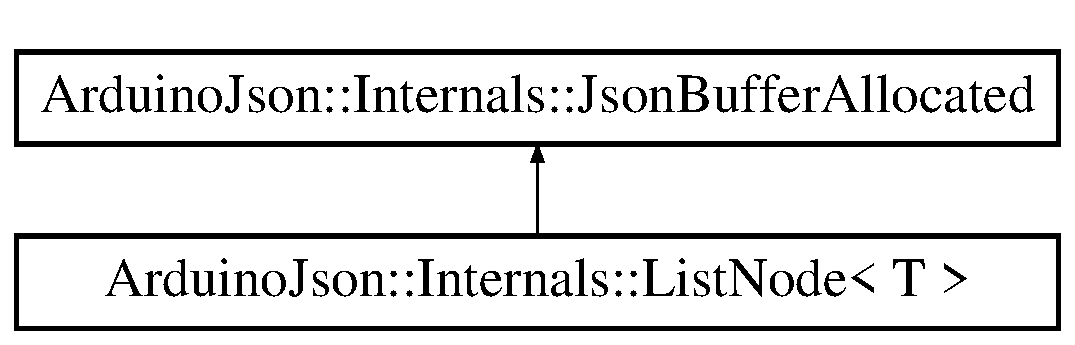
\includegraphics[height=2.000000cm]{struct_arduino_json_1_1_internals_1_1_list_node}
\end{center}
\end{figure}
\subsection*{Public Attributes}
\begin{DoxyCompactItemize}
\item 
\hypertarget{struct_arduino_json_1_1_internals_1_1_list_node_af02682d631b75f87db9e877b7c099b40}{}\hyperlink{struct_arduino_json_1_1_internals_1_1_list_node}{List\+Node}$<$ T $>$ $\ast$ {\bfseries next}\label{struct_arduino_json_1_1_internals_1_1_list_node_af02682d631b75f87db9e877b7c099b40}

\item 
\hypertarget{struct_arduino_json_1_1_internals_1_1_list_node_a959fc0e35711df83d3edd13015c8ee5f}{}T {\bfseries content}\label{struct_arduino_json_1_1_internals_1_1_list_node_a959fc0e35711df83d3edd13015c8ee5f}

\end{DoxyCompactItemize}
\subsection*{Additional Inherited Members}


The documentation for this struct was generated from the following file\+:\begin{DoxyCompactItemize}
\item 
Services/\+Arduino\+Json/include/\+Arduino\+Json/\+Internals/List\+Node.\+hpp\end{DoxyCompactItemize}

\hypertarget{class_memory_data_stream}{}\section{Memory\+Data\+Stream Class Reference}
\label{class_memory_data_stream}\index{Memory\+Data\+Stream@{Memory\+Data\+Stream}}
Inheritance diagram for Memory\+Data\+Stream\+:\begin{figure}[H]
\begin{center}
\leavevmode
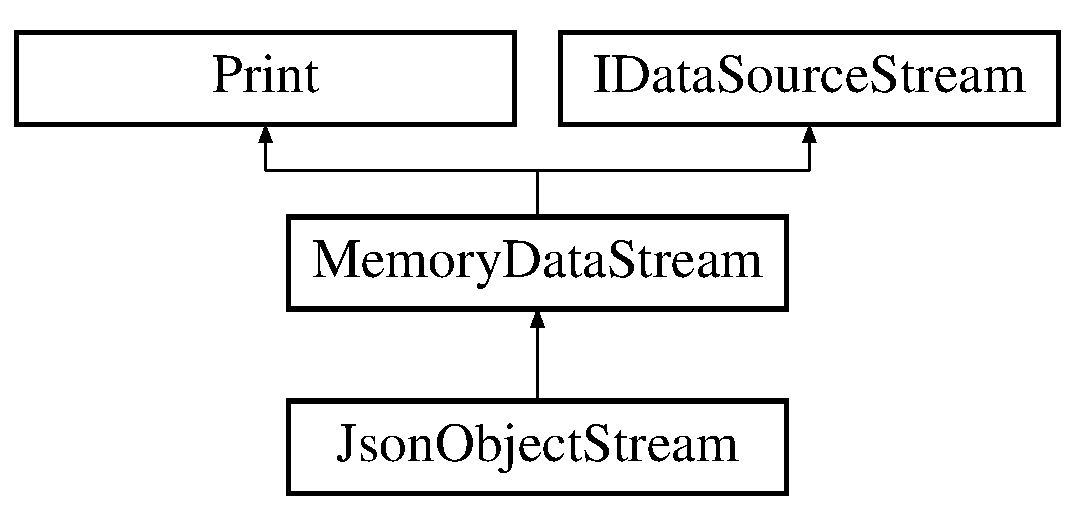
\includegraphics[height=3.000000cm]{class_memory_data_stream}
\end{center}
\end{figure}
\subsection*{Public Member Functions}
\begin{DoxyCompactItemize}
\item 
\hypertarget{class_memory_data_stream_a29d74d448be139ab37649b7170490807}{}virtual Stream\+Type {\bfseries get\+Stream\+Type} ()\label{class_memory_data_stream_a29d74d448be139ab37649b7170490807}

\item 
\hypertarget{class_memory_data_stream_a354c172099a391a98799f5543a1d9976}{}virtual size\+\_\+t {\bfseries write} (uint8\+\_\+t char\+To\+Write)\label{class_memory_data_stream_a354c172099a391a98799f5543a1d9976}

\item 
\hypertarget{class_memory_data_stream_abe83097f3f9edeb5b7712c9c91be65c9}{}virtual size\+\_\+t {\bfseries write} (const uint8\+\_\+t $\ast$buffer, size\+\_\+t size)\label{class_memory_data_stream_abe83097f3f9edeb5b7712c9c91be65c9}

\item 
\hypertarget{class_memory_data_stream_a6453a186b60d014da601f73e1b6b8551}{}virtual uint16\+\_\+t {\bfseries get\+Data\+Pointer} (char $\ast$$\ast$data)\label{class_memory_data_stream_a6453a186b60d014da601f73e1b6b8551}

\item 
\hypertarget{class_memory_data_stream_a0ba5090f3f43b7ba49c2f1f5f744303c}{}virtual bool {\bfseries seek} (int len)\label{class_memory_data_stream_a0ba5090f3f43b7ba49c2f1f5f744303c}

\item 
\hypertarget{class_memory_data_stream_a682a22c988c2131606f22e30bb7263ae}{}virtual bool {\bfseries is\+Finished} ()\label{class_memory_data_stream_a682a22c988c2131606f22e30bb7263ae}

\end{DoxyCompactItemize}


The documentation for this class was generated from the following files\+:\begin{DoxyCompactItemize}
\item 
Sming\+Core/Data\+Source\+Stream.\+h\item 
Sming\+Core/Data\+Source\+Stream.\+cpp\end{DoxyCompactItemize}

\hypertarget{class_method_caller}{}\section{Method\+Caller$<$ class $>$ Class Template Reference}
\label{class_method_caller}\index{Method\+Caller$<$ class $>$@{Method\+Caller$<$ class $>$}}


The documentation for this class was generated from the following file\+:\begin{DoxyCompactItemize}
\item 
Sming\+Core/Delegate.\+h\end{DoxyCompactItemize}

\hypertarget{class_method_caller_3_01_return_type_07_class_type_1_1_5_08_07_params_list_8_8_8_08_4}{}\section{Method\+Caller$<$ Return\+Type(Class\+Type\+:\+:$\ast$)(Params\+List...)$>$ Class Template Reference}
\label{class_method_caller_3_01_return_type_07_class_type_1_1_5_08_07_params_list_8_8_8_08_4}\index{Method\+Caller$<$ Return\+Type(\+Class\+Type\+::$\ast$)(\+Params\+List...)$>$@{Method\+Caller$<$ Return\+Type(\+Class\+Type\+::$\ast$)(\+Params\+List...)$>$}}
Inheritance diagram for Method\+Caller$<$ Return\+Type(Class\+Type\+:\+:$\ast$)(Params\+List...)$>$\+:\begin{figure}[H]
\begin{center}
\leavevmode
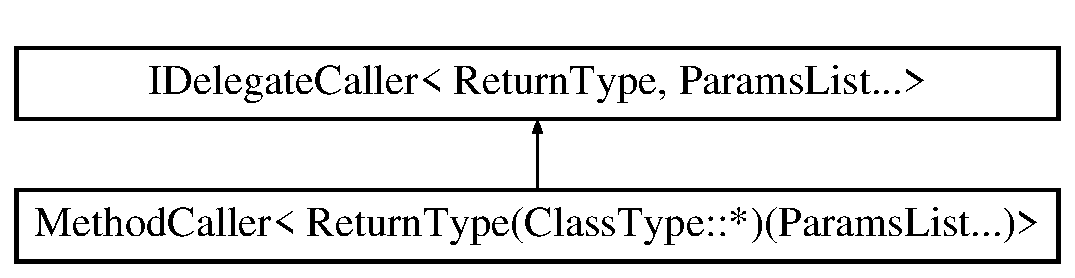
\includegraphics[height=2.000000cm]{class_method_caller_3_01_return_type_07_class_type_1_1_5_08_07_params_list_8_8_8_08_4}
\end{center}
\end{figure}
\subsection*{Public Member Functions}
\begin{DoxyCompactItemize}
\item 
\hypertarget{class_method_caller_3_01_return_type_07_class_type_1_1_5_08_07_params_list_8_8_8_08_4_a1438e54a0922ae6473a48e0183f95c2d}{}{\bfseries Method\+Caller} (Class\+Type $\ast$c, Method\+Declaration m)\label{class_method_caller_3_01_return_type_07_class_type_1_1_5_08_07_params_list_8_8_8_08_4_a1438e54a0922ae6473a48e0183f95c2d}

\item 
\hypertarget{class_method_caller_3_01_return_type_07_class_type_1_1_5_08_07_params_list_8_8_8_08_4_afb12bfdaa1c645537c1d09a6c67e1658}{}Return\+Type {\bfseries invoke} (Params\+List...\+args)\label{class_method_caller_3_01_return_type_07_class_type_1_1_5_08_07_params_list_8_8_8_08_4_afb12bfdaa1c645537c1d09a6c67e1658}

\end{DoxyCompactItemize}


The documentation for this class was generated from the following file\+:\begin{DoxyCompactItemize}
\item 
Sming\+Core/Delegate.\+h\end{DoxyCompactItemize}

\hypertarget{structmqtt__broker__handle__t}{}\section{mqtt\+\_\+broker\+\_\+handle\+\_\+t Struct Reference}
\label{structmqtt__broker__handle__t}\index{mqtt\+\_\+broker\+\_\+handle\+\_\+t@{mqtt\+\_\+broker\+\_\+handle\+\_\+t}}
\subsection*{Public Attributes}
\begin{DoxyCompactItemize}
\item 
\hypertarget{structmqtt__broker__handle__t_a92aed5f346d3407642bf44950727393f}{}void $\ast$ {\bfseries socket\+\_\+info}\label{structmqtt__broker__handle__t_a92aed5f346d3407642bf44950727393f}

\item 
\hypertarget{structmqtt__broker__handle__t_a6ba16eeee3364246f62f48650c2304e9}{}int($\ast$ {\bfseries send} )(void $\ast$socket\+\_\+info, const void $\ast$buf, unsigned int count)\label{structmqtt__broker__handle__t_a6ba16eeee3364246f62f48650c2304e9}

\item 
\hypertarget{structmqtt__broker__handle__t_a5775a5d98521617889eec376cd6e7ef2}{}char {\bfseries clientid} \mbox{[}50\mbox{]}\label{structmqtt__broker__handle__t_a5775a5d98521617889eec376cd6e7ef2}

\item 
\hypertarget{structmqtt__broker__handle__t_a8e3bd673bce26ab301a72ca83850284a}{}char {\bfseries username} \mbox{[}M\+Q\+T\+T\+\_\+\+C\+O\+N\+F\+\_\+\+U\+S\+E\+R\+N\+A\+M\+E\+\_\+\+L\+E\+N\+G\+T\+H\mbox{]}\label{structmqtt__broker__handle__t_a8e3bd673bce26ab301a72ca83850284a}

\item 
\hypertarget{structmqtt__broker__handle__t_ae1d422e8ee6e24a933caf1c5629b7ad9}{}char {\bfseries password} \mbox{[}M\+Q\+T\+T\+\_\+\+C\+O\+N\+F\+\_\+\+P\+A\+S\+S\+W\+O\+R\+D\+\_\+\+L\+E\+N\+G\+T\+H\mbox{]}\label{structmqtt__broker__handle__t_ae1d422e8ee6e24a933caf1c5629b7ad9}

\item 
\hypertarget{structmqtt__broker__handle__t_a8c13600b493f9de4c681e8f613174e26}{}uint8\+\_\+t {\bfseries will\+\_\+retain}\label{structmqtt__broker__handle__t_a8c13600b493f9de4c681e8f613174e26}

\item 
\hypertarget{structmqtt__broker__handle__t_a9e072b6ccb3d43b3900915b4a7a6de5b}{}uint8\+\_\+t {\bfseries will\+\_\+qos}\label{structmqtt__broker__handle__t_a9e072b6ccb3d43b3900915b4a7a6de5b}

\item 
\hypertarget{structmqtt__broker__handle__t_abe6a10fec995a17c758f57a47fdec3df}{}uint8\+\_\+t {\bfseries clean\+\_\+session}\label{structmqtt__broker__handle__t_abe6a10fec995a17c758f57a47fdec3df}

\item 
\hypertarget{structmqtt__broker__handle__t_adb7402c8cdef8cd741361db4408c4a7f}{}uint16\+\_\+t {\bfseries seq}\label{structmqtt__broker__handle__t_adb7402c8cdef8cd741361db4408c4a7f}

\item 
\hypertarget{structmqtt__broker__handle__t_a9ab69668005e780ba5d967f9407a1226}{}uint16\+\_\+t {\bfseries alive}\label{structmqtt__broker__handle__t_a9ab69668005e780ba5d967f9407a1226}

\end{DoxyCompactItemize}


The documentation for this struct was generated from the following file\+:\begin{DoxyCompactItemize}
\item 
Services/libemqtt/libemqtt.\+h\end{DoxyCompactItemize}

\hypertarget{class_mqtt_client}{}\section{Mqtt\+Client Class Reference}
\label{class_mqtt_client}\index{Mqtt\+Client@{Mqtt\+Client}}
Inheritance diagram for Mqtt\+Client\+:\begin{figure}[H]
\begin{center}
\leavevmode
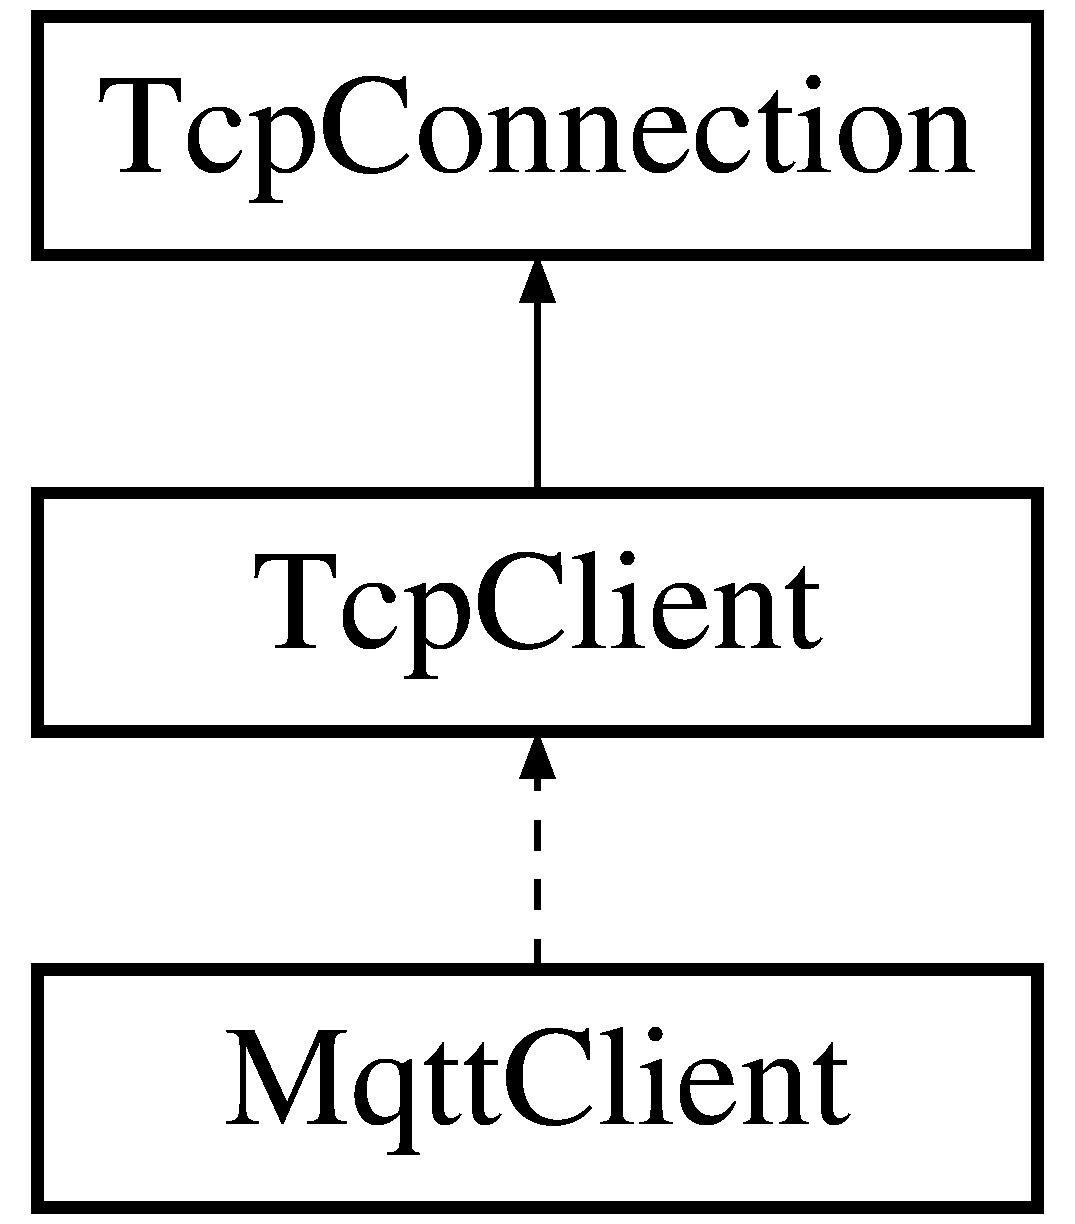
\includegraphics[height=3.000000cm]{class_mqtt_client}
\end{center}
\end{figure}
\subsection*{Public Member Functions}
\begin{DoxyCompactItemize}
\item 
\hypertarget{class_mqtt_client_ae81fd0caf267d95579f2b17689a94b9d}{}{\bfseries Mqtt\+Client} (String server\+Host, int server\+Port, \hyperlink{class_delegate}{Mqtt\+String\+Subscription\+Callback} callback=N\+U\+L\+L)\label{class_mqtt_client_ae81fd0caf267d95579f2b17689a94b9d}

\item 
\hypertarget{class_mqtt_client_a5254838ca1080dea6678ab1502381865}{}bool {\bfseries connect} (String client\+Name)\label{class_mqtt_client_a5254838ca1080dea6678ab1502381865}

\item 
\hypertarget{class_mqtt_client_a155b0c0aa5b18eb99d9cac49e7537d64}{}bool {\bfseries connect} (String client\+Name, String username, String password)\label{class_mqtt_client_a155b0c0aa5b18eb99d9cac49e7537d64}

\item 
\hypertarget{class_mqtt_client_ae79eaa6ffbd4b60073660f19372bb231}{}\+\_\+\+\_\+forceinline bool {\bfseries is\+Processing} ()\label{class_mqtt_client_ae79eaa6ffbd4b60073660f19372bb231}

\item 
\hypertarget{class_mqtt_client_ab9ec80e0dc68f1b5876d6bc0907c0649}{}\+\_\+\+\_\+forceinline Tcp\+Client\+State {\bfseries get\+State} ()\label{class_mqtt_client_ab9ec80e0dc68f1b5876d6bc0907c0649}

\item 
\hypertarget{class_mqtt_client_a8e2571378d6466093b36d411472d0e75}{}bool {\bfseries publish} (String topic, String message, bool retained=false)\label{class_mqtt_client_a8e2571378d6466093b36d411472d0e75}

\item 
\hypertarget{class_mqtt_client_a522c102c900fc19939c3995162abb56f}{}bool {\bfseries publish\+With\+Qo\+S} (String topic, String message, int Qo\+S, bool retained=false)\label{class_mqtt_client_a522c102c900fc19939c3995162abb56f}

\item 
\hypertarget{class_mqtt_client_ad3b2e16ea29d7171fe8afc727b2964f5}{}bool {\bfseries subscribe} (String topic)\label{class_mqtt_client_ad3b2e16ea29d7171fe8afc727b2964f5}

\item 
\hypertarget{class_mqtt_client_a648ef9e9a4d2858b08a2d378da105f96}{}bool {\bfseries unsubscribe} (String topic)\label{class_mqtt_client_a648ef9e9a4d2858b08a2d378da105f96}

\end{DoxyCompactItemize}
\subsection*{Protected Member Functions}
\begin{DoxyCompactItemize}
\item 
\hypertarget{class_mqtt_client_a64d332ee4caddc73030f4bc5f26cd60f}{}virtual err\+\_\+t {\bfseries on\+Receive} (\hyperlink{structpbuf}{pbuf} $\ast$buf)\label{class_mqtt_client_a64d332ee4caddc73030f4bc5f26cd60f}

\item 
\hypertarget{class_mqtt_client_ad9f0e46e11d19c0f766242d20048c70c}{}virtual void {\bfseries on\+Ready\+To\+Send\+Data} (Tcp\+Connection\+Event source\+Event)\label{class_mqtt_client_ad9f0e46e11d19c0f766242d20048c70c}

\item 
\hypertarget{class_mqtt_client_a6a515cf9e00ae813a7dbfa172a081db6}{}void {\bfseries debug\+Print\+Response\+Type} (int type, int len)\label{class_mqtt_client_a6a515cf9e00ae813a7dbfa172a081db6}

\end{DoxyCompactItemize}
\subsection*{Static Protected Member Functions}
\begin{DoxyCompactItemize}
\item 
\hypertarget{class_mqtt_client_ac6bf0f650f5b29708bce6b10235806aa}{}static int {\bfseries static\+Send\+Packet} (void $\ast$user\+Info, const void $\ast$buf, unsigned int count)\label{class_mqtt_client_ac6bf0f650f5b29708bce6b10235806aa}

\end{DoxyCompactItemize}
\subsection*{Additional Inherited Members}


The documentation for this class was generated from the following files\+:\begin{DoxyCompactItemize}
\item 
Sming\+Core/\+Network/Mqtt\+Client.\+h\item 
Sming\+Core/\+Network/Mqtt\+Client.\+cpp\end{DoxyCompactItemize}

\hypertarget{structnetbuf}{}\section{netbuf Struct Reference}
\label{structnetbuf}\index{netbuf@{netbuf}}
\subsection*{Public Attributes}
\begin{DoxyCompactItemize}
\item 
\hypertarget{structnetbuf_ae0c3ba45f7e26a90585c8d79d59c41bd}{}struct \hyperlink{structpbuf}{pbuf} $\ast$ {\bfseries p}\label{structnetbuf_ae0c3ba45f7e26a90585c8d79d59c41bd}

\item 
\hypertarget{structnetbuf_a2301ad2b03edfb74049a2b0ef6cd2cd5}{}struct \hyperlink{structpbuf}{pbuf} $\ast$ {\bfseries ptr}\label{structnetbuf_a2301ad2b03edfb74049a2b0ef6cd2cd5}

\item 
\hypertarget{structnetbuf_a36d0b956d15d9eea205055e227143856}{}ip\+\_\+addr\+\_\+t {\bfseries addr}\label{structnetbuf_a36d0b956d15d9eea205055e227143856}

\item 
\hypertarget{structnetbuf_ac7a45470930d48463b039af4bf464fc4}{}u16\+\_\+t {\bfseries port}\label{structnetbuf_ac7a45470930d48463b039af4bf464fc4}

\end{DoxyCompactItemize}


The documentation for this struct was generated from the following file\+:\begin{DoxyCompactItemize}
\item 
system/include/lwip/netbuf.\+h\end{DoxyCompactItemize}

\hypertarget{structnetif}{}\section{netif Struct Reference}
\label{structnetif}\index{netif@{netif}}


{\ttfamily \#include $<$netif.\+h$>$}

\subsection*{Public Attributes}
\begin{DoxyCompactItemize}
\item 
struct \hyperlink{structnetif}{netif} $\ast$ \hyperlink{structnetif_ae77736b64df442242795220d76be6b86}{next}
\item 
ip\+\_\+addr\+\_\+t \hyperlink{structnetif_a9776aaee37ea8f07b9ddc0f8b4e7e866}{ip\+\_\+addr}
\item 
\hypertarget{structnetif_a5192f2fa2533f13cfde07d9d5bb0db2b}{}ip\+\_\+addr\+\_\+t {\bfseries netmask}\label{structnetif_a5192f2fa2533f13cfde07d9d5bb0db2b}

\item 
\hypertarget{structnetif_a353875b68ea303d237d1c3406134ec76}{}ip\+\_\+addr\+\_\+t {\bfseries gw}\label{structnetif_a353875b68ea303d237d1c3406134ec76}

\item 
netif\+\_\+input\+\_\+fn \hyperlink{structnetif_a8fe4f1b7b0d710216287da9615164a5c}{input}
\item 
netif\+\_\+output\+\_\+fn \hyperlink{structnetif_a8e1dcfe65db487feecd244355f39215e}{output}
\item 
netif\+\_\+linkoutput\+\_\+fn \hyperlink{structnetif_acaaac9b415a7be73eb8a287c8ed18a8d}{linkoutput}
\item 
void $\ast$ \hyperlink{structnetif_a809cc57c0dff09c5c9ae45b02c2002f3}{state}
\item 
u16\+\_\+t \hyperlink{structnetif_aca7d56b4e0f822b0ced2885f222b8d48}{mtu}
\item 
u8\+\_\+t \hyperlink{structnetif_afe1181561cb16241f3cb5ed01e567d42}{hwaddr\+\_\+len}
\item 
u8\+\_\+t \hyperlink{structnetif_ab91f76223d5a7f1a64f03ac9dd7113a4}{hwaddr} \mbox{[}N\+E\+T\+I\+F\+\_\+\+M\+A\+X\+\_\+\+H\+W\+A\+D\+D\+R\+\_\+\+L\+E\+N\mbox{]}
\item 
u8\+\_\+t \hyperlink{structnetif_a1c171db6097bbb6f09f63549a66e00ea}{flags}
\item 
char \hyperlink{structnetif_a32fca6ffd28bb9af3f891a378827a67e}{name} \mbox{[}2\mbox{]}
\item 
u8\+\_\+t \hyperlink{structnetif_ab7ef01e505dd2feb781fe86756b1c973}{num}
\end{DoxyCompactItemize}


\subsection{Detailed Description}
Generic data structure used for all lw\+I\+P network interfaces. The following fields should be filled in by the initialization function for the device driver\+: hwaddr\+\_\+len, hwaddr\mbox{[}\mbox{]}, mtu, flags 

\subsection{Member Data Documentation}
\hypertarget{structnetif_a1c171db6097bbb6f09f63549a66e00ea}{}\index{netif@{netif}!flags@{flags}}
\index{flags@{flags}!netif@{netif}}
\subsubsection[{flags}]{\setlength{\rightskip}{0pt plus 5cm}u8\+\_\+t netif\+::flags}\label{structnetif_a1c171db6097bbb6f09f63549a66e00ea}
flags (see N\+E\+T\+I\+F\+\_\+\+F\+L\+A\+G\+\_\+ above) �ýӿ�״̬�������ֶ� \hypertarget{structnetif_ab91f76223d5a7f1a64f03ac9dd7113a4}{}\index{netif@{netif}!hwaddr@{hwaddr}}
\index{hwaddr@{hwaddr}!netif@{netif}}
\subsubsection[{hwaddr}]{\setlength{\rightskip}{0pt plus 5cm}u8\+\_\+t netif\+::hwaddr\mbox{[}N\+E\+T\+I\+F\+\_\+\+M\+A\+X\+\_\+\+H\+W\+A\+D\+D\+R\+\_\+\+L\+E\+N\mbox{]}}\label{structnetif_ab91f76223d5a7f1a64f03ac9dd7113a4}
link level hardware address of this interface �ýӿ�������ַ \hypertarget{structnetif_afe1181561cb16241f3cb5ed01e567d42}{}\index{netif@{netif}!hwaddr\+\_\+len@{hwaddr\+\_\+len}}
\index{hwaddr\+\_\+len@{hwaddr\+\_\+len}!netif@{netif}}
\subsubsection[{hwaddr\+\_\+len}]{\setlength{\rightskip}{0pt plus 5cm}u8\+\_\+t netif\+::hwaddr\+\_\+len}\label{structnetif_afe1181561cb16241f3cb5ed01e567d42}
number of bytes used in hwaddr�ýӿ�������ַ���� \hypertarget{structnetif_a8fe4f1b7b0d710216287da9615164a5c}{}\index{netif@{netif}!input@{input}}
\index{input@{input}!netif@{netif}}
\subsubsection[{input}]{\setlength{\rightskip}{0pt plus 5cm}netif\+\_\+input\+\_\+fn netif\+::input}\label{structnetif_a8fe4f1b7b0d710216287da9615164a5c}
This function is called by the network device driver to pass a packet up the T\+C\+P/\+I\+P stack. ��\+I\+P���������ݰ� \hypertarget{structnetif_a9776aaee37ea8f07b9ddc0f8b4e7e866}{}\index{netif@{netif}!ip\+\_\+addr@{ip\+\_\+addr}}
\index{ip\+\_\+addr@{ip\+\_\+addr}!netif@{netif}}
\subsubsection[{ip\+\_\+addr}]{\setlength{\rightskip}{0pt plus 5cm}ip\+\_\+addr\+\_\+t netif\+::ip\+\_\+addr}\label{structnetif_a9776aaee37ea8f07b9ddc0f8b4e7e866}
I\+P address configuration in network byte order \hypertarget{structnetif_acaaac9b415a7be73eb8a287c8ed18a8d}{}\index{netif@{netif}!linkoutput@{linkoutput}}
\index{linkoutput@{linkoutput}!netif@{netif}}
\subsubsection[{linkoutput}]{\setlength{\rightskip}{0pt plus 5cm}netif\+\_\+linkoutput\+\_\+fn netif\+::linkoutput}\label{structnetif_acaaac9b415a7be73eb8a287c8ed18a8d}
This function is called by the A\+R\+P module when it wants to send a packet on the interface. This function outputs the pbuf as-\/is on the link medium. �ײ����ݰ����� \hypertarget{structnetif_aca7d56b4e0f822b0ced2885f222b8d48}{}\index{netif@{netif}!mtu@{mtu}}
\index{mtu@{mtu}!netif@{netif}}
\subsubsection[{mtu}]{\setlength{\rightskip}{0pt plus 5cm}u16\+\_\+t netif\+::mtu}\label{structnetif_aca7d56b4e0f822b0ced2885f222b8d48}
maximum transfer unit (in bytes) �ýӿ�������������ݰ����ȣ�����1500 \hypertarget{structnetif_a32fca6ffd28bb9af3f891a378827a67e}{}\index{netif@{netif}!name@{name}}
\index{name@{name}!netif@{netif}}
\subsubsection[{name}]{\setlength{\rightskip}{0pt plus 5cm}char netif\+::name\mbox{[}2\mbox{]}}\label{structnetif_a32fca6ffd28bb9af3f891a378827a67e}
descriptive abbreviation �ýӿڵ����� \hypertarget{structnetif_ae77736b64df442242795220d76be6b86}{}\index{netif@{netif}!next@{next}}
\index{next@{next}!netif@{netif}}
\subsubsection[{next}]{\setlength{\rightskip}{0pt plus 5cm}struct {\bf netif}$\ast$ netif\+::next}\label{structnetif_ae77736b64df442242795220d76be6b86}
pointer to next in linked list \hypertarget{structnetif_ab7ef01e505dd2feb781fe86756b1c973}{}\index{netif@{netif}!num@{num}}
\index{num@{num}!netif@{netif}}
\subsubsection[{num}]{\setlength{\rightskip}{0pt plus 5cm}u8\+\_\+t netif\+::num}\label{structnetif_ab7ef01e505dd2feb781fe86756b1c973}
number of this interface �ýӿڵı�� \hypertarget{structnetif_a8e1dcfe65db487feecd244355f39215e}{}\index{netif@{netif}!output@{output}}
\index{output@{output}!netif@{netif}}
\subsubsection[{output}]{\setlength{\rightskip}{0pt plus 5cm}netif\+\_\+output\+\_\+fn netif\+::output}\label{structnetif_a8e1dcfe65db487feecd244355f39215e}
This function is called by the I\+P module when it wants to send a packet on the interface. This function typically first resolves the hardware address, then sends the packet. ����\+I\+P���ݰ� \hypertarget{structnetif_a809cc57c0dff09c5c9ae45b02c2002f3}{}\index{netif@{netif}!state@{state}}
\index{state@{state}!netif@{netif}}
\subsubsection[{state}]{\setlength{\rightskip}{0pt plus 5cm}void$\ast$ netif\+::state}\label{structnetif_a809cc57c0dff09c5c9ae45b02c2002f3}
This field can be set by the device driver and could point to state information for the device. ���������ֶΣ�����ָ��ײ��豸�����Ϣ 

The documentation for this struct was generated from the following file\+:\begin{DoxyCompactItemize}
\item 
system/include/lwip/netif.\+h\end{DoxyCompactItemize}

\hypertarget{class_net_utils}{}\section{Net\+Utils Class Reference}
\label{class_net_utils}\index{Net\+Utils@{Net\+Utils}}
\subsection*{Public Member Functions}
\begin{DoxyCompactItemize}
\item 
\hypertarget{class_net_utils_ab1f132b29ac270fc1a699cc21a4448b2}{}void {\bfseries debug\+Print\+Tcp\+List} ()\label{class_net_utils_ab1f132b29ac270fc1a699cc21a4448b2}

\end{DoxyCompactItemize}
\subsection*{Static Public Member Functions}
\begin{DoxyCompactItemize}
\item 
\hypertarget{class_net_utils_a8d5f716027c7f9fe588058a5f7382c18}{}static bool {\bfseries pbuf\+Is\+Str\+Equal} (\hyperlink{structpbuf}{pbuf} $\ast$buf, const char $\ast$compared, int start\+Pos)\label{class_net_utils_a8d5f716027c7f9fe588058a5f7382c18}

\item 
\hypertarget{class_net_utils_a0b0353dfd9aeae9b1f16275db7699168}{}static int \hyperlink{class_net_utils_a0b0353dfd9aeae9b1f16275db7699168}{pbuf\+Find\+Char} (\hyperlink{structpbuf}{pbuf} $\ast$buf, char wtf, int start\+Pos=0)\label{class_net_utils_a0b0353dfd9aeae9b1f16275db7699168}

\begin{DoxyCompactList}\small\item\em H\+E\+L\+P\+E\+R\+S ///. \end{DoxyCompactList}\item 
\hypertarget{class_net_utils_a930298645b7773227392c08b6efdac33}{}static int {\bfseries pbuf\+Find\+Str} (\hyperlink{structpbuf}{pbuf} $\ast$buf, const char $\ast$wtf, int start\+Pos=0)\label{class_net_utils_a930298645b7773227392c08b6efdac33}

\item 
\hypertarget{class_net_utils_a13a6f47c10d6bbd35445e60bcc1da8a3}{}static char $\ast$ {\bfseries pbuf\+Allocate\+Str\+Copy} (\hyperlink{structpbuf}{pbuf} $\ast$buf, int start\+Pos, int length)\label{class_net_utils_a13a6f47c10d6bbd35445e60bcc1da8a3}

\item 
\hypertarget{class_net_utils_ae5fe4df4559f7f22e8a0682164c89be2}{}static String {\bfseries pbuf\+Str\+Copy} (\hyperlink{structpbuf}{pbuf} $\ast$buf, int start\+Pos, int length)\label{class_net_utils_ae5fe4df4559f7f22e8a0682164c89be2}

\item 
\hypertarget{class_net_utils_a269142c6b80e72a8a3e7767a1818da58}{}static bool {\bfseries Fix\+Network\+Routing} ()\label{class_net_utils_a269142c6b80e72a8a3e7767a1818da58}

\end{DoxyCompactItemize}


The documentation for this class was generated from the following files\+:\begin{DoxyCompactItemize}
\item 
Sming\+Core/\+Network/Net\+Utils.\+h\item 
Sming\+Core/\+Network/Net\+Utils.\+cpp\end{DoxyCompactItemize}

\hypertarget{class_ntp_client}{}\section{Ntp\+Client Class Reference}
\label{class_ntp_client}\index{Ntp\+Client@{Ntp\+Client}}
Inheritance diagram for Ntp\+Client\+:\begin{figure}[H]
\begin{center}
\leavevmode
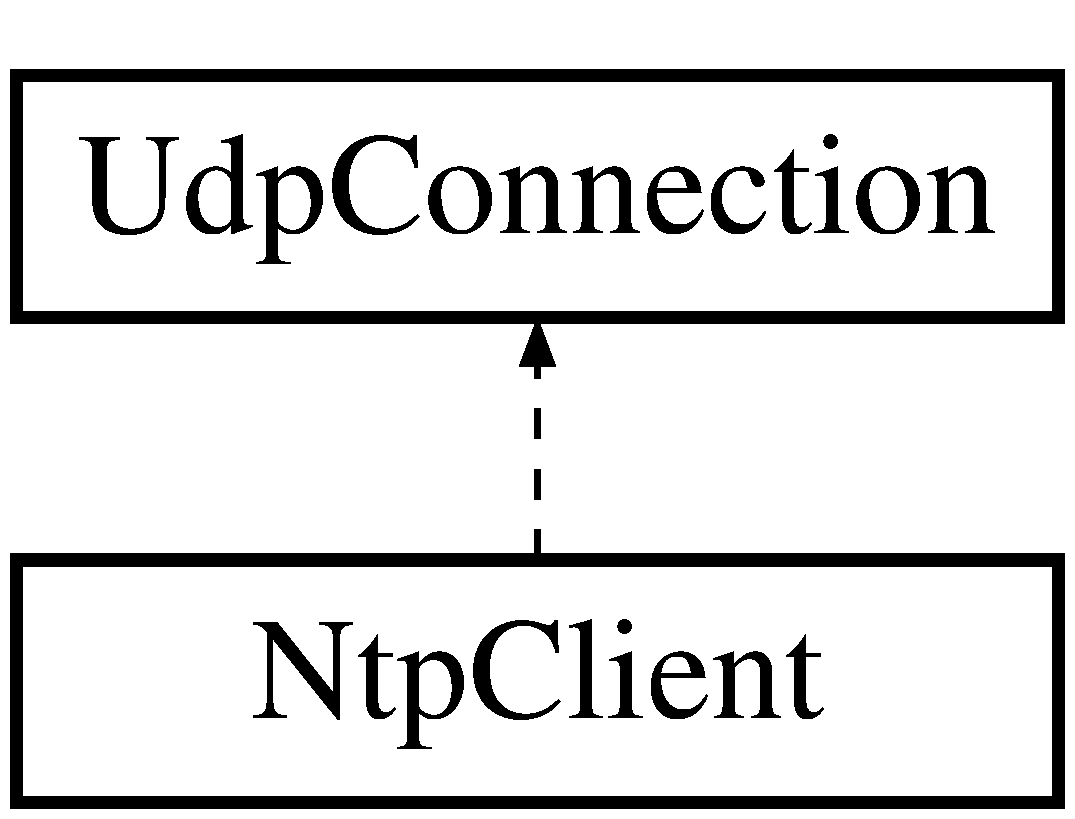
\includegraphics[height=2.000000cm]{class_ntp_client}
\end{center}
\end{figure}
\subsection*{Public Member Functions}
\begin{DoxyCompactItemize}
\item 
\hypertarget{class_ntp_client_a46add49d6f3467cddd98657adc52022d}{}{\bfseries Ntp\+Client} (Ntp\+Time\+Result\+Callback on\+Time\+Received\+Cb)\label{class_ntp_client_a46add49d6f3467cddd98657adc52022d}

\item 
\hypertarget{class_ntp_client_ac91b12ec68dea642949c09019b42ced4}{}{\bfseries Ntp\+Client} (String req\+Server, int req\+Interval\+Seconds, Ntp\+Time\+Result\+Callback on\+Time\+Received\+Cb)\label{class_ntp_client_ac91b12ec68dea642949c09019b42ced4}

\item 
\hypertarget{class_ntp_client_ae161dd8cad61353e0090dcbf0f152420}{}{\bfseries Ntp\+Client} (String req\+Server, int req\+Interval\+Seconds, \hyperlink{class_delegate}{Ntp\+Client\+Result\+Callback} delegate\+Function=N\+U\+L\+L)\label{class_ntp_client_ae161dd8cad61353e0090dcbf0f152420}

\item 
\hypertarget{class_ntp_client_af02ed50c487b0572e4b00c6159a65b95}{}void {\bfseries request\+Time} ()\label{class_ntp_client_af02ed50c487b0572e4b00c6159a65b95}

\item 
\hypertarget{class_ntp_client_a85a38d86185c7967b4dfb8deed66f3fc}{}void {\bfseries set\+Ntp\+Server} (String server)\label{class_ntp_client_a85a38d86185c7967b4dfb8deed66f3fc}

\item 
\hypertarget{class_ntp_client_a2582e24cb2749e70c220d215da627393}{}void {\bfseries set\+Ntp\+Server} (\hyperlink{class_i_p_address}{I\+P\+Address} adress)\label{class_ntp_client_a2582e24cb2749e70c220d215da627393}

\item 
\hypertarget{class_ntp_client_a5f43fe41391992dd859301c9cf8505b2}{}void {\bfseries set\+Auto\+Query} (bool auto\+Query)\label{class_ntp_client_a5f43fe41391992dd859301c9cf8505b2}

\item 
\hypertarget{class_ntp_client_a801a30e8e1fc876699a8a71ec6cfcc70}{}void {\bfseries set\+Auto\+Query\+Interval} (int seconds)\label{class_ntp_client_a801a30e8e1fc876699a8a71ec6cfcc70}

\item 
\hypertarget{class_ntp_client_ab347aea16a3aba444e7636cfbfefbf0e}{}void {\bfseries set\+Auto\+Update\+System\+Clock} (bool auto\+Update\+Clock)\label{class_ntp_client_ab347aea16a3aba444e7636cfbfefbf0e}

\end{DoxyCompactItemize}
\subsection*{Protected Member Functions}
\begin{DoxyCompactItemize}
\item 
\hypertarget{class_ntp_client_af542fa6108dfc497145cee6228776115}{}int {\bfseries resolve\+Server} ()\label{class_ntp_client_af542fa6108dfc497145cee6228776115}

\item 
\hypertarget{class_ntp_client_acc2092a5f662df125d7dd6600dad5ec3}{}void {\bfseries on\+Receive} (\hyperlink{structpbuf}{pbuf} $\ast$buf, \hyperlink{class_i_p_address}{I\+P\+Address} remote\+I\+P, uint16\+\_\+t remote\+Port)\label{class_ntp_client_acc2092a5f662df125d7dd6600dad5ec3}

\end{DoxyCompactItemize}
\subsection*{Static Protected Member Functions}
\begin{DoxyCompactItemize}
\item 
\hypertarget{class_ntp_client_ab4015733d3546a6c1c5b787aab2afc85}{}static void {\bfseries static\+Dns\+Response} (const char $\ast$name, struct \hyperlink{structip__addr}{ip\+\_\+addr} $\ast$ip, void $\ast$arg)\label{class_ntp_client_ab4015733d3546a6c1c5b787aab2afc85}

\end{DoxyCompactItemize}
\subsection*{Protected Attributes}
\begin{DoxyCompactItemize}
\item 
\hypertarget{class_ntp_client_a3b8cfcd355c2100d3108e009e5a91d65}{}String {\bfseries server} = N\+T\+P\+\_\+\+S\+E\+R\+V\+E\+R\+\_\+\+D\+E\+F\+A\+U\+L\+T\label{class_ntp_client_a3b8cfcd355c2100d3108e009e5a91d65}

\item 
\hypertarget{class_ntp_client_a6d87e3e0b5c26d80a7bfe05e53c97f04}{}\hyperlink{class_i_p_address}{I\+P\+Address} {\bfseries server\+Address} = (uint32\+\_\+t)0\label{class_ntp_client_a6d87e3e0b5c26d80a7bfe05e53c97f04}

\item 
\hypertarget{class_ntp_client_aa59e45eab7e751bb8ee6d2a8585d4875}{}Ntp\+Time\+Result\+Callback {\bfseries on\+Completed} = nullptr\label{class_ntp_client_aa59e45eab7e751bb8ee6d2a8585d4875}

\item 
\hypertarget{class_ntp_client_a8c248c8594feb698893b0df65bb98ad9}{}\hyperlink{class_delegate}{Ntp\+Client\+Result\+Callback} {\bfseries delegate\+Completed} = nullptr\label{class_ntp_client_a8c248c8594feb698893b0df65bb98ad9}

\item 
\hypertarget{class_ntp_client_a3788a373550ccc201532d658c6326cd1}{}bool {\bfseries auto\+Update\+System\+Clock} = false\label{class_ntp_client_a3788a373550ccc201532d658c6326cd1}

\item 
\hypertarget{class_ntp_client_a4b68b70348203e1d13705de352bc5394}{}\hyperlink{class_timer}{Timer} {\bfseries auto\+Update\+Timer}\label{class_ntp_client_a4b68b70348203e1d13705de352bc5394}

\item 
\hypertarget{class_ntp_client_af98a2f994584ce9c20f951560c4825f3}{}\hyperlink{class_timer}{Timer} {\bfseries connection\+Timer}\label{class_ntp_client_af98a2f994584ce9c20f951560c4825f3}

\end{DoxyCompactItemize}


The documentation for this class was generated from the following files\+:\begin{DoxyCompactItemize}
\item 
Sming\+Core/\+Network/Ntp\+Client.\+h\item 
Sming\+Core/\+Network/Ntp\+Client.\+cpp\end{DoxyCompactItemize}

\hypertarget{class_one_wire}{}\section{One\+Wire Class Reference}
\label{class_one_wire}\index{One\+Wire@{One\+Wire}}
\subsection*{Public Member Functions}
\begin{DoxyCompactItemize}
\item 
\hypertarget{class_one_wire_aa3f23dc51d861a8d257648c507b14e8d}{}{\bfseries One\+Wire} (uint8\+\_\+t pin)\label{class_one_wire_aa3f23dc51d861a8d257648c507b14e8d}

\item 
\hypertarget{class_one_wire_acc6da81f961028fe654497c1e45f19a3}{}void {\bfseries begin} ()\label{class_one_wire_acc6da81f961028fe654497c1e45f19a3}

\item 
\hypertarget{class_one_wire_a6a742a9112392567eae3d06dde067c07}{}uint8\+\_\+t {\bfseries reset} (void)\label{class_one_wire_a6a742a9112392567eae3d06dde067c07}

\item 
\hypertarget{class_one_wire_accf808390abd63d3c7bce35677784384}{}void {\bfseries select} (const uint8\+\_\+t rom\mbox{[}8\mbox{]})\label{class_one_wire_accf808390abd63d3c7bce35677784384}

\item 
\hypertarget{class_one_wire_ae3780e2b0ea2ebf6be88298412ac7798}{}void {\bfseries skip} (void)\label{class_one_wire_ae3780e2b0ea2ebf6be88298412ac7798}

\item 
\hypertarget{class_one_wire_a843e9e7e57ed615b4880be0b76b40b7d}{}void {\bfseries write} (uint8\+\_\+t v, uint8\+\_\+t power=0)\label{class_one_wire_a843e9e7e57ed615b4880be0b76b40b7d}

\item 
\hypertarget{class_one_wire_a0fc1e0bdc2ab1f062c98567fa60a69ae}{}void {\bfseries write\+\_\+bytes} (const uint8\+\_\+t $\ast$buf, uint16\+\_\+t count, bool power=0)\label{class_one_wire_a0fc1e0bdc2ab1f062c98567fa60a69ae}

\item 
\hypertarget{class_one_wire_afd9bdb8b5a5b69b394dfc76352e00e21}{}uint8\+\_\+t {\bfseries read} (void)\label{class_one_wire_afd9bdb8b5a5b69b394dfc76352e00e21}

\item 
\hypertarget{class_one_wire_a2407440e8e25b624617593f8ad6447d4}{}void {\bfseries read\+\_\+bytes} (uint8\+\_\+t $\ast$buf, uint16\+\_\+t count)\label{class_one_wire_a2407440e8e25b624617593f8ad6447d4}

\item 
\hypertarget{class_one_wire_a6bbc58276d1cb08653dab3ea35378f94}{}void {\bfseries write\+\_\+bit} (uint8\+\_\+t v)\label{class_one_wire_a6bbc58276d1cb08653dab3ea35378f94}

\item 
\hypertarget{class_one_wire_aeae4c2798b70d9d0ba3091c03ee2d056}{}uint8\+\_\+t {\bfseries read\+\_\+bit} (void)\label{class_one_wire_aeae4c2798b70d9d0ba3091c03ee2d056}

\item 
\hypertarget{class_one_wire_aa8e0f62e830ad05d8035e55c7a309256}{}void {\bfseries depower} (void)\label{class_one_wire_aa8e0f62e830ad05d8035e55c7a309256}

\item 
\hypertarget{class_one_wire_aae5efdf67928b5ee312ab7d7906416fa}{}void {\bfseries reset\+\_\+search} ()\label{class_one_wire_aae5efdf67928b5ee312ab7d7906416fa}

\item 
\hypertarget{class_one_wire_a0a1b8457adb609a693b865dd474e5116}{}void {\bfseries target\+\_\+search} (uint8\+\_\+t family\+\_\+code)\label{class_one_wire_a0a1b8457adb609a693b865dd474e5116}

\item 
\hypertarget{class_one_wire_a383dc74fc9f8a27b76366a2859c3820a}{}uint8\+\_\+t {\bfseries search} (uint8\+\_\+t $\ast$new\+Addr)\label{class_one_wire_a383dc74fc9f8a27b76366a2859c3820a}

\end{DoxyCompactItemize}
\subsection*{Static Public Member Functions}
\begin{DoxyCompactItemize}
\item 
\hypertarget{class_one_wire_ae3486a669581b750e4fdf3f3a12b05f1}{}static uint8\+\_\+t {\bfseries crc8} (const uint8\+\_\+t $\ast$addr, uint8\+\_\+t len)\label{class_one_wire_ae3486a669581b750e4fdf3f3a12b05f1}

\item 
\hypertarget{class_one_wire_a089c502d26caca5214264261db82d011}{}static bool {\bfseries check\+\_\+crc16} (const uint8\+\_\+t $\ast$input, uint16\+\_\+t len, const uint8\+\_\+t $\ast$inverted\+\_\+crc, uint16\+\_\+t crc=0)\label{class_one_wire_a089c502d26caca5214264261db82d011}

\item 
\hypertarget{class_one_wire_a685131803ff9bd250926de68fb477998}{}static uint16\+\_\+t {\bfseries crc16} (const uint8\+\_\+t $\ast$input, uint16\+\_\+t len, uint16\+\_\+t crc=0)\label{class_one_wire_a685131803ff9bd250926de68fb477998}

\end{DoxyCompactItemize}


The documentation for this class was generated from the following files\+:\begin{DoxyCompactItemize}
\item 
Libraries/\+One\+Wire/One\+Wire.\+h\item 
Libraries/\+One\+Wire/One\+Wire.\+cpp\end{DoxyCompactItemize}

\hypertarget{structpbuf}{}\section{pbuf Struct Reference}
\label{structpbuf}\index{pbuf@{pbuf}}
\subsection*{Public Attributes}
\begin{DoxyCompactItemize}
\item 
struct \hyperlink{structpbuf}{pbuf} $\ast$ \hyperlink{structpbuf_a5e5763c94fd18d78937b0b58ce7df341}{next}
\item 
void $\ast$ \hyperlink{structpbuf_a8d32dc3e964369d4eec638fc37fbc460}{payload}
\item 
u16\+\_\+t \hyperlink{structpbuf_a5259e7ec29bab9c0999b64f2e86b411f}{tot\+\_\+len}
\item 
u16\+\_\+t \hyperlink{structpbuf_a6f82449625e36e294f5d210268c0703f}{len}
\item 
u8\+\_\+t \hyperlink{structpbuf_afd7bff5210a022424caa97d2f25fe8e6}{type}
\item 
u8\+\_\+t \hyperlink{structpbuf_aa4d1af2cab3d9280d29212095b5b872a}{flags}
\item 
u16\+\_\+t \hyperlink{structpbuf_a18e2c02942feb1baa3756fcd585b6731}{ref}
\item 
\hypertarget{structpbuf_a49924e7a48749a7ed303f64cf3c8d235}{}void $\ast$ {\bfseries eb}\label{structpbuf_a49924e7a48749a7ed303f64cf3c8d235}

\end{DoxyCompactItemize}


\subsection{Member Data Documentation}
\hypertarget{structpbuf_aa4d1af2cab3d9280d29212095b5b872a}{}\index{pbuf@{pbuf}!flags@{flags}}
\index{flags@{flags}!pbuf@{pbuf}}
\subsubsection[{flags}]{\setlength{\rightskip}{0pt plus 5cm}u8\+\_\+t pbuf\+::flags}\label{structpbuf_aa4d1af2cab3d9280d29212095b5b872a}
misc flags \hypertarget{structpbuf_a6f82449625e36e294f5d210268c0703f}{}\index{pbuf@{pbuf}!len@{len}}
\index{len@{len}!pbuf@{pbuf}}
\subsubsection[{len}]{\setlength{\rightskip}{0pt plus 5cm}u16\+\_\+t pbuf\+::len}\label{structpbuf_a6f82449625e36e294f5d210268c0703f}
length of this buffer \hypertarget{structpbuf_a5e5763c94fd18d78937b0b58ce7df341}{}\index{pbuf@{pbuf}!next@{next}}
\index{next@{next}!pbuf@{pbuf}}
\subsubsection[{next}]{\setlength{\rightskip}{0pt plus 5cm}struct {\bf pbuf}$\ast$ pbuf\+::next}\label{structpbuf_a5e5763c94fd18d78937b0b58ce7df341}
next pbuf in singly linked pbuf chain \hypertarget{structpbuf_a8d32dc3e964369d4eec638fc37fbc460}{}\index{pbuf@{pbuf}!payload@{payload}}
\index{payload@{payload}!pbuf@{pbuf}}
\subsubsection[{payload}]{\setlength{\rightskip}{0pt plus 5cm}void$\ast$ pbuf\+::payload}\label{structpbuf_a8d32dc3e964369d4eec638fc37fbc460}
pointer to the actual data in the buffer \hypertarget{structpbuf_a18e2c02942feb1baa3756fcd585b6731}{}\index{pbuf@{pbuf}!ref@{ref}}
\index{ref@{ref}!pbuf@{pbuf}}
\subsubsection[{ref}]{\setlength{\rightskip}{0pt plus 5cm}u16\+\_\+t pbuf\+::ref}\label{structpbuf_a18e2c02942feb1baa3756fcd585b6731}
the reference count always equals the number of pointers that refer to this pbuf. This can be pointers from an application, the stack itself, or pbuf-\/$>$next pointers from a chain. \hypertarget{structpbuf_a5259e7ec29bab9c0999b64f2e86b411f}{}\index{pbuf@{pbuf}!tot\+\_\+len@{tot\+\_\+len}}
\index{tot\+\_\+len@{tot\+\_\+len}!pbuf@{pbuf}}
\subsubsection[{tot\+\_\+len}]{\setlength{\rightskip}{0pt plus 5cm}u16\+\_\+t pbuf\+::tot\+\_\+len}\label{structpbuf_a5259e7ec29bab9c0999b64f2e86b411f}
total length of this buffer and all next buffers in chain belonging to the same packet.

For non-\/queue packet chains this is the invariant\+: p-\/$>$tot\+\_\+len == p-\/$>$len + (p-\/$>$next? p-\/$>$next-\/$>$tot\+\_\+len\+: 0) \hypertarget{structpbuf_afd7bff5210a022424caa97d2f25fe8e6}{}\index{pbuf@{pbuf}!type@{type}}
\index{type@{type}!pbuf@{pbuf}}
\subsubsection[{type}]{\setlength{\rightskip}{0pt plus 5cm}u8\+\_\+t pbuf\+::type}\label{structpbuf_afd7bff5210a022424caa97d2f25fe8e6}
pbuf\+\_\+type as u8\+\_\+t instead of enum to save space 

The documentation for this struct was generated from the following file\+:\begin{DoxyCompactItemize}
\item 
system/include/lwip/pbuf.\+h\end{DoxyCompactItemize}

\hypertarget{structping__msg}{}\section{ping\+\_\+msg Struct Reference}
\label{structping__msg}\index{ping\+\_\+msg@{ping\+\_\+msg}}
\subsection*{Public Attributes}
\begin{DoxyCompactItemize}
\item 
\hypertarget{structping__msg_a154e32c7ee9f5c7897cfebd588601fa4}{}struct \hyperlink{structping__option}{ping\+\_\+option} $\ast$ {\bfseries ping\+\_\+opt}\label{structping__msg_a154e32c7ee9f5c7897cfebd588601fa4}

\item 
\hypertarget{structping__msg_a948f797503887ac1ed436f51385e4c00}{}struct raw\+\_\+pcb $\ast$ {\bfseries ping\+\_\+pcb}\label{structping__msg_a948f797503887ac1ed436f51385e4c00}

\item 
\hypertarget{structping__msg_a2c6d986481e35257721a8e5704e8b3d3}{}uint32 {\bfseries ping\+\_\+start}\label{structping__msg_a2c6d986481e35257721a8e5704e8b3d3}

\item 
\hypertarget{structping__msg_a4c4e086c4da3df826b116d58bf27ed0a}{}uint32 {\bfseries ping\+\_\+sent}\label{structping__msg_a4c4e086c4da3df826b116d58bf27ed0a}

\item 
\hypertarget{structping__msg_afdb5a471ef49fe050786c61724741ecc}{}uint32 {\bfseries timeout\+\_\+count}\label{structping__msg_afdb5a471ef49fe050786c61724741ecc}

\item 
\hypertarget{structping__msg_aad192e8bebb590a098d811cef32b0dda}{}uint32 {\bfseries max\+\_\+count}\label{structping__msg_aad192e8bebb590a098d811cef32b0dda}

\item 
\hypertarget{structping__msg_ae7a55a611561cc873d4f200256c5efd2}{}uint32 {\bfseries sent\+\_\+count}\label{structping__msg_ae7a55a611561cc873d4f200256c5efd2}

\item 
\hypertarget{structping__msg_a52a28f6f1dfc241d7050e93195ee6035}{}uint32 {\bfseries coarse\+\_\+time}\label{structping__msg_a52a28f6f1dfc241d7050e93195ee6035}

\end{DoxyCompactItemize}


The documentation for this struct was generated from the following file\+:\begin{DoxyCompactItemize}
\item 
system/include/lwip/app/ping.\+h\end{DoxyCompactItemize}

\hypertarget{structping__option}{}\section{ping\+\_\+option Struct Reference}
\label{structping__option}\index{ping\+\_\+option@{ping\+\_\+option}}
\subsection*{Public Attributes}
\begin{DoxyCompactItemize}
\item 
\hypertarget{structping__option_aaeae4d79766b00e0c0775a879822900b}{}uint32 {\bfseries count}\label{structping__option_aaeae4d79766b00e0c0775a879822900b}

\item 
\hypertarget{structping__option_a5651a366b7aaae8cbb77dd2f339aafc1}{}uint32 {\bfseries ip}\label{structping__option_a5651a366b7aaae8cbb77dd2f339aafc1}

\item 
\hypertarget{structping__option_ac067c82d950fc709d9dbf3f30a2a4eb0}{}uint32 {\bfseries coarse\+\_\+time}\label{structping__option_ac067c82d950fc709d9dbf3f30a2a4eb0}

\item 
\hypertarget{structping__option_adaff73ea4b12a2b27fccf3e0bb4d5d22}{}ping\+\_\+recv\+\_\+function {\bfseries recv\+\_\+function}\label{structping__option_adaff73ea4b12a2b27fccf3e0bb4d5d22}

\item 
\hypertarget{structping__option_ab7be798b88b78aa0a2d299dd8c8d0f7f}{}ping\+\_\+sent\+\_\+function {\bfseries sent\+\_\+function}\label{structping__option_ab7be798b88b78aa0a2d299dd8c8d0f7f}

\item 
\hypertarget{structping__option_a1f15b064c15989adbdfec979d41409e2}{}void $\ast$ {\bfseries reverse}\label{structping__option_a1f15b064c15989adbdfec979d41409e2}

\end{DoxyCompactItemize}


The documentation for this struct was generated from the following file\+:\begin{DoxyCompactItemize}
\item 
system/include/lwip/app/ping.\+h\end{DoxyCompactItemize}

\hypertarget{structping__resp}{}\section{ping\+\_\+resp Struct Reference}
\label{structping__resp}\index{ping\+\_\+resp@{ping\+\_\+resp}}
\subsection*{Public Attributes}
\begin{DoxyCompactItemize}
\item 
\hypertarget{structping__resp_a6fa551dcaa02b1972bcb033a77d9c3fb}{}uint32 {\bfseries total\+\_\+count}\label{structping__resp_a6fa551dcaa02b1972bcb033a77d9c3fb}

\item 
\hypertarget{structping__resp_aa3d8544071979aa91c63dfc0965266ee}{}uint32 {\bfseries resp\+\_\+time}\label{structping__resp_aa3d8544071979aa91c63dfc0965266ee}

\item 
\hypertarget{structping__resp_a7f98b4759b001fff0de971272a67520b}{}uint32 {\bfseries seqno}\label{structping__resp_a7f98b4759b001fff0de971272a67520b}

\item 
\hypertarget{structping__resp_a8374619f387f89cfd63dc103a7bc13f9}{}uint32 {\bfseries timeout\+\_\+count}\label{structping__resp_a8374619f387f89cfd63dc103a7bc13f9}

\item 
\hypertarget{structping__resp_a04b0cdcd564844cc5625e59e13b37102}{}uint32 {\bfseries bytes}\label{structping__resp_a04b0cdcd564844cc5625e59e13b37102}

\item 
\hypertarget{structping__resp_a58cb7aa28712969e0163f32a934e3a02}{}uint32 {\bfseries total\+\_\+bytes}\label{structping__resp_a58cb7aa28712969e0163f32a934e3a02}

\item 
\hypertarget{structping__resp_a7d5bf320e3d8b1621532b520ee4e2bc1}{}uint32 {\bfseries total\+\_\+time}\label{structping__resp_a7d5bf320e3d8b1621532b520ee4e2bc1}

\item 
\hypertarget{structping__resp_acd57b9c77bf5aab9f049df33a66e0e65}{}sint8 {\bfseries ping\+\_\+err}\label{structping__resp_acd57b9c77bf5aab9f049df33a66e0e65}

\end{DoxyCompactItemize}


The documentation for this struct was generated from the following file\+:\begin{DoxyCompactItemize}
\item 
system/include/lwip/app/ping.\+h\end{DoxyCompactItemize}

\hypertarget{class_arduino_json_1_1_internals_1_1_prettyfier}{}\section{Arduino\+Json\+:\+:Internals\+:\+:Prettyfier Class Reference}
\label{class_arduino_json_1_1_internals_1_1_prettyfier}\index{Arduino\+Json\+::\+Internals\+::\+Prettyfier@{Arduino\+Json\+::\+Internals\+::\+Prettyfier}}
Inheritance diagram for Arduino\+Json\+:\+:Internals\+:\+:Prettyfier\+:\begin{figure}[H]
\begin{center}
\leavevmode
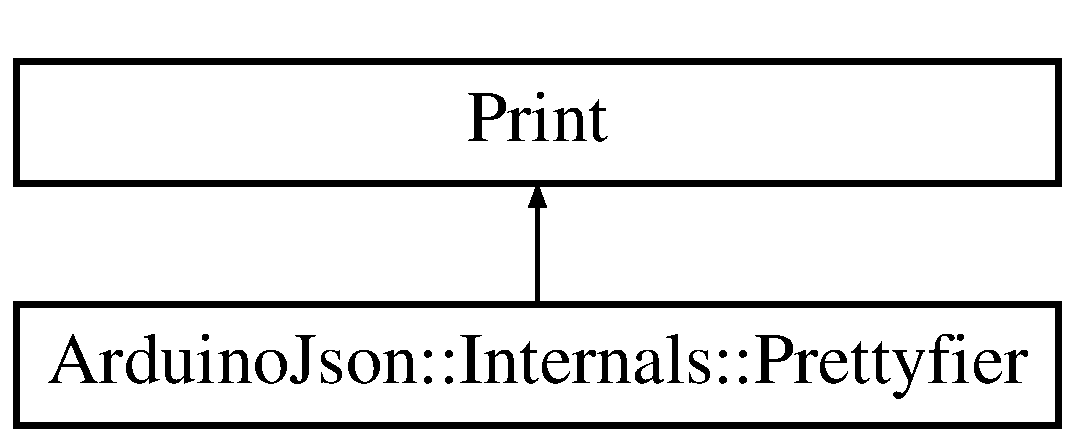
\includegraphics[height=2.000000cm]{class_arduino_json_1_1_internals_1_1_prettyfier}
\end{center}
\end{figure}
\subsection*{Public Member Functions}
\begin{DoxyCompactItemize}
\item 
\hypertarget{class_arduino_json_1_1_internals_1_1_prettyfier_acefa5f4571cc75c854ae41032be2a0db}{}{\bfseries Prettyfier} (\hyperlink{class_arduino_json_1_1_internals_1_1_indented_print}{Indented\+Print} \&p)\label{class_arduino_json_1_1_internals_1_1_prettyfier_acefa5f4571cc75c854ae41032be2a0db}

\item 
\hypertarget{class_arduino_json_1_1_internals_1_1_prettyfier_af532eac1f8b66a6b9270a873d4af0e56}{}virtual size\+\_\+t {\bfseries write} (uint8\+\_\+t)\label{class_arduino_json_1_1_internals_1_1_prettyfier_af532eac1f8b66a6b9270a873d4af0e56}

\end{DoxyCompactItemize}


The documentation for this class was generated from the following files\+:\begin{DoxyCompactItemize}
\item 
Services/\+Arduino\+Json/include/\+Arduino\+Json/\+Internals/Prettyfier.\+hpp\item 
Services/\+Arduino\+Json/src/\+Internals/Prettyfier.\+cpp\end{DoxyCompactItemize}

\hypertarget{class_printable}{}\section{Printable Class Reference}
\label{class_printable}\index{Printable@{Printable}}
Inheritance diagram for Printable\+:\begin{figure}[H]
\begin{center}
\leavevmode
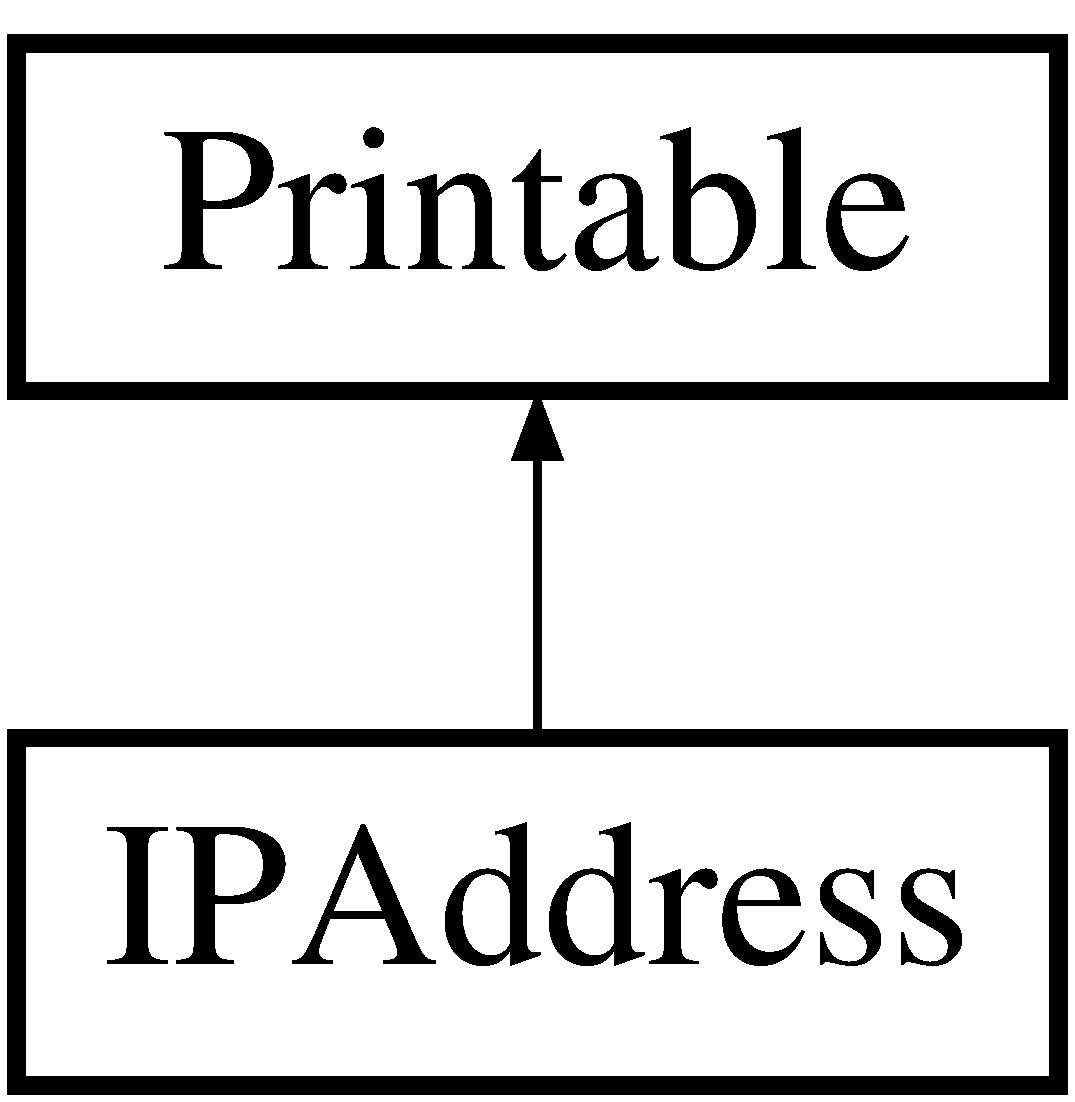
\includegraphics[height=2.000000cm]{class_printable}
\end{center}
\end{figure}
\subsection*{Public Member Functions}
\begin{DoxyCompactItemize}
\item 
\hypertarget{class_printable_a2c5776bc55c0a3a5675bba9d4d8e3681}{}virtual size\+\_\+t {\bfseries print\+To} (Print \&p) const =0\label{class_printable_a2c5776bc55c0a3a5675bba9d4d8e3681}

\end{DoxyCompactItemize}


The documentation for this class was generated from the following file\+:\begin{DoxyCompactItemize}
\item 
Wiring/Printable.\+h\end{DoxyCompactItemize}

\hypertarget{class_arduino_json_1_1_internals_1_1_quoted_string}{}\section{Arduino\+Json\+:\+:Internals\+:\+:Quoted\+String Class Reference}
\label{class_arduino_json_1_1_internals_1_1_quoted_string}\index{Arduino\+Json\+::\+Internals\+::\+Quoted\+String@{Arduino\+Json\+::\+Internals\+::\+Quoted\+String}}
\subsection*{Static Public Member Functions}
\begin{DoxyCompactItemize}
\item 
\hypertarget{class_arduino_json_1_1_internals_1_1_quoted_string_a2719c00c59773ec60720e03c8a9b20c4}{}static size\+\_\+t {\bfseries print\+To} (const char $\ast$, Print \&)\label{class_arduino_json_1_1_internals_1_1_quoted_string_a2719c00c59773ec60720e03c8a9b20c4}

\item 
\hypertarget{class_arduino_json_1_1_internals_1_1_quoted_string_acb881b13714b9ae36a67ba8e33181bf1}{}static char $\ast$ {\bfseries extract\+From} (char $\ast$input, char $\ast$$\ast$end)\label{class_arduino_json_1_1_internals_1_1_quoted_string_acb881b13714b9ae36a67ba8e33181bf1}

\end{DoxyCompactItemize}


The documentation for this class was generated from the following files\+:\begin{DoxyCompactItemize}
\item 
Services/\+Arduino\+Json/include/\+Arduino\+Json/\+Internals/Quoted\+String.\+hpp\item 
Services/\+Arduino\+Json/src/\+Internals/Quoted\+String.\+cpp\end{DoxyCompactItemize}

\hypertarget{struct_rcv_msg_buff}{}\section{Rcv\+Msg\+Buff Struct Reference}
\label{struct_rcv_msg_buff}\index{Rcv\+Msg\+Buff@{Rcv\+Msg\+Buff}}
\subsection*{Public Attributes}
\begin{DoxyCompactItemize}
\item 
\hypertarget{struct_rcv_msg_buff_a100e2cdf15349ae18fca2fbb67d5845b}{}uint32 {\bfseries Rcv\+Buff\+Size}\label{struct_rcv_msg_buff_a100e2cdf15349ae18fca2fbb67d5845b}

\item 
\hypertarget{struct_rcv_msg_buff_a62921396b7988d167cdbfadaeaafa1ad}{}uint8 $\ast$ {\bfseries p\+Rcv\+Msg\+Buff}\label{struct_rcv_msg_buff_a62921396b7988d167cdbfadaeaafa1ad}

\item 
\hypertarget{struct_rcv_msg_buff_adcdca9d20078d517946d66d355579693}{}uint8 $\ast$ {\bfseries p\+Write\+Pos}\label{struct_rcv_msg_buff_adcdca9d20078d517946d66d355579693}

\item 
\hypertarget{struct_rcv_msg_buff_aee50309a2497fffef33577ab901fe2cc}{}uint8 $\ast$ {\bfseries p\+Read\+Pos}\label{struct_rcv_msg_buff_aee50309a2497fffef33577ab901fe2cc}

\item 
\hypertarget{struct_rcv_msg_buff_a142735d44b7fefc09c930d58b5e70d4d}{}uint8 {\bfseries Trig\+Lvl}\label{struct_rcv_msg_buff_a142735d44b7fefc09c930d58b5e70d4d}

\item 
\hypertarget{struct_rcv_msg_buff_a834e373c1fa1798f35fa38fd197674e0}{}Rcv\+Msg\+Buff\+State {\bfseries Buff\+State}\label{struct_rcv_msg_buff_a834e373c1fa1798f35fa38fd197674e0}

\end{DoxyCompactItemize}


The documentation for this struct was generated from the following file\+:\begin{DoxyCompactItemize}
\item 
system/include/espinc/uart.\+h\end{DoxyCompactItemize}

\hypertarget{class_arduino_json_1_1_internals_1_1_reference_type}{}\section{Arduino\+Json\+:\+:Internals\+:\+:Reference\+Type Class Reference}
\label{class_arduino_json_1_1_internals_1_1_reference_type}\index{Arduino\+Json\+::\+Internals\+::\+Reference\+Type@{Arduino\+Json\+::\+Internals\+::\+Reference\+Type}}
Inheritance diagram for Arduino\+Json\+:\+:Internals\+:\+:Reference\+Type\+:\begin{figure}[H]
\begin{center}
\leavevmode
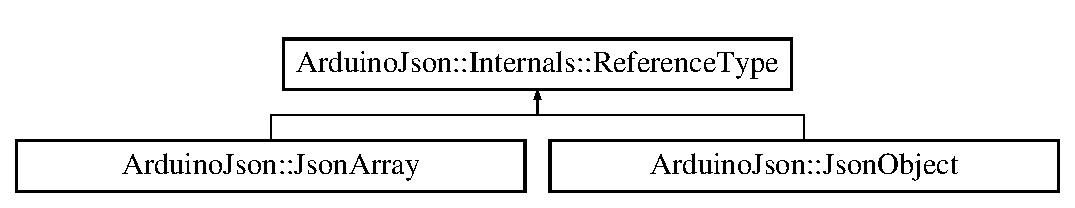
\includegraphics[height=2.000000cm]{class_arduino_json_1_1_internals_1_1_reference_type}
\end{center}
\end{figure}
\subsection*{Public Member Functions}
\begin{DoxyCompactItemize}
\item 
\hypertarget{class_arduino_json_1_1_internals_1_1_reference_type_a810d0e47f100480caba6b3f23e9a5c1c}{}bool {\bfseries operator==} (const \hyperlink{class_arduino_json_1_1_internals_1_1_reference_type}{Reference\+Type} \&other) const \label{class_arduino_json_1_1_internals_1_1_reference_type_a810d0e47f100480caba6b3f23e9a5c1c}

\item 
\hypertarget{class_arduino_json_1_1_internals_1_1_reference_type_ae68ffa6faef1a7bbc79469aa3c46278a}{}bool {\bfseries operator!=} (const \hyperlink{class_arduino_json_1_1_internals_1_1_reference_type}{Reference\+Type} \&other) const \label{class_arduino_json_1_1_internals_1_1_reference_type_ae68ffa6faef1a7bbc79469aa3c46278a}

\end{DoxyCompactItemize}


The documentation for this class was generated from the following file\+:\begin{DoxyCompactItemize}
\item 
Services/\+Arduino\+Json/include/\+Arduino\+Json/\+Internals/Reference\+Type.\+hpp\end{DoxyCompactItemize}

\hypertarget{class_soft_i2c_master}{}\section{Soft\+I2c\+Master Class Reference}
\label{class_soft_i2c_master}\index{Soft\+I2c\+Master@{Soft\+I2c\+Master}}


Software I2\+C master class.  




{\ttfamily \#include $<$I2c\+Master.\+h$>$}

Inheritance diagram for Soft\+I2c\+Master\+:\begin{figure}[H]
\begin{center}
\leavevmode
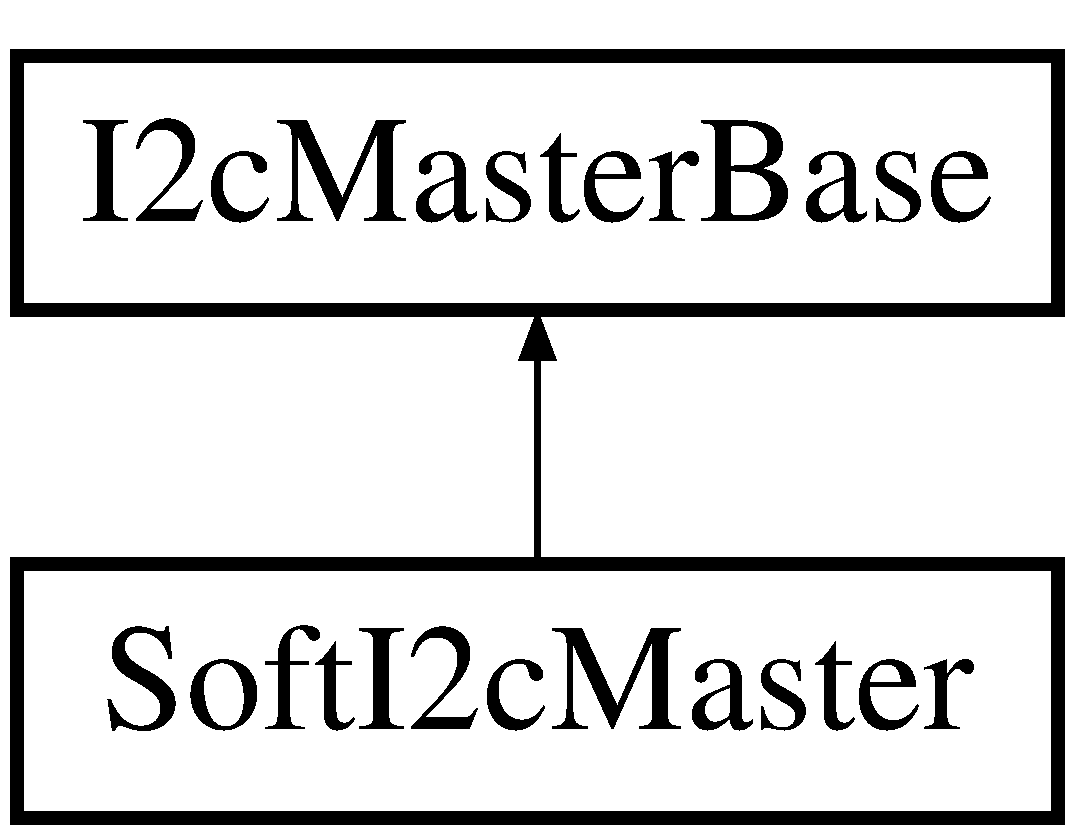
\includegraphics[height=2.000000cm]{class_soft_i2c_master}
\end{center}
\end{figure}
\subsection*{Public Member Functions}
\begin{DoxyCompactItemize}
\item 
\hyperlink{class_soft_i2c_master_a1e583d6f81bc43e403d315f05702919a}{Soft\+I2c\+Master} (uint8\+\_\+t sda\+Pin, uint8\+\_\+t scl\+Pin)
\item 
uint8\+\_\+t \hyperlink{class_soft_i2c_master_a56993378a66a702113eef640d8c82ea9}{read} (uint8\+\_\+t last)
\item 
bool \hyperlink{class_soft_i2c_master_a4ec0db661a654943888df023b233bcc5}{restart} (uint8\+\_\+t address\+R\+W)
\item 
bool \hyperlink{class_soft_i2c_master_a66a6298702caed4f52537ef372307699}{start} (uint8\+\_\+t address\+R\+W)
\item 
void \hyperlink{class_soft_i2c_master_ad8f52e1cbf15894472881afe439afa02}{stop} (void)
\item 
bool \hyperlink{class_soft_i2c_master_abcce5d83ae63dc61c2662be4a934d083}{write} (uint8\+\_\+t b)
\end{DoxyCompactItemize}


\subsection{Detailed Description}
Software I2\+C master class. 

\subsection{Constructor \& Destructor Documentation}
\hypertarget{class_soft_i2c_master_a1e583d6f81bc43e403d315f05702919a}{}\index{Soft\+I2c\+Master@{Soft\+I2c\+Master}!Soft\+I2c\+Master@{Soft\+I2c\+Master}}
\index{Soft\+I2c\+Master@{Soft\+I2c\+Master}!Soft\+I2c\+Master@{Soft\+I2c\+Master}}
\subsubsection[{Soft\+I2c\+Master}]{\setlength{\rightskip}{0pt plus 5cm}Soft\+I2c\+Master\+::\+Soft\+I2c\+Master (
\begin{DoxyParamCaption}
\item[{uint8\+\_\+t}]{sda\+Pin, }
\item[{uint8\+\_\+t}]{scl\+Pin}
\end{DoxyParamCaption}
)}\label{class_soft_i2c_master_a1e583d6f81bc43e403d315f05702919a}
Initialize S\+C\+L/\+S\+D\+A pins and set the bus high.


\begin{DoxyParams}[1]{Parameters}
\mbox{\tt in}  & {\em sda\+Pin} & The software S\+D\+A pin number.\\
\hline
\mbox{\tt in}  & {\em scl\+Pin} & The software S\+C\+L pin number. \\
\hline
\end{DoxyParams}


\subsection{Member Function Documentation}
\hypertarget{class_soft_i2c_master_a56993378a66a702113eef640d8c82ea9}{}\index{Soft\+I2c\+Master@{Soft\+I2c\+Master}!read@{read}}
\index{read@{read}!Soft\+I2c\+Master@{Soft\+I2c\+Master}}
\subsubsection[{read}]{\setlength{\rightskip}{0pt plus 5cm}uint8\+\_\+t Soft\+I2c\+Master\+::read (
\begin{DoxyParamCaption}
\item[{uint8\+\_\+t}]{last}
\end{DoxyParamCaption}
)\hspace{0.3cm}{\ttfamily [virtual]}}\label{class_soft_i2c_master_a56993378a66a702113eef640d8c82ea9}
Read a byte and send Ack if more reads follow else Nak to terminate read.


\begin{DoxyParams}[1]{Parameters}
\mbox{\tt in}  & {\em last} & Set true to terminate the read else false.\\
\hline
\end{DoxyParams}
\begin{DoxyReturn}{Returns}
The byte read from the I2\+C bus. 
\end{DoxyReturn}


Implements \hyperlink{class_i2c_master_base_ab0642665deb11295592d3e46c8baaefa}{I2c\+Master\+Base}.

\hypertarget{class_soft_i2c_master_a4ec0db661a654943888df023b233bcc5}{}\index{Soft\+I2c\+Master@{Soft\+I2c\+Master}!restart@{restart}}
\index{restart@{restart}!Soft\+I2c\+Master@{Soft\+I2c\+Master}}
\subsubsection[{restart}]{\setlength{\rightskip}{0pt plus 5cm}bool Soft\+I2c\+Master\+::restart (
\begin{DoxyParamCaption}
\item[{uint8\+\_\+t}]{address\+R\+W}
\end{DoxyParamCaption}
)\hspace{0.3cm}{\ttfamily [virtual]}}\label{class_soft_i2c_master_a4ec0db661a654943888df023b233bcc5}
Issue a restart condition.


\begin{DoxyParams}[1]{Parameters}
\mbox{\tt in}  & {\em address\+R\+W} & I2\+C address with read/write bit.\\
\hline
\end{DoxyParams}
\begin{DoxyReturn}{Returns}
The value true, 1, for success or false, 0, for failure. 
\end{DoxyReturn}


Implements \hyperlink{class_i2c_master_base_a3ccb7274e45f8842f5748d5ae9931dd0}{I2c\+Master\+Base}.

\hypertarget{class_soft_i2c_master_a66a6298702caed4f52537ef372307699}{}\index{Soft\+I2c\+Master@{Soft\+I2c\+Master}!start@{start}}
\index{start@{start}!Soft\+I2c\+Master@{Soft\+I2c\+Master}}
\subsubsection[{start}]{\setlength{\rightskip}{0pt plus 5cm}bool Soft\+I2c\+Master\+::start (
\begin{DoxyParamCaption}
\item[{uint8\+\_\+t}]{address\+R\+W}
\end{DoxyParamCaption}
)\hspace{0.3cm}{\ttfamily [virtual]}}\label{class_soft_i2c_master_a66a6298702caed4f52537ef372307699}
Issue a start condition.


\begin{DoxyParams}[1]{Parameters}
\mbox{\tt in}  & {\em address\+R\+W} & I2\+C address with read/write bit.\\
\hline
\end{DoxyParams}
\begin{DoxyReturn}{Returns}
The value true, 1, for success or false, 0, for failure. 
\end{DoxyReturn}


Implements \hyperlink{class_i2c_master_base_adf5e98b79dec8f7b5a43c2ec8f2f9f7a}{I2c\+Master\+Base}.

\hypertarget{class_soft_i2c_master_ad8f52e1cbf15894472881afe439afa02}{}\index{Soft\+I2c\+Master@{Soft\+I2c\+Master}!stop@{stop}}
\index{stop@{stop}!Soft\+I2c\+Master@{Soft\+I2c\+Master}}
\subsubsection[{stop}]{\setlength{\rightskip}{0pt plus 5cm}void Soft\+I2c\+Master\+::stop (
\begin{DoxyParamCaption}
\item[{void}]{}
\end{DoxyParamCaption}
)\hspace{0.3cm}{\ttfamily [virtual]}}\label{class_soft_i2c_master_ad8f52e1cbf15894472881afe439afa02}
Issue a stop condition. 

Implements \hyperlink{class_i2c_master_base_a0c4f54aea3b04ed699efc0fa684712c7}{I2c\+Master\+Base}.

\hypertarget{class_soft_i2c_master_abcce5d83ae63dc61c2662be4a934d083}{}\index{Soft\+I2c\+Master@{Soft\+I2c\+Master}!write@{write}}
\index{write@{write}!Soft\+I2c\+Master@{Soft\+I2c\+Master}}
\subsubsection[{write}]{\setlength{\rightskip}{0pt plus 5cm}bool Soft\+I2c\+Master\+::write (
\begin{DoxyParamCaption}
\item[{uint8\+\_\+t}]{data}
\end{DoxyParamCaption}
)\hspace{0.3cm}{\ttfamily [virtual]}}\label{class_soft_i2c_master_abcce5d83ae63dc61c2662be4a934d083}
Write a byte.


\begin{DoxyParams}[1]{Parameters}
\mbox{\tt in}  & {\em data} & The byte to send.\\
\hline
\end{DoxyParams}
\begin{DoxyReturn}{Returns}
The value true, 1, if the slave returned an Ack or false for Nak. 
\end{DoxyReturn}


Implements \hyperlink{class_i2c_master_base_aee4d48385a72b48a0a452ecfc2cd7fc0}{I2c\+Master\+Base}.



The documentation for this class was generated from the following files\+:\begin{DoxyCompactItemize}
\item 
Wiring/\hyperlink{_i2c_master_8h}{I2c\+Master.\+h}\item 
Wiring/I2c\+Master.\+cpp\end{DoxyCompactItemize}

\hypertarget{class_s_p_i_class}{}\section{S\+P\+I\+Class Class Reference}
\label{class_s_p_i_class}\index{S\+P\+I\+Class@{S\+P\+I\+Class}}
\subsection*{Public Member Functions}
\begin{DoxyCompactItemize}
\item 
\hypertarget{class_s_p_i_class_a424cda909940ec30730a22e90764cd59}{}{\bfseries S\+P\+I\+Class} (uint8\+\_\+t spi\+I\+D)\label{class_s_p_i_class_a424cda909940ec30730a22e90764cd59}

\item 
\hypertarget{class_s_p_i_class_a4a2646959a242f6af423b04734c003f0}{}void {\bfseries begin} ()\label{class_s_p_i_class_a4a2646959a242f6af423b04734c003f0}

\item 
\hypertarget{class_s_p_i_class_a79d89d8e3f5f1b003cb7b0aed2d77eab}{}void {\bfseries end} ()\label{class_s_p_i_class_a79d89d8e3f5f1b003cb7b0aed2d77eab}

\item 
\hypertarget{class_s_p_i_class_af453faad2fe2fd9c166e6690a19f476a}{}void {\bfseries transfer} (uint8\+\_\+t $\ast$data, uint8\+\_\+t count)\label{class_s_p_i_class_af453faad2fe2fd9c166e6690a19f476a}

\item 
\hypertarget{class_s_p_i_class_a3ffa792ef92b0d1c299c9ea1185552ee}{}byte {\bfseries transfer} (uint8\+\_\+t data)\label{class_s_p_i_class_a3ffa792ef92b0d1c299c9ea1185552ee}

\end{DoxyCompactItemize}
\subsection*{Protected Member Functions}
\begin{DoxyCompactItemize}
\item 
\hypertarget{class_s_p_i_class_a26a8fb6897c7da200412428be6bb9f9a}{}void {\bfseries write\+Data} (uint8\+\_\+t $\ast$data, uint8\+\_\+t number\+Byte)\label{class_s_p_i_class_a26a8fb6897c7da200412428be6bb9f9a}

\item 
\hypertarget{class_s_p_i_class_a6a4d99e2e3b867025e71f030ff756be2}{}void {\bfseries read\+Data} (uint8\+\_\+t $\ast$data, uint8\+\_\+t number\+Byte)\label{class_s_p_i_class_a6a4d99e2e3b867025e71f030ff756be2}

\end{DoxyCompactItemize}


The documentation for this class was generated from the following files\+:\begin{DoxyCompactItemize}
\item 
Sming\+Core/S\+P\+I.\+h\item 
Sming\+Core/S\+P\+I.\+cpp\end{DoxyCompactItemize}

\hypertarget{structspiffs}{}\section{spiffs Struct Reference}
\label{structspiffs}\index{spiffs@{spiffs}}
\subsection*{Public Attributes}
\begin{DoxyCompactItemize}
\item 
\hypertarget{structspiffs_aaecd3cb7e277fc39a74c2cd8f86b772f}{}\hyperlink{structspiffs__config}{spiffs\+\_\+config} {\bfseries cfg}\label{structspiffs_aaecd3cb7e277fc39a74c2cd8f86b772f}

\item 
\hypertarget{structspiffs_a88afd9b17671aa371112236a65091138}{}u32\+\_\+t {\bfseries block\+\_\+count}\label{structspiffs_a88afd9b17671aa371112236a65091138}

\item 
\hypertarget{structspiffs_a354b299f953d846510f31542623ceaa9}{}spiffs\+\_\+block\+\_\+ix {\bfseries free\+\_\+cursor\+\_\+block\+\_\+ix}\label{structspiffs_a354b299f953d846510f31542623ceaa9}

\item 
\hypertarget{structspiffs_a56ef6fb4975e2c2cd4385ebf96043f63}{}int {\bfseries free\+\_\+cursor\+\_\+obj\+\_\+lu\+\_\+entry}\label{structspiffs_a56ef6fb4975e2c2cd4385ebf96043f63}

\item 
\hypertarget{structspiffs_a3b1a150d6ddc1c43de1607c8f7466452}{}spiffs\+\_\+block\+\_\+ix {\bfseries cursor\+\_\+block\+\_\+ix}\label{structspiffs_a3b1a150d6ddc1c43de1607c8f7466452}

\item 
\hypertarget{structspiffs_a3682b6505837fef78ea650a956869e4b}{}int {\bfseries cursor\+\_\+obj\+\_\+lu\+\_\+entry}\label{structspiffs_a3682b6505837fef78ea650a956869e4b}

\item 
\hypertarget{structspiffs_a69228f18e3814e1155fca0d57f865be5}{}u8\+\_\+t $\ast$ {\bfseries lu\+\_\+work}\label{structspiffs_a69228f18e3814e1155fca0d57f865be5}

\item 
\hypertarget{structspiffs_a5f7937981b67cc014bee616adb644d5c}{}u8\+\_\+t $\ast$ {\bfseries work}\label{structspiffs_a5f7937981b67cc014bee616adb644d5c}

\item 
\hypertarget{structspiffs_aef1b561b7507835a0b02c6b6f6843b6c}{}u8\+\_\+t $\ast$ {\bfseries fd\+\_\+space}\label{structspiffs_aef1b561b7507835a0b02c6b6f6843b6c}

\item 
\hypertarget{structspiffs_a85748ccd24efdf21950e951d6dc38d2d}{}u32\+\_\+t {\bfseries fd\+\_\+count}\label{structspiffs_a85748ccd24efdf21950e951d6dc38d2d}

\item 
\hypertarget{structspiffs_aa5a0771bb5ea3ba0c5a5ae112bf2784d}{}s32\+\_\+t {\bfseries errno}\label{structspiffs_aa5a0771bb5ea3ba0c5a5ae112bf2784d}

\item 
\hypertarget{structspiffs_aabf1c80978e2e7b4a16affe2586836f6}{}u32\+\_\+t {\bfseries free\+\_\+blocks}\label{structspiffs_aabf1c80978e2e7b4a16affe2586836f6}

\item 
\hypertarget{structspiffs_a86a2f826e19c2fc2fc79e017856bf1f3}{}u32\+\_\+t {\bfseries stats\+\_\+p\+\_\+allocated}\label{structspiffs_a86a2f826e19c2fc2fc79e017856bf1f3}

\item 
\hypertarget{structspiffs_a7ab5b746b6a8a05ac23654b262641960}{}u32\+\_\+t {\bfseries stats\+\_\+p\+\_\+deleted}\label{structspiffs_a7ab5b746b6a8a05ac23654b262641960}

\item 
\hypertarget{structspiffs_a24ad6365677ca2f0b8b1df84c3dee905}{}u8\+\_\+t {\bfseries cleaning}\label{structspiffs_a24ad6365677ca2f0b8b1df84c3dee905}

\item 
\hypertarget{structspiffs_ada7ec8c29b62bbdd9a62038581fdfc47}{}spiffs\+\_\+obj\+\_\+id {\bfseries max\+\_\+erase\+\_\+count}\label{structspiffs_ada7ec8c29b62bbdd9a62038581fdfc47}

\item 
\hypertarget{structspiffs_a7656cb2dd04486bf2eef477b81661c93}{}void $\ast$ {\bfseries cache}\label{structspiffs_a7656cb2dd04486bf2eef477b81661c93}

\item 
\hypertarget{structspiffs_aa8c68297323f14d429209160164ed6b5}{}u32\+\_\+t {\bfseries cache\+\_\+size}\label{structspiffs_aa8c68297323f14d429209160164ed6b5}

\item 
\hypertarget{structspiffs_ac1c5a97425c7678dbf32ef1f32a20fac}{}spiffs\+\_\+check\+\_\+callback {\bfseries check\+\_\+cb\+\_\+f}\label{structspiffs_ac1c5a97425c7678dbf32ef1f32a20fac}

\end{DoxyCompactItemize}


The documentation for this struct was generated from the following file\+:\begin{DoxyCompactItemize}
\item 
Services/\+Spif\+F\+S/spiffs.\+h\end{DoxyCompactItemize}

\hypertarget{structspiffs__config}{}\section{spiffs\+\_\+config Struct Reference}
\label{structspiffs__config}\index{spiffs\+\_\+config@{spiffs\+\_\+config}}
\subsection*{Public Attributes}
\begin{DoxyCompactItemize}
\item 
\hypertarget{structspiffs__config_a2d2cc2d17896ba4f5e78c524cd7da76b}{}spiffs\+\_\+read {\bfseries hal\+\_\+read\+\_\+f}\label{structspiffs__config_a2d2cc2d17896ba4f5e78c524cd7da76b}

\item 
\hypertarget{structspiffs__config_ab9402faf21097e938cb86b70efab38b4}{}spiffs\+\_\+write {\bfseries hal\+\_\+write\+\_\+f}\label{structspiffs__config_ab9402faf21097e938cb86b70efab38b4}

\item 
\hypertarget{structspiffs__config_a86af9c6671604e9c6e08cfe6c3fdfaeb}{}spiffs\+\_\+erase {\bfseries hal\+\_\+erase\+\_\+f}\label{structspiffs__config_a86af9c6671604e9c6e08cfe6c3fdfaeb}

\item 
\hypertarget{structspiffs__config_ad1746f2435254dd38ebdbf167a3289e0}{}u32\+\_\+t {\bfseries phys\+\_\+size}\label{structspiffs__config_ad1746f2435254dd38ebdbf167a3289e0}

\item 
\hypertarget{structspiffs__config_ad14f81b04bcc96bb09909015e06a5b3f}{}u32\+\_\+t {\bfseries phys\+\_\+addr}\label{structspiffs__config_ad14f81b04bcc96bb09909015e06a5b3f}

\item 
\hypertarget{structspiffs__config_a5d33e08b152880f482c976f897a1632f}{}u32\+\_\+t {\bfseries phys\+\_\+erase\+\_\+block}\label{structspiffs__config_a5d33e08b152880f482c976f897a1632f}

\item 
\hypertarget{structspiffs__config_afda08e08a059b922706188f6f2c557ac}{}u32\+\_\+t {\bfseries log\+\_\+block\+\_\+size}\label{structspiffs__config_afda08e08a059b922706188f6f2c557ac}

\item 
\hypertarget{structspiffs__config_a2525c28d372c9d46152b9997972c25fd}{}u32\+\_\+t {\bfseries log\+\_\+page\+\_\+size}\label{structspiffs__config_a2525c28d372c9d46152b9997972c25fd}

\end{DoxyCompactItemize}


The documentation for this struct was generated from the following file\+:\begin{DoxyCompactItemize}
\item 
Services/\+Spif\+F\+S/spiffs.\+h\end{DoxyCompactItemize}

\hypertarget{structspiffs___d_i_r}{}\section{spiffs\+\_\+\+D\+I\+R Struct Reference}
\label{structspiffs___d_i_r}\index{spiffs\+\_\+\+D\+I\+R@{spiffs\+\_\+\+D\+I\+R}}
\subsection*{Public Attributes}
\begin{DoxyCompactItemize}
\item 
\hypertarget{structspiffs___d_i_r_ad006821d5233083eaf04fa13fae90d88}{}\hyperlink{structspiffs}{spiffs} $\ast$ {\bfseries fs}\label{structspiffs___d_i_r_ad006821d5233083eaf04fa13fae90d88}

\item 
\hypertarget{structspiffs___d_i_r_a822b1a3cdc78d84d377af471cde6cbc0}{}spiffs\+\_\+block\+\_\+ix {\bfseries block}\label{structspiffs___d_i_r_a822b1a3cdc78d84d377af471cde6cbc0}

\item 
\hypertarget{structspiffs___d_i_r_a14d25754d25e2dab074381fd20395c2e}{}int {\bfseries entry}\label{structspiffs___d_i_r_a14d25754d25e2dab074381fd20395c2e}

\end{DoxyCompactItemize}


The documentation for this struct was generated from the following file\+:\begin{DoxyCompactItemize}
\item 
Services/\+Spif\+F\+S/spiffs.\+h\end{DoxyCompactItemize}

\hypertarget{structspiffs__dirent}{}\section{spiffs\+\_\+dirent Struct Reference}
\label{structspiffs__dirent}\index{spiffs\+\_\+dirent@{spiffs\+\_\+dirent}}
\subsection*{Public Attributes}
\begin{DoxyCompactItemize}
\item 
\hypertarget{structspiffs__dirent_adb9c8e8a7c378611c58c02c4a28a9d85}{}spiffs\+\_\+obj\+\_\+id {\bfseries obj\+\_\+id}\label{structspiffs__dirent_adb9c8e8a7c378611c58c02c4a28a9d85}

\item 
\hypertarget{structspiffs__dirent_abd0b462b485b05eb9ee1703b1ee5beab}{}u8\+\_\+t {\bfseries name} \mbox{[}S\+P\+I\+F\+F\+S\+\_\+\+O\+B\+J\+\_\+\+N\+A\+M\+E\+\_\+\+L\+E\+N\mbox{]}\label{structspiffs__dirent_abd0b462b485b05eb9ee1703b1ee5beab}

\item 
\hypertarget{structspiffs__dirent_a38414e80ef79bb9dcf421555e9435f89}{}spiffs\+\_\+obj\+\_\+type {\bfseries type}\label{structspiffs__dirent_a38414e80ef79bb9dcf421555e9435f89}

\item 
\hypertarget{structspiffs__dirent_a5cbe52f4c2bb069e109857246decc01b}{}u32\+\_\+t {\bfseries size}\label{structspiffs__dirent_a5cbe52f4c2bb069e109857246decc01b}

\item 
\hypertarget{structspiffs__dirent_af3dd1aaf484385078fa8f171c6c9456d}{}spiffs\+\_\+page\+\_\+ix {\bfseries pix}\label{structspiffs__dirent_af3dd1aaf484385078fa8f171c6c9456d}

\end{DoxyCompactItemize}


The documentation for this struct was generated from the following file\+:\begin{DoxyCompactItemize}
\item 
Services/\+Spif\+F\+S/spiffs.\+h\end{DoxyCompactItemize}

\hypertarget{structspiffs__fd}{}\section{spiffs\+\_\+fd Struct Reference}
\label{structspiffs__fd}\index{spiffs\+\_\+fd@{spiffs\+\_\+fd}}
\subsection*{Public Attributes}
\begin{DoxyCompactItemize}
\item 
\hypertarget{structspiffs__fd_aa21f646ac1a63815a78570700fdb8e91}{}\hyperlink{structspiffs}{spiffs} $\ast$ {\bfseries fs}\label{structspiffs__fd_aa21f646ac1a63815a78570700fdb8e91}

\item 
\hypertarget{structspiffs__fd_a5e8476292713fa8e1519e71b032ada35}{}spiffs\+\_\+file {\bfseries file\+\_\+nbr}\label{structspiffs__fd_a5e8476292713fa8e1519e71b032ada35}

\item 
\hypertarget{structspiffs__fd_a056d0dbea7a38ddda491430b83cca4c6}{}spiffs\+\_\+obj\+\_\+id {\bfseries obj\+\_\+id}\label{structspiffs__fd_a056d0dbea7a38ddda491430b83cca4c6}

\item 
\hypertarget{structspiffs__fd_afd4f6ecba84676728fc89441de8acec0}{}u32\+\_\+t {\bfseries size}\label{structspiffs__fd_afd4f6ecba84676728fc89441de8acec0}

\item 
\hypertarget{structspiffs__fd_aff20783acee2a6194396450cd09bf1be}{}spiffs\+\_\+page\+\_\+ix {\bfseries objix\+\_\+hdr\+\_\+pix}\label{structspiffs__fd_aff20783acee2a6194396450cd09bf1be}

\item 
\hypertarget{structspiffs__fd_a1c6bc0352d42c68802a7f8163ab90ca7}{}spiffs\+\_\+page\+\_\+ix {\bfseries cursor\+\_\+objix\+\_\+pix}\label{structspiffs__fd_a1c6bc0352d42c68802a7f8163ab90ca7}

\item 
\hypertarget{structspiffs__fd_ac34aa5584f1f378bb63eaf568c1a6b6e}{}spiffs\+\_\+span\+\_\+ix {\bfseries cursor\+\_\+objix\+\_\+spix}\label{structspiffs__fd_ac34aa5584f1f378bb63eaf568c1a6b6e}

\item 
\hypertarget{structspiffs__fd_a9f017848bfacc49db05c3276e108e3e8}{}u32\+\_\+t {\bfseries offset}\label{structspiffs__fd_a9f017848bfacc49db05c3276e108e3e8}

\item 
\hypertarget{structspiffs__fd_a761894a2f436b904a8b434f82849ee14}{}u32\+\_\+t {\bfseries fdoffset}\label{structspiffs__fd_a761894a2f436b904a8b434f82849ee14}

\item 
\hypertarget{structspiffs__fd_a20874e5b8a1ca24d4954400e538d0190}{}spiffs\+\_\+flags {\bfseries flags}\label{structspiffs__fd_a20874e5b8a1ca24d4954400e538d0190}

\end{DoxyCompactItemize}


The documentation for this struct was generated from the following file\+:\begin{DoxyCompactItemize}
\item 
Services/\+Spif\+F\+S/spiffs\+\_\+nucleus.\+h\end{DoxyCompactItemize}

\hypertarget{structspiffs__free__obj__id__state}{}\section{spiffs\+\_\+free\+\_\+obj\+\_\+id\+\_\+state Struct Reference}
\label{structspiffs__free__obj__id__state}\index{spiffs\+\_\+free\+\_\+obj\+\_\+id\+\_\+state@{spiffs\+\_\+free\+\_\+obj\+\_\+id\+\_\+state}}
\subsection*{Public Attributes}
\begin{DoxyCompactItemize}
\item 
\hypertarget{structspiffs__free__obj__id__state_a2e23db65adf01c76cfb8dca971dbb565}{}spiffs\+\_\+obj\+\_\+id {\bfseries min\+\_\+obj\+\_\+id}\label{structspiffs__free__obj__id__state_a2e23db65adf01c76cfb8dca971dbb565}

\item 
\hypertarget{structspiffs__free__obj__id__state_abe3e0e24350052b8c90aed697f23b6f7}{}spiffs\+\_\+obj\+\_\+id {\bfseries max\+\_\+obj\+\_\+id}\label{structspiffs__free__obj__id__state_abe3e0e24350052b8c90aed697f23b6f7}

\item 
\hypertarget{structspiffs__free__obj__id__state_a4fe8c12907b7d0909f3ab4aa96a2fa42}{}u32\+\_\+t {\bfseries compaction}\label{structspiffs__free__obj__id__state_a4fe8c12907b7d0909f3ab4aa96a2fa42}

\item 
\hypertarget{structspiffs__free__obj__id__state_a570a92aa2ae0ad99eaa0d15e872ca650}{}const u8\+\_\+t $\ast$ {\bfseries conflicting\+\_\+name}\label{structspiffs__free__obj__id__state_a570a92aa2ae0ad99eaa0d15e872ca650}

\end{DoxyCompactItemize}


The documentation for this struct was generated from the following file\+:\begin{DoxyCompactItemize}
\item 
Services/\+Spif\+F\+S/spiffs\+\_\+nucleus.\+c\end{DoxyCompactItemize}

\hypertarget{structspiffs__gc}{}\section{spiffs\+\_\+gc Struct Reference}
\label{structspiffs__gc}\index{spiffs\+\_\+gc@{spiffs\+\_\+gc}}
\subsection*{Public Attributes}
\begin{DoxyCompactItemize}
\item 
\hypertarget{structspiffs__gc_acad948885807fb1c3ea2984a1226c605}{}spiffs\+\_\+gc\+\_\+clean\+\_\+state {\bfseries state}\label{structspiffs__gc_acad948885807fb1c3ea2984a1226c605}

\item 
\hypertarget{structspiffs__gc_a5ceb2a4237d5656d2a13eb0522c1d52a}{}spiffs\+\_\+obj\+\_\+id {\bfseries cur\+\_\+obj\+\_\+id}\label{structspiffs__gc_a5ceb2a4237d5656d2a13eb0522c1d52a}

\item 
\hypertarget{structspiffs__gc_a322c5179dc6edb869a20820796a75626}{}spiffs\+\_\+span\+\_\+ix {\bfseries cur\+\_\+objix\+\_\+spix}\label{structspiffs__gc_a322c5179dc6edb869a20820796a75626}

\item 
\hypertarget{structspiffs__gc_a233b84d5a3761bead2359c77e963e856}{}spiffs\+\_\+page\+\_\+ix {\bfseries cur\+\_\+objix\+\_\+pix}\label{structspiffs__gc_a233b84d5a3761bead2359c77e963e856}

\item 
\hypertarget{structspiffs__gc_ad126f12ddd74c2c933ff546531750252}{}int {\bfseries stored\+\_\+scan\+\_\+entry\+\_\+index}\label{structspiffs__gc_ad126f12ddd74c2c933ff546531750252}

\item 
\hypertarget{structspiffs__gc_a45a1822bfd5b4252873ed57af1ab667a}{}u8\+\_\+t {\bfseries obj\+\_\+id\+\_\+found}\label{structspiffs__gc_a45a1822bfd5b4252873ed57af1ab667a}

\end{DoxyCompactItemize}


The documentation for this struct was generated from the following file\+:\begin{DoxyCompactItemize}
\item 
Services/\+Spif\+F\+S/spiffs\+\_\+gc.\+c\end{DoxyCompactItemize}

\hypertarget{structspiffs__stat}{}\section{spiffs\+\_\+stat Struct Reference}
\label{structspiffs__stat}\index{spiffs\+\_\+stat@{spiffs\+\_\+stat}}
\subsection*{Public Attributes}
\begin{DoxyCompactItemize}
\item 
\hypertarget{structspiffs__stat_a50f7d3e286b659e09498edf4e17f1daf}{}spiffs\+\_\+obj\+\_\+id {\bfseries obj\+\_\+id}\label{structspiffs__stat_a50f7d3e286b659e09498edf4e17f1daf}

\item 
\hypertarget{structspiffs__stat_a861b9a64014f77a01b9630278a7c2410}{}u32\+\_\+t {\bfseries size}\label{structspiffs__stat_a861b9a64014f77a01b9630278a7c2410}

\item 
\hypertarget{structspiffs__stat_ae08c958bb4b22fd9c6d576e1fea23685}{}spiffs\+\_\+obj\+\_\+type {\bfseries type}\label{structspiffs__stat_ae08c958bb4b22fd9c6d576e1fea23685}

\item 
\hypertarget{structspiffs__stat_a42b32d4cd1868c63f8a8598e5d888a8b}{}u8\+\_\+t {\bfseries name} \mbox{[}S\+P\+I\+F\+F\+S\+\_\+\+O\+B\+J\+\_\+\+N\+A\+M\+E\+\_\+\+L\+E\+N\mbox{]}\label{structspiffs__stat_a42b32d4cd1868c63f8a8598e5d888a8b}

\end{DoxyCompactItemize}


The documentation for this struct was generated from the following file\+:\begin{DoxyCompactItemize}
\item 
Services/\+Spif\+F\+S/spiffs.\+h\end{DoxyCompactItemize}

\hypertarget{class_arduino_json_1_1_static_json_buffer}{}\section{Arduino\+Json\+:\+:Static\+Json\+Buffer$<$ C\+A\+P\+A\+C\+I\+T\+Y $>$ Class Template Reference}
\label{class_arduino_json_1_1_static_json_buffer}\index{Arduino\+Json\+::\+Static\+Json\+Buffer$<$ C\+A\+P\+A\+C\+I\+T\+Y $>$@{Arduino\+Json\+::\+Static\+Json\+Buffer$<$ C\+A\+P\+A\+C\+I\+T\+Y $>$}}
Inheritance diagram for Arduino\+Json\+:\+:Static\+Json\+Buffer$<$ C\+A\+P\+A\+C\+I\+T\+Y $>$\+:\begin{figure}[H]
\begin{center}
\leavevmode
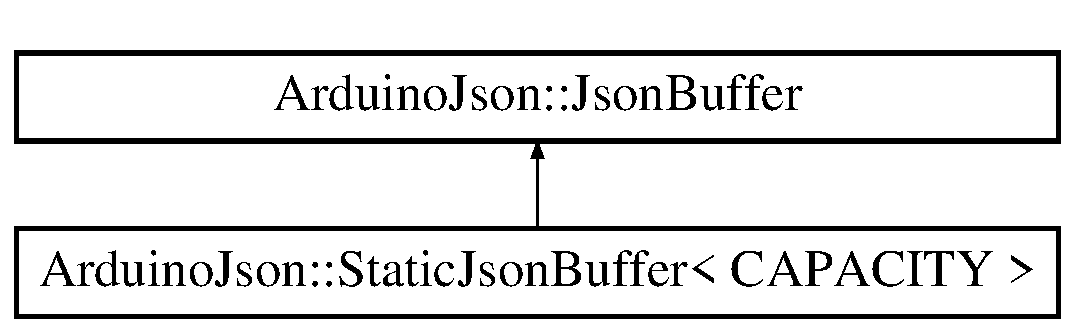
\includegraphics[height=2.000000cm]{class_arduino_json_1_1_static_json_buffer}
\end{center}
\end{figure}
\subsection*{Public Member Functions}
\begin{DoxyCompactItemize}
\item 
\hypertarget{class_arduino_json_1_1_static_json_buffer_ac7d04899629c73f8c8880725d16c4c7a}{}size\+\_\+t {\bfseries capacity} () const \label{class_arduino_json_1_1_static_json_buffer_ac7d04899629c73f8c8880725d16c4c7a}

\item 
\hypertarget{class_arduino_json_1_1_static_json_buffer_a58a2e4f0ecae55e0f74a67ed6084873c}{}size\+\_\+t {\bfseries size} () const \label{class_arduino_json_1_1_static_json_buffer_a58a2e4f0ecae55e0f74a67ed6084873c}

\end{DoxyCompactItemize}
\subsection*{Protected Member Functions}
\begin{DoxyCompactItemize}
\item 
\hypertarget{class_arduino_json_1_1_static_json_buffer_ac8a52d27c9f466104283e13fbf081444}{}virtual void $\ast$ {\bfseries alloc} (size\+\_\+t bytes)\label{class_arduino_json_1_1_static_json_buffer_ac8a52d27c9f466104283e13fbf081444}

\end{DoxyCompactItemize}
\subsection*{Additional Inherited Members}


The documentation for this class was generated from the following file\+:\begin{DoxyCompactItemize}
\item 
Services/\+Arduino\+Json/include/\+Arduino\+Json/Static\+Json\+Buffer.\+hpp\end{DoxyCompactItemize}

\hypertarget{class_station_class}{}\section{Station\+Class Class Reference}
\label{class_station_class}\index{Station\+Class@{Station\+Class}}
Inheritance diagram for Station\+Class\+:\begin{figure}[H]
\begin{center}
\leavevmode
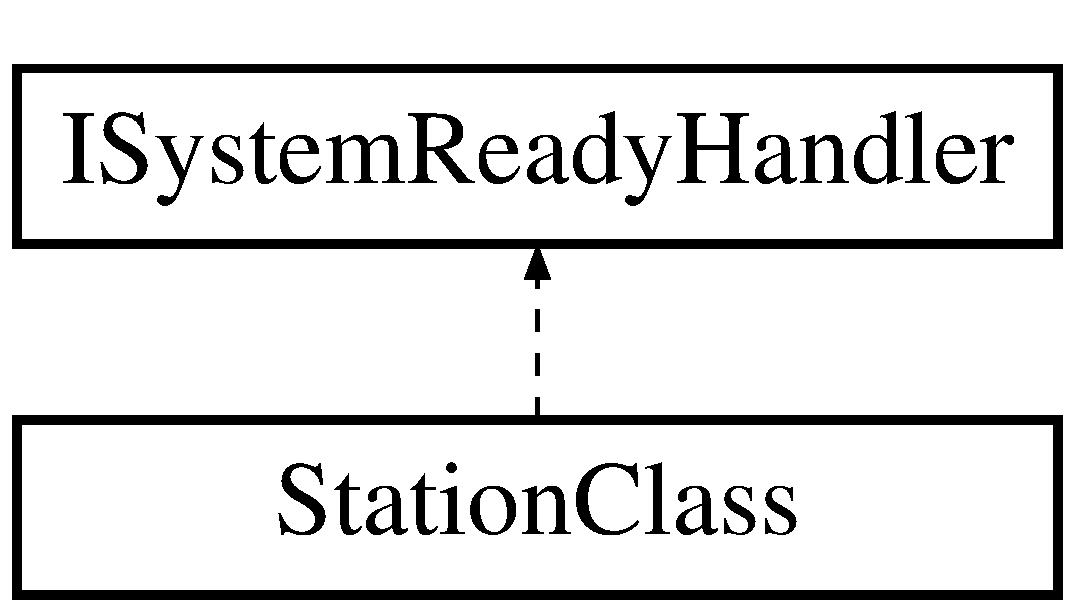
\includegraphics[height=2.000000cm]{class_station_class}
\end{center}
\end{figure}
\subsection*{Public Member Functions}
\begin{DoxyCompactItemize}
\item 
\hypertarget{class_station_class_a2d75f4b103a7b3716472d25cfb96721b}{}void {\bfseries enable} (bool enabled)\label{class_station_class_a2d75f4b103a7b3716472d25cfb96721b}

\item 
\hypertarget{class_station_class_a254b4e9bbd12fa349a0dc872f9129b87}{}bool {\bfseries is\+Enabled} ()\label{class_station_class_a254b4e9bbd12fa349a0dc872f9129b87}

\item 
\hypertarget{class_station_class_ab8f2acf6c2dbd5edd0fb227c62feb033}{}bool {\bfseries config} (String ssid, String password, bool auto\+Connect\+On\+Startup=true)\label{class_station_class_ab8f2acf6c2dbd5edd0fb227c62feb033}

\item 
\hypertarget{class_station_class_a9c0028f4b36957c6964adbfc95a4d5e3}{}bool {\bfseries is\+Connected} ()\label{class_station_class_a9c0028f4b36957c6964adbfc95a4d5e3}

\item 
\hypertarget{class_station_class_a68a06f1464ee0c3b7365e6914d269cca}{}bool {\bfseries is\+Connection\+Failed} ()\label{class_station_class_a68a06f1464ee0c3b7365e6914d269cca}

\item 
\hypertarget{class_station_class_abe754978b682adcae119b4ea0f762f8b}{}E\+Station\+Connection\+Status {\bfseries get\+Connection\+Status} ()\label{class_station_class_abe754978b682adcae119b4ea0f762f8b}

\item 
\hypertarget{class_station_class_a4a8fdbba05fa3343577471f6070adac3}{}const char $\ast$ {\bfseries get\+Connection\+Status\+Name} ()\label{class_station_class_a4a8fdbba05fa3343577471f6070adac3}

\item 
\hypertarget{class_station_class_affe9ad2f57b898551ede57c571c164df}{}bool {\bfseries is\+Enabled\+D\+H\+C\+P} ()\label{class_station_class_affe9ad2f57b898551ede57c571c164df}

\item 
\hypertarget{class_station_class_a828cf12352dce3e6dbddf656f2c55ca3}{}void {\bfseries enable\+D\+H\+C\+P} (bool enable)\label{class_station_class_a828cf12352dce3e6dbddf656f2c55ca3}

\item 
\hypertarget{class_station_class_a25875fc23dbeb4bc7c9a1a5f7fb76412}{}\hyperlink{class_i_p_address}{I\+P\+Address} {\bfseries get\+I\+P} ()\label{class_station_class_a25875fc23dbeb4bc7c9a1a5f7fb76412}

\item 
\hypertarget{class_station_class_aa83979edcf377f51ad5c6a61395a1c30}{}String {\bfseries get\+M\+A\+C} ()\label{class_station_class_aa83979edcf377f51ad5c6a61395a1c30}

\item 
\hypertarget{class_station_class_abd8b97163f6bf4dd3f0e372dfb464a37}{}\hyperlink{class_i_p_address}{I\+P\+Address} {\bfseries get\+Network\+Mask} ()\label{class_station_class_abd8b97163f6bf4dd3f0e372dfb464a37}

\item 
\hypertarget{class_station_class_a3b47d30a2dc3f191986a53a0188da4f4}{}\hyperlink{class_i_p_address}{I\+P\+Address} {\bfseries get\+Network\+Gateway} ()\label{class_station_class_a3b47d30a2dc3f191986a53a0188da4f4}

\item 
\hypertarget{class_station_class_a1a00baaffe6a6fe057c83a8074963963}{}bool {\bfseries set\+I\+P} (\hyperlink{class_i_p_address}{I\+P\+Address} address)\label{class_station_class_a1a00baaffe6a6fe057c83a8074963963}

\item 
\hypertarget{class_station_class_ad7419d830a45e093079ddad59e7b8577}{}bool {\bfseries set\+I\+P} (\hyperlink{class_i_p_address}{I\+P\+Address} address, \hyperlink{class_i_p_address}{I\+P\+Address} netmask, \hyperlink{class_i_p_address}{I\+P\+Address} gateway)\label{class_station_class_ad7419d830a45e093079ddad59e7b8577}

\item 
\hypertarget{class_station_class_ad15b66f03da67d5f3e0fe277f19b20a9}{}String {\bfseries get\+S\+S\+I\+D} ()\label{class_station_class_ad15b66f03da67d5f3e0fe277f19b20a9}

\item 
\hypertarget{class_station_class_a85c971fbafdcde8f1c77bb581319e2f2}{}String {\bfseries get\+Password} ()\label{class_station_class_a85c971fbafdcde8f1c77bb581319e2f2}

\item 
\hypertarget{class_station_class_a482f6a13867a91e3c1c1679dd333bfe9}{}bool {\bfseries start\+Scan} (Scan\+Completed\+Callback scan\+Completed)\label{class_station_class_a482f6a13867a91e3c1c1679dd333bfe9}

\item 
\hypertarget{class_station_class_a980dd3a0a1226eb840fa38a0f47fb522}{}void {\bfseries wait\+Connection} (Connection\+Callback successful\+Connected)\label{class_station_class_a980dd3a0a1226eb840fa38a0f47fb522}

\item 
\hypertarget{class_station_class_ac311ec6565c7cb40e7dfd3fd4ee1def3}{}void {\bfseries wait\+Connection} (Connection\+Callback successful\+Connected, int seconds\+Time\+Out, Connection\+Callback connection\+Not\+Established)\label{class_station_class_ac311ec6565c7cb40e7dfd3fd4ee1def3}

\end{DoxyCompactItemize}
\subsection*{Protected Member Functions}
\begin{DoxyCompactItemize}
\item 
\hypertarget{class_station_class_aff302d5d7f1d731cb10bbdd4318a9c6a}{}virtual void {\bfseries on\+System\+Ready} ()\label{class_station_class_aff302d5d7f1d731cb10bbdd4318a9c6a}

\item 
\hypertarget{class_station_class_ac42c43d86c9012c57cee313edef1dce1}{}void {\bfseries internal\+Check\+Connection} ()\label{class_station_class_ac42c43d86c9012c57cee313edef1dce1}

\end{DoxyCompactItemize}
\subsection*{Static Protected Member Functions}
\begin{DoxyCompactItemize}
\item 
\hypertarget{class_station_class_a14c0e92fdddbd4a704e0fcd6e7eb12ef}{}static void {\bfseries static\+Scan\+Completed} (void $\ast$arg, S\+T\+A\+T\+U\+S status)\label{class_station_class_a14c0e92fdddbd4a704e0fcd6e7eb12ef}

\item 
\hypertarget{class_station_class_af8d5ea5e2204a1894425ace25a5db8e4}{}static void {\bfseries static\+Check\+Connection} ()\label{class_station_class_af8d5ea5e2204a1894425ace25a5db8e4}

\end{DoxyCompactItemize}


The documentation for this class was generated from the following files\+:\begin{DoxyCompactItemize}
\item 
Sming\+Core/\+Platform/Station.\+h\item 
Sming\+Core/\+Platform/Station.\+cpp\end{DoxyCompactItemize}

\hypertarget{struct_s_t_o_r_e___t_y_p_e_d_e_f___a_t_t_r}{}\section{S\+T\+O\+R\+E\+\_\+\+T\+Y\+P\+E\+D\+E\+F\+\_\+\+A\+T\+T\+R Struct Reference}
\label{struct_s_t_o_r_e___t_y_p_e_d_e_f___a_t_t_r}\index{S\+T\+O\+R\+E\+\_\+\+T\+Y\+P\+E\+D\+E\+F\+\_\+\+A\+T\+T\+R@{S\+T\+O\+R\+E\+\_\+\+T\+Y\+P\+E\+D\+E\+F\+\_\+\+A\+T\+T\+R}}
\subsection*{Public Types}
\begin{DoxyCompactItemize}
\item 
\hypertarget{struct_s_t_o_r_e___t_y_p_e_d_e_f___a_t_t_r_a78785f3b323604217b18de2dfeda2a51}{}enum \{ {\bfseries M\+O\+D\+E\+\_\+\+Q\+I\+O} = 0, 
{\bfseries M\+O\+D\+E\+\_\+\+Q\+O\+U\+T} = 1, 
{\bfseries M\+O\+D\+E\+\_\+\+D\+I\+O} = 2, 
{\bfseries M\+O\+D\+E\+\_\+\+D\+O\+U\+T} = 15
 \}\label{struct_s_t_o_r_e___t_y_p_e_d_e_f___a_t_t_r_a78785f3b323604217b18de2dfeda2a51}

\item 
\hypertarget{struct_s_t_o_r_e___t_y_p_e_d_e_f___a_t_t_r_a500a52952a5cc52a56faae2de585bb66}{}enum \{ {\bfseries S\+P\+E\+E\+D\+\_\+40\+M\+H\+Z} = 0, 
{\bfseries S\+P\+E\+E\+D\+\_\+26\+M\+H\+Z} = 1, 
{\bfseries S\+P\+E\+E\+D\+\_\+20\+M\+H\+Z} = 2, 
{\bfseries S\+P\+E\+E\+D\+\_\+80\+M\+H\+Z} = 15
 \}\label{struct_s_t_o_r_e___t_y_p_e_d_e_f___a_t_t_r_a500a52952a5cc52a56faae2de585bb66}

\item 
\hypertarget{struct_s_t_o_r_e___t_y_p_e_d_e_f___a_t_t_r_af04d6fca2bc0f363d944bd8a33f83f72}{}enum \{ \\*
{\bfseries S\+I\+Z\+E\+\_\+4\+M\+B\+I\+T} = 0, 
{\bfseries S\+I\+Z\+E\+\_\+2\+M\+B\+I\+T} = 1, 
{\bfseries S\+I\+Z\+E\+\_\+8\+M\+B\+I\+T} = 2, 
{\bfseries S\+I\+Z\+E\+\_\+16\+M\+B\+I\+T} = 3, 
\\*
{\bfseries S\+I\+Z\+E\+\_\+32\+M\+B\+I\+T} = 4
 \}\label{struct_s_t_o_r_e___t_y_p_e_d_e_f___a_t_t_r_af04d6fca2bc0f363d944bd8a33f83f72}

\end{DoxyCompactItemize}
\subsection*{Public Attributes}
\begin{DoxyCompactItemize}
\item 
\hypertarget{struct_s_t_o_r_e___t_y_p_e_d_e_f___a_t_t_r_a4baee634765e402525cdd5a7533aa610}{}uint8\+\_\+t {\bfseries unknown0}\label{struct_s_t_o_r_e___t_y_p_e_d_e_f___a_t_t_r_a4baee634765e402525cdd5a7533aa610}

\item 
\hypertarget{struct_s_t_o_r_e___t_y_p_e_d_e_f___a_t_t_r_a43c9f263daf7fc85ce959a9f03797c00}{}uint8\+\_\+t {\bfseries unknown1}\label{struct_s_t_o_r_e___t_y_p_e_d_e_f___a_t_t_r_a43c9f263daf7fc85ce959a9f03797c00}

\item 
\hypertarget{struct_s_t_o_r_e___t_y_p_e_d_e_f___a_t_t_r_ac0765c6b523f6570a36c519d4712898d}{}enum S\+T\+O\+R\+E\+\_\+\+T\+Y\+P\+E\+D\+E\+F\+\_\+\+A\+T\+T\+R\+:: \{ ... \}  {\bfseries mode}\label{struct_s_t_o_r_e___t_y_p_e_d_e_f___a_t_t_r_ac0765c6b523f6570a36c519d4712898d}

\item 
\hypertarget{struct_s_t_o_r_e___t_y_p_e_d_e_f___a_t_t_r_a21d923b01e2201ea767e2b9912557b31}{}enum S\+T\+O\+R\+E\+\_\+\+T\+Y\+P\+E\+D\+E\+F\+\_\+\+A\+T\+T\+R\+:: \{ ... \}  {\bfseries speed}\label{struct_s_t_o_r_e___t_y_p_e_d_e_f___a_t_t_r_a21d923b01e2201ea767e2b9912557b31}

\item 
\hypertarget{struct_s_t_o_r_e___t_y_p_e_d_e_f___a_t_t_r_a669b37aa21615e1ccd16145569b095e1}{}enum S\+T\+O\+R\+E\+\_\+\+T\+Y\+P\+E\+D\+E\+F\+\_\+\+A\+T\+T\+R\+:: \{ ... \}  {\bfseries size}\label{struct_s_t_o_r_e___t_y_p_e_d_e_f___a_t_t_r_a669b37aa21615e1ccd16145569b095e1}

\end{DoxyCompactItemize}


The documentation for this struct was generated from the following file\+:\begin{DoxyCompactItemize}
\item 
system/flashmem.\+h\end{DoxyCompactItemize}

\hypertarget{class_stream}{}\section{Stream Class Reference}
\label{class_stream}\index{Stream@{Stream}}
Inheritance diagram for Stream\+:\begin{figure}[H]
\begin{center}
\leavevmode
\includegraphics[height=3.000000cm]{class_stream}
\end{center}
\end{figure}
\subsection*{Public Member Functions}
\begin{DoxyCompactItemize}
\item 
\hypertarget{class_stream_a9c98a763395005c08ce95afb2f06c7b1}{}virtual int {\bfseries available} ()=0\label{class_stream_a9c98a763395005c08ce95afb2f06c7b1}

\item 
\hypertarget{class_stream_a30c3c212ec6ea67277a708c5ea2501a5}{}virtual int {\bfseries peek} ()=0\label{class_stream_a30c3c212ec6ea67277a708c5ea2501a5}

\item 
\hypertarget{class_stream_aea5dee9fcb038148515b7c9212d38dc0}{}virtual int {\bfseries read} ()=0\label{class_stream_aea5dee9fcb038148515b7c9212d38dc0}

\item 
\hypertarget{class_stream_aa3ef2c34f152a0b2ea8de9139b9461da}{}virtual void {\bfseries flush} ()=0\label{class_stream_aa3ef2c34f152a0b2ea8de9139b9461da}

\item 
\hypertarget{class_stream_a851dd6dc74d52389de04f99648478db5}{}void {\bfseries set\+Timeout} (unsigned long timeout)\label{class_stream_a851dd6dc74d52389de04f99648478db5}

\item 
\hypertarget{class_stream_a4bab30ccd324efd461dee46a2339f673}{}bool {\bfseries find} (char $\ast$target)\label{class_stream_a4bab30ccd324efd461dee46a2339f673}

\item 
\hypertarget{class_stream_ad851401f2318cdb1de05707e021b81d9}{}bool {\bfseries find} (char $\ast$target, size\+\_\+t length)\label{class_stream_ad851401f2318cdb1de05707e021b81d9}

\item 
\hypertarget{class_stream_ad1f5f6600832396fb38a897baf4de35b}{}bool {\bfseries find\+Until} (char $\ast$target, char $\ast$terminator)\label{class_stream_ad1f5f6600832396fb38a897baf4de35b}

\item 
\hypertarget{class_stream_a3a9497de614792103ab8cb4759e01a69}{}bool {\bfseries find\+Until} (char $\ast$target, size\+\_\+t target\+Len, char $\ast$terminate, size\+\_\+t term\+Len)\label{class_stream_a3a9497de614792103ab8cb4759e01a69}

\item 
\hypertarget{class_stream_a497ffcbcb4d5bb889a8fde487bcc1b98}{}long {\bfseries parse\+Int} ()\label{class_stream_a497ffcbcb4d5bb889a8fde487bcc1b98}

\item 
\hypertarget{class_stream_a5e5a0cc11eb586d89dcb7fa8e53a87e8}{}float {\bfseries parse\+Float} ()\label{class_stream_a5e5a0cc11eb586d89dcb7fa8e53a87e8}

\item 
\hypertarget{class_stream_a45fd1336a323ea83b16e8507055f44ea}{}size\+\_\+t {\bfseries read\+Bytes} (char $\ast$buffer, size\+\_\+t length)\label{class_stream_a45fd1336a323ea83b16e8507055f44ea}

\item 
\hypertarget{class_stream_af84672a4fb2620466958d3118d4fea00}{}size\+\_\+t {\bfseries read\+Bytes\+Until} (char terminator, char $\ast$buffer, size\+\_\+t length)\label{class_stream_af84672a4fb2620466958d3118d4fea00}

\item 
\hypertarget{class_stream_a1c60bdda2b65d78e5a1362d51b856c5a}{}String {\bfseries read\+String} ()\label{class_stream_a1c60bdda2b65d78e5a1362d51b856c5a}

\item 
\hypertarget{class_stream_a6a409da87c552909260d8cc428c5ca70}{}String {\bfseries read\+String\+Until} (char terminator)\label{class_stream_a6a409da87c552909260d8cc428c5ca70}

\end{DoxyCompactItemize}
\subsection*{Protected Member Functions}
\begin{DoxyCompactItemize}
\item 
\hypertarget{class_stream_a416a0ada5ed3c9d27f1e72c7d73f0aa1}{}int {\bfseries timed\+Read} ()\label{class_stream_a416a0ada5ed3c9d27f1e72c7d73f0aa1}

\item 
\hypertarget{class_stream_ae326bf60a3c5276836526710871046fe}{}int {\bfseries timed\+Peek} ()\label{class_stream_ae326bf60a3c5276836526710871046fe}

\item 
\hypertarget{class_stream_ab31c533ddc422c8d8df07986e5920534}{}int {\bfseries peek\+Next\+Digit} ()\label{class_stream_ab31c533ddc422c8d8df07986e5920534}

\item 
\hypertarget{class_stream_a4578615defade6c4ce7daeb6578bb62d}{}long {\bfseries parse\+Int} (char skip\+Char)\label{class_stream_a4578615defade6c4ce7daeb6578bb62d}

\item 
\hypertarget{class_stream_a14a98cdbb166008f25dd044d836b1864}{}float {\bfseries parse\+Float} (char skip\+Char)\label{class_stream_a14a98cdbb166008f25dd044d836b1864}

\end{DoxyCompactItemize}
\subsection*{Protected Attributes}
\begin{DoxyCompactItemize}
\item 
\hypertarget{class_stream_aae48f1a926d2e82a452f2c75af0c6a29}{}unsigned long {\bfseries \+\_\+timeout}\label{class_stream_aae48f1a926d2e82a452f2c75af0c6a29}

\item 
\hypertarget{class_stream_abf61d2006d28d18f2e028285a323fe5a}{}unsigned long {\bfseries \+\_\+start\+Millis}\label{class_stream_abf61d2006d28d18f2e028285a323fe5a}

\end{DoxyCompactItemize}


The documentation for this class was generated from the following files\+:\begin{DoxyCompactItemize}
\item 
Wiring/Stream.\+h\item 
Wiring/Stream.\+cpp\end{DoxyCompactItemize}

\hypertarget{class_arduino_json_1_1_internals_1_1_string_builder}{}\section{Arduino\+Json\+:\+:Internals\+:\+:String\+Builder Class Reference}
\label{class_arduino_json_1_1_internals_1_1_string_builder}\index{Arduino\+Json\+::\+Internals\+::\+String\+Builder@{Arduino\+Json\+::\+Internals\+::\+String\+Builder}}
Inheritance diagram for Arduino\+Json\+:\+:Internals\+:\+:String\+Builder\+:\begin{figure}[H]
\begin{center}
\leavevmode
\includegraphics[height=2.000000cm]{class_arduino_json_1_1_internals_1_1_string_builder}
\end{center}
\end{figure}
\subsection*{Public Member Functions}
\begin{DoxyCompactItemize}
\item 
\hypertarget{class_arduino_json_1_1_internals_1_1_string_builder_a983e5b4722cdb62b232cce28ff775ac7}{}{\bfseries String\+Builder} (char $\ast$buf, int size)\label{class_arduino_json_1_1_internals_1_1_string_builder_a983e5b4722cdb62b232cce28ff775ac7}

\item 
\hypertarget{class_arduino_json_1_1_internals_1_1_string_builder_a2ce8b059fd24afd6174adb010555603e}{}virtual size\+\_\+t {\bfseries write} (uint8\+\_\+t c)\label{class_arduino_json_1_1_internals_1_1_string_builder_a2ce8b059fd24afd6174adb010555603e}

\end{DoxyCompactItemize}


The documentation for this class was generated from the following files\+:\begin{DoxyCompactItemize}
\item 
Services/\+Arduino\+Json/include/\+Arduino\+Json/\+Internals/String\+Builder.\+hpp\item 
Services/\+Arduino\+Json/src/\+Internals/String\+Builder.\+cpp\end{DoxyCompactItemize}

\hypertarget{structsys__timeo}{}\section{sys\+\_\+timeo Struct Reference}
\label{structsys__timeo}\index{sys\+\_\+timeo@{sys\+\_\+timeo}}
\subsection*{Public Attributes}
\begin{DoxyCompactItemize}
\item 
\hypertarget{structsys__timeo_addfc1875758f06d6036f5dda30beed9e}{}struct \hyperlink{structsys__timeo}{sys\+\_\+timeo} $\ast$ {\bfseries next}\label{structsys__timeo_addfc1875758f06d6036f5dda30beed9e}

\item 
\hypertarget{structsys__timeo_a7641719a0ce0daec85e86f188f03bca1}{}u32\+\_\+t {\bfseries time}\label{structsys__timeo_a7641719a0ce0daec85e86f188f03bca1}

\item 
\hypertarget{structsys__timeo_a483e9c13d60e0adf6731869daa3e8b4d}{}sys\+\_\+timeout\+\_\+handler {\bfseries h}\label{structsys__timeo_a483e9c13d60e0adf6731869daa3e8b4d}

\item 
\hypertarget{structsys__timeo_a74e07a9d80232319984ee3112e91eef3}{}void $\ast$ {\bfseries arg}\label{structsys__timeo_a74e07a9d80232319984ee3112e91eef3}

\end{DoxyCompactItemize}


The documentation for this struct was generated from the following file\+:\begin{DoxyCompactItemize}
\item 
system/include/lwip/timers.\+h\end{DoxyCompactItemize}

\hypertarget{class_system_class}{}\section{System\+Class Class Reference}
\label{class_system_class}\index{System\+Class@{System\+Class}}
\subsection*{Public Member Functions}
\begin{DoxyCompactItemize}
\item 
\hypertarget{class_system_class_a6f76530665629e2a2d0246fb63af9696}{}void {\bfseries initialize} ()\label{class_system_class_a6f76530665629e2a2d0246fb63af9696}

\item 
\hypertarget{class_system_class_a79a7cb0d48d4f5ae35722cfff45aa454}{}bool {\bfseries is\+Ready} ()\label{class_system_class_a79a7cb0d48d4f5ae35722cfff45aa454}

\item 
\hypertarget{class_system_class_a5f72899b23c49108b7cba82717e4246d}{}void {\bfseries restart} ()\label{class_system_class_a5f72899b23c49108b7cba82717e4246d}

\item 
\hypertarget{class_system_class_a820222ab31f457872e7bc645e998024f}{}void {\bfseries set\+Cpu\+Frequency} (Cpu\+Frequency freq)\label{class_system_class_a820222ab31f457872e7bc645e998024f}

\item 
\hypertarget{class_system_class_a4ee160d3a5da1913480bfee8c42df41a}{}Cpu\+Frequency {\bfseries get\+Cpu\+Frequency} ()\label{class_system_class_a4ee160d3a5da1913480bfee8c42df41a}

\item 
\hypertarget{class_system_class_a15eb21125083b655bb83f7dbd47f0987}{}bool {\bfseries deep\+Sleep} (uint32 time\+Milliseconds, Deep\+Sleep\+Options options=e\+D\+S\+O\+\_\+\+R\+F\+\_\+\+C\+A\+L\+\_\+\+B\+Y\+\_\+\+I\+N\+I\+T\+\_\+\+D\+A\+T\+A)\label{class_system_class_a15eb21125083b655bb83f7dbd47f0987}

\item 
\hypertarget{class_system_class_a4975b9d61d16329fe5cdbf71a06f8a79}{}void {\bfseries on\+Ready} (System\+Ready\+Callback ready\+Handler)\label{class_system_class_a4975b9d61d16329fe5cdbf71a06f8a79}

\item 
\hypertarget{class_system_class_a71e2a19d176b06ed76394b771a2cb487}{}void {\bfseries on\+Ready} (\hyperlink{class_i_system_ready_handler}{I\+System\+Ready\+Handler} $\ast$ready\+Handler)\label{class_system_class_a71e2a19d176b06ed76394b771a2cb487}

\item 
\hypertarget{class_system_class_a7dcef7d03311a356b501b6864a0b39ff}{}void {\bfseries apply\+Firmware\+Update} (uint32\+\_\+t read\+Flash\+Offset, uint32\+\_\+t target\+Flash\+Offset, int firmware\+Size)\label{class_system_class_a7dcef7d03311a356b501b6864a0b39ff}

\end{DoxyCompactItemize}


The documentation for this class was generated from the following files\+:\begin{DoxyCompactItemize}
\item 
Sming\+Core/\+Platform/System.\+h\item 
Sming\+Core/\+Platform/System.\+cpp\end{DoxyCompactItemize}

\hypertarget{class_system_clock_class}{}\section{System\+Clock\+Class Class Reference}
\label{class_system_clock_class}\index{System\+Clock\+Class@{System\+Clock\+Class}}
\subsection*{Public Member Functions}
\begin{DoxyCompactItemize}
\item 
\hypertarget{class_system_clock_class_afd37e409805ad1539a41078530111f8c}{}\hyperlink{class_date_time}{Date\+Time} {\bfseries now} (e\+Sys\+Clock\+Time time\+Type=e\+S\+C\+Local)\label{class_system_clock_class_afd37e409805ad1539a41078530111f8c}

\item 
\hypertarget{class_system_clock_class_af35d19f7fc85bcd762527d283c9cc6c5}{}void {\bfseries set\+Time} (time\+\_\+t time, e\+Sys\+Clock\+Time time\+Type=e\+S\+C\+Local)\label{class_system_clock_class_af35d19f7fc85bcd762527d283c9cc6c5}

\item 
\hypertarget{class_system_clock_class_a14d266686be92b56ea1896a3da4320ca}{}String {\bfseries get\+System\+Time\+String} (e\+Sys\+Clock\+Time time\+Type=e\+S\+C\+Local)\label{class_system_clock_class_a14d266686be92b56ea1896a3da4320ca}

\item 
\hypertarget{class_system_clock_class_a4bbd59de38bce5bf2d6585b5cfb81a27}{}bool {\bfseries set\+Timezone} (double req\+Timezone)\label{class_system_clock_class_a4bbd59de38bce5bf2d6585b5cfb81a27}

\item 
\hypertarget{class_system_clock_class_a0db5adecd4846623fbaad3c3fa1c21ff}{}void {\bfseries set\+Ntp\+Sync} (String req\+Server, int req\+Interval)\label{class_system_clock_class_a0db5adecd4846623fbaad3c3fa1c21ff}

\end{DoxyCompactItemize}
\subsection*{Public Attributes}
\begin{DoxyCompactItemize}
\item 
\hypertarget{class_system_clock_class_a8a6bf60237d8b83f2a068dbbc51acc53}{}\hyperlink{class_ntp_client}{Ntp\+Client} $\ast$ {\bfseries ntp\+Client} = nullptr\label{class_system_clock_class_a8a6bf60237d8b83f2a068dbbc51acc53}

\end{DoxyCompactItemize}


The documentation for this class was generated from the following files\+:\begin{DoxyCompactItemize}
\item 
Sming\+Core/System\+Clock.\+h\item 
Sming\+Core/System\+Clock.\+cpp\end{DoxyCompactItemize}

\hypertarget{class_tcp_client}{}\section{Tcp\+Client Class Reference}
\label{class_tcp_client}\index{Tcp\+Client@{Tcp\+Client}}
Inheritance diagram for Tcp\+Client\+:\begin{figure}[H]
\begin{center}
\leavevmode
\includegraphics[height=4.000000cm]{class_tcp_client}
\end{center}
\end{figure}
\subsection*{Public Member Functions}
\begin{DoxyCompactItemize}
\item 
\hypertarget{class_tcp_client_a4d2ba17936e3447c4e19984c1452f58c}{}{\bfseries Tcp\+Client} (bool auto\+Destruct)\label{class_tcp_client_a4d2ba17936e3447c4e19984c1452f58c}

\item 
\hypertarget{class_tcp_client_a497b51d3af4d908bd5f8fc834406d958}{}{\bfseries Tcp\+Client} (tcp\+\_\+pcb $\ast$client\+Tcp, \hyperlink{class_delegate}{Tcp\+Client\+Data\+Callback} client\+Receive, bool auto\+Destruct)\label{class_tcp_client_a497b51d3af4d908bd5f8fc834406d958}

\item 
\hypertarget{class_tcp_client_a917bbc3e31bbe21d8559c10239c57e93}{}{\bfseries Tcp\+Client} (\hyperlink{class_delegate}{Tcp\+Client\+Bool\+Callback} on\+Completed, \hyperlink{class_delegate}{Tcp\+Client\+Event\+Callback} on\+Ready\+To\+Send, \hyperlink{class_delegate}{Tcp\+Client\+Data\+Callback} on\+Receive=N\+U\+L\+L)\label{class_tcp_client_a917bbc3e31bbe21d8559c10239c57e93}

\item 
\hypertarget{class_tcp_client_a07f2ee5c3af559cdcc907c2966f23d2b}{}{\bfseries Tcp\+Client} (\hyperlink{class_delegate}{Tcp\+Client\+Bool\+Callback} on\+Completed, \hyperlink{class_delegate}{Tcp\+Client\+Data\+Callback} on\+Receive=N\+U\+L\+L)\label{class_tcp_client_a07f2ee5c3af559cdcc907c2966f23d2b}

\item 
\hypertarget{class_tcp_client_aac792f1ec97d83a5d585b3d8d2c37d9a}{}{\bfseries Tcp\+Client} (\hyperlink{class_delegate}{Tcp\+Client\+Data\+Callback} on\+Receive)\label{class_tcp_client_aac792f1ec97d83a5d585b3d8d2c37d9a}

\item 
\hypertarget{class_tcp_client_afd0490a4bf9a16b3609828d61b51b36f}{}virtual bool {\bfseries connect} (String server, int port)\label{class_tcp_client_afd0490a4bf9a16b3609828d61b51b36f}

\item 
\hypertarget{class_tcp_client_a50f33d7a069d02a419c1280f665b89ad}{}virtual bool {\bfseries connect} (\hyperlink{class_i_p_address}{I\+P\+Address} addr, uint16\+\_\+t port)\label{class_tcp_client_a50f33d7a069d02a419c1280f665b89ad}

\item 
\hypertarget{class_tcp_client_a1ee082bbca3927811bbe2c0aa75386c4}{}virtual void {\bfseries close} ()\label{class_tcp_client_a1ee082bbca3927811bbe2c0aa75386c4}

\item 
\hypertarget{class_tcp_client_a38bf30a25fe74a70ef874bb2524a6da3}{}bool {\bfseries send} (const char $\ast$data, uint8\+\_\+t len, bool force\+Close\+After\+Sent=false)\label{class_tcp_client_a38bf30a25fe74a70ef874bb2524a6da3}

\item 
\hypertarget{class_tcp_client_a08a4c755e8dab2b3761a56ac8386e41b}{}bool {\bfseries send\+String} (String data, bool force\+Close\+After\+Sent=false)\label{class_tcp_client_a08a4c755e8dab2b3761a56ac8386e41b}

\item 
\hypertarget{class_tcp_client_af97510bea711663fbe4803829561c968}{}\+\_\+\+\_\+forceinline bool {\bfseries is\+Processing} ()\label{class_tcp_client_af97510bea711663fbe4803829561c968}

\item 
\hypertarget{class_tcp_client_a39adb717bf57c16fcd6496752bda510a}{}\+\_\+\+\_\+forceinline Tcp\+Client\+State {\bfseries get\+State} ()\label{class_tcp_client_a39adb717bf57c16fcd6496752bda510a}

\end{DoxyCompactItemize}
\subsection*{Protected Member Functions}
\begin{DoxyCompactItemize}
\item 
\hypertarget{class_tcp_client_a45b8fb12ee004796d53ddbed19a18f47}{}virtual err\+\_\+t {\bfseries on\+Connected} (err\+\_\+t err)\label{class_tcp_client_a45b8fb12ee004796d53ddbed19a18f47}

\item 
\hypertarget{class_tcp_client_aa756d90a9f145de249073adf51326a35}{}virtual err\+\_\+t {\bfseries on\+Receive} (\hyperlink{structpbuf}{pbuf} $\ast$buf)\label{class_tcp_client_aa756d90a9f145de249073adf51326a35}

\item 
\hypertarget{class_tcp_client_aa5636a7fbd1272a72fee443c30e450a8}{}virtual err\+\_\+t {\bfseries on\+Sent} (uint16\+\_\+t len)\label{class_tcp_client_aa5636a7fbd1272a72fee443c30e450a8}

\item 
\hypertarget{class_tcp_client_afeb67a00dabb644f1e7868e4605031b5}{}virtual void {\bfseries on\+Error} (err\+\_\+t err)\label{class_tcp_client_afeb67a00dabb644f1e7868e4605031b5}

\item 
\hypertarget{class_tcp_client_aea9b23efa5fc8b975b509344c52fa8b9}{}virtual void {\bfseries on\+Ready\+To\+Send\+Data} (Tcp\+Connection\+Event source\+Event)\label{class_tcp_client_aea9b23efa5fc8b975b509344c52fa8b9}

\item 
\hypertarget{class_tcp_client_ac36af0e7978a712b0833d40151f4ff85}{}virtual void {\bfseries on\+Finished} (Tcp\+Client\+State finish\+State)\label{class_tcp_client_ac36af0e7978a712b0833d40151f4ff85}

\item 
\hypertarget{class_tcp_client_a162be33aa3e851eb92ccd361f64c6706}{}void {\bfseries push\+Async\+Part} ()\label{class_tcp_client_a162be33aa3e851eb92ccd361f64c6706}

\end{DoxyCompactItemize}
\subsection*{Additional Inherited Members}


The documentation for this class was generated from the following files\+:\begin{DoxyCompactItemize}
\item 
Sming\+Core/\+Network/Tcp\+Client.\+h\item 
Sming\+Core/\+Network/Tcp\+Client.\+cpp\end{DoxyCompactItemize}

\hypertarget{class_tcp_connection}{}\section{Tcp\+Connection Class Reference}
\label{class_tcp_connection}\index{Tcp\+Connection@{Tcp\+Connection}}
Inheritance diagram for Tcp\+Connection\+:\begin{figure}[H]
\begin{center}
\leavevmode
\includegraphics[height=1.917808cm]{class_tcp_connection}
\end{center}
\end{figure}
\subsection*{Public Member Functions}
\begin{DoxyCompactItemize}
\item 
\hypertarget{class_tcp_connection_a6cda2bd2cfedc12cd0fcfbc47df5cec0}{}{\bfseries Tcp\+Connection} (bool auto\+Destruct)\label{class_tcp_connection_a6cda2bd2cfedc12cd0fcfbc47df5cec0}

\item 
\hypertarget{class_tcp_connection_a936b499d010ead10fdcf73aa4b50ad00}{}{\bfseries Tcp\+Connection} (tcp\+\_\+pcb $\ast$connection, bool auto\+Destruct)\label{class_tcp_connection_a936b499d010ead10fdcf73aa4b50ad00}

\item 
\hypertarget{class_tcp_connection_a349069802d8743ab29024b755424773e}{}virtual bool {\bfseries connect} (String server, int port)\label{class_tcp_connection_a349069802d8743ab29024b755424773e}

\item 
\hypertarget{class_tcp_connection_ae7b39dfc9d8627c7782f6e434058fff1}{}virtual bool {\bfseries connect} (\hyperlink{class_i_p_address}{I\+P\+Address} addr, uint16\+\_\+t port)\label{class_tcp_connection_ae7b39dfc9d8627c7782f6e434058fff1}

\item 
\hypertarget{class_tcp_connection_a19d2aae1831da848f13f8fc6101e40ee}{}virtual void {\bfseries close} ()\label{class_tcp_connection_a19d2aae1831da848f13f8fc6101e40ee}

\item 
\hypertarget{class_tcp_connection_a3d6b422ffcb3718c74477d9140288edb}{}int {\bfseries write\+String} (const char $\ast$data, uint8\+\_\+t apiflags=T\+C\+P\+\_\+\+W\+R\+I\+T\+E\+\_\+\+F\+L\+A\+G\+\_\+\+C\+O\+P\+Y)\label{class_tcp_connection_a3d6b422ffcb3718c74477d9140288edb}

\item 
\hypertarget{class_tcp_connection_a5165ea409d9d30a227f2aa76a0669948}{}int {\bfseries write\+String} (const String data, uint8\+\_\+t apiflags=T\+C\+P\+\_\+\+W\+R\+I\+T\+E\+\_\+\+F\+L\+A\+G\+\_\+\+C\+O\+P\+Y)\label{class_tcp_connection_a5165ea409d9d30a227f2aa76a0669948}

\item 
\hypertarget{class_tcp_connection_a3dca7b769bc01da34f881748de98d3f9}{}virtual int {\bfseries write} (const char $\ast$data, int len, uint8\+\_\+t apiflags=T\+C\+P\+\_\+\+W\+R\+I\+T\+E\+\_\+\+F\+L\+A\+G\+\_\+\+C\+O\+P\+Y)\label{class_tcp_connection_a3dca7b769bc01da34f881748de98d3f9}

\item 
\hypertarget{class_tcp_connection_a59ef4474eb3d65f8b1f1e21e0f3f3c25}{}int {\bfseries write} (\hyperlink{class_i_data_source_stream}{I\+Data\+Source\+Stream} $\ast$stream)\label{class_tcp_connection_a59ef4474eb3d65f8b1f1e21e0f3f3c25}

\item 
\hypertarget{class_tcp_connection_ab8d1467ac2d76882be7ec74f0aa0e1bf}{}\+\_\+\+\_\+forceinline uint16\+\_\+t {\bfseries get\+Available\+Write\+Size} ()\label{class_tcp_connection_ab8d1467ac2d76882be7ec74f0aa0e1bf}

\item 
\hypertarget{class_tcp_connection_aaaa45b0c9a0b26df7f8ca79697785114}{}void {\bfseries flush} ()\label{class_tcp_connection_aaaa45b0c9a0b26df7f8ca79697785114}

\item 
\hypertarget{class_tcp_connection_a3d01ef17727966d8d63e6f35a2a0fd14}{}void {\bfseries set\+Time\+Out} (uint16\+\_\+t wait\+Time\+Out)\label{class_tcp_connection_a3d01ef17727966d8d63e6f35a2a0fd14}

\item 
\hypertarget{class_tcp_connection_a333a64364cd35ef53615bd52b9918825}{}\hyperlink{class_i_p_address}{I\+P\+Address} {\bfseries get\+Remote\+Ip} ()\label{class_tcp_connection_a333a64364cd35ef53615bd52b9918825}

\item 
\hypertarget{class_tcp_connection_ad6fedbbb90a1147bde5b143fd8fdde6f}{}uint16\+\_\+t {\bfseries get\+Remote\+Port} ()\label{class_tcp_connection_ad6fedbbb90a1147bde5b143fd8fdde6f}

\end{DoxyCompactItemize}
\subsection*{Protected Member Functions}
\begin{DoxyCompactItemize}
\item 
\hypertarget{class_tcp_connection_a7799e1af79b2a94e0ef2f22ec35f84e4}{}bool {\bfseries intternal\+Tcp\+Connect} (\hyperlink{class_i_p_address}{I\+P\+Address} addr, uint16\+\_\+t port)\label{class_tcp_connection_a7799e1af79b2a94e0ef2f22ec35f84e4}

\item 
\hypertarget{class_tcp_connection_a3428bc222544c79ff0e78c0d41b9fa19}{}virtual err\+\_\+t {\bfseries on\+Connected} (err\+\_\+t err)\label{class_tcp_connection_a3428bc222544c79ff0e78c0d41b9fa19}

\item 
\hypertarget{class_tcp_connection_a393ef974edeac2c7ae2567a3316ded71}{}virtual err\+\_\+t {\bfseries on\+Receive} (\hyperlink{structpbuf}{pbuf} $\ast$buf)\label{class_tcp_connection_a393ef974edeac2c7ae2567a3316ded71}

\item 
\hypertarget{class_tcp_connection_a467b57cb414fcf3f4af31f9293cc157d}{}virtual err\+\_\+t {\bfseries on\+Sent} (uint16\+\_\+t len)\label{class_tcp_connection_a467b57cb414fcf3f4af31f9293cc157d}

\item 
\hypertarget{class_tcp_connection_a4f4f516d32911ca3fb0d32190ff24bbf}{}virtual err\+\_\+t {\bfseries on\+Poll} ()\label{class_tcp_connection_a4f4f516d32911ca3fb0d32190ff24bbf}

\item 
\hypertarget{class_tcp_connection_ab561bbbca2556644949994b5cae7ef81}{}virtual void {\bfseries on\+Error} (err\+\_\+t err)\label{class_tcp_connection_ab561bbbca2556644949994b5cae7ef81}

\item 
\hypertarget{class_tcp_connection_a763da2a7294bceee0f727b780856b252}{}virtual void {\bfseries on\+Ready\+To\+Send\+Data} (Tcp\+Connection\+Event source\+Event)\label{class_tcp_connection_a763da2a7294bceee0f727b780856b252}

\item 
\hypertarget{class_tcp_connection_adebe96bd5f3f5d2bc83f69fb7c7828c5}{}void {\bfseries initialize} (tcp\+\_\+pcb $\ast$pcb)\label{class_tcp_connection_adebe96bd5f3f5d2bc83f69fb7c7828c5}

\end{DoxyCompactItemize}
\subsection*{Static Protected Member Functions}
\begin{DoxyCompactItemize}
\item 
\hypertarget{class_tcp_connection_a2a4cb57a5feac6564230e207e9be583c}{}static err\+\_\+t {\bfseries static\+On\+Connected} (void $\ast$arg, tcp\+\_\+pcb $\ast$tcp, err\+\_\+t err)\label{class_tcp_connection_a2a4cb57a5feac6564230e207e9be583c}

\item 
\hypertarget{class_tcp_connection_a9a344b6bfd607d2c1b0131ef54e8f195}{}static err\+\_\+t {\bfseries static\+On\+Receive} (void $\ast$arg, tcp\+\_\+pcb $\ast$tcp, \hyperlink{structpbuf}{pbuf} $\ast$p, err\+\_\+t err)\label{class_tcp_connection_a9a344b6bfd607d2c1b0131ef54e8f195}

\item 
\hypertarget{class_tcp_connection_a49253c84f376a53a2b4bb74eb66b2e63}{}static err\+\_\+t {\bfseries static\+On\+Sent} (void $\ast$arg, tcp\+\_\+pcb $\ast$tcp, uint16\+\_\+t len)\label{class_tcp_connection_a49253c84f376a53a2b4bb74eb66b2e63}

\item 
\hypertarget{class_tcp_connection_a09675b3f46fd12a8de765f74fb5ccb0a}{}static err\+\_\+t {\bfseries static\+On\+Poll} (void $\ast$arg, tcp\+\_\+pcb $\ast$tcp)\label{class_tcp_connection_a09675b3f46fd12a8de765f74fb5ccb0a}

\item 
\hypertarget{class_tcp_connection_ac50d90859ccd3209640f9acfd0834b0b}{}static void {\bfseries static\+On\+Error} (void $\ast$arg, err\+\_\+t err)\label{class_tcp_connection_ac50d90859ccd3209640f9acfd0834b0b}

\item 
\hypertarget{class_tcp_connection_a92583d25ced7b447e9dd871da15d4644}{}static void {\bfseries static\+Dns\+Response} (const char $\ast$name, ip\+\_\+addr\+\_\+t $\ast$ipaddr, void $\ast$arg)\label{class_tcp_connection_a92583d25ced7b447e9dd871da15d4644}

\item 
\hypertarget{class_tcp_connection_a4a4fa5228dc736531c7eea389f6523b7}{}static void {\bfseries close\+Tcp\+Connection} (tcp\+\_\+pcb $\ast$tpcb)\label{class_tcp_connection_a4a4fa5228dc736531c7eea389f6523b7}

\end{DoxyCompactItemize}
\subsection*{Protected Attributes}
\begin{DoxyCompactItemize}
\item 
\hypertarget{class_tcp_connection_a601e019508b0071d0825908eaee0f58c}{}tcp\+\_\+pcb $\ast$ {\bfseries tcp}\label{class_tcp_connection_a601e019508b0071d0825908eaee0f58c}

\item 
\hypertarget{class_tcp_connection_a482c5afdb16d0a93c46a8b83da649254}{}uint16\+\_\+t {\bfseries sleep}\label{class_tcp_connection_a482c5afdb16d0a93c46a8b83da649254}

\item 
\hypertarget{class_tcp_connection_a3d11a5464ae92193779dafc650597fa2}{}uint16\+\_\+t {\bfseries time\+Out}\label{class_tcp_connection_a3d11a5464ae92193779dafc650597fa2}

\item 
\hypertarget{class_tcp_connection_a730b80fbbafb4ac92eda9b320ccf7bbf}{}bool {\bfseries can\+Send}\label{class_tcp_connection_a730b80fbbafb4ac92eda9b320ccf7bbf}

\item 
\hypertarget{class_tcp_connection_a56f9a3c4c74d221c29e07107384db1c1}{}bool {\bfseries auto\+Self\+Destruct}\label{class_tcp_connection_a56f9a3c4c74d221c29e07107384db1c1}

\end{DoxyCompactItemize}


The documentation for this class was generated from the following files\+:\begin{DoxyCompactItemize}
\item 
Sming\+Core/\+Network/Tcp\+Connection.\+h\item 
Sming\+Core/\+Network/Tcp\+Connection.\+cpp\end{DoxyCompactItemize}

\hypertarget{structtcpip__msg}{}\section{tcpip\+\_\+msg Struct Reference}
\label{structtcpip__msg}\index{tcpip\+\_\+msg@{tcpip\+\_\+msg}}
\subsection*{Public Attributes}
\begin{DoxyCompactItemize}
\item 
\hypertarget{structtcpip__msg_a5b992b509c516199c800c913993574c1}{}enum tcpip\+\_\+msg\+\_\+type {\bfseries type}\label{structtcpip__msg_a5b992b509c516199c800c913993574c1}

\item 
\hypertarget{structtcpip__msg_a68b745804255e3b227ec2f5ef0f8e136}{}sys\+\_\+sem\+\_\+t $\ast$ {\bfseries sem}\label{structtcpip__msg_a68b745804255e3b227ec2f5ef0f8e136}

\item 
\hypertarget{structtcpip__msg_a38c897bf24dd203fd685fd8233329352}{}\begin{tabbing}
xx\=xx\=xx\=xx\=xx\=xx\=xx\=xx\=xx\=\kill
union \{\\
\>struct \{\\
\>\>struct \hyperlink{structpbuf}{pbuf} $\ast$ {\bfseries p}\\
\>\>struct \hyperlink{structnetif}{netif} $\ast$ {\bfseries netif}\\
\>\} {\bfseries inp}\\
\>struct \{\\
\>\>tcpip\_callback\_fn {\bfseries function}\\
\>\>void $\ast$ {\bfseries ctx}\\
\>\} {\bfseries cb}\\
\} {\bfseries msg}\label{structtcpip__msg_a38c897bf24dd203fd685fd8233329352}
\\

\end{tabbing}\end{DoxyCompactItemize}


The documentation for this struct was generated from the following file\+:\begin{DoxyCompactItemize}
\item 
system/include/lwip/tcpip.\+h\end{DoxyCompactItemize}

\hypertarget{class_tcp_server}{}\section{Tcp\+Server Class Reference}
\label{class_tcp_server}\index{Tcp\+Server@{Tcp\+Server}}
Inheritance diagram for Tcp\+Server\+:\begin{figure}[H]
\begin{center}
\leavevmode
\includegraphics[height=3.000000cm]{class_tcp_server}
\end{center}
\end{figure}
\subsection*{Public Member Functions}
\begin{DoxyCompactItemize}
\item 
\hypertarget{class_tcp_server_a2348fbe62b583d5eb573eeb5f66d3ead}{}{\bfseries Tcp\+Server} (\hyperlink{class_delegate}{Tcp\+Client\+Data\+Callback} client\+Receive\+Data\+Callback)\label{class_tcp_server_a2348fbe62b583d5eb573eeb5f66d3ead}

\item 
\hypertarget{class_tcp_server_a24faa39c2af4ed06021ff6428b39f081}{}virtual bool {\bfseries listen} (int port)\label{class_tcp_server_a24faa39c2af4ed06021ff6428b39f081}

\item 
\hypertarget{class_tcp_server_a0e3bbe276368784e689155d2a7f4de52}{}void {\bfseries set\+Time\+Out} (uint16\+\_\+t wait\+Time\+Out)\label{class_tcp_server_a0e3bbe276368784e689155d2a7f4de52}

\end{DoxyCompactItemize}
\subsection*{Static Public Attributes}
\begin{DoxyCompactItemize}
\item 
\hypertarget{class_tcp_server_ac2eec338be91eafec77cd881499bd8a1}{}static int16\+\_\+t {\bfseries total\+Connections} = 0\label{class_tcp_server_ac2eec338be91eafec77cd881499bd8a1}

\end{DoxyCompactItemize}
\subsection*{Protected Member Functions}
\begin{DoxyCompactItemize}
\item 
\hypertarget{class_tcp_server_a15227a8a980f9123a79d09899ff5ad66}{}virtual \hyperlink{class_tcp_connection}{Tcp\+Connection} $\ast$ {\bfseries create\+Client} (tcp\+\_\+pcb $\ast$client\+Tcp)\label{class_tcp_server_a15227a8a980f9123a79d09899ff5ad66}

\item 
\hypertarget{class_tcp_server_ad75d1ec103e69988c873eddaad034465}{}virtual err\+\_\+t {\bfseries on\+Accept} (tcp\+\_\+pcb $\ast$client\+Tcp, err\+\_\+t err)\label{class_tcp_server_ad75d1ec103e69988c873eddaad034465}

\item 
\hypertarget{class_tcp_server_ad17f7bf486552944184eb089f97bbbe5}{}virtual void {\bfseries on\+Client} (\hyperlink{class_tcp_connection}{Tcp\+Connection} $\ast$client)\label{class_tcp_server_ad17f7bf486552944184eb089f97bbbe5}

\end{DoxyCompactItemize}
\subsection*{Static Protected Member Functions}
\begin{DoxyCompactItemize}
\item 
\hypertarget{class_tcp_server_aab00289a98c5c30c93d82ee3948590d1}{}static err\+\_\+t {\bfseries static\+Accept} (void $\ast$arg, tcp\+\_\+pcb $\ast$new\+\_\+tcp, err\+\_\+t err)\label{class_tcp_server_aab00289a98c5c30c93d82ee3948590d1}

\end{DoxyCompactItemize}
\subsection*{Additional Inherited Members}


The documentation for this class was generated from the following files\+:\begin{DoxyCompactItemize}
\item 
Sming\+Core/\+Network/Tcp\+Server.\+h\item 
Sming\+Core/\+Network/Tcp\+Server.\+cpp\end{DoxyCompactItemize}

\hypertarget{class_template_file_stream}{}\section{Template\+File\+Stream Class Reference}
\label{class_template_file_stream}\index{Template\+File\+Stream@{Template\+File\+Stream}}
Inheritance diagram for Template\+File\+Stream\+:\begin{figure}[H]
\begin{center}
\leavevmode
\includegraphics[height=3.000000cm]{class_template_file_stream}
\end{center}
\end{figure}
\subsection*{Public Member Functions}
\begin{DoxyCompactItemize}
\item 
\hypertarget{class_template_file_stream_a3071f6f547c41d51b70e9050f4b8a2d5}{}{\bfseries Template\+File\+Stream} (String template\+File\+Name)\label{class_template_file_stream_a3071f6f547c41d51b70e9050f4b8a2d5}

\item 
\hypertarget{class_template_file_stream_a66a4a81c74f285f1c459243da0f00cc6}{}virtual Stream\+Type {\bfseries get\+Stream\+Type} ()\label{class_template_file_stream_a66a4a81c74f285f1c459243da0f00cc6}

\item 
\hypertarget{class_template_file_stream_a92b7ad7c7c5e4c9e7838d8cae3575f24}{}virtual uint16\+\_\+t {\bfseries get\+Data\+Pointer} (char $\ast$$\ast$data)\label{class_template_file_stream_a92b7ad7c7c5e4c9e7838d8cae3575f24}

\item 
\hypertarget{class_template_file_stream_aacc326b6934851b5c68976c3162b3067}{}virtual bool {\bfseries seek} (int len)\label{class_template_file_stream_aacc326b6934851b5c68976c3162b3067}

\item 
\hypertarget{class_template_file_stream_a9f697351a44ef04b41157e4029bbfd7b}{}void {\bfseries set\+Var} (String name, String value)\label{class_template_file_stream_a9f697351a44ef04b41157e4029bbfd7b}

\item 
\hypertarget{class_template_file_stream_ac03323916ae4c8ae4060a77e6e9d8e46}{}void {\bfseries set\+Vars\+From\+Request} (const \hyperlink{class_http_request}{Http\+Request} \&request)\label{class_template_file_stream_ac03323916ae4c8ae4060a77e6e9d8e46}

\item 
\hypertarget{class_template_file_stream_a0994a359ad2bfc4ea8c209ba3db3b683}{}\hyperlink{class_template_variables}{Template\+Variables} \& {\bfseries variables} ()\label{class_template_file_stream_a0994a359ad2bfc4ea8c209ba3db3b683}

\end{DoxyCompactItemize}


The documentation for this class was generated from the following files\+:\begin{DoxyCompactItemize}
\item 
Sming\+Core/Data\+Source\+Stream.\+h\item 
Sming\+Core/Data\+Source\+Stream.\+cpp\end{DoxyCompactItemize}

\hypertarget{class_template_variables}{}\section{Template\+Variables Class Reference}
\label{class_template_variables}\index{Template\+Variables@{Template\+Variables}}
Inheritance diagram for Template\+Variables\+:\begin{figure}[H]
\begin{center}
\leavevmode
\includegraphics[height=2.000000cm]{class_template_variables}
\end{center}
\end{figure}
\subsection*{Additional Inherited Members}


The documentation for this class was generated from the following file\+:\begin{DoxyCompactItemize}
\item 
Sming\+Core/Data\+Source\+Stream.\+h\end{DoxyCompactItemize}

\hypertarget{class_t_f_t___i_l_i9163_c}{}\section{T\+F\+T\+\_\+\+I\+L\+I9163\+C Class Reference}
\label{class_t_f_t___i_l_i9163_c}\index{T\+F\+T\+\_\+\+I\+L\+I9163\+C@{T\+F\+T\+\_\+\+I\+L\+I9163\+C}}
Inheritance diagram for T\+F\+T\+\_\+\+I\+L\+I9163\+C\+:\begin{figure}[H]
\begin{center}
\leavevmode
\includegraphics[height=3.000000cm]{class_t_f_t___i_l_i9163_c}
\end{center}
\end{figure}
\subsection*{Public Member Functions}
\begin{DoxyCompactItemize}
\item 
\hypertarget{class_t_f_t___i_l_i9163_c_a69057bb8379a817a2c5e95b8b6ebd523}{}{\bfseries T\+F\+T\+\_\+\+I\+L\+I9163\+C} (uint8\+\_\+t cspin, uint8\+\_\+t dcpin, uint8\+\_\+t rstpin)\label{class_t_f_t___i_l_i9163_c_a69057bb8379a817a2c5e95b8b6ebd523}

\item 
\hypertarget{class_t_f_t___i_l_i9163_c_a3e018ef9364979907bf63b5bb58e87e8}{}{\bfseries T\+F\+T\+\_\+\+I\+L\+I9163\+C} (uint8\+\_\+t C\+S, uint8\+\_\+t D\+C)\label{class_t_f_t___i_l_i9163_c_a3e018ef9364979907bf63b5bb58e87e8}

\item 
\hypertarget{class_t_f_t___i_l_i9163_c_aa3feb165f33ded19b6f04e04fce36057}{}void {\bfseries begin} (void)\label{class_t_f_t___i_l_i9163_c_aa3feb165f33ded19b6f04e04fce36057}

\item 
\hypertarget{class_t_f_t___i_l_i9163_c_a040ae29004c5b663266d5a28802cee11}{}void {\bfseries set\+Addr\+Window} (uint16\+\_\+t x0, uint16\+\_\+t y0, uint16\+\_\+t x1, uint16\+\_\+t y1)\label{class_t_f_t___i_l_i9163_c_a040ae29004c5b663266d5a28802cee11}

\item 
\hypertarget{class_t_f_t___i_l_i9163_c_ab8b9d3651d2100b6159360a9bfec4766}{}void {\bfseries set\+Cursor} (int16\+\_\+t x, int16\+\_\+t y)\label{class_t_f_t___i_l_i9163_c_ab8b9d3651d2100b6159360a9bfec4766}

\item 
\hypertarget{class_t_f_t___i_l_i9163_c_a640a950975890ff5a9972d049543c9f3}{}void {\bfseries push\+Color} (uint16\+\_\+t color)\label{class_t_f_t___i_l_i9163_c_a640a950975890ff5a9972d049543c9f3}

\item 
\hypertarget{class_t_f_t___i_l_i9163_c_a3d701596aad995d50205fc5775b66570}{}void {\bfseries fill\+Screen} (uint16\+\_\+t color=0x0000)\label{class_t_f_t___i_l_i9163_c_a3d701596aad995d50205fc5775b66570}

\item 
\hypertarget{class_t_f_t___i_l_i9163_c_a5d56e4291ec0fbd83b1cc2594903dfd4}{}void {\bfseries clear\+Screen} (uint16\+\_\+t color=0x0000)\label{class_t_f_t___i_l_i9163_c_a5d56e4291ec0fbd83b1cc2594903dfd4}

\item 
\hypertarget{class_t_f_t___i_l_i9163_c_a87c211c0992f536a05d70d6e5a741b54}{}void {\bfseries draw\+Pixel} (int16\+\_\+t x, int16\+\_\+t y, uint16\+\_\+t color)\label{class_t_f_t___i_l_i9163_c_a87c211c0992f536a05d70d6e5a741b54}

\item 
\hypertarget{class_t_f_t___i_l_i9163_c_a0574f52b39da9ed3d137faabeb03ca9c}{}void {\bfseries draw\+Fast\+V\+Line} (int16\+\_\+t x, int16\+\_\+t y, int16\+\_\+t h, uint16\+\_\+t color)\label{class_t_f_t___i_l_i9163_c_a0574f52b39da9ed3d137faabeb03ca9c}

\item 
\hypertarget{class_t_f_t___i_l_i9163_c_af55357ff91925f936e0d9f061118ffb5}{}void {\bfseries draw\+Fast\+H\+Line} (int16\+\_\+t x, int16\+\_\+t y, int16\+\_\+t w, uint16\+\_\+t color)\label{class_t_f_t___i_l_i9163_c_af55357ff91925f936e0d9f061118ffb5}

\item 
\hypertarget{class_t_f_t___i_l_i9163_c_acd16c312bfdc8c6c8d96608481ade098}{}void {\bfseries fill\+Rect} (int16\+\_\+t x, int16\+\_\+t y, int16\+\_\+t w, int16\+\_\+t h, uint16\+\_\+t color)\label{class_t_f_t___i_l_i9163_c_acd16c312bfdc8c6c8d96608481ade098}

\item 
\hypertarget{class_t_f_t___i_l_i9163_c_ab2f9cc69c850f9402e7317f3d1b5859f}{}void {\bfseries set\+Rotation} (uint8\+\_\+t r)\label{class_t_f_t___i_l_i9163_c_ab2f9cc69c850f9402e7317f3d1b5859f}

\item 
\hypertarget{class_t_f_t___i_l_i9163_c_a88bec0eec20b1040b2b919c934e9b677}{}void {\bfseries invert\+Display} (boolean i)\label{class_t_f_t___i_l_i9163_c_a88bec0eec20b1040b2b919c934e9b677}

\item 
\hypertarget{class_t_f_t___i_l_i9163_c_a35bbfbee42998ce50866fa99b564d3d3}{}uint16\+\_\+t {\bfseries Color565} (uint8\+\_\+t r, uint8\+\_\+t g, uint8\+\_\+t b)\label{class_t_f_t___i_l_i9163_c_a35bbfbee42998ce50866fa99b564d3d3}

\item 
\hypertarget{class_t_f_t___i_l_i9163_c_ad12a0488c5d231ae9d901895589aa42f}{}void {\bfseries set\+Bitrate} (uint32\+\_\+t n)\label{class_t_f_t___i_l_i9163_c_ad12a0488c5d231ae9d901895589aa42f}

\end{DoxyCompactItemize}
\subsection*{Additional Inherited Members}


The documentation for this class was generated from the following files\+:\begin{DoxyCompactItemize}
\item 
Libraries/\+T\+F\+T\+\_\+\+I\+L\+I9163\+C/T\+F\+T\+\_\+\+I\+L\+I9163\+C.\+h\item 
Libraries/\+T\+F\+T\+\_\+\+I\+L\+I9163\+C/T\+F\+T\+\_\+\+I\+L\+I9163\+C.\+cpp\end{DoxyCompactItemize}

\hypertarget{class_timer}{}\section{Timer Class Reference}
\label{class_timer}\index{Timer@{Timer}}
\subsection*{Public Member Functions}
\begin{DoxyCompactItemize}
\item 
\hypertarget{class_timer_a48d852af74517b2bbd34db342358774e}{}\hyperlink{class_timer}{Timer} \&I\+R\+A\+M\+\_\+\+A\+T\+T\+R {\bfseries initialize\+Ms} (uint32\+\_\+t milliseconds, Interrupt\+Callback callback=N\+U\+L\+L)\label{class_timer_a48d852af74517b2bbd34db342358774e}

\item 
\hypertarget{class_timer_aaa507e87f79164d37757a6692a669289}{}\hyperlink{class_timer}{Timer} \&I\+R\+A\+M\+\_\+\+A\+T\+T\+R {\bfseries initialize\+Us} (uint32\+\_\+t microseconds, Interrupt\+Callback callback=N\+U\+L\+L)\label{class_timer_aaa507e87f79164d37757a6692a669289}

\item 
\hypertarget{class_timer_ac44d02bd19c5706a99a967e828fb2e9c}{}\hyperlink{class_timer}{Timer} \&I\+R\+A\+M\+\_\+\+A\+T\+T\+R {\bfseries initialize\+Ms} (uint32\+\_\+t milliseconds, \hyperlink{class_delegate}{Delegate}$<$ void()$>$ delegate\+Function=N\+U\+L\+L)\label{class_timer_ac44d02bd19c5706a99a967e828fb2e9c}

\item 
\hypertarget{class_timer_a79d7bf555311954ee08d5ca78c730db1}{}\hyperlink{class_timer}{Timer} \&I\+R\+A\+M\+\_\+\+A\+T\+T\+R {\bfseries initialize\+Us} (uint32\+\_\+t microseconds, \hyperlink{class_delegate}{Delegate}$<$ void()$>$ delegate\+Function=N\+U\+L\+L)\label{class_timer_a79d7bf555311954ee08d5ca78c730db1}

\item 
\hypertarget{class_timer_a2599f4f19c38f5d2c2a6e567738a41e6}{}void I\+R\+A\+M\+\_\+\+A\+T\+T\+R {\bfseries start} (bool repeating=true)\label{class_timer_a2599f4f19c38f5d2c2a6e567738a41e6}

\item 
\hypertarget{class_timer_a79112b78bb1930a3350858c15221ac97}{}void \+\_\+\+\_\+forceinline I\+R\+A\+M\+\_\+\+A\+T\+T\+R {\bfseries start\+Once} ()\label{class_timer_a79112b78bb1930a3350858c15221ac97}

\item 
\hypertarget{class_timer_a63f0eb44b27402196590a03781515dba}{}void I\+R\+A\+M\+\_\+\+A\+T\+T\+R {\bfseries stop} ()\label{class_timer_a63f0eb44b27402196590a03781515dba}

\item 
\hypertarget{class_timer_aa3f7871196bb56202af2bc982bfbfff6}{}void I\+R\+A\+M\+\_\+\+A\+T\+T\+R {\bfseries restart} ()\label{class_timer_aa3f7871196bb56202af2bc982bfbfff6}

\item 
\hypertarget{class_timer_a2c03be883cf950d14e058b4205f1526e}{}bool {\bfseries is\+Started} ()\label{class_timer_a2c03be883cf950d14e058b4205f1526e}

\item 
\hypertarget{class_timer_a380785517a76492ac7f4e7362bf24344}{}uint32\+\_\+t {\bfseries get\+Interval\+Us} ()\label{class_timer_a380785517a76492ac7f4e7362bf24344}

\item 
\hypertarget{class_timer_a1b45020e1a67f3242a9a221c262d5968}{}uint32\+\_\+t {\bfseries get\+Interval\+Ms} ()\label{class_timer_a1b45020e1a67f3242a9a221c262d5968}

\item 
\hypertarget{class_timer_a8741950d365027900f1aca0b5dc1520b}{}void I\+R\+A\+M\+\_\+\+A\+T\+T\+R {\bfseries set\+Interval\+Us} (uint32\+\_\+t microseconds=1000000)\label{class_timer_a8741950d365027900f1aca0b5dc1520b}

\item 
\hypertarget{class_timer_ac45d23413ebf02814a710c6ad34ce6ff}{}void I\+R\+A\+M\+\_\+\+A\+T\+T\+R {\bfseries set\+Interval\+Ms} (uint32\+\_\+t milliseconds=1000000)\label{class_timer_ac45d23413ebf02814a710c6ad34ce6ff}

\item 
\hypertarget{class_timer_ab1314cee5c9e9c8a2ad4907522c61778}{}void I\+R\+A\+M\+\_\+\+A\+T\+T\+R {\bfseries set\+Callback} (Interrupt\+Callback interrupt=N\+U\+L\+L)\label{class_timer_ab1314cee5c9e9c8a2ad4907522c61778}

\item 
\hypertarget{class_timer_a2f6797cc319ac535d90611a7c4174ecd}{}void I\+R\+A\+M\+\_\+\+A\+T\+T\+R {\bfseries set\+Callback} (\hyperlink{class_delegate}{Delegate}$<$ void()$>$ delegate\+Function)\label{class_timer_a2f6797cc319ac535d90611a7c4174ecd}

\end{DoxyCompactItemize}
\subsection*{Static Protected Member Functions}
\begin{DoxyCompactItemize}
\item 
\hypertarget{class_timer_a491191cc68599113a50a1ef666f4982c}{}static void I\+R\+A\+M\+\_\+\+A\+T\+T\+R {\bfseries processing} (void $\ast$arg)\label{class_timer_a491191cc68599113a50a1ef666f4982c}

\end{DoxyCompactItemize}


The documentation for this class was generated from the following files\+:\begin{DoxyCompactItemize}
\item 
Sming\+Core/Timer.\+h\item 
Sming\+Core/Timer.\+cpp\end{DoxyCompactItemize}

\hypertarget{struct_trx_msg_buff}{}\section{Trx\+Msg\+Buff Struct Reference}
\label{struct_trx_msg_buff}\index{Trx\+Msg\+Buff@{Trx\+Msg\+Buff}}
\subsection*{Public Attributes}
\begin{DoxyCompactItemize}
\item 
\hypertarget{struct_trx_msg_buff_aee542f95d3ce814656ea3bdc22460c59}{}uint32 {\bfseries Trx\+Buff\+Size}\label{struct_trx_msg_buff_aee542f95d3ce814656ea3bdc22460c59}

\item 
\hypertarget{struct_trx_msg_buff_ad16cb1fb229feafea7ce6a7142fcc4f8}{}uint8 $\ast$ {\bfseries p\+Trx\+Buff}\label{struct_trx_msg_buff_ad16cb1fb229feafea7ce6a7142fcc4f8}

\end{DoxyCompactItemize}


The documentation for this struct was generated from the following file\+:\begin{DoxyCompactItemize}
\item 
system/include/espinc/uart.\+h\end{DoxyCompactItemize}

\hypertarget{class_two_wire}{}\section{Two\+Wire Class Reference}
\label{class_two_wire}\index{Two\+Wire@{Two\+Wire}}
Inheritance diagram for Two\+Wire\+:\begin{figure}[H]
\begin{center}
\leavevmode
\includegraphics[height=3.000000cm]{class_two_wire}
\end{center}
\end{figure}
\subsection*{Public Member Functions}
\begin{DoxyCompactItemize}
\item 
\hypertarget{class_two_wire_abadaa81a613d6e6acabf3dc9ab9a7ec9}{}{\bfseries Two\+Wire} (int pin\+S\+C\+L, int pin\+S\+D\+A)\label{class_two_wire_abadaa81a613d6e6acabf3dc9ab9a7ec9}

\item 
\hypertarget{class_two_wire_a3f9f7e4edd0604510ed36d8a57713d73}{}void {\bfseries pins} (int pin\+S\+C\+L, int pin\+S\+D\+A)\label{class_two_wire_a3f9f7e4edd0604510ed36d8a57713d73}

\item 
\hypertarget{class_two_wire_ada85a7a8663ec8af0a1248b659be2f18}{}void {\bfseries begin} ()\label{class_two_wire_ada85a7a8663ec8af0a1248b659be2f18}

\item 
\hypertarget{class_two_wire_a1876ffdb16fb185c14a75e1251cef5e4}{}void {\bfseries begin\+Transmission} (uint8\+\_\+t address)\label{class_two_wire_a1876ffdb16fb185c14a75e1251cef5e4}

\item 
\hypertarget{class_two_wire_a4a228686907b7d2ee196dde8867e49e5}{}uint8\+\_\+t {\bfseries end\+Transmission} (bool send\+Stop=true)\label{class_two_wire_a4a228686907b7d2ee196dde8867e49e5}

\item 
\hypertarget{class_two_wire_a0e50649904e8fd7e2ca4bfce1d78ae55}{}uint8\+\_\+t {\bfseries request\+From} (int address, int quantity, bool send\+Stop=true)\label{class_two_wire_a0e50649904e8fd7e2ca4bfce1d78ae55}

\item 
\hypertarget{class_two_wire_a5eb3b5e06ed2119826edd8aea9f0dad7}{}virtual int {\bfseries available} ()\label{class_two_wire_a5eb3b5e06ed2119826edd8aea9f0dad7}

\item 
\hypertarget{class_two_wire_aba1bdc5983078eb80eea453c80547fce}{}virtual int {\bfseries read} ()\label{class_two_wire_aba1bdc5983078eb80eea453c80547fce}

\item 
\hypertarget{class_two_wire_a5760b714d8b62c3bb7660c8382873fe5}{}virtual int {\bfseries peek} ()\label{class_two_wire_a5760b714d8b62c3bb7660c8382873fe5}

\item 
\hypertarget{class_two_wire_aba76990521c2aa776eb5cbb8759f94b0}{}virtual void {\bfseries flush} ()\label{class_two_wire_aba76990521c2aa776eb5cbb8759f94b0}

\item 
\hypertarget{class_two_wire_a2b5f9f156b6d281746a2a6ca5707dad3}{}size\+\_\+t {\bfseries write} (uint8\+\_\+t data)\label{class_two_wire_a2b5f9f156b6d281746a2a6ca5707dad3}

\item 
\hypertarget{class_two_wire_a362e77085e50bed9c881861469378aa2}{}size\+\_\+t {\bfseries write} (const uint8\+\_\+t $\ast$data, size\+\_\+t quantity)\label{class_two_wire_a362e77085e50bed9c881861469378aa2}

\end{DoxyCompactItemize}
\subsection*{Protected Member Functions}
\begin{DoxyCompactItemize}
\item 
\hypertarget{class_two_wire_aef3231213badb76da9eb9cc449f761e2}{}uint8\+\_\+t {\bfseries push\+Data} ()\label{class_two_wire_aef3231213badb76da9eb9cc449f761e2}

\end{DoxyCompactItemize}
\subsection*{Additional Inherited Members}


The documentation for this class was generated from the following files\+:\begin{DoxyCompactItemize}
\item 
Sming\+Core/Wire.\+h\item 
Sming\+Core/Wire.\+cpp\end{DoxyCompactItemize}

\hypertarget{struct_uart_device}{}\section{Uart\+Device Struct Reference}
\label{struct_uart_device}\index{Uart\+Device@{Uart\+Device}}
\subsection*{Public Attributes}
\begin{DoxyCompactItemize}
\item 
\hypertarget{struct_uart_device_a1a6982e54a4c80d03248d97aa4e7f57c}{}Uart\+Baut\+Rate {\bfseries baut\+\_\+rate}\label{struct_uart_device_a1a6982e54a4c80d03248d97aa4e7f57c}

\item 
\hypertarget{struct_uart_device_ae8f01df67cbdc9fad5e8b66fd03907d6}{}Uart\+Bits\+Num4\+Char {\bfseries data\+\_\+bits}\label{struct_uart_device_ae8f01df67cbdc9fad5e8b66fd03907d6}

\item 
\hypertarget{struct_uart_device_ab0dbde04e07cf399428582ce9d8bc43d}{}Uart\+Exist\+Parity {\bfseries exist\+\_\+parity}\label{struct_uart_device_ab0dbde04e07cf399428582ce9d8bc43d}

\item 
\hypertarget{struct_uart_device_aaa1f4b3ac8e9a72e0701105ad7d8078e}{}Uart\+Parity\+Mode {\bfseries parity}\label{struct_uart_device_aaa1f4b3ac8e9a72e0701105ad7d8078e}

\item 
\hypertarget{struct_uart_device_a4c196eb55ccaa09061a843bbe47d29dc}{}Uart\+Stop\+Bits\+Num {\bfseries stop\+\_\+bits}\label{struct_uart_device_a4c196eb55ccaa09061a843bbe47d29dc}

\item 
\hypertarget{struct_uart_device_a7d7e4e0d15a906b2f3c6d4d2febc45a2}{}Uart\+Flow\+Ctrl {\bfseries flow\+\_\+ctrl}\label{struct_uart_device_a7d7e4e0d15a906b2f3c6d4d2febc45a2}

\item 
\hypertarget{struct_uart_device_a9daa6a5b871ff1c87427231dff168f41}{}\hyperlink{struct_rcv_msg_buff}{Rcv\+Msg\+Buff} {\bfseries rcv\+\_\+buff}\label{struct_uart_device_a9daa6a5b871ff1c87427231dff168f41}

\item 
\hypertarget{struct_uart_device_ab83762d1f1257fbbc3ba728520fa0231}{}\hyperlink{struct_trx_msg_buff}{Trx\+Msg\+Buff} {\bfseries trx\+\_\+buff}\label{struct_uart_device_ab83762d1f1257fbbc3ba728520fa0231}

\item 
\hypertarget{struct_uart_device_a926d7397e6b1c1274d325de1f5d50772}{}Rcv\+Msg\+State {\bfseries rcv\+\_\+state}\label{struct_uart_device_a926d7397e6b1c1274d325de1f5d50772}

\item 
\hypertarget{struct_uart_device_af8973705d358fe7d10ab6f3c1382a035}{}int {\bfseries received}\label{struct_uart_device_af8973705d358fe7d10ab6f3c1382a035}

\item 
\hypertarget{struct_uart_device_af828558385d4b66a04288b5d631f0501}{}int {\bfseries buff\+\_\+uart\+\_\+no}\label{struct_uart_device_af828558385d4b66a04288b5d631f0501}

\end{DoxyCompactItemize}


The documentation for this struct was generated from the following file\+:\begin{DoxyCompactItemize}
\item 
system/include/espinc/uart.\+h\end{DoxyCompactItemize}

\hypertarget{class_udp_connection}{}\section{Udp\+Connection Class Reference}
\label{class_udp_connection}\index{Udp\+Connection@{Udp\+Connection}}
Inheritance diagram for Udp\+Connection\+:\begin{figure}[H]
\begin{center}
\leavevmode
\includegraphics[height=2.000000cm]{class_udp_connection}
\end{center}
\end{figure}
\subsection*{Public Member Functions}
\begin{DoxyCompactItemize}
\item 
\hypertarget{class_udp_connection_a31debc91cf21d24fd7ed9fe9a2b639d0}{}{\bfseries Udp\+Connection} (\hyperlink{class_delegate}{Udp\+Connection\+Data\+Callback} data\+Callback)\label{class_udp_connection_a31debc91cf21d24fd7ed9fe9a2b639d0}

\item 
\hypertarget{class_udp_connection_abfe99a74324cd41eecec718b676a17e2}{}virtual bool {\bfseries listen} (int port)\label{class_udp_connection_abfe99a74324cd41eecec718b676a17e2}

\item 
\hypertarget{class_udp_connection_ab169ae589e323d1f4017b3b8234725f2}{}virtual bool {\bfseries connect} (\hyperlink{class_i_p_address}{I\+P\+Address} ip, uint16\+\_\+t port)\label{class_udp_connection_ab169ae589e323d1f4017b3b8234725f2}

\item 
\hypertarget{class_udp_connection_aaa4a42e6ed80d5e5d0cd9e6774196104}{}virtual void {\bfseries close} ()\label{class_udp_connection_aaa4a42e6ed80d5e5d0cd9e6774196104}

\item 
\hypertarget{class_udp_connection_a4448a4bb99b0138b61b5b3256b667e2a}{}virtual void {\bfseries send} (const char $\ast$data, int length)\label{class_udp_connection_a4448a4bb99b0138b61b5b3256b667e2a}

\item 
\hypertarget{class_udp_connection_a22aaae5ee7a77001d5041826a47ab112}{}void {\bfseries send\+String} (const char $\ast$data)\label{class_udp_connection_a22aaae5ee7a77001d5041826a47ab112}

\item 
\hypertarget{class_udp_connection_af64a02edc8dd013a75c88965c2899bff}{}void {\bfseries send\+String} (const String data)\label{class_udp_connection_af64a02edc8dd013a75c88965c2899bff}

\item 
\hypertarget{class_udp_connection_aef6148d2435d3dc62ea71340f57abd5a}{}virtual void {\bfseries send\+To} (\hyperlink{class_i_p_address}{I\+P\+Address} remote\+I\+P, uint16\+\_\+t remote\+Port, const char $\ast$data, int length)\label{class_udp_connection_aef6148d2435d3dc62ea71340f57abd5a}

\item 
\hypertarget{class_udp_connection_af6eaf8ee55a8dde7d77f0e3225692004}{}void {\bfseries send\+String\+To} (\hyperlink{class_i_p_address}{I\+P\+Address} remote\+I\+P, uint16\+\_\+t remote\+Port, const char $\ast$data)\label{class_udp_connection_af6eaf8ee55a8dde7d77f0e3225692004}

\item 
\hypertarget{class_udp_connection_a11d710290fea6107fa7b0bcc0f9a2832}{}void {\bfseries send\+String\+To} (\hyperlink{class_i_p_address}{I\+P\+Address} remote\+I\+P, uint16\+\_\+t remote\+Port, const String data)\label{class_udp_connection_a11d710290fea6107fa7b0bcc0f9a2832}

\end{DoxyCompactItemize}
\subsection*{Protected Member Functions}
\begin{DoxyCompactItemize}
\item 
\hypertarget{class_udp_connection_aeb5d93f38e7a0ed60752e7d7fa8fe8d7}{}virtual void {\bfseries on\+Receive} (\hyperlink{structpbuf}{pbuf} $\ast$buf, \hyperlink{class_i_p_address}{I\+P\+Address} remote\+I\+P, uint16\+\_\+t remote\+Port)\label{class_udp_connection_aeb5d93f38e7a0ed60752e7d7fa8fe8d7}

\item 
\hypertarget{class_udp_connection_ad47cb63f5cd5d4982df9e5b474da3bd4}{}void {\bfseries initialize} (udp\+\_\+pcb $\ast$pcb=N\+U\+L\+L)\label{class_udp_connection_ad47cb63f5cd5d4982df9e5b474da3bd4}

\end{DoxyCompactItemize}
\subsection*{Static Protected Member Functions}
\begin{DoxyCompactItemize}
\item 
\hypertarget{class_udp_connection_a017de3aa0769ee75b62c0476acca2a0f}{}static void {\bfseries static\+On\+Receive} (void $\ast$arg, struct udp\+\_\+pcb $\ast$pcb, struct \hyperlink{structpbuf}{pbuf} $\ast$p, struct \hyperlink{structip__addr}{ip\+\_\+addr} $\ast$addr, u16\+\_\+t port)\label{class_udp_connection_a017de3aa0769ee75b62c0476acca2a0f}

\end{DoxyCompactItemize}
\subsection*{Protected Attributes}
\begin{DoxyCompactItemize}
\item 
\hypertarget{class_udp_connection_aacbf877beadcb472cf52a29670ba514e}{}udp\+\_\+pcb $\ast$ {\bfseries udp}\label{class_udp_connection_aacbf877beadcb472cf52a29670ba514e}

\item 
\hypertarget{class_udp_connection_ad66cc390ade1c60674d29751ad3b605e}{}\hyperlink{class_delegate}{Udp\+Connection\+Data\+Callback} {\bfseries on\+Data\+Callback}\label{class_udp_connection_ad66cc390ade1c60674d29751ad3b605e}

\end{DoxyCompactItemize}


The documentation for this class was generated from the following files\+:\begin{DoxyCompactItemize}
\item 
Sming\+Core/\+Network/Udp\+Connection.\+h\item 
Sming\+Core/\+Network/Udp\+Connection.\+cpp\end{DoxyCompactItemize}

\hypertarget{class_ultrasonic}{}\section{Ultrasonic Class Reference}
\label{class_ultrasonic}\index{Ultrasonic@{Ultrasonic}}
\subsection*{Public Member Functions}
\begin{DoxyCompactItemize}
\item 
void \hyperlink{class_ultrasonic_ab714d0d95f24fe7cadc4810cd1da2c9f}{begin} (uint16\+\_\+t trig\+Pin, uint8\+\_\+t echo\+Pin)
\item 
uint32\+\_\+t \hyperlink{class_ultrasonic_ac513e11b2e726eb60f0561a23c9b36a9}{ping} ()
\item 
uint16\+\_\+t \hyperlink{class_ultrasonic_ad2b528886d581bff52f1583167febc60}{us2cm} (unsigned long microseconds)
\item 
uint16\+\_\+t \hyperlink{class_ultrasonic_ac440df7dd75966660ef8fafbde20833e}{us2inch} (unsigned long microseconds)
\item 
uint16\+\_\+t \hyperlink{class_ultrasonic_ad8616d90b18f74ac703f2897e9e0bc04}{range\+C\+M} ()
\item 
uint16\+\_\+t \hyperlink{class_ultrasonic_a5d6fe02b6a88aa1c147517551804f079}{range\+Inch} ()
\item 
uint16\+\_\+t \hyperlink{class_ultrasonic_a40921dc1769b74c9b00d0e81a7d2cc4a}{temp} (uint16\+\_\+t base\+Dist, uint16\+\_\+t base\+Temp, uint16\+\_\+t samples)
\end{DoxyCompactItemize}


\subsection{Member Function Documentation}
\hypertarget{class_ultrasonic_ab714d0d95f24fe7cadc4810cd1da2c9f}{}\index{Ultrasonic@{Ultrasonic}!begin@{begin}}
\index{begin@{begin}!Ultrasonic@{Ultrasonic}}
\subsubsection[{begin}]{\setlength{\rightskip}{0pt plus 5cm}void Ultrasonic\+::begin (
\begin{DoxyParamCaption}
\item[{uint16\+\_\+t}]{trig\+Pin, }
\item[{uint8\+\_\+t}]{echo\+Pin}
\end{DoxyParamCaption}
)}\label{class_ultrasonic_ab714d0d95f24fe7cadc4810cd1da2c9f}
Initialize ultrasonic sensor \hypertarget{class_ultrasonic_ac513e11b2e726eb60f0561a23c9b36a9}{}\index{Ultrasonic@{Ultrasonic}!ping@{ping}}
\index{ping@{ping}!Ultrasonic@{Ultrasonic}}
\subsubsection[{ping}]{\setlength{\rightskip}{0pt plus 5cm}uint32\+\_\+t Ultrasonic\+::ping (
\begin{DoxyParamCaption}
{}
\end{DoxyParamCaption}
)}\label{class_ultrasonic_ac513e11b2e726eb60f0561a23c9b36a9}
Trigger pulse and wait for echo \hypertarget{class_ultrasonic_ad8616d90b18f74ac703f2897e9e0bc04}{}\index{Ultrasonic@{Ultrasonic}!range\+C\+M@{range\+C\+M}}
\index{range\+C\+M@{range\+C\+M}!Ultrasonic@{Ultrasonic}}
\subsubsection[{range\+C\+M}]{\setlength{\rightskip}{0pt plus 5cm}uint16\+\_\+t Ultrasonic\+::range\+C\+M (
\begin{DoxyParamCaption}
{}
\end{DoxyParamCaption}
)}\label{class_ultrasonic_ad8616d90b18f74ac703f2897e9e0bc04}
Measure distance in centimeters \hypertarget{class_ultrasonic_a5d6fe02b6a88aa1c147517551804f079}{}\index{Ultrasonic@{Ultrasonic}!range\+Inch@{range\+Inch}}
\index{range\+Inch@{range\+Inch}!Ultrasonic@{Ultrasonic}}
\subsubsection[{range\+Inch}]{\setlength{\rightskip}{0pt plus 5cm}uint16\+\_\+t Ultrasonic\+::range\+Inch (
\begin{DoxyParamCaption}
{}
\end{DoxyParamCaption}
)}\label{class_ultrasonic_a5d6fe02b6a88aa1c147517551804f079}
Measure distance in inches \hypertarget{class_ultrasonic_a40921dc1769b74c9b00d0e81a7d2cc4a}{}\index{Ultrasonic@{Ultrasonic}!temp@{temp}}
\index{temp@{temp}!Ultrasonic@{Ultrasonic}}
\subsubsection[{temp}]{\setlength{\rightskip}{0pt plus 5cm}uint16\+\_\+t Ultrasonic\+::temp (
\begin{DoxyParamCaption}
\item[{uint16\+\_\+t}]{base\+Dist, }
\item[{uint16\+\_\+t}]{base\+Temp, }
\item[{uint16\+\_\+t}]{samples}
\end{DoxyParamCaption}
)}\label{class_ultrasonic_a40921dc1769b74c9b00d0e81a7d2cc4a}
Calculate temperature in Celsius biasing on known base dist/temp

c = sqrt(\+X$\ast$\+R$\ast$\+T), where\+: � -\/ speed of sound, m/s X -\/ adiabatic index (is about 1.\+4 for air under normal conditions of pressure and temperature) R -\/ gas constant (for air approximately 8.\+3145 J/mol�\+K, $\sim$286.9 J/kg�\+K) T -\/ the absolute temperature in kelvin


\begin{DoxyParams}{Parameters}
{\em base\+Dist} & base calibration distance in cm \\
\hline
{\em base\+Temp} & base calibration temp (valid for base\+Dist) \\
\hline
{\em samples} & number of samples for approximation result\\
\hline
\end{DoxyParams}
See \href{http://habrahabr.ru/post/243357/}{\tt http\+://habrahabr.\+ru/post/243357/} for details \hypertarget{class_ultrasonic_ad2b528886d581bff52f1583167febc60}{}\index{Ultrasonic@{Ultrasonic}!us2cm@{us2cm}}
\index{us2cm@{us2cm}!Ultrasonic@{Ultrasonic}}
\subsubsection[{us2cm}]{\setlength{\rightskip}{0pt plus 5cm}uint16\+\_\+t Ultrasonic\+::us2cm (
\begin{DoxyParamCaption}
\item[{unsigned long}]{microseconds}
\end{DoxyParamCaption}
)}\label{class_ultrasonic_ad2b528886d581bff52f1583167febc60}
Convert ping duration to centimeters

The speed of sound is 340 m/s or 29 microseconds per centimeter. The ping travels out and back, so to find the distance to the obstacle we take half of the distance traveled. \hypertarget{class_ultrasonic_ac440df7dd75966660ef8fafbde20833e}{}\index{Ultrasonic@{Ultrasonic}!us2inch@{us2inch}}
\index{us2inch@{us2inch}!Ultrasonic@{Ultrasonic}}
\subsubsection[{us2inch}]{\setlength{\rightskip}{0pt plus 5cm}uint16\+\_\+t Ultrasonic\+::us2inch (
\begin{DoxyParamCaption}
\item[{unsigned long}]{microseconds}
\end{DoxyParamCaption}
)}\label{class_ultrasonic_ac440df7dd75966660ef8fafbde20833e}
Convert ping duration to inches

The speed of sound is 1130 feet/s or 73.\+746 microseconds per inch. The ping travels out and back, so to find the distance to the obstacle we take half of the distance traveled. 

The documentation for this class was generated from the following files\+:\begin{DoxyCompactItemize}
\item 
Libraries/\+Ultrasonic/Ultrasonic.\+h\item 
Libraries/\+Ultrasonic/Ultrasonic.\+cpp\end{DoxyCompactItemize}

\hypertarget{class_u_r_l}{}\section{U\+R\+L Class Reference}
\label{class_u_r_l}\index{U\+R\+L@{U\+R\+L}}
\subsection*{Public Member Functions}
\begin{DoxyCompactItemize}
\item 
\hypertarget{class_u_r_l_a2c99de3fe6f5c883b5dd960b29f065b6}{}{\bfseries U\+R\+L} (String url\+String)\label{class_u_r_l_a2c99de3fe6f5c883b5dd960b29f065b6}

\item 
\hypertarget{class_u_r_l_aad0ad594035598ddb2450b6ec6cd4278}{}String {\bfseries to\+String} ()\label{class_u_r_l_aad0ad594035598ddb2450b6ec6cd4278}

\item 
\hypertarget{class_u_r_l_ad411b6e8175960498d8d60575b27ad3e}{}String {\bfseries get\+Path\+With\+Query} ()\label{class_u_r_l_ad411b6e8175960498d8d60575b27ad3e}

\end{DoxyCompactItemize}
\subsection*{Public Attributes}
\begin{DoxyCompactItemize}
\item 
\hypertarget{class_u_r_l_a241896621c02e3a9b43e3176738651c4}{}String {\bfseries Protocol}\label{class_u_r_l_a241896621c02e3a9b43e3176738651c4}

\item 
\hypertarget{class_u_r_l_a4a48d77473885ef578f9ddadc3fef725}{}String {\bfseries Host}\label{class_u_r_l_a4a48d77473885ef578f9ddadc3fef725}

\item 
\hypertarget{class_u_r_l_a178bf8b4e5eb686461419c307b0df802}{}int {\bfseries Port}\label{class_u_r_l_a178bf8b4e5eb686461419c307b0df802}

\item 
\hypertarget{class_u_r_l_a14f066a85d97e35ddcacab0baa557537}{}String {\bfseries Path}\label{class_u_r_l_a14f066a85d97e35ddcacab0baa557537}

\item 
\hypertarget{class_u_r_l_af859a9118c238e96316cf39b6233549d}{}String {\bfseries Query}\label{class_u_r_l_af859a9118c238e96316cf39b6233549d}

\end{DoxyCompactItemize}


The documentation for this class was generated from the following files\+:\begin{DoxyCompactItemize}
\item 
Sming\+Core/\+Network/U\+R\+L.\+h\item 
Sming\+Core/\+Network/U\+R\+L.\+cpp\end{DoxyCompactItemize}

\hypertarget{class_vector}{}\section{Vector$<$ Element $>$ Class Template Reference}
\label{class_vector}\index{Vector$<$ Element $>$@{Vector$<$ Element $>$}}
Inheritance diagram for Vector$<$ Element $>$\+:\begin{figure}[H]
\begin{center}
\leavevmode
\includegraphics[height=2.000000cm]{class_vector}
\end{center}
\end{figure}
\subsection*{Public Types}
\begin{DoxyCompactItemize}
\item 
\hypertarget{class_vector_a034e75e4b64d98173281a4945cbbfc56}{}typedef int($\ast$ {\bfseries Comparer}) (const Element \&lhs, const Element \&rhs)\label{class_vector_a034e75e4b64d98173281a4945cbbfc56}

\end{DoxyCompactItemize}
\subsection*{Public Member Functions}
\begin{DoxyCompactItemize}
\item 
\hypertarget{class_vector_ae5c978a3b9b3e82a043634c89876e102}{}{\bfseries Vector} (unsigned int initial\+Capacity=10, unsigned int capacity\+Increment=10)\label{class_vector_ae5c978a3b9b3e82a043634c89876e102}

\item 
\hypertarget{class_vector_ab04097bf909acc96be66758633e489fe}{}{\bfseries Vector} (const \hyperlink{class_vector}{Vector} \&rhv)\label{class_vector_ab04097bf909acc96be66758633e489fe}

\item 
\hypertarget{class_vector_a792f454110aa9e657f2f56d42e94de9e}{}unsigned int {\bfseries capacity} () const \label{class_vector_a792f454110aa9e657f2f56d42e94de9e}

\item 
\hypertarget{class_vector_acf9315fe305c1a9835fcd792ecdf9e21}{}boolean {\bfseries contains} (const Element \&elem) const \label{class_vector_acf9315fe305c1a9835fcd792ecdf9e21}

\item 
\hypertarget{class_vector_a860b7955a03e9f752ae82af3f28c20c6}{}const Element \& {\bfseries first\+Element} () const \label{class_vector_a860b7955a03e9f752ae82af3f28c20c6}

\item 
\hypertarget{class_vector_a03d040fd3f6b49f6d5478c370863c0be}{}int {\bfseries index\+Of} (const Element \&elem) const \label{class_vector_a03d040fd3f6b49f6d5478c370863c0be}

\item 
\hypertarget{class_vector_ae9160c6ebad0d726b7e545c93b68be95}{}boolean {\bfseries is\+Empty} () const \label{class_vector_ae9160c6ebad0d726b7e545c93b68be95}

\item 
\hypertarget{class_vector_a0cefeccf072907cd1b5ee7a019b4c284}{}const Element \& {\bfseries last\+Element} () const \label{class_vector_a0cefeccf072907cd1b5ee7a019b4c284}

\item 
\hypertarget{class_vector_abaf3f336079ed9bce5376e2549f7ff5c}{}int {\bfseries last\+Index\+Of} (const Element \&elem) const \label{class_vector_abaf3f336079ed9bce5376e2549f7ff5c}

\item 
\hypertarget{class_vector_a0fc67b265bbafc27e02db1885cb7e7b3}{}unsigned int {\bfseries count} () const \label{class_vector_a0fc67b265bbafc27e02db1885cb7e7b3}

\item 
\hypertarget{class_vector_a41afad4519922bf6ab7423af705e0d83}{}unsigned int {\bfseries size} () const \label{class_vector_a41afad4519922bf6ab7423af705e0d83}

\item 
\hypertarget{class_vector_acb8c95f2bc5ec3a3d7dc19ebcf4350f9}{}void {\bfseries copy\+Into} (Element $\ast$array) const \label{class_vector_acb8c95f2bc5ec3a3d7dc19ebcf4350f9}

\item 
\hypertarget{class_vector_ad22369e1452724ab5f11a1db39b2a3f7}{}boolean {\bfseries add} (const Element \&obj)\label{class_vector_ad22369e1452724ab5f11a1db39b2a3f7}

\item 
\hypertarget{class_vector_a50fcfbcb8e5ef8fcf2f31555d19fcdc8}{}void {\bfseries add\+Element} (const Element \&obj)\label{class_vector_a50fcfbcb8e5ef8fcf2f31555d19fcdc8}

\item 
\hypertarget{class_vector_a58943927e42eb108b6a71f9ddac2d71c}{}void {\bfseries clear} ()\label{class_vector_a58943927e42eb108b6a71f9ddac2d71c}

\item 
\hypertarget{class_vector_a4875dbea59d943f329e9484006920a2f}{}void {\bfseries ensure\+Capacity} (unsigned int min\+Capacity)\label{class_vector_a4875dbea59d943f329e9484006920a2f}

\item 
\hypertarget{class_vector_a7d2917e2feb707d087724e22a20565b2}{}void {\bfseries remove\+All\+Elements} ()\label{class_vector_a7d2917e2feb707d087724e22a20565b2}

\item 
\hypertarget{class_vector_a7a7db99cf205d29a607b4ab87946da19}{}boolean {\bfseries remove\+Element} (const Element \&obj)\label{class_vector_a7a7db99cf205d29a607b4ab87946da19}

\item 
\hypertarget{class_vector_a153d5127513af82bd8d99f204baea30a}{}void {\bfseries set\+Size} (unsigned int new\+Size)\label{class_vector_a153d5127513af82bd8d99f204baea30a}

\item 
\hypertarget{class_vector_a8dcaa572c7649e794b1fd14e61eea951}{}void {\bfseries trim\+To\+Size} ()\label{class_vector_a8dcaa572c7649e794b1fd14e61eea951}

\item 
\hypertarget{class_vector_a236b18bdd8f89ba1add3088be47019ef}{}const Element \& {\bfseries element\+At} (unsigned int index) const \label{class_vector_a236b18bdd8f89ba1add3088be47019ef}

\item 
\hypertarget{class_vector_ad344634c438be8dfbfd39d4e4554309b}{}void {\bfseries insert\+Element\+At} (const Element \&obj, unsigned int index)\label{class_vector_ad344634c438be8dfbfd39d4e4554309b}

\item 
\hypertarget{class_vector_a11580815fd71a8a8bf61f4fe33248113}{}const void {\bfseries remove} (unsigned int index)\label{class_vector_a11580815fd71a8a8bf61f4fe33248113}

\item 
\hypertarget{class_vector_abd89a406d6debba20a83c9d717c659e3}{}void {\bfseries remove\+Element\+At} (unsigned int index)\label{class_vector_abd89a406d6debba20a83c9d717c659e3}

\item 
\hypertarget{class_vector_a1a0b352c1ffe22850d4dad862ffc369a}{}void {\bfseries set\+Element\+At} (const Element \&obj, unsigned int index)\label{class_vector_a1a0b352c1ffe22850d4dad862ffc369a}

\item 
\hypertarget{class_vector_a224626445184bbb1051b37a052a9ce27}{}const Element \& {\bfseries get} (unsigned int index) const \label{class_vector_a224626445184bbb1051b37a052a9ce27}

\item 
\hypertarget{class_vector_a98f09e3c0a53a6111bb4a9a08ce31eed}{}const Element \& {\bfseries operator\mbox{[}$\,$\mbox{]}} (unsigned int index) const \label{class_vector_a98f09e3c0a53a6111bb4a9a08ce31eed}

\item 
\hypertarget{class_vector_a343a4dd499a4f53476eb8f1c03b91275}{}Element \& {\bfseries operator\mbox{[}$\,$\mbox{]}} (unsigned int index)\label{class_vector_a343a4dd499a4f53476eb8f1c03b91275}

\item 
\hypertarget{class_vector_a3012cf49bead2546652bc1d2b7757d13}{}const \hyperlink{class_vector}{Vector}$<$ Element $>$ \& {\bfseries operator=} (const \hyperlink{class_vector}{Vector}$<$ Element $>$ \&rhv)\label{class_vector_a3012cf49bead2546652bc1d2b7757d13}

\item 
\hypertarget{class_vector_a0a6c64c2a3e35e08366b6b55d5f047ce}{}const \hyperlink{class_vector}{Vector}$<$ Element $>$ \& {\bfseries operator=} (const \hyperlink{class_vector}{Vector}$<$ Element $>$ \&\&other)\label{class_vector_a0a6c64c2a3e35e08366b6b55d5f047ce}

\item 
\hypertarget{class_vector_a9844becce994d438a71559d09d6f58d6}{}void {\bfseries sort} (Comparer compare\+Function)\label{class_vector_a9844becce994d438a71559d09d6f58d6}

\end{DoxyCompactItemize}
\subsection*{Protected Member Functions}
\begin{DoxyCompactItemize}
\item 
\hypertarget{class_vector_a6cf4494b4229e1c3af9d02ad64999ada}{}void {\bfseries copy\+From} (const \hyperlink{class_vector}{Vector} \&rhv)\label{class_vector_a6cf4494b4229e1c3af9d02ad64999ada}

\end{DoxyCompactItemize}
\subsection*{Protected Attributes}
\begin{DoxyCompactItemize}
\item 
\hypertarget{class_vector_abecb458af946f2f33d167dbe76bd0f7f}{}unsigned int {\bfseries \+\_\+size}\label{class_vector_abecb458af946f2f33d167dbe76bd0f7f}

\item 
\hypertarget{class_vector_a747cd2bdd84fcbcdc7084ea503cd2852}{}unsigned int {\bfseries \+\_\+capacity}\label{class_vector_a747cd2bdd84fcbcdc7084ea503cd2852}

\item 
\hypertarget{class_vector_af4bb905b338bc53d64e1e94863647c75}{}unsigned int {\bfseries \+\_\+increment}\label{class_vector_af4bb905b338bc53d64e1e94863647c75}

\item 
\hypertarget{class_vector_aaa73e11c26fd3eb40c62fcdab0afff44}{}Element $\ast$$\ast$ {\bfseries \+\_\+data}\label{class_vector_aaa73e11c26fd3eb40c62fcdab0afff44}

\end{DoxyCompactItemize}


The documentation for this class was generated from the following file\+:\begin{DoxyCompactItemize}
\item 
Wiring/W\+Vector.\+h\end{DoxyCompactItemize}

\hypertarget{class_w_d_t_class}{}\section{W\+D\+T\+Class Class Reference}
\label{class_w_d_t_class}\index{W\+D\+T\+Class@{W\+D\+T\+Class}}
Inheritance diagram for W\+D\+T\+Class\+:\begin{figure}[H]
\begin{center}
\leavevmode
\includegraphics[height=2.000000cm]{class_w_d_t_class}
\end{center}
\end{figure}
\subsection*{Public Member Functions}
\begin{DoxyCompactItemize}
\item 
\hypertarget{class_w_d_t_class_acba31b19643861dcbfaa8c58bfb8f82b}{}void {\bfseries enable} (bool enable\+Watch\+Dog)\label{class_w_d_t_class_acba31b19643861dcbfaa8c58bfb8f82b}

\item 
\hypertarget{class_w_d_t_class_ac142c43f548a7cfe7c0d739c7abee1c8}{}void {\bfseries alive} ()\label{class_w_d_t_class_ac142c43f548a7cfe7c0d739c7abee1c8}

\end{DoxyCompactItemize}
\subsection*{Protected Member Functions}
\begin{DoxyCompactItemize}
\item 
\hypertarget{class_w_d_t_class_ab3b3f8755b98e469ae8229007e352b42}{}virtual void {\bfseries on\+System\+Ready} ()\label{class_w_d_t_class_ab3b3f8755b98e469ae8229007e352b42}

\item 
\hypertarget{class_w_d_t_class_acf8e8af865240ab519353ab7c37f5ee5}{}void {\bfseries internal\+Apply\+Enabled} ()\label{class_w_d_t_class_acf8e8af865240ab519353ab7c37f5ee5}

\end{DoxyCompactItemize}


The documentation for this class was generated from the following files\+:\begin{DoxyCompactItemize}
\item 
Sming\+Core/\+Platform/W\+D\+T.\+h\item 
Sming\+Core/\+Platform/W\+D\+T.\+cpp\end{DoxyCompactItemize}

\chapter{File Documentation}
\hypertarget{autoip_8h}{}\section{system/include/lwip/autoip.h File Reference}
\label{autoip_8h}\index{system/include/lwip/autoip.\+h@{system/include/lwip/autoip.\+h}}
{\ttfamily \#include \char`\"{}lwip/opt.\+h\char`\"{}}\\*


\subsection{Detailed Description}
Auto\+I\+P Automatic Link\+Local I\+P Configuration 
\hypertarget{dhcp_8h}{}\section{system/include/lwip/dhcp.h File Reference}
\label{dhcp_8h}\index{system/include/lwip/dhcp.\+h@{system/include/lwip/dhcp.\+h}}
{\ttfamily \#include \char`\"{}lwip/opt.\+h\char`\"{}}\\*

\hypertarget{opt_8h}{}\section{system/include/lwip/opt.h File Reference}
\label{opt_8h}\index{system/include/lwip/opt.\+h@{system/include/lwip/opt.\+h}}
{\ttfamily \#include \char`\"{}lwipopts.\+h\char`\"{}}\\*
{\ttfamily \#include \char`\"{}lwip/debug.\+h\char`\"{}}\\*
\subsection*{Macros}
\begin{DoxyCompactItemize}
\item 
\#define \hyperlink{opt_8h_ae85efb3a5fcf8585c94b3c2669978959}{S\+Y\+S\+\_\+\+L\+I\+G\+H\+T\+W\+E\+I\+G\+H\+T\+\_\+\+P\+R\+O\+T}~0
\item 
\#define \hyperlink{opt_8h_ae00ba99de94a5bf84d832be8976df59b}{N\+O\+\_\+\+S\+Y\+S}~1
\item 
\#define \hyperlink{opt_8h_a576dfdb593d10f3be17eaf499a439201}{N\+O\+\_\+\+S\+Y\+S\+\_\+\+N\+O\+\_\+\+T\+I\+M\+E\+R\+S}~1
\item 
\#define \hyperlink{opt_8h_aa1dd57a66b6de8c0593e9e3e8d1411f6}{M\+E\+M\+C\+P\+Y}(dst,  src,  len)~memcpy(dst,src,len)
\item 
\#define \hyperlink{opt_8h_a8c6e3c1e4f74acb16376188dbf8909ec}{S\+M\+E\+M\+C\+P\+Y}(dst,  src,  len)~memcpy(dst,src,len)
\item 
\#define \hyperlink{opt_8h_a4ef345cc270912bd2230b1c5ec51dfc8}{M\+E\+M\+\_\+\+L\+I\+B\+C\+\_\+\+M\+A\+L\+L\+O\+C}~0
\item 
\#define \hyperlink{opt_8h_ae93af697d27bbcefa6a28052d90f2f38}{M\+E\+M\+P\+\_\+\+M\+E\+M\+\_\+\+M\+A\+L\+L\+O\+C}~0
\item 
\#define \hyperlink{opt_8h_a97343214666ee6dcb18c0bd77b441ea7}{M\+E\+M\+\_\+\+A\+L\+I\+G\+N\+M\+E\+N\+T}~1
\item 
\#define \hyperlink{opt_8h_a2dcf8c45f945dd0c4301a94700f2112c}{M\+E\+M\+\_\+\+S\+I\+Z\+E}~1600
\item 
\#define \hyperlink{opt_8h_a2e6aaf9504e7018db42014af3942187e}{M\+E\+M\+P\+\_\+\+S\+E\+P\+A\+R\+A\+T\+E\+\_\+\+P\+O\+O\+L\+S}~0
\item 
\#define \hyperlink{opt_8h_a27fdd01194a42fc41a7716b72cdb49e3}{M\+E\+M\+P\+\_\+\+O\+V\+E\+R\+F\+L\+O\+W\+\_\+\+C\+H\+E\+C\+K}~0
\item 
\#define \hyperlink{opt_8h_a0838947193e222a9f46b582e01e5beff}{M\+E\+M\+P\+\_\+\+S\+A\+N\+I\+T\+Y\+\_\+\+C\+H\+E\+C\+K}~0
\item 
\#define \hyperlink{opt_8h_addca3141bc7037241769eb152b6f89ba}{M\+E\+M\+\_\+\+U\+S\+E\+\_\+\+P\+O\+O\+L\+S}~0
\item 
\#define \hyperlink{opt_8h_aba8be68e8fd0716b723ce4569ed89f82}{M\+E\+M\+\_\+\+U\+S\+E\+\_\+\+P\+O\+O\+L\+S\+\_\+\+T\+R\+Y\+\_\+\+B\+I\+G\+G\+E\+R\+\_\+\+P\+O\+O\+L}~0
\item 
\#define \hyperlink{opt_8h_a69de593b8ffd4f1c249f03e48e11983b}{M\+E\+M\+P\+\_\+\+U\+S\+E\+\_\+\+C\+U\+S\+T\+O\+M\+\_\+\+P\+O\+O\+L\+S}~0
\item 
\#define \hyperlink{opt_8h_a0a3ef6098813c103e5aba07da76e15e2}{L\+W\+I\+P\+\_\+\+A\+L\+L\+O\+W\+\_\+\+M\+E\+M\+\_\+\+F\+R\+E\+E\+\_\+\+F\+R\+O\+M\+\_\+\+O\+T\+H\+E\+R\+\_\+\+C\+O\+N\+T\+E\+X\+T}~0
\item 
\#define \hyperlink{opt_8h_a92b30aed958ec59334d936d4ca725418}{M\+E\+M\+P\+\_\+\+N\+U\+M\+\_\+\+P\+B\+U\+F}~16
\item 
\#define \hyperlink{opt_8h_a379bf92ed322cda54cb701337421e0d3}{M\+E\+M\+P\+\_\+\+N\+U\+M\+\_\+\+R\+A\+W\+\_\+\+P\+C\+B}~4
\item 
\#define \hyperlink{opt_8h_a2c416da481ab09bd1ba257b75a0707eb}{M\+E\+M\+P\+\_\+\+N\+U\+M\+\_\+\+U\+D\+P\+\_\+\+P\+C\+B}~4
\item 
\#define \hyperlink{opt_8h_a73beecc19cfbc3114768f9b32b2cd70e}{M\+E\+M\+P\+\_\+\+N\+U\+M\+\_\+\+T\+C\+P\+\_\+\+P\+C\+B}~5
\item 
\#define \hyperlink{opt_8h_a04fba6a249123513271dccb4ec26aa5a}{M\+E\+M\+P\+\_\+\+N\+U\+M\+\_\+\+T\+C\+P\+\_\+\+P\+C\+B\+\_\+\+L\+I\+S\+T\+E\+N}~8
\item 
\#define \hyperlink{opt_8h_aa35fb3a1a76661e3ffb9722a57092de3}{M\+E\+M\+P\+\_\+\+N\+U\+M\+\_\+\+T\+C\+P\+\_\+\+S\+E\+G}~16
\item 
\#define \hyperlink{opt_8h_a169436c5860253b90e25bdba9fdcac86}{M\+E\+M\+P\+\_\+\+N\+U\+M\+\_\+\+R\+E\+A\+S\+S\+D\+A\+T\+A}~5
\item 
\#define \hyperlink{opt_8h_a1f66051a654dcd7a4e19bc6aff240630}{M\+E\+M\+P\+\_\+\+N\+U\+M\+\_\+\+F\+R\+A\+G\+\_\+\+P\+B\+U\+F}~15
\item 
\#define \hyperlink{opt_8h_a087b00ea20a7edebcad33a1a1353a5d7}{M\+E\+M\+P\+\_\+\+N\+U\+M\+\_\+\+A\+R\+P\+\_\+\+Q\+U\+E\+U\+E}~30
\item 
\#define \hyperlink{opt_8h_ab648ff95d8ffa4216b95f82a568a5d9a}{M\+E\+M\+P\+\_\+\+N\+U\+M\+\_\+\+I\+G\+M\+P\+\_\+\+G\+R\+O\+U\+P}~8
\item 
\#define \hyperlink{opt_8h_a4afbdca581a58d57bc7a81118a95327e}{M\+E\+M\+P\+\_\+\+N\+U\+M\+\_\+\+S\+Y\+S\+\_\+\+T\+I\+M\+E\+O\+U\+T}~3
\item 
\#define \hyperlink{opt_8h_a5d99df65869ac101ed6a611fc85016be}{M\+E\+M\+P\+\_\+\+N\+U\+M\+\_\+\+N\+E\+T\+B\+U\+F}~2
\item 
\#define \hyperlink{opt_8h_acb40bd726b7e15593b20a628d298f456}{M\+E\+M\+P\+\_\+\+N\+U\+M\+\_\+\+N\+E\+T\+C\+O\+N\+N}~4
\item 
\#define \hyperlink{opt_8h_afbbfd6ce8536038cd00fa85bebae987c}{M\+E\+M\+P\+\_\+\+N\+U\+M\+\_\+\+T\+C\+P\+I\+P\+\_\+\+M\+S\+G\+\_\+\+A\+P\+I}~8
\item 
\#define \hyperlink{opt_8h_ab089a7088439e726c3801ba9e249d831}{M\+E\+M\+P\+\_\+\+N\+U\+M\+\_\+\+T\+C\+P\+I\+P\+\_\+\+M\+S\+G\+\_\+\+I\+N\+P\+K\+T}~8
\item 
\#define \hyperlink{opt_8h_ae22bc62174f2a369bf00502d67e5a09c}{M\+E\+M\+P\+\_\+\+N\+U\+M\+\_\+\+S\+N\+M\+P\+\_\+\+N\+O\+D\+E}~50
\item 
\#define \hyperlink{opt_8h_a7d4d00b6270bf5aa39e6901b2eef0857}{M\+E\+M\+P\+\_\+\+N\+U\+M\+\_\+\+S\+N\+M\+P\+\_\+\+R\+O\+O\+T\+N\+O\+D\+E}~30
\item 
\#define \hyperlink{opt_8h_a2b64698cdbdc082ed0f3f648d434d7d5}{M\+E\+M\+P\+\_\+\+N\+U\+M\+\_\+\+S\+N\+M\+P\+\_\+\+V\+A\+R\+B\+I\+N\+D}~2
\item 
\#define \hyperlink{opt_8h_a72363a263f4415bd7032bc936a4f1516}{M\+E\+M\+P\+\_\+\+N\+U\+M\+\_\+\+S\+N\+M\+P\+\_\+\+V\+A\+L\+U\+E}~3
\item 
\#define \hyperlink{opt_8h_a293bc22b60bf3f8e2520f60a88370e7a}{M\+E\+M\+P\+\_\+\+N\+U\+M\+\_\+\+N\+E\+T\+D\+B}~1
\item 
\#define \hyperlink{opt_8h_aa9b0f949da12cbe8fe5f7aefc30290e0}{M\+E\+M\+P\+\_\+\+N\+U\+M\+\_\+\+L\+O\+C\+A\+L\+H\+O\+S\+T\+L\+I\+S\+T}~1
\item 
\#define \hyperlink{opt_8h_a16751a1bccf891d655541446aeb6f020}{M\+E\+M\+P\+\_\+\+N\+U\+M\+\_\+\+P\+P\+P\+O\+E\+\_\+\+I\+N\+T\+E\+R\+F\+A\+C\+E\+S}~1
\item 
\#define \hyperlink{opt_8h_a50eaadc4cad0716410332691e382c38a}{P\+B\+U\+F\+\_\+\+P\+O\+O\+L\+\_\+\+S\+I\+Z\+E}~16
\item 
\#define \hyperlink{opt_8h_a9609a014bba4638cc191d6a8f9556c87}{L\+W\+I\+P\+\_\+\+A\+R\+P}~1
\item 
\#define \hyperlink{opt_8h_a924936a814564dbdb0bc950d255a83b9}{A\+R\+P\+\_\+\+T\+A\+B\+L\+E\+\_\+\+S\+I\+Z\+E}~10
\item 
\#define \hyperlink{opt_8h_a75837814536af29b6102508588d0ab58}{A\+R\+P\+\_\+\+Q\+U\+E\+U\+E\+I\+N\+G}~0
\item 
\#define \hyperlink{opt_8h_a5348b198e7e7b447cbe714913895e924}{E\+T\+H\+A\+R\+P\+\_\+\+T\+R\+U\+S\+T\+\_\+\+I\+P\+\_\+\+M\+A\+C}~0
\item 
\#define \hyperlink{opt_8h_a70ce0ecf56cf5fab000134e66d863f90}{E\+T\+H\+A\+R\+P\+\_\+\+S\+U\+P\+P\+O\+R\+T\+\_\+\+V\+L\+A\+N}~0
\item 
\#define \hyperlink{opt_8h_a30e02dc217cc2995d0fd241d510c904f}{L\+W\+I\+P\+\_\+\+E\+T\+H\+E\+R\+N\+E\+T}~(\hyperlink{lwipopts_8h_a9609a014bba4638cc191d6a8f9556c87}{L\+W\+I\+P\+\_\+\+A\+R\+P} $\vert$$\vert$ \hyperlink{lwipopts_8h_a71adab1a13b02856a922cf3edbda71b1}{P\+P\+P\+O\+E\+\_\+\+S\+U\+P\+P\+O\+R\+T})
\item 
\#define \hyperlink{opt_8h_ad7fa3b356ca7e603e848b069c4cc6276}{E\+T\+H\+\_\+\+P\+A\+D\+\_\+\+S\+I\+Z\+E}~0
\item 
\#define \hyperlink{opt_8h_a4675829464156f3d665f4de171c212d7}{E\+T\+H\+A\+R\+P\+\_\+\+S\+U\+P\+P\+O\+R\+T\+\_\+\+S\+T\+A\+T\+I\+C\+\_\+\+E\+N\+T\+R\+I\+E\+S}~0
\item 
\#define \hyperlink{opt_8h_a881d32ff5ee02af01f758953f1b51d59}{I\+P\+\_\+\+F\+O\+R\+W\+A\+R\+D}~0
\item 
\#define \hyperlink{opt_8h_aa956b0167c37a2265b55e2d0204a3933}{I\+P\+\_\+\+O\+P\+T\+I\+O\+N\+S\+\_\+\+A\+L\+L\+O\+W\+E\+D}~1
\item 
\#define \hyperlink{opt_8h_a1a31ab0e0f37b17d40fa7c35bc2c4f69}{I\+P\+\_\+\+R\+E\+A\+S\+S\+E\+M\+B\+L\+Y}~0
\item 
\#define \hyperlink{opt_8h_af85c8bdd5035b6cada790b4cc2a209a4}{I\+P\+\_\+\+F\+R\+A\+G}~1
\item 
\#define \hyperlink{opt_8h_ad41122bd0b5485a18a4415c8f953727b}{I\+P\+\_\+\+R\+E\+A\+S\+S\+\_\+\+M\+A\+X\+A\+G\+E}~3
\item 
\#define \hyperlink{opt_8h_a29084a46d7d4be30e8029d356bca0394}{I\+P\+\_\+\+R\+E\+A\+S\+S\+\_\+\+M\+A\+X\+\_\+\+P\+B\+U\+F\+S}~10
\item 
\#define \hyperlink{opt_8h_acf9edad9d50d86009044946e6db38c01}{I\+P\+\_\+\+F\+R\+A\+G\+\_\+\+U\+S\+E\+S\+\_\+\+S\+T\+A\+T\+I\+C\+\_\+\+B\+U\+F}~0
\item 
\#define \hyperlink{opt_8h_a556b9b58fd02c0fdd126791baef77411}{I\+P\+\_\+\+D\+E\+F\+A\+U\+L\+T\+\_\+\+T\+T\+L}~255
\item 
\#define \hyperlink{opt_8h_a0b2c993fd940f5774108298933310384}{I\+P\+\_\+\+S\+O\+F\+\_\+\+B\+R\+O\+A\+D\+C\+A\+S\+T}~0
\item 
\#define \hyperlink{opt_8h_a0f1fbf42d3344bf87cd056d48ddca3db}{I\+P\+\_\+\+S\+O\+F\+\_\+\+B\+R\+O\+A\+D\+C\+A\+S\+T\+\_\+\+R\+E\+C\+V}~0
\item 
\#define \hyperlink{opt_8h_ae4d45345c3ab8e5a355fda1d8d24fca6}{L\+W\+I\+P\+\_\+\+I\+C\+M\+P}~1
\item 
\#define \hyperlink{opt_8h_ae1533f2bc39a5843989909555f6ce0cf}{I\+C\+M\+P\+\_\+\+T\+T\+L}~(\hyperlink{lwipopts_8h_a556b9b58fd02c0fdd126791baef77411}{I\+P\+\_\+\+D\+E\+F\+A\+U\+L\+T\+\_\+\+T\+T\+L})
\item 
\#define \hyperlink{opt_8h_a8088cb56d1a84fe554b11bc15d84b2b9}{L\+W\+I\+P\+\_\+\+B\+R\+O\+A\+D\+C\+A\+S\+T\+\_\+\+P\+I\+N\+G}~0
\item 
\#define \hyperlink{opt_8h_af77baf0a83b04312eab4c006ef229661}{L\+W\+I\+P\+\_\+\+M\+U\+L\+T\+I\+C\+A\+S\+T\+\_\+\+P\+I\+N\+G}~0
\item 
\#define \hyperlink{opt_8h_aca452be5cb05d9666f8f57e582c39221}{L\+W\+I\+P\+\_\+\+R\+A\+W}~1
\item 
\#define \hyperlink{opt_8h_a36e3ffa66073ca0d27d11c422778249c}{R\+A\+W\+\_\+\+T\+T\+L}~(\hyperlink{lwipopts_8h_a556b9b58fd02c0fdd126791baef77411}{I\+P\+\_\+\+D\+E\+F\+A\+U\+L\+T\+\_\+\+T\+T\+L})
\item 
\#define \hyperlink{opt_8h_a8a6ec62dc121064ac591b1fd8567bee9}{L\+W\+I\+P\+\_\+\+D\+H\+C\+P}~0
\item 
\#define \hyperlink{opt_8h_ab2d91de7b2fce879b0a213682e1b0b69}{D\+H\+C\+P\+\_\+\+D\+O\+E\+S\+\_\+\+A\+R\+P\+\_\+\+C\+H\+E\+C\+K}~((\hyperlink{lwipopts_8h_a8a6ec62dc121064ac591b1fd8567bee9}{L\+W\+I\+P\+\_\+\+D\+H\+C\+P}) \&\& (\hyperlink{lwipopts_8h_a9609a014bba4638cc191d6a8f9556c87}{L\+W\+I\+P\+\_\+\+A\+R\+P}))
\item 
\#define \hyperlink{opt_8h_aaf1b3a089827223589baf1b7f4f57069}{L\+W\+I\+P\+\_\+\+A\+U\+T\+O\+I\+P}~0
\item 
\#define \hyperlink{opt_8h_a1a91e18dbb9777bc6e3963f52cb5f9fe}{L\+W\+I\+P\+\_\+\+D\+H\+C\+P\+\_\+\+A\+U\+T\+O\+I\+P\+\_\+\+C\+O\+O\+P}~0
\item 
\#define \hyperlink{opt_8h_a4ff3f941b4c71a04b0c30fbee5b198c2}{L\+W\+I\+P\+\_\+\+D\+H\+C\+P\+\_\+\+A\+U\+T\+O\+I\+P\+\_\+\+C\+O\+O\+P\+\_\+\+T\+R\+I\+E\+S}~9
\item 
\#define \hyperlink{opt_8h_af4900859dc53f19f5f67cc34e48ad68c}{L\+W\+I\+P\+\_\+\+S\+N\+M\+P}~0
\item 
\#define \hyperlink{opt_8h_aff91bbf0295767f430f32d82f5ff48a1}{S\+N\+M\+P\+\_\+\+C\+O\+N\+C\+U\+R\+R\+E\+N\+T\+\_\+\+R\+E\+Q\+U\+E\+S\+T\+S}~1
\item 
\#define \hyperlink{opt_8h_a692343b0cc555c302fd713003d4f8a08}{S\+N\+M\+P\+\_\+\+T\+R\+A\+P\+\_\+\+D\+E\+S\+T\+I\+N\+A\+T\+I\+O\+N\+S}~1
\item 
\#define \hyperlink{opt_8h_aefb09da08c94a93e58e6a726a9c346d0}{S\+N\+M\+P\+\_\+\+P\+R\+I\+V\+A\+T\+E\+\_\+\+M\+I\+B}~0
\item 
\#define \hyperlink{opt_8h_a95e39047b9bcb385780b06b35af49261}{S\+N\+M\+P\+\_\+\+S\+A\+F\+E\+\_\+\+R\+E\+Q\+U\+E\+S\+T\+S}~1
\item 
\#define \hyperlink{opt_8h_ae50cdd09697aa54a8b9f26432ac55ac2}{S\+N\+M\+P\+\_\+\+M\+A\+X\+\_\+\+O\+C\+T\+E\+T\+\_\+\+S\+T\+R\+I\+N\+G\+\_\+\+L\+E\+N}~127
\item 
\#define \hyperlink{opt_8h_aa6553e64b345fd1ae2b8f81ba4544393}{S\+N\+M\+P\+\_\+\+M\+A\+X\+\_\+\+T\+R\+E\+E\+\_\+\+D\+E\+P\+T\+H}~15
\item 
\#define \hyperlink{opt_8h_afb4362575bc50476a7401a1ed14787f0}{S\+N\+M\+P\+\_\+\+M\+A\+X\+\_\+\+V\+A\+L\+U\+E\+\_\+\+S\+I\+Z\+E}~L\+W\+I\+P\+\_\+\+M\+A\+X((\hyperlink{lwipopts_8h_ae50cdd09697aa54a8b9f26432ac55ac2}{S\+N\+M\+P\+\_\+\+M\+A\+X\+\_\+\+O\+C\+T\+E\+T\+\_\+\+S\+T\+R\+I\+N\+G\+\_\+\+L\+E\+N})+1, sizeof(s32\+\_\+t)$\ast$(\hyperlink{lwipopts_8h_aa6553e64b345fd1ae2b8f81ba4544393}{S\+N\+M\+P\+\_\+\+M\+A\+X\+\_\+\+T\+R\+E\+E\+\_\+\+D\+E\+P\+T\+H}))
\item 
\#define \hyperlink{opt_8h_adaf25915ae1fd69c0943ef68cbb38923}{L\+W\+I\+P\+\_\+\+I\+G\+M\+P}~0
\item 
\#define \hyperlink{opt_8h_a98710dd81446b7cb2daac736bae6f646}{L\+W\+I\+P\+\_\+\+D\+N\+S}~0
\item 
\#define \hyperlink{opt_8h_a2384e76c1acdf969d883f3de08d340f7}{D\+N\+S\+\_\+\+T\+A\+B\+L\+E\+\_\+\+S\+I\+Z\+E}~4
\item 
\#define \hyperlink{opt_8h_a3b01c79902063c170ef57deb72f56124}{D\+N\+S\+\_\+\+M\+A\+X\+\_\+\+N\+A\+M\+E\+\_\+\+L\+E\+N\+G\+T\+H}~256
\item 
\#define \hyperlink{opt_8h_a9f9881c887a8aceb9765820c2dbdf292}{D\+N\+S\+\_\+\+M\+A\+X\+\_\+\+S\+E\+R\+V\+E\+R\+S}~2
\item 
\#define \hyperlink{opt_8h_a07ffd8e9106dae3b65347bd03811a4b6}{D\+N\+S\+\_\+\+D\+O\+E\+S\+\_\+\+N\+A\+M\+E\+\_\+\+C\+H\+E\+C\+K}~1
\item 
\#define \hyperlink{opt_8h_af489bec6d82ce1a8cfc08dfd0bd25767}{D\+N\+S\+\_\+\+M\+S\+G\+\_\+\+S\+I\+Z\+E}~512
\item 
\#define \hyperlink{opt_8h_acba1ac491c1b47b98dfbd0d5c1662659}{D\+N\+S\+\_\+\+L\+O\+C\+A\+L\+\_\+\+H\+O\+S\+T\+L\+I\+S\+T}~0
\item 
\#define \hyperlink{opt_8h_a8235a5fb0a1c1cceeee670cf95612ba8}{D\+N\+S\+\_\+\+L\+O\+C\+A\+L\+\_\+\+H\+O\+S\+T\+L\+I\+S\+T\+\_\+\+I\+S\+\_\+\+D\+Y\+N\+A\+M\+I\+C}~0
\item 
\#define \hyperlink{opt_8h_ab6030e96e72df649d2650fd32d7a67b3}{L\+W\+I\+P\+\_\+\+U\+D\+P}~1
\item 
\#define \hyperlink{opt_8h_a35731bc5f337943e474a15c1cd538a61}{L\+W\+I\+P\+\_\+\+U\+D\+P\+L\+I\+T\+E}~0
\item 
\#define \hyperlink{opt_8h_a97908a317bcba89174b5d1ccbdca0096}{U\+D\+P\+\_\+\+T\+T\+L}~(\hyperlink{lwipopts_8h_a556b9b58fd02c0fdd126791baef77411}{I\+P\+\_\+\+D\+E\+F\+A\+U\+L\+T\+\_\+\+T\+T\+L})
\item 
\#define \hyperlink{opt_8h_a72021505969c5ce29e972486d7794baa}{L\+W\+I\+P\+\_\+\+N\+E\+T\+B\+U\+F\+\_\+\+R\+E\+C\+V\+I\+N\+F\+O}~0
\item 
\#define \hyperlink{opt_8h_aa4ed98deb97b77c633cb8870f34c71e9}{L\+W\+I\+P\+\_\+\+T\+C\+P}~1
\item 
\#define \hyperlink{opt_8h_acd5b25ea81d2894790d25da5393cdab4}{T\+C\+P\+\_\+\+T\+T\+L}~(\hyperlink{lwipopts_8h_a556b9b58fd02c0fdd126791baef77411}{I\+P\+\_\+\+D\+E\+F\+A\+U\+L\+T\+\_\+\+T\+T\+L})
\item 
\#define \hyperlink{opt_8h_a7f535a6efb5cdf86c3210e35ece1d6a7}{T\+C\+P\+\_\+\+W\+N\+D}~(4 $\ast$ \hyperlink{lwipopts_8h_af1ab7bb27860aa3677c387a2f3ba317b}{T\+C\+P\+\_\+\+M\+S\+S})
\item 
\#define \hyperlink{opt_8h_a0dee0911197855bdf19ef79778c241a6}{T\+C\+P\+\_\+\+M\+A\+X\+R\+T\+X}~12
\item 
\#define \hyperlink{opt_8h_a50b434a8541a4813f7b27f576c05d1b6}{T\+C\+P\+\_\+\+S\+Y\+N\+M\+A\+X\+R\+T\+X}~6
\item 
\#define \hyperlink{opt_8h_a89ffd0d7d1529bdb26bfbad267d0ad75}{T\+C\+P\+\_\+\+Q\+U\+E\+U\+E\+\_\+\+O\+O\+S\+E\+Q}~(\hyperlink{lwipopts_8h_aa4ed98deb97b77c633cb8870f34c71e9}{L\+W\+I\+P\+\_\+\+T\+C\+P})
\item 
\#define \hyperlink{opt_8h_af1ab7bb27860aa3677c387a2f3ba317b}{T\+C\+P\+\_\+\+M\+S\+S}~536
\item 
\#define \hyperlink{opt_8h_ac04b84d32251ac558f0c3a8af85ba3a5}{T\+C\+P\+\_\+\+C\+A\+L\+C\+U\+L\+A\+T\+E\+\_\+\+E\+F\+F\+\_\+\+S\+E\+N\+D\+\_\+\+M\+S\+S}~1
\item 
\#define \hyperlink{opt_8h_a871d111968d8c6c7880ff36b93c5c4dd}{T\+C\+P\+\_\+\+S\+N\+D\+\_\+\+B\+U\+F}~256
\item 
\#define \hyperlink{opt_8h_a9beaa47832ead4180981bfbf71074904}{T\+C\+P\+\_\+\+S\+N\+D\+\_\+\+Q\+U\+E\+U\+E\+L\+E\+N}~((4 $\ast$ (\hyperlink{lwipopts_8h_a871d111968d8c6c7880ff36b93c5c4dd}{T\+C\+P\+\_\+\+S\+N\+D\+\_\+\+B\+U\+F}) + (\hyperlink{lwipopts_8h_af1ab7bb27860aa3677c387a2f3ba317b}{T\+C\+P\+\_\+\+M\+S\+S} -\/ 1))/(\hyperlink{lwipopts_8h_af1ab7bb27860aa3677c387a2f3ba317b}{T\+C\+P\+\_\+\+M\+S\+S}))
\item 
\#define \hyperlink{opt_8h_ae5c9866d7cd463ac7b36792182145aec}{T\+C\+P\+\_\+\+S\+N\+D\+L\+O\+W\+A\+T}~((\hyperlink{lwipopts_8h_a871d111968d8c6c7880ff36b93c5c4dd}{T\+C\+P\+\_\+\+S\+N\+D\+\_\+\+B\+U\+F})/2)
\item 
\#define \hyperlink{opt_8h_a75659867592a6b01c198532ed1b65698}{T\+C\+P\+\_\+\+S\+N\+D\+Q\+U\+E\+U\+E\+L\+O\+W\+A\+T}~((\hyperlink{lwipopts_8h_a9beaa47832ead4180981bfbf71074904}{T\+C\+P\+\_\+\+S\+N\+D\+\_\+\+Q\+U\+E\+U\+E\+L\+E\+N})/2)
\item 
\#define \hyperlink{opt_8h_a98b23e7cbd3281915c50a485cb61899d}{T\+C\+P\+\_\+\+L\+I\+S\+T\+E\+N\+\_\+\+B\+A\+C\+K\+L\+O\+G}~0
\item 
\#define \hyperlink{opt_8h_a93cce3f47e33df11248c908d1775bacf}{T\+C\+P\+\_\+\+D\+E\+F\+A\+U\+L\+T\+\_\+\+L\+I\+S\+T\+E\+N\+\_\+\+B\+A\+C\+K\+L\+O\+G}~0xff
\item 
\#define \hyperlink{opt_8h_a5648e2580bb55c0efdfbebcf3bad1eef}{T\+C\+P\+\_\+\+O\+V\+E\+R\+S\+I\+Z\+E}~\hyperlink{lwipopts_8h_af1ab7bb27860aa3677c387a2f3ba317b}{T\+C\+P\+\_\+\+M\+S\+S}
\item 
\#define \hyperlink{opt_8h_a249bc450bb818cf2ef3cf1472ff354fd}{L\+W\+I\+P\+\_\+\+T\+C\+P\+\_\+\+T\+I\+M\+E\+S\+T\+A\+M\+P\+S}~0
\item 
\#define \hyperlink{opt_8h_a5d45732ba3a8438b141096d86e07ef8d}{T\+C\+P\+\_\+\+W\+N\+D\+\_\+\+U\+P\+D\+A\+T\+E\+\_\+\+T\+H\+R\+E\+S\+H\+O\+L\+D}~(\hyperlink{lwipopts_8h_a7f535a6efb5cdf86c3210e35ece1d6a7}{T\+C\+P\+\_\+\+W\+N\+D} / 4)
\item 
\#define \hyperlink{opt_8h_a35998a3d56af9940e6a80bb372597685}{P\+B\+U\+F\+\_\+\+L\+I\+N\+K\+\_\+\+H\+L\+E\+N}~(14 + \hyperlink{lwipopts_8h_ad7fa3b356ca7e603e848b069c4cc6276}{E\+T\+H\+\_\+\+P\+A\+D\+\_\+\+S\+I\+Z\+E})
\item 
\#define \hyperlink{opt_8h_ae61f4491d56e805e79b79eb5d35a00e5}{P\+B\+U\+F\+\_\+\+P\+O\+O\+L\+\_\+\+B\+U\+F\+S\+I\+Z\+E}~L\+W\+I\+P\+\_\+\+M\+E\+M\+\_\+\+A\+L\+I\+G\+N\+\_\+\+S\+I\+Z\+E(\hyperlink{lwipopts_8h_af1ab7bb27860aa3677c387a2f3ba317b}{T\+C\+P\+\_\+\+M\+S\+S}+40+\hyperlink{lwipopts_8h_a35998a3d56af9940e6a80bb372597685}{P\+B\+U\+F\+\_\+\+L\+I\+N\+K\+\_\+\+H\+L\+E\+N})
\item 
\#define \hyperlink{opt_8h_aa714dbfa66822ec4c6111bdb8cf753c1}{L\+W\+I\+P\+\_\+\+N\+E\+T\+I\+F\+\_\+\+H\+O\+S\+T\+N\+A\+M\+E}~0
\item 
\#define \hyperlink{opt_8h_add45fb65f2d0e6de5a0d14ff9e101b77}{L\+W\+I\+P\+\_\+\+N\+E\+T\+I\+F\+\_\+\+A\+P\+I}~0
\item 
\#define \hyperlink{opt_8h_affb97d89516c38d3fcb9e44e5d707f36}{L\+W\+I\+P\+\_\+\+N\+E\+T\+I\+F\+\_\+\+S\+T\+A\+T\+U\+S\+\_\+\+C\+A\+L\+L\+B\+A\+C\+K}~0
\item 
\#define \hyperlink{opt_8h_a1a446932dd927cc4136ba654c13bb97b}{L\+W\+I\+P\+\_\+\+N\+E\+T\+I\+F\+\_\+\+L\+I\+N\+K\+\_\+\+C\+A\+L\+L\+B\+A\+C\+K}~0
\item 
\#define \hyperlink{opt_8h_ad1d5e878d94b56ba687cef69be936ad9}{L\+W\+I\+P\+\_\+\+N\+E\+T\+I\+F\+\_\+\+H\+W\+A\+D\+D\+R\+H\+I\+N\+T}~0
\item 
\#define \hyperlink{opt_8h_a724a0ea765d5a47d026d529725f31c01}{L\+W\+I\+P\+\_\+\+N\+E\+T\+I\+F\+\_\+\+L\+O\+O\+P\+B\+A\+C\+K}~1
\item 
\#define \hyperlink{opt_8h_aacc3ad5d0a771d45fb0a3e3a09b1dbea}{L\+W\+I\+P\+\_\+\+L\+O\+O\+P\+B\+A\+C\+K\+\_\+\+M\+A\+X\+\_\+\+P\+B\+U\+F\+S}~0
\item 
\#define \hyperlink{opt_8h_aa28d13ddd5281b1912276991e7ea58c5}{L\+W\+I\+P\+\_\+\+N\+E\+T\+I\+F\+\_\+\+L\+O\+O\+P\+B\+A\+C\+K\+\_\+\+M\+U\+L\+T\+I\+T\+H\+R\+E\+A\+D\+I\+N\+G}~(!\hyperlink{lwipopts_8h_ae00ba99de94a5bf84d832be8976df59b}{N\+O\+\_\+\+S\+Y\+S})
\item 
\#define \hyperlink{opt_8h_abafb9f64a80e51b56c0abbcfc1f7e04e}{L\+W\+I\+P\+\_\+\+N\+E\+T\+I\+F\+\_\+\+T\+X\+\_\+\+S\+I\+N\+G\+L\+E\+\_\+\+P\+B\+U\+F}~0
\item 
\#define \hyperlink{opt_8h_aa2b1f736373cd896e212644aa453fbaf}{L\+W\+I\+P\+\_\+\+H\+A\+V\+E\+\_\+\+L\+O\+O\+P\+I\+F}~1
\item 
\#define \hyperlink{opt_8h_a6138031a260945ca1ed17f81b8efe5c8}{L\+W\+I\+P\+\_\+\+H\+A\+V\+E\+\_\+\+S\+L\+I\+P\+I\+F}~0
\item 
\#define \hyperlink{opt_8h_a405e604e4328e1feb878c6fe1798a587}{T\+C\+P\+I\+P\+\_\+\+T\+H\+R\+E\+A\+D\+\_\+\+N\+A\+M\+E}~\char`\"{}tcpip\+\_\+thread\char`\"{}
\item 
\#define \hyperlink{opt_8h_aa02b84eafa0c8b09b158b97c96d79db0}{T\+C\+P\+I\+P\+\_\+\+T\+H\+R\+E\+A\+D\+\_\+\+S\+T\+A\+C\+K\+S\+I\+Z\+E}~0
\item 
\#define \hyperlink{opt_8h_a42b2c7a3042d7c3efd00f367f5837435}{T\+C\+P\+I\+P\+\_\+\+T\+H\+R\+E\+A\+D\+\_\+\+P\+R\+I\+O}~1
\item 
\#define \hyperlink{opt_8h_a8cf210ad4e4bf616860a45fbd140fd06}{T\+C\+P\+I\+P\+\_\+\+M\+B\+O\+X\+\_\+\+S\+I\+Z\+E}~0
\item 
\#define \hyperlink{opt_8h_ae9cd260c56472324a2f0ee5f9597a675}{S\+L\+I\+P\+I\+F\+\_\+\+T\+H\+R\+E\+A\+D\+\_\+\+N\+A\+M\+E}~\char`\"{}slipif\+\_\+loop\char`\"{}
\item 
\#define \hyperlink{opt_8h_ae8ab54a25007ce997bbab6289815e258}{S\+L\+I\+P\+I\+F\+\_\+\+T\+H\+R\+E\+A\+D\+\_\+\+S\+T\+A\+C\+K\+S\+I\+Z\+E}~0
\item 
\#define \hyperlink{opt_8h_ab1b9fc2efcbf1f804bfd0191bc019c4e}{S\+L\+I\+P\+I\+F\+\_\+\+T\+H\+R\+E\+A\+D\+\_\+\+P\+R\+I\+O}~1
\item 
\#define \hyperlink{opt_8h_aba2fb885e8a11ac9077ed07a76a73696}{P\+P\+P\+\_\+\+T\+H\+R\+E\+A\+D\+\_\+\+N\+A\+M\+E}~\char`\"{}ppp\+Input\+Thread\char`\"{}
\item 
\#define \hyperlink{opt_8h_aad646d19911779f154c22b74f5cac723}{P\+P\+P\+\_\+\+T\+H\+R\+E\+A\+D\+\_\+\+S\+T\+A\+C\+K\+S\+I\+Z\+E}~0
\item 
\#define \hyperlink{opt_8h_a4e4f66814257c3ee5a74abc67e5fd918}{P\+P\+P\+\_\+\+T\+H\+R\+E\+A\+D\+\_\+\+P\+R\+I\+O}~1
\item 
\#define \hyperlink{opt_8h_aca13123a5c8271558353e04123957616}{D\+E\+F\+A\+U\+L\+T\+\_\+\+T\+H\+R\+E\+A\+D\+\_\+\+N\+A\+M\+E}~\char`\"{}lw\+I\+P\char`\"{}
\item 
\#define \hyperlink{opt_8h_a7f93dfeaed4021061959f822def602cb}{D\+E\+F\+A\+U\+L\+T\+\_\+\+T\+H\+R\+E\+A\+D\+\_\+\+S\+T\+A\+C\+K\+S\+I\+Z\+E}~0
\item 
\#define \hyperlink{opt_8h_a3d8715b1fdd0449d6c214e4a40108456}{D\+E\+F\+A\+U\+L\+T\+\_\+\+T\+H\+R\+E\+A\+D\+\_\+\+P\+R\+I\+O}~1
\item 
\#define \hyperlink{opt_8h_a4ef8f046c957750056131310a1580df7}{D\+E\+F\+A\+U\+L\+T\+\_\+\+R\+A\+W\+\_\+\+R\+E\+C\+V\+M\+B\+O\+X\+\_\+\+S\+I\+Z\+E}~0
\item 
\#define \hyperlink{opt_8h_a09fe785559b3f0cf108da4440489e335}{D\+E\+F\+A\+U\+L\+T\+\_\+\+U\+D\+P\+\_\+\+R\+E\+C\+V\+M\+B\+O\+X\+\_\+\+S\+I\+Z\+E}~0
\item 
\#define \hyperlink{opt_8h_a1bd172938b9c8ba63156fcafc87e83c7}{D\+E\+F\+A\+U\+L\+T\+\_\+\+T\+C\+P\+\_\+\+R\+E\+C\+V\+M\+B\+O\+X\+\_\+\+S\+I\+Z\+E}~0
\item 
\#define \hyperlink{opt_8h_a5d5a6e04abe2ec233c7acdb09f992461}{D\+E\+F\+A\+U\+L\+T\+\_\+\+A\+C\+C\+E\+P\+T\+M\+B\+O\+X\+\_\+\+S\+I\+Z\+E}~0
\item 
\#define \hyperlink{opt_8h_a8e46232794349c209e8ed4e9e7e4f011}{L\+W\+I\+P\+\_\+\+T\+C\+P\+I\+P\+\_\+\+C\+O\+R\+E\+\_\+\+L\+O\+C\+K\+I\+N\+G}~0
\item 
\#define \hyperlink{opt_8h_a351beb1c06affe49e717bc9f76c66acf}{L\+W\+I\+P\+\_\+\+T\+C\+P\+I\+P\+\_\+\+C\+O\+R\+E\+\_\+\+L\+O\+C\+K\+I\+N\+G\+\_\+\+I\+N\+P\+U\+T}~0
\item 
\#define \hyperlink{opt_8h_a478041b8544461258f6961bf0f3c1a77}{L\+W\+I\+P\+\_\+\+N\+E\+T\+C\+O\+N\+N}~0
\item 
\#define \hyperlink{opt_8h_a1cd8d15a42262a0defaedabed126ea99}{L\+W\+I\+P\+\_\+\+T\+C\+P\+I\+P\+\_\+\+T\+I\+M\+E\+O\+U\+T}~1
\item 
\#define \hyperlink{opt_8h_a1cb62ce61ac39d7d6728ae5d3d3b927f}{L\+W\+I\+P\+\_\+\+S\+O\+C\+K\+E\+T}~0
\item 
\#define \hyperlink{opt_8h_afed2811f031822ec5afa1ee211fb7447}{L\+W\+I\+P\+\_\+\+C\+O\+M\+P\+A\+T\+\_\+\+S\+O\+C\+K\+E\+T\+S}~1
\item 
\#define \hyperlink{opt_8h_a484c38ab08f60d5b3335d23d31f9a402}{L\+W\+I\+P\+\_\+\+P\+O\+S\+I\+X\+\_\+\+S\+O\+C\+K\+E\+T\+S\+\_\+\+I\+O\+\_\+\+N\+A\+M\+E\+S}~1
\item 
\#define \hyperlink{opt_8h_a8b9369ab260f032686a81c77c5b4db77}{L\+W\+I\+P\+\_\+\+T\+C\+P\+\_\+\+K\+E\+E\+P\+A\+L\+I\+V\+E}~0
\item 
\#define \hyperlink{opt_8h_a91af3ade95b20b9a60c65ed0380fa0ed}{L\+W\+I\+P\+\_\+\+S\+O\+\_\+\+R\+C\+V\+T\+I\+M\+E\+O}~0
\item 
\#define \hyperlink{opt_8h_a06390cebcf4d13d3d47a11365e5fcd28}{L\+W\+I\+P\+\_\+\+S\+O\+\_\+\+R\+C\+V\+B\+U\+F}~0
\item 
\#define \hyperlink{opt_8h_a5dbd0a61f30ae6c6bfbda635095f138d}{R\+E\+C\+V\+\_\+\+B\+U\+F\+S\+I\+Z\+E\+\_\+\+D\+E\+F\+A\+U\+L\+T}~I\+N\+T\+\_\+\+M\+A\+X
\item 
\#define \hyperlink{opt_8h_af3822feed320cf8439b083ee525e4942}{S\+O\+\_\+\+R\+E\+U\+S\+E}~0
\item 
\#define \hyperlink{opt_8h_ae9395d83af89002343e5782130f52f44}{S\+O\+\_\+\+R\+E\+U\+S\+E\+\_\+\+R\+X\+T\+O\+A\+L\+L}~0
\item 
\#define \hyperlink{opt_8h_a542b58734cc01902c5e099f6efdc5f1b}{L\+W\+I\+P\+\_\+\+S\+T\+A\+T\+S}~1
\item 
\#define \hyperlink{opt_8h_acdc38ed58d1900b5d3d109a65be1c3d1}{L\+W\+I\+P\+\_\+\+S\+T\+A\+T\+S\+\_\+\+D\+I\+S\+P\+L\+A\+Y}~0
\item 
\#define \hyperlink{opt_8h_ae58b452782d0327ae728192686c5a84a}{L\+I\+N\+K\+\_\+\+S\+T\+A\+T\+S}~1
\item 
\#define \hyperlink{opt_8h_a3a8359abf4fff8ffdc449e5007f93275}{E\+T\+H\+A\+R\+P\+\_\+\+S\+T\+A\+T\+S}~(\hyperlink{lwipopts_8h_a9609a014bba4638cc191d6a8f9556c87}{L\+W\+I\+P\+\_\+\+A\+R\+P})
\item 
\#define \hyperlink{opt_8h_af50575a4895e26ea2c01d1f2269487be}{I\+P\+\_\+\+S\+T\+A\+T\+S}~1
\item 
\#define \hyperlink{opt_8h_ac9a4fbb46df3c0f479a334d0e34fb74f}{I\+P\+F\+R\+A\+G\+\_\+\+S\+T\+A\+T\+S}~(\hyperlink{lwipopts_8h_a1a31ab0e0f37b17d40fa7c35bc2c4f69}{I\+P\+\_\+\+R\+E\+A\+S\+S\+E\+M\+B\+L\+Y} $\vert$$\vert$ \hyperlink{lwipopts_8h_af85c8bdd5035b6cada790b4cc2a209a4}{I\+P\+\_\+\+F\+R\+A\+G})
\item 
\#define \hyperlink{opt_8h_a472ad3f6da741f5b287d66ad3051242b}{I\+C\+M\+P\+\_\+\+S\+T\+A\+T\+S}~1
\item 
\#define \hyperlink{opt_8h_a4d12af1356b9fd60717984be51e27740}{I\+G\+M\+P\+\_\+\+S\+T\+A\+T\+S}~(\hyperlink{lwipopts_8h_adaf25915ae1fd69c0943ef68cbb38923}{L\+W\+I\+P\+\_\+\+I\+G\+M\+P})
\item 
\#define \hyperlink{opt_8h_aef64b11bf71f0d6d5bafaf6092462276}{U\+D\+P\+\_\+\+S\+T\+A\+T\+S}~(\hyperlink{lwipopts_8h_ab6030e96e72df649d2650fd32d7a67b3}{L\+W\+I\+P\+\_\+\+U\+D\+P})
\item 
\#define \hyperlink{opt_8h_aa02ec5c5bc0edebe418680c54d044f58}{T\+C\+P\+\_\+\+S\+T\+A\+T\+S}~(\hyperlink{lwipopts_8h_aa4ed98deb97b77c633cb8870f34c71e9}{L\+W\+I\+P\+\_\+\+T\+C\+P})
\item 
\#define \hyperlink{opt_8h_a61ec04a08c4fde690d10819e582656a7}{M\+E\+M\+\_\+\+S\+T\+A\+T\+S}~((\hyperlink{lwipopts_8h_a4ef345cc270912bd2230b1c5ec51dfc8}{M\+E\+M\+\_\+\+L\+I\+B\+C\+\_\+\+M\+A\+L\+L\+O\+C} == 0) \&\& (\hyperlink{lwipopts_8h_addca3141bc7037241769eb152b6f89ba}{M\+E\+M\+\_\+\+U\+S\+E\+\_\+\+P\+O\+O\+L\+S} == 0))
\item 
\#define \hyperlink{opt_8h_ab8c2430be0e567a7499a95454aaa6041}{M\+E\+M\+P\+\_\+\+S\+T\+A\+T\+S}~(\hyperlink{lwipopts_8h_ae93af697d27bbcefa6a28052d90f2f38}{M\+E\+M\+P\+\_\+\+M\+E\+M\+\_\+\+M\+A\+L\+L\+O\+C} == 0)
\item 
\#define \hyperlink{opt_8h_a0173549afa76553583e5a02c6a791218}{S\+Y\+S\+\_\+\+S\+T\+A\+T\+S}~(\hyperlink{lwipopts_8h_ae00ba99de94a5bf84d832be8976df59b}{N\+O\+\_\+\+S\+Y\+S} == 0)
\item 
\#define \hyperlink{opt_8h_a746c0ebaef5399987d53a1426eba6273}{P\+P\+P\+\_\+\+S\+U\+P\+P\+O\+R\+T}~0
\item 
\#define \hyperlink{opt_8h_a71adab1a13b02856a922cf3edbda71b1}{P\+P\+P\+O\+E\+\_\+\+S\+U\+P\+P\+O\+R\+T}~0
\item 
\#define \hyperlink{opt_8h_ade11e60136d3d55e35f917f155dc13b9}{P\+P\+P\+O\+S\+\_\+\+S\+U\+P\+P\+O\+R\+T}~\hyperlink{lwipopts_8h_a746c0ebaef5399987d53a1426eba6273}{P\+P\+P\+\_\+\+S\+U\+P\+P\+O\+R\+T}
\item 
\#define \hyperlink{opt_8h_a8ddad81fc26268a13b35091781da2265}{C\+H\+E\+C\+K\+S\+U\+M\+\_\+\+G\+E\+N\+\_\+\+I\+P}~1
\item 
\#define \hyperlink{opt_8h_a98d460f8c2baed8bf62d5473831c0b2c}{C\+H\+E\+C\+K\+S\+U\+M\+\_\+\+G\+E\+N\+\_\+\+U\+D\+P}~1
\item 
\#define \hyperlink{opt_8h_a800069963cc4552b99235237c22f00bb}{C\+H\+E\+C\+K\+S\+U\+M\+\_\+\+G\+E\+N\+\_\+\+T\+C\+P}~1
\item 
\#define \hyperlink{opt_8h_a005b1b9988b84a2cb844144cef22c11e}{C\+H\+E\+C\+K\+S\+U\+M\+\_\+\+C\+H\+E\+C\+K\+\_\+\+I\+P}~1
\item 
\#define \hyperlink{opt_8h_a6747f7b72abe544fd4dc184cc7fcad37}{C\+H\+E\+C\+K\+S\+U\+M\+\_\+\+C\+H\+E\+C\+K\+\_\+\+U\+D\+P}~1
\item 
\#define \hyperlink{opt_8h_ab676cc29571b7ffda12336482ad97699}{C\+H\+E\+C\+K\+S\+U\+M\+\_\+\+C\+H\+E\+C\+K\+\_\+\+T\+C\+P}~1
\item 
\#define \hyperlink{opt_8h_a9f60183f0442bdbeefd6b395c6647613}{L\+W\+I\+P\+\_\+\+C\+H\+E\+C\+K\+S\+U\+M\+\_\+\+O\+N\+\_\+\+C\+O\+P\+Y}~0
\item 
\#define \hyperlink{opt_8h_a2043f599515774f8e571ba185dbcb9e7}{L\+W\+I\+P\+\_\+\+D\+B\+G\+\_\+\+M\+I\+N\+\_\+\+L\+E\+V\+E\+L}~L\+W\+I\+P\+\_\+\+D\+B\+G\+\_\+\+L\+E\+V\+E\+L\+\_\+\+A\+L\+L
\item 
\#define \hyperlink{opt_8h_ac095d0e53f5eb5b326b2cccfd071d93d}{L\+W\+I\+P\+\_\+\+D\+B\+G\+\_\+\+T\+Y\+P\+E\+S\+\_\+\+O\+N}~L\+W\+I\+P\+\_\+\+D\+B\+G\+\_\+\+O\+N
\item 
\#define \hyperlink{opt_8h_abff5d1e0b334f5b45bd2b8bbb675411e}{E\+T\+H\+A\+R\+P\+\_\+\+D\+E\+B\+U\+G}~L\+W\+I\+P\+\_\+\+D\+B\+G\+\_\+\+O\+F\+F
\item 
\#define \hyperlink{opt_8h_a2dfad02b075a7f9a8791a66fe40864a4}{N\+E\+T\+I\+F\+\_\+\+D\+E\+B\+U\+G}~L\+W\+I\+P\+\_\+\+D\+B\+G\+\_\+\+O\+F\+F
\item 
\#define \hyperlink{opt_8h_a5c3d44a0ec3bb8bd66f776c70d5c6a6c}{P\+B\+U\+F\+\_\+\+D\+E\+B\+U\+G}~L\+W\+I\+P\+\_\+\+D\+B\+G\+\_\+\+O\+F\+F
\item 
\#define \hyperlink{opt_8h_a671009550216f7dc03e67ba5751e3160}{A\+P\+I\+\_\+\+L\+I\+B\+\_\+\+D\+E\+B\+U\+G}~L\+W\+I\+P\+\_\+\+D\+B\+G\+\_\+\+O\+F\+F
\item 
\#define \hyperlink{opt_8h_a4279d7ff9f986b2ff3eb068bb012b697}{A\+P\+I\+\_\+\+M\+S\+G\+\_\+\+D\+E\+B\+U\+G}~L\+W\+I\+P\+\_\+\+D\+B\+G\+\_\+\+O\+F\+F
\item 
\#define \hyperlink{opt_8h_a509594f3ba7d8b1356628b50b55a0934}{S\+O\+C\+K\+E\+T\+S\+\_\+\+D\+E\+B\+U\+G}~L\+W\+I\+P\+\_\+\+D\+B\+G\+\_\+\+O\+F\+F
\item 
\#define \hyperlink{opt_8h_a9595904a1cb9bfe0b9b1d958abdc923a}{I\+C\+M\+P\+\_\+\+D\+E\+B\+U\+G}~L\+W\+I\+P\+\_\+\+D\+B\+G\+\_\+\+O\+F\+F
\item 
\#define \hyperlink{opt_8h_a8da07508ee75704362d45eee3eb857fa}{I\+G\+M\+P\+\_\+\+D\+E\+B\+U\+G}~L\+W\+I\+P\+\_\+\+D\+B\+G\+\_\+\+O\+F\+F
\item 
\#define \hyperlink{opt_8h_a78140cbe70258a65cb5c9e381843e4f3}{I\+N\+E\+T\+\_\+\+D\+E\+B\+U\+G}~L\+W\+I\+P\+\_\+\+D\+B\+G\+\_\+\+O\+F\+F
\item 
\#define \hyperlink{opt_8h_a5d3348778951e7bc5cd397c6575eef3a}{I\+P\+\_\+\+D\+E\+B\+U\+G}~L\+W\+I\+P\+\_\+\+D\+B\+G\+\_\+\+O\+F\+F
\item 
\#define \hyperlink{opt_8h_a4cdc3e9a4a1c01d1f7f0e723a1b2ec33}{I\+P\+\_\+\+R\+E\+A\+S\+S\+\_\+\+D\+E\+B\+U\+G}~L\+W\+I\+P\+\_\+\+D\+B\+G\+\_\+\+O\+F\+F
\item 
\#define \hyperlink{opt_8h_af0551bef83c0fc1baa57cf339d220e25}{R\+A\+W\+\_\+\+D\+E\+B\+U\+G}~L\+W\+I\+P\+\_\+\+D\+B\+G\+\_\+\+O\+F\+F
\item 
\#define \hyperlink{opt_8h_a2d7bc380695eeedb1af50c3808613afe}{M\+E\+M\+\_\+\+D\+E\+B\+U\+G}~L\+W\+I\+P\+\_\+\+D\+B\+G\+\_\+\+O\+F\+F
\item 
\#define \hyperlink{opt_8h_ad80231923f7a808d49eba5ec57d63616}{M\+E\+M\+P\+\_\+\+D\+E\+B\+U\+G}~L\+W\+I\+P\+\_\+\+D\+B\+G\+\_\+\+O\+F\+F
\item 
\#define \hyperlink{opt_8h_a2960ae20008f05da8cc0714f36365642}{S\+Y\+S\+\_\+\+D\+E\+B\+U\+G}~L\+W\+I\+P\+\_\+\+D\+B\+G\+\_\+\+O\+F\+F
\item 
\#define \hyperlink{opt_8h_a24a6644ba9cc82665a7bf209b3870c15}{T\+I\+M\+E\+R\+S\+\_\+\+D\+E\+B\+U\+G}~L\+W\+I\+P\+\_\+\+D\+B\+G\+\_\+\+O\+F\+F
\item 
\#define \hyperlink{opt_8h_a4f43bb8a430c7a52a1ad5086d3f2803c}{T\+C\+P\+\_\+\+D\+E\+B\+U\+G}~L\+W\+I\+P\+\_\+\+D\+B\+G\+\_\+\+O\+F\+F
\item 
\#define \hyperlink{opt_8h_af51dc2563536de56470146749f715ba8}{T\+C\+P\+\_\+\+I\+N\+P\+U\+T\+\_\+\+D\+E\+B\+U\+G}~L\+W\+I\+P\+\_\+\+D\+B\+G\+\_\+\+O\+F\+F
\item 
\#define \hyperlink{opt_8h_a5895bee26e8e1a0b89d597e0f2580b23}{T\+C\+P\+\_\+\+F\+R\+\_\+\+D\+E\+B\+U\+G}~L\+W\+I\+P\+\_\+\+D\+B\+G\+\_\+\+O\+F\+F
\item 
\#define \hyperlink{opt_8h_ad6e52e37415d0d0cbe4931a28f5a9662}{T\+C\+P\+\_\+\+R\+T\+O\+\_\+\+D\+E\+B\+U\+G}~L\+W\+I\+P\+\_\+\+D\+B\+G\+\_\+\+O\+F\+F
\item 
\#define \hyperlink{opt_8h_a66df03d8192cd978d3321a9d68bf5411}{T\+C\+P\+\_\+\+C\+W\+N\+D\+\_\+\+D\+E\+B\+U\+G}~L\+W\+I\+P\+\_\+\+D\+B\+G\+\_\+\+O\+F\+F
\item 
\#define \hyperlink{opt_8h_a3704f433e947d6342da77c74e33627e1}{T\+C\+P\+\_\+\+W\+N\+D\+\_\+\+D\+E\+B\+U\+G}~L\+W\+I\+P\+\_\+\+D\+B\+G\+\_\+\+O\+F\+F
\item 
\#define \hyperlink{opt_8h_a9f70601fdc1feee490772bf7fcdb74fb}{T\+C\+P\+\_\+\+O\+U\+T\+P\+U\+T\+\_\+\+D\+E\+B\+U\+G}~L\+W\+I\+P\+\_\+\+D\+B\+G\+\_\+\+O\+F\+F
\item 
\#define \hyperlink{opt_8h_a37596f7bbb9b7663826244ba54486679}{T\+C\+P\+\_\+\+R\+S\+T\+\_\+\+D\+E\+B\+U\+G}~L\+W\+I\+P\+\_\+\+D\+B\+G\+\_\+\+O\+F\+F
\item 
\#define \hyperlink{opt_8h_ae7980c7f8eb45cd411bf410ff0a3fc55}{T\+C\+P\+\_\+\+Q\+L\+E\+N\+\_\+\+D\+E\+B\+U\+G}~L\+W\+I\+P\+\_\+\+D\+B\+G\+\_\+\+O\+F\+F
\item 
\#define \hyperlink{opt_8h_a0393f312c5475a1c649b39ef9cfcaad4}{U\+D\+P\+\_\+\+D\+E\+B\+U\+G}~L\+W\+I\+P\+\_\+\+D\+B\+G\+\_\+\+O\+F\+F
\item 
\#define \hyperlink{opt_8h_a52d6c83451936c3de3b0338d4a3f921f}{T\+C\+P\+I\+P\+\_\+\+D\+E\+B\+U\+G}~L\+W\+I\+P\+\_\+\+D\+B\+G\+\_\+\+O\+F\+F
\item 
\#define \hyperlink{opt_8h_a171a601fe1dedb676b3e7b11fb05ec72}{P\+P\+P\+\_\+\+D\+E\+B\+U\+G}~L\+W\+I\+P\+\_\+\+D\+B\+G\+\_\+\+O\+F\+F
\item 
\#define \hyperlink{opt_8h_ab986f95183559d8678c6d80969b01857}{S\+L\+I\+P\+\_\+\+D\+E\+B\+U\+G}~L\+W\+I\+P\+\_\+\+D\+B\+G\+\_\+\+O\+F\+F
\item 
\#define \hyperlink{opt_8h_a97927ceecabcdb5f41735bf372a05cee}{D\+H\+C\+P\+\_\+\+D\+E\+B\+U\+G}~L\+W\+I\+P\+\_\+\+D\+B\+G\+\_\+\+O\+F\+F
\item 
\#define \hyperlink{opt_8h_afaee522e7f32d81022215e1805e303a5}{A\+U\+T\+O\+I\+P\+\_\+\+D\+E\+B\+U\+G}~L\+W\+I\+P\+\_\+\+D\+B\+G\+\_\+\+O\+F\+F
\item 
\#define \hyperlink{opt_8h_a9f7b7249593eb9c69ed206fe4e83fefd}{S\+N\+M\+P\+\_\+\+M\+S\+G\+\_\+\+D\+E\+B\+U\+G}~L\+W\+I\+P\+\_\+\+D\+B\+G\+\_\+\+O\+F\+F
\item 
\#define \hyperlink{opt_8h_ac12240265db443eaf9d31d187e586c16}{S\+N\+M\+P\+\_\+\+M\+I\+B\+\_\+\+D\+E\+B\+U\+G}~L\+W\+I\+P\+\_\+\+D\+B\+G\+\_\+\+O\+F\+F
\item 
\#define \hyperlink{opt_8h_aba55da2352c99d813767913e5e36be1f}{D\+N\+S\+\_\+\+D\+E\+B\+U\+G}~L\+W\+I\+P\+\_\+\+D\+B\+G\+\_\+\+O\+F\+F
\end{DoxyCompactItemize}


\subsection{Detailed Description}
lw\+I\+P Options Configuration 

\subsection{Macro Definition Documentation}
\hypertarget{opt_8h_a671009550216f7dc03e67ba5751e3160}{}\index{opt.\+h@{opt.\+h}!A\+P\+I\+\_\+\+L\+I\+B\+\_\+\+D\+E\+B\+U\+G@{A\+P\+I\+\_\+\+L\+I\+B\+\_\+\+D\+E\+B\+U\+G}}
\index{A\+P\+I\+\_\+\+L\+I\+B\+\_\+\+D\+E\+B\+U\+G@{A\+P\+I\+\_\+\+L\+I\+B\+\_\+\+D\+E\+B\+U\+G}!opt.\+h@{opt.\+h}}
\subsubsection[{A\+P\+I\+\_\+\+L\+I\+B\+\_\+\+D\+E\+B\+U\+G}]{\setlength{\rightskip}{0pt plus 5cm}\#define A\+P\+I\+\_\+\+L\+I\+B\+\_\+\+D\+E\+B\+U\+G~L\+W\+I\+P\+\_\+\+D\+B\+G\+\_\+\+O\+F\+F}\label{opt_8h_a671009550216f7dc03e67ba5751e3160}
A\+P\+I\+\_\+\+L\+I\+B\+\_\+\+D\+E\+B\+U\+G\+: Enable debugging in api\+\_\+lib.\+c. \hypertarget{opt_8h_a4279d7ff9f986b2ff3eb068bb012b697}{}\index{opt.\+h@{opt.\+h}!A\+P\+I\+\_\+\+M\+S\+G\+\_\+\+D\+E\+B\+U\+G@{A\+P\+I\+\_\+\+M\+S\+G\+\_\+\+D\+E\+B\+U\+G}}
\index{A\+P\+I\+\_\+\+M\+S\+G\+\_\+\+D\+E\+B\+U\+G@{A\+P\+I\+\_\+\+M\+S\+G\+\_\+\+D\+E\+B\+U\+G}!opt.\+h@{opt.\+h}}
\subsubsection[{A\+P\+I\+\_\+\+M\+S\+G\+\_\+\+D\+E\+B\+U\+G}]{\setlength{\rightskip}{0pt plus 5cm}\#define A\+P\+I\+\_\+\+M\+S\+G\+\_\+\+D\+E\+B\+U\+G~L\+W\+I\+P\+\_\+\+D\+B\+G\+\_\+\+O\+F\+F}\label{opt_8h_a4279d7ff9f986b2ff3eb068bb012b697}
A\+P\+I\+\_\+\+M\+S\+G\+\_\+\+D\+E\+B\+U\+G\+: Enable debugging in api\+\_\+msg.\+c. \hypertarget{opt_8h_a75837814536af29b6102508588d0ab58}{}\index{opt.\+h@{opt.\+h}!A\+R\+P\+\_\+\+Q\+U\+E\+U\+E\+I\+N\+G@{A\+R\+P\+\_\+\+Q\+U\+E\+U\+E\+I\+N\+G}}
\index{A\+R\+P\+\_\+\+Q\+U\+E\+U\+E\+I\+N\+G@{A\+R\+P\+\_\+\+Q\+U\+E\+U\+E\+I\+N\+G}!opt.\+h@{opt.\+h}}
\subsubsection[{A\+R\+P\+\_\+\+Q\+U\+E\+U\+E\+I\+N\+G}]{\setlength{\rightskip}{0pt plus 5cm}\#define A\+R\+P\+\_\+\+Q\+U\+E\+U\+E\+I\+N\+G~0}\label{opt_8h_a75837814536af29b6102508588d0ab58}
A\+R\+P\+\_\+\+Q\+U\+E\+U\+E\+I\+N\+G==1\+: Multiple outgoing packets are queued during hardware address resolution. By default, only the most recent packet is queued per I\+P address. This is sufficient for most protocols and mainly reduces T\+C\+P connection startup time. Set this to 1 if you know your application sends more than one packet in a row to an I\+P address that is not in the A\+R\+P cache. \hypertarget{opt_8h_a924936a814564dbdb0bc950d255a83b9}{}\index{opt.\+h@{opt.\+h}!A\+R\+P\+\_\+\+T\+A\+B\+L\+E\+\_\+\+S\+I\+Z\+E@{A\+R\+P\+\_\+\+T\+A\+B\+L\+E\+\_\+\+S\+I\+Z\+E}}
\index{A\+R\+P\+\_\+\+T\+A\+B\+L\+E\+\_\+\+S\+I\+Z\+E@{A\+R\+P\+\_\+\+T\+A\+B\+L\+E\+\_\+\+S\+I\+Z\+E}!opt.\+h@{opt.\+h}}
\subsubsection[{A\+R\+P\+\_\+\+T\+A\+B\+L\+E\+\_\+\+S\+I\+Z\+E}]{\setlength{\rightskip}{0pt plus 5cm}\#define A\+R\+P\+\_\+\+T\+A\+B\+L\+E\+\_\+\+S\+I\+Z\+E~10}\label{opt_8h_a924936a814564dbdb0bc950d255a83b9}
A\+R\+P\+\_\+\+T\+A\+B\+L\+E\+\_\+\+S\+I\+Z\+E\+: Number of active M\+A\+C-\/\+I\+P address pairs cached. \hypertarget{opt_8h_afaee522e7f32d81022215e1805e303a5}{}\index{opt.\+h@{opt.\+h}!A\+U\+T\+O\+I\+P\+\_\+\+D\+E\+B\+U\+G@{A\+U\+T\+O\+I\+P\+\_\+\+D\+E\+B\+U\+G}}
\index{A\+U\+T\+O\+I\+P\+\_\+\+D\+E\+B\+U\+G@{A\+U\+T\+O\+I\+P\+\_\+\+D\+E\+B\+U\+G}!opt.\+h@{opt.\+h}}
\subsubsection[{A\+U\+T\+O\+I\+P\+\_\+\+D\+E\+B\+U\+G}]{\setlength{\rightskip}{0pt plus 5cm}\#define A\+U\+T\+O\+I\+P\+\_\+\+D\+E\+B\+U\+G~L\+W\+I\+P\+\_\+\+D\+B\+G\+\_\+\+O\+F\+F}\label{opt_8h_afaee522e7f32d81022215e1805e303a5}
A\+U\+T\+O\+I\+P\+\_\+\+D\+E\+B\+U\+G\+: Enable debugging in autoip.\+c. \hypertarget{opt_8h_a005b1b9988b84a2cb844144cef22c11e}{}\index{opt.\+h@{opt.\+h}!C\+H\+E\+C\+K\+S\+U\+M\+\_\+\+C\+H\+E\+C\+K\+\_\+\+I\+P@{C\+H\+E\+C\+K\+S\+U\+M\+\_\+\+C\+H\+E\+C\+K\+\_\+\+I\+P}}
\index{C\+H\+E\+C\+K\+S\+U\+M\+\_\+\+C\+H\+E\+C\+K\+\_\+\+I\+P@{C\+H\+E\+C\+K\+S\+U\+M\+\_\+\+C\+H\+E\+C\+K\+\_\+\+I\+P}!opt.\+h@{opt.\+h}}
\subsubsection[{C\+H\+E\+C\+K\+S\+U\+M\+\_\+\+C\+H\+E\+C\+K\+\_\+\+I\+P}]{\setlength{\rightskip}{0pt plus 5cm}\#define C\+H\+E\+C\+K\+S\+U\+M\+\_\+\+C\+H\+E\+C\+K\+\_\+\+I\+P~1}\label{opt_8h_a005b1b9988b84a2cb844144cef22c11e}
C\+H\+E\+C\+K\+S\+U\+M\+\_\+\+C\+H\+E\+C\+K\+\_\+\+I\+P==1\+: Check checksums in software for incoming I\+P packets. \hypertarget{opt_8h_ab676cc29571b7ffda12336482ad97699}{}\index{opt.\+h@{opt.\+h}!C\+H\+E\+C\+K\+S\+U\+M\+\_\+\+C\+H\+E\+C\+K\+\_\+\+T\+C\+P@{C\+H\+E\+C\+K\+S\+U\+M\+\_\+\+C\+H\+E\+C\+K\+\_\+\+T\+C\+P}}
\index{C\+H\+E\+C\+K\+S\+U\+M\+\_\+\+C\+H\+E\+C\+K\+\_\+\+T\+C\+P@{C\+H\+E\+C\+K\+S\+U\+M\+\_\+\+C\+H\+E\+C\+K\+\_\+\+T\+C\+P}!opt.\+h@{opt.\+h}}
\subsubsection[{C\+H\+E\+C\+K\+S\+U\+M\+\_\+\+C\+H\+E\+C\+K\+\_\+\+T\+C\+P}]{\setlength{\rightskip}{0pt plus 5cm}\#define C\+H\+E\+C\+K\+S\+U\+M\+\_\+\+C\+H\+E\+C\+K\+\_\+\+T\+C\+P~1}\label{opt_8h_ab676cc29571b7ffda12336482ad97699}
C\+H\+E\+C\+K\+S\+U\+M\+\_\+\+C\+H\+E\+C\+K\+\_\+\+T\+C\+P==1\+: Check checksums in software for incoming T\+C\+P packets. \hypertarget{opt_8h_a6747f7b72abe544fd4dc184cc7fcad37}{}\index{opt.\+h@{opt.\+h}!C\+H\+E\+C\+K\+S\+U\+M\+\_\+\+C\+H\+E\+C\+K\+\_\+\+U\+D\+P@{C\+H\+E\+C\+K\+S\+U\+M\+\_\+\+C\+H\+E\+C\+K\+\_\+\+U\+D\+P}}
\index{C\+H\+E\+C\+K\+S\+U\+M\+\_\+\+C\+H\+E\+C\+K\+\_\+\+U\+D\+P@{C\+H\+E\+C\+K\+S\+U\+M\+\_\+\+C\+H\+E\+C\+K\+\_\+\+U\+D\+P}!opt.\+h@{opt.\+h}}
\subsubsection[{C\+H\+E\+C\+K\+S\+U\+M\+\_\+\+C\+H\+E\+C\+K\+\_\+\+U\+D\+P}]{\setlength{\rightskip}{0pt plus 5cm}\#define C\+H\+E\+C\+K\+S\+U\+M\+\_\+\+C\+H\+E\+C\+K\+\_\+\+U\+D\+P~1}\label{opt_8h_a6747f7b72abe544fd4dc184cc7fcad37}
C\+H\+E\+C\+K\+S\+U\+M\+\_\+\+C\+H\+E\+C\+K\+\_\+\+U\+D\+P==1\+: Check checksums in software for incoming U\+D\+P packets. \hypertarget{opt_8h_a8ddad81fc26268a13b35091781da2265}{}\index{opt.\+h@{opt.\+h}!C\+H\+E\+C\+K\+S\+U\+M\+\_\+\+G\+E\+N\+\_\+\+I\+P@{C\+H\+E\+C\+K\+S\+U\+M\+\_\+\+G\+E\+N\+\_\+\+I\+P}}
\index{C\+H\+E\+C\+K\+S\+U\+M\+\_\+\+G\+E\+N\+\_\+\+I\+P@{C\+H\+E\+C\+K\+S\+U\+M\+\_\+\+G\+E\+N\+\_\+\+I\+P}!opt.\+h@{opt.\+h}}
\subsubsection[{C\+H\+E\+C\+K\+S\+U\+M\+\_\+\+G\+E\+N\+\_\+\+I\+P}]{\setlength{\rightskip}{0pt plus 5cm}\#define C\+H\+E\+C\+K\+S\+U\+M\+\_\+\+G\+E\+N\+\_\+\+I\+P~1}\label{opt_8h_a8ddad81fc26268a13b35091781da2265}
C\+H\+E\+C\+K\+S\+U\+M\+\_\+\+G\+E\+N\+\_\+\+I\+P==1\+: Generate checksums in software for outgoing I\+P packets. \hypertarget{opt_8h_a800069963cc4552b99235237c22f00bb}{}\index{opt.\+h@{opt.\+h}!C\+H\+E\+C\+K\+S\+U\+M\+\_\+\+G\+E\+N\+\_\+\+T\+C\+P@{C\+H\+E\+C\+K\+S\+U\+M\+\_\+\+G\+E\+N\+\_\+\+T\+C\+P}}
\index{C\+H\+E\+C\+K\+S\+U\+M\+\_\+\+G\+E\+N\+\_\+\+T\+C\+P@{C\+H\+E\+C\+K\+S\+U\+M\+\_\+\+G\+E\+N\+\_\+\+T\+C\+P}!opt.\+h@{opt.\+h}}
\subsubsection[{C\+H\+E\+C\+K\+S\+U\+M\+\_\+\+G\+E\+N\+\_\+\+T\+C\+P}]{\setlength{\rightskip}{0pt plus 5cm}\#define C\+H\+E\+C\+K\+S\+U\+M\+\_\+\+G\+E\+N\+\_\+\+T\+C\+P~1}\label{opt_8h_a800069963cc4552b99235237c22f00bb}
C\+H\+E\+C\+K\+S\+U\+M\+\_\+\+G\+E\+N\+\_\+\+T\+C\+P==1\+: Generate checksums in software for outgoing T\+C\+P packets. \hypertarget{opt_8h_a98d460f8c2baed8bf62d5473831c0b2c}{}\index{opt.\+h@{opt.\+h}!C\+H\+E\+C\+K\+S\+U\+M\+\_\+\+G\+E\+N\+\_\+\+U\+D\+P@{C\+H\+E\+C\+K\+S\+U\+M\+\_\+\+G\+E\+N\+\_\+\+U\+D\+P}}
\index{C\+H\+E\+C\+K\+S\+U\+M\+\_\+\+G\+E\+N\+\_\+\+U\+D\+P@{C\+H\+E\+C\+K\+S\+U\+M\+\_\+\+G\+E\+N\+\_\+\+U\+D\+P}!opt.\+h@{opt.\+h}}
\subsubsection[{C\+H\+E\+C\+K\+S\+U\+M\+\_\+\+G\+E\+N\+\_\+\+U\+D\+P}]{\setlength{\rightskip}{0pt plus 5cm}\#define C\+H\+E\+C\+K\+S\+U\+M\+\_\+\+G\+E\+N\+\_\+\+U\+D\+P~1}\label{opt_8h_a98d460f8c2baed8bf62d5473831c0b2c}
C\+H\+E\+C\+K\+S\+U\+M\+\_\+\+G\+E\+N\+\_\+\+U\+D\+P==1\+: Generate checksums in software for outgoing U\+D\+P packets. \hypertarget{opt_8h_a5d5a6e04abe2ec233c7acdb09f992461}{}\index{opt.\+h@{opt.\+h}!D\+E\+F\+A\+U\+L\+T\+\_\+\+A\+C\+C\+E\+P\+T\+M\+B\+O\+X\+\_\+\+S\+I\+Z\+E@{D\+E\+F\+A\+U\+L\+T\+\_\+\+A\+C\+C\+E\+P\+T\+M\+B\+O\+X\+\_\+\+S\+I\+Z\+E}}
\index{D\+E\+F\+A\+U\+L\+T\+\_\+\+A\+C\+C\+E\+P\+T\+M\+B\+O\+X\+\_\+\+S\+I\+Z\+E@{D\+E\+F\+A\+U\+L\+T\+\_\+\+A\+C\+C\+E\+P\+T\+M\+B\+O\+X\+\_\+\+S\+I\+Z\+E}!opt.\+h@{opt.\+h}}
\subsubsection[{D\+E\+F\+A\+U\+L\+T\+\_\+\+A\+C\+C\+E\+P\+T\+M\+B\+O\+X\+\_\+\+S\+I\+Z\+E}]{\setlength{\rightskip}{0pt plus 5cm}\#define D\+E\+F\+A\+U\+L\+T\+\_\+\+A\+C\+C\+E\+P\+T\+M\+B\+O\+X\+\_\+\+S\+I\+Z\+E~0}\label{opt_8h_a5d5a6e04abe2ec233c7acdb09f992461}
D\+E\+F\+A\+U\+L\+T\+\_\+\+A\+C\+C\+E\+P\+T\+M\+B\+O\+X\+\_\+\+S\+I\+Z\+E\+: The mailbox size for the incoming connections. The queue size value itself is platform-\/dependent, but is passed to sys\+\_\+mbox\+\_\+new() when the acceptmbox is created. \hypertarget{opt_8h_a4ef8f046c957750056131310a1580df7}{}\index{opt.\+h@{opt.\+h}!D\+E\+F\+A\+U\+L\+T\+\_\+\+R\+A\+W\+\_\+\+R\+E\+C\+V\+M\+B\+O\+X\+\_\+\+S\+I\+Z\+E@{D\+E\+F\+A\+U\+L\+T\+\_\+\+R\+A\+W\+\_\+\+R\+E\+C\+V\+M\+B\+O\+X\+\_\+\+S\+I\+Z\+E}}
\index{D\+E\+F\+A\+U\+L\+T\+\_\+\+R\+A\+W\+\_\+\+R\+E\+C\+V\+M\+B\+O\+X\+\_\+\+S\+I\+Z\+E@{D\+E\+F\+A\+U\+L\+T\+\_\+\+R\+A\+W\+\_\+\+R\+E\+C\+V\+M\+B\+O\+X\+\_\+\+S\+I\+Z\+E}!opt.\+h@{opt.\+h}}
\subsubsection[{D\+E\+F\+A\+U\+L\+T\+\_\+\+R\+A\+W\+\_\+\+R\+E\+C\+V\+M\+B\+O\+X\+\_\+\+S\+I\+Z\+E}]{\setlength{\rightskip}{0pt plus 5cm}\#define D\+E\+F\+A\+U\+L\+T\+\_\+\+R\+A\+W\+\_\+\+R\+E\+C\+V\+M\+B\+O\+X\+\_\+\+S\+I\+Z\+E~0}\label{opt_8h_a4ef8f046c957750056131310a1580df7}
D\+E\+F\+A\+U\+L\+T\+\_\+\+R\+A\+W\+\_\+\+R\+E\+C\+V\+M\+B\+O\+X\+\_\+\+S\+I\+Z\+E\+: The mailbox size for the incoming packets on a N\+E\+T\+C\+O\+N\+N\+\_\+\+R\+A\+W. The queue size value itself is platform-\/dependent, but is passed to sys\+\_\+mbox\+\_\+new() when the recvmbox is created. \hypertarget{opt_8h_a1bd172938b9c8ba63156fcafc87e83c7}{}\index{opt.\+h@{opt.\+h}!D\+E\+F\+A\+U\+L\+T\+\_\+\+T\+C\+P\+\_\+\+R\+E\+C\+V\+M\+B\+O\+X\+\_\+\+S\+I\+Z\+E@{D\+E\+F\+A\+U\+L\+T\+\_\+\+T\+C\+P\+\_\+\+R\+E\+C\+V\+M\+B\+O\+X\+\_\+\+S\+I\+Z\+E}}
\index{D\+E\+F\+A\+U\+L\+T\+\_\+\+T\+C\+P\+\_\+\+R\+E\+C\+V\+M\+B\+O\+X\+\_\+\+S\+I\+Z\+E@{D\+E\+F\+A\+U\+L\+T\+\_\+\+T\+C\+P\+\_\+\+R\+E\+C\+V\+M\+B\+O\+X\+\_\+\+S\+I\+Z\+E}!opt.\+h@{opt.\+h}}
\subsubsection[{D\+E\+F\+A\+U\+L\+T\+\_\+\+T\+C\+P\+\_\+\+R\+E\+C\+V\+M\+B\+O\+X\+\_\+\+S\+I\+Z\+E}]{\setlength{\rightskip}{0pt plus 5cm}\#define D\+E\+F\+A\+U\+L\+T\+\_\+\+T\+C\+P\+\_\+\+R\+E\+C\+V\+M\+B\+O\+X\+\_\+\+S\+I\+Z\+E~0}\label{opt_8h_a1bd172938b9c8ba63156fcafc87e83c7}
D\+E\+F\+A\+U\+L\+T\+\_\+\+T\+C\+P\+\_\+\+R\+E\+C\+V\+M\+B\+O\+X\+\_\+\+S\+I\+Z\+E\+: The mailbox size for the incoming packets on a N\+E\+T\+C\+O\+N\+N\+\_\+\+T\+C\+P. The queue size value itself is platform-\/dependent, but is passed to sys\+\_\+mbox\+\_\+new() when the recvmbox is created. \hypertarget{opt_8h_aca13123a5c8271558353e04123957616}{}\index{opt.\+h@{opt.\+h}!D\+E\+F\+A\+U\+L\+T\+\_\+\+T\+H\+R\+E\+A\+D\+\_\+\+N\+A\+M\+E@{D\+E\+F\+A\+U\+L\+T\+\_\+\+T\+H\+R\+E\+A\+D\+\_\+\+N\+A\+M\+E}}
\index{D\+E\+F\+A\+U\+L\+T\+\_\+\+T\+H\+R\+E\+A\+D\+\_\+\+N\+A\+M\+E@{D\+E\+F\+A\+U\+L\+T\+\_\+\+T\+H\+R\+E\+A\+D\+\_\+\+N\+A\+M\+E}!opt.\+h@{opt.\+h}}
\subsubsection[{D\+E\+F\+A\+U\+L\+T\+\_\+\+T\+H\+R\+E\+A\+D\+\_\+\+N\+A\+M\+E}]{\setlength{\rightskip}{0pt plus 5cm}\#define D\+E\+F\+A\+U\+L\+T\+\_\+\+T\+H\+R\+E\+A\+D\+\_\+\+N\+A\+M\+E~\char`\"{}lw\+I\+P\char`\"{}}\label{opt_8h_aca13123a5c8271558353e04123957616}
D\+E\+F\+A\+U\+L\+T\+\_\+\+T\+H\+R\+E\+A\+D\+\_\+\+N\+A\+M\+E\+: The name assigned to any other lw\+I\+P thread. \hypertarget{opt_8h_a3d8715b1fdd0449d6c214e4a40108456}{}\index{opt.\+h@{opt.\+h}!D\+E\+F\+A\+U\+L\+T\+\_\+\+T\+H\+R\+E\+A\+D\+\_\+\+P\+R\+I\+O@{D\+E\+F\+A\+U\+L\+T\+\_\+\+T\+H\+R\+E\+A\+D\+\_\+\+P\+R\+I\+O}}
\index{D\+E\+F\+A\+U\+L\+T\+\_\+\+T\+H\+R\+E\+A\+D\+\_\+\+P\+R\+I\+O@{D\+E\+F\+A\+U\+L\+T\+\_\+\+T\+H\+R\+E\+A\+D\+\_\+\+P\+R\+I\+O}!opt.\+h@{opt.\+h}}
\subsubsection[{D\+E\+F\+A\+U\+L\+T\+\_\+\+T\+H\+R\+E\+A\+D\+\_\+\+P\+R\+I\+O}]{\setlength{\rightskip}{0pt plus 5cm}\#define D\+E\+F\+A\+U\+L\+T\+\_\+\+T\+H\+R\+E\+A\+D\+\_\+\+P\+R\+I\+O~1}\label{opt_8h_a3d8715b1fdd0449d6c214e4a40108456}
D\+E\+F\+A\+U\+L\+T\+\_\+\+T\+H\+R\+E\+A\+D\+\_\+\+P\+R\+I\+O\+: The priority assigned to any other lw\+I\+P thread. The priority value itself is platform-\/dependent, but is passed to sys\+\_\+thread\+\_\+new() when the thread is created. \hypertarget{opt_8h_a7f93dfeaed4021061959f822def602cb}{}\index{opt.\+h@{opt.\+h}!D\+E\+F\+A\+U\+L\+T\+\_\+\+T\+H\+R\+E\+A\+D\+\_\+\+S\+T\+A\+C\+K\+S\+I\+Z\+E@{D\+E\+F\+A\+U\+L\+T\+\_\+\+T\+H\+R\+E\+A\+D\+\_\+\+S\+T\+A\+C\+K\+S\+I\+Z\+E}}
\index{D\+E\+F\+A\+U\+L\+T\+\_\+\+T\+H\+R\+E\+A\+D\+\_\+\+S\+T\+A\+C\+K\+S\+I\+Z\+E@{D\+E\+F\+A\+U\+L\+T\+\_\+\+T\+H\+R\+E\+A\+D\+\_\+\+S\+T\+A\+C\+K\+S\+I\+Z\+E}!opt.\+h@{opt.\+h}}
\subsubsection[{D\+E\+F\+A\+U\+L\+T\+\_\+\+T\+H\+R\+E\+A\+D\+\_\+\+S\+T\+A\+C\+K\+S\+I\+Z\+E}]{\setlength{\rightskip}{0pt plus 5cm}\#define D\+E\+F\+A\+U\+L\+T\+\_\+\+T\+H\+R\+E\+A\+D\+\_\+\+S\+T\+A\+C\+K\+S\+I\+Z\+E~0}\label{opt_8h_a7f93dfeaed4021061959f822def602cb}
D\+E\+F\+A\+U\+L\+T\+\_\+\+T\+H\+R\+E\+A\+D\+\_\+\+S\+T\+A\+C\+K\+S\+I\+Z\+E\+: The stack size used by any other lw\+I\+P thread. The stack size value itself is platform-\/dependent, but is passed to sys\+\_\+thread\+\_\+new() when the thread is created. \hypertarget{opt_8h_a09fe785559b3f0cf108da4440489e335}{}\index{opt.\+h@{opt.\+h}!D\+E\+F\+A\+U\+L\+T\+\_\+\+U\+D\+P\+\_\+\+R\+E\+C\+V\+M\+B\+O\+X\+\_\+\+S\+I\+Z\+E@{D\+E\+F\+A\+U\+L\+T\+\_\+\+U\+D\+P\+\_\+\+R\+E\+C\+V\+M\+B\+O\+X\+\_\+\+S\+I\+Z\+E}}
\index{D\+E\+F\+A\+U\+L\+T\+\_\+\+U\+D\+P\+\_\+\+R\+E\+C\+V\+M\+B\+O\+X\+\_\+\+S\+I\+Z\+E@{D\+E\+F\+A\+U\+L\+T\+\_\+\+U\+D\+P\+\_\+\+R\+E\+C\+V\+M\+B\+O\+X\+\_\+\+S\+I\+Z\+E}!opt.\+h@{opt.\+h}}
\subsubsection[{D\+E\+F\+A\+U\+L\+T\+\_\+\+U\+D\+P\+\_\+\+R\+E\+C\+V\+M\+B\+O\+X\+\_\+\+S\+I\+Z\+E}]{\setlength{\rightskip}{0pt plus 5cm}\#define D\+E\+F\+A\+U\+L\+T\+\_\+\+U\+D\+P\+\_\+\+R\+E\+C\+V\+M\+B\+O\+X\+\_\+\+S\+I\+Z\+E~0}\label{opt_8h_a09fe785559b3f0cf108da4440489e335}
D\+E\+F\+A\+U\+L\+T\+\_\+\+U\+D\+P\+\_\+\+R\+E\+C\+V\+M\+B\+O\+X\+\_\+\+S\+I\+Z\+E\+: The mailbox size for the incoming packets on a N\+E\+T\+C\+O\+N\+N\+\_\+\+U\+D\+P. The queue size value itself is platform-\/dependent, but is passed to sys\+\_\+mbox\+\_\+new() when the recvmbox is created. \hypertarget{opt_8h_a97927ceecabcdb5f41735bf372a05cee}{}\index{opt.\+h@{opt.\+h}!D\+H\+C\+P\+\_\+\+D\+E\+B\+U\+G@{D\+H\+C\+P\+\_\+\+D\+E\+B\+U\+G}}
\index{D\+H\+C\+P\+\_\+\+D\+E\+B\+U\+G@{D\+H\+C\+P\+\_\+\+D\+E\+B\+U\+G}!opt.\+h@{opt.\+h}}
\subsubsection[{D\+H\+C\+P\+\_\+\+D\+E\+B\+U\+G}]{\setlength{\rightskip}{0pt plus 5cm}\#define D\+H\+C\+P\+\_\+\+D\+E\+B\+U\+G~L\+W\+I\+P\+\_\+\+D\+B\+G\+\_\+\+O\+F\+F}\label{opt_8h_a97927ceecabcdb5f41735bf372a05cee}
D\+H\+C\+P\+\_\+\+D\+E\+B\+U\+G\+: Enable debugging in dhcp.\+c. \hypertarget{opt_8h_ab2d91de7b2fce879b0a213682e1b0b69}{}\index{opt.\+h@{opt.\+h}!D\+H\+C\+P\+\_\+\+D\+O\+E\+S\+\_\+\+A\+R\+P\+\_\+\+C\+H\+E\+C\+K@{D\+H\+C\+P\+\_\+\+D\+O\+E\+S\+\_\+\+A\+R\+P\+\_\+\+C\+H\+E\+C\+K}}
\index{D\+H\+C\+P\+\_\+\+D\+O\+E\+S\+\_\+\+A\+R\+P\+\_\+\+C\+H\+E\+C\+K@{D\+H\+C\+P\+\_\+\+D\+O\+E\+S\+\_\+\+A\+R\+P\+\_\+\+C\+H\+E\+C\+K}!opt.\+h@{opt.\+h}}
\subsubsection[{D\+H\+C\+P\+\_\+\+D\+O\+E\+S\+\_\+\+A\+R\+P\+\_\+\+C\+H\+E\+C\+K}]{\setlength{\rightskip}{0pt plus 5cm}\#define D\+H\+C\+P\+\_\+\+D\+O\+E\+S\+\_\+\+A\+R\+P\+\_\+\+C\+H\+E\+C\+K~(({\bf L\+W\+I\+P\+\_\+\+D\+H\+C\+P}) \&\& ({\bf L\+W\+I\+P\+\_\+\+A\+R\+P}))}\label{opt_8h_ab2d91de7b2fce879b0a213682e1b0b69}
D\+H\+C\+P\+\_\+\+D\+O\+E\+S\+\_\+\+A\+R\+P\+\_\+\+C\+H\+E\+C\+K==1\+: Do an A\+R\+P check on the offered address. \hypertarget{opt_8h_aba55da2352c99d813767913e5e36be1f}{}\index{opt.\+h@{opt.\+h}!D\+N\+S\+\_\+\+D\+E\+B\+U\+G@{D\+N\+S\+\_\+\+D\+E\+B\+U\+G}}
\index{D\+N\+S\+\_\+\+D\+E\+B\+U\+G@{D\+N\+S\+\_\+\+D\+E\+B\+U\+G}!opt.\+h@{opt.\+h}}
\subsubsection[{D\+N\+S\+\_\+\+D\+E\+B\+U\+G}]{\setlength{\rightskip}{0pt plus 5cm}\#define D\+N\+S\+\_\+\+D\+E\+B\+U\+G~L\+W\+I\+P\+\_\+\+D\+B\+G\+\_\+\+O\+F\+F}\label{opt_8h_aba55da2352c99d813767913e5e36be1f}
D\+N\+S\+\_\+\+D\+E\+B\+U\+G\+: Enable debugging for D\+N\+S. \hypertarget{opt_8h_a07ffd8e9106dae3b65347bd03811a4b6}{}\index{opt.\+h@{opt.\+h}!D\+N\+S\+\_\+\+D\+O\+E\+S\+\_\+\+N\+A\+M\+E\+\_\+\+C\+H\+E\+C\+K@{D\+N\+S\+\_\+\+D\+O\+E\+S\+\_\+\+N\+A\+M\+E\+\_\+\+C\+H\+E\+C\+K}}
\index{D\+N\+S\+\_\+\+D\+O\+E\+S\+\_\+\+N\+A\+M\+E\+\_\+\+C\+H\+E\+C\+K@{D\+N\+S\+\_\+\+D\+O\+E\+S\+\_\+\+N\+A\+M\+E\+\_\+\+C\+H\+E\+C\+K}!opt.\+h@{opt.\+h}}
\subsubsection[{D\+N\+S\+\_\+\+D\+O\+E\+S\+\_\+\+N\+A\+M\+E\+\_\+\+C\+H\+E\+C\+K}]{\setlength{\rightskip}{0pt plus 5cm}\#define D\+N\+S\+\_\+\+D\+O\+E\+S\+\_\+\+N\+A\+M\+E\+\_\+\+C\+H\+E\+C\+K~1}\label{opt_8h_a07ffd8e9106dae3b65347bd03811a4b6}
D\+N\+S do a name checking between the query and the response. \hypertarget{opt_8h_acba1ac491c1b47b98dfbd0d5c1662659}{}\index{opt.\+h@{opt.\+h}!D\+N\+S\+\_\+\+L\+O\+C\+A\+L\+\_\+\+H\+O\+S\+T\+L\+I\+S\+T@{D\+N\+S\+\_\+\+L\+O\+C\+A\+L\+\_\+\+H\+O\+S\+T\+L\+I\+S\+T}}
\index{D\+N\+S\+\_\+\+L\+O\+C\+A\+L\+\_\+\+H\+O\+S\+T\+L\+I\+S\+T@{D\+N\+S\+\_\+\+L\+O\+C\+A\+L\+\_\+\+H\+O\+S\+T\+L\+I\+S\+T}!opt.\+h@{opt.\+h}}
\subsubsection[{D\+N\+S\+\_\+\+L\+O\+C\+A\+L\+\_\+\+H\+O\+S\+T\+L\+I\+S\+T}]{\setlength{\rightskip}{0pt plus 5cm}\#define D\+N\+S\+\_\+\+L\+O\+C\+A\+L\+\_\+\+H\+O\+S\+T\+L\+I\+S\+T~0}\label{opt_8h_acba1ac491c1b47b98dfbd0d5c1662659}
D\+N\+S\+\_\+\+L\+O\+C\+A\+L\+\_\+\+H\+O\+S\+T\+L\+I\+S\+T\+: Implements a local host-\/to-\/address list. If enabled, you have to define \#define D\+N\+S\+\_\+\+L\+O\+C\+A\+L\+\_\+\+H\+O\+S\+T\+L\+I\+S\+T\+\_\+\+I\+N\+I\+T \{\{\char`\"{}host1\char`\"{}, 0x123\}, \{\char`\"{}host2\char`\"{}, 0x234\}\} (an array of structs name/address, where address is an u32\+\_\+t in network byte order).

Instead, you can also use an external function\+: \#define D\+N\+S\+\_\+\+L\+O\+O\+K\+U\+P\+\_\+\+L\+O\+C\+A\+L\+\_\+\+E\+X\+T\+E\+R\+N(x) extern u32\+\_\+t my\+\_\+lookup\+\_\+function(const char $\ast$name) that returns the I\+P address or I\+N\+A\+D\+D\+R\+\_\+\+N\+O\+N\+E if not found. \hypertarget{opt_8h_a8235a5fb0a1c1cceeee670cf95612ba8}{}\index{opt.\+h@{opt.\+h}!D\+N\+S\+\_\+\+L\+O\+C\+A\+L\+\_\+\+H\+O\+S\+T\+L\+I\+S\+T\+\_\+\+I\+S\+\_\+\+D\+Y\+N\+A\+M\+I\+C@{D\+N\+S\+\_\+\+L\+O\+C\+A\+L\+\_\+\+H\+O\+S\+T\+L\+I\+S\+T\+\_\+\+I\+S\+\_\+\+D\+Y\+N\+A\+M\+I\+C}}
\index{D\+N\+S\+\_\+\+L\+O\+C\+A\+L\+\_\+\+H\+O\+S\+T\+L\+I\+S\+T\+\_\+\+I\+S\+\_\+\+D\+Y\+N\+A\+M\+I\+C@{D\+N\+S\+\_\+\+L\+O\+C\+A\+L\+\_\+\+H\+O\+S\+T\+L\+I\+S\+T\+\_\+\+I\+S\+\_\+\+D\+Y\+N\+A\+M\+I\+C}!opt.\+h@{opt.\+h}}
\subsubsection[{D\+N\+S\+\_\+\+L\+O\+C\+A\+L\+\_\+\+H\+O\+S\+T\+L\+I\+S\+T\+\_\+\+I\+S\+\_\+\+D\+Y\+N\+A\+M\+I\+C}]{\setlength{\rightskip}{0pt plus 5cm}\#define D\+N\+S\+\_\+\+L\+O\+C\+A\+L\+\_\+\+H\+O\+S\+T\+L\+I\+S\+T\+\_\+\+I\+S\+\_\+\+D\+Y\+N\+A\+M\+I\+C~0}\label{opt_8h_a8235a5fb0a1c1cceeee670cf95612ba8}
If this is turned on, the local host-\/list can be dynamically changed at runtime. \hypertarget{opt_8h_a3b01c79902063c170ef57deb72f56124}{}\index{opt.\+h@{opt.\+h}!D\+N\+S\+\_\+\+M\+A\+X\+\_\+\+N\+A\+M\+E\+\_\+\+L\+E\+N\+G\+T\+H@{D\+N\+S\+\_\+\+M\+A\+X\+\_\+\+N\+A\+M\+E\+\_\+\+L\+E\+N\+G\+T\+H}}
\index{D\+N\+S\+\_\+\+M\+A\+X\+\_\+\+N\+A\+M\+E\+\_\+\+L\+E\+N\+G\+T\+H@{D\+N\+S\+\_\+\+M\+A\+X\+\_\+\+N\+A\+M\+E\+\_\+\+L\+E\+N\+G\+T\+H}!opt.\+h@{opt.\+h}}
\subsubsection[{D\+N\+S\+\_\+\+M\+A\+X\+\_\+\+N\+A\+M\+E\+\_\+\+L\+E\+N\+G\+T\+H}]{\setlength{\rightskip}{0pt plus 5cm}\#define D\+N\+S\+\_\+\+M\+A\+X\+\_\+\+N\+A\+M\+E\+\_\+\+L\+E\+N\+G\+T\+H~256}\label{opt_8h_a3b01c79902063c170ef57deb72f56124}
D\+N\+S maximum host name length supported in the name table. \hypertarget{opt_8h_a9f9881c887a8aceb9765820c2dbdf292}{}\index{opt.\+h@{opt.\+h}!D\+N\+S\+\_\+\+M\+A\+X\+\_\+\+S\+E\+R\+V\+E\+R\+S@{D\+N\+S\+\_\+\+M\+A\+X\+\_\+\+S\+E\+R\+V\+E\+R\+S}}
\index{D\+N\+S\+\_\+\+M\+A\+X\+\_\+\+S\+E\+R\+V\+E\+R\+S@{D\+N\+S\+\_\+\+M\+A\+X\+\_\+\+S\+E\+R\+V\+E\+R\+S}!opt.\+h@{opt.\+h}}
\subsubsection[{D\+N\+S\+\_\+\+M\+A\+X\+\_\+\+S\+E\+R\+V\+E\+R\+S}]{\setlength{\rightskip}{0pt plus 5cm}\#define D\+N\+S\+\_\+\+M\+A\+X\+\_\+\+S\+E\+R\+V\+E\+R\+S~2}\label{opt_8h_a9f9881c887a8aceb9765820c2dbdf292}
The maximum of D\+N\+S servers \hypertarget{opt_8h_af489bec6d82ce1a8cfc08dfd0bd25767}{}\index{opt.\+h@{opt.\+h}!D\+N\+S\+\_\+\+M\+S\+G\+\_\+\+S\+I\+Z\+E@{D\+N\+S\+\_\+\+M\+S\+G\+\_\+\+S\+I\+Z\+E}}
\index{D\+N\+S\+\_\+\+M\+S\+G\+\_\+\+S\+I\+Z\+E@{D\+N\+S\+\_\+\+M\+S\+G\+\_\+\+S\+I\+Z\+E}!opt.\+h@{opt.\+h}}
\subsubsection[{D\+N\+S\+\_\+\+M\+S\+G\+\_\+\+S\+I\+Z\+E}]{\setlength{\rightskip}{0pt plus 5cm}\#define D\+N\+S\+\_\+\+M\+S\+G\+\_\+\+S\+I\+Z\+E~512}\label{opt_8h_af489bec6d82ce1a8cfc08dfd0bd25767}
D\+N\+S message max. size. Default value is R\+F\+C compliant. \hypertarget{opt_8h_a2384e76c1acdf969d883f3de08d340f7}{}\index{opt.\+h@{opt.\+h}!D\+N\+S\+\_\+\+T\+A\+B\+L\+E\+\_\+\+S\+I\+Z\+E@{D\+N\+S\+\_\+\+T\+A\+B\+L\+E\+\_\+\+S\+I\+Z\+E}}
\index{D\+N\+S\+\_\+\+T\+A\+B\+L\+E\+\_\+\+S\+I\+Z\+E@{D\+N\+S\+\_\+\+T\+A\+B\+L\+E\+\_\+\+S\+I\+Z\+E}!opt.\+h@{opt.\+h}}
\subsubsection[{D\+N\+S\+\_\+\+T\+A\+B\+L\+E\+\_\+\+S\+I\+Z\+E}]{\setlength{\rightskip}{0pt plus 5cm}\#define D\+N\+S\+\_\+\+T\+A\+B\+L\+E\+\_\+\+S\+I\+Z\+E~4}\label{opt_8h_a2384e76c1acdf969d883f3de08d340f7}
D\+N\+S maximum number of entries to maintain locally. \hypertarget{opt_8h_ad7fa3b356ca7e603e848b069c4cc6276}{}\index{opt.\+h@{opt.\+h}!E\+T\+H\+\_\+\+P\+A\+D\+\_\+\+S\+I\+Z\+E@{E\+T\+H\+\_\+\+P\+A\+D\+\_\+\+S\+I\+Z\+E}}
\index{E\+T\+H\+\_\+\+P\+A\+D\+\_\+\+S\+I\+Z\+E@{E\+T\+H\+\_\+\+P\+A\+D\+\_\+\+S\+I\+Z\+E}!opt.\+h@{opt.\+h}}
\subsubsection[{E\+T\+H\+\_\+\+P\+A\+D\+\_\+\+S\+I\+Z\+E}]{\setlength{\rightskip}{0pt plus 5cm}\#define E\+T\+H\+\_\+\+P\+A\+D\+\_\+\+S\+I\+Z\+E~0}\label{opt_8h_ad7fa3b356ca7e603e848b069c4cc6276}
E\+T\+H\+\_\+\+P\+A\+D\+\_\+\+S\+I\+Z\+E\+: number of bytes added before the ethernet header to ensure alignment of payload after that header. Since the header is 14 bytes long, without this padding e.\+g. addresses in the I\+P header will not be aligned on a 32-\/bit boundary, so setting this to 2 can speed up 32-\/bit-\/platforms. \hypertarget{opt_8h_abff5d1e0b334f5b45bd2b8bbb675411e}{}\index{opt.\+h@{opt.\+h}!E\+T\+H\+A\+R\+P\+\_\+\+D\+E\+B\+U\+G@{E\+T\+H\+A\+R\+P\+\_\+\+D\+E\+B\+U\+G}}
\index{E\+T\+H\+A\+R\+P\+\_\+\+D\+E\+B\+U\+G@{E\+T\+H\+A\+R\+P\+\_\+\+D\+E\+B\+U\+G}!opt.\+h@{opt.\+h}}
\subsubsection[{E\+T\+H\+A\+R\+P\+\_\+\+D\+E\+B\+U\+G}]{\setlength{\rightskip}{0pt plus 5cm}\#define E\+T\+H\+A\+R\+P\+\_\+\+D\+E\+B\+U\+G~L\+W\+I\+P\+\_\+\+D\+B\+G\+\_\+\+O\+F\+F}\label{opt_8h_abff5d1e0b334f5b45bd2b8bbb675411e}
E\+T\+H\+A\+R\+P\+\_\+\+D\+E\+B\+U\+G\+: Enable debugging in etharp.\+c. \hypertarget{opt_8h_a3a8359abf4fff8ffdc449e5007f93275}{}\index{opt.\+h@{opt.\+h}!E\+T\+H\+A\+R\+P\+\_\+\+S\+T\+A\+T\+S@{E\+T\+H\+A\+R\+P\+\_\+\+S\+T\+A\+T\+S}}
\index{E\+T\+H\+A\+R\+P\+\_\+\+S\+T\+A\+T\+S@{E\+T\+H\+A\+R\+P\+\_\+\+S\+T\+A\+T\+S}!opt.\+h@{opt.\+h}}
\subsubsection[{E\+T\+H\+A\+R\+P\+\_\+\+S\+T\+A\+T\+S}]{\setlength{\rightskip}{0pt plus 5cm}\#define E\+T\+H\+A\+R\+P\+\_\+\+S\+T\+A\+T\+S~({\bf L\+W\+I\+P\+\_\+\+A\+R\+P})}\label{opt_8h_a3a8359abf4fff8ffdc449e5007f93275}
E\+T\+H\+A\+R\+P\+\_\+\+S\+T\+A\+T\+S==1\+: Enable etharp stats. \hypertarget{opt_8h_a4675829464156f3d665f4de171c212d7}{}\index{opt.\+h@{opt.\+h}!E\+T\+H\+A\+R\+P\+\_\+\+S\+U\+P\+P\+O\+R\+T\+\_\+\+S\+T\+A\+T\+I\+C\+\_\+\+E\+N\+T\+R\+I\+E\+S@{E\+T\+H\+A\+R\+P\+\_\+\+S\+U\+P\+P\+O\+R\+T\+\_\+\+S\+T\+A\+T\+I\+C\+\_\+\+E\+N\+T\+R\+I\+E\+S}}
\index{E\+T\+H\+A\+R\+P\+\_\+\+S\+U\+P\+P\+O\+R\+T\+\_\+\+S\+T\+A\+T\+I\+C\+\_\+\+E\+N\+T\+R\+I\+E\+S@{E\+T\+H\+A\+R\+P\+\_\+\+S\+U\+P\+P\+O\+R\+T\+\_\+\+S\+T\+A\+T\+I\+C\+\_\+\+E\+N\+T\+R\+I\+E\+S}!opt.\+h@{opt.\+h}}
\subsubsection[{E\+T\+H\+A\+R\+P\+\_\+\+S\+U\+P\+P\+O\+R\+T\+\_\+\+S\+T\+A\+T\+I\+C\+\_\+\+E\+N\+T\+R\+I\+E\+S}]{\setlength{\rightskip}{0pt plus 5cm}\#define E\+T\+H\+A\+R\+P\+\_\+\+S\+U\+P\+P\+O\+R\+T\+\_\+\+S\+T\+A\+T\+I\+C\+\_\+\+E\+N\+T\+R\+I\+E\+S~0}\label{opt_8h_a4675829464156f3d665f4de171c212d7}
E\+T\+H\+A\+R\+P\+\_\+\+S\+U\+P\+P\+O\+R\+T\+\_\+\+S\+T\+A\+T\+I\+C\+\_\+\+E\+N\+T\+R\+I\+E\+S==1\+: enable code to support static A\+R\+P table entries (using etharp\+\_\+add\+\_\+static\+\_\+entry/etharp\+\_\+remove\+\_\+static\+\_\+entry). \hypertarget{opt_8h_a70ce0ecf56cf5fab000134e66d863f90}{}\index{opt.\+h@{opt.\+h}!E\+T\+H\+A\+R\+P\+\_\+\+S\+U\+P\+P\+O\+R\+T\+\_\+\+V\+L\+A\+N@{E\+T\+H\+A\+R\+P\+\_\+\+S\+U\+P\+P\+O\+R\+T\+\_\+\+V\+L\+A\+N}}
\index{E\+T\+H\+A\+R\+P\+\_\+\+S\+U\+P\+P\+O\+R\+T\+\_\+\+V\+L\+A\+N@{E\+T\+H\+A\+R\+P\+\_\+\+S\+U\+P\+P\+O\+R\+T\+\_\+\+V\+L\+A\+N}!opt.\+h@{opt.\+h}}
\subsubsection[{E\+T\+H\+A\+R\+P\+\_\+\+S\+U\+P\+P\+O\+R\+T\+\_\+\+V\+L\+A\+N}]{\setlength{\rightskip}{0pt plus 5cm}\#define E\+T\+H\+A\+R\+P\+\_\+\+S\+U\+P\+P\+O\+R\+T\+\_\+\+V\+L\+A\+N~0}\label{opt_8h_a70ce0ecf56cf5fab000134e66d863f90}
E\+T\+H\+A\+R\+P\+\_\+\+S\+U\+P\+P\+O\+R\+T\+\_\+\+V\+L\+A\+N==1\+: support receiving ethernet packets with V\+L\+A\+N header. Additionally, you can define E\+T\+H\+A\+R\+P\+\_\+\+V\+L\+A\+N\+\_\+\+C\+H\+E\+C\+K to an u16\+\_\+t V\+L\+A\+N I\+D to check. If E\+T\+H\+A\+R\+P\+\_\+\+V\+L\+A\+N\+\_\+\+C\+H\+E\+C\+K is defined, only V\+L\+A\+N-\/traffic for this V\+L\+A\+N is accepted. If E\+T\+H\+A\+R\+P\+\_\+\+V\+L\+A\+N\+\_\+\+C\+H\+E\+C\+K is not defined, all traffic is accepted. \hypertarget{opt_8h_a5348b198e7e7b447cbe714913895e924}{}\index{opt.\+h@{opt.\+h}!E\+T\+H\+A\+R\+P\+\_\+\+T\+R\+U\+S\+T\+\_\+\+I\+P\+\_\+\+M\+A\+C@{E\+T\+H\+A\+R\+P\+\_\+\+T\+R\+U\+S\+T\+\_\+\+I\+P\+\_\+\+M\+A\+C}}
\index{E\+T\+H\+A\+R\+P\+\_\+\+T\+R\+U\+S\+T\+\_\+\+I\+P\+\_\+\+M\+A\+C@{E\+T\+H\+A\+R\+P\+\_\+\+T\+R\+U\+S\+T\+\_\+\+I\+P\+\_\+\+M\+A\+C}!opt.\+h@{opt.\+h}}
\subsubsection[{E\+T\+H\+A\+R\+P\+\_\+\+T\+R\+U\+S\+T\+\_\+\+I\+P\+\_\+\+M\+A\+C}]{\setlength{\rightskip}{0pt plus 5cm}\#define E\+T\+H\+A\+R\+P\+\_\+\+T\+R\+U\+S\+T\+\_\+\+I\+P\+\_\+\+M\+A\+C~0}\label{opt_8h_a5348b198e7e7b447cbe714913895e924}
E\+T\+H\+A\+R\+P\+\_\+\+T\+R\+U\+S\+T\+\_\+\+I\+P\+\_\+\+M\+A\+C==1\+: Incoming I\+P packets cause the A\+R\+P table to be updated with the source M\+A\+C and I\+P addresses supplied in the packet. You may want to disable this if you do not trust L\+A\+N peers to have the correct addresses, or as a limited approach to attempt to handle spoofing. If disabled, lw\+I\+P will need to make a new A\+R\+P request if the peer is not already in the A\+R\+P table, adding a little latency. The peer {\itshape is} in the A\+R\+P table if it requested our address before. Also notice that this slows down input processing of every I\+P packet! \hypertarget{opt_8h_a9595904a1cb9bfe0b9b1d958abdc923a}{}\index{opt.\+h@{opt.\+h}!I\+C\+M\+P\+\_\+\+D\+E\+B\+U\+G@{I\+C\+M\+P\+\_\+\+D\+E\+B\+U\+G}}
\index{I\+C\+M\+P\+\_\+\+D\+E\+B\+U\+G@{I\+C\+M\+P\+\_\+\+D\+E\+B\+U\+G}!opt.\+h@{opt.\+h}}
\subsubsection[{I\+C\+M\+P\+\_\+\+D\+E\+B\+U\+G}]{\setlength{\rightskip}{0pt plus 5cm}\#define I\+C\+M\+P\+\_\+\+D\+E\+B\+U\+G~L\+W\+I\+P\+\_\+\+D\+B\+G\+\_\+\+O\+F\+F}\label{opt_8h_a9595904a1cb9bfe0b9b1d958abdc923a}
I\+C\+M\+P\+\_\+\+D\+E\+B\+U\+G\+: Enable debugging in icmp.\+c. \hypertarget{opt_8h_a472ad3f6da741f5b287d66ad3051242b}{}\index{opt.\+h@{opt.\+h}!I\+C\+M\+P\+\_\+\+S\+T\+A\+T\+S@{I\+C\+M\+P\+\_\+\+S\+T\+A\+T\+S}}
\index{I\+C\+M\+P\+\_\+\+S\+T\+A\+T\+S@{I\+C\+M\+P\+\_\+\+S\+T\+A\+T\+S}!opt.\+h@{opt.\+h}}
\subsubsection[{I\+C\+M\+P\+\_\+\+S\+T\+A\+T\+S}]{\setlength{\rightskip}{0pt plus 5cm}\#define I\+C\+M\+P\+\_\+\+S\+T\+A\+T\+S~1}\label{opt_8h_a472ad3f6da741f5b287d66ad3051242b}
I\+C\+M\+P\+\_\+\+S\+T\+A\+T\+S==1\+: Enable I\+C\+M\+P stats. \hypertarget{opt_8h_ae1533f2bc39a5843989909555f6ce0cf}{}\index{opt.\+h@{opt.\+h}!I\+C\+M\+P\+\_\+\+T\+T\+L@{I\+C\+M\+P\+\_\+\+T\+T\+L}}
\index{I\+C\+M\+P\+\_\+\+T\+T\+L@{I\+C\+M\+P\+\_\+\+T\+T\+L}!opt.\+h@{opt.\+h}}
\subsubsection[{I\+C\+M\+P\+\_\+\+T\+T\+L}]{\setlength{\rightskip}{0pt plus 5cm}\#define I\+C\+M\+P\+\_\+\+T\+T\+L~({\bf I\+P\+\_\+\+D\+E\+F\+A\+U\+L\+T\+\_\+\+T\+T\+L})}\label{opt_8h_ae1533f2bc39a5843989909555f6ce0cf}
I\+C\+M\+P\+\_\+\+T\+T\+L\+: Default value for Time-\/\+To-\/\+Live used by I\+C\+M\+P packets. \hypertarget{opt_8h_a8da07508ee75704362d45eee3eb857fa}{}\index{opt.\+h@{opt.\+h}!I\+G\+M\+P\+\_\+\+D\+E\+B\+U\+G@{I\+G\+M\+P\+\_\+\+D\+E\+B\+U\+G}}
\index{I\+G\+M\+P\+\_\+\+D\+E\+B\+U\+G@{I\+G\+M\+P\+\_\+\+D\+E\+B\+U\+G}!opt.\+h@{opt.\+h}}
\subsubsection[{I\+G\+M\+P\+\_\+\+D\+E\+B\+U\+G}]{\setlength{\rightskip}{0pt plus 5cm}\#define I\+G\+M\+P\+\_\+\+D\+E\+B\+U\+G~L\+W\+I\+P\+\_\+\+D\+B\+G\+\_\+\+O\+F\+F}\label{opt_8h_a8da07508ee75704362d45eee3eb857fa}
I\+G\+M\+P\+\_\+\+D\+E\+B\+U\+G\+: Enable debugging in igmp.\+c. \hypertarget{opt_8h_a4d12af1356b9fd60717984be51e27740}{}\index{opt.\+h@{opt.\+h}!I\+G\+M\+P\+\_\+\+S\+T\+A\+T\+S@{I\+G\+M\+P\+\_\+\+S\+T\+A\+T\+S}}
\index{I\+G\+M\+P\+\_\+\+S\+T\+A\+T\+S@{I\+G\+M\+P\+\_\+\+S\+T\+A\+T\+S}!opt.\+h@{opt.\+h}}
\subsubsection[{I\+G\+M\+P\+\_\+\+S\+T\+A\+T\+S}]{\setlength{\rightskip}{0pt plus 5cm}\#define I\+G\+M\+P\+\_\+\+S\+T\+A\+T\+S~({\bf L\+W\+I\+P\+\_\+\+I\+G\+M\+P})}\label{opt_8h_a4d12af1356b9fd60717984be51e27740}
I\+G\+M\+P\+\_\+\+S\+T\+A\+T\+S==1\+: Enable I\+G\+M\+P stats. \hypertarget{opt_8h_a78140cbe70258a65cb5c9e381843e4f3}{}\index{opt.\+h@{opt.\+h}!I\+N\+E\+T\+\_\+\+D\+E\+B\+U\+G@{I\+N\+E\+T\+\_\+\+D\+E\+B\+U\+G}}
\index{I\+N\+E\+T\+\_\+\+D\+E\+B\+U\+G@{I\+N\+E\+T\+\_\+\+D\+E\+B\+U\+G}!opt.\+h@{opt.\+h}}
\subsubsection[{I\+N\+E\+T\+\_\+\+D\+E\+B\+U\+G}]{\setlength{\rightskip}{0pt plus 5cm}\#define I\+N\+E\+T\+\_\+\+D\+E\+B\+U\+G~L\+W\+I\+P\+\_\+\+D\+B\+G\+\_\+\+O\+F\+F}\label{opt_8h_a78140cbe70258a65cb5c9e381843e4f3}
I\+N\+E\+T\+\_\+\+D\+E\+B\+U\+G\+: Enable debugging in inet.\+c. \hypertarget{opt_8h_a5d3348778951e7bc5cd397c6575eef3a}{}\index{opt.\+h@{opt.\+h}!I\+P\+\_\+\+D\+E\+B\+U\+G@{I\+P\+\_\+\+D\+E\+B\+U\+G}}
\index{I\+P\+\_\+\+D\+E\+B\+U\+G@{I\+P\+\_\+\+D\+E\+B\+U\+G}!opt.\+h@{opt.\+h}}
\subsubsection[{I\+P\+\_\+\+D\+E\+B\+U\+G}]{\setlength{\rightskip}{0pt plus 5cm}\#define I\+P\+\_\+\+D\+E\+B\+U\+G~L\+W\+I\+P\+\_\+\+D\+B\+G\+\_\+\+O\+F\+F}\label{opt_8h_a5d3348778951e7bc5cd397c6575eef3a}
I\+P\+\_\+\+D\+E\+B\+U\+G\+: Enable debugging for I\+P. \hypertarget{opt_8h_a556b9b58fd02c0fdd126791baef77411}{}\index{opt.\+h@{opt.\+h}!I\+P\+\_\+\+D\+E\+F\+A\+U\+L\+T\+\_\+\+T\+T\+L@{I\+P\+\_\+\+D\+E\+F\+A\+U\+L\+T\+\_\+\+T\+T\+L}}
\index{I\+P\+\_\+\+D\+E\+F\+A\+U\+L\+T\+\_\+\+T\+T\+L@{I\+P\+\_\+\+D\+E\+F\+A\+U\+L\+T\+\_\+\+T\+T\+L}!opt.\+h@{opt.\+h}}
\subsubsection[{I\+P\+\_\+\+D\+E\+F\+A\+U\+L\+T\+\_\+\+T\+T\+L}]{\setlength{\rightskip}{0pt plus 5cm}\#define I\+P\+\_\+\+D\+E\+F\+A\+U\+L\+T\+\_\+\+T\+T\+L~255}\label{opt_8h_a556b9b58fd02c0fdd126791baef77411}
I\+P\+\_\+\+F\+R\+A\+G\+\_\+\+M\+A\+X\+\_\+\+M\+T\+U\+: Assumed max M\+T\+U on any interface for I\+P frag buffer (requires I\+P\+\_\+\+F\+R\+A\+G\+\_\+\+U\+S\+E\+S\+\_\+\+S\+T\+A\+T\+I\+C\+\_\+\+B\+U\+F==1) I\+P\+\_\+\+D\+E\+F\+A\+U\+L\+T\+\_\+\+T\+T\+L\+: Default value for Time-\/\+To-\/\+Live used by transport layers. \hypertarget{opt_8h_a881d32ff5ee02af01f758953f1b51d59}{}\index{opt.\+h@{opt.\+h}!I\+P\+\_\+\+F\+O\+R\+W\+A\+R\+D@{I\+P\+\_\+\+F\+O\+R\+W\+A\+R\+D}}
\index{I\+P\+\_\+\+F\+O\+R\+W\+A\+R\+D@{I\+P\+\_\+\+F\+O\+R\+W\+A\+R\+D}!opt.\+h@{opt.\+h}}
\subsubsection[{I\+P\+\_\+\+F\+O\+R\+W\+A\+R\+D}]{\setlength{\rightskip}{0pt plus 5cm}\#define I\+P\+\_\+\+F\+O\+R\+W\+A\+R\+D~0}\label{opt_8h_a881d32ff5ee02af01f758953f1b51d59}
I\+P\+\_\+\+F\+O\+R\+W\+A\+R\+D==1\+: Enables the ability to forward I\+P packets across network interfaces. If you are going to run lw\+I\+P on a device with only one network interface, define this to 0. \hypertarget{opt_8h_af85c8bdd5035b6cada790b4cc2a209a4}{}\index{opt.\+h@{opt.\+h}!I\+P\+\_\+\+F\+R\+A\+G@{I\+P\+\_\+\+F\+R\+A\+G}}
\index{I\+P\+\_\+\+F\+R\+A\+G@{I\+P\+\_\+\+F\+R\+A\+G}!opt.\+h@{opt.\+h}}
\subsubsection[{I\+P\+\_\+\+F\+R\+A\+G}]{\setlength{\rightskip}{0pt plus 5cm}\#define I\+P\+\_\+\+F\+R\+A\+G~1}\label{opt_8h_af85c8bdd5035b6cada790b4cc2a209a4}
I\+P\+\_\+\+F\+R\+A\+G==1\+: Fragment outgoing I\+P packets if their size exceeds M\+T\+U. Note that this option does not affect incoming packet sizes, which can be controlled via I\+P\+\_\+\+R\+E\+A\+S\+S\+E\+M\+B\+L\+Y. \hypertarget{opt_8h_acf9edad9d50d86009044946e6db38c01}{}\index{opt.\+h@{opt.\+h}!I\+P\+\_\+\+F\+R\+A\+G\+\_\+\+U\+S\+E\+S\+\_\+\+S\+T\+A\+T\+I\+C\+\_\+\+B\+U\+F@{I\+P\+\_\+\+F\+R\+A\+G\+\_\+\+U\+S\+E\+S\+\_\+\+S\+T\+A\+T\+I\+C\+\_\+\+B\+U\+F}}
\index{I\+P\+\_\+\+F\+R\+A\+G\+\_\+\+U\+S\+E\+S\+\_\+\+S\+T\+A\+T\+I\+C\+\_\+\+B\+U\+F@{I\+P\+\_\+\+F\+R\+A\+G\+\_\+\+U\+S\+E\+S\+\_\+\+S\+T\+A\+T\+I\+C\+\_\+\+B\+U\+F}!opt.\+h@{opt.\+h}}
\subsubsection[{I\+P\+\_\+\+F\+R\+A\+G\+\_\+\+U\+S\+E\+S\+\_\+\+S\+T\+A\+T\+I\+C\+\_\+\+B\+U\+F}]{\setlength{\rightskip}{0pt plus 5cm}\#define I\+P\+\_\+\+F\+R\+A\+G\+\_\+\+U\+S\+E\+S\+\_\+\+S\+T\+A\+T\+I\+C\+\_\+\+B\+U\+F~0}\label{opt_8h_acf9edad9d50d86009044946e6db38c01}
I\+P\+\_\+\+F\+R\+A\+G\+\_\+\+U\+S\+E\+S\+\_\+\+S\+T\+A\+T\+I\+C\+\_\+\+B\+U\+F==1\+: Use a static M\+T\+U-\/sized buffer for I\+P fragmentation. Otherwise pbufs are allocated and reference the original packet data to be fragmented (or with L\+W\+I\+P\+\_\+\+N\+E\+T\+I\+F\+\_\+\+T\+X\+\_\+\+S\+I\+N\+G\+L\+E\+\_\+\+P\+B\+U\+F==1, new P\+B\+U\+F\+\_\+\+R\+A\+M pbufs are used for fragments). A\+T\+T\+E\+N\+T\+I\+O\+N\+: I\+P\+\_\+\+F\+R\+A\+G\+\_\+\+U\+S\+E\+S\+\_\+\+S\+T\+A\+T\+I\+C\+\_\+\+B\+U\+F==1 may not be used for D\+M\+A-\/enabled M\+A\+Cs! \hypertarget{opt_8h_aa956b0167c37a2265b55e2d0204a3933}{}\index{opt.\+h@{opt.\+h}!I\+P\+\_\+\+O\+P\+T\+I\+O\+N\+S\+\_\+\+A\+L\+L\+O\+W\+E\+D@{I\+P\+\_\+\+O\+P\+T\+I\+O\+N\+S\+\_\+\+A\+L\+L\+O\+W\+E\+D}}
\index{I\+P\+\_\+\+O\+P\+T\+I\+O\+N\+S\+\_\+\+A\+L\+L\+O\+W\+E\+D@{I\+P\+\_\+\+O\+P\+T\+I\+O\+N\+S\+\_\+\+A\+L\+L\+O\+W\+E\+D}!opt.\+h@{opt.\+h}}
\subsubsection[{I\+P\+\_\+\+O\+P\+T\+I\+O\+N\+S\+\_\+\+A\+L\+L\+O\+W\+E\+D}]{\setlength{\rightskip}{0pt plus 5cm}\#define I\+P\+\_\+\+O\+P\+T\+I\+O\+N\+S\+\_\+\+A\+L\+L\+O\+W\+E\+D~1}\label{opt_8h_aa956b0167c37a2265b55e2d0204a3933}
I\+P\+\_\+\+O\+P\+T\+I\+O\+N\+S\+\_\+\+A\+L\+L\+O\+W\+E\+D\+: Defines the behavior for I\+P options. I\+P\+\_\+\+O\+P\+T\+I\+O\+N\+S\+\_\+\+A\+L\+L\+O\+W\+E\+D==0\+: All packets with I\+P options are dropped. I\+P\+\_\+\+O\+P\+T\+I\+O\+N\+S\+\_\+\+A\+L\+L\+O\+W\+E\+D==1\+: I\+P options are allowed (but not parsed). \hypertarget{opt_8h_a4cdc3e9a4a1c01d1f7f0e723a1b2ec33}{}\index{opt.\+h@{opt.\+h}!I\+P\+\_\+\+R\+E\+A\+S\+S\+\_\+\+D\+E\+B\+U\+G@{I\+P\+\_\+\+R\+E\+A\+S\+S\+\_\+\+D\+E\+B\+U\+G}}
\index{I\+P\+\_\+\+R\+E\+A\+S\+S\+\_\+\+D\+E\+B\+U\+G@{I\+P\+\_\+\+R\+E\+A\+S\+S\+\_\+\+D\+E\+B\+U\+G}!opt.\+h@{opt.\+h}}
\subsubsection[{I\+P\+\_\+\+R\+E\+A\+S\+S\+\_\+\+D\+E\+B\+U\+G}]{\setlength{\rightskip}{0pt plus 5cm}\#define I\+P\+\_\+\+R\+E\+A\+S\+S\+\_\+\+D\+E\+B\+U\+G~L\+W\+I\+P\+\_\+\+D\+B\+G\+\_\+\+O\+F\+F}\label{opt_8h_a4cdc3e9a4a1c01d1f7f0e723a1b2ec33}
I\+P\+\_\+\+R\+E\+A\+S\+S\+\_\+\+D\+E\+B\+U\+G\+: Enable debugging in ip\+\_\+frag.\+c for both frag \& reass. \hypertarget{opt_8h_a29084a46d7d4be30e8029d356bca0394}{}\index{opt.\+h@{opt.\+h}!I\+P\+\_\+\+R\+E\+A\+S\+S\+\_\+\+M\+A\+X\+\_\+\+P\+B\+U\+F\+S@{I\+P\+\_\+\+R\+E\+A\+S\+S\+\_\+\+M\+A\+X\+\_\+\+P\+B\+U\+F\+S}}
\index{I\+P\+\_\+\+R\+E\+A\+S\+S\+\_\+\+M\+A\+X\+\_\+\+P\+B\+U\+F\+S@{I\+P\+\_\+\+R\+E\+A\+S\+S\+\_\+\+M\+A\+X\+\_\+\+P\+B\+U\+F\+S}!opt.\+h@{opt.\+h}}
\subsubsection[{I\+P\+\_\+\+R\+E\+A\+S\+S\+\_\+\+M\+A\+X\+\_\+\+P\+B\+U\+F\+S}]{\setlength{\rightskip}{0pt plus 5cm}\#define I\+P\+\_\+\+R\+E\+A\+S\+S\+\_\+\+M\+A\+X\+\_\+\+P\+B\+U\+F\+S~10}\label{opt_8h_a29084a46d7d4be30e8029d356bca0394}
I\+P\+\_\+\+R\+E\+A\+S\+S\+\_\+\+M\+A\+X\+\_\+\+P\+B\+U\+F\+S\+: Total maximum amount of pbufs waiting to be reassembled. Since the received pbufs are enqueued, be sure to configure P\+B\+U\+F\+\_\+\+P\+O\+O\+L\+\_\+\+S\+I\+Z\+E $>$ I\+P\+\_\+\+R\+E\+A\+S\+S\+\_\+\+M\+A\+X\+\_\+\+P\+B\+U\+F\+S so that the stack is still able to receive packets even if the maximum amount of fragments is enqueued for reassembly! \hypertarget{opt_8h_ad41122bd0b5485a18a4415c8f953727b}{}\index{opt.\+h@{opt.\+h}!I\+P\+\_\+\+R\+E\+A\+S\+S\+\_\+\+M\+A\+X\+A\+G\+E@{I\+P\+\_\+\+R\+E\+A\+S\+S\+\_\+\+M\+A\+X\+A\+G\+E}}
\index{I\+P\+\_\+\+R\+E\+A\+S\+S\+\_\+\+M\+A\+X\+A\+G\+E@{I\+P\+\_\+\+R\+E\+A\+S\+S\+\_\+\+M\+A\+X\+A\+G\+E}!opt.\+h@{opt.\+h}}
\subsubsection[{I\+P\+\_\+\+R\+E\+A\+S\+S\+\_\+\+M\+A\+X\+A\+G\+E}]{\setlength{\rightskip}{0pt plus 5cm}\#define I\+P\+\_\+\+R\+E\+A\+S\+S\+\_\+\+M\+A\+X\+A\+G\+E~3}\label{opt_8h_ad41122bd0b5485a18a4415c8f953727b}
I\+P\+\_\+\+R\+E\+A\+S\+S\+\_\+\+M\+A\+X\+A\+G\+E\+: Maximum time (in multiples of I\+P\+\_\+\+T\+M\+R\+\_\+\+I\+N\+T\+E\+R\+V\+A\+L -\/ so seconds, normally) a fragmented I\+P packet waits for all fragments to arrive. If not all fragments arrived in this time, the whole packet is discarded. \hypertarget{opt_8h_a1a31ab0e0f37b17d40fa7c35bc2c4f69}{}\index{opt.\+h@{opt.\+h}!I\+P\+\_\+\+R\+E\+A\+S\+S\+E\+M\+B\+L\+Y@{I\+P\+\_\+\+R\+E\+A\+S\+S\+E\+M\+B\+L\+Y}}
\index{I\+P\+\_\+\+R\+E\+A\+S\+S\+E\+M\+B\+L\+Y@{I\+P\+\_\+\+R\+E\+A\+S\+S\+E\+M\+B\+L\+Y}!opt.\+h@{opt.\+h}}
\subsubsection[{I\+P\+\_\+\+R\+E\+A\+S\+S\+E\+M\+B\+L\+Y}]{\setlength{\rightskip}{0pt plus 5cm}\#define I\+P\+\_\+\+R\+E\+A\+S\+S\+E\+M\+B\+L\+Y~0}\label{opt_8h_a1a31ab0e0f37b17d40fa7c35bc2c4f69}
I\+P\+\_\+\+R\+E\+A\+S\+S\+E\+M\+B\+L\+Y==1\+: Reassemble incoming fragmented I\+P packets. Note that this option does not affect outgoing packet sizes, which can be controlled via I\+P\+\_\+\+F\+R\+A\+G. \hypertarget{opt_8h_a0b2c993fd940f5774108298933310384}{}\index{opt.\+h@{opt.\+h}!I\+P\+\_\+\+S\+O\+F\+\_\+\+B\+R\+O\+A\+D\+C\+A\+S\+T@{I\+P\+\_\+\+S\+O\+F\+\_\+\+B\+R\+O\+A\+D\+C\+A\+S\+T}}
\index{I\+P\+\_\+\+S\+O\+F\+\_\+\+B\+R\+O\+A\+D\+C\+A\+S\+T@{I\+P\+\_\+\+S\+O\+F\+\_\+\+B\+R\+O\+A\+D\+C\+A\+S\+T}!opt.\+h@{opt.\+h}}
\subsubsection[{I\+P\+\_\+\+S\+O\+F\+\_\+\+B\+R\+O\+A\+D\+C\+A\+S\+T}]{\setlength{\rightskip}{0pt plus 5cm}\#define I\+P\+\_\+\+S\+O\+F\+\_\+\+B\+R\+O\+A\+D\+C\+A\+S\+T~0}\label{opt_8h_a0b2c993fd940f5774108298933310384}
I\+P\+\_\+\+S\+O\+F\+\_\+\+B\+R\+O\+A\+D\+C\+A\+S\+T=1\+: Use the S\+O\+F\+\_\+\+B\+R\+O\+A\+D\+C\+A\+S\+T field to enable broadcast filter per pcb on udp and raw send operations. To enable broadcast filter on recv operations, you also have to set I\+P\+\_\+\+S\+O\+F\+\_\+\+B\+R\+O\+A\+D\+C\+A\+S\+T\+\_\+\+R\+E\+C\+V=1. \hypertarget{opt_8h_a0f1fbf42d3344bf87cd056d48ddca3db}{}\index{opt.\+h@{opt.\+h}!I\+P\+\_\+\+S\+O\+F\+\_\+\+B\+R\+O\+A\+D\+C\+A\+S\+T\+\_\+\+R\+E\+C\+V@{I\+P\+\_\+\+S\+O\+F\+\_\+\+B\+R\+O\+A\+D\+C\+A\+S\+T\+\_\+\+R\+E\+C\+V}}
\index{I\+P\+\_\+\+S\+O\+F\+\_\+\+B\+R\+O\+A\+D\+C\+A\+S\+T\+\_\+\+R\+E\+C\+V@{I\+P\+\_\+\+S\+O\+F\+\_\+\+B\+R\+O\+A\+D\+C\+A\+S\+T\+\_\+\+R\+E\+C\+V}!opt.\+h@{opt.\+h}}
\subsubsection[{I\+P\+\_\+\+S\+O\+F\+\_\+\+B\+R\+O\+A\+D\+C\+A\+S\+T\+\_\+\+R\+E\+C\+V}]{\setlength{\rightskip}{0pt plus 5cm}\#define I\+P\+\_\+\+S\+O\+F\+\_\+\+B\+R\+O\+A\+D\+C\+A\+S\+T\+\_\+\+R\+E\+C\+V~0}\label{opt_8h_a0f1fbf42d3344bf87cd056d48ddca3db}
I\+P\+\_\+\+S\+O\+F\+\_\+\+B\+R\+O\+A\+D\+C\+A\+S\+T\+\_\+\+R\+E\+C\+V (requires I\+P\+\_\+\+S\+O\+F\+\_\+\+B\+R\+O\+A\+D\+C\+A\+S\+T=1) enable the broadcast filter on recv operations. \hypertarget{opt_8h_af50575a4895e26ea2c01d1f2269487be}{}\index{opt.\+h@{opt.\+h}!I\+P\+\_\+\+S\+T\+A\+T\+S@{I\+P\+\_\+\+S\+T\+A\+T\+S}}
\index{I\+P\+\_\+\+S\+T\+A\+T\+S@{I\+P\+\_\+\+S\+T\+A\+T\+S}!opt.\+h@{opt.\+h}}
\subsubsection[{I\+P\+\_\+\+S\+T\+A\+T\+S}]{\setlength{\rightskip}{0pt plus 5cm}\#define I\+P\+\_\+\+S\+T\+A\+T\+S~1}\label{opt_8h_af50575a4895e26ea2c01d1f2269487be}
I\+P\+\_\+\+S\+T\+A\+T\+S==1\+: Enable I\+P stats. \hypertarget{opt_8h_ac9a4fbb46df3c0f479a334d0e34fb74f}{}\index{opt.\+h@{opt.\+h}!I\+P\+F\+R\+A\+G\+\_\+\+S\+T\+A\+T\+S@{I\+P\+F\+R\+A\+G\+\_\+\+S\+T\+A\+T\+S}}
\index{I\+P\+F\+R\+A\+G\+\_\+\+S\+T\+A\+T\+S@{I\+P\+F\+R\+A\+G\+\_\+\+S\+T\+A\+T\+S}!opt.\+h@{opt.\+h}}
\subsubsection[{I\+P\+F\+R\+A\+G\+\_\+\+S\+T\+A\+T\+S}]{\setlength{\rightskip}{0pt plus 5cm}\#define I\+P\+F\+R\+A\+G\+\_\+\+S\+T\+A\+T\+S~({\bf I\+P\+\_\+\+R\+E\+A\+S\+S\+E\+M\+B\+L\+Y} $\vert$$\vert$ {\bf I\+P\+\_\+\+F\+R\+A\+G})}\label{opt_8h_ac9a4fbb46df3c0f479a334d0e34fb74f}
I\+P\+F\+R\+A\+G\+\_\+\+S\+T\+A\+T\+S==1\+: Enable I\+P fragmentation stats. Default is on if using either frag or reass. \hypertarget{opt_8h_ae58b452782d0327ae728192686c5a84a}{}\index{opt.\+h@{opt.\+h}!L\+I\+N\+K\+\_\+\+S\+T\+A\+T\+S@{L\+I\+N\+K\+\_\+\+S\+T\+A\+T\+S}}
\index{L\+I\+N\+K\+\_\+\+S\+T\+A\+T\+S@{L\+I\+N\+K\+\_\+\+S\+T\+A\+T\+S}!opt.\+h@{opt.\+h}}
\subsubsection[{L\+I\+N\+K\+\_\+\+S\+T\+A\+T\+S}]{\setlength{\rightskip}{0pt plus 5cm}\#define L\+I\+N\+K\+\_\+\+S\+T\+A\+T\+S~1}\label{opt_8h_ae58b452782d0327ae728192686c5a84a}
L\+I\+N\+K\+\_\+\+S\+T\+A\+T\+S==1\+: Enable link stats. \hypertarget{opt_8h_a0a3ef6098813c103e5aba07da76e15e2}{}\index{opt.\+h@{opt.\+h}!L\+W\+I\+P\+\_\+\+A\+L\+L\+O\+W\+\_\+\+M\+E\+M\+\_\+\+F\+R\+E\+E\+\_\+\+F\+R\+O\+M\+\_\+\+O\+T\+H\+E\+R\+\_\+\+C\+O\+N\+T\+E\+X\+T@{L\+W\+I\+P\+\_\+\+A\+L\+L\+O\+W\+\_\+\+M\+E\+M\+\_\+\+F\+R\+E\+E\+\_\+\+F\+R\+O\+M\+\_\+\+O\+T\+H\+E\+R\+\_\+\+C\+O\+N\+T\+E\+X\+T}}
\index{L\+W\+I\+P\+\_\+\+A\+L\+L\+O\+W\+\_\+\+M\+E\+M\+\_\+\+F\+R\+E\+E\+\_\+\+F\+R\+O\+M\+\_\+\+O\+T\+H\+E\+R\+\_\+\+C\+O\+N\+T\+E\+X\+T@{L\+W\+I\+P\+\_\+\+A\+L\+L\+O\+W\+\_\+\+M\+E\+M\+\_\+\+F\+R\+E\+E\+\_\+\+F\+R\+O\+M\+\_\+\+O\+T\+H\+E\+R\+\_\+\+C\+O\+N\+T\+E\+X\+T}!opt.\+h@{opt.\+h}}
\subsubsection[{L\+W\+I\+P\+\_\+\+A\+L\+L\+O\+W\+\_\+\+M\+E\+M\+\_\+\+F\+R\+E\+E\+\_\+\+F\+R\+O\+M\+\_\+\+O\+T\+H\+E\+R\+\_\+\+C\+O\+N\+T\+E\+X\+T}]{\setlength{\rightskip}{0pt plus 5cm}\#define L\+W\+I\+P\+\_\+\+A\+L\+L\+O\+W\+\_\+\+M\+E\+M\+\_\+\+F\+R\+E\+E\+\_\+\+F\+R\+O\+M\+\_\+\+O\+T\+H\+E\+R\+\_\+\+C\+O\+N\+T\+E\+X\+T~0}\label{opt_8h_a0a3ef6098813c103e5aba07da76e15e2}
Set this to 1 if you want to free P\+B\+U\+F\+\_\+\+R\+A\+M pbufs (or call mem\+\_\+free()) from interrupt context (or another context that doesn\textquotesingle{}t allow waiting for a semaphore). If set to 1, mem\+\_\+malloc will be protected by a semaphore and S\+Y\+S\+\_\+\+A\+R\+C\+H\+\_\+\+P\+R\+O\+T\+E\+C\+T, while mem\+\_\+free will only use S\+Y\+S\+\_\+\+A\+R\+C\+H\+\_\+\+P\+R\+O\+T\+E\+C\+T. mem\+\_\+malloc S\+Y\+S\+\_\+\+A\+R\+C\+H\+\_\+\+U\+N\+P\+R\+O\+T\+E\+C\+Ts with each loop so that mem\+\_\+free can run.

A\+T\+T\+E\+N\+T\+I\+O\+N\+: As you can see from the above description, this leads to dis-\// enabling interrupts often, which can be slow! Also, on low memory, mem\+\_\+malloc can need longer.

If you don\textquotesingle{}t want that, at least for N\+O\+\_\+\+S\+Y\+S=0, you can still use the following functions to enqueue a deallocation call which then runs in the tcpip\+\_\+thread context\+:
\begin{DoxyItemize}
\item pbuf\+\_\+free\+\_\+callback(p);
\item mem\+\_\+free\+\_\+callback(m); 
\end{DoxyItemize}\hypertarget{opt_8h_a9609a014bba4638cc191d6a8f9556c87}{}\index{opt.\+h@{opt.\+h}!L\+W\+I\+P\+\_\+\+A\+R\+P@{L\+W\+I\+P\+\_\+\+A\+R\+P}}
\index{L\+W\+I\+P\+\_\+\+A\+R\+P@{L\+W\+I\+P\+\_\+\+A\+R\+P}!opt.\+h@{opt.\+h}}
\subsubsection[{L\+W\+I\+P\+\_\+\+A\+R\+P}]{\setlength{\rightskip}{0pt plus 5cm}\#define L\+W\+I\+P\+\_\+\+A\+R\+P~1}\label{opt_8h_a9609a014bba4638cc191d6a8f9556c87}
L\+W\+I\+P\+\_\+\+A\+R\+P==1\+: Enable A\+R\+P functionality. \hypertarget{opt_8h_aaf1b3a089827223589baf1b7f4f57069}{}\index{opt.\+h@{opt.\+h}!L\+W\+I\+P\+\_\+\+A\+U\+T\+O\+I\+P@{L\+W\+I\+P\+\_\+\+A\+U\+T\+O\+I\+P}}
\index{L\+W\+I\+P\+\_\+\+A\+U\+T\+O\+I\+P@{L\+W\+I\+P\+\_\+\+A\+U\+T\+O\+I\+P}!opt.\+h@{opt.\+h}}
\subsubsection[{L\+W\+I\+P\+\_\+\+A\+U\+T\+O\+I\+P}]{\setlength{\rightskip}{0pt plus 5cm}\#define L\+W\+I\+P\+\_\+\+A\+U\+T\+O\+I\+P~0}\label{opt_8h_aaf1b3a089827223589baf1b7f4f57069}
L\+W\+I\+P\+\_\+\+A\+U\+T\+O\+I\+P==1\+: Enable A\+U\+T\+O\+I\+P module. \hypertarget{opt_8h_a8088cb56d1a84fe554b11bc15d84b2b9}{}\index{opt.\+h@{opt.\+h}!L\+W\+I\+P\+\_\+\+B\+R\+O\+A\+D\+C\+A\+S\+T\+\_\+\+P\+I\+N\+G@{L\+W\+I\+P\+\_\+\+B\+R\+O\+A\+D\+C\+A\+S\+T\+\_\+\+P\+I\+N\+G}}
\index{L\+W\+I\+P\+\_\+\+B\+R\+O\+A\+D\+C\+A\+S\+T\+\_\+\+P\+I\+N\+G@{L\+W\+I\+P\+\_\+\+B\+R\+O\+A\+D\+C\+A\+S\+T\+\_\+\+P\+I\+N\+G}!opt.\+h@{opt.\+h}}
\subsubsection[{L\+W\+I\+P\+\_\+\+B\+R\+O\+A\+D\+C\+A\+S\+T\+\_\+\+P\+I\+N\+G}]{\setlength{\rightskip}{0pt plus 5cm}\#define L\+W\+I\+P\+\_\+\+B\+R\+O\+A\+D\+C\+A\+S\+T\+\_\+\+P\+I\+N\+G~0}\label{opt_8h_a8088cb56d1a84fe554b11bc15d84b2b9}
L\+W\+I\+P\+\_\+\+B\+R\+O\+A\+D\+C\+A\+S\+T\+\_\+\+P\+I\+N\+G==1\+: respond to broadcast pings (default is unicast only) \hypertarget{opt_8h_a9f60183f0442bdbeefd6b395c6647613}{}\index{opt.\+h@{opt.\+h}!L\+W\+I\+P\+\_\+\+C\+H\+E\+C\+K\+S\+U\+M\+\_\+\+O\+N\+\_\+\+C\+O\+P\+Y@{L\+W\+I\+P\+\_\+\+C\+H\+E\+C\+K\+S\+U\+M\+\_\+\+O\+N\+\_\+\+C\+O\+P\+Y}}
\index{L\+W\+I\+P\+\_\+\+C\+H\+E\+C\+K\+S\+U\+M\+\_\+\+O\+N\+\_\+\+C\+O\+P\+Y@{L\+W\+I\+P\+\_\+\+C\+H\+E\+C\+K\+S\+U\+M\+\_\+\+O\+N\+\_\+\+C\+O\+P\+Y}!opt.\+h@{opt.\+h}}
\subsubsection[{L\+W\+I\+P\+\_\+\+C\+H\+E\+C\+K\+S\+U\+M\+\_\+\+O\+N\+\_\+\+C\+O\+P\+Y}]{\setlength{\rightskip}{0pt plus 5cm}\#define L\+W\+I\+P\+\_\+\+C\+H\+E\+C\+K\+S\+U\+M\+\_\+\+O\+N\+\_\+\+C\+O\+P\+Y~0}\label{opt_8h_a9f60183f0442bdbeefd6b395c6647613}
L\+W\+I\+P\+\_\+\+C\+H\+E\+C\+K\+S\+U\+M\+\_\+\+O\+N\+\_\+\+C\+O\+P\+Y==1\+: Calculate checksum when copying data from application buffers to pbufs. \hypertarget{opt_8h_afed2811f031822ec5afa1ee211fb7447}{}\index{opt.\+h@{opt.\+h}!L\+W\+I\+P\+\_\+\+C\+O\+M\+P\+A\+T\+\_\+\+S\+O\+C\+K\+E\+T\+S@{L\+W\+I\+P\+\_\+\+C\+O\+M\+P\+A\+T\+\_\+\+S\+O\+C\+K\+E\+T\+S}}
\index{L\+W\+I\+P\+\_\+\+C\+O\+M\+P\+A\+T\+\_\+\+S\+O\+C\+K\+E\+T\+S@{L\+W\+I\+P\+\_\+\+C\+O\+M\+P\+A\+T\+\_\+\+S\+O\+C\+K\+E\+T\+S}!opt.\+h@{opt.\+h}}
\subsubsection[{L\+W\+I\+P\+\_\+\+C\+O\+M\+P\+A\+T\+\_\+\+S\+O\+C\+K\+E\+T\+S}]{\setlength{\rightskip}{0pt plus 5cm}\#define L\+W\+I\+P\+\_\+\+C\+O\+M\+P\+A\+T\+\_\+\+S\+O\+C\+K\+E\+T\+S~1}\label{opt_8h_afed2811f031822ec5afa1ee211fb7447}
L\+W\+I\+P\+\_\+\+C\+O\+M\+P\+A\+T\+\_\+\+S\+O\+C\+K\+E\+T\+S==1\+: Enable B\+S\+D-\/style sockets functions names. (only used if you use sockets.\+c) \hypertarget{opt_8h_a2043f599515774f8e571ba185dbcb9e7}{}\index{opt.\+h@{opt.\+h}!L\+W\+I\+P\+\_\+\+D\+B\+G\+\_\+\+M\+I\+N\+\_\+\+L\+E\+V\+E\+L@{L\+W\+I\+P\+\_\+\+D\+B\+G\+\_\+\+M\+I\+N\+\_\+\+L\+E\+V\+E\+L}}
\index{L\+W\+I\+P\+\_\+\+D\+B\+G\+\_\+\+M\+I\+N\+\_\+\+L\+E\+V\+E\+L@{L\+W\+I\+P\+\_\+\+D\+B\+G\+\_\+\+M\+I\+N\+\_\+\+L\+E\+V\+E\+L}!opt.\+h@{opt.\+h}}
\subsubsection[{L\+W\+I\+P\+\_\+\+D\+B\+G\+\_\+\+M\+I\+N\+\_\+\+L\+E\+V\+E\+L}]{\setlength{\rightskip}{0pt plus 5cm}\#define L\+W\+I\+P\+\_\+\+D\+B\+G\+\_\+\+M\+I\+N\+\_\+\+L\+E\+V\+E\+L~L\+W\+I\+P\+\_\+\+D\+B\+G\+\_\+\+L\+E\+V\+E\+L\+\_\+\+A\+L\+L}\label{opt_8h_a2043f599515774f8e571ba185dbcb9e7}
L\+W\+I\+P\+\_\+\+D\+B\+G\+\_\+\+M\+I\+N\+\_\+\+L\+E\+V\+E\+L\+: After masking, the value of the debug is compared against this value. If it is smaller, then debugging messages are written. \hypertarget{opt_8h_ac095d0e53f5eb5b326b2cccfd071d93d}{}\index{opt.\+h@{opt.\+h}!L\+W\+I\+P\+\_\+\+D\+B\+G\+\_\+\+T\+Y\+P\+E\+S\+\_\+\+O\+N@{L\+W\+I\+P\+\_\+\+D\+B\+G\+\_\+\+T\+Y\+P\+E\+S\+\_\+\+O\+N}}
\index{L\+W\+I\+P\+\_\+\+D\+B\+G\+\_\+\+T\+Y\+P\+E\+S\+\_\+\+O\+N@{L\+W\+I\+P\+\_\+\+D\+B\+G\+\_\+\+T\+Y\+P\+E\+S\+\_\+\+O\+N}!opt.\+h@{opt.\+h}}
\subsubsection[{L\+W\+I\+P\+\_\+\+D\+B\+G\+\_\+\+T\+Y\+P\+E\+S\+\_\+\+O\+N}]{\setlength{\rightskip}{0pt plus 5cm}\#define L\+W\+I\+P\+\_\+\+D\+B\+G\+\_\+\+T\+Y\+P\+E\+S\+\_\+\+O\+N~L\+W\+I\+P\+\_\+\+D\+B\+G\+\_\+\+O\+N}\label{opt_8h_ac095d0e53f5eb5b326b2cccfd071d93d}
L\+W\+I\+P\+\_\+\+D\+B\+G\+\_\+\+T\+Y\+P\+E\+S\+\_\+\+O\+N\+: A mask that can be used to globally enable/disable debug messages of certain types. \hypertarget{opt_8h_a8a6ec62dc121064ac591b1fd8567bee9}{}\index{opt.\+h@{opt.\+h}!L\+W\+I\+P\+\_\+\+D\+H\+C\+P@{L\+W\+I\+P\+\_\+\+D\+H\+C\+P}}
\index{L\+W\+I\+P\+\_\+\+D\+H\+C\+P@{L\+W\+I\+P\+\_\+\+D\+H\+C\+P}!opt.\+h@{opt.\+h}}
\subsubsection[{L\+W\+I\+P\+\_\+\+D\+H\+C\+P}]{\setlength{\rightskip}{0pt plus 5cm}\#define L\+W\+I\+P\+\_\+\+D\+H\+C\+P~0}\label{opt_8h_a8a6ec62dc121064ac591b1fd8567bee9}
L\+W\+I\+P\+\_\+\+D\+H\+C\+P==1\+: Enable D\+H\+C\+P module. \hypertarget{opt_8h_a1a91e18dbb9777bc6e3963f52cb5f9fe}{}\index{opt.\+h@{opt.\+h}!L\+W\+I\+P\+\_\+\+D\+H\+C\+P\+\_\+\+A\+U\+T\+O\+I\+P\+\_\+\+C\+O\+O\+P@{L\+W\+I\+P\+\_\+\+D\+H\+C\+P\+\_\+\+A\+U\+T\+O\+I\+P\+\_\+\+C\+O\+O\+P}}
\index{L\+W\+I\+P\+\_\+\+D\+H\+C\+P\+\_\+\+A\+U\+T\+O\+I\+P\+\_\+\+C\+O\+O\+P@{L\+W\+I\+P\+\_\+\+D\+H\+C\+P\+\_\+\+A\+U\+T\+O\+I\+P\+\_\+\+C\+O\+O\+P}!opt.\+h@{opt.\+h}}
\subsubsection[{L\+W\+I\+P\+\_\+\+D\+H\+C\+P\+\_\+\+A\+U\+T\+O\+I\+P\+\_\+\+C\+O\+O\+P}]{\setlength{\rightskip}{0pt plus 5cm}\#define L\+W\+I\+P\+\_\+\+D\+H\+C\+P\+\_\+\+A\+U\+T\+O\+I\+P\+\_\+\+C\+O\+O\+P~0}\label{opt_8h_a1a91e18dbb9777bc6e3963f52cb5f9fe}
L\+W\+I\+P\+\_\+\+D\+H\+C\+P\+\_\+\+A\+U\+T\+O\+I\+P\+\_\+\+C\+O\+O\+P==1\+: Allow D\+H\+C\+P and A\+U\+T\+O\+I\+P to be both enabled on the same interface at the same time. \hypertarget{opt_8h_a4ff3f941b4c71a04b0c30fbee5b198c2}{}\index{opt.\+h@{opt.\+h}!L\+W\+I\+P\+\_\+\+D\+H\+C\+P\+\_\+\+A\+U\+T\+O\+I\+P\+\_\+\+C\+O\+O\+P\+\_\+\+T\+R\+I\+E\+S@{L\+W\+I\+P\+\_\+\+D\+H\+C\+P\+\_\+\+A\+U\+T\+O\+I\+P\+\_\+\+C\+O\+O\+P\+\_\+\+T\+R\+I\+E\+S}}
\index{L\+W\+I\+P\+\_\+\+D\+H\+C\+P\+\_\+\+A\+U\+T\+O\+I\+P\+\_\+\+C\+O\+O\+P\+\_\+\+T\+R\+I\+E\+S@{L\+W\+I\+P\+\_\+\+D\+H\+C\+P\+\_\+\+A\+U\+T\+O\+I\+P\+\_\+\+C\+O\+O\+P\+\_\+\+T\+R\+I\+E\+S}!opt.\+h@{opt.\+h}}
\subsubsection[{L\+W\+I\+P\+\_\+\+D\+H\+C\+P\+\_\+\+A\+U\+T\+O\+I\+P\+\_\+\+C\+O\+O\+P\+\_\+\+T\+R\+I\+E\+S}]{\setlength{\rightskip}{0pt plus 5cm}\#define L\+W\+I\+P\+\_\+\+D\+H\+C\+P\+\_\+\+A\+U\+T\+O\+I\+P\+\_\+\+C\+O\+O\+P\+\_\+\+T\+R\+I\+E\+S~9}\label{opt_8h_a4ff3f941b4c71a04b0c30fbee5b198c2}
L\+W\+I\+P\+\_\+\+D\+H\+C\+P\+\_\+\+A\+U\+T\+O\+I\+P\+\_\+\+C\+O\+O\+P\+\_\+\+T\+R\+I\+E\+S\+: Set to the number of D\+H\+C\+P D\+I\+S\+C\+O\+V\+E\+R probes that should be sent before falling back on A\+U\+T\+O\+I\+P. This can be set as low as 1 to get an Auto\+I\+P address very quickly, but you should be prepared to handle a changing I\+P address when D\+H\+C\+P overrides Auto\+I\+P. \hypertarget{opt_8h_a98710dd81446b7cb2daac736bae6f646}{}\index{opt.\+h@{opt.\+h}!L\+W\+I\+P\+\_\+\+D\+N\+S@{L\+W\+I\+P\+\_\+\+D\+N\+S}}
\index{L\+W\+I\+P\+\_\+\+D\+N\+S@{L\+W\+I\+P\+\_\+\+D\+N\+S}!opt.\+h@{opt.\+h}}
\subsubsection[{L\+W\+I\+P\+\_\+\+D\+N\+S}]{\setlength{\rightskip}{0pt plus 5cm}\#define L\+W\+I\+P\+\_\+\+D\+N\+S~0}\label{opt_8h_a98710dd81446b7cb2daac736bae6f646}
L\+W\+I\+P\+\_\+\+D\+N\+S==1\+: Turn on D\+N\+S module. U\+D\+P must be available for D\+N\+S transport. \hypertarget{opt_8h_a30e02dc217cc2995d0fd241d510c904f}{}\index{opt.\+h@{opt.\+h}!L\+W\+I\+P\+\_\+\+E\+T\+H\+E\+R\+N\+E\+T@{L\+W\+I\+P\+\_\+\+E\+T\+H\+E\+R\+N\+E\+T}}
\index{L\+W\+I\+P\+\_\+\+E\+T\+H\+E\+R\+N\+E\+T@{L\+W\+I\+P\+\_\+\+E\+T\+H\+E\+R\+N\+E\+T}!opt.\+h@{opt.\+h}}
\subsubsection[{L\+W\+I\+P\+\_\+\+E\+T\+H\+E\+R\+N\+E\+T}]{\setlength{\rightskip}{0pt plus 5cm}\#define L\+W\+I\+P\+\_\+\+E\+T\+H\+E\+R\+N\+E\+T~({\bf L\+W\+I\+P\+\_\+\+A\+R\+P} $\vert$$\vert$ {\bf P\+P\+P\+O\+E\+\_\+\+S\+U\+P\+P\+O\+R\+T})}\label{opt_8h_a30e02dc217cc2995d0fd241d510c904f}
L\+W\+I\+P\+\_\+\+E\+T\+H\+E\+R\+N\+E\+T==1\+: enable ethernet support for P\+P\+Po\+E even though A\+R\+P might be disabled \hypertarget{opt_8h_aa2b1f736373cd896e212644aa453fbaf}{}\index{opt.\+h@{opt.\+h}!L\+W\+I\+P\+\_\+\+H\+A\+V\+E\+\_\+\+L\+O\+O\+P\+I\+F@{L\+W\+I\+P\+\_\+\+H\+A\+V\+E\+\_\+\+L\+O\+O\+P\+I\+F}}
\index{L\+W\+I\+P\+\_\+\+H\+A\+V\+E\+\_\+\+L\+O\+O\+P\+I\+F@{L\+W\+I\+P\+\_\+\+H\+A\+V\+E\+\_\+\+L\+O\+O\+P\+I\+F}!opt.\+h@{opt.\+h}}
\subsubsection[{L\+W\+I\+P\+\_\+\+H\+A\+V\+E\+\_\+\+L\+O\+O\+P\+I\+F}]{\setlength{\rightskip}{0pt plus 5cm}\#define L\+W\+I\+P\+\_\+\+H\+A\+V\+E\+\_\+\+L\+O\+O\+P\+I\+F~1}\label{opt_8h_aa2b1f736373cd896e212644aa453fbaf}
L\+W\+I\+P\+\_\+\+H\+A\+V\+E\+\_\+\+L\+O\+O\+P\+I\+F==1\+: Support loop interface (127.\+0.\+0.\+1) and loopif.\+c \hypertarget{opt_8h_a6138031a260945ca1ed17f81b8efe5c8}{}\index{opt.\+h@{opt.\+h}!L\+W\+I\+P\+\_\+\+H\+A\+V\+E\+\_\+\+S\+L\+I\+P\+I\+F@{L\+W\+I\+P\+\_\+\+H\+A\+V\+E\+\_\+\+S\+L\+I\+P\+I\+F}}
\index{L\+W\+I\+P\+\_\+\+H\+A\+V\+E\+\_\+\+S\+L\+I\+P\+I\+F@{L\+W\+I\+P\+\_\+\+H\+A\+V\+E\+\_\+\+S\+L\+I\+P\+I\+F}!opt.\+h@{opt.\+h}}
\subsubsection[{L\+W\+I\+P\+\_\+\+H\+A\+V\+E\+\_\+\+S\+L\+I\+P\+I\+F}]{\setlength{\rightskip}{0pt plus 5cm}\#define L\+W\+I\+P\+\_\+\+H\+A\+V\+E\+\_\+\+S\+L\+I\+P\+I\+F~0}\label{opt_8h_a6138031a260945ca1ed17f81b8efe5c8}
L\+W\+I\+P\+\_\+\+H\+A\+V\+E\+\_\+\+S\+L\+I\+P\+I\+F==1\+: Support slip interface and slipif.\+c \hypertarget{opt_8h_ae4d45345c3ab8e5a355fda1d8d24fca6}{}\index{opt.\+h@{opt.\+h}!L\+W\+I\+P\+\_\+\+I\+C\+M\+P@{L\+W\+I\+P\+\_\+\+I\+C\+M\+P}}
\index{L\+W\+I\+P\+\_\+\+I\+C\+M\+P@{L\+W\+I\+P\+\_\+\+I\+C\+M\+P}!opt.\+h@{opt.\+h}}
\subsubsection[{L\+W\+I\+P\+\_\+\+I\+C\+M\+P}]{\setlength{\rightskip}{0pt plus 5cm}\#define L\+W\+I\+P\+\_\+\+I\+C\+M\+P~1}\label{opt_8h_ae4d45345c3ab8e5a355fda1d8d24fca6}
L\+W\+I\+P\+\_\+\+I\+C\+M\+P==1\+: Enable I\+C\+M\+P module inside the I\+P stack. Be careful, disable that make your product non-\/compliant to R\+F\+C1122 \hypertarget{opt_8h_adaf25915ae1fd69c0943ef68cbb38923}{}\index{opt.\+h@{opt.\+h}!L\+W\+I\+P\+\_\+\+I\+G\+M\+P@{L\+W\+I\+P\+\_\+\+I\+G\+M\+P}}
\index{L\+W\+I\+P\+\_\+\+I\+G\+M\+P@{L\+W\+I\+P\+\_\+\+I\+G\+M\+P}!opt.\+h@{opt.\+h}}
\subsubsection[{L\+W\+I\+P\+\_\+\+I\+G\+M\+P}]{\setlength{\rightskip}{0pt plus 5cm}\#define L\+W\+I\+P\+\_\+\+I\+G\+M\+P~0}\label{opt_8h_adaf25915ae1fd69c0943ef68cbb38923}
L\+W\+I\+P\+\_\+\+I\+G\+M\+P==1\+: Turn on I\+G\+M\+P module. \hypertarget{opt_8h_aacc3ad5d0a771d45fb0a3e3a09b1dbea}{}\index{opt.\+h@{opt.\+h}!L\+W\+I\+P\+\_\+\+L\+O\+O\+P\+B\+A\+C\+K\+\_\+\+M\+A\+X\+\_\+\+P\+B\+U\+F\+S@{L\+W\+I\+P\+\_\+\+L\+O\+O\+P\+B\+A\+C\+K\+\_\+\+M\+A\+X\+\_\+\+P\+B\+U\+F\+S}}
\index{L\+W\+I\+P\+\_\+\+L\+O\+O\+P\+B\+A\+C\+K\+\_\+\+M\+A\+X\+\_\+\+P\+B\+U\+F\+S@{L\+W\+I\+P\+\_\+\+L\+O\+O\+P\+B\+A\+C\+K\+\_\+\+M\+A\+X\+\_\+\+P\+B\+U\+F\+S}!opt.\+h@{opt.\+h}}
\subsubsection[{L\+W\+I\+P\+\_\+\+L\+O\+O\+P\+B\+A\+C\+K\+\_\+\+M\+A\+X\+\_\+\+P\+B\+U\+F\+S}]{\setlength{\rightskip}{0pt plus 5cm}\#define L\+W\+I\+P\+\_\+\+L\+O\+O\+P\+B\+A\+C\+K\+\_\+\+M\+A\+X\+\_\+\+P\+B\+U\+F\+S~0}\label{opt_8h_aacc3ad5d0a771d45fb0a3e3a09b1dbea}
L\+W\+I\+P\+\_\+\+L\+O\+O\+P\+B\+A\+C\+K\+\_\+\+M\+A\+X\+\_\+\+P\+B\+U\+F\+S\+: Maximum number of pbufs on queue for loopback sending for each netif (0 = disabled) \hypertarget{opt_8h_af77baf0a83b04312eab4c006ef229661}{}\index{opt.\+h@{opt.\+h}!L\+W\+I\+P\+\_\+\+M\+U\+L\+T\+I\+C\+A\+S\+T\+\_\+\+P\+I\+N\+G@{L\+W\+I\+P\+\_\+\+M\+U\+L\+T\+I\+C\+A\+S\+T\+\_\+\+P\+I\+N\+G}}
\index{L\+W\+I\+P\+\_\+\+M\+U\+L\+T\+I\+C\+A\+S\+T\+\_\+\+P\+I\+N\+G@{L\+W\+I\+P\+\_\+\+M\+U\+L\+T\+I\+C\+A\+S\+T\+\_\+\+P\+I\+N\+G}!opt.\+h@{opt.\+h}}
\subsubsection[{L\+W\+I\+P\+\_\+\+M\+U\+L\+T\+I\+C\+A\+S\+T\+\_\+\+P\+I\+N\+G}]{\setlength{\rightskip}{0pt plus 5cm}\#define L\+W\+I\+P\+\_\+\+M\+U\+L\+T\+I\+C\+A\+S\+T\+\_\+\+P\+I\+N\+G~0}\label{opt_8h_af77baf0a83b04312eab4c006ef229661}
L\+W\+I\+P\+\_\+\+M\+U\+L\+T\+I\+C\+A\+S\+T\+\_\+\+P\+I\+N\+G==1\+: respond to multicast pings (default is unicast only) \hypertarget{opt_8h_a72021505969c5ce29e972486d7794baa}{}\index{opt.\+h@{opt.\+h}!L\+W\+I\+P\+\_\+\+N\+E\+T\+B\+U\+F\+\_\+\+R\+E\+C\+V\+I\+N\+F\+O@{L\+W\+I\+P\+\_\+\+N\+E\+T\+B\+U\+F\+\_\+\+R\+E\+C\+V\+I\+N\+F\+O}}
\index{L\+W\+I\+P\+\_\+\+N\+E\+T\+B\+U\+F\+\_\+\+R\+E\+C\+V\+I\+N\+F\+O@{L\+W\+I\+P\+\_\+\+N\+E\+T\+B\+U\+F\+\_\+\+R\+E\+C\+V\+I\+N\+F\+O}!opt.\+h@{opt.\+h}}
\subsubsection[{L\+W\+I\+P\+\_\+\+N\+E\+T\+B\+U\+F\+\_\+\+R\+E\+C\+V\+I\+N\+F\+O}]{\setlength{\rightskip}{0pt plus 5cm}\#define L\+W\+I\+P\+\_\+\+N\+E\+T\+B\+U\+F\+\_\+\+R\+E\+C\+V\+I\+N\+F\+O~0}\label{opt_8h_a72021505969c5ce29e972486d7794baa}
L\+W\+I\+P\+\_\+\+N\+E\+T\+B\+U\+F\+\_\+\+R\+E\+C\+V\+I\+N\+F\+O==1\+: append destination addr and port to every netbuf. \hypertarget{opt_8h_a478041b8544461258f6961bf0f3c1a77}{}\index{opt.\+h@{opt.\+h}!L\+W\+I\+P\+\_\+\+N\+E\+T\+C\+O\+N\+N@{L\+W\+I\+P\+\_\+\+N\+E\+T\+C\+O\+N\+N}}
\index{L\+W\+I\+P\+\_\+\+N\+E\+T\+C\+O\+N\+N@{L\+W\+I\+P\+\_\+\+N\+E\+T\+C\+O\+N\+N}!opt.\+h@{opt.\+h}}
\subsubsection[{L\+W\+I\+P\+\_\+\+N\+E\+T\+C\+O\+N\+N}]{\setlength{\rightskip}{0pt plus 5cm}\#define L\+W\+I\+P\+\_\+\+N\+E\+T\+C\+O\+N\+N~0}\label{opt_8h_a478041b8544461258f6961bf0f3c1a77}
L\+W\+I\+P\+\_\+\+N\+E\+T\+C\+O\+N\+N==1\+: Enable Netconn A\+P\+I (require to use api\+\_\+lib.\+c) \hypertarget{opt_8h_add45fb65f2d0e6de5a0d14ff9e101b77}{}\index{opt.\+h@{opt.\+h}!L\+W\+I\+P\+\_\+\+N\+E\+T\+I\+F\+\_\+\+A\+P\+I@{L\+W\+I\+P\+\_\+\+N\+E\+T\+I\+F\+\_\+\+A\+P\+I}}
\index{L\+W\+I\+P\+\_\+\+N\+E\+T\+I\+F\+\_\+\+A\+P\+I@{L\+W\+I\+P\+\_\+\+N\+E\+T\+I\+F\+\_\+\+A\+P\+I}!opt.\+h@{opt.\+h}}
\subsubsection[{L\+W\+I\+P\+\_\+\+N\+E\+T\+I\+F\+\_\+\+A\+P\+I}]{\setlength{\rightskip}{0pt plus 5cm}\#define L\+W\+I\+P\+\_\+\+N\+E\+T\+I\+F\+\_\+\+A\+P\+I~0}\label{opt_8h_add45fb65f2d0e6de5a0d14ff9e101b77}
L\+W\+I\+P\+\_\+\+N\+E\+T\+I\+F\+\_\+\+A\+P\+I==1\+: Support netif api (in netifapi.\+c) \hypertarget{opt_8h_aa714dbfa66822ec4c6111bdb8cf753c1}{}\index{opt.\+h@{opt.\+h}!L\+W\+I\+P\+\_\+\+N\+E\+T\+I\+F\+\_\+\+H\+O\+S\+T\+N\+A\+M\+E@{L\+W\+I\+P\+\_\+\+N\+E\+T\+I\+F\+\_\+\+H\+O\+S\+T\+N\+A\+M\+E}}
\index{L\+W\+I\+P\+\_\+\+N\+E\+T\+I\+F\+\_\+\+H\+O\+S\+T\+N\+A\+M\+E@{L\+W\+I\+P\+\_\+\+N\+E\+T\+I\+F\+\_\+\+H\+O\+S\+T\+N\+A\+M\+E}!opt.\+h@{opt.\+h}}
\subsubsection[{L\+W\+I\+P\+\_\+\+N\+E\+T\+I\+F\+\_\+\+H\+O\+S\+T\+N\+A\+M\+E}]{\setlength{\rightskip}{0pt plus 5cm}\#define L\+W\+I\+P\+\_\+\+N\+E\+T\+I\+F\+\_\+\+H\+O\+S\+T\+N\+A\+M\+E~0}\label{opt_8h_aa714dbfa66822ec4c6111bdb8cf753c1}
L\+W\+I\+P\+\_\+\+N\+E\+T\+I\+F\+\_\+\+H\+O\+S\+T\+N\+A\+M\+E==1\+: use D\+H\+C\+P\+\_\+\+O\+P\+T\+I\+O\+N\+\_\+\+H\+O\+S\+T\+N\+A\+M\+E with netif\textquotesingle{}s hostname field. \hypertarget{opt_8h_ad1d5e878d94b56ba687cef69be936ad9}{}\index{opt.\+h@{opt.\+h}!L\+W\+I\+P\+\_\+\+N\+E\+T\+I\+F\+\_\+\+H\+W\+A\+D\+D\+R\+H\+I\+N\+T@{L\+W\+I\+P\+\_\+\+N\+E\+T\+I\+F\+\_\+\+H\+W\+A\+D\+D\+R\+H\+I\+N\+T}}
\index{L\+W\+I\+P\+\_\+\+N\+E\+T\+I\+F\+\_\+\+H\+W\+A\+D\+D\+R\+H\+I\+N\+T@{L\+W\+I\+P\+\_\+\+N\+E\+T\+I\+F\+\_\+\+H\+W\+A\+D\+D\+R\+H\+I\+N\+T}!opt.\+h@{opt.\+h}}
\subsubsection[{L\+W\+I\+P\+\_\+\+N\+E\+T\+I\+F\+\_\+\+H\+W\+A\+D\+D\+R\+H\+I\+N\+T}]{\setlength{\rightskip}{0pt plus 5cm}\#define L\+W\+I\+P\+\_\+\+N\+E\+T\+I\+F\+\_\+\+H\+W\+A\+D\+D\+R\+H\+I\+N\+T~0}\label{opt_8h_ad1d5e878d94b56ba687cef69be936ad9}
L\+W\+I\+P\+\_\+\+N\+E\+T\+I\+F\+\_\+\+H\+W\+A\+D\+D\+R\+H\+I\+N\+T==1\+: Cache link-\/layer-\/address hints (e.\+g. table indices) in struct netif. T\+C\+P and U\+D\+P can make use of this to prevent scanning the A\+R\+P table for every sent packet. While this is faster for big A\+R\+P tables or many concurrent connections, it might be counterproductive if you have a tiny A\+R\+P table or if there never are concurrent connections. \hypertarget{opt_8h_a1a446932dd927cc4136ba654c13bb97b}{}\index{opt.\+h@{opt.\+h}!L\+W\+I\+P\+\_\+\+N\+E\+T\+I\+F\+\_\+\+L\+I\+N\+K\+\_\+\+C\+A\+L\+L\+B\+A\+C\+K@{L\+W\+I\+P\+\_\+\+N\+E\+T\+I\+F\+\_\+\+L\+I\+N\+K\+\_\+\+C\+A\+L\+L\+B\+A\+C\+K}}
\index{L\+W\+I\+P\+\_\+\+N\+E\+T\+I\+F\+\_\+\+L\+I\+N\+K\+\_\+\+C\+A\+L\+L\+B\+A\+C\+K@{L\+W\+I\+P\+\_\+\+N\+E\+T\+I\+F\+\_\+\+L\+I\+N\+K\+\_\+\+C\+A\+L\+L\+B\+A\+C\+K}!opt.\+h@{opt.\+h}}
\subsubsection[{L\+W\+I\+P\+\_\+\+N\+E\+T\+I\+F\+\_\+\+L\+I\+N\+K\+\_\+\+C\+A\+L\+L\+B\+A\+C\+K}]{\setlength{\rightskip}{0pt plus 5cm}\#define L\+W\+I\+P\+\_\+\+N\+E\+T\+I\+F\+\_\+\+L\+I\+N\+K\+\_\+\+C\+A\+L\+L\+B\+A\+C\+K~0}\label{opt_8h_a1a446932dd927cc4136ba654c13bb97b}
L\+W\+I\+P\+\_\+\+N\+E\+T\+I\+F\+\_\+\+L\+I\+N\+K\+\_\+\+C\+A\+L\+L\+B\+A\+C\+K==1\+: Support a callback function from an interface whenever the link changes (i.\+e., link down) \hypertarget{opt_8h_a724a0ea765d5a47d026d529725f31c01}{}\index{opt.\+h@{opt.\+h}!L\+W\+I\+P\+\_\+\+N\+E\+T\+I\+F\+\_\+\+L\+O\+O\+P\+B\+A\+C\+K@{L\+W\+I\+P\+\_\+\+N\+E\+T\+I\+F\+\_\+\+L\+O\+O\+P\+B\+A\+C\+K}}
\index{L\+W\+I\+P\+\_\+\+N\+E\+T\+I\+F\+\_\+\+L\+O\+O\+P\+B\+A\+C\+K@{L\+W\+I\+P\+\_\+\+N\+E\+T\+I\+F\+\_\+\+L\+O\+O\+P\+B\+A\+C\+K}!opt.\+h@{opt.\+h}}
\subsubsection[{L\+W\+I\+P\+\_\+\+N\+E\+T\+I\+F\+\_\+\+L\+O\+O\+P\+B\+A\+C\+K}]{\setlength{\rightskip}{0pt plus 5cm}\#define L\+W\+I\+P\+\_\+\+N\+E\+T\+I\+F\+\_\+\+L\+O\+O\+P\+B\+A\+C\+K~1}\label{opt_8h_a724a0ea765d5a47d026d529725f31c01}
L\+W\+I\+P\+\_\+\+N\+E\+T\+I\+F\+\_\+\+L\+O\+O\+P\+B\+A\+C\+K==1\+: Support sending packets with a destination I\+P address equal to the netif I\+P address, looping them back up the stack. \hypertarget{opt_8h_aa28d13ddd5281b1912276991e7ea58c5}{}\index{opt.\+h@{opt.\+h}!L\+W\+I\+P\+\_\+\+N\+E\+T\+I\+F\+\_\+\+L\+O\+O\+P\+B\+A\+C\+K\+\_\+\+M\+U\+L\+T\+I\+T\+H\+R\+E\+A\+D\+I\+N\+G@{L\+W\+I\+P\+\_\+\+N\+E\+T\+I\+F\+\_\+\+L\+O\+O\+P\+B\+A\+C\+K\+\_\+\+M\+U\+L\+T\+I\+T\+H\+R\+E\+A\+D\+I\+N\+G}}
\index{L\+W\+I\+P\+\_\+\+N\+E\+T\+I\+F\+\_\+\+L\+O\+O\+P\+B\+A\+C\+K\+\_\+\+M\+U\+L\+T\+I\+T\+H\+R\+E\+A\+D\+I\+N\+G@{L\+W\+I\+P\+\_\+\+N\+E\+T\+I\+F\+\_\+\+L\+O\+O\+P\+B\+A\+C\+K\+\_\+\+M\+U\+L\+T\+I\+T\+H\+R\+E\+A\+D\+I\+N\+G}!opt.\+h@{opt.\+h}}
\subsubsection[{L\+W\+I\+P\+\_\+\+N\+E\+T\+I\+F\+\_\+\+L\+O\+O\+P\+B\+A\+C\+K\+\_\+\+M\+U\+L\+T\+I\+T\+H\+R\+E\+A\+D\+I\+N\+G}]{\setlength{\rightskip}{0pt plus 5cm}\#define L\+W\+I\+P\+\_\+\+N\+E\+T\+I\+F\+\_\+\+L\+O\+O\+P\+B\+A\+C\+K\+\_\+\+M\+U\+L\+T\+I\+T\+H\+R\+E\+A\+D\+I\+N\+G~(!{\bf N\+O\+\_\+\+S\+Y\+S})}\label{opt_8h_aa28d13ddd5281b1912276991e7ea58c5}
L\+W\+I\+P\+\_\+\+N\+E\+T\+I\+F\+\_\+\+L\+O\+O\+P\+B\+A\+C\+K\+\_\+\+M\+U\+L\+T\+I\+T\+H\+R\+E\+A\+D\+I\+N\+G\+: Indicates whether threading is enabled in the system, as netifs must change how they behave depending on this setting for the L\+W\+I\+P\+\_\+\+N\+E\+T\+I\+F\+\_\+\+L\+O\+O\+P\+B\+A\+C\+K option to work. Setting this is needed to avoid reentering non-\/reentrant functions like tcp\+\_\+input(). L\+W\+I\+P\+\_\+\+N\+E\+T\+I\+F\+\_\+\+L\+O\+O\+P\+B\+A\+C\+K\+\_\+\+M\+U\+L\+T\+I\+T\+H\+R\+E\+A\+D\+I\+N\+G==1\+: Indicates that the user is using a multithreaded environment like tcpip.\+c. In this case, netif-\/$>$input() is called directly. L\+W\+I\+P\+\_\+\+N\+E\+T\+I\+F\+\_\+\+L\+O\+O\+P\+B\+A\+C\+K\+\_\+\+M\+U\+L\+T\+I\+T\+H\+R\+E\+A\+D\+I\+N\+G==0\+: Indicates a polling (or N\+O\+\_\+\+S\+Y\+S) setup. The packets are put on a list and netif\+\_\+poll() must be called in the main application loop. \hypertarget{opt_8h_affb97d89516c38d3fcb9e44e5d707f36}{}\index{opt.\+h@{opt.\+h}!L\+W\+I\+P\+\_\+\+N\+E\+T\+I\+F\+\_\+\+S\+T\+A\+T\+U\+S\+\_\+\+C\+A\+L\+L\+B\+A\+C\+K@{L\+W\+I\+P\+\_\+\+N\+E\+T\+I\+F\+\_\+\+S\+T\+A\+T\+U\+S\+\_\+\+C\+A\+L\+L\+B\+A\+C\+K}}
\index{L\+W\+I\+P\+\_\+\+N\+E\+T\+I\+F\+\_\+\+S\+T\+A\+T\+U\+S\+\_\+\+C\+A\+L\+L\+B\+A\+C\+K@{L\+W\+I\+P\+\_\+\+N\+E\+T\+I\+F\+\_\+\+S\+T\+A\+T\+U\+S\+\_\+\+C\+A\+L\+L\+B\+A\+C\+K}!opt.\+h@{opt.\+h}}
\subsubsection[{L\+W\+I\+P\+\_\+\+N\+E\+T\+I\+F\+\_\+\+S\+T\+A\+T\+U\+S\+\_\+\+C\+A\+L\+L\+B\+A\+C\+K}]{\setlength{\rightskip}{0pt plus 5cm}\#define L\+W\+I\+P\+\_\+\+N\+E\+T\+I\+F\+\_\+\+S\+T\+A\+T\+U\+S\+\_\+\+C\+A\+L\+L\+B\+A\+C\+K~0}\label{opt_8h_affb97d89516c38d3fcb9e44e5d707f36}
L\+W\+I\+P\+\_\+\+N\+E\+T\+I\+F\+\_\+\+S\+T\+A\+T\+U\+S\+\_\+\+C\+A\+L\+L\+B\+A\+C\+K==1\+: Support a callback function whenever an interface changes its up/down status (i.\+e., due to D\+H\+C\+P I\+P acquistion) \hypertarget{opt_8h_abafb9f64a80e51b56c0abbcfc1f7e04e}{}\index{opt.\+h@{opt.\+h}!L\+W\+I\+P\+\_\+\+N\+E\+T\+I\+F\+\_\+\+T\+X\+\_\+\+S\+I\+N\+G\+L\+E\+\_\+\+P\+B\+U\+F@{L\+W\+I\+P\+\_\+\+N\+E\+T\+I\+F\+\_\+\+T\+X\+\_\+\+S\+I\+N\+G\+L\+E\+\_\+\+P\+B\+U\+F}}
\index{L\+W\+I\+P\+\_\+\+N\+E\+T\+I\+F\+\_\+\+T\+X\+\_\+\+S\+I\+N\+G\+L\+E\+\_\+\+P\+B\+U\+F@{L\+W\+I\+P\+\_\+\+N\+E\+T\+I\+F\+\_\+\+T\+X\+\_\+\+S\+I\+N\+G\+L\+E\+\_\+\+P\+B\+U\+F}!opt.\+h@{opt.\+h}}
\subsubsection[{L\+W\+I\+P\+\_\+\+N\+E\+T\+I\+F\+\_\+\+T\+X\+\_\+\+S\+I\+N\+G\+L\+E\+\_\+\+P\+B\+U\+F}]{\setlength{\rightskip}{0pt plus 5cm}\#define L\+W\+I\+P\+\_\+\+N\+E\+T\+I\+F\+\_\+\+T\+X\+\_\+\+S\+I\+N\+G\+L\+E\+\_\+\+P\+B\+U\+F~0}\label{opt_8h_abafb9f64a80e51b56c0abbcfc1f7e04e}
L\+W\+I\+P\+\_\+\+N\+E\+T\+I\+F\+\_\+\+T\+X\+\_\+\+S\+I\+N\+G\+L\+E\+\_\+\+P\+B\+U\+F\+: if this is set to 1, lw\+I\+P tries to put all data to be sent into one single pbuf. This is for compatibility with D\+M\+A-\/enabled M\+A\+Cs that do not support scatter-\/gather. Beware that this might involve C\+P\+U-\/memcpy before transmitting that would not be needed without this flag! Use this only if you need to!

\begin{DoxyRefDesc}{Todo}
\item[\hyperlink{todo__todo000001}{Todo}]\+: T\+C\+P and I\+P-\/frag do not work with this, yet\+: \end{DoxyRefDesc}
\hypertarget{opt_8h_a484c38ab08f60d5b3335d23d31f9a402}{}\index{opt.\+h@{opt.\+h}!L\+W\+I\+P\+\_\+\+P\+O\+S\+I\+X\+\_\+\+S\+O\+C\+K\+E\+T\+S\+\_\+\+I\+O\+\_\+\+N\+A\+M\+E\+S@{L\+W\+I\+P\+\_\+\+P\+O\+S\+I\+X\+\_\+\+S\+O\+C\+K\+E\+T\+S\+\_\+\+I\+O\+\_\+\+N\+A\+M\+E\+S}}
\index{L\+W\+I\+P\+\_\+\+P\+O\+S\+I\+X\+\_\+\+S\+O\+C\+K\+E\+T\+S\+\_\+\+I\+O\+\_\+\+N\+A\+M\+E\+S@{L\+W\+I\+P\+\_\+\+P\+O\+S\+I\+X\+\_\+\+S\+O\+C\+K\+E\+T\+S\+\_\+\+I\+O\+\_\+\+N\+A\+M\+E\+S}!opt.\+h@{opt.\+h}}
\subsubsection[{L\+W\+I\+P\+\_\+\+P\+O\+S\+I\+X\+\_\+\+S\+O\+C\+K\+E\+T\+S\+\_\+\+I\+O\+\_\+\+N\+A\+M\+E\+S}]{\setlength{\rightskip}{0pt plus 5cm}\#define L\+W\+I\+P\+\_\+\+P\+O\+S\+I\+X\+\_\+\+S\+O\+C\+K\+E\+T\+S\+\_\+\+I\+O\+\_\+\+N\+A\+M\+E\+S~1}\label{opt_8h_a484c38ab08f60d5b3335d23d31f9a402}
L\+W\+I\+P\+\_\+\+P\+O\+S\+I\+X\+\_\+\+S\+O\+C\+K\+E\+T\+S\+\_\+\+I\+O\+\_\+\+N\+A\+M\+E\+S==1\+: Enable P\+O\+S\+I\+X-\/style sockets functions names. Disable this option if you use a P\+O\+S\+I\+X operating system that uses the same names (read, write \& close). (only used if you use sockets.\+c) \hypertarget{opt_8h_aca452be5cb05d9666f8f57e582c39221}{}\index{opt.\+h@{opt.\+h}!L\+W\+I\+P\+\_\+\+R\+A\+W@{L\+W\+I\+P\+\_\+\+R\+A\+W}}
\index{L\+W\+I\+P\+\_\+\+R\+A\+W@{L\+W\+I\+P\+\_\+\+R\+A\+W}!opt.\+h@{opt.\+h}}
\subsubsection[{L\+W\+I\+P\+\_\+\+R\+A\+W}]{\setlength{\rightskip}{0pt plus 5cm}\#define L\+W\+I\+P\+\_\+\+R\+A\+W~1}\label{opt_8h_aca452be5cb05d9666f8f57e582c39221}
L\+W\+I\+P\+\_\+\+R\+A\+W==1\+: Enable application layer to hook into the I\+P layer itself. \hypertarget{opt_8h_af4900859dc53f19f5f67cc34e48ad68c}{}\index{opt.\+h@{opt.\+h}!L\+W\+I\+P\+\_\+\+S\+N\+M\+P@{L\+W\+I\+P\+\_\+\+S\+N\+M\+P}}
\index{L\+W\+I\+P\+\_\+\+S\+N\+M\+P@{L\+W\+I\+P\+\_\+\+S\+N\+M\+P}!opt.\+h@{opt.\+h}}
\subsubsection[{L\+W\+I\+P\+\_\+\+S\+N\+M\+P}]{\setlength{\rightskip}{0pt plus 5cm}\#define L\+W\+I\+P\+\_\+\+S\+N\+M\+P~0}\label{opt_8h_af4900859dc53f19f5f67cc34e48ad68c}
L\+W\+I\+P\+\_\+\+S\+N\+M\+P==1\+: Turn on S\+N\+M\+P module. U\+D\+P must be available for S\+N\+M\+P transport. \hypertarget{opt_8h_a06390cebcf4d13d3d47a11365e5fcd28}{}\index{opt.\+h@{opt.\+h}!L\+W\+I\+P\+\_\+\+S\+O\+\_\+\+R\+C\+V\+B\+U\+F@{L\+W\+I\+P\+\_\+\+S\+O\+\_\+\+R\+C\+V\+B\+U\+F}}
\index{L\+W\+I\+P\+\_\+\+S\+O\+\_\+\+R\+C\+V\+B\+U\+F@{L\+W\+I\+P\+\_\+\+S\+O\+\_\+\+R\+C\+V\+B\+U\+F}!opt.\+h@{opt.\+h}}
\subsubsection[{L\+W\+I\+P\+\_\+\+S\+O\+\_\+\+R\+C\+V\+B\+U\+F}]{\setlength{\rightskip}{0pt plus 5cm}\#define L\+W\+I\+P\+\_\+\+S\+O\+\_\+\+R\+C\+V\+B\+U\+F~0}\label{opt_8h_a06390cebcf4d13d3d47a11365e5fcd28}
L\+W\+I\+P\+\_\+\+S\+O\+\_\+\+R\+C\+V\+B\+U\+F==1\+: Enable S\+O\+\_\+\+R\+C\+V\+B\+U\+F processing. \hypertarget{opt_8h_a91af3ade95b20b9a60c65ed0380fa0ed}{}\index{opt.\+h@{opt.\+h}!L\+W\+I\+P\+\_\+\+S\+O\+\_\+\+R\+C\+V\+T\+I\+M\+E\+O@{L\+W\+I\+P\+\_\+\+S\+O\+\_\+\+R\+C\+V\+T\+I\+M\+E\+O}}
\index{L\+W\+I\+P\+\_\+\+S\+O\+\_\+\+R\+C\+V\+T\+I\+M\+E\+O@{L\+W\+I\+P\+\_\+\+S\+O\+\_\+\+R\+C\+V\+T\+I\+M\+E\+O}!opt.\+h@{opt.\+h}}
\subsubsection[{L\+W\+I\+P\+\_\+\+S\+O\+\_\+\+R\+C\+V\+T\+I\+M\+E\+O}]{\setlength{\rightskip}{0pt plus 5cm}\#define L\+W\+I\+P\+\_\+\+S\+O\+\_\+\+R\+C\+V\+T\+I\+M\+E\+O~0}\label{opt_8h_a91af3ade95b20b9a60c65ed0380fa0ed}
L\+W\+I\+P\+\_\+\+S\+O\+\_\+\+R\+C\+V\+T\+I\+M\+E\+O==1\+: Enable S\+O\+\_\+\+R\+C\+V\+T\+I\+M\+E\+O processing. \hypertarget{opt_8h_a1cb62ce61ac39d7d6728ae5d3d3b927f}{}\index{opt.\+h@{opt.\+h}!L\+W\+I\+P\+\_\+\+S\+O\+C\+K\+E\+T@{L\+W\+I\+P\+\_\+\+S\+O\+C\+K\+E\+T}}
\index{L\+W\+I\+P\+\_\+\+S\+O\+C\+K\+E\+T@{L\+W\+I\+P\+\_\+\+S\+O\+C\+K\+E\+T}!opt.\+h@{opt.\+h}}
\subsubsection[{L\+W\+I\+P\+\_\+\+S\+O\+C\+K\+E\+T}]{\setlength{\rightskip}{0pt plus 5cm}\#define L\+W\+I\+P\+\_\+\+S\+O\+C\+K\+E\+T~0}\label{opt_8h_a1cb62ce61ac39d7d6728ae5d3d3b927f}
L\+W\+I\+P\+\_\+\+S\+O\+C\+K\+E\+T==1\+: Enable Socket A\+P\+I (require to use sockets.\+c) \hypertarget{opt_8h_a542b58734cc01902c5e099f6efdc5f1b}{}\index{opt.\+h@{opt.\+h}!L\+W\+I\+P\+\_\+\+S\+T\+A\+T\+S@{L\+W\+I\+P\+\_\+\+S\+T\+A\+T\+S}}
\index{L\+W\+I\+P\+\_\+\+S\+T\+A\+T\+S@{L\+W\+I\+P\+\_\+\+S\+T\+A\+T\+S}!opt.\+h@{opt.\+h}}
\subsubsection[{L\+W\+I\+P\+\_\+\+S\+T\+A\+T\+S}]{\setlength{\rightskip}{0pt plus 5cm}\#define L\+W\+I\+P\+\_\+\+S\+T\+A\+T\+S~1}\label{opt_8h_a542b58734cc01902c5e099f6efdc5f1b}
L\+W\+I\+P\+\_\+\+S\+T\+A\+T\+S==1\+: Enable statistics collection in lwip\+\_\+stats. \hypertarget{opt_8h_acdc38ed58d1900b5d3d109a65be1c3d1}{}\index{opt.\+h@{opt.\+h}!L\+W\+I\+P\+\_\+\+S\+T\+A\+T\+S\+\_\+\+D\+I\+S\+P\+L\+A\+Y@{L\+W\+I\+P\+\_\+\+S\+T\+A\+T\+S\+\_\+\+D\+I\+S\+P\+L\+A\+Y}}
\index{L\+W\+I\+P\+\_\+\+S\+T\+A\+T\+S\+\_\+\+D\+I\+S\+P\+L\+A\+Y@{L\+W\+I\+P\+\_\+\+S\+T\+A\+T\+S\+\_\+\+D\+I\+S\+P\+L\+A\+Y}!opt.\+h@{opt.\+h}}
\subsubsection[{L\+W\+I\+P\+\_\+\+S\+T\+A\+T\+S\+\_\+\+D\+I\+S\+P\+L\+A\+Y}]{\setlength{\rightskip}{0pt plus 5cm}\#define L\+W\+I\+P\+\_\+\+S\+T\+A\+T\+S\+\_\+\+D\+I\+S\+P\+L\+A\+Y~0}\label{opt_8h_acdc38ed58d1900b5d3d109a65be1c3d1}
L\+W\+I\+P\+\_\+\+S\+T\+A\+T\+S\+\_\+\+D\+I\+S\+P\+L\+A\+Y==1\+: Compile in the statistics output functions. \hypertarget{opt_8h_aa4ed98deb97b77c633cb8870f34c71e9}{}\index{opt.\+h@{opt.\+h}!L\+W\+I\+P\+\_\+\+T\+C\+P@{L\+W\+I\+P\+\_\+\+T\+C\+P}}
\index{L\+W\+I\+P\+\_\+\+T\+C\+P@{L\+W\+I\+P\+\_\+\+T\+C\+P}!opt.\+h@{opt.\+h}}
\subsubsection[{L\+W\+I\+P\+\_\+\+T\+C\+P}]{\setlength{\rightskip}{0pt plus 5cm}\#define L\+W\+I\+P\+\_\+\+T\+C\+P~1}\label{opt_8h_aa4ed98deb97b77c633cb8870f34c71e9}
L\+W\+I\+P\+\_\+\+T\+C\+P==1\+: Turn on T\+C\+P. \hypertarget{opt_8h_a8b9369ab260f032686a81c77c5b4db77}{}\index{opt.\+h@{opt.\+h}!L\+W\+I\+P\+\_\+\+T\+C\+P\+\_\+\+K\+E\+E\+P\+A\+L\+I\+V\+E@{L\+W\+I\+P\+\_\+\+T\+C\+P\+\_\+\+K\+E\+E\+P\+A\+L\+I\+V\+E}}
\index{L\+W\+I\+P\+\_\+\+T\+C\+P\+\_\+\+K\+E\+E\+P\+A\+L\+I\+V\+E@{L\+W\+I\+P\+\_\+\+T\+C\+P\+\_\+\+K\+E\+E\+P\+A\+L\+I\+V\+E}!opt.\+h@{opt.\+h}}
\subsubsection[{L\+W\+I\+P\+\_\+\+T\+C\+P\+\_\+\+K\+E\+E\+P\+A\+L\+I\+V\+E}]{\setlength{\rightskip}{0pt plus 5cm}\#define L\+W\+I\+P\+\_\+\+T\+C\+P\+\_\+\+K\+E\+E\+P\+A\+L\+I\+V\+E~0}\label{opt_8h_a8b9369ab260f032686a81c77c5b4db77}
L\+W\+I\+P\+\_\+\+T\+C\+P\+\_\+\+K\+E\+E\+P\+A\+L\+I\+V\+E==1\+: Enable T\+C\+P\+\_\+\+K\+E\+E\+P\+I\+D\+L\+E, T\+C\+P\+\_\+\+K\+E\+E\+P\+I\+N\+T\+V\+L and T\+C\+P\+\_\+\+K\+E\+E\+P\+C\+N\+T options processing. Note that T\+C\+P\+\_\+\+K\+E\+E\+P\+I\+D\+L\+E and T\+C\+P\+\_\+\+K\+E\+E\+P\+I\+N\+T\+V\+L have to be set in seconds. (does not require sockets.\+c, and will affect tcp.\+c) \hypertarget{opt_8h_a249bc450bb818cf2ef3cf1472ff354fd}{}\index{opt.\+h@{opt.\+h}!L\+W\+I\+P\+\_\+\+T\+C\+P\+\_\+\+T\+I\+M\+E\+S\+T\+A\+M\+P\+S@{L\+W\+I\+P\+\_\+\+T\+C\+P\+\_\+\+T\+I\+M\+E\+S\+T\+A\+M\+P\+S}}
\index{L\+W\+I\+P\+\_\+\+T\+C\+P\+\_\+\+T\+I\+M\+E\+S\+T\+A\+M\+P\+S@{L\+W\+I\+P\+\_\+\+T\+C\+P\+\_\+\+T\+I\+M\+E\+S\+T\+A\+M\+P\+S}!opt.\+h@{opt.\+h}}
\subsubsection[{L\+W\+I\+P\+\_\+\+T\+C\+P\+\_\+\+T\+I\+M\+E\+S\+T\+A\+M\+P\+S}]{\setlength{\rightskip}{0pt plus 5cm}\#define L\+W\+I\+P\+\_\+\+T\+C\+P\+\_\+\+T\+I\+M\+E\+S\+T\+A\+M\+P\+S~0}\label{opt_8h_a249bc450bb818cf2ef3cf1472ff354fd}
L\+W\+I\+P\+\_\+\+T\+C\+P\+\_\+\+T\+I\+M\+E\+S\+T\+A\+M\+P\+S==1\+: support the T\+C\+P timestamp option. \hypertarget{opt_8h_a8e46232794349c209e8ed4e9e7e4f011}{}\index{opt.\+h@{opt.\+h}!L\+W\+I\+P\+\_\+\+T\+C\+P\+I\+P\+\_\+\+C\+O\+R\+E\+\_\+\+L\+O\+C\+K\+I\+N\+G@{L\+W\+I\+P\+\_\+\+T\+C\+P\+I\+P\+\_\+\+C\+O\+R\+E\+\_\+\+L\+O\+C\+K\+I\+N\+G}}
\index{L\+W\+I\+P\+\_\+\+T\+C\+P\+I\+P\+\_\+\+C\+O\+R\+E\+\_\+\+L\+O\+C\+K\+I\+N\+G@{L\+W\+I\+P\+\_\+\+T\+C\+P\+I\+P\+\_\+\+C\+O\+R\+E\+\_\+\+L\+O\+C\+K\+I\+N\+G}!opt.\+h@{opt.\+h}}
\subsubsection[{L\+W\+I\+P\+\_\+\+T\+C\+P\+I\+P\+\_\+\+C\+O\+R\+E\+\_\+\+L\+O\+C\+K\+I\+N\+G}]{\setlength{\rightskip}{0pt plus 5cm}\#define L\+W\+I\+P\+\_\+\+T\+C\+P\+I\+P\+\_\+\+C\+O\+R\+E\+\_\+\+L\+O\+C\+K\+I\+N\+G~0}\label{opt_8h_a8e46232794349c209e8ed4e9e7e4f011}
L\+W\+I\+P\+\_\+\+T\+C\+P\+I\+P\+\_\+\+C\+O\+R\+E\+\_\+\+L\+O\+C\+K\+I\+N\+G\+: (E\+X\+P\+E\+R\+I\+M\+E\+N\+T\+A\+L!) Don\textquotesingle{}t use it if you\textquotesingle{}re not an active lw\+I\+P project member \hypertarget{opt_8h_a351beb1c06affe49e717bc9f76c66acf}{}\index{opt.\+h@{opt.\+h}!L\+W\+I\+P\+\_\+\+T\+C\+P\+I\+P\+\_\+\+C\+O\+R\+E\+\_\+\+L\+O\+C\+K\+I\+N\+G\+\_\+\+I\+N\+P\+U\+T@{L\+W\+I\+P\+\_\+\+T\+C\+P\+I\+P\+\_\+\+C\+O\+R\+E\+\_\+\+L\+O\+C\+K\+I\+N\+G\+\_\+\+I\+N\+P\+U\+T}}
\index{L\+W\+I\+P\+\_\+\+T\+C\+P\+I\+P\+\_\+\+C\+O\+R\+E\+\_\+\+L\+O\+C\+K\+I\+N\+G\+\_\+\+I\+N\+P\+U\+T@{L\+W\+I\+P\+\_\+\+T\+C\+P\+I\+P\+\_\+\+C\+O\+R\+E\+\_\+\+L\+O\+C\+K\+I\+N\+G\+\_\+\+I\+N\+P\+U\+T}!opt.\+h@{opt.\+h}}
\subsubsection[{L\+W\+I\+P\+\_\+\+T\+C\+P\+I\+P\+\_\+\+C\+O\+R\+E\+\_\+\+L\+O\+C\+K\+I\+N\+G\+\_\+\+I\+N\+P\+U\+T}]{\setlength{\rightskip}{0pt plus 5cm}\#define L\+W\+I\+P\+\_\+\+T\+C\+P\+I\+P\+\_\+\+C\+O\+R\+E\+\_\+\+L\+O\+C\+K\+I\+N\+G\+\_\+\+I\+N\+P\+U\+T~0}\label{opt_8h_a351beb1c06affe49e717bc9f76c66acf}
L\+W\+I\+P\+\_\+\+T\+C\+P\+I\+P\+\_\+\+C\+O\+R\+E\+\_\+\+L\+O\+C\+K\+I\+N\+G\+\_\+\+I\+N\+P\+U\+T\+: (E\+X\+P\+E\+R\+I\+M\+E\+N\+T\+A\+L!) Don\textquotesingle{}t use it if you\textquotesingle{}re not an active lw\+I\+P project member \hypertarget{opt_8h_a1cd8d15a42262a0defaedabed126ea99}{}\index{opt.\+h@{opt.\+h}!L\+W\+I\+P\+\_\+\+T\+C\+P\+I\+P\+\_\+\+T\+I\+M\+E\+O\+U\+T@{L\+W\+I\+P\+\_\+\+T\+C\+P\+I\+P\+\_\+\+T\+I\+M\+E\+O\+U\+T}}
\index{L\+W\+I\+P\+\_\+\+T\+C\+P\+I\+P\+\_\+\+T\+I\+M\+E\+O\+U\+T@{L\+W\+I\+P\+\_\+\+T\+C\+P\+I\+P\+\_\+\+T\+I\+M\+E\+O\+U\+T}!opt.\+h@{opt.\+h}}
\subsubsection[{L\+W\+I\+P\+\_\+\+T\+C\+P\+I\+P\+\_\+\+T\+I\+M\+E\+O\+U\+T}]{\setlength{\rightskip}{0pt plus 5cm}\#define L\+W\+I\+P\+\_\+\+T\+C\+P\+I\+P\+\_\+\+T\+I\+M\+E\+O\+U\+T~1}\label{opt_8h_a1cd8d15a42262a0defaedabed126ea99}
L\+W\+I\+P\+\_\+\+T\+C\+P\+I\+P\+\_\+\+T\+I\+M\+E\+O\+U\+T==1\+: Enable tcpip\+\_\+timeout/tcpip\+\_\+untimeout tod create timers running in tcpip\+\_\+thread from another thread. \hypertarget{opt_8h_ab6030e96e72df649d2650fd32d7a67b3}{}\index{opt.\+h@{opt.\+h}!L\+W\+I\+P\+\_\+\+U\+D\+P@{L\+W\+I\+P\+\_\+\+U\+D\+P}}
\index{L\+W\+I\+P\+\_\+\+U\+D\+P@{L\+W\+I\+P\+\_\+\+U\+D\+P}!opt.\+h@{opt.\+h}}
\subsubsection[{L\+W\+I\+P\+\_\+\+U\+D\+P}]{\setlength{\rightskip}{0pt plus 5cm}\#define L\+W\+I\+P\+\_\+\+U\+D\+P~1}\label{opt_8h_ab6030e96e72df649d2650fd32d7a67b3}
L\+W\+I\+P\+\_\+\+U\+D\+P==1\+: Turn on U\+D\+P. \hypertarget{opt_8h_a35731bc5f337943e474a15c1cd538a61}{}\index{opt.\+h@{opt.\+h}!L\+W\+I\+P\+\_\+\+U\+D\+P\+L\+I\+T\+E@{L\+W\+I\+P\+\_\+\+U\+D\+P\+L\+I\+T\+E}}
\index{L\+W\+I\+P\+\_\+\+U\+D\+P\+L\+I\+T\+E@{L\+W\+I\+P\+\_\+\+U\+D\+P\+L\+I\+T\+E}!opt.\+h@{opt.\+h}}
\subsubsection[{L\+W\+I\+P\+\_\+\+U\+D\+P\+L\+I\+T\+E}]{\setlength{\rightskip}{0pt plus 5cm}\#define L\+W\+I\+P\+\_\+\+U\+D\+P\+L\+I\+T\+E~0}\label{opt_8h_a35731bc5f337943e474a15c1cd538a61}
L\+W\+I\+P\+\_\+\+U\+D\+P\+L\+I\+T\+E==1\+: Turn on U\+D\+P-\/\+Lite. (Requires L\+W\+I\+P\+\_\+\+U\+D\+P) \hypertarget{opt_8h_a97343214666ee6dcb18c0bd77b441ea7}{}\index{opt.\+h@{opt.\+h}!M\+E\+M\+\_\+\+A\+L\+I\+G\+N\+M\+E\+N\+T@{M\+E\+M\+\_\+\+A\+L\+I\+G\+N\+M\+E\+N\+T}}
\index{M\+E\+M\+\_\+\+A\+L\+I\+G\+N\+M\+E\+N\+T@{M\+E\+M\+\_\+\+A\+L\+I\+G\+N\+M\+E\+N\+T}!opt.\+h@{opt.\+h}}
\subsubsection[{M\+E\+M\+\_\+\+A\+L\+I\+G\+N\+M\+E\+N\+T}]{\setlength{\rightskip}{0pt plus 5cm}\#define M\+E\+M\+\_\+\+A\+L\+I\+G\+N\+M\+E\+N\+T~1}\label{opt_8h_a97343214666ee6dcb18c0bd77b441ea7}
M\+E\+M\+\_\+\+A\+L\+I\+G\+N\+M\+E\+N\+T\+: should be set to the alignment of the C\+P\+U 4 byte alignment -\/$>$ \#define M\+E\+M\+\_\+\+A\+L\+I\+G\+N\+M\+E\+N\+T 4 2 byte alignment -\/$>$ \#define M\+E\+M\+\_\+\+A\+L\+I\+G\+N\+M\+E\+N\+T 2 \hypertarget{opt_8h_a2d7bc380695eeedb1af50c3808613afe}{}\index{opt.\+h@{opt.\+h}!M\+E\+M\+\_\+\+D\+E\+B\+U\+G@{M\+E\+M\+\_\+\+D\+E\+B\+U\+G}}
\index{M\+E\+M\+\_\+\+D\+E\+B\+U\+G@{M\+E\+M\+\_\+\+D\+E\+B\+U\+G}!opt.\+h@{opt.\+h}}
\subsubsection[{M\+E\+M\+\_\+\+D\+E\+B\+U\+G}]{\setlength{\rightskip}{0pt plus 5cm}\#define M\+E\+M\+\_\+\+D\+E\+B\+U\+G~L\+W\+I\+P\+\_\+\+D\+B\+G\+\_\+\+O\+F\+F}\label{opt_8h_a2d7bc380695eeedb1af50c3808613afe}
M\+E\+M\+\_\+\+D\+E\+B\+U\+G\+: Enable debugging in mem.\+c. \hypertarget{opt_8h_a4ef345cc270912bd2230b1c5ec51dfc8}{}\index{opt.\+h@{opt.\+h}!M\+E\+M\+\_\+\+L\+I\+B\+C\+\_\+\+M\+A\+L\+L\+O\+C@{M\+E\+M\+\_\+\+L\+I\+B\+C\+\_\+\+M\+A\+L\+L\+O\+C}}
\index{M\+E\+M\+\_\+\+L\+I\+B\+C\+\_\+\+M\+A\+L\+L\+O\+C@{M\+E\+M\+\_\+\+L\+I\+B\+C\+\_\+\+M\+A\+L\+L\+O\+C}!opt.\+h@{opt.\+h}}
\subsubsection[{M\+E\+M\+\_\+\+L\+I\+B\+C\+\_\+\+M\+A\+L\+L\+O\+C}]{\setlength{\rightskip}{0pt plus 5cm}\#define M\+E\+M\+\_\+\+L\+I\+B\+C\+\_\+\+M\+A\+L\+L\+O\+C~0}\label{opt_8h_a4ef345cc270912bd2230b1c5ec51dfc8}
M\+E\+M\+\_\+\+L\+I\+B\+C\+\_\+\+M\+A\+L\+L\+O\+C==1\+: Use malloc/free/realloc provided by your C-\/library instead of the lwip internal allocator. Can save code size if you already use it. \hypertarget{opt_8h_a2dcf8c45f945dd0c4301a94700f2112c}{}\index{opt.\+h@{opt.\+h}!M\+E\+M\+\_\+\+S\+I\+Z\+E@{M\+E\+M\+\_\+\+S\+I\+Z\+E}}
\index{M\+E\+M\+\_\+\+S\+I\+Z\+E@{M\+E\+M\+\_\+\+S\+I\+Z\+E}!opt.\+h@{opt.\+h}}
\subsubsection[{M\+E\+M\+\_\+\+S\+I\+Z\+E}]{\setlength{\rightskip}{0pt plus 5cm}\#define M\+E\+M\+\_\+\+S\+I\+Z\+E~1600}\label{opt_8h_a2dcf8c45f945dd0c4301a94700f2112c}
M\+E\+M\+\_\+\+S\+I\+Z\+E\+: the size of the heap memory. If the application will send a lot of data that needs to be copied, this should be set high. \hypertarget{opt_8h_a61ec04a08c4fde690d10819e582656a7}{}\index{opt.\+h@{opt.\+h}!M\+E\+M\+\_\+\+S\+T\+A\+T\+S@{M\+E\+M\+\_\+\+S\+T\+A\+T\+S}}
\index{M\+E\+M\+\_\+\+S\+T\+A\+T\+S@{M\+E\+M\+\_\+\+S\+T\+A\+T\+S}!opt.\+h@{opt.\+h}}
\subsubsection[{M\+E\+M\+\_\+\+S\+T\+A\+T\+S}]{\setlength{\rightskip}{0pt plus 5cm}\#define M\+E\+M\+\_\+\+S\+T\+A\+T\+S~(({\bf M\+E\+M\+\_\+\+L\+I\+B\+C\+\_\+\+M\+A\+L\+L\+O\+C} == 0) \&\& ({\bf M\+E\+M\+\_\+\+U\+S\+E\+\_\+\+P\+O\+O\+L\+S} == 0))}\label{opt_8h_a61ec04a08c4fde690d10819e582656a7}
M\+E\+M\+\_\+\+S\+T\+A\+T\+S==1\+: Enable mem.\+c stats. \hypertarget{opt_8h_addca3141bc7037241769eb152b6f89ba}{}\index{opt.\+h@{opt.\+h}!M\+E\+M\+\_\+\+U\+S\+E\+\_\+\+P\+O\+O\+L\+S@{M\+E\+M\+\_\+\+U\+S\+E\+\_\+\+P\+O\+O\+L\+S}}
\index{M\+E\+M\+\_\+\+U\+S\+E\+\_\+\+P\+O\+O\+L\+S@{M\+E\+M\+\_\+\+U\+S\+E\+\_\+\+P\+O\+O\+L\+S}!opt.\+h@{opt.\+h}}
\subsubsection[{M\+E\+M\+\_\+\+U\+S\+E\+\_\+\+P\+O\+O\+L\+S}]{\setlength{\rightskip}{0pt plus 5cm}\#define M\+E\+M\+\_\+\+U\+S\+E\+\_\+\+P\+O\+O\+L\+S~0}\label{opt_8h_addca3141bc7037241769eb152b6f89ba}
M\+E\+M\+\_\+\+U\+S\+E\+\_\+\+P\+O\+O\+L\+S==1\+: Use an alternative to malloc() by allocating from a set of memory pools of various sizes. When mem\+\_\+malloc is called, an element of the smallest pool that can provide the length needed is returned. To use this, M\+E\+M\+P\+\_\+\+U\+S\+E\+\_\+\+C\+U\+S\+T\+O\+M\+\_\+\+P\+O\+O\+L\+S also has to be enabled. \hypertarget{opt_8h_aba8be68e8fd0716b723ce4569ed89f82}{}\index{opt.\+h@{opt.\+h}!M\+E\+M\+\_\+\+U\+S\+E\+\_\+\+P\+O\+O\+L\+S\+\_\+\+T\+R\+Y\+\_\+\+B\+I\+G\+G\+E\+R\+\_\+\+P\+O\+O\+L@{M\+E\+M\+\_\+\+U\+S\+E\+\_\+\+P\+O\+O\+L\+S\+\_\+\+T\+R\+Y\+\_\+\+B\+I\+G\+G\+E\+R\+\_\+\+P\+O\+O\+L}}
\index{M\+E\+M\+\_\+\+U\+S\+E\+\_\+\+P\+O\+O\+L\+S\+\_\+\+T\+R\+Y\+\_\+\+B\+I\+G\+G\+E\+R\+\_\+\+P\+O\+O\+L@{M\+E\+M\+\_\+\+U\+S\+E\+\_\+\+P\+O\+O\+L\+S\+\_\+\+T\+R\+Y\+\_\+\+B\+I\+G\+G\+E\+R\+\_\+\+P\+O\+O\+L}!opt.\+h@{opt.\+h}}
\subsubsection[{M\+E\+M\+\_\+\+U\+S\+E\+\_\+\+P\+O\+O\+L\+S\+\_\+\+T\+R\+Y\+\_\+\+B\+I\+G\+G\+E\+R\+\_\+\+P\+O\+O\+L}]{\setlength{\rightskip}{0pt plus 5cm}\#define M\+E\+M\+\_\+\+U\+S\+E\+\_\+\+P\+O\+O\+L\+S\+\_\+\+T\+R\+Y\+\_\+\+B\+I\+G\+G\+E\+R\+\_\+\+P\+O\+O\+L~0}\label{opt_8h_aba8be68e8fd0716b723ce4569ed89f82}
M\+E\+M\+\_\+\+U\+S\+E\+\_\+\+P\+O\+O\+L\+S\+\_\+\+T\+R\+Y\+\_\+\+B\+I\+G\+G\+E\+R\+\_\+\+P\+O\+O\+L==1\+: if one malloc-\/pool is empty, try the next bigger pool -\/ W\+A\+R\+N\+I\+N\+G\+: T\+H\+I\+S M\+I\+G\+H\+T W\+A\+S\+T\+E M\+E\+M\+O\+R\+Y but it can make a system more reliable. \hypertarget{opt_8h_aa1dd57a66b6de8c0593e9e3e8d1411f6}{}\index{opt.\+h@{opt.\+h}!M\+E\+M\+C\+P\+Y@{M\+E\+M\+C\+P\+Y}}
\index{M\+E\+M\+C\+P\+Y@{M\+E\+M\+C\+P\+Y}!opt.\+h@{opt.\+h}}
\subsubsection[{M\+E\+M\+C\+P\+Y}]{\setlength{\rightskip}{0pt plus 5cm}\#define M\+E\+M\+C\+P\+Y(
\begin{DoxyParamCaption}
\item[{}]{dst, }
\item[{}]{src, }
\item[{}]{len}
\end{DoxyParamCaption}
)~memcpy(dst,src,len)}\label{opt_8h_aa1dd57a66b6de8c0593e9e3e8d1411f6}
M\+E\+M\+C\+P\+Y\+: override this if you have a faster implementation at hand than the one included in your C library \hypertarget{opt_8h_ad80231923f7a808d49eba5ec57d63616}{}\index{opt.\+h@{opt.\+h}!M\+E\+M\+P\+\_\+\+D\+E\+B\+U\+G@{M\+E\+M\+P\+\_\+\+D\+E\+B\+U\+G}}
\index{M\+E\+M\+P\+\_\+\+D\+E\+B\+U\+G@{M\+E\+M\+P\+\_\+\+D\+E\+B\+U\+G}!opt.\+h@{opt.\+h}}
\subsubsection[{M\+E\+M\+P\+\_\+\+D\+E\+B\+U\+G}]{\setlength{\rightskip}{0pt plus 5cm}\#define M\+E\+M\+P\+\_\+\+D\+E\+B\+U\+G~L\+W\+I\+P\+\_\+\+D\+B\+G\+\_\+\+O\+F\+F}\label{opt_8h_ad80231923f7a808d49eba5ec57d63616}
M\+E\+M\+P\+\_\+\+D\+E\+B\+U\+G\+: Enable debugging in memp.\+c. \hypertarget{opt_8h_ae93af697d27bbcefa6a28052d90f2f38}{}\index{opt.\+h@{opt.\+h}!M\+E\+M\+P\+\_\+\+M\+E\+M\+\_\+\+M\+A\+L\+L\+O\+C@{M\+E\+M\+P\+\_\+\+M\+E\+M\+\_\+\+M\+A\+L\+L\+O\+C}}
\index{M\+E\+M\+P\+\_\+\+M\+E\+M\+\_\+\+M\+A\+L\+L\+O\+C@{M\+E\+M\+P\+\_\+\+M\+E\+M\+\_\+\+M\+A\+L\+L\+O\+C}!opt.\+h@{opt.\+h}}
\subsubsection[{M\+E\+M\+P\+\_\+\+M\+E\+M\+\_\+\+M\+A\+L\+L\+O\+C}]{\setlength{\rightskip}{0pt plus 5cm}\#define M\+E\+M\+P\+\_\+\+M\+E\+M\+\_\+\+M\+A\+L\+L\+O\+C~0}\label{opt_8h_ae93af697d27bbcefa6a28052d90f2f38}
M\+E\+M\+P\+\_\+\+M\+E\+M\+\_\+\+M\+A\+L\+L\+O\+C==1\+: Use mem\+\_\+malloc/mem\+\_\+free instead of the lwip pool allocator. Especially useful with M\+E\+M\+\_\+\+L\+I\+B\+C\+\_\+\+M\+A\+L\+L\+O\+C but handle with care regarding execution speed and usage from interrupts! \hypertarget{opt_8h_a087b00ea20a7edebcad33a1a1353a5d7}{}\index{opt.\+h@{opt.\+h}!M\+E\+M\+P\+\_\+\+N\+U\+M\+\_\+\+A\+R\+P\+\_\+\+Q\+U\+E\+U\+E@{M\+E\+M\+P\+\_\+\+N\+U\+M\+\_\+\+A\+R\+P\+\_\+\+Q\+U\+E\+U\+E}}
\index{M\+E\+M\+P\+\_\+\+N\+U\+M\+\_\+\+A\+R\+P\+\_\+\+Q\+U\+E\+U\+E@{M\+E\+M\+P\+\_\+\+N\+U\+M\+\_\+\+A\+R\+P\+\_\+\+Q\+U\+E\+U\+E}!opt.\+h@{opt.\+h}}
\subsubsection[{M\+E\+M\+P\+\_\+\+N\+U\+M\+\_\+\+A\+R\+P\+\_\+\+Q\+U\+E\+U\+E}]{\setlength{\rightskip}{0pt plus 5cm}\#define M\+E\+M\+P\+\_\+\+N\+U\+M\+\_\+\+A\+R\+P\+\_\+\+Q\+U\+E\+U\+E~30}\label{opt_8h_a087b00ea20a7edebcad33a1a1353a5d7}
M\+E\+M\+P\+\_\+\+N\+U\+M\+\_\+\+A\+R\+P\+\_\+\+Q\+U\+E\+U\+E\+: the number of simulateously queued outgoing packets (pbufs) that are waiting for an A\+R\+P request (to resolve their destination address) to finish. (requires the A\+R\+P\+\_\+\+Q\+U\+E\+U\+E\+I\+N\+G option) \hypertarget{opt_8h_a1f66051a654dcd7a4e19bc6aff240630}{}\index{opt.\+h@{opt.\+h}!M\+E\+M\+P\+\_\+\+N\+U\+M\+\_\+\+F\+R\+A\+G\+\_\+\+P\+B\+U\+F@{M\+E\+M\+P\+\_\+\+N\+U\+M\+\_\+\+F\+R\+A\+G\+\_\+\+P\+B\+U\+F}}
\index{M\+E\+M\+P\+\_\+\+N\+U\+M\+\_\+\+F\+R\+A\+G\+\_\+\+P\+B\+U\+F@{M\+E\+M\+P\+\_\+\+N\+U\+M\+\_\+\+F\+R\+A\+G\+\_\+\+P\+B\+U\+F}!opt.\+h@{opt.\+h}}
\subsubsection[{M\+E\+M\+P\+\_\+\+N\+U\+M\+\_\+\+F\+R\+A\+G\+\_\+\+P\+B\+U\+F}]{\setlength{\rightskip}{0pt plus 5cm}\#define M\+E\+M\+P\+\_\+\+N\+U\+M\+\_\+\+F\+R\+A\+G\+\_\+\+P\+B\+U\+F~15}\label{opt_8h_a1f66051a654dcd7a4e19bc6aff240630}
M\+E\+M\+P\+\_\+\+N\+U\+M\+\_\+\+F\+R\+A\+G\+\_\+\+P\+B\+U\+F\+: the number of I\+P fragments simultaneously sent (fragments, not whole packets!). This is only used with I\+P\+\_\+\+F\+R\+A\+G\+\_\+\+U\+S\+E\+S\+\_\+\+S\+T\+A\+T\+I\+C\+\_\+\+B\+U\+F==0 and L\+W\+I\+P\+\_\+\+N\+E\+T\+I\+F\+\_\+\+T\+X\+\_\+\+S\+I\+N\+G\+L\+E\+\_\+\+P\+B\+U\+F==0 and only has to be $>$ 1 with D\+M\+A-\/enabled M\+A\+Cs where the packet is not yet sent when netif-\/$>$output returns. \hypertarget{opt_8h_ab648ff95d8ffa4216b95f82a568a5d9a}{}\index{opt.\+h@{opt.\+h}!M\+E\+M\+P\+\_\+\+N\+U\+M\+\_\+\+I\+G\+M\+P\+\_\+\+G\+R\+O\+U\+P@{M\+E\+M\+P\+\_\+\+N\+U\+M\+\_\+\+I\+G\+M\+P\+\_\+\+G\+R\+O\+U\+P}}
\index{M\+E\+M\+P\+\_\+\+N\+U\+M\+\_\+\+I\+G\+M\+P\+\_\+\+G\+R\+O\+U\+P@{M\+E\+M\+P\+\_\+\+N\+U\+M\+\_\+\+I\+G\+M\+P\+\_\+\+G\+R\+O\+U\+P}!opt.\+h@{opt.\+h}}
\subsubsection[{M\+E\+M\+P\+\_\+\+N\+U\+M\+\_\+\+I\+G\+M\+P\+\_\+\+G\+R\+O\+U\+P}]{\setlength{\rightskip}{0pt plus 5cm}\#define M\+E\+M\+P\+\_\+\+N\+U\+M\+\_\+\+I\+G\+M\+P\+\_\+\+G\+R\+O\+U\+P~8}\label{opt_8h_ab648ff95d8ffa4216b95f82a568a5d9a}
M\+E\+M\+P\+\_\+\+N\+U\+M\+\_\+\+I\+G\+M\+P\+\_\+\+G\+R\+O\+U\+P\+: The number of multicast groups whose network interfaces can be members et the same time (one per netif -\/ allsystems group -\/, plus one per netif membership). (requires the L\+W\+I\+P\+\_\+\+I\+G\+M\+P option) \hypertarget{opt_8h_aa9b0f949da12cbe8fe5f7aefc30290e0}{}\index{opt.\+h@{opt.\+h}!M\+E\+M\+P\+\_\+\+N\+U\+M\+\_\+\+L\+O\+C\+A\+L\+H\+O\+S\+T\+L\+I\+S\+T@{M\+E\+M\+P\+\_\+\+N\+U\+M\+\_\+\+L\+O\+C\+A\+L\+H\+O\+S\+T\+L\+I\+S\+T}}
\index{M\+E\+M\+P\+\_\+\+N\+U\+M\+\_\+\+L\+O\+C\+A\+L\+H\+O\+S\+T\+L\+I\+S\+T@{M\+E\+M\+P\+\_\+\+N\+U\+M\+\_\+\+L\+O\+C\+A\+L\+H\+O\+S\+T\+L\+I\+S\+T}!opt.\+h@{opt.\+h}}
\subsubsection[{M\+E\+M\+P\+\_\+\+N\+U\+M\+\_\+\+L\+O\+C\+A\+L\+H\+O\+S\+T\+L\+I\+S\+T}]{\setlength{\rightskip}{0pt plus 5cm}\#define M\+E\+M\+P\+\_\+\+N\+U\+M\+\_\+\+L\+O\+C\+A\+L\+H\+O\+S\+T\+L\+I\+S\+T~1}\label{opt_8h_aa9b0f949da12cbe8fe5f7aefc30290e0}
M\+E\+M\+P\+\_\+\+N\+U\+M\+\_\+\+L\+O\+C\+A\+L\+H\+O\+S\+T\+L\+I\+S\+T\+: the number of host entries in the local host list if D\+N\+S\+\_\+\+L\+O\+C\+A\+L\+\_\+\+H\+O\+S\+T\+L\+I\+S\+T\+\_\+\+I\+S\+\_\+\+D\+Y\+N\+A\+M\+I\+C==1. \hypertarget{opt_8h_a5d99df65869ac101ed6a611fc85016be}{}\index{opt.\+h@{opt.\+h}!M\+E\+M\+P\+\_\+\+N\+U\+M\+\_\+\+N\+E\+T\+B\+U\+F@{M\+E\+M\+P\+\_\+\+N\+U\+M\+\_\+\+N\+E\+T\+B\+U\+F}}
\index{M\+E\+M\+P\+\_\+\+N\+U\+M\+\_\+\+N\+E\+T\+B\+U\+F@{M\+E\+M\+P\+\_\+\+N\+U\+M\+\_\+\+N\+E\+T\+B\+U\+F}!opt.\+h@{opt.\+h}}
\subsubsection[{M\+E\+M\+P\+\_\+\+N\+U\+M\+\_\+\+N\+E\+T\+B\+U\+F}]{\setlength{\rightskip}{0pt plus 5cm}\#define M\+E\+M\+P\+\_\+\+N\+U\+M\+\_\+\+N\+E\+T\+B\+U\+F~2}\label{opt_8h_a5d99df65869ac101ed6a611fc85016be}
M\+E\+M\+P\+\_\+\+N\+U\+M\+\_\+\+N\+E\+T\+B\+U\+F\+: the number of struct netbufs. (only needed if you use the sequential A\+P\+I, like api\+\_\+lib.\+c) \hypertarget{opt_8h_acb40bd726b7e15593b20a628d298f456}{}\index{opt.\+h@{opt.\+h}!M\+E\+M\+P\+\_\+\+N\+U\+M\+\_\+\+N\+E\+T\+C\+O\+N\+N@{M\+E\+M\+P\+\_\+\+N\+U\+M\+\_\+\+N\+E\+T\+C\+O\+N\+N}}
\index{M\+E\+M\+P\+\_\+\+N\+U\+M\+\_\+\+N\+E\+T\+C\+O\+N\+N@{M\+E\+M\+P\+\_\+\+N\+U\+M\+\_\+\+N\+E\+T\+C\+O\+N\+N}!opt.\+h@{opt.\+h}}
\subsubsection[{M\+E\+M\+P\+\_\+\+N\+U\+M\+\_\+\+N\+E\+T\+C\+O\+N\+N}]{\setlength{\rightskip}{0pt plus 5cm}\#define M\+E\+M\+P\+\_\+\+N\+U\+M\+\_\+\+N\+E\+T\+C\+O\+N\+N~4}\label{opt_8h_acb40bd726b7e15593b20a628d298f456}
M\+E\+M\+P\+\_\+\+N\+U\+M\+\_\+\+N\+E\+T\+C\+O\+N\+N\+: the number of struct netconns. (only needed if you use the sequential A\+P\+I, like api\+\_\+lib.\+c) \hypertarget{opt_8h_a293bc22b60bf3f8e2520f60a88370e7a}{}\index{opt.\+h@{opt.\+h}!M\+E\+M\+P\+\_\+\+N\+U\+M\+\_\+\+N\+E\+T\+D\+B@{M\+E\+M\+P\+\_\+\+N\+U\+M\+\_\+\+N\+E\+T\+D\+B}}
\index{M\+E\+M\+P\+\_\+\+N\+U\+M\+\_\+\+N\+E\+T\+D\+B@{M\+E\+M\+P\+\_\+\+N\+U\+M\+\_\+\+N\+E\+T\+D\+B}!opt.\+h@{opt.\+h}}
\subsubsection[{M\+E\+M\+P\+\_\+\+N\+U\+M\+\_\+\+N\+E\+T\+D\+B}]{\setlength{\rightskip}{0pt plus 5cm}\#define M\+E\+M\+P\+\_\+\+N\+U\+M\+\_\+\+N\+E\+T\+D\+B~1}\label{opt_8h_a293bc22b60bf3f8e2520f60a88370e7a}
M\+E\+M\+P\+\_\+\+N\+U\+M\+\_\+\+N\+E\+T\+D\+B\+: the number of concurrently running lwip\+\_\+addrinfo() calls (before freeing the corresponding memory using lwip\+\_\+freeaddrinfo()). \hypertarget{opt_8h_a92b30aed958ec59334d936d4ca725418}{}\index{opt.\+h@{opt.\+h}!M\+E\+M\+P\+\_\+\+N\+U\+M\+\_\+\+P\+B\+U\+F@{M\+E\+M\+P\+\_\+\+N\+U\+M\+\_\+\+P\+B\+U\+F}}
\index{M\+E\+M\+P\+\_\+\+N\+U\+M\+\_\+\+P\+B\+U\+F@{M\+E\+M\+P\+\_\+\+N\+U\+M\+\_\+\+P\+B\+U\+F}!opt.\+h@{opt.\+h}}
\subsubsection[{M\+E\+M\+P\+\_\+\+N\+U\+M\+\_\+\+P\+B\+U\+F}]{\setlength{\rightskip}{0pt plus 5cm}\#define M\+E\+M\+P\+\_\+\+N\+U\+M\+\_\+\+P\+B\+U\+F~16}\label{opt_8h_a92b30aed958ec59334d936d4ca725418}
M\+E\+M\+P\+\_\+\+N\+U\+M\+\_\+\+P\+B\+U\+F\+: the number of memp struct pbufs (used for P\+B\+U\+F\+\_\+\+R\+O\+M and P\+B\+U\+F\+\_\+\+R\+E\+F). If the application sends a lot of data out of R\+O\+M (or other static memory), this should be set high. \hypertarget{opt_8h_a16751a1bccf891d655541446aeb6f020}{}\index{opt.\+h@{opt.\+h}!M\+E\+M\+P\+\_\+\+N\+U\+M\+\_\+\+P\+P\+P\+O\+E\+\_\+\+I\+N\+T\+E\+R\+F\+A\+C\+E\+S@{M\+E\+M\+P\+\_\+\+N\+U\+M\+\_\+\+P\+P\+P\+O\+E\+\_\+\+I\+N\+T\+E\+R\+F\+A\+C\+E\+S}}
\index{M\+E\+M\+P\+\_\+\+N\+U\+M\+\_\+\+P\+P\+P\+O\+E\+\_\+\+I\+N\+T\+E\+R\+F\+A\+C\+E\+S@{M\+E\+M\+P\+\_\+\+N\+U\+M\+\_\+\+P\+P\+P\+O\+E\+\_\+\+I\+N\+T\+E\+R\+F\+A\+C\+E\+S}!opt.\+h@{opt.\+h}}
\subsubsection[{M\+E\+M\+P\+\_\+\+N\+U\+M\+\_\+\+P\+P\+P\+O\+E\+\_\+\+I\+N\+T\+E\+R\+F\+A\+C\+E\+S}]{\setlength{\rightskip}{0pt plus 5cm}\#define M\+E\+M\+P\+\_\+\+N\+U\+M\+\_\+\+P\+P\+P\+O\+E\+\_\+\+I\+N\+T\+E\+R\+F\+A\+C\+E\+S~1}\label{opt_8h_a16751a1bccf891d655541446aeb6f020}
M\+E\+M\+P\+\_\+\+N\+U\+M\+\_\+\+P\+P\+P\+O\+E\+\_\+\+I\+N\+T\+E\+R\+F\+A\+C\+E\+S\+: the number of concurrently active P\+P\+Po\+E interfaces (only used with P\+P\+P\+O\+E\+\_\+\+S\+U\+P\+P\+O\+R\+T==1) \hypertarget{opt_8h_a379bf92ed322cda54cb701337421e0d3}{}\index{opt.\+h@{opt.\+h}!M\+E\+M\+P\+\_\+\+N\+U\+M\+\_\+\+R\+A\+W\+\_\+\+P\+C\+B@{M\+E\+M\+P\+\_\+\+N\+U\+M\+\_\+\+R\+A\+W\+\_\+\+P\+C\+B}}
\index{M\+E\+M\+P\+\_\+\+N\+U\+M\+\_\+\+R\+A\+W\+\_\+\+P\+C\+B@{M\+E\+M\+P\+\_\+\+N\+U\+M\+\_\+\+R\+A\+W\+\_\+\+P\+C\+B}!opt.\+h@{opt.\+h}}
\subsubsection[{M\+E\+M\+P\+\_\+\+N\+U\+M\+\_\+\+R\+A\+W\+\_\+\+P\+C\+B}]{\setlength{\rightskip}{0pt plus 5cm}\#define M\+E\+M\+P\+\_\+\+N\+U\+M\+\_\+\+R\+A\+W\+\_\+\+P\+C\+B~4}\label{opt_8h_a379bf92ed322cda54cb701337421e0d3}
M\+E\+M\+P\+\_\+\+N\+U\+M\+\_\+\+R\+A\+W\+\_\+\+P\+C\+B\+: Number of raw connection P\+C\+Bs (requires the L\+W\+I\+P\+\_\+\+R\+A\+W option) \hypertarget{opt_8h_a169436c5860253b90e25bdba9fdcac86}{}\index{opt.\+h@{opt.\+h}!M\+E\+M\+P\+\_\+\+N\+U\+M\+\_\+\+R\+E\+A\+S\+S\+D\+A\+T\+A@{M\+E\+M\+P\+\_\+\+N\+U\+M\+\_\+\+R\+E\+A\+S\+S\+D\+A\+T\+A}}
\index{M\+E\+M\+P\+\_\+\+N\+U\+M\+\_\+\+R\+E\+A\+S\+S\+D\+A\+T\+A@{M\+E\+M\+P\+\_\+\+N\+U\+M\+\_\+\+R\+E\+A\+S\+S\+D\+A\+T\+A}!opt.\+h@{opt.\+h}}
\subsubsection[{M\+E\+M\+P\+\_\+\+N\+U\+M\+\_\+\+R\+E\+A\+S\+S\+D\+A\+T\+A}]{\setlength{\rightskip}{0pt plus 5cm}\#define M\+E\+M\+P\+\_\+\+N\+U\+M\+\_\+\+R\+E\+A\+S\+S\+D\+A\+T\+A~5}\label{opt_8h_a169436c5860253b90e25bdba9fdcac86}
M\+E\+M\+P\+\_\+\+N\+U\+M\+\_\+\+R\+E\+A\+S\+S\+D\+A\+T\+A\+: the number of I\+P packets simultaneously queued for reassembly (whole packets, not fragments!) \hypertarget{opt_8h_ae22bc62174f2a369bf00502d67e5a09c}{}\index{opt.\+h@{opt.\+h}!M\+E\+M\+P\+\_\+\+N\+U\+M\+\_\+\+S\+N\+M\+P\+\_\+\+N\+O\+D\+E@{M\+E\+M\+P\+\_\+\+N\+U\+M\+\_\+\+S\+N\+M\+P\+\_\+\+N\+O\+D\+E}}
\index{M\+E\+M\+P\+\_\+\+N\+U\+M\+\_\+\+S\+N\+M\+P\+\_\+\+N\+O\+D\+E@{M\+E\+M\+P\+\_\+\+N\+U\+M\+\_\+\+S\+N\+M\+P\+\_\+\+N\+O\+D\+E}!opt.\+h@{opt.\+h}}
\subsubsection[{M\+E\+M\+P\+\_\+\+N\+U\+M\+\_\+\+S\+N\+M\+P\+\_\+\+N\+O\+D\+E}]{\setlength{\rightskip}{0pt plus 5cm}\#define M\+E\+M\+P\+\_\+\+N\+U\+M\+\_\+\+S\+N\+M\+P\+\_\+\+N\+O\+D\+E~50}\label{opt_8h_ae22bc62174f2a369bf00502d67e5a09c}
M\+E\+M\+P\+\_\+\+N\+U\+M\+\_\+\+S\+N\+M\+P\+\_\+\+N\+O\+D\+E\+: the number of leafs in the S\+N\+M\+P tree. \hypertarget{opt_8h_a7d4d00b6270bf5aa39e6901b2eef0857}{}\index{opt.\+h@{opt.\+h}!M\+E\+M\+P\+\_\+\+N\+U\+M\+\_\+\+S\+N\+M\+P\+\_\+\+R\+O\+O\+T\+N\+O\+D\+E@{M\+E\+M\+P\+\_\+\+N\+U\+M\+\_\+\+S\+N\+M\+P\+\_\+\+R\+O\+O\+T\+N\+O\+D\+E}}
\index{M\+E\+M\+P\+\_\+\+N\+U\+M\+\_\+\+S\+N\+M\+P\+\_\+\+R\+O\+O\+T\+N\+O\+D\+E@{M\+E\+M\+P\+\_\+\+N\+U\+M\+\_\+\+S\+N\+M\+P\+\_\+\+R\+O\+O\+T\+N\+O\+D\+E}!opt.\+h@{opt.\+h}}
\subsubsection[{M\+E\+M\+P\+\_\+\+N\+U\+M\+\_\+\+S\+N\+M\+P\+\_\+\+R\+O\+O\+T\+N\+O\+D\+E}]{\setlength{\rightskip}{0pt plus 5cm}\#define M\+E\+M\+P\+\_\+\+N\+U\+M\+\_\+\+S\+N\+M\+P\+\_\+\+R\+O\+O\+T\+N\+O\+D\+E~30}\label{opt_8h_a7d4d00b6270bf5aa39e6901b2eef0857}
M\+E\+M\+P\+\_\+\+N\+U\+M\+\_\+\+S\+N\+M\+P\+\_\+\+R\+O\+O\+T\+N\+O\+D\+E\+: the number of branches in the S\+N\+M\+P tree. Every branch has one leaf (M\+E\+M\+P\+\_\+\+N\+U\+M\+\_\+\+S\+N\+M\+P\+\_\+\+N\+O\+D\+E) at least! \hypertarget{opt_8h_a72363a263f4415bd7032bc936a4f1516}{}\index{opt.\+h@{opt.\+h}!M\+E\+M\+P\+\_\+\+N\+U\+M\+\_\+\+S\+N\+M\+P\+\_\+\+V\+A\+L\+U\+E@{M\+E\+M\+P\+\_\+\+N\+U\+M\+\_\+\+S\+N\+M\+P\+\_\+\+V\+A\+L\+U\+E}}
\index{M\+E\+M\+P\+\_\+\+N\+U\+M\+\_\+\+S\+N\+M\+P\+\_\+\+V\+A\+L\+U\+E@{M\+E\+M\+P\+\_\+\+N\+U\+M\+\_\+\+S\+N\+M\+P\+\_\+\+V\+A\+L\+U\+E}!opt.\+h@{opt.\+h}}
\subsubsection[{M\+E\+M\+P\+\_\+\+N\+U\+M\+\_\+\+S\+N\+M\+P\+\_\+\+V\+A\+L\+U\+E}]{\setlength{\rightskip}{0pt plus 5cm}\#define M\+E\+M\+P\+\_\+\+N\+U\+M\+\_\+\+S\+N\+M\+P\+\_\+\+V\+A\+L\+U\+E~3}\label{opt_8h_a72363a263f4415bd7032bc936a4f1516}
M\+E\+M\+P\+\_\+\+N\+U\+M\+\_\+\+S\+N\+M\+P\+\_\+\+V\+A\+L\+U\+E\+: the number of O\+I\+D or values concurrently used (does not have to be changed normally) -\/ 3 of these are used per request (1 for the value read and 2 for O\+I\+Ds -\/ input and output) \hypertarget{opt_8h_a2b64698cdbdc082ed0f3f648d434d7d5}{}\index{opt.\+h@{opt.\+h}!M\+E\+M\+P\+\_\+\+N\+U\+M\+\_\+\+S\+N\+M\+P\+\_\+\+V\+A\+R\+B\+I\+N\+D@{M\+E\+M\+P\+\_\+\+N\+U\+M\+\_\+\+S\+N\+M\+P\+\_\+\+V\+A\+R\+B\+I\+N\+D}}
\index{M\+E\+M\+P\+\_\+\+N\+U\+M\+\_\+\+S\+N\+M\+P\+\_\+\+V\+A\+R\+B\+I\+N\+D@{M\+E\+M\+P\+\_\+\+N\+U\+M\+\_\+\+S\+N\+M\+P\+\_\+\+V\+A\+R\+B\+I\+N\+D}!opt.\+h@{opt.\+h}}
\subsubsection[{M\+E\+M\+P\+\_\+\+N\+U\+M\+\_\+\+S\+N\+M\+P\+\_\+\+V\+A\+R\+B\+I\+N\+D}]{\setlength{\rightskip}{0pt plus 5cm}\#define M\+E\+M\+P\+\_\+\+N\+U\+M\+\_\+\+S\+N\+M\+P\+\_\+\+V\+A\+R\+B\+I\+N\+D~2}\label{opt_8h_a2b64698cdbdc082ed0f3f648d434d7d5}
M\+E\+M\+P\+\_\+\+N\+U\+M\+\_\+\+S\+N\+M\+P\+\_\+\+V\+A\+R\+B\+I\+N\+D\+: the number of concurrent requests (does not have to be changed normally) -\/ 2 of these are used per request (1 for input, 1 for output) \hypertarget{opt_8h_a4afbdca581a58d57bc7a81118a95327e}{}\index{opt.\+h@{opt.\+h}!M\+E\+M\+P\+\_\+\+N\+U\+M\+\_\+\+S\+Y\+S\+\_\+\+T\+I\+M\+E\+O\+U\+T@{M\+E\+M\+P\+\_\+\+N\+U\+M\+\_\+\+S\+Y\+S\+\_\+\+T\+I\+M\+E\+O\+U\+T}}
\index{M\+E\+M\+P\+\_\+\+N\+U\+M\+\_\+\+S\+Y\+S\+\_\+\+T\+I\+M\+E\+O\+U\+T@{M\+E\+M\+P\+\_\+\+N\+U\+M\+\_\+\+S\+Y\+S\+\_\+\+T\+I\+M\+E\+O\+U\+T}!opt.\+h@{opt.\+h}}
\subsubsection[{M\+E\+M\+P\+\_\+\+N\+U\+M\+\_\+\+S\+Y\+S\+\_\+\+T\+I\+M\+E\+O\+U\+T}]{\setlength{\rightskip}{0pt plus 5cm}\#define M\+E\+M\+P\+\_\+\+N\+U\+M\+\_\+\+S\+Y\+S\+\_\+\+T\+I\+M\+E\+O\+U\+T~3}\label{opt_8h_a4afbdca581a58d57bc7a81118a95327e}
M\+E\+M\+P\+\_\+\+N\+U\+M\+\_\+\+S\+Y\+S\+\_\+\+T\+I\+M\+E\+O\+U\+T\+: the number of simulateously active timeouts. (requires N\+O\+\_\+\+S\+Y\+S==0) \hypertarget{opt_8h_a73beecc19cfbc3114768f9b32b2cd70e}{}\index{opt.\+h@{opt.\+h}!M\+E\+M\+P\+\_\+\+N\+U\+M\+\_\+\+T\+C\+P\+\_\+\+P\+C\+B@{M\+E\+M\+P\+\_\+\+N\+U\+M\+\_\+\+T\+C\+P\+\_\+\+P\+C\+B}}
\index{M\+E\+M\+P\+\_\+\+N\+U\+M\+\_\+\+T\+C\+P\+\_\+\+P\+C\+B@{M\+E\+M\+P\+\_\+\+N\+U\+M\+\_\+\+T\+C\+P\+\_\+\+P\+C\+B}!opt.\+h@{opt.\+h}}
\subsubsection[{M\+E\+M\+P\+\_\+\+N\+U\+M\+\_\+\+T\+C\+P\+\_\+\+P\+C\+B}]{\setlength{\rightskip}{0pt plus 5cm}\#define M\+E\+M\+P\+\_\+\+N\+U\+M\+\_\+\+T\+C\+P\+\_\+\+P\+C\+B~5}\label{opt_8h_a73beecc19cfbc3114768f9b32b2cd70e}
M\+E\+M\+P\+\_\+\+N\+U\+M\+\_\+\+T\+C\+P\+\_\+\+P\+C\+B\+: the number of simulatenously active T\+C\+P connections. (requires the L\+W\+I\+P\+\_\+\+T\+C\+P option) \hypertarget{opt_8h_a04fba6a249123513271dccb4ec26aa5a}{}\index{opt.\+h@{opt.\+h}!M\+E\+M\+P\+\_\+\+N\+U\+M\+\_\+\+T\+C\+P\+\_\+\+P\+C\+B\+\_\+\+L\+I\+S\+T\+E\+N@{M\+E\+M\+P\+\_\+\+N\+U\+M\+\_\+\+T\+C\+P\+\_\+\+P\+C\+B\+\_\+\+L\+I\+S\+T\+E\+N}}
\index{M\+E\+M\+P\+\_\+\+N\+U\+M\+\_\+\+T\+C\+P\+\_\+\+P\+C\+B\+\_\+\+L\+I\+S\+T\+E\+N@{M\+E\+M\+P\+\_\+\+N\+U\+M\+\_\+\+T\+C\+P\+\_\+\+P\+C\+B\+\_\+\+L\+I\+S\+T\+E\+N}!opt.\+h@{opt.\+h}}
\subsubsection[{M\+E\+M\+P\+\_\+\+N\+U\+M\+\_\+\+T\+C\+P\+\_\+\+P\+C\+B\+\_\+\+L\+I\+S\+T\+E\+N}]{\setlength{\rightskip}{0pt plus 5cm}\#define M\+E\+M\+P\+\_\+\+N\+U\+M\+\_\+\+T\+C\+P\+\_\+\+P\+C\+B\+\_\+\+L\+I\+S\+T\+E\+N~8}\label{opt_8h_a04fba6a249123513271dccb4ec26aa5a}
M\+E\+M\+P\+\_\+\+N\+U\+M\+\_\+\+T\+C\+P\+\_\+\+P\+C\+B\+\_\+\+L\+I\+S\+T\+E\+N\+: the number of listening T\+C\+P connections. (requires the L\+W\+I\+P\+\_\+\+T\+C\+P option) \hypertarget{opt_8h_aa35fb3a1a76661e3ffb9722a57092de3}{}\index{opt.\+h@{opt.\+h}!M\+E\+M\+P\+\_\+\+N\+U\+M\+\_\+\+T\+C\+P\+\_\+\+S\+E\+G@{M\+E\+M\+P\+\_\+\+N\+U\+M\+\_\+\+T\+C\+P\+\_\+\+S\+E\+G}}
\index{M\+E\+M\+P\+\_\+\+N\+U\+M\+\_\+\+T\+C\+P\+\_\+\+S\+E\+G@{M\+E\+M\+P\+\_\+\+N\+U\+M\+\_\+\+T\+C\+P\+\_\+\+S\+E\+G}!opt.\+h@{opt.\+h}}
\subsubsection[{M\+E\+M\+P\+\_\+\+N\+U\+M\+\_\+\+T\+C\+P\+\_\+\+S\+E\+G}]{\setlength{\rightskip}{0pt plus 5cm}\#define M\+E\+M\+P\+\_\+\+N\+U\+M\+\_\+\+T\+C\+P\+\_\+\+S\+E\+G~16}\label{opt_8h_aa35fb3a1a76661e3ffb9722a57092de3}
M\+E\+M\+P\+\_\+\+N\+U\+M\+\_\+\+T\+C\+P\+\_\+\+S\+E\+G\+: the number of simultaneously queued T\+C\+P segments. (requires the L\+W\+I\+P\+\_\+\+T\+C\+P option) \hypertarget{opt_8h_afbbfd6ce8536038cd00fa85bebae987c}{}\index{opt.\+h@{opt.\+h}!M\+E\+M\+P\+\_\+\+N\+U\+M\+\_\+\+T\+C\+P\+I\+P\+\_\+\+M\+S\+G\+\_\+\+A\+P\+I@{M\+E\+M\+P\+\_\+\+N\+U\+M\+\_\+\+T\+C\+P\+I\+P\+\_\+\+M\+S\+G\+\_\+\+A\+P\+I}}
\index{M\+E\+M\+P\+\_\+\+N\+U\+M\+\_\+\+T\+C\+P\+I\+P\+\_\+\+M\+S\+G\+\_\+\+A\+P\+I@{M\+E\+M\+P\+\_\+\+N\+U\+M\+\_\+\+T\+C\+P\+I\+P\+\_\+\+M\+S\+G\+\_\+\+A\+P\+I}!opt.\+h@{opt.\+h}}
\subsubsection[{M\+E\+M\+P\+\_\+\+N\+U\+M\+\_\+\+T\+C\+P\+I\+P\+\_\+\+M\+S\+G\+\_\+\+A\+P\+I}]{\setlength{\rightskip}{0pt plus 5cm}\#define M\+E\+M\+P\+\_\+\+N\+U\+M\+\_\+\+T\+C\+P\+I\+P\+\_\+\+M\+S\+G\+\_\+\+A\+P\+I~8}\label{opt_8h_afbbfd6ce8536038cd00fa85bebae987c}
M\+E\+M\+P\+\_\+\+N\+U\+M\+\_\+\+T\+C\+P\+I\+P\+\_\+\+M\+S\+G\+\_\+\+A\+P\+I\+: the number of struct \hyperlink{structtcpip__msg}{tcpip\+\_\+msg}, which are used for callback/timeout A\+P\+I communication. (only needed if you use tcpip.\+c) \hypertarget{opt_8h_ab089a7088439e726c3801ba9e249d831}{}\index{opt.\+h@{opt.\+h}!M\+E\+M\+P\+\_\+\+N\+U\+M\+\_\+\+T\+C\+P\+I\+P\+\_\+\+M\+S\+G\+\_\+\+I\+N\+P\+K\+T@{M\+E\+M\+P\+\_\+\+N\+U\+M\+\_\+\+T\+C\+P\+I\+P\+\_\+\+M\+S\+G\+\_\+\+I\+N\+P\+K\+T}}
\index{M\+E\+M\+P\+\_\+\+N\+U\+M\+\_\+\+T\+C\+P\+I\+P\+\_\+\+M\+S\+G\+\_\+\+I\+N\+P\+K\+T@{M\+E\+M\+P\+\_\+\+N\+U\+M\+\_\+\+T\+C\+P\+I\+P\+\_\+\+M\+S\+G\+\_\+\+I\+N\+P\+K\+T}!opt.\+h@{opt.\+h}}
\subsubsection[{M\+E\+M\+P\+\_\+\+N\+U\+M\+\_\+\+T\+C\+P\+I\+P\+\_\+\+M\+S\+G\+\_\+\+I\+N\+P\+K\+T}]{\setlength{\rightskip}{0pt plus 5cm}\#define M\+E\+M\+P\+\_\+\+N\+U\+M\+\_\+\+T\+C\+P\+I\+P\+\_\+\+M\+S\+G\+\_\+\+I\+N\+P\+K\+T~8}\label{opt_8h_ab089a7088439e726c3801ba9e249d831}
M\+E\+M\+P\+\_\+\+N\+U\+M\+\_\+\+T\+C\+P\+I\+P\+\_\+\+M\+S\+G\+\_\+\+I\+N\+P\+K\+T\+: the number of struct \hyperlink{structtcpip__msg}{tcpip\+\_\+msg}, which are used for incoming packets. (only needed if you use tcpip.\+c) \hypertarget{opt_8h_a2c416da481ab09bd1ba257b75a0707eb}{}\index{opt.\+h@{opt.\+h}!M\+E\+M\+P\+\_\+\+N\+U\+M\+\_\+\+U\+D\+P\+\_\+\+P\+C\+B@{M\+E\+M\+P\+\_\+\+N\+U\+M\+\_\+\+U\+D\+P\+\_\+\+P\+C\+B}}
\index{M\+E\+M\+P\+\_\+\+N\+U\+M\+\_\+\+U\+D\+P\+\_\+\+P\+C\+B@{M\+E\+M\+P\+\_\+\+N\+U\+M\+\_\+\+U\+D\+P\+\_\+\+P\+C\+B}!opt.\+h@{opt.\+h}}
\subsubsection[{M\+E\+M\+P\+\_\+\+N\+U\+M\+\_\+\+U\+D\+P\+\_\+\+P\+C\+B}]{\setlength{\rightskip}{0pt plus 5cm}\#define M\+E\+M\+P\+\_\+\+N\+U\+M\+\_\+\+U\+D\+P\+\_\+\+P\+C\+B~4}\label{opt_8h_a2c416da481ab09bd1ba257b75a0707eb}
M\+E\+M\+P\+\_\+\+N\+U\+M\+\_\+\+U\+D\+P\+\_\+\+P\+C\+B\+: the number of U\+D\+P protocol control blocks. One per active U\+D\+P \char`\"{}connection\char`\"{}. (requires the L\+W\+I\+P\+\_\+\+U\+D\+P option) \hypertarget{opt_8h_a27fdd01194a42fc41a7716b72cdb49e3}{}\index{opt.\+h@{opt.\+h}!M\+E\+M\+P\+\_\+\+O\+V\+E\+R\+F\+L\+O\+W\+\_\+\+C\+H\+E\+C\+K@{M\+E\+M\+P\+\_\+\+O\+V\+E\+R\+F\+L\+O\+W\+\_\+\+C\+H\+E\+C\+K}}
\index{M\+E\+M\+P\+\_\+\+O\+V\+E\+R\+F\+L\+O\+W\+\_\+\+C\+H\+E\+C\+K@{M\+E\+M\+P\+\_\+\+O\+V\+E\+R\+F\+L\+O\+W\+\_\+\+C\+H\+E\+C\+K}!opt.\+h@{opt.\+h}}
\subsubsection[{M\+E\+M\+P\+\_\+\+O\+V\+E\+R\+F\+L\+O\+W\+\_\+\+C\+H\+E\+C\+K}]{\setlength{\rightskip}{0pt plus 5cm}\#define M\+E\+M\+P\+\_\+\+O\+V\+E\+R\+F\+L\+O\+W\+\_\+\+C\+H\+E\+C\+K~0}\label{opt_8h_a27fdd01194a42fc41a7716b72cdb49e3}
M\+E\+M\+P\+\_\+\+O\+V\+E\+R\+F\+L\+O\+W\+\_\+\+C\+H\+E\+C\+K\+: memp overflow protection reserves a configurable amount of bytes before and after each memp element in every pool and fills it with a prominent default value. M\+E\+M\+P\+\_\+\+O\+V\+E\+R\+F\+L\+O\+W\+\_\+\+C\+H\+E\+C\+K == 0 no checking M\+E\+M\+P\+\_\+\+O\+V\+E\+R\+F\+L\+O\+W\+\_\+\+C\+H\+E\+C\+K == 1 checks each element when it is freed M\+E\+M\+P\+\_\+\+O\+V\+E\+R\+F\+L\+O\+W\+\_\+\+C\+H\+E\+C\+K $>$= 2 checks each element in every pool every time memp\+\_\+malloc() or memp\+\_\+free() is called (useful but slow!) \hypertarget{opt_8h_a0838947193e222a9f46b582e01e5beff}{}\index{opt.\+h@{opt.\+h}!M\+E\+M\+P\+\_\+\+S\+A\+N\+I\+T\+Y\+\_\+\+C\+H\+E\+C\+K@{M\+E\+M\+P\+\_\+\+S\+A\+N\+I\+T\+Y\+\_\+\+C\+H\+E\+C\+K}}
\index{M\+E\+M\+P\+\_\+\+S\+A\+N\+I\+T\+Y\+\_\+\+C\+H\+E\+C\+K@{M\+E\+M\+P\+\_\+\+S\+A\+N\+I\+T\+Y\+\_\+\+C\+H\+E\+C\+K}!opt.\+h@{opt.\+h}}
\subsubsection[{M\+E\+M\+P\+\_\+\+S\+A\+N\+I\+T\+Y\+\_\+\+C\+H\+E\+C\+K}]{\setlength{\rightskip}{0pt plus 5cm}\#define M\+E\+M\+P\+\_\+\+S\+A\+N\+I\+T\+Y\+\_\+\+C\+H\+E\+C\+K~0}\label{opt_8h_a0838947193e222a9f46b582e01e5beff}
M\+E\+M\+P\+\_\+\+S\+A\+N\+I\+T\+Y\+\_\+\+C\+H\+E\+C\+K==1\+: run a sanity check after each memp\+\_\+free() to make sure that there are no cycles in the linked lists. \hypertarget{opt_8h_a2e6aaf9504e7018db42014af3942187e}{}\index{opt.\+h@{opt.\+h}!M\+E\+M\+P\+\_\+\+S\+E\+P\+A\+R\+A\+T\+E\+\_\+\+P\+O\+O\+L\+S@{M\+E\+M\+P\+\_\+\+S\+E\+P\+A\+R\+A\+T\+E\+\_\+\+P\+O\+O\+L\+S}}
\index{M\+E\+M\+P\+\_\+\+S\+E\+P\+A\+R\+A\+T\+E\+\_\+\+P\+O\+O\+L\+S@{M\+E\+M\+P\+\_\+\+S\+E\+P\+A\+R\+A\+T\+E\+\_\+\+P\+O\+O\+L\+S}!opt.\+h@{opt.\+h}}
\subsubsection[{M\+E\+M\+P\+\_\+\+S\+E\+P\+A\+R\+A\+T\+E\+\_\+\+P\+O\+O\+L\+S}]{\setlength{\rightskip}{0pt plus 5cm}\#define M\+E\+M\+P\+\_\+\+S\+E\+P\+A\+R\+A\+T\+E\+\_\+\+P\+O\+O\+L\+S~0}\label{opt_8h_a2e6aaf9504e7018db42014af3942187e}
M\+E\+M\+P\+\_\+\+S\+E\+P\+A\+R\+A\+T\+E\+\_\+\+P\+O\+O\+L\+S\+: if defined to 1, each pool is placed in its own array. This can be used to individually change the location of each pool. Default is one big array for all pools \hypertarget{opt_8h_ab8c2430be0e567a7499a95454aaa6041}{}\index{opt.\+h@{opt.\+h}!M\+E\+M\+P\+\_\+\+S\+T\+A\+T\+S@{M\+E\+M\+P\+\_\+\+S\+T\+A\+T\+S}}
\index{M\+E\+M\+P\+\_\+\+S\+T\+A\+T\+S@{M\+E\+M\+P\+\_\+\+S\+T\+A\+T\+S}!opt.\+h@{opt.\+h}}
\subsubsection[{M\+E\+M\+P\+\_\+\+S\+T\+A\+T\+S}]{\setlength{\rightskip}{0pt plus 5cm}\#define M\+E\+M\+P\+\_\+\+S\+T\+A\+T\+S~({\bf M\+E\+M\+P\+\_\+\+M\+E\+M\+\_\+\+M\+A\+L\+L\+O\+C} == 0)}\label{opt_8h_ab8c2430be0e567a7499a95454aaa6041}
M\+E\+M\+P\+\_\+\+S\+T\+A\+T\+S==1\+: Enable memp.\+c pool stats. \hypertarget{opt_8h_a69de593b8ffd4f1c249f03e48e11983b}{}\index{opt.\+h@{opt.\+h}!M\+E\+M\+P\+\_\+\+U\+S\+E\+\_\+\+C\+U\+S\+T\+O\+M\+\_\+\+P\+O\+O\+L\+S@{M\+E\+M\+P\+\_\+\+U\+S\+E\+\_\+\+C\+U\+S\+T\+O\+M\+\_\+\+P\+O\+O\+L\+S}}
\index{M\+E\+M\+P\+\_\+\+U\+S\+E\+\_\+\+C\+U\+S\+T\+O\+M\+\_\+\+P\+O\+O\+L\+S@{M\+E\+M\+P\+\_\+\+U\+S\+E\+\_\+\+C\+U\+S\+T\+O\+M\+\_\+\+P\+O\+O\+L\+S}!opt.\+h@{opt.\+h}}
\subsubsection[{M\+E\+M\+P\+\_\+\+U\+S\+E\+\_\+\+C\+U\+S\+T\+O\+M\+\_\+\+P\+O\+O\+L\+S}]{\setlength{\rightskip}{0pt plus 5cm}\#define M\+E\+M\+P\+\_\+\+U\+S\+E\+\_\+\+C\+U\+S\+T\+O\+M\+\_\+\+P\+O\+O\+L\+S~0}\label{opt_8h_a69de593b8ffd4f1c249f03e48e11983b}
M\+E\+M\+P\+\_\+\+U\+S\+E\+\_\+\+C\+U\+S\+T\+O\+M\+\_\+\+P\+O\+O\+L\+S==1\+: whether to include a user file lwippools.\+h that defines additional pools beyond the \char`\"{}standard\char`\"{} ones required by lw\+I\+P. If you set this to 1, you must have lwippools.\+h in your inlude path somewhere. \hypertarget{opt_8h_a2dfad02b075a7f9a8791a66fe40864a4}{}\index{opt.\+h@{opt.\+h}!N\+E\+T\+I\+F\+\_\+\+D\+E\+B\+U\+G@{N\+E\+T\+I\+F\+\_\+\+D\+E\+B\+U\+G}}
\index{N\+E\+T\+I\+F\+\_\+\+D\+E\+B\+U\+G@{N\+E\+T\+I\+F\+\_\+\+D\+E\+B\+U\+G}!opt.\+h@{opt.\+h}}
\subsubsection[{N\+E\+T\+I\+F\+\_\+\+D\+E\+B\+U\+G}]{\setlength{\rightskip}{0pt plus 5cm}\#define N\+E\+T\+I\+F\+\_\+\+D\+E\+B\+U\+G~L\+W\+I\+P\+\_\+\+D\+B\+G\+\_\+\+O\+F\+F}\label{opt_8h_a2dfad02b075a7f9a8791a66fe40864a4}
N\+E\+T\+I\+F\+\_\+\+D\+E\+B\+U\+G\+: Enable debugging in netif.\+c. \hypertarget{opt_8h_ae00ba99de94a5bf84d832be8976df59b}{}\index{opt.\+h@{opt.\+h}!N\+O\+\_\+\+S\+Y\+S@{N\+O\+\_\+\+S\+Y\+S}}
\index{N\+O\+\_\+\+S\+Y\+S@{N\+O\+\_\+\+S\+Y\+S}!opt.\+h@{opt.\+h}}
\subsubsection[{N\+O\+\_\+\+S\+Y\+S}]{\setlength{\rightskip}{0pt plus 5cm}\#define N\+O\+\_\+\+S\+Y\+S~1}\label{opt_8h_ae00ba99de94a5bf84d832be8976df59b}
N\+O\+\_\+\+S\+Y\+S==1\+: Provides V\+E\+R\+Y minimal functionality. Otherwise, use lw\+I\+P facilities. \hypertarget{opt_8h_a576dfdb593d10f3be17eaf499a439201}{}\index{opt.\+h@{opt.\+h}!N\+O\+\_\+\+S\+Y\+S\+\_\+\+N\+O\+\_\+\+T\+I\+M\+E\+R\+S@{N\+O\+\_\+\+S\+Y\+S\+\_\+\+N\+O\+\_\+\+T\+I\+M\+E\+R\+S}}
\index{N\+O\+\_\+\+S\+Y\+S\+\_\+\+N\+O\+\_\+\+T\+I\+M\+E\+R\+S@{N\+O\+\_\+\+S\+Y\+S\+\_\+\+N\+O\+\_\+\+T\+I\+M\+E\+R\+S}!opt.\+h@{opt.\+h}}
\subsubsection[{N\+O\+\_\+\+S\+Y\+S\+\_\+\+N\+O\+\_\+\+T\+I\+M\+E\+R\+S}]{\setlength{\rightskip}{0pt plus 5cm}\#define N\+O\+\_\+\+S\+Y\+S\+\_\+\+N\+O\+\_\+\+T\+I\+M\+E\+R\+S~1}\label{opt_8h_a576dfdb593d10f3be17eaf499a439201}
N\+O\+\_\+\+S\+Y\+S\+\_\+\+N\+O\+\_\+\+T\+I\+M\+E\+R\+S==1\+: Drop support for sys\+\_\+timeout when N\+O\+\_\+\+S\+Y\+S==1 Mainly for compatibility to old versions. \hypertarget{opt_8h_a5c3d44a0ec3bb8bd66f776c70d5c6a6c}{}\index{opt.\+h@{opt.\+h}!P\+B\+U\+F\+\_\+\+D\+E\+B\+U\+G@{P\+B\+U\+F\+\_\+\+D\+E\+B\+U\+G}}
\index{P\+B\+U\+F\+\_\+\+D\+E\+B\+U\+G@{P\+B\+U\+F\+\_\+\+D\+E\+B\+U\+G}!opt.\+h@{opt.\+h}}
\subsubsection[{P\+B\+U\+F\+\_\+\+D\+E\+B\+U\+G}]{\setlength{\rightskip}{0pt plus 5cm}\#define P\+B\+U\+F\+\_\+\+D\+E\+B\+U\+G~L\+W\+I\+P\+\_\+\+D\+B\+G\+\_\+\+O\+F\+F}\label{opt_8h_a5c3d44a0ec3bb8bd66f776c70d5c6a6c}
P\+B\+U\+F\+\_\+\+D\+E\+B\+U\+G\+: Enable debugging in pbuf.\+c. \hypertarget{opt_8h_a35998a3d56af9940e6a80bb372597685}{}\index{opt.\+h@{opt.\+h}!P\+B\+U\+F\+\_\+\+L\+I\+N\+K\+\_\+\+H\+L\+E\+N@{P\+B\+U\+F\+\_\+\+L\+I\+N\+K\+\_\+\+H\+L\+E\+N}}
\index{P\+B\+U\+F\+\_\+\+L\+I\+N\+K\+\_\+\+H\+L\+E\+N@{P\+B\+U\+F\+\_\+\+L\+I\+N\+K\+\_\+\+H\+L\+E\+N}!opt.\+h@{opt.\+h}}
\subsubsection[{P\+B\+U\+F\+\_\+\+L\+I\+N\+K\+\_\+\+H\+L\+E\+N}]{\setlength{\rightskip}{0pt plus 5cm}\#define P\+B\+U\+F\+\_\+\+L\+I\+N\+K\+\_\+\+H\+L\+E\+N~(14 + {\bf E\+T\+H\+\_\+\+P\+A\+D\+\_\+\+S\+I\+Z\+E})}\label{opt_8h_a35998a3d56af9940e6a80bb372597685}
L\+W\+I\+P\+\_\+\+E\+V\+E\+N\+T\+\_\+\+A\+P\+I and L\+W\+I\+P\+\_\+\+C\+A\+L\+L\+B\+A\+C\+K\+\_\+\+A\+P\+I\+: Only one of these should be set to 1. L\+W\+I\+P\+\_\+\+E\+V\+E\+N\+T\+\_\+\+A\+P\+I==1\+: The user defines lwip\+\_\+tcp\+\_\+event() to receive all events (accept, sent, etc) that happen in the system. L\+W\+I\+P\+\_\+\+C\+A\+L\+L\+B\+A\+C\+K\+\_\+\+A\+P\+I==1\+: The P\+C\+B callback function is called directly for the event. P\+B\+U\+F\+\_\+\+L\+I\+N\+K\+\_\+\+H\+L\+E\+N\+: the number of bytes that should be allocated for a link level header. The default is 14, the standard value for Ethernet. \hypertarget{opt_8h_ae61f4491d56e805e79b79eb5d35a00e5}{}\index{opt.\+h@{opt.\+h}!P\+B\+U\+F\+\_\+\+P\+O\+O\+L\+\_\+\+B\+U\+F\+S\+I\+Z\+E@{P\+B\+U\+F\+\_\+\+P\+O\+O\+L\+\_\+\+B\+U\+F\+S\+I\+Z\+E}}
\index{P\+B\+U\+F\+\_\+\+P\+O\+O\+L\+\_\+\+B\+U\+F\+S\+I\+Z\+E@{P\+B\+U\+F\+\_\+\+P\+O\+O\+L\+\_\+\+B\+U\+F\+S\+I\+Z\+E}!opt.\+h@{opt.\+h}}
\subsubsection[{P\+B\+U\+F\+\_\+\+P\+O\+O\+L\+\_\+\+B\+U\+F\+S\+I\+Z\+E}]{\setlength{\rightskip}{0pt plus 5cm}\#define P\+B\+U\+F\+\_\+\+P\+O\+O\+L\+\_\+\+B\+U\+F\+S\+I\+Z\+E~L\+W\+I\+P\+\_\+\+M\+E\+M\+\_\+\+A\+L\+I\+G\+N\+\_\+\+S\+I\+Z\+E({\bf T\+C\+P\+\_\+\+M\+S\+S}+40+{\bf P\+B\+U\+F\+\_\+\+L\+I\+N\+K\+\_\+\+H\+L\+E\+N})}\label{opt_8h_ae61f4491d56e805e79b79eb5d35a00e5}
P\+B\+U\+F\+\_\+\+P\+O\+O\+L\+\_\+\+B\+U\+F\+S\+I\+Z\+E\+: the size of each pbuf in the pbuf pool. The default is designed to accomodate single full size T\+C\+P frame in one pbuf, including T\+C\+P\+\_\+\+M\+S\+S, I\+P header, and link header. \hypertarget{opt_8h_a50eaadc4cad0716410332691e382c38a}{}\index{opt.\+h@{opt.\+h}!P\+B\+U\+F\+\_\+\+P\+O\+O\+L\+\_\+\+S\+I\+Z\+E@{P\+B\+U\+F\+\_\+\+P\+O\+O\+L\+\_\+\+S\+I\+Z\+E}}
\index{P\+B\+U\+F\+\_\+\+P\+O\+O\+L\+\_\+\+S\+I\+Z\+E@{P\+B\+U\+F\+\_\+\+P\+O\+O\+L\+\_\+\+S\+I\+Z\+E}!opt.\+h@{opt.\+h}}
\subsubsection[{P\+B\+U\+F\+\_\+\+P\+O\+O\+L\+\_\+\+S\+I\+Z\+E}]{\setlength{\rightskip}{0pt plus 5cm}\#define P\+B\+U\+F\+\_\+\+P\+O\+O\+L\+\_\+\+S\+I\+Z\+E~16}\label{opt_8h_a50eaadc4cad0716410332691e382c38a}
P\+B\+U\+F\+\_\+\+P\+O\+O\+L\+\_\+\+S\+I\+Z\+E\+: the number of buffers in the pbuf pool. \hypertarget{opt_8h_a171a601fe1dedb676b3e7b11fb05ec72}{}\index{opt.\+h@{opt.\+h}!P\+P\+P\+\_\+\+D\+E\+B\+U\+G@{P\+P\+P\+\_\+\+D\+E\+B\+U\+G}}
\index{P\+P\+P\+\_\+\+D\+E\+B\+U\+G@{P\+P\+P\+\_\+\+D\+E\+B\+U\+G}!opt.\+h@{opt.\+h}}
\subsubsection[{P\+P\+P\+\_\+\+D\+E\+B\+U\+G}]{\setlength{\rightskip}{0pt plus 5cm}\#define P\+P\+P\+\_\+\+D\+E\+B\+U\+G~L\+W\+I\+P\+\_\+\+D\+B\+G\+\_\+\+O\+F\+F}\label{opt_8h_a171a601fe1dedb676b3e7b11fb05ec72}
P\+P\+P\+\_\+\+D\+E\+B\+U\+G\+: Enable debugging for P\+P\+P. \hypertarget{opt_8h_a746c0ebaef5399987d53a1426eba6273}{}\index{opt.\+h@{opt.\+h}!P\+P\+P\+\_\+\+S\+U\+P\+P\+O\+R\+T@{P\+P\+P\+\_\+\+S\+U\+P\+P\+O\+R\+T}}
\index{P\+P\+P\+\_\+\+S\+U\+P\+P\+O\+R\+T@{P\+P\+P\+\_\+\+S\+U\+P\+P\+O\+R\+T}!opt.\+h@{opt.\+h}}
\subsubsection[{P\+P\+P\+\_\+\+S\+U\+P\+P\+O\+R\+T}]{\setlength{\rightskip}{0pt plus 5cm}\#define P\+P\+P\+\_\+\+S\+U\+P\+P\+O\+R\+T~0}\label{opt_8h_a746c0ebaef5399987d53a1426eba6273}
P\+P\+P\+\_\+\+S\+U\+P\+P\+O\+R\+T==1\+: Enable P\+P\+P. \hypertarget{opt_8h_aba2fb885e8a11ac9077ed07a76a73696}{}\index{opt.\+h@{opt.\+h}!P\+P\+P\+\_\+\+T\+H\+R\+E\+A\+D\+\_\+\+N\+A\+M\+E@{P\+P\+P\+\_\+\+T\+H\+R\+E\+A\+D\+\_\+\+N\+A\+M\+E}}
\index{P\+P\+P\+\_\+\+T\+H\+R\+E\+A\+D\+\_\+\+N\+A\+M\+E@{P\+P\+P\+\_\+\+T\+H\+R\+E\+A\+D\+\_\+\+N\+A\+M\+E}!opt.\+h@{opt.\+h}}
\subsubsection[{P\+P\+P\+\_\+\+T\+H\+R\+E\+A\+D\+\_\+\+N\+A\+M\+E}]{\setlength{\rightskip}{0pt plus 5cm}\#define P\+P\+P\+\_\+\+T\+H\+R\+E\+A\+D\+\_\+\+N\+A\+M\+E~\char`\"{}ppp\+Input\+Thread\char`\"{}}\label{opt_8h_aba2fb885e8a11ac9077ed07a76a73696}
P\+P\+P\+\_\+\+T\+H\+R\+E\+A\+D\+\_\+\+N\+A\+M\+E\+: The name assigned to the ppp\+Input\+Thread. \hypertarget{opt_8h_a4e4f66814257c3ee5a74abc67e5fd918}{}\index{opt.\+h@{opt.\+h}!P\+P\+P\+\_\+\+T\+H\+R\+E\+A\+D\+\_\+\+P\+R\+I\+O@{P\+P\+P\+\_\+\+T\+H\+R\+E\+A\+D\+\_\+\+P\+R\+I\+O}}
\index{P\+P\+P\+\_\+\+T\+H\+R\+E\+A\+D\+\_\+\+P\+R\+I\+O@{P\+P\+P\+\_\+\+T\+H\+R\+E\+A\+D\+\_\+\+P\+R\+I\+O}!opt.\+h@{opt.\+h}}
\subsubsection[{P\+P\+P\+\_\+\+T\+H\+R\+E\+A\+D\+\_\+\+P\+R\+I\+O}]{\setlength{\rightskip}{0pt plus 5cm}\#define P\+P\+P\+\_\+\+T\+H\+R\+E\+A\+D\+\_\+\+P\+R\+I\+O~1}\label{opt_8h_a4e4f66814257c3ee5a74abc67e5fd918}
P\+P\+P\+\_\+\+T\+H\+R\+E\+A\+D\+\_\+\+P\+R\+I\+O\+: The priority assigned to the ppp\+Input\+Thread. The priority value itself is platform-\/dependent, but is passed to sys\+\_\+thread\+\_\+new() when the thread is created. \hypertarget{opt_8h_aad646d19911779f154c22b74f5cac723}{}\index{opt.\+h@{opt.\+h}!P\+P\+P\+\_\+\+T\+H\+R\+E\+A\+D\+\_\+\+S\+T\+A\+C\+K\+S\+I\+Z\+E@{P\+P\+P\+\_\+\+T\+H\+R\+E\+A\+D\+\_\+\+S\+T\+A\+C\+K\+S\+I\+Z\+E}}
\index{P\+P\+P\+\_\+\+T\+H\+R\+E\+A\+D\+\_\+\+S\+T\+A\+C\+K\+S\+I\+Z\+E@{P\+P\+P\+\_\+\+T\+H\+R\+E\+A\+D\+\_\+\+S\+T\+A\+C\+K\+S\+I\+Z\+E}!opt.\+h@{opt.\+h}}
\subsubsection[{P\+P\+P\+\_\+\+T\+H\+R\+E\+A\+D\+\_\+\+S\+T\+A\+C\+K\+S\+I\+Z\+E}]{\setlength{\rightskip}{0pt plus 5cm}\#define P\+P\+P\+\_\+\+T\+H\+R\+E\+A\+D\+\_\+\+S\+T\+A\+C\+K\+S\+I\+Z\+E~0}\label{opt_8h_aad646d19911779f154c22b74f5cac723}
P\+P\+P\+\_\+\+T\+H\+R\+E\+A\+D\+\_\+\+S\+T\+A\+C\+K\+S\+I\+Z\+E\+: The stack size used by the ppp\+Input\+Thread. The stack size value itself is platform-\/dependent, but is passed to sys\+\_\+thread\+\_\+new() when the thread is created. \hypertarget{opt_8h_a71adab1a13b02856a922cf3edbda71b1}{}\index{opt.\+h@{opt.\+h}!P\+P\+P\+O\+E\+\_\+\+S\+U\+P\+P\+O\+R\+T@{P\+P\+P\+O\+E\+\_\+\+S\+U\+P\+P\+O\+R\+T}}
\index{P\+P\+P\+O\+E\+\_\+\+S\+U\+P\+P\+O\+R\+T@{P\+P\+P\+O\+E\+\_\+\+S\+U\+P\+P\+O\+R\+T}!opt.\+h@{opt.\+h}}
\subsubsection[{P\+P\+P\+O\+E\+\_\+\+S\+U\+P\+P\+O\+R\+T}]{\setlength{\rightskip}{0pt plus 5cm}\#define P\+P\+P\+O\+E\+\_\+\+S\+U\+P\+P\+O\+R\+T~0}\label{opt_8h_a71adab1a13b02856a922cf3edbda71b1}
P\+P\+P\+O\+E\+\_\+\+S\+U\+P\+P\+O\+R\+T==1\+: Enable P\+P\+P Over Ethernet \hypertarget{opt_8h_ade11e60136d3d55e35f917f155dc13b9}{}\index{opt.\+h@{opt.\+h}!P\+P\+P\+O\+S\+\_\+\+S\+U\+P\+P\+O\+R\+T@{P\+P\+P\+O\+S\+\_\+\+S\+U\+P\+P\+O\+R\+T}}
\index{P\+P\+P\+O\+S\+\_\+\+S\+U\+P\+P\+O\+R\+T@{P\+P\+P\+O\+S\+\_\+\+S\+U\+P\+P\+O\+R\+T}!opt.\+h@{opt.\+h}}
\subsubsection[{P\+P\+P\+O\+S\+\_\+\+S\+U\+P\+P\+O\+R\+T}]{\setlength{\rightskip}{0pt plus 5cm}\#define P\+P\+P\+O\+S\+\_\+\+S\+U\+P\+P\+O\+R\+T~{\bf P\+P\+P\+\_\+\+S\+U\+P\+P\+O\+R\+T}}\label{opt_8h_ade11e60136d3d55e35f917f155dc13b9}
P\+P\+P\+O\+S\+\_\+\+S\+U\+P\+P\+O\+R\+T==1\+: Enable P\+P\+P Over Serial \hypertarget{opt_8h_af0551bef83c0fc1baa57cf339d220e25}{}\index{opt.\+h@{opt.\+h}!R\+A\+W\+\_\+\+D\+E\+B\+U\+G@{R\+A\+W\+\_\+\+D\+E\+B\+U\+G}}
\index{R\+A\+W\+\_\+\+D\+E\+B\+U\+G@{R\+A\+W\+\_\+\+D\+E\+B\+U\+G}!opt.\+h@{opt.\+h}}
\subsubsection[{R\+A\+W\+\_\+\+D\+E\+B\+U\+G}]{\setlength{\rightskip}{0pt plus 5cm}\#define R\+A\+W\+\_\+\+D\+E\+B\+U\+G~L\+W\+I\+P\+\_\+\+D\+B\+G\+\_\+\+O\+F\+F}\label{opt_8h_af0551bef83c0fc1baa57cf339d220e25}
R\+A\+W\+\_\+\+D\+E\+B\+U\+G\+: Enable debugging in raw.\+c. \hypertarget{opt_8h_a36e3ffa66073ca0d27d11c422778249c}{}\index{opt.\+h@{opt.\+h}!R\+A\+W\+\_\+\+T\+T\+L@{R\+A\+W\+\_\+\+T\+T\+L}}
\index{R\+A\+W\+\_\+\+T\+T\+L@{R\+A\+W\+\_\+\+T\+T\+L}!opt.\+h@{opt.\+h}}
\subsubsection[{R\+A\+W\+\_\+\+T\+T\+L}]{\setlength{\rightskip}{0pt plus 5cm}\#define R\+A\+W\+\_\+\+T\+T\+L~({\bf I\+P\+\_\+\+D\+E\+F\+A\+U\+L\+T\+\_\+\+T\+T\+L})}\label{opt_8h_a36e3ffa66073ca0d27d11c422778249c}
L\+W\+I\+P\+\_\+\+R\+A\+W==1\+: Enable application layer to hook into the I\+P layer itself. \hypertarget{opt_8h_a5dbd0a61f30ae6c6bfbda635095f138d}{}\index{opt.\+h@{opt.\+h}!R\+E\+C\+V\+\_\+\+B\+U\+F\+S\+I\+Z\+E\+\_\+\+D\+E\+F\+A\+U\+L\+T@{R\+E\+C\+V\+\_\+\+B\+U\+F\+S\+I\+Z\+E\+\_\+\+D\+E\+F\+A\+U\+L\+T}}
\index{R\+E\+C\+V\+\_\+\+B\+U\+F\+S\+I\+Z\+E\+\_\+\+D\+E\+F\+A\+U\+L\+T@{R\+E\+C\+V\+\_\+\+B\+U\+F\+S\+I\+Z\+E\+\_\+\+D\+E\+F\+A\+U\+L\+T}!opt.\+h@{opt.\+h}}
\subsubsection[{R\+E\+C\+V\+\_\+\+B\+U\+F\+S\+I\+Z\+E\+\_\+\+D\+E\+F\+A\+U\+L\+T}]{\setlength{\rightskip}{0pt plus 5cm}\#define R\+E\+C\+V\+\_\+\+B\+U\+F\+S\+I\+Z\+E\+\_\+\+D\+E\+F\+A\+U\+L\+T~I\+N\+T\+\_\+\+M\+A\+X}\label{opt_8h_a5dbd0a61f30ae6c6bfbda635095f138d}
If L\+W\+I\+P\+\_\+\+S\+O\+\_\+\+R\+C\+V\+B\+U\+F is used, this is the default value for recv\+\_\+bufsize. \hypertarget{opt_8h_ab986f95183559d8678c6d80969b01857}{}\index{opt.\+h@{opt.\+h}!S\+L\+I\+P\+\_\+\+D\+E\+B\+U\+G@{S\+L\+I\+P\+\_\+\+D\+E\+B\+U\+G}}
\index{S\+L\+I\+P\+\_\+\+D\+E\+B\+U\+G@{S\+L\+I\+P\+\_\+\+D\+E\+B\+U\+G}!opt.\+h@{opt.\+h}}
\subsubsection[{S\+L\+I\+P\+\_\+\+D\+E\+B\+U\+G}]{\setlength{\rightskip}{0pt plus 5cm}\#define S\+L\+I\+P\+\_\+\+D\+E\+B\+U\+G~L\+W\+I\+P\+\_\+\+D\+B\+G\+\_\+\+O\+F\+F}\label{opt_8h_ab986f95183559d8678c6d80969b01857}
S\+L\+I\+P\+\_\+\+D\+E\+B\+U\+G\+: Enable debugging in slipif.\+c. \hypertarget{opt_8h_ae9cd260c56472324a2f0ee5f9597a675}{}\index{opt.\+h@{opt.\+h}!S\+L\+I\+P\+I\+F\+\_\+\+T\+H\+R\+E\+A\+D\+\_\+\+N\+A\+M\+E@{S\+L\+I\+P\+I\+F\+\_\+\+T\+H\+R\+E\+A\+D\+\_\+\+N\+A\+M\+E}}
\index{S\+L\+I\+P\+I\+F\+\_\+\+T\+H\+R\+E\+A\+D\+\_\+\+N\+A\+M\+E@{S\+L\+I\+P\+I\+F\+\_\+\+T\+H\+R\+E\+A\+D\+\_\+\+N\+A\+M\+E}!opt.\+h@{opt.\+h}}
\subsubsection[{S\+L\+I\+P\+I\+F\+\_\+\+T\+H\+R\+E\+A\+D\+\_\+\+N\+A\+M\+E}]{\setlength{\rightskip}{0pt plus 5cm}\#define S\+L\+I\+P\+I\+F\+\_\+\+T\+H\+R\+E\+A\+D\+\_\+\+N\+A\+M\+E~\char`\"{}slipif\+\_\+loop\char`\"{}}\label{opt_8h_ae9cd260c56472324a2f0ee5f9597a675}
S\+L\+I\+P\+I\+F\+\_\+\+T\+H\+R\+E\+A\+D\+\_\+\+N\+A\+M\+E\+: The name assigned to the slipif\+\_\+loop thread. \hypertarget{opt_8h_ab1b9fc2efcbf1f804bfd0191bc019c4e}{}\index{opt.\+h@{opt.\+h}!S\+L\+I\+P\+I\+F\+\_\+\+T\+H\+R\+E\+A\+D\+\_\+\+P\+R\+I\+O@{S\+L\+I\+P\+I\+F\+\_\+\+T\+H\+R\+E\+A\+D\+\_\+\+P\+R\+I\+O}}
\index{S\+L\+I\+P\+I\+F\+\_\+\+T\+H\+R\+E\+A\+D\+\_\+\+P\+R\+I\+O@{S\+L\+I\+P\+I\+F\+\_\+\+T\+H\+R\+E\+A\+D\+\_\+\+P\+R\+I\+O}!opt.\+h@{opt.\+h}}
\subsubsection[{S\+L\+I\+P\+I\+F\+\_\+\+T\+H\+R\+E\+A\+D\+\_\+\+P\+R\+I\+O}]{\setlength{\rightskip}{0pt plus 5cm}\#define S\+L\+I\+P\+I\+F\+\_\+\+T\+H\+R\+E\+A\+D\+\_\+\+P\+R\+I\+O~1}\label{opt_8h_ab1b9fc2efcbf1f804bfd0191bc019c4e}
S\+L\+I\+P\+I\+F\+\_\+\+T\+H\+R\+E\+A\+D\+\_\+\+P\+R\+I\+O\+: The priority assigned to the slipif\+\_\+loop thread. The priority value itself is platform-\/dependent, but is passed to sys\+\_\+thread\+\_\+new() when the thread is created. \hypertarget{opt_8h_ae8ab54a25007ce997bbab6289815e258}{}\index{opt.\+h@{opt.\+h}!S\+L\+I\+P\+I\+F\+\_\+\+T\+H\+R\+E\+A\+D\+\_\+\+S\+T\+A\+C\+K\+S\+I\+Z\+E@{S\+L\+I\+P\+I\+F\+\_\+\+T\+H\+R\+E\+A\+D\+\_\+\+S\+T\+A\+C\+K\+S\+I\+Z\+E}}
\index{S\+L\+I\+P\+I\+F\+\_\+\+T\+H\+R\+E\+A\+D\+\_\+\+S\+T\+A\+C\+K\+S\+I\+Z\+E@{S\+L\+I\+P\+I\+F\+\_\+\+T\+H\+R\+E\+A\+D\+\_\+\+S\+T\+A\+C\+K\+S\+I\+Z\+E}!opt.\+h@{opt.\+h}}
\subsubsection[{S\+L\+I\+P\+I\+F\+\_\+\+T\+H\+R\+E\+A\+D\+\_\+\+S\+T\+A\+C\+K\+S\+I\+Z\+E}]{\setlength{\rightskip}{0pt plus 5cm}\#define S\+L\+I\+P\+I\+F\+\_\+\+T\+H\+R\+E\+A\+D\+\_\+\+S\+T\+A\+C\+K\+S\+I\+Z\+E~0}\label{opt_8h_ae8ab54a25007ce997bbab6289815e258}
S\+L\+I\+P\+\_\+\+T\+H\+R\+E\+A\+D\+\_\+\+S\+T\+A\+C\+K\+S\+I\+Z\+E\+: The stack size used by the slipif\+\_\+loop thread. The stack size value itself is platform-\/dependent, but is passed to sys\+\_\+thread\+\_\+new() when the thread is created. \hypertarget{opt_8h_a8c6e3c1e4f74acb16376188dbf8909ec}{}\index{opt.\+h@{opt.\+h}!S\+M\+E\+M\+C\+P\+Y@{S\+M\+E\+M\+C\+P\+Y}}
\index{S\+M\+E\+M\+C\+P\+Y@{S\+M\+E\+M\+C\+P\+Y}!opt.\+h@{opt.\+h}}
\subsubsection[{S\+M\+E\+M\+C\+P\+Y}]{\setlength{\rightskip}{0pt plus 5cm}\#define S\+M\+E\+M\+C\+P\+Y(
\begin{DoxyParamCaption}
\item[{}]{dst, }
\item[{}]{src, }
\item[{}]{len}
\end{DoxyParamCaption}
)~memcpy(dst,src,len)}\label{opt_8h_a8c6e3c1e4f74acb16376188dbf8909ec}
S\+M\+E\+M\+C\+P\+Y\+: override this with care! Some compilers (e.\+g. gcc) can inline a call to memcpy() if the length is known at compile time and is small. \hypertarget{opt_8h_aff91bbf0295767f430f32d82f5ff48a1}{}\index{opt.\+h@{opt.\+h}!S\+N\+M\+P\+\_\+\+C\+O\+N\+C\+U\+R\+R\+E\+N\+T\+\_\+\+R\+E\+Q\+U\+E\+S\+T\+S@{S\+N\+M\+P\+\_\+\+C\+O\+N\+C\+U\+R\+R\+E\+N\+T\+\_\+\+R\+E\+Q\+U\+E\+S\+T\+S}}
\index{S\+N\+M\+P\+\_\+\+C\+O\+N\+C\+U\+R\+R\+E\+N\+T\+\_\+\+R\+E\+Q\+U\+E\+S\+T\+S@{S\+N\+M\+P\+\_\+\+C\+O\+N\+C\+U\+R\+R\+E\+N\+T\+\_\+\+R\+E\+Q\+U\+E\+S\+T\+S}!opt.\+h@{opt.\+h}}
\subsubsection[{S\+N\+M\+P\+\_\+\+C\+O\+N\+C\+U\+R\+R\+E\+N\+T\+\_\+\+R\+E\+Q\+U\+E\+S\+T\+S}]{\setlength{\rightskip}{0pt plus 5cm}\#define S\+N\+M\+P\+\_\+\+C\+O\+N\+C\+U\+R\+R\+E\+N\+T\+\_\+\+R\+E\+Q\+U\+E\+S\+T\+S~1}\label{opt_8h_aff91bbf0295767f430f32d82f5ff48a1}
S\+N\+M\+P\+\_\+\+C\+O\+N\+C\+U\+R\+R\+E\+N\+T\+\_\+\+R\+E\+Q\+U\+E\+S\+T\+S\+: Number of concurrent requests the module will allow. At least one request buffer is required. Does not have to be changed unless external M\+I\+Bs answer request asynchronously \hypertarget{opt_8h_ae50cdd09697aa54a8b9f26432ac55ac2}{}\index{opt.\+h@{opt.\+h}!S\+N\+M\+P\+\_\+\+M\+A\+X\+\_\+\+O\+C\+T\+E\+T\+\_\+\+S\+T\+R\+I\+N\+G\+\_\+\+L\+E\+N@{S\+N\+M\+P\+\_\+\+M\+A\+X\+\_\+\+O\+C\+T\+E\+T\+\_\+\+S\+T\+R\+I\+N\+G\+\_\+\+L\+E\+N}}
\index{S\+N\+M\+P\+\_\+\+M\+A\+X\+\_\+\+O\+C\+T\+E\+T\+\_\+\+S\+T\+R\+I\+N\+G\+\_\+\+L\+E\+N@{S\+N\+M\+P\+\_\+\+M\+A\+X\+\_\+\+O\+C\+T\+E\+T\+\_\+\+S\+T\+R\+I\+N\+G\+\_\+\+L\+E\+N}!opt.\+h@{opt.\+h}}
\subsubsection[{S\+N\+M\+P\+\_\+\+M\+A\+X\+\_\+\+O\+C\+T\+E\+T\+\_\+\+S\+T\+R\+I\+N\+G\+\_\+\+L\+E\+N}]{\setlength{\rightskip}{0pt plus 5cm}\#define S\+N\+M\+P\+\_\+\+M\+A\+X\+\_\+\+O\+C\+T\+E\+T\+\_\+\+S\+T\+R\+I\+N\+G\+\_\+\+L\+E\+N~127}\label{opt_8h_ae50cdd09697aa54a8b9f26432ac55ac2}
The maximum length of strings used. This affects the size of M\+E\+M\+P\+\_\+\+S\+N\+M\+P\+\_\+\+V\+A\+L\+U\+E elements. \hypertarget{opt_8h_aa6553e64b345fd1ae2b8f81ba4544393}{}\index{opt.\+h@{opt.\+h}!S\+N\+M\+P\+\_\+\+M\+A\+X\+\_\+\+T\+R\+E\+E\+\_\+\+D\+E\+P\+T\+H@{S\+N\+M\+P\+\_\+\+M\+A\+X\+\_\+\+T\+R\+E\+E\+\_\+\+D\+E\+P\+T\+H}}
\index{S\+N\+M\+P\+\_\+\+M\+A\+X\+\_\+\+T\+R\+E\+E\+\_\+\+D\+E\+P\+T\+H@{S\+N\+M\+P\+\_\+\+M\+A\+X\+\_\+\+T\+R\+E\+E\+\_\+\+D\+E\+P\+T\+H}!opt.\+h@{opt.\+h}}
\subsubsection[{S\+N\+M\+P\+\_\+\+M\+A\+X\+\_\+\+T\+R\+E\+E\+\_\+\+D\+E\+P\+T\+H}]{\setlength{\rightskip}{0pt plus 5cm}\#define S\+N\+M\+P\+\_\+\+M\+A\+X\+\_\+\+T\+R\+E\+E\+\_\+\+D\+E\+P\+T\+H~15}\label{opt_8h_aa6553e64b345fd1ae2b8f81ba4544393}
The maximum depth of the S\+N\+M\+P tree. With private M\+I\+Bs enabled, this depends on your M\+I\+B! This affects the size of M\+E\+M\+P\+\_\+\+S\+N\+M\+P\+\_\+\+V\+A\+L\+U\+E elements. \hypertarget{opt_8h_afb4362575bc50476a7401a1ed14787f0}{}\index{opt.\+h@{opt.\+h}!S\+N\+M\+P\+\_\+\+M\+A\+X\+\_\+\+V\+A\+L\+U\+E\+\_\+\+S\+I\+Z\+E@{S\+N\+M\+P\+\_\+\+M\+A\+X\+\_\+\+V\+A\+L\+U\+E\+\_\+\+S\+I\+Z\+E}}
\index{S\+N\+M\+P\+\_\+\+M\+A\+X\+\_\+\+V\+A\+L\+U\+E\+\_\+\+S\+I\+Z\+E@{S\+N\+M\+P\+\_\+\+M\+A\+X\+\_\+\+V\+A\+L\+U\+E\+\_\+\+S\+I\+Z\+E}!opt.\+h@{opt.\+h}}
\subsubsection[{S\+N\+M\+P\+\_\+\+M\+A\+X\+\_\+\+V\+A\+L\+U\+E\+\_\+\+S\+I\+Z\+E}]{\setlength{\rightskip}{0pt plus 5cm}\#define S\+N\+M\+P\+\_\+\+M\+A\+X\+\_\+\+V\+A\+L\+U\+E\+\_\+\+S\+I\+Z\+E~L\+W\+I\+P\+\_\+\+M\+A\+X(({\bf S\+N\+M\+P\+\_\+\+M\+A\+X\+\_\+\+O\+C\+T\+E\+T\+\_\+\+S\+T\+R\+I\+N\+G\+\_\+\+L\+E\+N})+1, sizeof(s32\+\_\+t)$\ast$({\bf S\+N\+M\+P\+\_\+\+M\+A\+X\+\_\+\+T\+R\+E\+E\+\_\+\+D\+E\+P\+T\+H}))}\label{opt_8h_afb4362575bc50476a7401a1ed14787f0}
The size of the M\+E\+M\+P\+\_\+\+S\+N\+M\+P\+\_\+\+V\+A\+L\+U\+E elements, normally calculated from S\+N\+M\+P\+\_\+\+M\+A\+X\+\_\+\+O\+C\+T\+E\+T\+\_\+\+S\+T\+R\+I\+N\+G\+\_\+\+L\+E\+N and S\+N\+M\+P\+\_\+\+M\+A\+X\+\_\+\+T\+R\+E\+E\+\_\+\+D\+E\+P\+T\+H. \hypertarget{opt_8h_ac12240265db443eaf9d31d187e586c16}{}\index{opt.\+h@{opt.\+h}!S\+N\+M\+P\+\_\+\+M\+I\+B\+\_\+\+D\+E\+B\+U\+G@{S\+N\+M\+P\+\_\+\+M\+I\+B\+\_\+\+D\+E\+B\+U\+G}}
\index{S\+N\+M\+P\+\_\+\+M\+I\+B\+\_\+\+D\+E\+B\+U\+G@{S\+N\+M\+P\+\_\+\+M\+I\+B\+\_\+\+D\+E\+B\+U\+G}!opt.\+h@{opt.\+h}}
\subsubsection[{S\+N\+M\+P\+\_\+\+M\+I\+B\+\_\+\+D\+E\+B\+U\+G}]{\setlength{\rightskip}{0pt plus 5cm}\#define S\+N\+M\+P\+\_\+\+M\+I\+B\+\_\+\+D\+E\+B\+U\+G~L\+W\+I\+P\+\_\+\+D\+B\+G\+\_\+\+O\+F\+F}\label{opt_8h_ac12240265db443eaf9d31d187e586c16}
S\+N\+M\+P\+\_\+\+M\+I\+B\+\_\+\+D\+E\+B\+U\+G\+: Enable debugging for S\+N\+M\+P M\+I\+Bs. \hypertarget{opt_8h_a9f7b7249593eb9c69ed206fe4e83fefd}{}\index{opt.\+h@{opt.\+h}!S\+N\+M\+P\+\_\+\+M\+S\+G\+\_\+\+D\+E\+B\+U\+G@{S\+N\+M\+P\+\_\+\+M\+S\+G\+\_\+\+D\+E\+B\+U\+G}}
\index{S\+N\+M\+P\+\_\+\+M\+S\+G\+\_\+\+D\+E\+B\+U\+G@{S\+N\+M\+P\+\_\+\+M\+S\+G\+\_\+\+D\+E\+B\+U\+G}!opt.\+h@{opt.\+h}}
\subsubsection[{S\+N\+M\+P\+\_\+\+M\+S\+G\+\_\+\+D\+E\+B\+U\+G}]{\setlength{\rightskip}{0pt plus 5cm}\#define S\+N\+M\+P\+\_\+\+M\+S\+G\+\_\+\+D\+E\+B\+U\+G~L\+W\+I\+P\+\_\+\+D\+B\+G\+\_\+\+O\+F\+F}\label{opt_8h_a9f7b7249593eb9c69ed206fe4e83fefd}
S\+N\+M\+P\+\_\+\+M\+S\+G\+\_\+\+D\+E\+B\+U\+G\+: Enable debugging for S\+N\+M\+P messages. \hypertarget{opt_8h_aefb09da08c94a93e58e6a726a9c346d0}{}\index{opt.\+h@{opt.\+h}!S\+N\+M\+P\+\_\+\+P\+R\+I\+V\+A\+T\+E\+\_\+\+M\+I\+B@{S\+N\+M\+P\+\_\+\+P\+R\+I\+V\+A\+T\+E\+\_\+\+M\+I\+B}}
\index{S\+N\+M\+P\+\_\+\+P\+R\+I\+V\+A\+T\+E\+\_\+\+M\+I\+B@{S\+N\+M\+P\+\_\+\+P\+R\+I\+V\+A\+T\+E\+\_\+\+M\+I\+B}!opt.\+h@{opt.\+h}}
\subsubsection[{S\+N\+M\+P\+\_\+\+P\+R\+I\+V\+A\+T\+E\+\_\+\+M\+I\+B}]{\setlength{\rightskip}{0pt plus 5cm}\#define S\+N\+M\+P\+\_\+\+P\+R\+I\+V\+A\+T\+E\+\_\+\+M\+I\+B~0}\label{opt_8h_aefb09da08c94a93e58e6a726a9c346d0}
S\+N\+M\+P\+\_\+\+P\+R\+I\+V\+A\+T\+E\+\_\+\+M\+I\+B\+: When using a private M\+I\+B, you have to create a file \textquotesingle{}private\+\_\+mib.\+h\textquotesingle{} that contains a \textquotesingle{}struct mib\+\_\+array\+\_\+node mib\+\_\+private\textquotesingle{} which contains your M\+I\+B. \hypertarget{opt_8h_a95e39047b9bcb385780b06b35af49261}{}\index{opt.\+h@{opt.\+h}!S\+N\+M\+P\+\_\+\+S\+A\+F\+E\+\_\+\+R\+E\+Q\+U\+E\+S\+T\+S@{S\+N\+M\+P\+\_\+\+S\+A\+F\+E\+\_\+\+R\+E\+Q\+U\+E\+S\+T\+S}}
\index{S\+N\+M\+P\+\_\+\+S\+A\+F\+E\+\_\+\+R\+E\+Q\+U\+E\+S\+T\+S@{S\+N\+M\+P\+\_\+\+S\+A\+F\+E\+\_\+\+R\+E\+Q\+U\+E\+S\+T\+S}!opt.\+h@{opt.\+h}}
\subsubsection[{S\+N\+M\+P\+\_\+\+S\+A\+F\+E\+\_\+\+R\+E\+Q\+U\+E\+S\+T\+S}]{\setlength{\rightskip}{0pt plus 5cm}\#define S\+N\+M\+P\+\_\+\+S\+A\+F\+E\+\_\+\+R\+E\+Q\+U\+E\+S\+T\+S~1}\label{opt_8h_a95e39047b9bcb385780b06b35af49261}
Only allow S\+N\+M\+P write actions that are \textquotesingle{}safe\textquotesingle{} (e.\+g. disabeling netifs is not a safe action and disabled when S\+N\+M\+P\+\_\+\+S\+A\+F\+E\+\_\+\+R\+E\+Q\+U\+E\+S\+T\+S = 1). Unsafe requests are disabled by default! \hypertarget{opt_8h_a692343b0cc555c302fd713003d4f8a08}{}\index{opt.\+h@{opt.\+h}!S\+N\+M\+P\+\_\+\+T\+R\+A\+P\+\_\+\+D\+E\+S\+T\+I\+N\+A\+T\+I\+O\+N\+S@{S\+N\+M\+P\+\_\+\+T\+R\+A\+P\+\_\+\+D\+E\+S\+T\+I\+N\+A\+T\+I\+O\+N\+S}}
\index{S\+N\+M\+P\+\_\+\+T\+R\+A\+P\+\_\+\+D\+E\+S\+T\+I\+N\+A\+T\+I\+O\+N\+S@{S\+N\+M\+P\+\_\+\+T\+R\+A\+P\+\_\+\+D\+E\+S\+T\+I\+N\+A\+T\+I\+O\+N\+S}!opt.\+h@{opt.\+h}}
\subsubsection[{S\+N\+M\+P\+\_\+\+T\+R\+A\+P\+\_\+\+D\+E\+S\+T\+I\+N\+A\+T\+I\+O\+N\+S}]{\setlength{\rightskip}{0pt plus 5cm}\#define S\+N\+M\+P\+\_\+\+T\+R\+A\+P\+\_\+\+D\+E\+S\+T\+I\+N\+A\+T\+I\+O\+N\+S~1}\label{opt_8h_a692343b0cc555c302fd713003d4f8a08}
S\+N\+M\+P\+\_\+\+T\+R\+A\+P\+\_\+\+D\+E\+S\+T\+I\+N\+A\+T\+I\+O\+N\+S\+: Number of trap destinations. At least one trap destination is required \hypertarget{opt_8h_af3822feed320cf8439b083ee525e4942}{}\index{opt.\+h@{opt.\+h}!S\+O\+\_\+\+R\+E\+U\+S\+E@{S\+O\+\_\+\+R\+E\+U\+S\+E}}
\index{S\+O\+\_\+\+R\+E\+U\+S\+E@{S\+O\+\_\+\+R\+E\+U\+S\+E}!opt.\+h@{opt.\+h}}
\subsubsection[{S\+O\+\_\+\+R\+E\+U\+S\+E}]{\setlength{\rightskip}{0pt plus 5cm}\#define S\+O\+\_\+\+R\+E\+U\+S\+E~0}\label{opt_8h_af3822feed320cf8439b083ee525e4942}
S\+O\+\_\+\+R\+E\+U\+S\+E==1\+: Enable S\+O\+\_\+\+R\+E\+U\+S\+E\+A\+D\+D\+R option. \hypertarget{opt_8h_ae9395d83af89002343e5782130f52f44}{}\index{opt.\+h@{opt.\+h}!S\+O\+\_\+\+R\+E\+U\+S\+E\+\_\+\+R\+X\+T\+O\+A\+L\+L@{S\+O\+\_\+\+R\+E\+U\+S\+E\+\_\+\+R\+X\+T\+O\+A\+L\+L}}
\index{S\+O\+\_\+\+R\+E\+U\+S\+E\+\_\+\+R\+X\+T\+O\+A\+L\+L@{S\+O\+\_\+\+R\+E\+U\+S\+E\+\_\+\+R\+X\+T\+O\+A\+L\+L}!opt.\+h@{opt.\+h}}
\subsubsection[{S\+O\+\_\+\+R\+E\+U\+S\+E\+\_\+\+R\+X\+T\+O\+A\+L\+L}]{\setlength{\rightskip}{0pt plus 5cm}\#define S\+O\+\_\+\+R\+E\+U\+S\+E\+\_\+\+R\+X\+T\+O\+A\+L\+L~0}\label{opt_8h_ae9395d83af89002343e5782130f52f44}
S\+O\+\_\+\+R\+E\+U\+S\+E\+\_\+\+R\+X\+T\+O\+A\+L\+L==1\+: Pass a copy of incoming broadcast/multicast packets to all local matches if S\+O\+\_\+\+R\+E\+U\+S\+E\+A\+D\+D\+R is turned on. W\+A\+R\+N\+I\+N\+G\+: Adds a memcpy for every packet if passing to more than one pcb! \hypertarget{opt_8h_a509594f3ba7d8b1356628b50b55a0934}{}\index{opt.\+h@{opt.\+h}!S\+O\+C\+K\+E\+T\+S\+\_\+\+D\+E\+B\+U\+G@{S\+O\+C\+K\+E\+T\+S\+\_\+\+D\+E\+B\+U\+G}}
\index{S\+O\+C\+K\+E\+T\+S\+\_\+\+D\+E\+B\+U\+G@{S\+O\+C\+K\+E\+T\+S\+\_\+\+D\+E\+B\+U\+G}!opt.\+h@{opt.\+h}}
\subsubsection[{S\+O\+C\+K\+E\+T\+S\+\_\+\+D\+E\+B\+U\+G}]{\setlength{\rightskip}{0pt plus 5cm}\#define S\+O\+C\+K\+E\+T\+S\+\_\+\+D\+E\+B\+U\+G~L\+W\+I\+P\+\_\+\+D\+B\+G\+\_\+\+O\+F\+F}\label{opt_8h_a509594f3ba7d8b1356628b50b55a0934}
S\+O\+C\+K\+E\+T\+S\+\_\+\+D\+E\+B\+U\+G\+: Enable debugging in sockets.\+c. \hypertarget{opt_8h_a2960ae20008f05da8cc0714f36365642}{}\index{opt.\+h@{opt.\+h}!S\+Y\+S\+\_\+\+D\+E\+B\+U\+G@{S\+Y\+S\+\_\+\+D\+E\+B\+U\+G}}
\index{S\+Y\+S\+\_\+\+D\+E\+B\+U\+G@{S\+Y\+S\+\_\+\+D\+E\+B\+U\+G}!opt.\+h@{opt.\+h}}
\subsubsection[{S\+Y\+S\+\_\+\+D\+E\+B\+U\+G}]{\setlength{\rightskip}{0pt plus 5cm}\#define S\+Y\+S\+\_\+\+D\+E\+B\+U\+G~L\+W\+I\+P\+\_\+\+D\+B\+G\+\_\+\+O\+F\+F}\label{opt_8h_a2960ae20008f05da8cc0714f36365642}
S\+Y\+S\+\_\+\+D\+E\+B\+U\+G\+: Enable debugging in sys.\+c. \hypertarget{opt_8h_ae85efb3a5fcf8585c94b3c2669978959}{}\index{opt.\+h@{opt.\+h}!S\+Y\+S\+\_\+\+L\+I\+G\+H\+T\+W\+E\+I\+G\+H\+T\+\_\+\+P\+R\+O\+T@{S\+Y\+S\+\_\+\+L\+I\+G\+H\+T\+W\+E\+I\+G\+H\+T\+\_\+\+P\+R\+O\+T}}
\index{S\+Y\+S\+\_\+\+L\+I\+G\+H\+T\+W\+E\+I\+G\+H\+T\+\_\+\+P\+R\+O\+T@{S\+Y\+S\+\_\+\+L\+I\+G\+H\+T\+W\+E\+I\+G\+H\+T\+\_\+\+P\+R\+O\+T}!opt.\+h@{opt.\+h}}
\subsubsection[{S\+Y\+S\+\_\+\+L\+I\+G\+H\+T\+W\+E\+I\+G\+H\+T\+\_\+\+P\+R\+O\+T}]{\setlength{\rightskip}{0pt plus 5cm}\#define S\+Y\+S\+\_\+\+L\+I\+G\+H\+T\+W\+E\+I\+G\+H\+T\+\_\+\+P\+R\+O\+T~0}\label{opt_8h_ae85efb3a5fcf8585c94b3c2669978959}
S\+Y\+S\+\_\+\+L\+I\+G\+H\+T\+W\+E\+I\+G\+H\+T\+\_\+\+P\+R\+O\+T==1\+: if you want inter-\/task protection for certain critical regions during buffer allocation, deallocation and memory allocation and deallocation. \hypertarget{opt_8h_a0173549afa76553583e5a02c6a791218}{}\index{opt.\+h@{opt.\+h}!S\+Y\+S\+\_\+\+S\+T\+A\+T\+S@{S\+Y\+S\+\_\+\+S\+T\+A\+T\+S}}
\index{S\+Y\+S\+\_\+\+S\+T\+A\+T\+S@{S\+Y\+S\+\_\+\+S\+T\+A\+T\+S}!opt.\+h@{opt.\+h}}
\subsubsection[{S\+Y\+S\+\_\+\+S\+T\+A\+T\+S}]{\setlength{\rightskip}{0pt plus 5cm}\#define S\+Y\+S\+\_\+\+S\+T\+A\+T\+S~({\bf N\+O\+\_\+\+S\+Y\+S} == 0)}\label{opt_8h_a0173549afa76553583e5a02c6a791218}
S\+Y\+S\+\_\+\+S\+T\+A\+T\+S==1\+: Enable system stats (sem and mbox counts, etc). \hypertarget{opt_8h_ac04b84d32251ac558f0c3a8af85ba3a5}{}\index{opt.\+h@{opt.\+h}!T\+C\+P\+\_\+\+C\+A\+L\+C\+U\+L\+A\+T\+E\+\_\+\+E\+F\+F\+\_\+\+S\+E\+N\+D\+\_\+\+M\+S\+S@{T\+C\+P\+\_\+\+C\+A\+L\+C\+U\+L\+A\+T\+E\+\_\+\+E\+F\+F\+\_\+\+S\+E\+N\+D\+\_\+\+M\+S\+S}}
\index{T\+C\+P\+\_\+\+C\+A\+L\+C\+U\+L\+A\+T\+E\+\_\+\+E\+F\+F\+\_\+\+S\+E\+N\+D\+\_\+\+M\+S\+S@{T\+C\+P\+\_\+\+C\+A\+L\+C\+U\+L\+A\+T\+E\+\_\+\+E\+F\+F\+\_\+\+S\+E\+N\+D\+\_\+\+M\+S\+S}!opt.\+h@{opt.\+h}}
\subsubsection[{T\+C\+P\+\_\+\+C\+A\+L\+C\+U\+L\+A\+T\+E\+\_\+\+E\+F\+F\+\_\+\+S\+E\+N\+D\+\_\+\+M\+S\+S}]{\setlength{\rightskip}{0pt plus 5cm}\#define T\+C\+P\+\_\+\+C\+A\+L\+C\+U\+L\+A\+T\+E\+\_\+\+E\+F\+F\+\_\+\+S\+E\+N\+D\+\_\+\+M\+S\+S~1}\label{opt_8h_ac04b84d32251ac558f0c3a8af85ba3a5}
T\+C\+P\+\_\+\+C\+A\+L\+C\+U\+L\+A\+T\+E\+\_\+\+E\+F\+F\+\_\+\+S\+E\+N\+D\+\_\+\+M\+S\+S\+: "The maximum size of a segment that T\+C\+P really sends, the \textquotesingle{}effective send M\+S\+S,\textquotesingle{} M\+U\+S\+T be the smaller of the send M\+S\+S (which reflects the available reassembly buffer size at the remote host) and the largest size permitted by the I\+P layer" (R\+F\+C 1122) Setting this to 1 enables code that checks T\+C\+P\+\_\+\+M\+S\+S against the M\+T\+U of the netif used for a connection and limits the M\+S\+S if it would be too big otherwise. \hypertarget{opt_8h_a66df03d8192cd978d3321a9d68bf5411}{}\index{opt.\+h@{opt.\+h}!T\+C\+P\+\_\+\+C\+W\+N\+D\+\_\+\+D\+E\+B\+U\+G@{T\+C\+P\+\_\+\+C\+W\+N\+D\+\_\+\+D\+E\+B\+U\+G}}
\index{T\+C\+P\+\_\+\+C\+W\+N\+D\+\_\+\+D\+E\+B\+U\+G@{T\+C\+P\+\_\+\+C\+W\+N\+D\+\_\+\+D\+E\+B\+U\+G}!opt.\+h@{opt.\+h}}
\subsubsection[{T\+C\+P\+\_\+\+C\+W\+N\+D\+\_\+\+D\+E\+B\+U\+G}]{\setlength{\rightskip}{0pt plus 5cm}\#define T\+C\+P\+\_\+\+C\+W\+N\+D\+\_\+\+D\+E\+B\+U\+G~L\+W\+I\+P\+\_\+\+D\+B\+G\+\_\+\+O\+F\+F}\label{opt_8h_a66df03d8192cd978d3321a9d68bf5411}
T\+C\+P\+\_\+\+C\+W\+N\+D\+\_\+\+D\+E\+B\+U\+G\+: Enable debugging for T\+C\+P congestion window. \hypertarget{opt_8h_a4f43bb8a430c7a52a1ad5086d3f2803c}{}\index{opt.\+h@{opt.\+h}!T\+C\+P\+\_\+\+D\+E\+B\+U\+G@{T\+C\+P\+\_\+\+D\+E\+B\+U\+G}}
\index{T\+C\+P\+\_\+\+D\+E\+B\+U\+G@{T\+C\+P\+\_\+\+D\+E\+B\+U\+G}!opt.\+h@{opt.\+h}}
\subsubsection[{T\+C\+P\+\_\+\+D\+E\+B\+U\+G}]{\setlength{\rightskip}{0pt plus 5cm}\#define T\+C\+P\+\_\+\+D\+E\+B\+U\+G~L\+W\+I\+P\+\_\+\+D\+B\+G\+\_\+\+O\+F\+F}\label{opt_8h_a4f43bb8a430c7a52a1ad5086d3f2803c}
T\+C\+P\+\_\+\+D\+E\+B\+U\+G\+: Enable debugging for T\+C\+P. \hypertarget{opt_8h_a93cce3f47e33df11248c908d1775bacf}{}\index{opt.\+h@{opt.\+h}!T\+C\+P\+\_\+\+D\+E\+F\+A\+U\+L\+T\+\_\+\+L\+I\+S\+T\+E\+N\+\_\+\+B\+A\+C\+K\+L\+O\+G@{T\+C\+P\+\_\+\+D\+E\+F\+A\+U\+L\+T\+\_\+\+L\+I\+S\+T\+E\+N\+\_\+\+B\+A\+C\+K\+L\+O\+G}}
\index{T\+C\+P\+\_\+\+D\+E\+F\+A\+U\+L\+T\+\_\+\+L\+I\+S\+T\+E\+N\+\_\+\+B\+A\+C\+K\+L\+O\+G@{T\+C\+P\+\_\+\+D\+E\+F\+A\+U\+L\+T\+\_\+\+L\+I\+S\+T\+E\+N\+\_\+\+B\+A\+C\+K\+L\+O\+G}!opt.\+h@{opt.\+h}}
\subsubsection[{T\+C\+P\+\_\+\+D\+E\+F\+A\+U\+L\+T\+\_\+\+L\+I\+S\+T\+E\+N\+\_\+\+B\+A\+C\+K\+L\+O\+G}]{\setlength{\rightskip}{0pt plus 5cm}\#define T\+C\+P\+\_\+\+D\+E\+F\+A\+U\+L\+T\+\_\+\+L\+I\+S\+T\+E\+N\+\_\+\+B\+A\+C\+K\+L\+O\+G~0xff}\label{opt_8h_a93cce3f47e33df11248c908d1775bacf}
The maximum allowed backlog for T\+C\+P listen netconns. This backlog is used unless another is explicitly specified. 0xff is the maximum (u8\+\_\+t). \hypertarget{opt_8h_a5895bee26e8e1a0b89d597e0f2580b23}{}\index{opt.\+h@{opt.\+h}!T\+C\+P\+\_\+\+F\+R\+\_\+\+D\+E\+B\+U\+G@{T\+C\+P\+\_\+\+F\+R\+\_\+\+D\+E\+B\+U\+G}}
\index{T\+C\+P\+\_\+\+F\+R\+\_\+\+D\+E\+B\+U\+G@{T\+C\+P\+\_\+\+F\+R\+\_\+\+D\+E\+B\+U\+G}!opt.\+h@{opt.\+h}}
\subsubsection[{T\+C\+P\+\_\+\+F\+R\+\_\+\+D\+E\+B\+U\+G}]{\setlength{\rightskip}{0pt plus 5cm}\#define T\+C\+P\+\_\+\+F\+R\+\_\+\+D\+E\+B\+U\+G~L\+W\+I\+P\+\_\+\+D\+B\+G\+\_\+\+O\+F\+F}\label{opt_8h_a5895bee26e8e1a0b89d597e0f2580b23}
T\+C\+P\+\_\+\+F\+R\+\_\+\+D\+E\+B\+U\+G\+: Enable debugging in tcp\+\_\+in.\+c for fast retransmit. \hypertarget{opt_8h_af51dc2563536de56470146749f715ba8}{}\index{opt.\+h@{opt.\+h}!T\+C\+P\+\_\+\+I\+N\+P\+U\+T\+\_\+\+D\+E\+B\+U\+G@{T\+C\+P\+\_\+\+I\+N\+P\+U\+T\+\_\+\+D\+E\+B\+U\+G}}
\index{T\+C\+P\+\_\+\+I\+N\+P\+U\+T\+\_\+\+D\+E\+B\+U\+G@{T\+C\+P\+\_\+\+I\+N\+P\+U\+T\+\_\+\+D\+E\+B\+U\+G}!opt.\+h@{opt.\+h}}
\subsubsection[{T\+C\+P\+\_\+\+I\+N\+P\+U\+T\+\_\+\+D\+E\+B\+U\+G}]{\setlength{\rightskip}{0pt plus 5cm}\#define T\+C\+P\+\_\+\+I\+N\+P\+U\+T\+\_\+\+D\+E\+B\+U\+G~L\+W\+I\+P\+\_\+\+D\+B\+G\+\_\+\+O\+F\+F}\label{opt_8h_af51dc2563536de56470146749f715ba8}
T\+C\+P\+\_\+\+I\+N\+P\+U\+T\+\_\+\+D\+E\+B\+U\+G\+: Enable debugging in tcp\+\_\+in.\+c for incoming debug. \hypertarget{opt_8h_a98b23e7cbd3281915c50a485cb61899d}{}\index{opt.\+h@{opt.\+h}!T\+C\+P\+\_\+\+L\+I\+S\+T\+E\+N\+\_\+\+B\+A\+C\+K\+L\+O\+G@{T\+C\+P\+\_\+\+L\+I\+S\+T\+E\+N\+\_\+\+B\+A\+C\+K\+L\+O\+G}}
\index{T\+C\+P\+\_\+\+L\+I\+S\+T\+E\+N\+\_\+\+B\+A\+C\+K\+L\+O\+G@{T\+C\+P\+\_\+\+L\+I\+S\+T\+E\+N\+\_\+\+B\+A\+C\+K\+L\+O\+G}!opt.\+h@{opt.\+h}}
\subsubsection[{T\+C\+P\+\_\+\+L\+I\+S\+T\+E\+N\+\_\+\+B\+A\+C\+K\+L\+O\+G}]{\setlength{\rightskip}{0pt plus 5cm}\#define T\+C\+P\+\_\+\+L\+I\+S\+T\+E\+N\+\_\+\+B\+A\+C\+K\+L\+O\+G~0}\label{opt_8h_a98b23e7cbd3281915c50a485cb61899d}
T\+C\+P\+\_\+\+L\+I\+S\+T\+E\+N\+\_\+\+B\+A\+C\+K\+L\+O\+G\+: Enable the backlog option for tcp listen pcb. \hypertarget{opt_8h_a0dee0911197855bdf19ef79778c241a6}{}\index{opt.\+h@{opt.\+h}!T\+C\+P\+\_\+\+M\+A\+X\+R\+T\+X@{T\+C\+P\+\_\+\+M\+A\+X\+R\+T\+X}}
\index{T\+C\+P\+\_\+\+M\+A\+X\+R\+T\+X@{T\+C\+P\+\_\+\+M\+A\+X\+R\+T\+X}!opt.\+h@{opt.\+h}}
\subsubsection[{T\+C\+P\+\_\+\+M\+A\+X\+R\+T\+X}]{\setlength{\rightskip}{0pt plus 5cm}\#define T\+C\+P\+\_\+\+M\+A\+X\+R\+T\+X~12}\label{opt_8h_a0dee0911197855bdf19ef79778c241a6}
T\+C\+P\+\_\+\+M\+A\+X\+R\+T\+X\+: Maximum number of retransmissions of data segments. \hypertarget{opt_8h_af1ab7bb27860aa3677c387a2f3ba317b}{}\index{opt.\+h@{opt.\+h}!T\+C\+P\+\_\+\+M\+S\+S@{T\+C\+P\+\_\+\+M\+S\+S}}
\index{T\+C\+P\+\_\+\+M\+S\+S@{T\+C\+P\+\_\+\+M\+S\+S}!opt.\+h@{opt.\+h}}
\subsubsection[{T\+C\+P\+\_\+\+M\+S\+S}]{\setlength{\rightskip}{0pt plus 5cm}\#define T\+C\+P\+\_\+\+M\+S\+S~536}\label{opt_8h_af1ab7bb27860aa3677c387a2f3ba317b}
T\+C\+P\+\_\+\+M\+S\+S\+: T\+C\+P Maximum segment size. (default is 536, a conservative default, you might want to increase this.) For the receive side, this M\+S\+S is advertised to the remote side when opening a connection. For the transmit size, this M\+S\+S sets an upper limit on the M\+S\+S advertised by the remote host. \hypertarget{opt_8h_a9f70601fdc1feee490772bf7fcdb74fb}{}\index{opt.\+h@{opt.\+h}!T\+C\+P\+\_\+\+O\+U\+T\+P\+U\+T\+\_\+\+D\+E\+B\+U\+G@{T\+C\+P\+\_\+\+O\+U\+T\+P\+U\+T\+\_\+\+D\+E\+B\+U\+G}}
\index{T\+C\+P\+\_\+\+O\+U\+T\+P\+U\+T\+\_\+\+D\+E\+B\+U\+G@{T\+C\+P\+\_\+\+O\+U\+T\+P\+U\+T\+\_\+\+D\+E\+B\+U\+G}!opt.\+h@{opt.\+h}}
\subsubsection[{T\+C\+P\+\_\+\+O\+U\+T\+P\+U\+T\+\_\+\+D\+E\+B\+U\+G}]{\setlength{\rightskip}{0pt plus 5cm}\#define T\+C\+P\+\_\+\+O\+U\+T\+P\+U\+T\+\_\+\+D\+E\+B\+U\+G~L\+W\+I\+P\+\_\+\+D\+B\+G\+\_\+\+O\+F\+F}\label{opt_8h_a9f70601fdc1feee490772bf7fcdb74fb}
T\+C\+P\+\_\+\+O\+U\+T\+P\+U\+T\+\_\+\+D\+E\+B\+U\+G\+: Enable debugging in tcp\+\_\+out.\+c output functions. \hypertarget{opt_8h_a5648e2580bb55c0efdfbebcf3bad1eef}{}\index{opt.\+h@{opt.\+h}!T\+C\+P\+\_\+\+O\+V\+E\+R\+S\+I\+Z\+E@{T\+C\+P\+\_\+\+O\+V\+E\+R\+S\+I\+Z\+E}}
\index{T\+C\+P\+\_\+\+O\+V\+E\+R\+S\+I\+Z\+E@{T\+C\+P\+\_\+\+O\+V\+E\+R\+S\+I\+Z\+E}!opt.\+h@{opt.\+h}}
\subsubsection[{T\+C\+P\+\_\+\+O\+V\+E\+R\+S\+I\+Z\+E}]{\setlength{\rightskip}{0pt plus 5cm}\#define T\+C\+P\+\_\+\+O\+V\+E\+R\+S\+I\+Z\+E~{\bf T\+C\+P\+\_\+\+M\+S\+S}}\label{opt_8h_a5648e2580bb55c0efdfbebcf3bad1eef}
T\+C\+P\+\_\+\+O\+V\+E\+R\+S\+I\+Z\+E\+: The maximum number of bytes that tcp\+\_\+write may allocate ahead of time in an attempt to create shorter pbuf chains for transmission. The meaningful range is 0 to T\+C\+P\+\_\+\+M\+S\+S. Some suggested values are\+:

0\+: Disable oversized allocation. Each tcp\+\_\+write() allocates a new pbuf (old behaviour). 1\+: Allocate size-\/aligned pbufs with minimal excess. Use this if your scatter-\/gather D\+M\+A requires aligned fragments. 128\+: Limit the pbuf/memory overhead to 20\%. T\+C\+P\+\_\+\+M\+S\+S\+: Try to create unfragmented T\+C\+P packets. T\+C\+P\+\_\+\+M\+S\+S/4\+: Try to create 4 fragments or less per T\+C\+P packet. \hypertarget{opt_8h_ae7980c7f8eb45cd411bf410ff0a3fc55}{}\index{opt.\+h@{opt.\+h}!T\+C\+P\+\_\+\+Q\+L\+E\+N\+\_\+\+D\+E\+B\+U\+G@{T\+C\+P\+\_\+\+Q\+L\+E\+N\+\_\+\+D\+E\+B\+U\+G}}
\index{T\+C\+P\+\_\+\+Q\+L\+E\+N\+\_\+\+D\+E\+B\+U\+G@{T\+C\+P\+\_\+\+Q\+L\+E\+N\+\_\+\+D\+E\+B\+U\+G}!opt.\+h@{opt.\+h}}
\subsubsection[{T\+C\+P\+\_\+\+Q\+L\+E\+N\+\_\+\+D\+E\+B\+U\+G}]{\setlength{\rightskip}{0pt plus 5cm}\#define T\+C\+P\+\_\+\+Q\+L\+E\+N\+\_\+\+D\+E\+B\+U\+G~L\+W\+I\+P\+\_\+\+D\+B\+G\+\_\+\+O\+F\+F}\label{opt_8h_ae7980c7f8eb45cd411bf410ff0a3fc55}
T\+C\+P\+\_\+\+Q\+L\+E\+N\+\_\+\+D\+E\+B\+U\+G\+: Enable debugging for T\+C\+P queue lengths. \hypertarget{opt_8h_a89ffd0d7d1529bdb26bfbad267d0ad75}{}\index{opt.\+h@{opt.\+h}!T\+C\+P\+\_\+\+Q\+U\+E\+U\+E\+\_\+\+O\+O\+S\+E\+Q@{T\+C\+P\+\_\+\+Q\+U\+E\+U\+E\+\_\+\+O\+O\+S\+E\+Q}}
\index{T\+C\+P\+\_\+\+Q\+U\+E\+U\+E\+\_\+\+O\+O\+S\+E\+Q@{T\+C\+P\+\_\+\+Q\+U\+E\+U\+E\+\_\+\+O\+O\+S\+E\+Q}!opt.\+h@{opt.\+h}}
\subsubsection[{T\+C\+P\+\_\+\+Q\+U\+E\+U\+E\+\_\+\+O\+O\+S\+E\+Q}]{\setlength{\rightskip}{0pt plus 5cm}\#define T\+C\+P\+\_\+\+Q\+U\+E\+U\+E\+\_\+\+O\+O\+S\+E\+Q~({\bf L\+W\+I\+P\+\_\+\+T\+C\+P})}\label{opt_8h_a89ffd0d7d1529bdb26bfbad267d0ad75}
T\+C\+P\+\_\+\+Q\+U\+E\+U\+E\+\_\+\+O\+O\+S\+E\+Q==1\+: T\+C\+P will queue segments that arrive out of order. Define to 0 if your device is low on memory. \hypertarget{opt_8h_a37596f7bbb9b7663826244ba54486679}{}\index{opt.\+h@{opt.\+h}!T\+C\+P\+\_\+\+R\+S\+T\+\_\+\+D\+E\+B\+U\+G@{T\+C\+P\+\_\+\+R\+S\+T\+\_\+\+D\+E\+B\+U\+G}}
\index{T\+C\+P\+\_\+\+R\+S\+T\+\_\+\+D\+E\+B\+U\+G@{T\+C\+P\+\_\+\+R\+S\+T\+\_\+\+D\+E\+B\+U\+G}!opt.\+h@{opt.\+h}}
\subsubsection[{T\+C\+P\+\_\+\+R\+S\+T\+\_\+\+D\+E\+B\+U\+G}]{\setlength{\rightskip}{0pt plus 5cm}\#define T\+C\+P\+\_\+\+R\+S\+T\+\_\+\+D\+E\+B\+U\+G~L\+W\+I\+P\+\_\+\+D\+B\+G\+\_\+\+O\+F\+F}\label{opt_8h_a37596f7bbb9b7663826244ba54486679}
T\+C\+P\+\_\+\+R\+S\+T\+\_\+\+D\+E\+B\+U\+G\+: Enable debugging for T\+C\+P with the R\+S\+T message. \hypertarget{opt_8h_ad6e52e37415d0d0cbe4931a28f5a9662}{}\index{opt.\+h@{opt.\+h}!T\+C\+P\+\_\+\+R\+T\+O\+\_\+\+D\+E\+B\+U\+G@{T\+C\+P\+\_\+\+R\+T\+O\+\_\+\+D\+E\+B\+U\+G}}
\index{T\+C\+P\+\_\+\+R\+T\+O\+\_\+\+D\+E\+B\+U\+G@{T\+C\+P\+\_\+\+R\+T\+O\+\_\+\+D\+E\+B\+U\+G}!opt.\+h@{opt.\+h}}
\subsubsection[{T\+C\+P\+\_\+\+R\+T\+O\+\_\+\+D\+E\+B\+U\+G}]{\setlength{\rightskip}{0pt plus 5cm}\#define T\+C\+P\+\_\+\+R\+T\+O\+\_\+\+D\+E\+B\+U\+G~L\+W\+I\+P\+\_\+\+D\+B\+G\+\_\+\+O\+F\+F}\label{opt_8h_ad6e52e37415d0d0cbe4931a28f5a9662}
T\+C\+P\+\_\+\+R\+T\+O\+\_\+\+D\+E\+B\+U\+G\+: Enable debugging in T\+C\+P for retransmit timeout. \hypertarget{opt_8h_a871d111968d8c6c7880ff36b93c5c4dd}{}\index{opt.\+h@{opt.\+h}!T\+C\+P\+\_\+\+S\+N\+D\+\_\+\+B\+U\+F@{T\+C\+P\+\_\+\+S\+N\+D\+\_\+\+B\+U\+F}}
\index{T\+C\+P\+\_\+\+S\+N\+D\+\_\+\+B\+U\+F@{T\+C\+P\+\_\+\+S\+N\+D\+\_\+\+B\+U\+F}!opt.\+h@{opt.\+h}}
\subsubsection[{T\+C\+P\+\_\+\+S\+N\+D\+\_\+\+B\+U\+F}]{\setlength{\rightskip}{0pt plus 5cm}\#define T\+C\+P\+\_\+\+S\+N\+D\+\_\+\+B\+U\+F~256}\label{opt_8h_a871d111968d8c6c7880ff36b93c5c4dd}
T\+C\+P\+\_\+\+S\+N\+D\+\_\+\+B\+U\+F\+: T\+C\+P sender buffer space (bytes). \hypertarget{opt_8h_a9beaa47832ead4180981bfbf71074904}{}\index{opt.\+h@{opt.\+h}!T\+C\+P\+\_\+\+S\+N\+D\+\_\+\+Q\+U\+E\+U\+E\+L\+E\+N@{T\+C\+P\+\_\+\+S\+N\+D\+\_\+\+Q\+U\+E\+U\+E\+L\+E\+N}}
\index{T\+C\+P\+\_\+\+S\+N\+D\+\_\+\+Q\+U\+E\+U\+E\+L\+E\+N@{T\+C\+P\+\_\+\+S\+N\+D\+\_\+\+Q\+U\+E\+U\+E\+L\+E\+N}!opt.\+h@{opt.\+h}}
\subsubsection[{T\+C\+P\+\_\+\+S\+N\+D\+\_\+\+Q\+U\+E\+U\+E\+L\+E\+N}]{\setlength{\rightskip}{0pt plus 5cm}\#define T\+C\+P\+\_\+\+S\+N\+D\+\_\+\+Q\+U\+E\+U\+E\+L\+E\+N~((4 $\ast$ ({\bf T\+C\+P\+\_\+\+S\+N\+D\+\_\+\+B\+U\+F}) + ({\bf T\+C\+P\+\_\+\+M\+S\+S} -\/ 1))/({\bf T\+C\+P\+\_\+\+M\+S\+S}))}\label{opt_8h_a9beaa47832ead4180981bfbf71074904}
T\+C\+P\+\_\+\+S\+N\+D\+\_\+\+Q\+U\+E\+U\+E\+L\+E\+N\+: T\+C\+P sender buffer space (pbufs). This must be at least as much as (2 $\ast$ T\+C\+P\+\_\+\+S\+N\+D\+\_\+\+B\+U\+F/\+T\+C\+P\+\_\+\+M\+S\+S) for things to work. \hypertarget{opt_8h_ae5c9866d7cd463ac7b36792182145aec}{}\index{opt.\+h@{opt.\+h}!T\+C\+P\+\_\+\+S\+N\+D\+L\+O\+W\+A\+T@{T\+C\+P\+\_\+\+S\+N\+D\+L\+O\+W\+A\+T}}
\index{T\+C\+P\+\_\+\+S\+N\+D\+L\+O\+W\+A\+T@{T\+C\+P\+\_\+\+S\+N\+D\+L\+O\+W\+A\+T}!opt.\+h@{opt.\+h}}
\subsubsection[{T\+C\+P\+\_\+\+S\+N\+D\+L\+O\+W\+A\+T}]{\setlength{\rightskip}{0pt plus 5cm}\#define T\+C\+P\+\_\+\+S\+N\+D\+L\+O\+W\+A\+T~(({\bf T\+C\+P\+\_\+\+S\+N\+D\+\_\+\+B\+U\+F})/2)}\label{opt_8h_ae5c9866d7cd463ac7b36792182145aec}
T\+C\+P\+\_\+\+S\+N\+D\+L\+O\+W\+A\+T\+: T\+C\+P writable space (bytes). This must be less than T\+C\+P\+\_\+\+S\+N\+D\+\_\+\+B\+U\+F. It is the amount of space which must be available in the T\+C\+P snd\+\_\+buf for select to return writable (combined with T\+C\+P\+\_\+\+S\+N\+D\+Q\+U\+E\+U\+E\+L\+O\+W\+A\+T). \hypertarget{opt_8h_a75659867592a6b01c198532ed1b65698}{}\index{opt.\+h@{opt.\+h}!T\+C\+P\+\_\+\+S\+N\+D\+Q\+U\+E\+U\+E\+L\+O\+W\+A\+T@{T\+C\+P\+\_\+\+S\+N\+D\+Q\+U\+E\+U\+E\+L\+O\+W\+A\+T}}
\index{T\+C\+P\+\_\+\+S\+N\+D\+Q\+U\+E\+U\+E\+L\+O\+W\+A\+T@{T\+C\+P\+\_\+\+S\+N\+D\+Q\+U\+E\+U\+E\+L\+O\+W\+A\+T}!opt.\+h@{opt.\+h}}
\subsubsection[{T\+C\+P\+\_\+\+S\+N\+D\+Q\+U\+E\+U\+E\+L\+O\+W\+A\+T}]{\setlength{\rightskip}{0pt plus 5cm}\#define T\+C\+P\+\_\+\+S\+N\+D\+Q\+U\+E\+U\+E\+L\+O\+W\+A\+T~(({\bf T\+C\+P\+\_\+\+S\+N\+D\+\_\+\+Q\+U\+E\+U\+E\+L\+E\+N})/2)}\label{opt_8h_a75659867592a6b01c198532ed1b65698}
T\+C\+P\+\_\+\+S\+N\+D\+Q\+U\+E\+U\+E\+L\+O\+W\+A\+T\+: T\+C\+P writable bufs (pbuf count). This must be grater than T\+C\+P\+\_\+\+S\+N\+D\+\_\+\+Q\+U\+E\+U\+E\+L\+E\+N. If the number of pbufs queued on a pcb drops below this number, select returns writable (combined with T\+C\+P\+\_\+\+S\+N\+D\+L\+O\+W\+A\+T). \hypertarget{opt_8h_aa02ec5c5bc0edebe418680c54d044f58}{}\index{opt.\+h@{opt.\+h}!T\+C\+P\+\_\+\+S\+T\+A\+T\+S@{T\+C\+P\+\_\+\+S\+T\+A\+T\+S}}
\index{T\+C\+P\+\_\+\+S\+T\+A\+T\+S@{T\+C\+P\+\_\+\+S\+T\+A\+T\+S}!opt.\+h@{opt.\+h}}
\subsubsection[{T\+C\+P\+\_\+\+S\+T\+A\+T\+S}]{\setlength{\rightskip}{0pt plus 5cm}\#define T\+C\+P\+\_\+\+S\+T\+A\+T\+S~({\bf L\+W\+I\+P\+\_\+\+T\+C\+P})}\label{opt_8h_aa02ec5c5bc0edebe418680c54d044f58}
T\+C\+P\+\_\+\+S\+T\+A\+T\+S==1\+: Enable T\+C\+P stats. Default is on if T\+C\+P enabled, otherwise off. \hypertarget{opt_8h_a50b434a8541a4813f7b27f576c05d1b6}{}\index{opt.\+h@{opt.\+h}!T\+C\+P\+\_\+\+S\+Y\+N\+M\+A\+X\+R\+T\+X@{T\+C\+P\+\_\+\+S\+Y\+N\+M\+A\+X\+R\+T\+X}}
\index{T\+C\+P\+\_\+\+S\+Y\+N\+M\+A\+X\+R\+T\+X@{T\+C\+P\+\_\+\+S\+Y\+N\+M\+A\+X\+R\+T\+X}!opt.\+h@{opt.\+h}}
\subsubsection[{T\+C\+P\+\_\+\+S\+Y\+N\+M\+A\+X\+R\+T\+X}]{\setlength{\rightskip}{0pt plus 5cm}\#define T\+C\+P\+\_\+\+S\+Y\+N\+M\+A\+X\+R\+T\+X~6}\label{opt_8h_a50b434a8541a4813f7b27f576c05d1b6}
T\+C\+P\+\_\+\+S\+Y\+N\+M\+A\+X\+R\+T\+X\+: Maximum number of retransmissions of S\+Y\+N segments. \hypertarget{opt_8h_acd5b25ea81d2894790d25da5393cdab4}{}\index{opt.\+h@{opt.\+h}!T\+C\+P\+\_\+\+T\+T\+L@{T\+C\+P\+\_\+\+T\+T\+L}}
\index{T\+C\+P\+\_\+\+T\+T\+L@{T\+C\+P\+\_\+\+T\+T\+L}!opt.\+h@{opt.\+h}}
\subsubsection[{T\+C\+P\+\_\+\+T\+T\+L}]{\setlength{\rightskip}{0pt plus 5cm}\#define T\+C\+P\+\_\+\+T\+T\+L~({\bf I\+P\+\_\+\+D\+E\+F\+A\+U\+L\+T\+\_\+\+T\+T\+L})}\label{opt_8h_acd5b25ea81d2894790d25da5393cdab4}
T\+C\+P\+\_\+\+T\+T\+L\+: Default Time-\/\+To-\/\+Live value. \hypertarget{opt_8h_a7f535a6efb5cdf86c3210e35ece1d6a7}{}\index{opt.\+h@{opt.\+h}!T\+C\+P\+\_\+\+W\+N\+D@{T\+C\+P\+\_\+\+W\+N\+D}}
\index{T\+C\+P\+\_\+\+W\+N\+D@{T\+C\+P\+\_\+\+W\+N\+D}!opt.\+h@{opt.\+h}}
\subsubsection[{T\+C\+P\+\_\+\+W\+N\+D}]{\setlength{\rightskip}{0pt plus 5cm}\#define T\+C\+P\+\_\+\+W\+N\+D~(4 $\ast$ {\bf T\+C\+P\+\_\+\+M\+S\+S})}\label{opt_8h_a7f535a6efb5cdf86c3210e35ece1d6a7}
T\+C\+P\+\_\+\+W\+N\+D\+: The size of a T\+C\+P window. This must be at least (2 $\ast$ T\+C\+P\+\_\+\+M\+S\+S) for things to work well \hypertarget{opt_8h_a3704f433e947d6342da77c74e33627e1}{}\index{opt.\+h@{opt.\+h}!T\+C\+P\+\_\+\+W\+N\+D\+\_\+\+D\+E\+B\+U\+G@{T\+C\+P\+\_\+\+W\+N\+D\+\_\+\+D\+E\+B\+U\+G}}
\index{T\+C\+P\+\_\+\+W\+N\+D\+\_\+\+D\+E\+B\+U\+G@{T\+C\+P\+\_\+\+W\+N\+D\+\_\+\+D\+E\+B\+U\+G}!opt.\+h@{opt.\+h}}
\subsubsection[{T\+C\+P\+\_\+\+W\+N\+D\+\_\+\+D\+E\+B\+U\+G}]{\setlength{\rightskip}{0pt plus 5cm}\#define T\+C\+P\+\_\+\+W\+N\+D\+\_\+\+D\+E\+B\+U\+G~L\+W\+I\+P\+\_\+\+D\+B\+G\+\_\+\+O\+F\+F}\label{opt_8h_a3704f433e947d6342da77c74e33627e1}
T\+C\+P\+\_\+\+W\+N\+D\+\_\+\+D\+E\+B\+U\+G\+: Enable debugging in tcp\+\_\+in.\+c for window updating. \hypertarget{opt_8h_a5d45732ba3a8438b141096d86e07ef8d}{}\index{opt.\+h@{opt.\+h}!T\+C\+P\+\_\+\+W\+N\+D\+\_\+\+U\+P\+D\+A\+T\+E\+\_\+\+T\+H\+R\+E\+S\+H\+O\+L\+D@{T\+C\+P\+\_\+\+W\+N\+D\+\_\+\+U\+P\+D\+A\+T\+E\+\_\+\+T\+H\+R\+E\+S\+H\+O\+L\+D}}
\index{T\+C\+P\+\_\+\+W\+N\+D\+\_\+\+U\+P\+D\+A\+T\+E\+\_\+\+T\+H\+R\+E\+S\+H\+O\+L\+D@{T\+C\+P\+\_\+\+W\+N\+D\+\_\+\+U\+P\+D\+A\+T\+E\+\_\+\+T\+H\+R\+E\+S\+H\+O\+L\+D}!opt.\+h@{opt.\+h}}
\subsubsection[{T\+C\+P\+\_\+\+W\+N\+D\+\_\+\+U\+P\+D\+A\+T\+E\+\_\+\+T\+H\+R\+E\+S\+H\+O\+L\+D}]{\setlength{\rightskip}{0pt plus 5cm}\#define T\+C\+P\+\_\+\+W\+N\+D\+\_\+\+U\+P\+D\+A\+T\+E\+\_\+\+T\+H\+R\+E\+S\+H\+O\+L\+D~({\bf T\+C\+P\+\_\+\+W\+N\+D} / 4)}\label{opt_8h_a5d45732ba3a8438b141096d86e07ef8d}
T\+C\+P\+\_\+\+W\+N\+D\+\_\+\+U\+P\+D\+A\+T\+E\+\_\+\+T\+H\+R\+E\+S\+H\+O\+L\+D\+: difference in window to trigger an explicit window update \hypertarget{opt_8h_a52d6c83451936c3de3b0338d4a3f921f}{}\index{opt.\+h@{opt.\+h}!T\+C\+P\+I\+P\+\_\+\+D\+E\+B\+U\+G@{T\+C\+P\+I\+P\+\_\+\+D\+E\+B\+U\+G}}
\index{T\+C\+P\+I\+P\+\_\+\+D\+E\+B\+U\+G@{T\+C\+P\+I\+P\+\_\+\+D\+E\+B\+U\+G}!opt.\+h@{opt.\+h}}
\subsubsection[{T\+C\+P\+I\+P\+\_\+\+D\+E\+B\+U\+G}]{\setlength{\rightskip}{0pt plus 5cm}\#define T\+C\+P\+I\+P\+\_\+\+D\+E\+B\+U\+G~L\+W\+I\+P\+\_\+\+D\+B\+G\+\_\+\+O\+F\+F}\label{opt_8h_a52d6c83451936c3de3b0338d4a3f921f}
T\+C\+P\+I\+P\+\_\+\+D\+E\+B\+U\+G\+: Enable debugging in tcpip.\+c. \hypertarget{opt_8h_a8cf210ad4e4bf616860a45fbd140fd06}{}\index{opt.\+h@{opt.\+h}!T\+C\+P\+I\+P\+\_\+\+M\+B\+O\+X\+\_\+\+S\+I\+Z\+E@{T\+C\+P\+I\+P\+\_\+\+M\+B\+O\+X\+\_\+\+S\+I\+Z\+E}}
\index{T\+C\+P\+I\+P\+\_\+\+M\+B\+O\+X\+\_\+\+S\+I\+Z\+E@{T\+C\+P\+I\+P\+\_\+\+M\+B\+O\+X\+\_\+\+S\+I\+Z\+E}!opt.\+h@{opt.\+h}}
\subsubsection[{T\+C\+P\+I\+P\+\_\+\+M\+B\+O\+X\+\_\+\+S\+I\+Z\+E}]{\setlength{\rightskip}{0pt plus 5cm}\#define T\+C\+P\+I\+P\+\_\+\+M\+B\+O\+X\+\_\+\+S\+I\+Z\+E~0}\label{opt_8h_a8cf210ad4e4bf616860a45fbd140fd06}
T\+C\+P\+I\+P\+\_\+\+M\+B\+O\+X\+\_\+\+S\+I\+Z\+E\+: The mailbox size for the tcpip thread messages The queue size value itself is platform-\/dependent, but is passed to sys\+\_\+mbox\+\_\+new() when tcpip\+\_\+init is called. \hypertarget{opt_8h_a405e604e4328e1feb878c6fe1798a587}{}\index{opt.\+h@{opt.\+h}!T\+C\+P\+I\+P\+\_\+\+T\+H\+R\+E\+A\+D\+\_\+\+N\+A\+M\+E@{T\+C\+P\+I\+P\+\_\+\+T\+H\+R\+E\+A\+D\+\_\+\+N\+A\+M\+E}}
\index{T\+C\+P\+I\+P\+\_\+\+T\+H\+R\+E\+A\+D\+\_\+\+N\+A\+M\+E@{T\+C\+P\+I\+P\+\_\+\+T\+H\+R\+E\+A\+D\+\_\+\+N\+A\+M\+E}!opt.\+h@{opt.\+h}}
\subsubsection[{T\+C\+P\+I\+P\+\_\+\+T\+H\+R\+E\+A\+D\+\_\+\+N\+A\+M\+E}]{\setlength{\rightskip}{0pt plus 5cm}\#define T\+C\+P\+I\+P\+\_\+\+T\+H\+R\+E\+A\+D\+\_\+\+N\+A\+M\+E~\char`\"{}tcpip\+\_\+thread\char`\"{}}\label{opt_8h_a405e604e4328e1feb878c6fe1798a587}
T\+C\+P\+I\+P\+\_\+\+T\+H\+R\+E\+A\+D\+\_\+\+N\+A\+M\+E\+: The name assigned to the main tcpip thread. \hypertarget{opt_8h_a42b2c7a3042d7c3efd00f367f5837435}{}\index{opt.\+h@{opt.\+h}!T\+C\+P\+I\+P\+\_\+\+T\+H\+R\+E\+A\+D\+\_\+\+P\+R\+I\+O@{T\+C\+P\+I\+P\+\_\+\+T\+H\+R\+E\+A\+D\+\_\+\+P\+R\+I\+O}}
\index{T\+C\+P\+I\+P\+\_\+\+T\+H\+R\+E\+A\+D\+\_\+\+P\+R\+I\+O@{T\+C\+P\+I\+P\+\_\+\+T\+H\+R\+E\+A\+D\+\_\+\+P\+R\+I\+O}!opt.\+h@{opt.\+h}}
\subsubsection[{T\+C\+P\+I\+P\+\_\+\+T\+H\+R\+E\+A\+D\+\_\+\+P\+R\+I\+O}]{\setlength{\rightskip}{0pt plus 5cm}\#define T\+C\+P\+I\+P\+\_\+\+T\+H\+R\+E\+A\+D\+\_\+\+P\+R\+I\+O~1}\label{opt_8h_a42b2c7a3042d7c3efd00f367f5837435}
T\+C\+P\+I\+P\+\_\+\+T\+H\+R\+E\+A\+D\+\_\+\+P\+R\+I\+O\+: The priority assigned to the main tcpip thread. The priority value itself is platform-\/dependent, but is passed to sys\+\_\+thread\+\_\+new() when the thread is created. \hypertarget{opt_8h_aa02b84eafa0c8b09b158b97c96d79db0}{}\index{opt.\+h@{opt.\+h}!T\+C\+P\+I\+P\+\_\+\+T\+H\+R\+E\+A\+D\+\_\+\+S\+T\+A\+C\+K\+S\+I\+Z\+E@{T\+C\+P\+I\+P\+\_\+\+T\+H\+R\+E\+A\+D\+\_\+\+S\+T\+A\+C\+K\+S\+I\+Z\+E}}
\index{T\+C\+P\+I\+P\+\_\+\+T\+H\+R\+E\+A\+D\+\_\+\+S\+T\+A\+C\+K\+S\+I\+Z\+E@{T\+C\+P\+I\+P\+\_\+\+T\+H\+R\+E\+A\+D\+\_\+\+S\+T\+A\+C\+K\+S\+I\+Z\+E}!opt.\+h@{opt.\+h}}
\subsubsection[{T\+C\+P\+I\+P\+\_\+\+T\+H\+R\+E\+A\+D\+\_\+\+S\+T\+A\+C\+K\+S\+I\+Z\+E}]{\setlength{\rightskip}{0pt plus 5cm}\#define T\+C\+P\+I\+P\+\_\+\+T\+H\+R\+E\+A\+D\+\_\+\+S\+T\+A\+C\+K\+S\+I\+Z\+E~0}\label{opt_8h_aa02b84eafa0c8b09b158b97c96d79db0}
T\+C\+P\+I\+P\+\_\+\+T\+H\+R\+E\+A\+D\+\_\+\+S\+T\+A\+C\+K\+S\+I\+Z\+E\+: The stack size used by the main tcpip thread. The stack size value itself is platform-\/dependent, but is passed to sys\+\_\+thread\+\_\+new() when the thread is created. \hypertarget{opt_8h_a24a6644ba9cc82665a7bf209b3870c15}{}\index{opt.\+h@{opt.\+h}!T\+I\+M\+E\+R\+S\+\_\+\+D\+E\+B\+U\+G@{T\+I\+M\+E\+R\+S\+\_\+\+D\+E\+B\+U\+G}}
\index{T\+I\+M\+E\+R\+S\+\_\+\+D\+E\+B\+U\+G@{T\+I\+M\+E\+R\+S\+\_\+\+D\+E\+B\+U\+G}!opt.\+h@{opt.\+h}}
\subsubsection[{T\+I\+M\+E\+R\+S\+\_\+\+D\+E\+B\+U\+G}]{\setlength{\rightskip}{0pt plus 5cm}\#define T\+I\+M\+E\+R\+S\+\_\+\+D\+E\+B\+U\+G~L\+W\+I\+P\+\_\+\+D\+B\+G\+\_\+\+O\+F\+F}\label{opt_8h_a24a6644ba9cc82665a7bf209b3870c15}
T\+I\+M\+E\+R\+S\+\_\+\+D\+E\+B\+U\+G\+: Enable debugging in timers.\+c. \hypertarget{opt_8h_a0393f312c5475a1c649b39ef9cfcaad4}{}\index{opt.\+h@{opt.\+h}!U\+D\+P\+\_\+\+D\+E\+B\+U\+G@{U\+D\+P\+\_\+\+D\+E\+B\+U\+G}}
\index{U\+D\+P\+\_\+\+D\+E\+B\+U\+G@{U\+D\+P\+\_\+\+D\+E\+B\+U\+G}!opt.\+h@{opt.\+h}}
\subsubsection[{U\+D\+P\+\_\+\+D\+E\+B\+U\+G}]{\setlength{\rightskip}{0pt plus 5cm}\#define U\+D\+P\+\_\+\+D\+E\+B\+U\+G~L\+W\+I\+P\+\_\+\+D\+B\+G\+\_\+\+O\+F\+F}\label{opt_8h_a0393f312c5475a1c649b39ef9cfcaad4}
U\+D\+P\+\_\+\+D\+E\+B\+U\+G\+: Enable debugging in U\+D\+P. \hypertarget{opt_8h_aef64b11bf71f0d6d5bafaf6092462276}{}\index{opt.\+h@{opt.\+h}!U\+D\+P\+\_\+\+S\+T\+A\+T\+S@{U\+D\+P\+\_\+\+S\+T\+A\+T\+S}}
\index{U\+D\+P\+\_\+\+S\+T\+A\+T\+S@{U\+D\+P\+\_\+\+S\+T\+A\+T\+S}!opt.\+h@{opt.\+h}}
\subsubsection[{U\+D\+P\+\_\+\+S\+T\+A\+T\+S}]{\setlength{\rightskip}{0pt plus 5cm}\#define U\+D\+P\+\_\+\+S\+T\+A\+T\+S~({\bf L\+W\+I\+P\+\_\+\+U\+D\+P})}\label{opt_8h_aef64b11bf71f0d6d5bafaf6092462276}
U\+D\+P\+\_\+\+S\+T\+A\+T\+S==1\+: Enable U\+D\+P stats. Default is on if U\+D\+P enabled, otherwise off. \hypertarget{opt_8h_a97908a317bcba89174b5d1ccbdca0096}{}\index{opt.\+h@{opt.\+h}!U\+D\+P\+\_\+\+T\+T\+L@{U\+D\+P\+\_\+\+T\+T\+L}}
\index{U\+D\+P\+\_\+\+T\+T\+L@{U\+D\+P\+\_\+\+T\+T\+L}!opt.\+h@{opt.\+h}}
\subsubsection[{U\+D\+P\+\_\+\+T\+T\+L}]{\setlength{\rightskip}{0pt plus 5cm}\#define U\+D\+P\+\_\+\+T\+T\+L~({\bf I\+P\+\_\+\+D\+E\+F\+A\+U\+L\+T\+\_\+\+T\+T\+L})}\label{opt_8h_a97908a317bcba89174b5d1ccbdca0096}
U\+D\+P\+\_\+\+T\+T\+L\+: Default Time-\/\+To-\/\+Live value. 
\hypertarget{snmp__asn1_8h}{}\section{system/include/lwip/snmp\+\_\+asn1.h File Reference}
\label{snmp__asn1_8h}\index{system/include/lwip/snmp\+\_\+asn1.\+h@{system/include/lwip/snmp\+\_\+asn1.\+h}}
{\ttfamily \#include \char`\"{}lwip/opt.\+h\char`\"{}}\\*
{\ttfamily \#include \char`\"{}lwip/err.\+h\char`\"{}}\\*
{\ttfamily \#include \char`\"{}lwip/pbuf.\+h\char`\"{}}\\*
{\ttfamily \#include \char`\"{}lwip/snmp.\+h\char`\"{}}\\*


\subsection{Detailed Description}
Abstract Syntax Notation One (I\+S\+O 8824, 8825) codec. 
\hypertarget{snmp__msg_8h}{}\section{system/include/lwip/snmp\+\_\+msg.h File Reference}
\label{snmp__msg_8h}\index{system/include/lwip/snmp\+\_\+msg.\+h@{system/include/lwip/snmp\+\_\+msg.\+h}}
{\ttfamily \#include \char`\"{}lwip/opt.\+h\char`\"{}}\\*
{\ttfamily \#include \char`\"{}lwip/snmp.\+h\char`\"{}}\\*
{\ttfamily \#include \char`\"{}lwip/snmp\+\_\+structs.\+h\char`\"{}}\\*
{\ttfamily \#include \char`\"{}lwip/ip\+\_\+addr.\+h\char`\"{}}\\*
{\ttfamily \#include \char`\"{}lwip/err.\+h\char`\"{}}\\*


\subsection{Detailed Description}
S\+N\+M\+P Agent message handling structures. 
\hypertarget{snmp__structs_8h}{}\section{system/include/lwip/snmp\+\_\+structs.h File Reference}
\label{snmp__structs_8h}\index{system/include/lwip/snmp\+\_\+structs.\+h@{system/include/lwip/snmp\+\_\+structs.\+h}}
{\ttfamily \#include \char`\"{}lwip/opt.\+h\char`\"{}}\\*


\subsection{Detailed Description}
Generic M\+I\+B tree structures.

\begin{DoxyRefDesc}{Todo}
\item[\hyperlink{todo__todo000002}{Todo}]namespace prefixes \end{DoxyRefDesc}

\hypertarget{lwipopts_8h}{}\section{system/include/lwipopts.h File Reference}
\label{lwipopts_8h}\index{system/include/lwipopts.\+h@{system/include/lwipopts.\+h}}
\subsection*{Macros}
\begin{DoxyCompactItemize}
\item 
\#define \hyperlink{lwipopts_8h_ae85efb3a5fcf8585c94b3c2669978959}{S\+Y\+S\+\_\+\+L\+I\+G\+H\+T\+W\+E\+I\+G\+H\+T\+\_\+\+P\+R\+O\+T}~0
\item 
\#define \hyperlink{lwipopts_8h_ae00ba99de94a5bf84d832be8976df59b}{N\+O\+\_\+\+S\+Y\+S}~1
\item 
\#define \hyperlink{lwipopts_8h_a576dfdb593d10f3be17eaf499a439201}{N\+O\+\_\+\+S\+Y\+S\+\_\+\+N\+O\+\_\+\+T\+I\+M\+E\+R\+S}~0
\item 
\#define \hyperlink{lwipopts_8h_aa1dd57a66b6de8c0593e9e3e8d1411f6}{M\+E\+M\+C\+P\+Y}(dst,  src,  len)~os\+\_\+memcpy(dst,src,len)
\item 
\#define \hyperlink{lwipopts_8h_a8c6e3c1e4f74acb16376188dbf8909ec}{S\+M\+E\+M\+C\+P\+Y}(dst,  src,  len)~os\+\_\+memcpy(dst,src,len)
\item 
\#define \hyperlink{lwipopts_8h_a4ef345cc270912bd2230b1c5ec51dfc8}{M\+E\+M\+\_\+\+L\+I\+B\+C\+\_\+\+M\+A\+L\+L\+O\+C}~1
\item 
\#define \hyperlink{lwipopts_8h_ae93af697d27bbcefa6a28052d90f2f38}{M\+E\+M\+P\+\_\+\+M\+E\+M\+\_\+\+M\+A\+L\+L\+O\+C}~1
\item 
\#define \hyperlink{lwipopts_8h_a97343214666ee6dcb18c0bd77b441ea7}{M\+E\+M\+\_\+\+A\+L\+I\+G\+N\+M\+E\+N\+T}~4
\item 
\#define \hyperlink{lwipopts_8h_a2dcf8c45f945dd0c4301a94700f2112c}{M\+E\+M\+\_\+\+S\+I\+Z\+E}~16000
\item 
\#define \hyperlink{lwipopts_8h_a2e6aaf9504e7018db42014af3942187e}{M\+E\+M\+P\+\_\+\+S\+E\+P\+A\+R\+A\+T\+E\+\_\+\+P\+O\+O\+L\+S}~1
\item 
\#define \hyperlink{lwipopts_8h_a27fdd01194a42fc41a7716b72cdb49e3}{M\+E\+M\+P\+\_\+\+O\+V\+E\+R\+F\+L\+O\+W\+\_\+\+C\+H\+E\+C\+K}~0
\item 
\#define \hyperlink{lwipopts_8h_a0838947193e222a9f46b582e01e5beff}{M\+E\+M\+P\+\_\+\+S\+A\+N\+I\+T\+Y\+\_\+\+C\+H\+E\+C\+K}~1
\item 
\#define \hyperlink{lwipopts_8h_addca3141bc7037241769eb152b6f89ba}{M\+E\+M\+\_\+\+U\+S\+E\+\_\+\+P\+O\+O\+L\+S}~0
\item 
\#define \hyperlink{lwipopts_8h_aba8be68e8fd0716b723ce4569ed89f82}{M\+E\+M\+\_\+\+U\+S\+E\+\_\+\+P\+O\+O\+L\+S\+\_\+\+T\+R\+Y\+\_\+\+B\+I\+G\+G\+E\+R\+\_\+\+P\+O\+O\+L}~0
\item 
\#define \hyperlink{lwipopts_8h_a69de593b8ffd4f1c249f03e48e11983b}{M\+E\+M\+P\+\_\+\+U\+S\+E\+\_\+\+C\+U\+S\+T\+O\+M\+\_\+\+P\+O\+O\+L\+S}~0
\item 
\#define \hyperlink{lwipopts_8h_a0a3ef6098813c103e5aba07da76e15e2}{L\+W\+I\+P\+\_\+\+A\+L\+L\+O\+W\+\_\+\+M\+E\+M\+\_\+\+F\+R\+E\+E\+\_\+\+F\+R\+O\+M\+\_\+\+O\+T\+H\+E\+R\+\_\+\+C\+O\+N\+T\+E\+X\+T}~0
\item 
\#define \hyperlink{lwipopts_8h_a92b30aed958ec59334d936d4ca725418}{M\+E\+M\+P\+\_\+\+N\+U\+M\+\_\+\+P\+B\+U\+F}~10
\item 
\#define \hyperlink{lwipopts_8h_a379bf92ed322cda54cb701337421e0d3}{M\+E\+M\+P\+\_\+\+N\+U\+M\+\_\+\+R\+A\+W\+\_\+\+P\+C\+B}~4
\item 
\#define \hyperlink{lwipopts_8h_a2c416da481ab09bd1ba257b75a0707eb}{M\+E\+M\+P\+\_\+\+N\+U\+M\+\_\+\+U\+D\+P\+\_\+\+P\+C\+B}~4
\item 
\#define \hyperlink{lwipopts_8h_a73beecc19cfbc3114768f9b32b2cd70e}{M\+E\+M\+P\+\_\+\+N\+U\+M\+\_\+\+T\+C\+P\+\_\+\+P\+C\+B}~($\ast$(volatile uint32$\ast$)0x600011\+F\+C)
\item 
\#define \hyperlink{lwipopts_8h_a04fba6a249123513271dccb4ec26aa5a}{M\+E\+M\+P\+\_\+\+N\+U\+M\+\_\+\+T\+C\+P\+\_\+\+P\+C\+B\+\_\+\+L\+I\+S\+T\+E\+N}~2
\item 
\#define \hyperlink{lwipopts_8h_aa35fb3a1a76661e3ffb9722a57092de3}{M\+E\+M\+P\+\_\+\+N\+U\+M\+\_\+\+T\+C\+P\+\_\+\+S\+E\+G}~16
\item 
\#define \hyperlink{lwipopts_8h_a169436c5860253b90e25bdba9fdcac86}{M\+E\+M\+P\+\_\+\+N\+U\+M\+\_\+\+R\+E\+A\+S\+S\+D\+A\+T\+A}~0
\item 
\#define \hyperlink{lwipopts_8h_a1f66051a654dcd7a4e19bc6aff240630}{M\+E\+M\+P\+\_\+\+N\+U\+M\+\_\+\+F\+R\+A\+G\+\_\+\+P\+B\+U\+F}~0
\item 
\#define \hyperlink{lwipopts_8h_a087b00ea20a7edebcad33a1a1353a5d7}{M\+E\+M\+P\+\_\+\+N\+U\+M\+\_\+\+A\+R\+P\+\_\+\+Q\+U\+E\+U\+E}~10
\item 
\#define \hyperlink{lwipopts_8h_ab648ff95d8ffa4216b95f82a568a5d9a}{M\+E\+M\+P\+\_\+\+N\+U\+M\+\_\+\+I\+G\+M\+P\+\_\+\+G\+R\+O\+U\+P}~8
\item 
\#define \hyperlink{lwipopts_8h_a4afbdca581a58d57bc7a81118a95327e}{M\+E\+M\+P\+\_\+\+N\+U\+M\+\_\+\+S\+Y\+S\+\_\+\+T\+I\+M\+E\+O\+U\+T}~8
\item 
\#define \hyperlink{lwipopts_8h_a5d99df65869ac101ed6a611fc85016be}{M\+E\+M\+P\+\_\+\+N\+U\+M\+\_\+\+N\+E\+T\+B\+U\+F}~0
\item 
\#define \hyperlink{lwipopts_8h_acb40bd726b7e15593b20a628d298f456}{M\+E\+M\+P\+\_\+\+N\+U\+M\+\_\+\+N\+E\+T\+C\+O\+N\+N}~0
\item 
\#define \hyperlink{lwipopts_8h_afbbfd6ce8536038cd00fa85bebae987c}{M\+E\+M\+P\+\_\+\+N\+U\+M\+\_\+\+T\+C\+P\+I\+P\+\_\+\+M\+S\+G\+\_\+\+A\+P\+I}~4
\item 
\#define \hyperlink{lwipopts_8h_ab089a7088439e726c3801ba9e249d831}{M\+E\+M\+P\+\_\+\+N\+U\+M\+\_\+\+T\+C\+P\+I\+P\+\_\+\+M\+S\+G\+\_\+\+I\+N\+P\+K\+T}~4
\item 
\#define \hyperlink{lwipopts_8h_ae22bc62174f2a369bf00502d67e5a09c}{M\+E\+M\+P\+\_\+\+N\+U\+M\+\_\+\+S\+N\+M\+P\+\_\+\+N\+O\+D\+E}~0
\item 
\#define \hyperlink{lwipopts_8h_a7d4d00b6270bf5aa39e6901b2eef0857}{M\+E\+M\+P\+\_\+\+N\+U\+M\+\_\+\+S\+N\+M\+P\+\_\+\+R\+O\+O\+T\+N\+O\+D\+E}~0
\item 
\#define \hyperlink{lwipopts_8h_a2b64698cdbdc082ed0f3f648d434d7d5}{M\+E\+M\+P\+\_\+\+N\+U\+M\+\_\+\+S\+N\+M\+P\+\_\+\+V\+A\+R\+B\+I\+N\+D}~0
\item 
\#define \hyperlink{lwipopts_8h_a72363a263f4415bd7032bc936a4f1516}{M\+E\+M\+P\+\_\+\+N\+U\+M\+\_\+\+S\+N\+M\+P\+\_\+\+V\+A\+L\+U\+E}~0
\item 
\#define \hyperlink{lwipopts_8h_a293bc22b60bf3f8e2520f60a88370e7a}{M\+E\+M\+P\+\_\+\+N\+U\+M\+\_\+\+N\+E\+T\+D\+B}~0
\item 
\#define \hyperlink{lwipopts_8h_aa9b0f949da12cbe8fe5f7aefc30290e0}{M\+E\+M\+P\+\_\+\+N\+U\+M\+\_\+\+L\+O\+C\+A\+L\+H\+O\+S\+T\+L\+I\+S\+T}~0
\item 
\#define \hyperlink{lwipopts_8h_a16751a1bccf891d655541446aeb6f020}{M\+E\+M\+P\+\_\+\+N\+U\+M\+\_\+\+P\+P\+P\+O\+E\+\_\+\+I\+N\+T\+E\+R\+F\+A\+C\+E\+S}~0
\item 
\#define \hyperlink{lwipopts_8h_a50eaadc4cad0716410332691e382c38a}{P\+B\+U\+F\+\_\+\+P\+O\+O\+L\+\_\+\+S\+I\+Z\+E}~10
\item 
\#define \hyperlink{lwipopts_8h_a9609a014bba4638cc191d6a8f9556c87}{L\+W\+I\+P\+\_\+\+A\+R\+P}~1
\item 
\#define \hyperlink{lwipopts_8h_a924936a814564dbdb0bc950d255a83b9}{A\+R\+P\+\_\+\+T\+A\+B\+L\+E\+\_\+\+S\+I\+Z\+E}~10
\item 
\#define \hyperlink{lwipopts_8h_a75837814536af29b6102508588d0ab58}{A\+R\+P\+\_\+\+Q\+U\+E\+U\+E\+I\+N\+G}~1
\item 
\#define \hyperlink{lwipopts_8h_a5348b198e7e7b447cbe714913895e924}{E\+T\+H\+A\+R\+P\+\_\+\+T\+R\+U\+S\+T\+\_\+\+I\+P\+\_\+\+M\+A\+C}~1
\item 
\#define \hyperlink{lwipopts_8h_a70ce0ecf56cf5fab000134e66d863f90}{E\+T\+H\+A\+R\+P\+\_\+\+S\+U\+P\+P\+O\+R\+T\+\_\+\+V\+L\+A\+N}~0
\item 
\#define \hyperlink{lwipopts_8h_a30e02dc217cc2995d0fd241d510c904f}{L\+W\+I\+P\+\_\+\+E\+T\+H\+E\+R\+N\+E\+T}~(\hyperlink{lwipopts_8h_a9609a014bba4638cc191d6a8f9556c87}{L\+W\+I\+P\+\_\+\+A\+R\+P} $\vert$$\vert$ \hyperlink{lwipopts_8h_a71adab1a13b02856a922cf3edbda71b1}{P\+P\+P\+O\+E\+\_\+\+S\+U\+P\+P\+O\+R\+T})
\item 
\#define \hyperlink{lwipopts_8h_ad7fa3b356ca7e603e848b069c4cc6276}{E\+T\+H\+\_\+\+P\+A\+D\+\_\+\+S\+I\+Z\+E}~0
\item 
\#define \hyperlink{lwipopts_8h_a4675829464156f3d665f4de171c212d7}{E\+T\+H\+A\+R\+P\+\_\+\+S\+U\+P\+P\+O\+R\+T\+\_\+\+S\+T\+A\+T\+I\+C\+\_\+\+E\+N\+T\+R\+I\+E\+S}~0
\item 
\#define \hyperlink{lwipopts_8h_a881d32ff5ee02af01f758953f1b51d59}{I\+P\+\_\+\+F\+O\+R\+W\+A\+R\+D}~0
\item 
\#define \hyperlink{lwipopts_8h_aa956b0167c37a2265b55e2d0204a3933}{I\+P\+\_\+\+O\+P\+T\+I\+O\+N\+S\+\_\+\+A\+L\+L\+O\+W\+E\+D}~1
\item 
\#define \hyperlink{lwipopts_8h_a1a31ab0e0f37b17d40fa7c35bc2c4f69}{I\+P\+\_\+\+R\+E\+A\+S\+S\+E\+M\+B\+L\+Y}~0
\item 
\#define \hyperlink{lwipopts_8h_af85c8bdd5035b6cada790b4cc2a209a4}{I\+P\+\_\+\+F\+R\+A\+G}~0
\item 
\#define \hyperlink{lwipopts_8h_ad41122bd0b5485a18a4415c8f953727b}{I\+P\+\_\+\+R\+E\+A\+S\+S\+\_\+\+M\+A\+X\+A\+G\+E}~3
\item 
\#define \hyperlink{lwipopts_8h_a29084a46d7d4be30e8029d356bca0394}{I\+P\+\_\+\+R\+E\+A\+S\+S\+\_\+\+M\+A\+X\+\_\+\+P\+B\+U\+F\+S}~10
\item 
\#define \hyperlink{lwipopts_8h_acf9edad9d50d86009044946e6db38c01}{I\+P\+\_\+\+F\+R\+A\+G\+\_\+\+U\+S\+E\+S\+\_\+\+S\+T\+A\+T\+I\+C\+\_\+\+B\+U\+F}~1
\item 
\#define \hyperlink{lwipopts_8h_a6466f88de7ed5d3113bd670cacb1676b}{I\+P\+\_\+\+F\+R\+A\+G\+\_\+\+M\+A\+X\+\_\+\+M\+T\+U}~1500
\item 
\#define \hyperlink{lwipopts_8h_a556b9b58fd02c0fdd126791baef77411}{I\+P\+\_\+\+D\+E\+F\+A\+U\+L\+T\+\_\+\+T\+T\+L}~255
\item 
\#define \hyperlink{lwipopts_8h_a0b2c993fd940f5774108298933310384}{I\+P\+\_\+\+S\+O\+F\+\_\+\+B\+R\+O\+A\+D\+C\+A\+S\+T}~0
\item 
\#define \hyperlink{lwipopts_8h_a0f1fbf42d3344bf87cd056d48ddca3db}{I\+P\+\_\+\+S\+O\+F\+\_\+\+B\+R\+O\+A\+D\+C\+A\+S\+T\+\_\+\+R\+E\+C\+V}~0
\item 
\#define \hyperlink{lwipopts_8h_ae4d45345c3ab8e5a355fda1d8d24fca6}{L\+W\+I\+P\+\_\+\+I\+C\+M\+P}~1
\item 
\#define \hyperlink{lwipopts_8h_ae1533f2bc39a5843989909555f6ce0cf}{I\+C\+M\+P\+\_\+\+T\+T\+L}~(\hyperlink{lwipopts_8h_a556b9b58fd02c0fdd126791baef77411}{I\+P\+\_\+\+D\+E\+F\+A\+U\+L\+T\+\_\+\+T\+T\+L})
\item 
\#define \hyperlink{lwipopts_8h_a8088cb56d1a84fe554b11bc15d84b2b9}{L\+W\+I\+P\+\_\+\+B\+R\+O\+A\+D\+C\+A\+S\+T\+\_\+\+P\+I\+N\+G}~0
\item 
\#define \hyperlink{lwipopts_8h_af77baf0a83b04312eab4c006ef229661}{L\+W\+I\+P\+\_\+\+M\+U\+L\+T\+I\+C\+A\+S\+T\+\_\+\+P\+I\+N\+G}~0
\item 
\#define \hyperlink{lwipopts_8h_aca452be5cb05d9666f8f57e582c39221}{L\+W\+I\+P\+\_\+\+R\+A\+W}~1
\item 
\#define \hyperlink{lwipopts_8h_a36e3ffa66073ca0d27d11c422778249c}{R\+A\+W\+\_\+\+T\+T\+L}~(\hyperlink{lwipopts_8h_a556b9b58fd02c0fdd126791baef77411}{I\+P\+\_\+\+D\+E\+F\+A\+U\+L\+T\+\_\+\+T\+T\+L})
\item 
\#define \hyperlink{lwipopts_8h_a8a6ec62dc121064ac591b1fd8567bee9}{L\+W\+I\+P\+\_\+\+D\+H\+C\+P}~1
\item 
\#define \hyperlink{lwipopts_8h_ab2d91de7b2fce879b0a213682e1b0b69}{D\+H\+C\+P\+\_\+\+D\+O\+E\+S\+\_\+\+A\+R\+P\+\_\+\+C\+H\+E\+C\+K}~((\hyperlink{lwipopts_8h_a8a6ec62dc121064ac591b1fd8567bee9}{L\+W\+I\+P\+\_\+\+D\+H\+C\+P}) \&\& (\hyperlink{lwipopts_8h_a9609a014bba4638cc191d6a8f9556c87}{L\+W\+I\+P\+\_\+\+A\+R\+P}))
\item 
\#define \hyperlink{lwipopts_8h_aaf1b3a089827223589baf1b7f4f57069}{L\+W\+I\+P\+\_\+\+A\+U\+T\+O\+I\+P}~0
\item 
\#define \hyperlink{lwipopts_8h_a1a91e18dbb9777bc6e3963f52cb5f9fe}{L\+W\+I\+P\+\_\+\+D\+H\+C\+P\+\_\+\+A\+U\+T\+O\+I\+P\+\_\+\+C\+O\+O\+P}~0
\item 
\#define \hyperlink{lwipopts_8h_a4ff3f941b4c71a04b0c30fbee5b198c2}{L\+W\+I\+P\+\_\+\+D\+H\+C\+P\+\_\+\+A\+U\+T\+O\+I\+P\+\_\+\+C\+O\+O\+P\+\_\+\+T\+R\+I\+E\+S}~9
\item 
\#define \hyperlink{lwipopts_8h_af4900859dc53f19f5f67cc34e48ad68c}{L\+W\+I\+P\+\_\+\+S\+N\+M\+P}~0
\item 
\#define \hyperlink{lwipopts_8h_aff91bbf0295767f430f32d82f5ff48a1}{S\+N\+M\+P\+\_\+\+C\+O\+N\+C\+U\+R\+R\+E\+N\+T\+\_\+\+R\+E\+Q\+U\+E\+S\+T\+S}~0
\item 
\#define \hyperlink{lwipopts_8h_a692343b0cc555c302fd713003d4f8a08}{S\+N\+M\+P\+\_\+\+T\+R\+A\+P\+\_\+\+D\+E\+S\+T\+I\+N\+A\+T\+I\+O\+N\+S}~0
\item 
\#define \hyperlink{lwipopts_8h_aefb09da08c94a93e58e6a726a9c346d0}{S\+N\+M\+P\+\_\+\+P\+R\+I\+V\+A\+T\+E\+\_\+\+M\+I\+B}~0
\item 
\#define \hyperlink{lwipopts_8h_a95e39047b9bcb385780b06b35af49261}{S\+N\+M\+P\+\_\+\+S\+A\+F\+E\+\_\+\+R\+E\+Q\+U\+E\+S\+T\+S}~0
\item 
\#define \hyperlink{lwipopts_8h_ae50cdd09697aa54a8b9f26432ac55ac2}{S\+N\+M\+P\+\_\+\+M\+A\+X\+\_\+\+O\+C\+T\+E\+T\+\_\+\+S\+T\+R\+I\+N\+G\+\_\+\+L\+E\+N}~127
\item 
\#define \hyperlink{lwipopts_8h_aa6553e64b345fd1ae2b8f81ba4544393}{S\+N\+M\+P\+\_\+\+M\+A\+X\+\_\+\+T\+R\+E\+E\+\_\+\+D\+E\+P\+T\+H}~15
\item 
\#define \hyperlink{lwipopts_8h_afb4362575bc50476a7401a1ed14787f0}{S\+N\+M\+P\+\_\+\+M\+A\+X\+\_\+\+V\+A\+L\+U\+E\+\_\+\+S\+I\+Z\+E}~L\+W\+I\+P\+\_\+\+M\+A\+X((\hyperlink{lwipopts_8h_ae50cdd09697aa54a8b9f26432ac55ac2}{S\+N\+M\+P\+\_\+\+M\+A\+X\+\_\+\+O\+C\+T\+E\+T\+\_\+\+S\+T\+R\+I\+N\+G\+\_\+\+L\+E\+N})+1, sizeof(s32\+\_\+t)$\ast$(\hyperlink{lwipopts_8h_aa6553e64b345fd1ae2b8f81ba4544393}{S\+N\+M\+P\+\_\+\+M\+A\+X\+\_\+\+T\+R\+E\+E\+\_\+\+D\+E\+P\+T\+H}))
\item 
\#define \hyperlink{lwipopts_8h_adaf25915ae1fd69c0943ef68cbb38923}{L\+W\+I\+P\+\_\+\+I\+G\+M\+P}~1
\item 
\#define \hyperlink{lwipopts_8h_a98710dd81446b7cb2daac736bae6f646}{L\+W\+I\+P\+\_\+\+D\+N\+S}~1
\item 
\#define \hyperlink{lwipopts_8h_a2384e76c1acdf969d883f3de08d340f7}{D\+N\+S\+\_\+\+T\+A\+B\+L\+E\+\_\+\+S\+I\+Z\+E}~4
\item 
\#define \hyperlink{lwipopts_8h_a3b01c79902063c170ef57deb72f56124}{D\+N\+S\+\_\+\+M\+A\+X\+\_\+\+N\+A\+M\+E\+\_\+\+L\+E\+N\+G\+T\+H}~256
\item 
\#define \hyperlink{lwipopts_8h_a9f9881c887a8aceb9765820c2dbdf292}{D\+N\+S\+\_\+\+M\+A\+X\+\_\+\+S\+E\+R\+V\+E\+R\+S}~2
\item 
\#define \hyperlink{lwipopts_8h_a07ffd8e9106dae3b65347bd03811a4b6}{D\+N\+S\+\_\+\+D\+O\+E\+S\+\_\+\+N\+A\+M\+E\+\_\+\+C\+H\+E\+C\+K}~1
\item 
\#define \hyperlink{lwipopts_8h_af489bec6d82ce1a8cfc08dfd0bd25767}{D\+N\+S\+\_\+\+M\+S\+G\+\_\+\+S\+I\+Z\+E}~512
\item 
\#define \hyperlink{lwipopts_8h_acba1ac491c1b47b98dfbd0d5c1662659}{D\+N\+S\+\_\+\+L\+O\+C\+A\+L\+\_\+\+H\+O\+S\+T\+L\+I\+S\+T}~0
\item 
\#define \hyperlink{lwipopts_8h_a8235a5fb0a1c1cceeee670cf95612ba8}{D\+N\+S\+\_\+\+L\+O\+C\+A\+L\+\_\+\+H\+O\+S\+T\+L\+I\+S\+T\+\_\+\+I\+S\+\_\+\+D\+Y\+N\+A\+M\+I\+C}~0
\item 
\#define \hyperlink{lwipopts_8h_ab6030e96e72df649d2650fd32d7a67b3}{L\+W\+I\+P\+\_\+\+U\+D\+P}~1
\item 
\#define \hyperlink{lwipopts_8h_a35731bc5f337943e474a15c1cd538a61}{L\+W\+I\+P\+\_\+\+U\+D\+P\+L\+I\+T\+E}~0
\item 
\#define \hyperlink{lwipopts_8h_a97908a317bcba89174b5d1ccbdca0096}{U\+D\+P\+\_\+\+T\+T\+L}~(\hyperlink{lwipopts_8h_a556b9b58fd02c0fdd126791baef77411}{I\+P\+\_\+\+D\+E\+F\+A\+U\+L\+T\+\_\+\+T\+T\+L})
\item 
\#define \hyperlink{lwipopts_8h_a72021505969c5ce29e972486d7794baa}{L\+W\+I\+P\+\_\+\+N\+E\+T\+B\+U\+F\+\_\+\+R\+E\+C\+V\+I\+N\+F\+O}~0
\item 
\#define \hyperlink{lwipopts_8h_aa4ed98deb97b77c633cb8870f34c71e9}{L\+W\+I\+P\+\_\+\+T\+C\+P}~1
\item 
\#define \hyperlink{lwipopts_8h_acd5b25ea81d2894790d25da5393cdab4}{T\+C\+P\+\_\+\+T\+T\+L}~(\hyperlink{lwipopts_8h_a556b9b58fd02c0fdd126791baef77411}{I\+P\+\_\+\+D\+E\+F\+A\+U\+L\+T\+\_\+\+T\+T\+L})
\item 
\#define \hyperlink{lwipopts_8h_a7f535a6efb5cdf86c3210e35ece1d6a7}{T\+C\+P\+\_\+\+W\+N\+D}~(4 $\ast$ \hyperlink{lwipopts_8h_af1ab7bb27860aa3677c387a2f3ba317b}{T\+C\+P\+\_\+\+M\+S\+S})
\item 
\#define \hyperlink{lwipopts_8h_a0dee0911197855bdf19ef79778c241a6}{T\+C\+P\+\_\+\+M\+A\+X\+R\+T\+X}~3
\item 
\#define \hyperlink{lwipopts_8h_a50b434a8541a4813f7b27f576c05d1b6}{T\+C\+P\+\_\+\+S\+Y\+N\+M\+A\+X\+R\+T\+X}~3
\item 
\#define \hyperlink{lwipopts_8h_a1660041017f6509491a6d7f7fbe800d3}{T\+C\+P\+\_\+\+M\+A\+X\+R\+T\+O}~10
\item 
\#define \hyperlink{lwipopts_8h_a30ec5f4a6d7e11a4cc8299c0d3ac09a5}{T\+C\+P\+\_\+\+M\+I\+N\+R\+T\+O}~2
\item 
\#define \hyperlink{lwipopts_8h_a89ffd0d7d1529bdb26bfbad267d0ad75}{T\+C\+P\+\_\+\+Q\+U\+E\+U\+E\+\_\+\+O\+O\+S\+E\+Q}~0
\item 
\#define \hyperlink{lwipopts_8h_af1ab7bb27860aa3677c387a2f3ba317b}{T\+C\+P\+\_\+\+M\+S\+S}~1460
\item 
\#define \hyperlink{lwipopts_8h_ac04b84d32251ac558f0c3a8af85ba3a5}{T\+C\+P\+\_\+\+C\+A\+L\+C\+U\+L\+A\+T\+E\+\_\+\+E\+F\+F\+\_\+\+S\+E\+N\+D\+\_\+\+M\+S\+S}~1
\item 
\#define \hyperlink{lwipopts_8h_a871d111968d8c6c7880ff36b93c5c4dd}{T\+C\+P\+\_\+\+S\+N\+D\+\_\+\+B\+U\+F}~2 $\ast$ \hyperlink{lwipopts_8h_af1ab7bb27860aa3677c387a2f3ba317b}{T\+C\+P\+\_\+\+M\+S\+S}
\item 
\#define \hyperlink{lwipopts_8h_a9beaa47832ead4180981bfbf71074904}{T\+C\+P\+\_\+\+S\+N\+D\+\_\+\+Q\+U\+E\+U\+E\+L\+E\+N}~((4 $\ast$ (\hyperlink{lwipopts_8h_a871d111968d8c6c7880ff36b93c5c4dd}{T\+C\+P\+\_\+\+S\+N\+D\+\_\+\+B\+U\+F}) + (\hyperlink{lwipopts_8h_af1ab7bb27860aa3677c387a2f3ba317b}{T\+C\+P\+\_\+\+M\+S\+S} -\/ 1))/(\hyperlink{lwipopts_8h_af1ab7bb27860aa3677c387a2f3ba317b}{T\+C\+P\+\_\+\+M\+S\+S}))
\item 
\#define \hyperlink{lwipopts_8h_ae5c9866d7cd463ac7b36792182145aec}{T\+C\+P\+\_\+\+S\+N\+D\+L\+O\+W\+A\+T}~((\hyperlink{lwipopts_8h_a871d111968d8c6c7880ff36b93c5c4dd}{T\+C\+P\+\_\+\+S\+N\+D\+\_\+\+B\+U\+F})/2)
\item 
\#define \hyperlink{lwipopts_8h_a75659867592a6b01c198532ed1b65698}{T\+C\+P\+\_\+\+S\+N\+D\+Q\+U\+E\+U\+E\+L\+O\+W\+A\+T}~L\+W\+I\+P\+\_\+\+M\+A\+X(((\hyperlink{lwipopts_8h_a9beaa47832ead4180981bfbf71074904}{T\+C\+P\+\_\+\+S\+N\+D\+\_\+\+Q\+U\+E\+U\+E\+L\+E\+N})/2), 5)
\item 
\#define \hyperlink{lwipopts_8h_a98b23e7cbd3281915c50a485cb61899d}{T\+C\+P\+\_\+\+L\+I\+S\+T\+E\+N\+\_\+\+B\+A\+C\+K\+L\+O\+G}~0
\item 
\#define \hyperlink{lwipopts_8h_a93cce3f47e33df11248c908d1775bacf}{T\+C\+P\+\_\+\+D\+E\+F\+A\+U\+L\+T\+\_\+\+L\+I\+S\+T\+E\+N\+\_\+\+B\+A\+C\+K\+L\+O\+G}~0xff
\item 
\#define \hyperlink{lwipopts_8h_a5648e2580bb55c0efdfbebcf3bad1eef}{T\+C\+P\+\_\+\+O\+V\+E\+R\+S\+I\+Z\+E}~\hyperlink{lwipopts_8h_af1ab7bb27860aa3677c387a2f3ba317b}{T\+C\+P\+\_\+\+M\+S\+S}
\item 
\#define \hyperlink{lwipopts_8h_a249bc450bb818cf2ef3cf1472ff354fd}{L\+W\+I\+P\+\_\+\+T\+C\+P\+\_\+\+T\+I\+M\+E\+S\+T\+A\+M\+P\+S}~0
\item 
\#define \hyperlink{lwipopts_8h_a5d45732ba3a8438b141096d86e07ef8d}{T\+C\+P\+\_\+\+W\+N\+D\+\_\+\+U\+P\+D\+A\+T\+E\+\_\+\+T\+H\+R\+E\+S\+H\+O\+L\+D}~(\hyperlink{lwipopts_8h_a7f535a6efb5cdf86c3210e35ece1d6a7}{T\+C\+P\+\_\+\+W\+N\+D} / 4)
\item 
\#define \hyperlink{lwipopts_8h_a39f76e811117155be8525bb386ecddb7}{L\+W\+I\+P\+\_\+\+E\+V\+E\+N\+T\+\_\+\+A\+P\+I}~0
\item 
\hypertarget{lwipopts_8h_a2ca03bfa6f604ba536e38ccfdbdf9c8d}{}\#define {\bfseries L\+W\+I\+P\+\_\+\+C\+A\+L\+L\+B\+A\+C\+K\+\_\+\+A\+P\+I}~1\label{lwipopts_8h_a2ca03bfa6f604ba536e38ccfdbdf9c8d}

\item 
\#define \hyperlink{lwipopts_8h_a35998a3d56af9940e6a80bb372597685}{P\+B\+U\+F\+\_\+\+L\+I\+N\+K\+\_\+\+H\+L\+E\+N}~(14 + \hyperlink{lwipopts_8h_ad7fa3b356ca7e603e848b069c4cc6276}{E\+T\+H\+\_\+\+P\+A\+D\+\_\+\+S\+I\+Z\+E})
\item 
\#define \hyperlink{lwipopts_8h_ae61f4491d56e805e79b79eb5d35a00e5}{P\+B\+U\+F\+\_\+\+P\+O\+O\+L\+\_\+\+B\+U\+F\+S\+I\+Z\+E}~L\+W\+I\+P\+\_\+\+M\+E\+M\+\_\+\+A\+L\+I\+G\+N\+\_\+\+S\+I\+Z\+E(\hyperlink{lwipopts_8h_af1ab7bb27860aa3677c387a2f3ba317b}{T\+C\+P\+\_\+\+M\+S\+S}+40+\hyperlink{lwipopts_8h_a35998a3d56af9940e6a80bb372597685}{P\+B\+U\+F\+\_\+\+L\+I\+N\+K\+\_\+\+H\+L\+E\+N})
\item 
\#define \hyperlink{lwipopts_8h_aa714dbfa66822ec4c6111bdb8cf753c1}{L\+W\+I\+P\+\_\+\+N\+E\+T\+I\+F\+\_\+\+H\+O\+S\+T\+N\+A\+M\+E}~0
\item 
\#define \hyperlink{lwipopts_8h_add45fb65f2d0e6de5a0d14ff9e101b77}{L\+W\+I\+P\+\_\+\+N\+E\+T\+I\+F\+\_\+\+A\+P\+I}~0
\item 
\#define \hyperlink{lwipopts_8h_affb97d89516c38d3fcb9e44e5d707f36}{L\+W\+I\+P\+\_\+\+N\+E\+T\+I\+F\+\_\+\+S\+T\+A\+T\+U\+S\+\_\+\+C\+A\+L\+L\+B\+A\+C\+K}~0
\item 
\#define \hyperlink{lwipopts_8h_a1a446932dd927cc4136ba654c13bb97b}{L\+W\+I\+P\+\_\+\+N\+E\+T\+I\+F\+\_\+\+L\+I\+N\+K\+\_\+\+C\+A\+L\+L\+B\+A\+C\+K}~0
\item 
\#define \hyperlink{lwipopts_8h_ad1d5e878d94b56ba687cef69be936ad9}{L\+W\+I\+P\+\_\+\+N\+E\+T\+I\+F\+\_\+\+H\+W\+A\+D\+D\+R\+H\+I\+N\+T}~0
\item 
\#define \hyperlink{lwipopts_8h_a724a0ea765d5a47d026d529725f31c01}{L\+W\+I\+P\+\_\+\+N\+E\+T\+I\+F\+\_\+\+L\+O\+O\+P\+B\+A\+C\+K}~0
\item 
\#define \hyperlink{lwipopts_8h_aacc3ad5d0a771d45fb0a3e3a09b1dbea}{L\+W\+I\+P\+\_\+\+L\+O\+O\+P\+B\+A\+C\+K\+\_\+\+M\+A\+X\+\_\+\+P\+B\+U\+F\+S}~0
\item 
\#define \hyperlink{lwipopts_8h_aa28d13ddd5281b1912276991e7ea58c5}{L\+W\+I\+P\+\_\+\+N\+E\+T\+I\+F\+\_\+\+L\+O\+O\+P\+B\+A\+C\+K\+\_\+\+M\+U\+L\+T\+I\+T\+H\+R\+E\+A\+D\+I\+N\+G}~(!\hyperlink{lwipopts_8h_ae00ba99de94a5bf84d832be8976df59b}{N\+O\+\_\+\+S\+Y\+S})
\item 
\#define \hyperlink{lwipopts_8h_abafb9f64a80e51b56c0abbcfc1f7e04e}{L\+W\+I\+P\+\_\+\+N\+E\+T\+I\+F\+\_\+\+T\+X\+\_\+\+S\+I\+N\+G\+L\+E\+\_\+\+P\+B\+U\+F}~1
\item 
\#define \hyperlink{lwipopts_8h_aa2b1f736373cd896e212644aa453fbaf}{L\+W\+I\+P\+\_\+\+H\+A\+V\+E\+\_\+\+L\+O\+O\+P\+I\+F}~0
\item 
\#define \hyperlink{lwipopts_8h_a6138031a260945ca1ed17f81b8efe5c8}{L\+W\+I\+P\+\_\+\+H\+A\+V\+E\+\_\+\+S\+L\+I\+P\+I\+F}~0
\item 
\#define \hyperlink{lwipopts_8h_a405e604e4328e1feb878c6fe1798a587}{T\+C\+P\+I\+P\+\_\+\+T\+H\+R\+E\+A\+D\+\_\+\+N\+A\+M\+E}~\char`\"{}tcpip\+\_\+thread\char`\"{}
\item 
\#define \hyperlink{lwipopts_8h_aa02b84eafa0c8b09b158b97c96d79db0}{T\+C\+P\+I\+P\+\_\+\+T\+H\+R\+E\+A\+D\+\_\+\+S\+T\+A\+C\+K\+S\+I\+Z\+E}~0
\item 
\#define \hyperlink{lwipopts_8h_a42b2c7a3042d7c3efd00f367f5837435}{T\+C\+P\+I\+P\+\_\+\+T\+H\+R\+E\+A\+D\+\_\+\+P\+R\+I\+O}~1
\item 
\#define \hyperlink{lwipopts_8h_a8cf210ad4e4bf616860a45fbd140fd06}{T\+C\+P\+I\+P\+\_\+\+M\+B\+O\+X\+\_\+\+S\+I\+Z\+E}~0
\item 
\#define \hyperlink{lwipopts_8h_ae9cd260c56472324a2f0ee5f9597a675}{S\+L\+I\+P\+I\+F\+\_\+\+T\+H\+R\+E\+A\+D\+\_\+\+N\+A\+M\+E}~\char`\"{}slipif\+\_\+loop\char`\"{}
\item 
\#define \hyperlink{lwipopts_8h_ae8ab54a25007ce997bbab6289815e258}{S\+L\+I\+P\+I\+F\+\_\+\+T\+H\+R\+E\+A\+D\+\_\+\+S\+T\+A\+C\+K\+S\+I\+Z\+E}~0
\item 
\#define \hyperlink{lwipopts_8h_ab1b9fc2efcbf1f804bfd0191bc019c4e}{S\+L\+I\+P\+I\+F\+\_\+\+T\+H\+R\+E\+A\+D\+\_\+\+P\+R\+I\+O}~1
\item 
\#define \hyperlink{lwipopts_8h_aba2fb885e8a11ac9077ed07a76a73696}{P\+P\+P\+\_\+\+T\+H\+R\+E\+A\+D\+\_\+\+N\+A\+M\+E}~\char`\"{}ppp\+Input\+Thread\char`\"{}
\item 
\#define \hyperlink{lwipopts_8h_aad646d19911779f154c22b74f5cac723}{P\+P\+P\+\_\+\+T\+H\+R\+E\+A\+D\+\_\+\+S\+T\+A\+C\+K\+S\+I\+Z\+E}~0
\item 
\#define \hyperlink{lwipopts_8h_a4e4f66814257c3ee5a74abc67e5fd918}{P\+P\+P\+\_\+\+T\+H\+R\+E\+A\+D\+\_\+\+P\+R\+I\+O}~1
\item 
\#define \hyperlink{lwipopts_8h_aca13123a5c8271558353e04123957616}{D\+E\+F\+A\+U\+L\+T\+\_\+\+T\+H\+R\+E\+A\+D\+\_\+\+N\+A\+M\+E}~\char`\"{}lw\+I\+P\char`\"{}
\item 
\#define \hyperlink{lwipopts_8h_a7f93dfeaed4021061959f822def602cb}{D\+E\+F\+A\+U\+L\+T\+\_\+\+T\+H\+R\+E\+A\+D\+\_\+\+S\+T\+A\+C\+K\+S\+I\+Z\+E}~0
\item 
\#define \hyperlink{lwipopts_8h_a3d8715b1fdd0449d6c214e4a40108456}{D\+E\+F\+A\+U\+L\+T\+\_\+\+T\+H\+R\+E\+A\+D\+\_\+\+P\+R\+I\+O}~1
\item 
\#define \hyperlink{lwipopts_8h_a4ef8f046c957750056131310a1580df7}{D\+E\+F\+A\+U\+L\+T\+\_\+\+R\+A\+W\+\_\+\+R\+E\+C\+V\+M\+B\+O\+X\+\_\+\+S\+I\+Z\+E}~0
\item 
\#define \hyperlink{lwipopts_8h_a09fe785559b3f0cf108da4440489e335}{D\+E\+F\+A\+U\+L\+T\+\_\+\+U\+D\+P\+\_\+\+R\+E\+C\+V\+M\+B\+O\+X\+\_\+\+S\+I\+Z\+E}~0
\item 
\#define \hyperlink{lwipopts_8h_a1bd172938b9c8ba63156fcafc87e83c7}{D\+E\+F\+A\+U\+L\+T\+\_\+\+T\+C\+P\+\_\+\+R\+E\+C\+V\+M\+B\+O\+X\+\_\+\+S\+I\+Z\+E}~0
\item 
\#define \hyperlink{lwipopts_8h_a5d5a6e04abe2ec233c7acdb09f992461}{D\+E\+F\+A\+U\+L\+T\+\_\+\+A\+C\+C\+E\+P\+T\+M\+B\+O\+X\+\_\+\+S\+I\+Z\+E}~0
\item 
\#define \hyperlink{lwipopts_8h_a8e46232794349c209e8ed4e9e7e4f011}{L\+W\+I\+P\+\_\+\+T\+C\+P\+I\+P\+\_\+\+C\+O\+R\+E\+\_\+\+L\+O\+C\+K\+I\+N\+G}~0
\item 
\#define \hyperlink{lwipopts_8h_a351beb1c06affe49e717bc9f76c66acf}{L\+W\+I\+P\+\_\+\+T\+C\+P\+I\+P\+\_\+\+C\+O\+R\+E\+\_\+\+L\+O\+C\+K\+I\+N\+G\+\_\+\+I\+N\+P\+U\+T}~0
\item 
\#define \hyperlink{lwipopts_8h_a478041b8544461258f6961bf0f3c1a77}{L\+W\+I\+P\+\_\+\+N\+E\+T\+C\+O\+N\+N}~0
\item 
\#define \hyperlink{lwipopts_8h_a1cd8d15a42262a0defaedabed126ea99}{L\+W\+I\+P\+\_\+\+T\+C\+P\+I\+P\+\_\+\+T\+I\+M\+E\+O\+U\+T}~1
\item 
\#define \hyperlink{lwipopts_8h_a1cb62ce61ac39d7d6728ae5d3d3b927f}{L\+W\+I\+P\+\_\+\+S\+O\+C\+K\+E\+T}~0
\item 
\#define \hyperlink{lwipopts_8h_afed2811f031822ec5afa1ee211fb7447}{L\+W\+I\+P\+\_\+\+C\+O\+M\+P\+A\+T\+\_\+\+S\+O\+C\+K\+E\+T\+S}~0
\item 
\#define \hyperlink{lwipopts_8h_a484c38ab08f60d5b3335d23d31f9a402}{L\+W\+I\+P\+\_\+\+P\+O\+S\+I\+X\+\_\+\+S\+O\+C\+K\+E\+T\+S\+\_\+\+I\+O\+\_\+\+N\+A\+M\+E\+S}~0
\item 
\#define \hyperlink{lwipopts_8h_a8b9369ab260f032686a81c77c5b4db77}{L\+W\+I\+P\+\_\+\+T\+C\+P\+\_\+\+K\+E\+E\+P\+A\+L\+I\+V\+E}~1
\item 
\#define \hyperlink{lwipopts_8h_a91af3ade95b20b9a60c65ed0380fa0ed}{L\+W\+I\+P\+\_\+\+S\+O\+\_\+\+R\+C\+V\+T\+I\+M\+E\+O}~0
\item 
\#define \hyperlink{lwipopts_8h_a06390cebcf4d13d3d47a11365e5fcd28}{L\+W\+I\+P\+\_\+\+S\+O\+\_\+\+R\+C\+V\+B\+U\+F}~0
\item 
\#define \hyperlink{lwipopts_8h_a5dbd0a61f30ae6c6bfbda635095f138d}{R\+E\+C\+V\+\_\+\+B\+U\+F\+S\+I\+Z\+E\+\_\+\+D\+E\+F\+A\+U\+L\+T}~I\+N\+T\+\_\+\+M\+A\+X
\item 
\#define \hyperlink{lwipopts_8h_af3822feed320cf8439b083ee525e4942}{S\+O\+\_\+\+R\+E\+U\+S\+E}~0
\item 
\#define \hyperlink{lwipopts_8h_ae9395d83af89002343e5782130f52f44}{S\+O\+\_\+\+R\+E\+U\+S\+E\+\_\+\+R\+X\+T\+O\+A\+L\+L}~0
\item 
\#define \hyperlink{lwipopts_8h_a542b58734cc01902c5e099f6efdc5f1b}{L\+W\+I\+P\+\_\+\+S\+T\+A\+T\+S}~0
\item 
\hypertarget{lwipopts_8h_a3a8359abf4fff8ffdc449e5007f93275}{}\#define {\bfseries E\+T\+H\+A\+R\+P\+\_\+\+S\+T\+A\+T\+S}~0\label{lwipopts_8h_a3a8359abf4fff8ffdc449e5007f93275}

\item 
\hypertarget{lwipopts_8h_ae58b452782d0327ae728192686c5a84a}{}\#define {\bfseries L\+I\+N\+K\+\_\+\+S\+T\+A\+T\+S}~0\label{lwipopts_8h_ae58b452782d0327ae728192686c5a84a}

\item 
\hypertarget{lwipopts_8h_af50575a4895e26ea2c01d1f2269487be}{}\#define {\bfseries I\+P\+\_\+\+S\+T\+A\+T\+S}~0\label{lwipopts_8h_af50575a4895e26ea2c01d1f2269487be}

\item 
\hypertarget{lwipopts_8h_ac9a4fbb46df3c0f479a334d0e34fb74f}{}\#define {\bfseries I\+P\+F\+R\+A\+G\+\_\+\+S\+T\+A\+T\+S}~0\label{lwipopts_8h_ac9a4fbb46df3c0f479a334d0e34fb74f}

\item 
\hypertarget{lwipopts_8h_a472ad3f6da741f5b287d66ad3051242b}{}\#define {\bfseries I\+C\+M\+P\+\_\+\+S\+T\+A\+T\+S}~0\label{lwipopts_8h_a472ad3f6da741f5b287d66ad3051242b}

\item 
\hypertarget{lwipopts_8h_a4d12af1356b9fd60717984be51e27740}{}\#define {\bfseries I\+G\+M\+P\+\_\+\+S\+T\+A\+T\+S}~0\label{lwipopts_8h_a4d12af1356b9fd60717984be51e27740}

\item 
\hypertarget{lwipopts_8h_aef64b11bf71f0d6d5bafaf6092462276}{}\#define {\bfseries U\+D\+P\+\_\+\+S\+T\+A\+T\+S}~0\label{lwipopts_8h_aef64b11bf71f0d6d5bafaf6092462276}

\item 
\hypertarget{lwipopts_8h_aa02ec5c5bc0edebe418680c54d044f58}{}\#define {\bfseries T\+C\+P\+\_\+\+S\+T\+A\+T\+S}~0\label{lwipopts_8h_aa02ec5c5bc0edebe418680c54d044f58}

\item 
\hypertarget{lwipopts_8h_a61ec04a08c4fde690d10819e582656a7}{}\#define {\bfseries M\+E\+M\+\_\+\+S\+T\+A\+T\+S}~0\label{lwipopts_8h_a61ec04a08c4fde690d10819e582656a7}

\item 
\hypertarget{lwipopts_8h_ab8c2430be0e567a7499a95454aaa6041}{}\#define {\bfseries M\+E\+M\+P\+\_\+\+S\+T\+A\+T\+S}~0\label{lwipopts_8h_ab8c2430be0e567a7499a95454aaa6041}

\item 
\hypertarget{lwipopts_8h_a0173549afa76553583e5a02c6a791218}{}\#define {\bfseries S\+Y\+S\+\_\+\+S\+T\+A\+T\+S}~0\label{lwipopts_8h_a0173549afa76553583e5a02c6a791218}

\item 
\hypertarget{lwipopts_8h_acdc38ed58d1900b5d3d109a65be1c3d1}{}\#define {\bfseries L\+W\+I\+P\+\_\+\+S\+T\+A\+T\+S\+\_\+\+D\+I\+S\+P\+L\+A\+Y}~0\label{lwipopts_8h_acdc38ed58d1900b5d3d109a65be1c3d1}

\item 
\#define \hyperlink{lwipopts_8h_a746c0ebaef5399987d53a1426eba6273}{P\+P\+P\+\_\+\+S\+U\+P\+P\+O\+R\+T}~0
\item 
\#define \hyperlink{lwipopts_8h_a71adab1a13b02856a922cf3edbda71b1}{P\+P\+P\+O\+E\+\_\+\+S\+U\+P\+P\+O\+R\+T}~0
\item 
\#define \hyperlink{lwipopts_8h_ade11e60136d3d55e35f917f155dc13b9}{P\+P\+P\+O\+S\+\_\+\+S\+U\+P\+P\+O\+R\+T}~\hyperlink{lwipopts_8h_a746c0ebaef5399987d53a1426eba6273}{P\+P\+P\+\_\+\+S\+U\+P\+P\+O\+R\+T}
\item 
\#define \hyperlink{lwipopts_8h_a8ddad81fc26268a13b35091781da2265}{C\+H\+E\+C\+K\+S\+U\+M\+\_\+\+G\+E\+N\+\_\+\+I\+P}~1
\item 
\#define \hyperlink{lwipopts_8h_a98d460f8c2baed8bf62d5473831c0b2c}{C\+H\+E\+C\+K\+S\+U\+M\+\_\+\+G\+E\+N\+\_\+\+U\+D\+P}~1
\item 
\#define \hyperlink{lwipopts_8h_a800069963cc4552b99235237c22f00bb}{C\+H\+E\+C\+K\+S\+U\+M\+\_\+\+G\+E\+N\+\_\+\+T\+C\+P}~1
\item 
\#define \hyperlink{lwipopts_8h_a005b1b9988b84a2cb844144cef22c11e}{C\+H\+E\+C\+K\+S\+U\+M\+\_\+\+C\+H\+E\+C\+K\+\_\+\+I\+P}~1
\item 
\#define \hyperlink{lwipopts_8h_a6747f7b72abe544fd4dc184cc7fcad37}{C\+H\+E\+C\+K\+S\+U\+M\+\_\+\+C\+H\+E\+C\+K\+\_\+\+U\+D\+P}~1
\item 
\#define \hyperlink{lwipopts_8h_ab676cc29571b7ffda12336482ad97699}{C\+H\+E\+C\+K\+S\+U\+M\+\_\+\+C\+H\+E\+C\+K\+\_\+\+T\+C\+P}~1
\item 
\#define \hyperlink{lwipopts_8h_a9f60183f0442bdbeefd6b395c6647613}{L\+W\+I\+P\+\_\+\+C\+H\+E\+C\+K\+S\+U\+M\+\_\+\+O\+N\+\_\+\+C\+O\+P\+Y}~0
\item 
\#define \hyperlink{lwipopts_8h_a2043f599515774f8e571ba185dbcb9e7}{L\+W\+I\+P\+\_\+\+D\+B\+G\+\_\+\+M\+I\+N\+\_\+\+L\+E\+V\+E\+L}~L\+W\+I\+P\+\_\+\+D\+B\+G\+\_\+\+L\+E\+V\+E\+L\+\_\+\+A\+L\+L
\item 
\#define \hyperlink{lwipopts_8h_ac095d0e53f5eb5b326b2cccfd071d93d}{L\+W\+I\+P\+\_\+\+D\+B\+G\+\_\+\+T\+Y\+P\+E\+S\+\_\+\+O\+N}~L\+W\+I\+P\+\_\+\+D\+B\+G\+\_\+\+O\+F\+F
\item 
\#define \hyperlink{lwipopts_8h_abff5d1e0b334f5b45bd2b8bbb675411e}{E\+T\+H\+A\+R\+P\+\_\+\+D\+E\+B\+U\+G}~L\+W\+I\+P\+\_\+\+D\+B\+G\+\_\+\+O\+F\+F
\item 
\#define \hyperlink{lwipopts_8h_a2dfad02b075a7f9a8791a66fe40864a4}{N\+E\+T\+I\+F\+\_\+\+D\+E\+B\+U\+G}~L\+W\+I\+P\+\_\+\+D\+B\+G\+\_\+\+O\+F\+F
\item 
\#define \hyperlink{lwipopts_8h_a5c3d44a0ec3bb8bd66f776c70d5c6a6c}{P\+B\+U\+F\+\_\+\+D\+E\+B\+U\+G}~L\+W\+I\+P\+\_\+\+D\+B\+G\+\_\+\+O\+F\+F
\item 
\#define \hyperlink{lwipopts_8h_a671009550216f7dc03e67ba5751e3160}{A\+P\+I\+\_\+\+L\+I\+B\+\_\+\+D\+E\+B\+U\+G}~L\+W\+I\+P\+\_\+\+D\+B\+G\+\_\+\+O\+F\+F
\item 
\#define \hyperlink{lwipopts_8h_a4279d7ff9f986b2ff3eb068bb012b697}{A\+P\+I\+\_\+\+M\+S\+G\+\_\+\+D\+E\+B\+U\+G}~L\+W\+I\+P\+\_\+\+D\+B\+G\+\_\+\+O\+F\+F
\item 
\#define \hyperlink{lwipopts_8h_a509594f3ba7d8b1356628b50b55a0934}{S\+O\+C\+K\+E\+T\+S\+\_\+\+D\+E\+B\+U\+G}~L\+W\+I\+P\+\_\+\+D\+B\+G\+\_\+\+O\+F\+F
\item 
\#define \hyperlink{lwipopts_8h_a9595904a1cb9bfe0b9b1d958abdc923a}{I\+C\+M\+P\+\_\+\+D\+E\+B\+U\+G}~L\+W\+I\+P\+\_\+\+D\+B\+G\+\_\+\+O\+F\+F
\item 
\#define \hyperlink{lwipopts_8h_a8da07508ee75704362d45eee3eb857fa}{I\+G\+M\+P\+\_\+\+D\+E\+B\+U\+G}~L\+W\+I\+P\+\_\+\+D\+B\+G\+\_\+\+O\+F\+F
\item 
\#define \hyperlink{lwipopts_8h_a78140cbe70258a65cb5c9e381843e4f3}{I\+N\+E\+T\+\_\+\+D\+E\+B\+U\+G}~L\+W\+I\+P\+\_\+\+D\+B\+G\+\_\+\+O\+F\+F
\item 
\#define \hyperlink{lwipopts_8h_a5d3348778951e7bc5cd397c6575eef3a}{I\+P\+\_\+\+D\+E\+B\+U\+G}~L\+W\+I\+P\+\_\+\+D\+B\+G\+\_\+\+O\+F\+F
\item 
\#define \hyperlink{lwipopts_8h_a4cdc3e9a4a1c01d1f7f0e723a1b2ec33}{I\+P\+\_\+\+R\+E\+A\+S\+S\+\_\+\+D\+E\+B\+U\+G}~L\+W\+I\+P\+\_\+\+D\+B\+G\+\_\+\+O\+F\+F
\item 
\#define \hyperlink{lwipopts_8h_af0551bef83c0fc1baa57cf339d220e25}{R\+A\+W\+\_\+\+D\+E\+B\+U\+G}~L\+W\+I\+P\+\_\+\+D\+B\+G\+\_\+\+O\+F\+F
\item 
\#define \hyperlink{lwipopts_8h_a2d7bc380695eeedb1af50c3808613afe}{M\+E\+M\+\_\+\+D\+E\+B\+U\+G}~L\+W\+I\+P\+\_\+\+D\+B\+G\+\_\+\+O\+F\+F
\item 
\#define \hyperlink{lwipopts_8h_ad80231923f7a808d49eba5ec57d63616}{M\+E\+M\+P\+\_\+\+D\+E\+B\+U\+G}~L\+W\+I\+P\+\_\+\+D\+B\+G\+\_\+\+O\+F\+F
\item 
\#define \hyperlink{lwipopts_8h_a2960ae20008f05da8cc0714f36365642}{S\+Y\+S\+\_\+\+D\+E\+B\+U\+G}~L\+W\+I\+P\+\_\+\+D\+B\+G\+\_\+\+O\+F\+F
\item 
\#define \hyperlink{lwipopts_8h_a24a6644ba9cc82665a7bf209b3870c15}{T\+I\+M\+E\+R\+S\+\_\+\+D\+E\+B\+U\+G}~L\+W\+I\+P\+\_\+\+D\+B\+G\+\_\+\+O\+F\+F
\item 
\#define \hyperlink{lwipopts_8h_a4f43bb8a430c7a52a1ad5086d3f2803c}{T\+C\+P\+\_\+\+D\+E\+B\+U\+G}~L\+W\+I\+P\+\_\+\+D\+B\+G\+\_\+\+O\+F\+F
\item 
\#define \hyperlink{lwipopts_8h_af51dc2563536de56470146749f715ba8}{T\+C\+P\+\_\+\+I\+N\+P\+U\+T\+\_\+\+D\+E\+B\+U\+G}~L\+W\+I\+P\+\_\+\+D\+B\+G\+\_\+\+O\+F\+F
\item 
\#define \hyperlink{lwipopts_8h_a5895bee26e8e1a0b89d597e0f2580b23}{T\+C\+P\+\_\+\+F\+R\+\_\+\+D\+E\+B\+U\+G}~L\+W\+I\+P\+\_\+\+D\+B\+G\+\_\+\+O\+F\+F
\item 
\#define \hyperlink{lwipopts_8h_ad6e52e37415d0d0cbe4931a28f5a9662}{T\+C\+P\+\_\+\+R\+T\+O\+\_\+\+D\+E\+B\+U\+G}~L\+W\+I\+P\+\_\+\+D\+B\+G\+\_\+\+O\+F\+F
\item 
\#define \hyperlink{lwipopts_8h_a66df03d8192cd978d3321a9d68bf5411}{T\+C\+P\+\_\+\+C\+W\+N\+D\+\_\+\+D\+E\+B\+U\+G}~L\+W\+I\+P\+\_\+\+D\+B\+G\+\_\+\+O\+F\+F
\item 
\#define \hyperlink{lwipopts_8h_a3704f433e947d6342da77c74e33627e1}{T\+C\+P\+\_\+\+W\+N\+D\+\_\+\+D\+E\+B\+U\+G}~L\+W\+I\+P\+\_\+\+D\+B\+G\+\_\+\+O\+F\+F
\item 
\#define \hyperlink{lwipopts_8h_a9f70601fdc1feee490772bf7fcdb74fb}{T\+C\+P\+\_\+\+O\+U\+T\+P\+U\+T\+\_\+\+D\+E\+B\+U\+G}~L\+W\+I\+P\+\_\+\+D\+B\+G\+\_\+\+O\+F\+F
\item 
\#define \hyperlink{lwipopts_8h_a37596f7bbb9b7663826244ba54486679}{T\+C\+P\+\_\+\+R\+S\+T\+\_\+\+D\+E\+B\+U\+G}~L\+W\+I\+P\+\_\+\+D\+B\+G\+\_\+\+O\+F\+F
\item 
\#define \hyperlink{lwipopts_8h_ae7980c7f8eb45cd411bf410ff0a3fc55}{T\+C\+P\+\_\+\+Q\+L\+E\+N\+\_\+\+D\+E\+B\+U\+G}~L\+W\+I\+P\+\_\+\+D\+B\+G\+\_\+\+O\+F\+F
\item 
\#define \hyperlink{lwipopts_8h_a0393f312c5475a1c649b39ef9cfcaad4}{U\+D\+P\+\_\+\+D\+E\+B\+U\+G}~L\+W\+I\+P\+\_\+\+D\+B\+G\+\_\+\+O\+F\+F
\item 
\#define \hyperlink{lwipopts_8h_a52d6c83451936c3de3b0338d4a3f921f}{T\+C\+P\+I\+P\+\_\+\+D\+E\+B\+U\+G}~L\+W\+I\+P\+\_\+\+D\+B\+G\+\_\+\+O\+F\+F
\item 
\#define \hyperlink{lwipopts_8h_a171a601fe1dedb676b3e7b11fb05ec72}{P\+P\+P\+\_\+\+D\+E\+B\+U\+G}~L\+W\+I\+P\+\_\+\+D\+B\+G\+\_\+\+O\+F\+F
\item 
\#define \hyperlink{lwipopts_8h_ab986f95183559d8678c6d80969b01857}{S\+L\+I\+P\+\_\+\+D\+E\+B\+U\+G}~L\+W\+I\+P\+\_\+\+D\+B\+G\+\_\+\+O\+F\+F
\item 
\#define \hyperlink{lwipopts_8h_a97927ceecabcdb5f41735bf372a05cee}{D\+H\+C\+P\+\_\+\+D\+E\+B\+U\+G}~L\+W\+I\+P\+\_\+\+D\+B\+G\+\_\+\+O\+F\+F
\item 
\#define \hyperlink{lwipopts_8h_afaee522e7f32d81022215e1805e303a5}{A\+U\+T\+O\+I\+P\+\_\+\+D\+E\+B\+U\+G}~L\+W\+I\+P\+\_\+\+D\+B\+G\+\_\+\+O\+F\+F
\item 
\#define \hyperlink{lwipopts_8h_a9f7b7249593eb9c69ed206fe4e83fefd}{S\+N\+M\+P\+\_\+\+M\+S\+G\+\_\+\+D\+E\+B\+U\+G}~L\+W\+I\+P\+\_\+\+D\+B\+G\+\_\+\+O\+F\+F
\item 
\#define \hyperlink{lwipopts_8h_ac12240265db443eaf9d31d187e586c16}{S\+N\+M\+P\+\_\+\+M\+I\+B\+\_\+\+D\+E\+B\+U\+G}~L\+W\+I\+P\+\_\+\+D\+B\+G\+\_\+\+O\+F\+F
\item 
\#define \hyperlink{lwipopts_8h_aba55da2352c99d813767913e5e36be1f}{D\+N\+S\+\_\+\+D\+E\+B\+U\+G}~L\+W\+I\+P\+\_\+\+D\+B\+G\+\_\+\+O\+F\+F
\end{DoxyCompactItemize}


\subsection{Detailed Description}
lw\+I\+P Options Configuration 

\subsection{Macro Definition Documentation}
\hypertarget{lwipopts_8h_a671009550216f7dc03e67ba5751e3160}{}\index{lwipopts.\+h@{lwipopts.\+h}!A\+P\+I\+\_\+\+L\+I\+B\+\_\+\+D\+E\+B\+U\+G@{A\+P\+I\+\_\+\+L\+I\+B\+\_\+\+D\+E\+B\+U\+G}}
\index{A\+P\+I\+\_\+\+L\+I\+B\+\_\+\+D\+E\+B\+U\+G@{A\+P\+I\+\_\+\+L\+I\+B\+\_\+\+D\+E\+B\+U\+G}!lwipopts.\+h@{lwipopts.\+h}}
\subsubsection[{A\+P\+I\+\_\+\+L\+I\+B\+\_\+\+D\+E\+B\+U\+G}]{\setlength{\rightskip}{0pt plus 5cm}\#define A\+P\+I\+\_\+\+L\+I\+B\+\_\+\+D\+E\+B\+U\+G~L\+W\+I\+P\+\_\+\+D\+B\+G\+\_\+\+O\+F\+F}\label{lwipopts_8h_a671009550216f7dc03e67ba5751e3160}
A\+P\+I\+\_\+\+L\+I\+B\+\_\+\+D\+E\+B\+U\+G\+: Enable debugging in api\+\_\+lib.\+c. \hypertarget{lwipopts_8h_a4279d7ff9f986b2ff3eb068bb012b697}{}\index{lwipopts.\+h@{lwipopts.\+h}!A\+P\+I\+\_\+\+M\+S\+G\+\_\+\+D\+E\+B\+U\+G@{A\+P\+I\+\_\+\+M\+S\+G\+\_\+\+D\+E\+B\+U\+G}}
\index{A\+P\+I\+\_\+\+M\+S\+G\+\_\+\+D\+E\+B\+U\+G@{A\+P\+I\+\_\+\+M\+S\+G\+\_\+\+D\+E\+B\+U\+G}!lwipopts.\+h@{lwipopts.\+h}}
\subsubsection[{A\+P\+I\+\_\+\+M\+S\+G\+\_\+\+D\+E\+B\+U\+G}]{\setlength{\rightskip}{0pt plus 5cm}\#define A\+P\+I\+\_\+\+M\+S\+G\+\_\+\+D\+E\+B\+U\+G~L\+W\+I\+P\+\_\+\+D\+B\+G\+\_\+\+O\+F\+F}\label{lwipopts_8h_a4279d7ff9f986b2ff3eb068bb012b697}
A\+P\+I\+\_\+\+M\+S\+G\+\_\+\+D\+E\+B\+U\+G\+: Enable debugging in api\+\_\+msg.\+c. \hypertarget{lwipopts_8h_a75837814536af29b6102508588d0ab58}{}\index{lwipopts.\+h@{lwipopts.\+h}!A\+R\+P\+\_\+\+Q\+U\+E\+U\+E\+I\+N\+G@{A\+R\+P\+\_\+\+Q\+U\+E\+U\+E\+I\+N\+G}}
\index{A\+R\+P\+\_\+\+Q\+U\+E\+U\+E\+I\+N\+G@{A\+R\+P\+\_\+\+Q\+U\+E\+U\+E\+I\+N\+G}!lwipopts.\+h@{lwipopts.\+h}}
\subsubsection[{A\+R\+P\+\_\+\+Q\+U\+E\+U\+E\+I\+N\+G}]{\setlength{\rightskip}{0pt plus 5cm}\#define A\+R\+P\+\_\+\+Q\+U\+E\+U\+E\+I\+N\+G~1}\label{lwipopts_8h_a75837814536af29b6102508588d0ab58}
A\+R\+P\+\_\+\+Q\+U\+E\+U\+E\+I\+N\+G==1\+: Multiple outgoing packets are queued during hardware address resolution. By default, only the most recent packet is queued per I\+P address. This is sufficient for most protocols and mainly reduces T\+C\+P connection startup time. Set this to 1 if you know your application sends more than one packet in a row to an I\+P address that is not in the A\+R\+P cache. \hypertarget{lwipopts_8h_a924936a814564dbdb0bc950d255a83b9}{}\index{lwipopts.\+h@{lwipopts.\+h}!A\+R\+P\+\_\+\+T\+A\+B\+L\+E\+\_\+\+S\+I\+Z\+E@{A\+R\+P\+\_\+\+T\+A\+B\+L\+E\+\_\+\+S\+I\+Z\+E}}
\index{A\+R\+P\+\_\+\+T\+A\+B\+L\+E\+\_\+\+S\+I\+Z\+E@{A\+R\+P\+\_\+\+T\+A\+B\+L\+E\+\_\+\+S\+I\+Z\+E}!lwipopts.\+h@{lwipopts.\+h}}
\subsubsection[{A\+R\+P\+\_\+\+T\+A\+B\+L\+E\+\_\+\+S\+I\+Z\+E}]{\setlength{\rightskip}{0pt plus 5cm}\#define A\+R\+P\+\_\+\+T\+A\+B\+L\+E\+\_\+\+S\+I\+Z\+E~10}\label{lwipopts_8h_a924936a814564dbdb0bc950d255a83b9}
A\+R\+P\+\_\+\+T\+A\+B\+L\+E\+\_\+\+S\+I\+Z\+E\+: Number of active M\+A\+C-\/\+I\+P address pairs cached. \hypertarget{lwipopts_8h_afaee522e7f32d81022215e1805e303a5}{}\index{lwipopts.\+h@{lwipopts.\+h}!A\+U\+T\+O\+I\+P\+\_\+\+D\+E\+B\+U\+G@{A\+U\+T\+O\+I\+P\+\_\+\+D\+E\+B\+U\+G}}
\index{A\+U\+T\+O\+I\+P\+\_\+\+D\+E\+B\+U\+G@{A\+U\+T\+O\+I\+P\+\_\+\+D\+E\+B\+U\+G}!lwipopts.\+h@{lwipopts.\+h}}
\subsubsection[{A\+U\+T\+O\+I\+P\+\_\+\+D\+E\+B\+U\+G}]{\setlength{\rightskip}{0pt plus 5cm}\#define A\+U\+T\+O\+I\+P\+\_\+\+D\+E\+B\+U\+G~L\+W\+I\+P\+\_\+\+D\+B\+G\+\_\+\+O\+F\+F}\label{lwipopts_8h_afaee522e7f32d81022215e1805e303a5}
A\+U\+T\+O\+I\+P\+\_\+\+D\+E\+B\+U\+G\+: Enable debugging in autoip.\+c. \hypertarget{lwipopts_8h_a005b1b9988b84a2cb844144cef22c11e}{}\index{lwipopts.\+h@{lwipopts.\+h}!C\+H\+E\+C\+K\+S\+U\+M\+\_\+\+C\+H\+E\+C\+K\+\_\+\+I\+P@{C\+H\+E\+C\+K\+S\+U\+M\+\_\+\+C\+H\+E\+C\+K\+\_\+\+I\+P}}
\index{C\+H\+E\+C\+K\+S\+U\+M\+\_\+\+C\+H\+E\+C\+K\+\_\+\+I\+P@{C\+H\+E\+C\+K\+S\+U\+M\+\_\+\+C\+H\+E\+C\+K\+\_\+\+I\+P}!lwipopts.\+h@{lwipopts.\+h}}
\subsubsection[{C\+H\+E\+C\+K\+S\+U\+M\+\_\+\+C\+H\+E\+C\+K\+\_\+\+I\+P}]{\setlength{\rightskip}{0pt plus 5cm}\#define C\+H\+E\+C\+K\+S\+U\+M\+\_\+\+C\+H\+E\+C\+K\+\_\+\+I\+P~1}\label{lwipopts_8h_a005b1b9988b84a2cb844144cef22c11e}
C\+H\+E\+C\+K\+S\+U\+M\+\_\+\+C\+H\+E\+C\+K\+\_\+\+I\+P==1\+: Check checksums in software for incoming I\+P packets. \hypertarget{lwipopts_8h_ab676cc29571b7ffda12336482ad97699}{}\index{lwipopts.\+h@{lwipopts.\+h}!C\+H\+E\+C\+K\+S\+U\+M\+\_\+\+C\+H\+E\+C\+K\+\_\+\+T\+C\+P@{C\+H\+E\+C\+K\+S\+U\+M\+\_\+\+C\+H\+E\+C\+K\+\_\+\+T\+C\+P}}
\index{C\+H\+E\+C\+K\+S\+U\+M\+\_\+\+C\+H\+E\+C\+K\+\_\+\+T\+C\+P@{C\+H\+E\+C\+K\+S\+U\+M\+\_\+\+C\+H\+E\+C\+K\+\_\+\+T\+C\+P}!lwipopts.\+h@{lwipopts.\+h}}
\subsubsection[{C\+H\+E\+C\+K\+S\+U\+M\+\_\+\+C\+H\+E\+C\+K\+\_\+\+T\+C\+P}]{\setlength{\rightskip}{0pt plus 5cm}\#define C\+H\+E\+C\+K\+S\+U\+M\+\_\+\+C\+H\+E\+C\+K\+\_\+\+T\+C\+P~1}\label{lwipopts_8h_ab676cc29571b7ffda12336482ad97699}
C\+H\+E\+C\+K\+S\+U\+M\+\_\+\+C\+H\+E\+C\+K\+\_\+\+T\+C\+P==1\+: Check checksums in software for incoming T\+C\+P packets. \hypertarget{lwipopts_8h_a6747f7b72abe544fd4dc184cc7fcad37}{}\index{lwipopts.\+h@{lwipopts.\+h}!C\+H\+E\+C\+K\+S\+U\+M\+\_\+\+C\+H\+E\+C\+K\+\_\+\+U\+D\+P@{C\+H\+E\+C\+K\+S\+U\+M\+\_\+\+C\+H\+E\+C\+K\+\_\+\+U\+D\+P}}
\index{C\+H\+E\+C\+K\+S\+U\+M\+\_\+\+C\+H\+E\+C\+K\+\_\+\+U\+D\+P@{C\+H\+E\+C\+K\+S\+U\+M\+\_\+\+C\+H\+E\+C\+K\+\_\+\+U\+D\+P}!lwipopts.\+h@{lwipopts.\+h}}
\subsubsection[{C\+H\+E\+C\+K\+S\+U\+M\+\_\+\+C\+H\+E\+C\+K\+\_\+\+U\+D\+P}]{\setlength{\rightskip}{0pt plus 5cm}\#define C\+H\+E\+C\+K\+S\+U\+M\+\_\+\+C\+H\+E\+C\+K\+\_\+\+U\+D\+P~1}\label{lwipopts_8h_a6747f7b72abe544fd4dc184cc7fcad37}
C\+H\+E\+C\+K\+S\+U\+M\+\_\+\+C\+H\+E\+C\+K\+\_\+\+U\+D\+P==1\+: Check checksums in software for incoming U\+D\+P packets. \hypertarget{lwipopts_8h_a8ddad81fc26268a13b35091781da2265}{}\index{lwipopts.\+h@{lwipopts.\+h}!C\+H\+E\+C\+K\+S\+U\+M\+\_\+\+G\+E\+N\+\_\+\+I\+P@{C\+H\+E\+C\+K\+S\+U\+M\+\_\+\+G\+E\+N\+\_\+\+I\+P}}
\index{C\+H\+E\+C\+K\+S\+U\+M\+\_\+\+G\+E\+N\+\_\+\+I\+P@{C\+H\+E\+C\+K\+S\+U\+M\+\_\+\+G\+E\+N\+\_\+\+I\+P}!lwipopts.\+h@{lwipopts.\+h}}
\subsubsection[{C\+H\+E\+C\+K\+S\+U\+M\+\_\+\+G\+E\+N\+\_\+\+I\+P}]{\setlength{\rightskip}{0pt plus 5cm}\#define C\+H\+E\+C\+K\+S\+U\+M\+\_\+\+G\+E\+N\+\_\+\+I\+P~1}\label{lwipopts_8h_a8ddad81fc26268a13b35091781da2265}
C\+H\+E\+C\+K\+S\+U\+M\+\_\+\+G\+E\+N\+\_\+\+I\+P==1\+: Generate checksums in software for outgoing I\+P packets. \hypertarget{lwipopts_8h_a800069963cc4552b99235237c22f00bb}{}\index{lwipopts.\+h@{lwipopts.\+h}!C\+H\+E\+C\+K\+S\+U\+M\+\_\+\+G\+E\+N\+\_\+\+T\+C\+P@{C\+H\+E\+C\+K\+S\+U\+M\+\_\+\+G\+E\+N\+\_\+\+T\+C\+P}}
\index{C\+H\+E\+C\+K\+S\+U\+M\+\_\+\+G\+E\+N\+\_\+\+T\+C\+P@{C\+H\+E\+C\+K\+S\+U\+M\+\_\+\+G\+E\+N\+\_\+\+T\+C\+P}!lwipopts.\+h@{lwipopts.\+h}}
\subsubsection[{C\+H\+E\+C\+K\+S\+U\+M\+\_\+\+G\+E\+N\+\_\+\+T\+C\+P}]{\setlength{\rightskip}{0pt plus 5cm}\#define C\+H\+E\+C\+K\+S\+U\+M\+\_\+\+G\+E\+N\+\_\+\+T\+C\+P~1}\label{lwipopts_8h_a800069963cc4552b99235237c22f00bb}
C\+H\+E\+C\+K\+S\+U\+M\+\_\+\+G\+E\+N\+\_\+\+T\+C\+P==1\+: Generate checksums in software for outgoing T\+C\+P packets. \hypertarget{lwipopts_8h_a98d460f8c2baed8bf62d5473831c0b2c}{}\index{lwipopts.\+h@{lwipopts.\+h}!C\+H\+E\+C\+K\+S\+U\+M\+\_\+\+G\+E\+N\+\_\+\+U\+D\+P@{C\+H\+E\+C\+K\+S\+U\+M\+\_\+\+G\+E\+N\+\_\+\+U\+D\+P}}
\index{C\+H\+E\+C\+K\+S\+U\+M\+\_\+\+G\+E\+N\+\_\+\+U\+D\+P@{C\+H\+E\+C\+K\+S\+U\+M\+\_\+\+G\+E\+N\+\_\+\+U\+D\+P}!lwipopts.\+h@{lwipopts.\+h}}
\subsubsection[{C\+H\+E\+C\+K\+S\+U\+M\+\_\+\+G\+E\+N\+\_\+\+U\+D\+P}]{\setlength{\rightskip}{0pt plus 5cm}\#define C\+H\+E\+C\+K\+S\+U\+M\+\_\+\+G\+E\+N\+\_\+\+U\+D\+P~1}\label{lwipopts_8h_a98d460f8c2baed8bf62d5473831c0b2c}
C\+H\+E\+C\+K\+S\+U\+M\+\_\+\+G\+E\+N\+\_\+\+U\+D\+P==1\+: Generate checksums in software for outgoing U\+D\+P packets. \hypertarget{lwipopts_8h_a5d5a6e04abe2ec233c7acdb09f992461}{}\index{lwipopts.\+h@{lwipopts.\+h}!D\+E\+F\+A\+U\+L\+T\+\_\+\+A\+C\+C\+E\+P\+T\+M\+B\+O\+X\+\_\+\+S\+I\+Z\+E@{D\+E\+F\+A\+U\+L\+T\+\_\+\+A\+C\+C\+E\+P\+T\+M\+B\+O\+X\+\_\+\+S\+I\+Z\+E}}
\index{D\+E\+F\+A\+U\+L\+T\+\_\+\+A\+C\+C\+E\+P\+T\+M\+B\+O\+X\+\_\+\+S\+I\+Z\+E@{D\+E\+F\+A\+U\+L\+T\+\_\+\+A\+C\+C\+E\+P\+T\+M\+B\+O\+X\+\_\+\+S\+I\+Z\+E}!lwipopts.\+h@{lwipopts.\+h}}
\subsubsection[{D\+E\+F\+A\+U\+L\+T\+\_\+\+A\+C\+C\+E\+P\+T\+M\+B\+O\+X\+\_\+\+S\+I\+Z\+E}]{\setlength{\rightskip}{0pt plus 5cm}\#define D\+E\+F\+A\+U\+L\+T\+\_\+\+A\+C\+C\+E\+P\+T\+M\+B\+O\+X\+\_\+\+S\+I\+Z\+E~0}\label{lwipopts_8h_a5d5a6e04abe2ec233c7acdb09f992461}
D\+E\+F\+A\+U\+L\+T\+\_\+\+A\+C\+C\+E\+P\+T\+M\+B\+O\+X\+\_\+\+S\+I\+Z\+E\+: The mailbox size for the incoming connections. The queue size value itself is platform-\/dependent, but is passed to sys\+\_\+mbox\+\_\+new() when the acceptmbox is created. \hypertarget{lwipopts_8h_a4ef8f046c957750056131310a1580df7}{}\index{lwipopts.\+h@{lwipopts.\+h}!D\+E\+F\+A\+U\+L\+T\+\_\+\+R\+A\+W\+\_\+\+R\+E\+C\+V\+M\+B\+O\+X\+\_\+\+S\+I\+Z\+E@{D\+E\+F\+A\+U\+L\+T\+\_\+\+R\+A\+W\+\_\+\+R\+E\+C\+V\+M\+B\+O\+X\+\_\+\+S\+I\+Z\+E}}
\index{D\+E\+F\+A\+U\+L\+T\+\_\+\+R\+A\+W\+\_\+\+R\+E\+C\+V\+M\+B\+O\+X\+\_\+\+S\+I\+Z\+E@{D\+E\+F\+A\+U\+L\+T\+\_\+\+R\+A\+W\+\_\+\+R\+E\+C\+V\+M\+B\+O\+X\+\_\+\+S\+I\+Z\+E}!lwipopts.\+h@{lwipopts.\+h}}
\subsubsection[{D\+E\+F\+A\+U\+L\+T\+\_\+\+R\+A\+W\+\_\+\+R\+E\+C\+V\+M\+B\+O\+X\+\_\+\+S\+I\+Z\+E}]{\setlength{\rightskip}{0pt plus 5cm}\#define D\+E\+F\+A\+U\+L\+T\+\_\+\+R\+A\+W\+\_\+\+R\+E\+C\+V\+M\+B\+O\+X\+\_\+\+S\+I\+Z\+E~0}\label{lwipopts_8h_a4ef8f046c957750056131310a1580df7}
D\+E\+F\+A\+U\+L\+T\+\_\+\+R\+A\+W\+\_\+\+R\+E\+C\+V\+M\+B\+O\+X\+\_\+\+S\+I\+Z\+E\+: The mailbox size for the incoming packets on a N\+E\+T\+C\+O\+N\+N\+\_\+\+R\+A\+W. The queue size value itself is platform-\/dependent, but is passed to sys\+\_\+mbox\+\_\+new() when the recvmbox is created. \hypertarget{lwipopts_8h_a1bd172938b9c8ba63156fcafc87e83c7}{}\index{lwipopts.\+h@{lwipopts.\+h}!D\+E\+F\+A\+U\+L\+T\+\_\+\+T\+C\+P\+\_\+\+R\+E\+C\+V\+M\+B\+O\+X\+\_\+\+S\+I\+Z\+E@{D\+E\+F\+A\+U\+L\+T\+\_\+\+T\+C\+P\+\_\+\+R\+E\+C\+V\+M\+B\+O\+X\+\_\+\+S\+I\+Z\+E}}
\index{D\+E\+F\+A\+U\+L\+T\+\_\+\+T\+C\+P\+\_\+\+R\+E\+C\+V\+M\+B\+O\+X\+\_\+\+S\+I\+Z\+E@{D\+E\+F\+A\+U\+L\+T\+\_\+\+T\+C\+P\+\_\+\+R\+E\+C\+V\+M\+B\+O\+X\+\_\+\+S\+I\+Z\+E}!lwipopts.\+h@{lwipopts.\+h}}
\subsubsection[{D\+E\+F\+A\+U\+L\+T\+\_\+\+T\+C\+P\+\_\+\+R\+E\+C\+V\+M\+B\+O\+X\+\_\+\+S\+I\+Z\+E}]{\setlength{\rightskip}{0pt plus 5cm}\#define D\+E\+F\+A\+U\+L\+T\+\_\+\+T\+C\+P\+\_\+\+R\+E\+C\+V\+M\+B\+O\+X\+\_\+\+S\+I\+Z\+E~0}\label{lwipopts_8h_a1bd172938b9c8ba63156fcafc87e83c7}
D\+E\+F\+A\+U\+L\+T\+\_\+\+T\+C\+P\+\_\+\+R\+E\+C\+V\+M\+B\+O\+X\+\_\+\+S\+I\+Z\+E\+: The mailbox size for the incoming packets on a N\+E\+T\+C\+O\+N\+N\+\_\+\+T\+C\+P. The queue size value itself is platform-\/dependent, but is passed to sys\+\_\+mbox\+\_\+new() when the recvmbox is created. \hypertarget{lwipopts_8h_aca13123a5c8271558353e04123957616}{}\index{lwipopts.\+h@{lwipopts.\+h}!D\+E\+F\+A\+U\+L\+T\+\_\+\+T\+H\+R\+E\+A\+D\+\_\+\+N\+A\+M\+E@{D\+E\+F\+A\+U\+L\+T\+\_\+\+T\+H\+R\+E\+A\+D\+\_\+\+N\+A\+M\+E}}
\index{D\+E\+F\+A\+U\+L\+T\+\_\+\+T\+H\+R\+E\+A\+D\+\_\+\+N\+A\+M\+E@{D\+E\+F\+A\+U\+L\+T\+\_\+\+T\+H\+R\+E\+A\+D\+\_\+\+N\+A\+M\+E}!lwipopts.\+h@{lwipopts.\+h}}
\subsubsection[{D\+E\+F\+A\+U\+L\+T\+\_\+\+T\+H\+R\+E\+A\+D\+\_\+\+N\+A\+M\+E}]{\setlength{\rightskip}{0pt plus 5cm}\#define D\+E\+F\+A\+U\+L\+T\+\_\+\+T\+H\+R\+E\+A\+D\+\_\+\+N\+A\+M\+E~\char`\"{}lw\+I\+P\char`\"{}}\label{lwipopts_8h_aca13123a5c8271558353e04123957616}
D\+E\+F\+A\+U\+L\+T\+\_\+\+T\+H\+R\+E\+A\+D\+\_\+\+N\+A\+M\+E\+: The name assigned to any other lw\+I\+P thread. \hypertarget{lwipopts_8h_a3d8715b1fdd0449d6c214e4a40108456}{}\index{lwipopts.\+h@{lwipopts.\+h}!D\+E\+F\+A\+U\+L\+T\+\_\+\+T\+H\+R\+E\+A\+D\+\_\+\+P\+R\+I\+O@{D\+E\+F\+A\+U\+L\+T\+\_\+\+T\+H\+R\+E\+A\+D\+\_\+\+P\+R\+I\+O}}
\index{D\+E\+F\+A\+U\+L\+T\+\_\+\+T\+H\+R\+E\+A\+D\+\_\+\+P\+R\+I\+O@{D\+E\+F\+A\+U\+L\+T\+\_\+\+T\+H\+R\+E\+A\+D\+\_\+\+P\+R\+I\+O}!lwipopts.\+h@{lwipopts.\+h}}
\subsubsection[{D\+E\+F\+A\+U\+L\+T\+\_\+\+T\+H\+R\+E\+A\+D\+\_\+\+P\+R\+I\+O}]{\setlength{\rightskip}{0pt plus 5cm}\#define D\+E\+F\+A\+U\+L\+T\+\_\+\+T\+H\+R\+E\+A\+D\+\_\+\+P\+R\+I\+O~1}\label{lwipopts_8h_a3d8715b1fdd0449d6c214e4a40108456}
D\+E\+F\+A\+U\+L\+T\+\_\+\+T\+H\+R\+E\+A\+D\+\_\+\+P\+R\+I\+O\+: The priority assigned to any other lw\+I\+P thread. The priority value itself is platform-\/dependent, but is passed to sys\+\_\+thread\+\_\+new() when the thread is created. \hypertarget{lwipopts_8h_a7f93dfeaed4021061959f822def602cb}{}\index{lwipopts.\+h@{lwipopts.\+h}!D\+E\+F\+A\+U\+L\+T\+\_\+\+T\+H\+R\+E\+A\+D\+\_\+\+S\+T\+A\+C\+K\+S\+I\+Z\+E@{D\+E\+F\+A\+U\+L\+T\+\_\+\+T\+H\+R\+E\+A\+D\+\_\+\+S\+T\+A\+C\+K\+S\+I\+Z\+E}}
\index{D\+E\+F\+A\+U\+L\+T\+\_\+\+T\+H\+R\+E\+A\+D\+\_\+\+S\+T\+A\+C\+K\+S\+I\+Z\+E@{D\+E\+F\+A\+U\+L\+T\+\_\+\+T\+H\+R\+E\+A\+D\+\_\+\+S\+T\+A\+C\+K\+S\+I\+Z\+E}!lwipopts.\+h@{lwipopts.\+h}}
\subsubsection[{D\+E\+F\+A\+U\+L\+T\+\_\+\+T\+H\+R\+E\+A\+D\+\_\+\+S\+T\+A\+C\+K\+S\+I\+Z\+E}]{\setlength{\rightskip}{0pt plus 5cm}\#define D\+E\+F\+A\+U\+L\+T\+\_\+\+T\+H\+R\+E\+A\+D\+\_\+\+S\+T\+A\+C\+K\+S\+I\+Z\+E~0}\label{lwipopts_8h_a7f93dfeaed4021061959f822def602cb}
D\+E\+F\+A\+U\+L\+T\+\_\+\+T\+H\+R\+E\+A\+D\+\_\+\+S\+T\+A\+C\+K\+S\+I\+Z\+E\+: The stack size used by any other lw\+I\+P thread. The stack size value itself is platform-\/dependent, but is passed to sys\+\_\+thread\+\_\+new() when the thread is created. \hypertarget{lwipopts_8h_a09fe785559b3f0cf108da4440489e335}{}\index{lwipopts.\+h@{lwipopts.\+h}!D\+E\+F\+A\+U\+L\+T\+\_\+\+U\+D\+P\+\_\+\+R\+E\+C\+V\+M\+B\+O\+X\+\_\+\+S\+I\+Z\+E@{D\+E\+F\+A\+U\+L\+T\+\_\+\+U\+D\+P\+\_\+\+R\+E\+C\+V\+M\+B\+O\+X\+\_\+\+S\+I\+Z\+E}}
\index{D\+E\+F\+A\+U\+L\+T\+\_\+\+U\+D\+P\+\_\+\+R\+E\+C\+V\+M\+B\+O\+X\+\_\+\+S\+I\+Z\+E@{D\+E\+F\+A\+U\+L\+T\+\_\+\+U\+D\+P\+\_\+\+R\+E\+C\+V\+M\+B\+O\+X\+\_\+\+S\+I\+Z\+E}!lwipopts.\+h@{lwipopts.\+h}}
\subsubsection[{D\+E\+F\+A\+U\+L\+T\+\_\+\+U\+D\+P\+\_\+\+R\+E\+C\+V\+M\+B\+O\+X\+\_\+\+S\+I\+Z\+E}]{\setlength{\rightskip}{0pt plus 5cm}\#define D\+E\+F\+A\+U\+L\+T\+\_\+\+U\+D\+P\+\_\+\+R\+E\+C\+V\+M\+B\+O\+X\+\_\+\+S\+I\+Z\+E~0}\label{lwipopts_8h_a09fe785559b3f0cf108da4440489e335}
D\+E\+F\+A\+U\+L\+T\+\_\+\+U\+D\+P\+\_\+\+R\+E\+C\+V\+M\+B\+O\+X\+\_\+\+S\+I\+Z\+E\+: The mailbox size for the incoming packets on a N\+E\+T\+C\+O\+N\+N\+\_\+\+U\+D\+P. The queue size value itself is platform-\/dependent, but is passed to sys\+\_\+mbox\+\_\+new() when the recvmbox is created. \hypertarget{lwipopts_8h_a97927ceecabcdb5f41735bf372a05cee}{}\index{lwipopts.\+h@{lwipopts.\+h}!D\+H\+C\+P\+\_\+\+D\+E\+B\+U\+G@{D\+H\+C\+P\+\_\+\+D\+E\+B\+U\+G}}
\index{D\+H\+C\+P\+\_\+\+D\+E\+B\+U\+G@{D\+H\+C\+P\+\_\+\+D\+E\+B\+U\+G}!lwipopts.\+h@{lwipopts.\+h}}
\subsubsection[{D\+H\+C\+P\+\_\+\+D\+E\+B\+U\+G}]{\setlength{\rightskip}{0pt plus 5cm}\#define D\+H\+C\+P\+\_\+\+D\+E\+B\+U\+G~L\+W\+I\+P\+\_\+\+D\+B\+G\+\_\+\+O\+F\+F}\label{lwipopts_8h_a97927ceecabcdb5f41735bf372a05cee}
D\+H\+C\+P\+\_\+\+D\+E\+B\+U\+G\+: Enable debugging in dhcp.\+c. \hypertarget{lwipopts_8h_ab2d91de7b2fce879b0a213682e1b0b69}{}\index{lwipopts.\+h@{lwipopts.\+h}!D\+H\+C\+P\+\_\+\+D\+O\+E\+S\+\_\+\+A\+R\+P\+\_\+\+C\+H\+E\+C\+K@{D\+H\+C\+P\+\_\+\+D\+O\+E\+S\+\_\+\+A\+R\+P\+\_\+\+C\+H\+E\+C\+K}}
\index{D\+H\+C\+P\+\_\+\+D\+O\+E\+S\+\_\+\+A\+R\+P\+\_\+\+C\+H\+E\+C\+K@{D\+H\+C\+P\+\_\+\+D\+O\+E\+S\+\_\+\+A\+R\+P\+\_\+\+C\+H\+E\+C\+K}!lwipopts.\+h@{lwipopts.\+h}}
\subsubsection[{D\+H\+C\+P\+\_\+\+D\+O\+E\+S\+\_\+\+A\+R\+P\+\_\+\+C\+H\+E\+C\+K}]{\setlength{\rightskip}{0pt plus 5cm}\#define D\+H\+C\+P\+\_\+\+D\+O\+E\+S\+\_\+\+A\+R\+P\+\_\+\+C\+H\+E\+C\+K~(({\bf L\+W\+I\+P\+\_\+\+D\+H\+C\+P}) \&\& ({\bf L\+W\+I\+P\+\_\+\+A\+R\+P}))}\label{lwipopts_8h_ab2d91de7b2fce879b0a213682e1b0b69}
D\+H\+C\+P\+\_\+\+D\+O\+E\+S\+\_\+\+A\+R\+P\+\_\+\+C\+H\+E\+C\+K==1\+: Do an A\+R\+P check on the offered address. \hypertarget{lwipopts_8h_aba55da2352c99d813767913e5e36be1f}{}\index{lwipopts.\+h@{lwipopts.\+h}!D\+N\+S\+\_\+\+D\+E\+B\+U\+G@{D\+N\+S\+\_\+\+D\+E\+B\+U\+G}}
\index{D\+N\+S\+\_\+\+D\+E\+B\+U\+G@{D\+N\+S\+\_\+\+D\+E\+B\+U\+G}!lwipopts.\+h@{lwipopts.\+h}}
\subsubsection[{D\+N\+S\+\_\+\+D\+E\+B\+U\+G}]{\setlength{\rightskip}{0pt plus 5cm}\#define D\+N\+S\+\_\+\+D\+E\+B\+U\+G~L\+W\+I\+P\+\_\+\+D\+B\+G\+\_\+\+O\+F\+F}\label{lwipopts_8h_aba55da2352c99d813767913e5e36be1f}
D\+N\+S\+\_\+\+D\+E\+B\+U\+G\+: Enable debugging for D\+N\+S. \hypertarget{lwipopts_8h_a07ffd8e9106dae3b65347bd03811a4b6}{}\index{lwipopts.\+h@{lwipopts.\+h}!D\+N\+S\+\_\+\+D\+O\+E\+S\+\_\+\+N\+A\+M\+E\+\_\+\+C\+H\+E\+C\+K@{D\+N\+S\+\_\+\+D\+O\+E\+S\+\_\+\+N\+A\+M\+E\+\_\+\+C\+H\+E\+C\+K}}
\index{D\+N\+S\+\_\+\+D\+O\+E\+S\+\_\+\+N\+A\+M\+E\+\_\+\+C\+H\+E\+C\+K@{D\+N\+S\+\_\+\+D\+O\+E\+S\+\_\+\+N\+A\+M\+E\+\_\+\+C\+H\+E\+C\+K}!lwipopts.\+h@{lwipopts.\+h}}
\subsubsection[{D\+N\+S\+\_\+\+D\+O\+E\+S\+\_\+\+N\+A\+M\+E\+\_\+\+C\+H\+E\+C\+K}]{\setlength{\rightskip}{0pt plus 5cm}\#define D\+N\+S\+\_\+\+D\+O\+E\+S\+\_\+\+N\+A\+M\+E\+\_\+\+C\+H\+E\+C\+K~1}\label{lwipopts_8h_a07ffd8e9106dae3b65347bd03811a4b6}
D\+N\+S do a name checking between the query and the response. \hypertarget{lwipopts_8h_acba1ac491c1b47b98dfbd0d5c1662659}{}\index{lwipopts.\+h@{lwipopts.\+h}!D\+N\+S\+\_\+\+L\+O\+C\+A\+L\+\_\+\+H\+O\+S\+T\+L\+I\+S\+T@{D\+N\+S\+\_\+\+L\+O\+C\+A\+L\+\_\+\+H\+O\+S\+T\+L\+I\+S\+T}}
\index{D\+N\+S\+\_\+\+L\+O\+C\+A\+L\+\_\+\+H\+O\+S\+T\+L\+I\+S\+T@{D\+N\+S\+\_\+\+L\+O\+C\+A\+L\+\_\+\+H\+O\+S\+T\+L\+I\+S\+T}!lwipopts.\+h@{lwipopts.\+h}}
\subsubsection[{D\+N\+S\+\_\+\+L\+O\+C\+A\+L\+\_\+\+H\+O\+S\+T\+L\+I\+S\+T}]{\setlength{\rightskip}{0pt plus 5cm}\#define D\+N\+S\+\_\+\+L\+O\+C\+A\+L\+\_\+\+H\+O\+S\+T\+L\+I\+S\+T~0}\label{lwipopts_8h_acba1ac491c1b47b98dfbd0d5c1662659}
D\+N\+S\+\_\+\+L\+O\+C\+A\+L\+\_\+\+H\+O\+S\+T\+L\+I\+S\+T\+: Implements a local host-\/to-\/address list. If enabled, you have to define \#define D\+N\+S\+\_\+\+L\+O\+C\+A\+L\+\_\+\+H\+O\+S\+T\+L\+I\+S\+T\+\_\+\+I\+N\+I\+T \{\{\char`\"{}host1\char`\"{}, 0x123\}, \{\char`\"{}host2\char`\"{}, 0x234\}\} (an array of structs name/address, where address is an u32\+\_\+t in network byte order).

Instead, you can also use an external function\+: \#define D\+N\+S\+\_\+\+L\+O\+O\+K\+U\+P\+\_\+\+L\+O\+C\+A\+L\+\_\+\+E\+X\+T\+E\+R\+N(x) extern u32\+\_\+t my\+\_\+lookup\+\_\+function(const char $\ast$name) that returns the I\+P address or I\+N\+A\+D\+D\+R\+\_\+\+N\+O\+N\+E if not found. \hypertarget{lwipopts_8h_a8235a5fb0a1c1cceeee670cf95612ba8}{}\index{lwipopts.\+h@{lwipopts.\+h}!D\+N\+S\+\_\+\+L\+O\+C\+A\+L\+\_\+\+H\+O\+S\+T\+L\+I\+S\+T\+\_\+\+I\+S\+\_\+\+D\+Y\+N\+A\+M\+I\+C@{D\+N\+S\+\_\+\+L\+O\+C\+A\+L\+\_\+\+H\+O\+S\+T\+L\+I\+S\+T\+\_\+\+I\+S\+\_\+\+D\+Y\+N\+A\+M\+I\+C}}
\index{D\+N\+S\+\_\+\+L\+O\+C\+A\+L\+\_\+\+H\+O\+S\+T\+L\+I\+S\+T\+\_\+\+I\+S\+\_\+\+D\+Y\+N\+A\+M\+I\+C@{D\+N\+S\+\_\+\+L\+O\+C\+A\+L\+\_\+\+H\+O\+S\+T\+L\+I\+S\+T\+\_\+\+I\+S\+\_\+\+D\+Y\+N\+A\+M\+I\+C}!lwipopts.\+h@{lwipopts.\+h}}
\subsubsection[{D\+N\+S\+\_\+\+L\+O\+C\+A\+L\+\_\+\+H\+O\+S\+T\+L\+I\+S\+T\+\_\+\+I\+S\+\_\+\+D\+Y\+N\+A\+M\+I\+C}]{\setlength{\rightskip}{0pt plus 5cm}\#define D\+N\+S\+\_\+\+L\+O\+C\+A\+L\+\_\+\+H\+O\+S\+T\+L\+I\+S\+T\+\_\+\+I\+S\+\_\+\+D\+Y\+N\+A\+M\+I\+C~0}\label{lwipopts_8h_a8235a5fb0a1c1cceeee670cf95612ba8}
If this is turned on, the local host-\/list can be dynamically changed at runtime. \hypertarget{lwipopts_8h_a3b01c79902063c170ef57deb72f56124}{}\index{lwipopts.\+h@{lwipopts.\+h}!D\+N\+S\+\_\+\+M\+A\+X\+\_\+\+N\+A\+M\+E\+\_\+\+L\+E\+N\+G\+T\+H@{D\+N\+S\+\_\+\+M\+A\+X\+\_\+\+N\+A\+M\+E\+\_\+\+L\+E\+N\+G\+T\+H}}
\index{D\+N\+S\+\_\+\+M\+A\+X\+\_\+\+N\+A\+M\+E\+\_\+\+L\+E\+N\+G\+T\+H@{D\+N\+S\+\_\+\+M\+A\+X\+\_\+\+N\+A\+M\+E\+\_\+\+L\+E\+N\+G\+T\+H}!lwipopts.\+h@{lwipopts.\+h}}
\subsubsection[{D\+N\+S\+\_\+\+M\+A\+X\+\_\+\+N\+A\+M\+E\+\_\+\+L\+E\+N\+G\+T\+H}]{\setlength{\rightskip}{0pt plus 5cm}\#define D\+N\+S\+\_\+\+M\+A\+X\+\_\+\+N\+A\+M\+E\+\_\+\+L\+E\+N\+G\+T\+H~256}\label{lwipopts_8h_a3b01c79902063c170ef57deb72f56124}
D\+N\+S maximum host name length supported in the name table. \hypertarget{lwipopts_8h_a9f9881c887a8aceb9765820c2dbdf292}{}\index{lwipopts.\+h@{lwipopts.\+h}!D\+N\+S\+\_\+\+M\+A\+X\+\_\+\+S\+E\+R\+V\+E\+R\+S@{D\+N\+S\+\_\+\+M\+A\+X\+\_\+\+S\+E\+R\+V\+E\+R\+S}}
\index{D\+N\+S\+\_\+\+M\+A\+X\+\_\+\+S\+E\+R\+V\+E\+R\+S@{D\+N\+S\+\_\+\+M\+A\+X\+\_\+\+S\+E\+R\+V\+E\+R\+S}!lwipopts.\+h@{lwipopts.\+h}}
\subsubsection[{D\+N\+S\+\_\+\+M\+A\+X\+\_\+\+S\+E\+R\+V\+E\+R\+S}]{\setlength{\rightskip}{0pt plus 5cm}\#define D\+N\+S\+\_\+\+M\+A\+X\+\_\+\+S\+E\+R\+V\+E\+R\+S~2}\label{lwipopts_8h_a9f9881c887a8aceb9765820c2dbdf292}
The maximum of D\+N\+S servers \hypertarget{lwipopts_8h_af489bec6d82ce1a8cfc08dfd0bd25767}{}\index{lwipopts.\+h@{lwipopts.\+h}!D\+N\+S\+\_\+\+M\+S\+G\+\_\+\+S\+I\+Z\+E@{D\+N\+S\+\_\+\+M\+S\+G\+\_\+\+S\+I\+Z\+E}}
\index{D\+N\+S\+\_\+\+M\+S\+G\+\_\+\+S\+I\+Z\+E@{D\+N\+S\+\_\+\+M\+S\+G\+\_\+\+S\+I\+Z\+E}!lwipopts.\+h@{lwipopts.\+h}}
\subsubsection[{D\+N\+S\+\_\+\+M\+S\+G\+\_\+\+S\+I\+Z\+E}]{\setlength{\rightskip}{0pt plus 5cm}\#define D\+N\+S\+\_\+\+M\+S\+G\+\_\+\+S\+I\+Z\+E~512}\label{lwipopts_8h_af489bec6d82ce1a8cfc08dfd0bd25767}
D\+N\+S message max. size. Default value is R\+F\+C compliant. \hypertarget{lwipopts_8h_a2384e76c1acdf969d883f3de08d340f7}{}\index{lwipopts.\+h@{lwipopts.\+h}!D\+N\+S\+\_\+\+T\+A\+B\+L\+E\+\_\+\+S\+I\+Z\+E@{D\+N\+S\+\_\+\+T\+A\+B\+L\+E\+\_\+\+S\+I\+Z\+E}}
\index{D\+N\+S\+\_\+\+T\+A\+B\+L\+E\+\_\+\+S\+I\+Z\+E@{D\+N\+S\+\_\+\+T\+A\+B\+L\+E\+\_\+\+S\+I\+Z\+E}!lwipopts.\+h@{lwipopts.\+h}}
\subsubsection[{D\+N\+S\+\_\+\+T\+A\+B\+L\+E\+\_\+\+S\+I\+Z\+E}]{\setlength{\rightskip}{0pt plus 5cm}\#define D\+N\+S\+\_\+\+T\+A\+B\+L\+E\+\_\+\+S\+I\+Z\+E~4}\label{lwipopts_8h_a2384e76c1acdf969d883f3de08d340f7}
D\+N\+S maximum number of entries to maintain locally. \hypertarget{lwipopts_8h_ad7fa3b356ca7e603e848b069c4cc6276}{}\index{lwipopts.\+h@{lwipopts.\+h}!E\+T\+H\+\_\+\+P\+A\+D\+\_\+\+S\+I\+Z\+E@{E\+T\+H\+\_\+\+P\+A\+D\+\_\+\+S\+I\+Z\+E}}
\index{E\+T\+H\+\_\+\+P\+A\+D\+\_\+\+S\+I\+Z\+E@{E\+T\+H\+\_\+\+P\+A\+D\+\_\+\+S\+I\+Z\+E}!lwipopts.\+h@{lwipopts.\+h}}
\subsubsection[{E\+T\+H\+\_\+\+P\+A\+D\+\_\+\+S\+I\+Z\+E}]{\setlength{\rightskip}{0pt plus 5cm}\#define E\+T\+H\+\_\+\+P\+A\+D\+\_\+\+S\+I\+Z\+E~0}\label{lwipopts_8h_ad7fa3b356ca7e603e848b069c4cc6276}
E\+T\+H\+\_\+\+P\+A\+D\+\_\+\+S\+I\+Z\+E\+: number of bytes added before the ethernet header to ensure alignment of payload after that header. Since the header is 14 bytes long, without this padding e.\+g. addresses in the I\+P header will not be aligned on a 32-\/bit boundary, so setting this to 2 can speed up 32-\/bit-\/platforms. \hypertarget{lwipopts_8h_abff5d1e0b334f5b45bd2b8bbb675411e}{}\index{lwipopts.\+h@{lwipopts.\+h}!E\+T\+H\+A\+R\+P\+\_\+\+D\+E\+B\+U\+G@{E\+T\+H\+A\+R\+P\+\_\+\+D\+E\+B\+U\+G}}
\index{E\+T\+H\+A\+R\+P\+\_\+\+D\+E\+B\+U\+G@{E\+T\+H\+A\+R\+P\+\_\+\+D\+E\+B\+U\+G}!lwipopts.\+h@{lwipopts.\+h}}
\subsubsection[{E\+T\+H\+A\+R\+P\+\_\+\+D\+E\+B\+U\+G}]{\setlength{\rightskip}{0pt plus 5cm}\#define E\+T\+H\+A\+R\+P\+\_\+\+D\+E\+B\+U\+G~L\+W\+I\+P\+\_\+\+D\+B\+G\+\_\+\+O\+F\+F}\label{lwipopts_8h_abff5d1e0b334f5b45bd2b8bbb675411e}
E\+T\+H\+A\+R\+P\+\_\+\+D\+E\+B\+U\+G\+: Enable debugging in etharp.\+c. \hypertarget{lwipopts_8h_a4675829464156f3d665f4de171c212d7}{}\index{lwipopts.\+h@{lwipopts.\+h}!E\+T\+H\+A\+R\+P\+\_\+\+S\+U\+P\+P\+O\+R\+T\+\_\+\+S\+T\+A\+T\+I\+C\+\_\+\+E\+N\+T\+R\+I\+E\+S@{E\+T\+H\+A\+R\+P\+\_\+\+S\+U\+P\+P\+O\+R\+T\+\_\+\+S\+T\+A\+T\+I\+C\+\_\+\+E\+N\+T\+R\+I\+E\+S}}
\index{E\+T\+H\+A\+R\+P\+\_\+\+S\+U\+P\+P\+O\+R\+T\+\_\+\+S\+T\+A\+T\+I\+C\+\_\+\+E\+N\+T\+R\+I\+E\+S@{E\+T\+H\+A\+R\+P\+\_\+\+S\+U\+P\+P\+O\+R\+T\+\_\+\+S\+T\+A\+T\+I\+C\+\_\+\+E\+N\+T\+R\+I\+E\+S}!lwipopts.\+h@{lwipopts.\+h}}
\subsubsection[{E\+T\+H\+A\+R\+P\+\_\+\+S\+U\+P\+P\+O\+R\+T\+\_\+\+S\+T\+A\+T\+I\+C\+\_\+\+E\+N\+T\+R\+I\+E\+S}]{\setlength{\rightskip}{0pt plus 5cm}\#define E\+T\+H\+A\+R\+P\+\_\+\+S\+U\+P\+P\+O\+R\+T\+\_\+\+S\+T\+A\+T\+I\+C\+\_\+\+E\+N\+T\+R\+I\+E\+S~0}\label{lwipopts_8h_a4675829464156f3d665f4de171c212d7}
E\+T\+H\+A\+R\+P\+\_\+\+S\+U\+P\+P\+O\+R\+T\+\_\+\+S\+T\+A\+T\+I\+C\+\_\+\+E\+N\+T\+R\+I\+E\+S==1\+: enable code to support static A\+R\+P table entries (using etharp\+\_\+add\+\_\+static\+\_\+entry/etharp\+\_\+remove\+\_\+static\+\_\+entry). \hypertarget{lwipopts_8h_a70ce0ecf56cf5fab000134e66d863f90}{}\index{lwipopts.\+h@{lwipopts.\+h}!E\+T\+H\+A\+R\+P\+\_\+\+S\+U\+P\+P\+O\+R\+T\+\_\+\+V\+L\+A\+N@{E\+T\+H\+A\+R\+P\+\_\+\+S\+U\+P\+P\+O\+R\+T\+\_\+\+V\+L\+A\+N}}
\index{E\+T\+H\+A\+R\+P\+\_\+\+S\+U\+P\+P\+O\+R\+T\+\_\+\+V\+L\+A\+N@{E\+T\+H\+A\+R\+P\+\_\+\+S\+U\+P\+P\+O\+R\+T\+\_\+\+V\+L\+A\+N}!lwipopts.\+h@{lwipopts.\+h}}
\subsubsection[{E\+T\+H\+A\+R\+P\+\_\+\+S\+U\+P\+P\+O\+R\+T\+\_\+\+V\+L\+A\+N}]{\setlength{\rightskip}{0pt plus 5cm}\#define E\+T\+H\+A\+R\+P\+\_\+\+S\+U\+P\+P\+O\+R\+T\+\_\+\+V\+L\+A\+N~0}\label{lwipopts_8h_a70ce0ecf56cf5fab000134e66d863f90}
E\+T\+H\+A\+R\+P\+\_\+\+S\+U\+P\+P\+O\+R\+T\+\_\+\+V\+L\+A\+N==1\+: support receiving ethernet packets with V\+L\+A\+N header. Additionally, you can define E\+T\+H\+A\+R\+P\+\_\+\+V\+L\+A\+N\+\_\+\+C\+H\+E\+C\+K to an u16\+\_\+t V\+L\+A\+N I\+D to check. If E\+T\+H\+A\+R\+P\+\_\+\+V\+L\+A\+N\+\_\+\+C\+H\+E\+C\+K is defined, only V\+L\+A\+N-\/traffic for this V\+L\+A\+N is accepted. If E\+T\+H\+A\+R\+P\+\_\+\+V\+L\+A\+N\+\_\+\+C\+H\+E\+C\+K is not defined, all traffic is accepted. \hypertarget{lwipopts_8h_a5348b198e7e7b447cbe714913895e924}{}\index{lwipopts.\+h@{lwipopts.\+h}!E\+T\+H\+A\+R\+P\+\_\+\+T\+R\+U\+S\+T\+\_\+\+I\+P\+\_\+\+M\+A\+C@{E\+T\+H\+A\+R\+P\+\_\+\+T\+R\+U\+S\+T\+\_\+\+I\+P\+\_\+\+M\+A\+C}}
\index{E\+T\+H\+A\+R\+P\+\_\+\+T\+R\+U\+S\+T\+\_\+\+I\+P\+\_\+\+M\+A\+C@{E\+T\+H\+A\+R\+P\+\_\+\+T\+R\+U\+S\+T\+\_\+\+I\+P\+\_\+\+M\+A\+C}!lwipopts.\+h@{lwipopts.\+h}}
\subsubsection[{E\+T\+H\+A\+R\+P\+\_\+\+T\+R\+U\+S\+T\+\_\+\+I\+P\+\_\+\+M\+A\+C}]{\setlength{\rightskip}{0pt plus 5cm}\#define E\+T\+H\+A\+R\+P\+\_\+\+T\+R\+U\+S\+T\+\_\+\+I\+P\+\_\+\+M\+A\+C~1}\label{lwipopts_8h_a5348b198e7e7b447cbe714913895e924}
E\+T\+H\+A\+R\+P\+\_\+\+T\+R\+U\+S\+T\+\_\+\+I\+P\+\_\+\+M\+A\+C==1\+: Incoming I\+P packets cause the A\+R\+P table to be updated with the source M\+A\+C and I\+P addresses supplied in the packet. You may want to disable this if you do not trust L\+A\+N peers to have the correct addresses, or as a limited approach to attempt to handle spoofing. If disabled, lw\+I\+P will need to make a new A\+R\+P request if the peer is not already in the A\+R\+P table, adding a little latency. The peer {\itshape is} in the A\+R\+P table if it requested our address before. Also notice that this slows down input processing of every I\+P packet! \hypertarget{lwipopts_8h_a9595904a1cb9bfe0b9b1d958abdc923a}{}\index{lwipopts.\+h@{lwipopts.\+h}!I\+C\+M\+P\+\_\+\+D\+E\+B\+U\+G@{I\+C\+M\+P\+\_\+\+D\+E\+B\+U\+G}}
\index{I\+C\+M\+P\+\_\+\+D\+E\+B\+U\+G@{I\+C\+M\+P\+\_\+\+D\+E\+B\+U\+G}!lwipopts.\+h@{lwipopts.\+h}}
\subsubsection[{I\+C\+M\+P\+\_\+\+D\+E\+B\+U\+G}]{\setlength{\rightskip}{0pt plus 5cm}\#define I\+C\+M\+P\+\_\+\+D\+E\+B\+U\+G~L\+W\+I\+P\+\_\+\+D\+B\+G\+\_\+\+O\+F\+F}\label{lwipopts_8h_a9595904a1cb9bfe0b9b1d958abdc923a}
I\+C\+M\+P\+\_\+\+D\+E\+B\+U\+G\+: Enable debugging in icmp.\+c. \hypertarget{lwipopts_8h_ae1533f2bc39a5843989909555f6ce0cf}{}\index{lwipopts.\+h@{lwipopts.\+h}!I\+C\+M\+P\+\_\+\+T\+T\+L@{I\+C\+M\+P\+\_\+\+T\+T\+L}}
\index{I\+C\+M\+P\+\_\+\+T\+T\+L@{I\+C\+M\+P\+\_\+\+T\+T\+L}!lwipopts.\+h@{lwipopts.\+h}}
\subsubsection[{I\+C\+M\+P\+\_\+\+T\+T\+L}]{\setlength{\rightskip}{0pt plus 5cm}\#define I\+C\+M\+P\+\_\+\+T\+T\+L~({\bf I\+P\+\_\+\+D\+E\+F\+A\+U\+L\+T\+\_\+\+T\+T\+L})}\label{lwipopts_8h_ae1533f2bc39a5843989909555f6ce0cf}
I\+C\+M\+P\+\_\+\+T\+T\+L\+: Default value for Time-\/\+To-\/\+Live used by I\+C\+M\+P packets. \hypertarget{lwipopts_8h_a8da07508ee75704362d45eee3eb857fa}{}\index{lwipopts.\+h@{lwipopts.\+h}!I\+G\+M\+P\+\_\+\+D\+E\+B\+U\+G@{I\+G\+M\+P\+\_\+\+D\+E\+B\+U\+G}}
\index{I\+G\+M\+P\+\_\+\+D\+E\+B\+U\+G@{I\+G\+M\+P\+\_\+\+D\+E\+B\+U\+G}!lwipopts.\+h@{lwipopts.\+h}}
\subsubsection[{I\+G\+M\+P\+\_\+\+D\+E\+B\+U\+G}]{\setlength{\rightskip}{0pt plus 5cm}\#define I\+G\+M\+P\+\_\+\+D\+E\+B\+U\+G~L\+W\+I\+P\+\_\+\+D\+B\+G\+\_\+\+O\+F\+F}\label{lwipopts_8h_a8da07508ee75704362d45eee3eb857fa}
I\+G\+M\+P\+\_\+\+D\+E\+B\+U\+G\+: Enable debugging in igmp.\+c. \hypertarget{lwipopts_8h_a78140cbe70258a65cb5c9e381843e4f3}{}\index{lwipopts.\+h@{lwipopts.\+h}!I\+N\+E\+T\+\_\+\+D\+E\+B\+U\+G@{I\+N\+E\+T\+\_\+\+D\+E\+B\+U\+G}}
\index{I\+N\+E\+T\+\_\+\+D\+E\+B\+U\+G@{I\+N\+E\+T\+\_\+\+D\+E\+B\+U\+G}!lwipopts.\+h@{lwipopts.\+h}}
\subsubsection[{I\+N\+E\+T\+\_\+\+D\+E\+B\+U\+G}]{\setlength{\rightskip}{0pt plus 5cm}\#define I\+N\+E\+T\+\_\+\+D\+E\+B\+U\+G~L\+W\+I\+P\+\_\+\+D\+B\+G\+\_\+\+O\+F\+F}\label{lwipopts_8h_a78140cbe70258a65cb5c9e381843e4f3}
I\+N\+E\+T\+\_\+\+D\+E\+B\+U\+G\+: Enable debugging in inet.\+c. \hypertarget{lwipopts_8h_a5d3348778951e7bc5cd397c6575eef3a}{}\index{lwipopts.\+h@{lwipopts.\+h}!I\+P\+\_\+\+D\+E\+B\+U\+G@{I\+P\+\_\+\+D\+E\+B\+U\+G}}
\index{I\+P\+\_\+\+D\+E\+B\+U\+G@{I\+P\+\_\+\+D\+E\+B\+U\+G}!lwipopts.\+h@{lwipopts.\+h}}
\subsubsection[{I\+P\+\_\+\+D\+E\+B\+U\+G}]{\setlength{\rightskip}{0pt plus 5cm}\#define I\+P\+\_\+\+D\+E\+B\+U\+G~L\+W\+I\+P\+\_\+\+D\+B\+G\+\_\+\+O\+F\+F}\label{lwipopts_8h_a5d3348778951e7bc5cd397c6575eef3a}
I\+P\+\_\+\+D\+E\+B\+U\+G\+: Enable debugging for I\+P. \hypertarget{lwipopts_8h_a556b9b58fd02c0fdd126791baef77411}{}\index{lwipopts.\+h@{lwipopts.\+h}!I\+P\+\_\+\+D\+E\+F\+A\+U\+L\+T\+\_\+\+T\+T\+L@{I\+P\+\_\+\+D\+E\+F\+A\+U\+L\+T\+\_\+\+T\+T\+L}}
\index{I\+P\+\_\+\+D\+E\+F\+A\+U\+L\+T\+\_\+\+T\+T\+L@{I\+P\+\_\+\+D\+E\+F\+A\+U\+L\+T\+\_\+\+T\+T\+L}!lwipopts.\+h@{lwipopts.\+h}}
\subsubsection[{I\+P\+\_\+\+D\+E\+F\+A\+U\+L\+T\+\_\+\+T\+T\+L}]{\setlength{\rightskip}{0pt plus 5cm}\#define I\+P\+\_\+\+D\+E\+F\+A\+U\+L\+T\+\_\+\+T\+T\+L~255}\label{lwipopts_8h_a556b9b58fd02c0fdd126791baef77411}
I\+P\+\_\+\+D\+E\+F\+A\+U\+L\+T\+\_\+\+T\+T\+L\+: Default value for Time-\/\+To-\/\+Live used by transport layers. \hypertarget{lwipopts_8h_a881d32ff5ee02af01f758953f1b51d59}{}\index{lwipopts.\+h@{lwipopts.\+h}!I\+P\+\_\+\+F\+O\+R\+W\+A\+R\+D@{I\+P\+\_\+\+F\+O\+R\+W\+A\+R\+D}}
\index{I\+P\+\_\+\+F\+O\+R\+W\+A\+R\+D@{I\+P\+\_\+\+F\+O\+R\+W\+A\+R\+D}!lwipopts.\+h@{lwipopts.\+h}}
\subsubsection[{I\+P\+\_\+\+F\+O\+R\+W\+A\+R\+D}]{\setlength{\rightskip}{0pt plus 5cm}\#define I\+P\+\_\+\+F\+O\+R\+W\+A\+R\+D~0}\label{lwipopts_8h_a881d32ff5ee02af01f758953f1b51d59}
I\+P\+\_\+\+F\+O\+R\+W\+A\+R\+D==1\+: Enables the ability to forward I\+P packets across network interfaces. If you are going to run lw\+I\+P on a device with only one network interface, define this to 0. \hypertarget{lwipopts_8h_af85c8bdd5035b6cada790b4cc2a209a4}{}\index{lwipopts.\+h@{lwipopts.\+h}!I\+P\+\_\+\+F\+R\+A\+G@{I\+P\+\_\+\+F\+R\+A\+G}}
\index{I\+P\+\_\+\+F\+R\+A\+G@{I\+P\+\_\+\+F\+R\+A\+G}!lwipopts.\+h@{lwipopts.\+h}}
\subsubsection[{I\+P\+\_\+\+F\+R\+A\+G}]{\setlength{\rightskip}{0pt plus 5cm}\#define I\+P\+\_\+\+F\+R\+A\+G~0}\label{lwipopts_8h_af85c8bdd5035b6cada790b4cc2a209a4}
I\+P\+\_\+\+F\+R\+A\+G==1\+: Fragment outgoing I\+P packets if their size exceeds M\+T\+U. Note that this option does not affect incoming packet sizes, which can be controlled via I\+P\+\_\+\+R\+E\+A\+S\+S\+E\+M\+B\+L\+Y. \hypertarget{lwipopts_8h_a6466f88de7ed5d3113bd670cacb1676b}{}\index{lwipopts.\+h@{lwipopts.\+h}!I\+P\+\_\+\+F\+R\+A\+G\+\_\+\+M\+A\+X\+\_\+\+M\+T\+U@{I\+P\+\_\+\+F\+R\+A\+G\+\_\+\+M\+A\+X\+\_\+\+M\+T\+U}}
\index{I\+P\+\_\+\+F\+R\+A\+G\+\_\+\+M\+A\+X\+\_\+\+M\+T\+U@{I\+P\+\_\+\+F\+R\+A\+G\+\_\+\+M\+A\+X\+\_\+\+M\+T\+U}!lwipopts.\+h@{lwipopts.\+h}}
\subsubsection[{I\+P\+\_\+\+F\+R\+A\+G\+\_\+\+M\+A\+X\+\_\+\+M\+T\+U}]{\setlength{\rightskip}{0pt plus 5cm}\#define I\+P\+\_\+\+F\+R\+A\+G\+\_\+\+M\+A\+X\+\_\+\+M\+T\+U~1500}\label{lwipopts_8h_a6466f88de7ed5d3113bd670cacb1676b}
I\+P\+\_\+\+F\+R\+A\+G\+\_\+\+M\+A\+X\+\_\+\+M\+T\+U\+: Assumed max M\+T\+U on any interface for I\+P frag buffer (requires I\+P\+\_\+\+F\+R\+A\+G\+\_\+\+U\+S\+E\+S\+\_\+\+S\+T\+A\+T\+I\+C\+\_\+\+B\+U\+F==1) \hypertarget{lwipopts_8h_acf9edad9d50d86009044946e6db38c01}{}\index{lwipopts.\+h@{lwipopts.\+h}!I\+P\+\_\+\+F\+R\+A\+G\+\_\+\+U\+S\+E\+S\+\_\+\+S\+T\+A\+T\+I\+C\+\_\+\+B\+U\+F@{I\+P\+\_\+\+F\+R\+A\+G\+\_\+\+U\+S\+E\+S\+\_\+\+S\+T\+A\+T\+I\+C\+\_\+\+B\+U\+F}}
\index{I\+P\+\_\+\+F\+R\+A\+G\+\_\+\+U\+S\+E\+S\+\_\+\+S\+T\+A\+T\+I\+C\+\_\+\+B\+U\+F@{I\+P\+\_\+\+F\+R\+A\+G\+\_\+\+U\+S\+E\+S\+\_\+\+S\+T\+A\+T\+I\+C\+\_\+\+B\+U\+F}!lwipopts.\+h@{lwipopts.\+h}}
\subsubsection[{I\+P\+\_\+\+F\+R\+A\+G\+\_\+\+U\+S\+E\+S\+\_\+\+S\+T\+A\+T\+I\+C\+\_\+\+B\+U\+F}]{\setlength{\rightskip}{0pt plus 5cm}\#define I\+P\+\_\+\+F\+R\+A\+G\+\_\+\+U\+S\+E\+S\+\_\+\+S\+T\+A\+T\+I\+C\+\_\+\+B\+U\+F~1}\label{lwipopts_8h_acf9edad9d50d86009044946e6db38c01}
I\+P\+\_\+\+F\+R\+A\+G\+\_\+\+U\+S\+E\+S\+\_\+\+S\+T\+A\+T\+I\+C\+\_\+\+B\+U\+F==1\+: Use a static M\+T\+U-\/sized buffer for I\+P fragmentation. Otherwise pbufs are allocated and reference the original packet data to be fragmented (or with L\+W\+I\+P\+\_\+\+N\+E\+T\+I\+F\+\_\+\+T\+X\+\_\+\+S\+I\+N\+G\+L\+E\+\_\+\+P\+B\+U\+F==1, new P\+B\+U\+F\+\_\+\+R\+A\+M pbufs are used for fragments). A\+T\+T\+E\+N\+T\+I\+O\+N\+: I\+P\+\_\+\+F\+R\+A\+G\+\_\+\+U\+S\+E\+S\+\_\+\+S\+T\+A\+T\+I\+C\+\_\+\+B\+U\+F==1 may not be used for D\+M\+A-\/enabled M\+A\+Cs! \hypertarget{lwipopts_8h_aa956b0167c37a2265b55e2d0204a3933}{}\index{lwipopts.\+h@{lwipopts.\+h}!I\+P\+\_\+\+O\+P\+T\+I\+O\+N\+S\+\_\+\+A\+L\+L\+O\+W\+E\+D@{I\+P\+\_\+\+O\+P\+T\+I\+O\+N\+S\+\_\+\+A\+L\+L\+O\+W\+E\+D}}
\index{I\+P\+\_\+\+O\+P\+T\+I\+O\+N\+S\+\_\+\+A\+L\+L\+O\+W\+E\+D@{I\+P\+\_\+\+O\+P\+T\+I\+O\+N\+S\+\_\+\+A\+L\+L\+O\+W\+E\+D}!lwipopts.\+h@{lwipopts.\+h}}
\subsubsection[{I\+P\+\_\+\+O\+P\+T\+I\+O\+N\+S\+\_\+\+A\+L\+L\+O\+W\+E\+D}]{\setlength{\rightskip}{0pt plus 5cm}\#define I\+P\+\_\+\+O\+P\+T\+I\+O\+N\+S\+\_\+\+A\+L\+L\+O\+W\+E\+D~1}\label{lwipopts_8h_aa956b0167c37a2265b55e2d0204a3933}
I\+P\+\_\+\+O\+P\+T\+I\+O\+N\+S\+\_\+\+A\+L\+L\+O\+W\+E\+D\+: Defines the behavior for I\+P options. I\+P\+\_\+\+O\+P\+T\+I\+O\+N\+S\+\_\+\+A\+L\+L\+O\+W\+E\+D==0\+: All packets with I\+P options are dropped. I\+P\+\_\+\+O\+P\+T\+I\+O\+N\+S\+\_\+\+A\+L\+L\+O\+W\+E\+D==1\+: I\+P options are allowed (but not parsed). \hypertarget{lwipopts_8h_a4cdc3e9a4a1c01d1f7f0e723a1b2ec33}{}\index{lwipopts.\+h@{lwipopts.\+h}!I\+P\+\_\+\+R\+E\+A\+S\+S\+\_\+\+D\+E\+B\+U\+G@{I\+P\+\_\+\+R\+E\+A\+S\+S\+\_\+\+D\+E\+B\+U\+G}}
\index{I\+P\+\_\+\+R\+E\+A\+S\+S\+\_\+\+D\+E\+B\+U\+G@{I\+P\+\_\+\+R\+E\+A\+S\+S\+\_\+\+D\+E\+B\+U\+G}!lwipopts.\+h@{lwipopts.\+h}}
\subsubsection[{I\+P\+\_\+\+R\+E\+A\+S\+S\+\_\+\+D\+E\+B\+U\+G}]{\setlength{\rightskip}{0pt plus 5cm}\#define I\+P\+\_\+\+R\+E\+A\+S\+S\+\_\+\+D\+E\+B\+U\+G~L\+W\+I\+P\+\_\+\+D\+B\+G\+\_\+\+O\+F\+F}\label{lwipopts_8h_a4cdc3e9a4a1c01d1f7f0e723a1b2ec33}
I\+P\+\_\+\+R\+E\+A\+S\+S\+\_\+\+D\+E\+B\+U\+G\+: Enable debugging in ip\+\_\+frag.\+c for both frag \& reass. \hypertarget{lwipopts_8h_a29084a46d7d4be30e8029d356bca0394}{}\index{lwipopts.\+h@{lwipopts.\+h}!I\+P\+\_\+\+R\+E\+A\+S\+S\+\_\+\+M\+A\+X\+\_\+\+P\+B\+U\+F\+S@{I\+P\+\_\+\+R\+E\+A\+S\+S\+\_\+\+M\+A\+X\+\_\+\+P\+B\+U\+F\+S}}
\index{I\+P\+\_\+\+R\+E\+A\+S\+S\+\_\+\+M\+A\+X\+\_\+\+P\+B\+U\+F\+S@{I\+P\+\_\+\+R\+E\+A\+S\+S\+\_\+\+M\+A\+X\+\_\+\+P\+B\+U\+F\+S}!lwipopts.\+h@{lwipopts.\+h}}
\subsubsection[{I\+P\+\_\+\+R\+E\+A\+S\+S\+\_\+\+M\+A\+X\+\_\+\+P\+B\+U\+F\+S}]{\setlength{\rightskip}{0pt plus 5cm}\#define I\+P\+\_\+\+R\+E\+A\+S\+S\+\_\+\+M\+A\+X\+\_\+\+P\+B\+U\+F\+S~10}\label{lwipopts_8h_a29084a46d7d4be30e8029d356bca0394}
I\+P\+\_\+\+R\+E\+A\+S\+S\+\_\+\+M\+A\+X\+\_\+\+P\+B\+U\+F\+S\+: Total maximum amount of pbufs waiting to be reassembled. Since the received pbufs are enqueued, be sure to configure P\+B\+U\+F\+\_\+\+P\+O\+O\+L\+\_\+\+S\+I\+Z\+E $>$ I\+P\+\_\+\+R\+E\+A\+S\+S\+\_\+\+M\+A\+X\+\_\+\+P\+B\+U\+F\+S so that the stack is still able to receive packets even if the maximum amount of fragments is enqueued for reassembly! \hypertarget{lwipopts_8h_ad41122bd0b5485a18a4415c8f953727b}{}\index{lwipopts.\+h@{lwipopts.\+h}!I\+P\+\_\+\+R\+E\+A\+S\+S\+\_\+\+M\+A\+X\+A\+G\+E@{I\+P\+\_\+\+R\+E\+A\+S\+S\+\_\+\+M\+A\+X\+A\+G\+E}}
\index{I\+P\+\_\+\+R\+E\+A\+S\+S\+\_\+\+M\+A\+X\+A\+G\+E@{I\+P\+\_\+\+R\+E\+A\+S\+S\+\_\+\+M\+A\+X\+A\+G\+E}!lwipopts.\+h@{lwipopts.\+h}}
\subsubsection[{I\+P\+\_\+\+R\+E\+A\+S\+S\+\_\+\+M\+A\+X\+A\+G\+E}]{\setlength{\rightskip}{0pt plus 5cm}\#define I\+P\+\_\+\+R\+E\+A\+S\+S\+\_\+\+M\+A\+X\+A\+G\+E~3}\label{lwipopts_8h_ad41122bd0b5485a18a4415c8f953727b}
I\+P\+\_\+\+R\+E\+A\+S\+S\+\_\+\+M\+A\+X\+A\+G\+E\+: Maximum time (in multiples of I\+P\+\_\+\+T\+M\+R\+\_\+\+I\+N\+T\+E\+R\+V\+A\+L -\/ so seconds, normally) a fragmented I\+P packet waits for all fragments to arrive. If not all fragments arrived in this time, the whole packet is discarded. \hypertarget{lwipopts_8h_a1a31ab0e0f37b17d40fa7c35bc2c4f69}{}\index{lwipopts.\+h@{lwipopts.\+h}!I\+P\+\_\+\+R\+E\+A\+S\+S\+E\+M\+B\+L\+Y@{I\+P\+\_\+\+R\+E\+A\+S\+S\+E\+M\+B\+L\+Y}}
\index{I\+P\+\_\+\+R\+E\+A\+S\+S\+E\+M\+B\+L\+Y@{I\+P\+\_\+\+R\+E\+A\+S\+S\+E\+M\+B\+L\+Y}!lwipopts.\+h@{lwipopts.\+h}}
\subsubsection[{I\+P\+\_\+\+R\+E\+A\+S\+S\+E\+M\+B\+L\+Y}]{\setlength{\rightskip}{0pt plus 5cm}\#define I\+P\+\_\+\+R\+E\+A\+S\+S\+E\+M\+B\+L\+Y~0}\label{lwipopts_8h_a1a31ab0e0f37b17d40fa7c35bc2c4f69}
I\+P\+\_\+\+R\+E\+A\+S\+S\+E\+M\+B\+L\+Y==1\+: Reassemble incoming fragmented I\+P packets. Note that this option does not affect outgoing packet sizes, which can be controlled via I\+P\+\_\+\+F\+R\+A\+G. \hypertarget{lwipopts_8h_a0b2c993fd940f5774108298933310384}{}\index{lwipopts.\+h@{lwipopts.\+h}!I\+P\+\_\+\+S\+O\+F\+\_\+\+B\+R\+O\+A\+D\+C\+A\+S\+T@{I\+P\+\_\+\+S\+O\+F\+\_\+\+B\+R\+O\+A\+D\+C\+A\+S\+T}}
\index{I\+P\+\_\+\+S\+O\+F\+\_\+\+B\+R\+O\+A\+D\+C\+A\+S\+T@{I\+P\+\_\+\+S\+O\+F\+\_\+\+B\+R\+O\+A\+D\+C\+A\+S\+T}!lwipopts.\+h@{lwipopts.\+h}}
\subsubsection[{I\+P\+\_\+\+S\+O\+F\+\_\+\+B\+R\+O\+A\+D\+C\+A\+S\+T}]{\setlength{\rightskip}{0pt plus 5cm}\#define I\+P\+\_\+\+S\+O\+F\+\_\+\+B\+R\+O\+A\+D\+C\+A\+S\+T~0}\label{lwipopts_8h_a0b2c993fd940f5774108298933310384}
I\+P\+\_\+\+S\+O\+F\+\_\+\+B\+R\+O\+A\+D\+C\+A\+S\+T=1\+: Use the S\+O\+F\+\_\+\+B\+R\+O\+A\+D\+C\+A\+S\+T field to enable broadcast filter per pcb on udp and raw send operations. To enable broadcast filter on recv operations, you also have to set I\+P\+\_\+\+S\+O\+F\+\_\+\+B\+R\+O\+A\+D\+C\+A\+S\+T\+\_\+\+R\+E\+C\+V=1. \hypertarget{lwipopts_8h_a0f1fbf42d3344bf87cd056d48ddca3db}{}\index{lwipopts.\+h@{lwipopts.\+h}!I\+P\+\_\+\+S\+O\+F\+\_\+\+B\+R\+O\+A\+D\+C\+A\+S\+T\+\_\+\+R\+E\+C\+V@{I\+P\+\_\+\+S\+O\+F\+\_\+\+B\+R\+O\+A\+D\+C\+A\+S\+T\+\_\+\+R\+E\+C\+V}}
\index{I\+P\+\_\+\+S\+O\+F\+\_\+\+B\+R\+O\+A\+D\+C\+A\+S\+T\+\_\+\+R\+E\+C\+V@{I\+P\+\_\+\+S\+O\+F\+\_\+\+B\+R\+O\+A\+D\+C\+A\+S\+T\+\_\+\+R\+E\+C\+V}!lwipopts.\+h@{lwipopts.\+h}}
\subsubsection[{I\+P\+\_\+\+S\+O\+F\+\_\+\+B\+R\+O\+A\+D\+C\+A\+S\+T\+\_\+\+R\+E\+C\+V}]{\setlength{\rightskip}{0pt plus 5cm}\#define I\+P\+\_\+\+S\+O\+F\+\_\+\+B\+R\+O\+A\+D\+C\+A\+S\+T\+\_\+\+R\+E\+C\+V~0}\label{lwipopts_8h_a0f1fbf42d3344bf87cd056d48ddca3db}
I\+P\+\_\+\+S\+O\+F\+\_\+\+B\+R\+O\+A\+D\+C\+A\+S\+T\+\_\+\+R\+E\+C\+V (requires I\+P\+\_\+\+S\+O\+F\+\_\+\+B\+R\+O\+A\+D\+C\+A\+S\+T=1) enable the broadcast filter on recv operations. \hypertarget{lwipopts_8h_a0a3ef6098813c103e5aba07da76e15e2}{}\index{lwipopts.\+h@{lwipopts.\+h}!L\+W\+I\+P\+\_\+\+A\+L\+L\+O\+W\+\_\+\+M\+E\+M\+\_\+\+F\+R\+E\+E\+\_\+\+F\+R\+O\+M\+\_\+\+O\+T\+H\+E\+R\+\_\+\+C\+O\+N\+T\+E\+X\+T@{L\+W\+I\+P\+\_\+\+A\+L\+L\+O\+W\+\_\+\+M\+E\+M\+\_\+\+F\+R\+E\+E\+\_\+\+F\+R\+O\+M\+\_\+\+O\+T\+H\+E\+R\+\_\+\+C\+O\+N\+T\+E\+X\+T}}
\index{L\+W\+I\+P\+\_\+\+A\+L\+L\+O\+W\+\_\+\+M\+E\+M\+\_\+\+F\+R\+E\+E\+\_\+\+F\+R\+O\+M\+\_\+\+O\+T\+H\+E\+R\+\_\+\+C\+O\+N\+T\+E\+X\+T@{L\+W\+I\+P\+\_\+\+A\+L\+L\+O\+W\+\_\+\+M\+E\+M\+\_\+\+F\+R\+E\+E\+\_\+\+F\+R\+O\+M\+\_\+\+O\+T\+H\+E\+R\+\_\+\+C\+O\+N\+T\+E\+X\+T}!lwipopts.\+h@{lwipopts.\+h}}
\subsubsection[{L\+W\+I\+P\+\_\+\+A\+L\+L\+O\+W\+\_\+\+M\+E\+M\+\_\+\+F\+R\+E\+E\+\_\+\+F\+R\+O\+M\+\_\+\+O\+T\+H\+E\+R\+\_\+\+C\+O\+N\+T\+E\+X\+T}]{\setlength{\rightskip}{0pt plus 5cm}\#define L\+W\+I\+P\+\_\+\+A\+L\+L\+O\+W\+\_\+\+M\+E\+M\+\_\+\+F\+R\+E\+E\+\_\+\+F\+R\+O\+M\+\_\+\+O\+T\+H\+E\+R\+\_\+\+C\+O\+N\+T\+E\+X\+T~0}\label{lwipopts_8h_a0a3ef6098813c103e5aba07da76e15e2}
Set this to 1 if you want to free P\+B\+U\+F\+\_\+\+R\+A\+M pbufs (or call mem\+\_\+free()) from interrupt context (or another context that doesn\textquotesingle{}t allow waiting for a semaphore). If set to 1, mem\+\_\+malloc will be protected by a semaphore and S\+Y\+S\+\_\+\+A\+R\+C\+H\+\_\+\+P\+R\+O\+T\+E\+C\+T, while mem\+\_\+free will only use S\+Y\+S\+\_\+\+A\+R\+C\+H\+\_\+\+P\+R\+O\+T\+E\+C\+T. mem\+\_\+malloc S\+Y\+S\+\_\+\+A\+R\+C\+H\+\_\+\+U\+N\+P\+R\+O\+T\+E\+C\+Ts with each loop so that mem\+\_\+free can run.

A\+T\+T\+E\+N\+T\+I\+O\+N\+: As you can see from the above description, this leads to dis-\// enabling interrupts often, which can be slow! Also, on low memory, mem\+\_\+malloc can need longer.

If you don\textquotesingle{}t want that, at least for N\+O\+\_\+\+S\+Y\+S=0, you can still use the following functions to enqueue a deallocation call which then runs in the tcpip\+\_\+thread context\+:
\begin{DoxyItemize}
\item pbuf\+\_\+free\+\_\+callback(p);
\item mem\+\_\+free\+\_\+callback(m); 
\end{DoxyItemize}\hypertarget{lwipopts_8h_a9609a014bba4638cc191d6a8f9556c87}{}\index{lwipopts.\+h@{lwipopts.\+h}!L\+W\+I\+P\+\_\+\+A\+R\+P@{L\+W\+I\+P\+\_\+\+A\+R\+P}}
\index{L\+W\+I\+P\+\_\+\+A\+R\+P@{L\+W\+I\+P\+\_\+\+A\+R\+P}!lwipopts.\+h@{lwipopts.\+h}}
\subsubsection[{L\+W\+I\+P\+\_\+\+A\+R\+P}]{\setlength{\rightskip}{0pt plus 5cm}\#define L\+W\+I\+P\+\_\+\+A\+R\+P~1}\label{lwipopts_8h_a9609a014bba4638cc191d6a8f9556c87}
L\+W\+I\+P\+\_\+\+A\+R\+P==1\+: Enable A\+R\+P functionality. \hypertarget{lwipopts_8h_aaf1b3a089827223589baf1b7f4f57069}{}\index{lwipopts.\+h@{lwipopts.\+h}!L\+W\+I\+P\+\_\+\+A\+U\+T\+O\+I\+P@{L\+W\+I\+P\+\_\+\+A\+U\+T\+O\+I\+P}}
\index{L\+W\+I\+P\+\_\+\+A\+U\+T\+O\+I\+P@{L\+W\+I\+P\+\_\+\+A\+U\+T\+O\+I\+P}!lwipopts.\+h@{lwipopts.\+h}}
\subsubsection[{L\+W\+I\+P\+\_\+\+A\+U\+T\+O\+I\+P}]{\setlength{\rightskip}{0pt plus 5cm}\#define L\+W\+I\+P\+\_\+\+A\+U\+T\+O\+I\+P~0}\label{lwipopts_8h_aaf1b3a089827223589baf1b7f4f57069}
L\+W\+I\+P\+\_\+\+A\+U\+T\+O\+I\+P==1\+: Enable A\+U\+T\+O\+I\+P module. \hypertarget{lwipopts_8h_a8088cb56d1a84fe554b11bc15d84b2b9}{}\index{lwipopts.\+h@{lwipopts.\+h}!L\+W\+I\+P\+\_\+\+B\+R\+O\+A\+D\+C\+A\+S\+T\+\_\+\+P\+I\+N\+G@{L\+W\+I\+P\+\_\+\+B\+R\+O\+A\+D\+C\+A\+S\+T\+\_\+\+P\+I\+N\+G}}
\index{L\+W\+I\+P\+\_\+\+B\+R\+O\+A\+D\+C\+A\+S\+T\+\_\+\+P\+I\+N\+G@{L\+W\+I\+P\+\_\+\+B\+R\+O\+A\+D\+C\+A\+S\+T\+\_\+\+P\+I\+N\+G}!lwipopts.\+h@{lwipopts.\+h}}
\subsubsection[{L\+W\+I\+P\+\_\+\+B\+R\+O\+A\+D\+C\+A\+S\+T\+\_\+\+P\+I\+N\+G}]{\setlength{\rightskip}{0pt plus 5cm}\#define L\+W\+I\+P\+\_\+\+B\+R\+O\+A\+D\+C\+A\+S\+T\+\_\+\+P\+I\+N\+G~0}\label{lwipopts_8h_a8088cb56d1a84fe554b11bc15d84b2b9}
L\+W\+I\+P\+\_\+\+B\+R\+O\+A\+D\+C\+A\+S\+T\+\_\+\+P\+I\+N\+G==1\+: respond to broadcast pings (default is unicast only) \hypertarget{lwipopts_8h_a9f60183f0442bdbeefd6b395c6647613}{}\index{lwipopts.\+h@{lwipopts.\+h}!L\+W\+I\+P\+\_\+\+C\+H\+E\+C\+K\+S\+U\+M\+\_\+\+O\+N\+\_\+\+C\+O\+P\+Y@{L\+W\+I\+P\+\_\+\+C\+H\+E\+C\+K\+S\+U\+M\+\_\+\+O\+N\+\_\+\+C\+O\+P\+Y}}
\index{L\+W\+I\+P\+\_\+\+C\+H\+E\+C\+K\+S\+U\+M\+\_\+\+O\+N\+\_\+\+C\+O\+P\+Y@{L\+W\+I\+P\+\_\+\+C\+H\+E\+C\+K\+S\+U\+M\+\_\+\+O\+N\+\_\+\+C\+O\+P\+Y}!lwipopts.\+h@{lwipopts.\+h}}
\subsubsection[{L\+W\+I\+P\+\_\+\+C\+H\+E\+C\+K\+S\+U\+M\+\_\+\+O\+N\+\_\+\+C\+O\+P\+Y}]{\setlength{\rightskip}{0pt plus 5cm}\#define L\+W\+I\+P\+\_\+\+C\+H\+E\+C\+K\+S\+U\+M\+\_\+\+O\+N\+\_\+\+C\+O\+P\+Y~0}\label{lwipopts_8h_a9f60183f0442bdbeefd6b395c6647613}
L\+W\+I\+P\+\_\+\+C\+H\+E\+C\+K\+S\+U\+M\+\_\+\+O\+N\+\_\+\+C\+O\+P\+Y==1\+: Calculate checksum when copying data from application buffers to pbufs. \hypertarget{lwipopts_8h_afed2811f031822ec5afa1ee211fb7447}{}\index{lwipopts.\+h@{lwipopts.\+h}!L\+W\+I\+P\+\_\+\+C\+O\+M\+P\+A\+T\+\_\+\+S\+O\+C\+K\+E\+T\+S@{L\+W\+I\+P\+\_\+\+C\+O\+M\+P\+A\+T\+\_\+\+S\+O\+C\+K\+E\+T\+S}}
\index{L\+W\+I\+P\+\_\+\+C\+O\+M\+P\+A\+T\+\_\+\+S\+O\+C\+K\+E\+T\+S@{L\+W\+I\+P\+\_\+\+C\+O\+M\+P\+A\+T\+\_\+\+S\+O\+C\+K\+E\+T\+S}!lwipopts.\+h@{lwipopts.\+h}}
\subsubsection[{L\+W\+I\+P\+\_\+\+C\+O\+M\+P\+A\+T\+\_\+\+S\+O\+C\+K\+E\+T\+S}]{\setlength{\rightskip}{0pt plus 5cm}\#define L\+W\+I\+P\+\_\+\+C\+O\+M\+P\+A\+T\+\_\+\+S\+O\+C\+K\+E\+T\+S~0}\label{lwipopts_8h_afed2811f031822ec5afa1ee211fb7447}
L\+W\+I\+P\+\_\+\+C\+O\+M\+P\+A\+T\+\_\+\+S\+O\+C\+K\+E\+T\+S==1\+: Enable B\+S\+D-\/style sockets functions names. (only used if you use sockets.\+c) \hypertarget{lwipopts_8h_a2043f599515774f8e571ba185dbcb9e7}{}\index{lwipopts.\+h@{lwipopts.\+h}!L\+W\+I\+P\+\_\+\+D\+B\+G\+\_\+\+M\+I\+N\+\_\+\+L\+E\+V\+E\+L@{L\+W\+I\+P\+\_\+\+D\+B\+G\+\_\+\+M\+I\+N\+\_\+\+L\+E\+V\+E\+L}}
\index{L\+W\+I\+P\+\_\+\+D\+B\+G\+\_\+\+M\+I\+N\+\_\+\+L\+E\+V\+E\+L@{L\+W\+I\+P\+\_\+\+D\+B\+G\+\_\+\+M\+I\+N\+\_\+\+L\+E\+V\+E\+L}!lwipopts.\+h@{lwipopts.\+h}}
\subsubsection[{L\+W\+I\+P\+\_\+\+D\+B\+G\+\_\+\+M\+I\+N\+\_\+\+L\+E\+V\+E\+L}]{\setlength{\rightskip}{0pt plus 5cm}\#define L\+W\+I\+P\+\_\+\+D\+B\+G\+\_\+\+M\+I\+N\+\_\+\+L\+E\+V\+E\+L~L\+W\+I\+P\+\_\+\+D\+B\+G\+\_\+\+L\+E\+V\+E\+L\+\_\+\+A\+L\+L}\label{lwipopts_8h_a2043f599515774f8e571ba185dbcb9e7}
L\+W\+I\+P\+\_\+\+D\+B\+G\+\_\+\+M\+I\+N\+\_\+\+L\+E\+V\+E\+L\+: After masking, the value of the debug is compared against this value. If it is smaller, then debugging messages are written. \hypertarget{lwipopts_8h_ac095d0e53f5eb5b326b2cccfd071d93d}{}\index{lwipopts.\+h@{lwipopts.\+h}!L\+W\+I\+P\+\_\+\+D\+B\+G\+\_\+\+T\+Y\+P\+E\+S\+\_\+\+O\+N@{L\+W\+I\+P\+\_\+\+D\+B\+G\+\_\+\+T\+Y\+P\+E\+S\+\_\+\+O\+N}}
\index{L\+W\+I\+P\+\_\+\+D\+B\+G\+\_\+\+T\+Y\+P\+E\+S\+\_\+\+O\+N@{L\+W\+I\+P\+\_\+\+D\+B\+G\+\_\+\+T\+Y\+P\+E\+S\+\_\+\+O\+N}!lwipopts.\+h@{lwipopts.\+h}}
\subsubsection[{L\+W\+I\+P\+\_\+\+D\+B\+G\+\_\+\+T\+Y\+P\+E\+S\+\_\+\+O\+N}]{\setlength{\rightskip}{0pt plus 5cm}\#define L\+W\+I\+P\+\_\+\+D\+B\+G\+\_\+\+T\+Y\+P\+E\+S\+\_\+\+O\+N~L\+W\+I\+P\+\_\+\+D\+B\+G\+\_\+\+O\+F\+F}\label{lwipopts_8h_ac095d0e53f5eb5b326b2cccfd071d93d}
L\+W\+I\+P\+\_\+\+D\+B\+G\+\_\+\+T\+Y\+P\+E\+S\+\_\+\+O\+N\+: A mask that can be used to globally enable/disable debug messages of certain types. \hypertarget{lwipopts_8h_a8a6ec62dc121064ac591b1fd8567bee9}{}\index{lwipopts.\+h@{lwipopts.\+h}!L\+W\+I\+P\+\_\+\+D\+H\+C\+P@{L\+W\+I\+P\+\_\+\+D\+H\+C\+P}}
\index{L\+W\+I\+P\+\_\+\+D\+H\+C\+P@{L\+W\+I\+P\+\_\+\+D\+H\+C\+P}!lwipopts.\+h@{lwipopts.\+h}}
\subsubsection[{L\+W\+I\+P\+\_\+\+D\+H\+C\+P}]{\setlength{\rightskip}{0pt plus 5cm}\#define L\+W\+I\+P\+\_\+\+D\+H\+C\+P~1}\label{lwipopts_8h_a8a6ec62dc121064ac591b1fd8567bee9}
L\+W\+I\+P\+\_\+\+D\+H\+C\+P==1\+: Enable D\+H\+C\+P module. \hypertarget{lwipopts_8h_a1a91e18dbb9777bc6e3963f52cb5f9fe}{}\index{lwipopts.\+h@{lwipopts.\+h}!L\+W\+I\+P\+\_\+\+D\+H\+C\+P\+\_\+\+A\+U\+T\+O\+I\+P\+\_\+\+C\+O\+O\+P@{L\+W\+I\+P\+\_\+\+D\+H\+C\+P\+\_\+\+A\+U\+T\+O\+I\+P\+\_\+\+C\+O\+O\+P}}
\index{L\+W\+I\+P\+\_\+\+D\+H\+C\+P\+\_\+\+A\+U\+T\+O\+I\+P\+\_\+\+C\+O\+O\+P@{L\+W\+I\+P\+\_\+\+D\+H\+C\+P\+\_\+\+A\+U\+T\+O\+I\+P\+\_\+\+C\+O\+O\+P}!lwipopts.\+h@{lwipopts.\+h}}
\subsubsection[{L\+W\+I\+P\+\_\+\+D\+H\+C\+P\+\_\+\+A\+U\+T\+O\+I\+P\+\_\+\+C\+O\+O\+P}]{\setlength{\rightskip}{0pt plus 5cm}\#define L\+W\+I\+P\+\_\+\+D\+H\+C\+P\+\_\+\+A\+U\+T\+O\+I\+P\+\_\+\+C\+O\+O\+P~0}\label{lwipopts_8h_a1a91e18dbb9777bc6e3963f52cb5f9fe}
L\+W\+I\+P\+\_\+\+D\+H\+C\+P\+\_\+\+A\+U\+T\+O\+I\+P\+\_\+\+C\+O\+O\+P==1\+: Allow D\+H\+C\+P and A\+U\+T\+O\+I\+P to be both enabled on the same interface at the same time. \hypertarget{lwipopts_8h_a4ff3f941b4c71a04b0c30fbee5b198c2}{}\index{lwipopts.\+h@{lwipopts.\+h}!L\+W\+I\+P\+\_\+\+D\+H\+C\+P\+\_\+\+A\+U\+T\+O\+I\+P\+\_\+\+C\+O\+O\+P\+\_\+\+T\+R\+I\+E\+S@{L\+W\+I\+P\+\_\+\+D\+H\+C\+P\+\_\+\+A\+U\+T\+O\+I\+P\+\_\+\+C\+O\+O\+P\+\_\+\+T\+R\+I\+E\+S}}
\index{L\+W\+I\+P\+\_\+\+D\+H\+C\+P\+\_\+\+A\+U\+T\+O\+I\+P\+\_\+\+C\+O\+O\+P\+\_\+\+T\+R\+I\+E\+S@{L\+W\+I\+P\+\_\+\+D\+H\+C\+P\+\_\+\+A\+U\+T\+O\+I\+P\+\_\+\+C\+O\+O\+P\+\_\+\+T\+R\+I\+E\+S}!lwipopts.\+h@{lwipopts.\+h}}
\subsubsection[{L\+W\+I\+P\+\_\+\+D\+H\+C\+P\+\_\+\+A\+U\+T\+O\+I\+P\+\_\+\+C\+O\+O\+P\+\_\+\+T\+R\+I\+E\+S}]{\setlength{\rightskip}{0pt plus 5cm}\#define L\+W\+I\+P\+\_\+\+D\+H\+C\+P\+\_\+\+A\+U\+T\+O\+I\+P\+\_\+\+C\+O\+O\+P\+\_\+\+T\+R\+I\+E\+S~9}\label{lwipopts_8h_a4ff3f941b4c71a04b0c30fbee5b198c2}
L\+W\+I\+P\+\_\+\+D\+H\+C\+P\+\_\+\+A\+U\+T\+O\+I\+P\+\_\+\+C\+O\+O\+P\+\_\+\+T\+R\+I\+E\+S\+: Set to the number of D\+H\+C\+P D\+I\+S\+C\+O\+V\+E\+R probes that should be sent before falling back on A\+U\+T\+O\+I\+P. This can be set as low as 1 to get an Auto\+I\+P address very quickly, but you should be prepared to handle a changing I\+P address when D\+H\+C\+P overrides Auto\+I\+P. \hypertarget{lwipopts_8h_a98710dd81446b7cb2daac736bae6f646}{}\index{lwipopts.\+h@{lwipopts.\+h}!L\+W\+I\+P\+\_\+\+D\+N\+S@{L\+W\+I\+P\+\_\+\+D\+N\+S}}
\index{L\+W\+I\+P\+\_\+\+D\+N\+S@{L\+W\+I\+P\+\_\+\+D\+N\+S}!lwipopts.\+h@{lwipopts.\+h}}
\subsubsection[{L\+W\+I\+P\+\_\+\+D\+N\+S}]{\setlength{\rightskip}{0pt plus 5cm}\#define L\+W\+I\+P\+\_\+\+D\+N\+S~1}\label{lwipopts_8h_a98710dd81446b7cb2daac736bae6f646}
L\+W\+I\+P\+\_\+\+D\+N\+S==1\+: Turn on D\+N\+S module. U\+D\+P must be available for D\+N\+S transport. \hypertarget{lwipopts_8h_a30e02dc217cc2995d0fd241d510c904f}{}\index{lwipopts.\+h@{lwipopts.\+h}!L\+W\+I\+P\+\_\+\+E\+T\+H\+E\+R\+N\+E\+T@{L\+W\+I\+P\+\_\+\+E\+T\+H\+E\+R\+N\+E\+T}}
\index{L\+W\+I\+P\+\_\+\+E\+T\+H\+E\+R\+N\+E\+T@{L\+W\+I\+P\+\_\+\+E\+T\+H\+E\+R\+N\+E\+T}!lwipopts.\+h@{lwipopts.\+h}}
\subsubsection[{L\+W\+I\+P\+\_\+\+E\+T\+H\+E\+R\+N\+E\+T}]{\setlength{\rightskip}{0pt plus 5cm}\#define L\+W\+I\+P\+\_\+\+E\+T\+H\+E\+R\+N\+E\+T~({\bf L\+W\+I\+P\+\_\+\+A\+R\+P} $\vert$$\vert$ {\bf P\+P\+P\+O\+E\+\_\+\+S\+U\+P\+P\+O\+R\+T})}\label{lwipopts_8h_a30e02dc217cc2995d0fd241d510c904f}
L\+W\+I\+P\+\_\+\+E\+T\+H\+E\+R\+N\+E\+T==1\+: enable ethernet support for P\+P\+Po\+E even though A\+R\+P might be disabled \hypertarget{lwipopts_8h_a39f76e811117155be8525bb386ecddb7}{}\index{lwipopts.\+h@{lwipopts.\+h}!L\+W\+I\+P\+\_\+\+E\+V\+E\+N\+T\+\_\+\+A\+P\+I@{L\+W\+I\+P\+\_\+\+E\+V\+E\+N\+T\+\_\+\+A\+P\+I}}
\index{L\+W\+I\+P\+\_\+\+E\+V\+E\+N\+T\+\_\+\+A\+P\+I@{L\+W\+I\+P\+\_\+\+E\+V\+E\+N\+T\+\_\+\+A\+P\+I}!lwipopts.\+h@{lwipopts.\+h}}
\subsubsection[{L\+W\+I\+P\+\_\+\+E\+V\+E\+N\+T\+\_\+\+A\+P\+I}]{\setlength{\rightskip}{0pt plus 5cm}\#define L\+W\+I\+P\+\_\+\+E\+V\+E\+N\+T\+\_\+\+A\+P\+I~0}\label{lwipopts_8h_a39f76e811117155be8525bb386ecddb7}
L\+W\+I\+P\+\_\+\+E\+V\+E\+N\+T\+\_\+\+A\+P\+I and L\+W\+I\+P\+\_\+\+C\+A\+L\+L\+B\+A\+C\+K\+\_\+\+A\+P\+I\+: Only one of these should be set to 1. L\+W\+I\+P\+\_\+\+E\+V\+E\+N\+T\+\_\+\+A\+P\+I==1\+: The user defines lwip\+\_\+tcp\+\_\+event() to receive all events (accept, sent, etc) that happen in the system. L\+W\+I\+P\+\_\+\+C\+A\+L\+L\+B\+A\+C\+K\+\_\+\+A\+P\+I==1\+: The P\+C\+B callback function is called directly for the event. \hypertarget{lwipopts_8h_aa2b1f736373cd896e212644aa453fbaf}{}\index{lwipopts.\+h@{lwipopts.\+h}!L\+W\+I\+P\+\_\+\+H\+A\+V\+E\+\_\+\+L\+O\+O\+P\+I\+F@{L\+W\+I\+P\+\_\+\+H\+A\+V\+E\+\_\+\+L\+O\+O\+P\+I\+F}}
\index{L\+W\+I\+P\+\_\+\+H\+A\+V\+E\+\_\+\+L\+O\+O\+P\+I\+F@{L\+W\+I\+P\+\_\+\+H\+A\+V\+E\+\_\+\+L\+O\+O\+P\+I\+F}!lwipopts.\+h@{lwipopts.\+h}}
\subsubsection[{L\+W\+I\+P\+\_\+\+H\+A\+V\+E\+\_\+\+L\+O\+O\+P\+I\+F}]{\setlength{\rightskip}{0pt plus 5cm}\#define L\+W\+I\+P\+\_\+\+H\+A\+V\+E\+\_\+\+L\+O\+O\+P\+I\+F~0}\label{lwipopts_8h_aa2b1f736373cd896e212644aa453fbaf}
L\+W\+I\+P\+\_\+\+H\+A\+V\+E\+\_\+\+L\+O\+O\+P\+I\+F==1\+: Support loop interface (127.\+0.\+0.\+1) and loopif.\+c \hypertarget{lwipopts_8h_a6138031a260945ca1ed17f81b8efe5c8}{}\index{lwipopts.\+h@{lwipopts.\+h}!L\+W\+I\+P\+\_\+\+H\+A\+V\+E\+\_\+\+S\+L\+I\+P\+I\+F@{L\+W\+I\+P\+\_\+\+H\+A\+V\+E\+\_\+\+S\+L\+I\+P\+I\+F}}
\index{L\+W\+I\+P\+\_\+\+H\+A\+V\+E\+\_\+\+S\+L\+I\+P\+I\+F@{L\+W\+I\+P\+\_\+\+H\+A\+V\+E\+\_\+\+S\+L\+I\+P\+I\+F}!lwipopts.\+h@{lwipopts.\+h}}
\subsubsection[{L\+W\+I\+P\+\_\+\+H\+A\+V\+E\+\_\+\+S\+L\+I\+P\+I\+F}]{\setlength{\rightskip}{0pt plus 5cm}\#define L\+W\+I\+P\+\_\+\+H\+A\+V\+E\+\_\+\+S\+L\+I\+P\+I\+F~0}\label{lwipopts_8h_a6138031a260945ca1ed17f81b8efe5c8}
L\+W\+I\+P\+\_\+\+H\+A\+V\+E\+\_\+\+S\+L\+I\+P\+I\+F==1\+: Support slip interface and slipif.\+c \hypertarget{lwipopts_8h_ae4d45345c3ab8e5a355fda1d8d24fca6}{}\index{lwipopts.\+h@{lwipopts.\+h}!L\+W\+I\+P\+\_\+\+I\+C\+M\+P@{L\+W\+I\+P\+\_\+\+I\+C\+M\+P}}
\index{L\+W\+I\+P\+\_\+\+I\+C\+M\+P@{L\+W\+I\+P\+\_\+\+I\+C\+M\+P}!lwipopts.\+h@{lwipopts.\+h}}
\subsubsection[{L\+W\+I\+P\+\_\+\+I\+C\+M\+P}]{\setlength{\rightskip}{0pt plus 5cm}\#define L\+W\+I\+P\+\_\+\+I\+C\+M\+P~1}\label{lwipopts_8h_ae4d45345c3ab8e5a355fda1d8d24fca6}
L\+W\+I\+P\+\_\+\+I\+C\+M\+P==1\+: Enable I\+C\+M\+P module inside the I\+P stack. Be careful, disable that make your product non-\/compliant to R\+F\+C1122 \hypertarget{lwipopts_8h_adaf25915ae1fd69c0943ef68cbb38923}{}\index{lwipopts.\+h@{lwipopts.\+h}!L\+W\+I\+P\+\_\+\+I\+G\+M\+P@{L\+W\+I\+P\+\_\+\+I\+G\+M\+P}}
\index{L\+W\+I\+P\+\_\+\+I\+G\+M\+P@{L\+W\+I\+P\+\_\+\+I\+G\+M\+P}!lwipopts.\+h@{lwipopts.\+h}}
\subsubsection[{L\+W\+I\+P\+\_\+\+I\+G\+M\+P}]{\setlength{\rightskip}{0pt plus 5cm}\#define L\+W\+I\+P\+\_\+\+I\+G\+M\+P~1}\label{lwipopts_8h_adaf25915ae1fd69c0943ef68cbb38923}
L\+W\+I\+P\+\_\+\+I\+G\+M\+P==1\+: Turn on I\+G\+M\+P module. \hypertarget{lwipopts_8h_aacc3ad5d0a771d45fb0a3e3a09b1dbea}{}\index{lwipopts.\+h@{lwipopts.\+h}!L\+W\+I\+P\+\_\+\+L\+O\+O\+P\+B\+A\+C\+K\+\_\+\+M\+A\+X\+\_\+\+P\+B\+U\+F\+S@{L\+W\+I\+P\+\_\+\+L\+O\+O\+P\+B\+A\+C\+K\+\_\+\+M\+A\+X\+\_\+\+P\+B\+U\+F\+S}}
\index{L\+W\+I\+P\+\_\+\+L\+O\+O\+P\+B\+A\+C\+K\+\_\+\+M\+A\+X\+\_\+\+P\+B\+U\+F\+S@{L\+W\+I\+P\+\_\+\+L\+O\+O\+P\+B\+A\+C\+K\+\_\+\+M\+A\+X\+\_\+\+P\+B\+U\+F\+S}!lwipopts.\+h@{lwipopts.\+h}}
\subsubsection[{L\+W\+I\+P\+\_\+\+L\+O\+O\+P\+B\+A\+C\+K\+\_\+\+M\+A\+X\+\_\+\+P\+B\+U\+F\+S}]{\setlength{\rightskip}{0pt plus 5cm}\#define L\+W\+I\+P\+\_\+\+L\+O\+O\+P\+B\+A\+C\+K\+\_\+\+M\+A\+X\+\_\+\+P\+B\+U\+F\+S~0}\label{lwipopts_8h_aacc3ad5d0a771d45fb0a3e3a09b1dbea}
L\+W\+I\+P\+\_\+\+L\+O\+O\+P\+B\+A\+C\+K\+\_\+\+M\+A\+X\+\_\+\+P\+B\+U\+F\+S\+: Maximum number of pbufs on queue for loopback sending for each netif (0 = disabled) \hypertarget{lwipopts_8h_af77baf0a83b04312eab4c006ef229661}{}\index{lwipopts.\+h@{lwipopts.\+h}!L\+W\+I\+P\+\_\+\+M\+U\+L\+T\+I\+C\+A\+S\+T\+\_\+\+P\+I\+N\+G@{L\+W\+I\+P\+\_\+\+M\+U\+L\+T\+I\+C\+A\+S\+T\+\_\+\+P\+I\+N\+G}}
\index{L\+W\+I\+P\+\_\+\+M\+U\+L\+T\+I\+C\+A\+S\+T\+\_\+\+P\+I\+N\+G@{L\+W\+I\+P\+\_\+\+M\+U\+L\+T\+I\+C\+A\+S\+T\+\_\+\+P\+I\+N\+G}!lwipopts.\+h@{lwipopts.\+h}}
\subsubsection[{L\+W\+I\+P\+\_\+\+M\+U\+L\+T\+I\+C\+A\+S\+T\+\_\+\+P\+I\+N\+G}]{\setlength{\rightskip}{0pt plus 5cm}\#define L\+W\+I\+P\+\_\+\+M\+U\+L\+T\+I\+C\+A\+S\+T\+\_\+\+P\+I\+N\+G~0}\label{lwipopts_8h_af77baf0a83b04312eab4c006ef229661}
L\+W\+I\+P\+\_\+\+M\+U\+L\+T\+I\+C\+A\+S\+T\+\_\+\+P\+I\+N\+G==1\+: respond to multicast pings (default is unicast only) \hypertarget{lwipopts_8h_a72021505969c5ce29e972486d7794baa}{}\index{lwipopts.\+h@{lwipopts.\+h}!L\+W\+I\+P\+\_\+\+N\+E\+T\+B\+U\+F\+\_\+\+R\+E\+C\+V\+I\+N\+F\+O@{L\+W\+I\+P\+\_\+\+N\+E\+T\+B\+U\+F\+\_\+\+R\+E\+C\+V\+I\+N\+F\+O}}
\index{L\+W\+I\+P\+\_\+\+N\+E\+T\+B\+U\+F\+\_\+\+R\+E\+C\+V\+I\+N\+F\+O@{L\+W\+I\+P\+\_\+\+N\+E\+T\+B\+U\+F\+\_\+\+R\+E\+C\+V\+I\+N\+F\+O}!lwipopts.\+h@{lwipopts.\+h}}
\subsubsection[{L\+W\+I\+P\+\_\+\+N\+E\+T\+B\+U\+F\+\_\+\+R\+E\+C\+V\+I\+N\+F\+O}]{\setlength{\rightskip}{0pt plus 5cm}\#define L\+W\+I\+P\+\_\+\+N\+E\+T\+B\+U\+F\+\_\+\+R\+E\+C\+V\+I\+N\+F\+O~0}\label{lwipopts_8h_a72021505969c5ce29e972486d7794baa}
L\+W\+I\+P\+\_\+\+N\+E\+T\+B\+U\+F\+\_\+\+R\+E\+C\+V\+I\+N\+F\+O==1\+: append destination addr and port to every netbuf. \hypertarget{lwipopts_8h_a478041b8544461258f6961bf0f3c1a77}{}\index{lwipopts.\+h@{lwipopts.\+h}!L\+W\+I\+P\+\_\+\+N\+E\+T\+C\+O\+N\+N@{L\+W\+I\+P\+\_\+\+N\+E\+T\+C\+O\+N\+N}}
\index{L\+W\+I\+P\+\_\+\+N\+E\+T\+C\+O\+N\+N@{L\+W\+I\+P\+\_\+\+N\+E\+T\+C\+O\+N\+N}!lwipopts.\+h@{lwipopts.\+h}}
\subsubsection[{L\+W\+I\+P\+\_\+\+N\+E\+T\+C\+O\+N\+N}]{\setlength{\rightskip}{0pt plus 5cm}\#define L\+W\+I\+P\+\_\+\+N\+E\+T\+C\+O\+N\+N~0}\label{lwipopts_8h_a478041b8544461258f6961bf0f3c1a77}
L\+W\+I\+P\+\_\+\+N\+E\+T\+C\+O\+N\+N==1\+: Enable Netconn A\+P\+I (require to use api\+\_\+lib.\+c) \hypertarget{lwipopts_8h_add45fb65f2d0e6de5a0d14ff9e101b77}{}\index{lwipopts.\+h@{lwipopts.\+h}!L\+W\+I\+P\+\_\+\+N\+E\+T\+I\+F\+\_\+\+A\+P\+I@{L\+W\+I\+P\+\_\+\+N\+E\+T\+I\+F\+\_\+\+A\+P\+I}}
\index{L\+W\+I\+P\+\_\+\+N\+E\+T\+I\+F\+\_\+\+A\+P\+I@{L\+W\+I\+P\+\_\+\+N\+E\+T\+I\+F\+\_\+\+A\+P\+I}!lwipopts.\+h@{lwipopts.\+h}}
\subsubsection[{L\+W\+I\+P\+\_\+\+N\+E\+T\+I\+F\+\_\+\+A\+P\+I}]{\setlength{\rightskip}{0pt plus 5cm}\#define L\+W\+I\+P\+\_\+\+N\+E\+T\+I\+F\+\_\+\+A\+P\+I~0}\label{lwipopts_8h_add45fb65f2d0e6de5a0d14ff9e101b77}
L\+W\+I\+P\+\_\+\+N\+E\+T\+I\+F\+\_\+\+A\+P\+I==1\+: Support netif api (in netifapi.\+c) \hypertarget{lwipopts_8h_aa714dbfa66822ec4c6111bdb8cf753c1}{}\index{lwipopts.\+h@{lwipopts.\+h}!L\+W\+I\+P\+\_\+\+N\+E\+T\+I\+F\+\_\+\+H\+O\+S\+T\+N\+A\+M\+E@{L\+W\+I\+P\+\_\+\+N\+E\+T\+I\+F\+\_\+\+H\+O\+S\+T\+N\+A\+M\+E}}
\index{L\+W\+I\+P\+\_\+\+N\+E\+T\+I\+F\+\_\+\+H\+O\+S\+T\+N\+A\+M\+E@{L\+W\+I\+P\+\_\+\+N\+E\+T\+I\+F\+\_\+\+H\+O\+S\+T\+N\+A\+M\+E}!lwipopts.\+h@{lwipopts.\+h}}
\subsubsection[{L\+W\+I\+P\+\_\+\+N\+E\+T\+I\+F\+\_\+\+H\+O\+S\+T\+N\+A\+M\+E}]{\setlength{\rightskip}{0pt plus 5cm}\#define L\+W\+I\+P\+\_\+\+N\+E\+T\+I\+F\+\_\+\+H\+O\+S\+T\+N\+A\+M\+E~0}\label{lwipopts_8h_aa714dbfa66822ec4c6111bdb8cf753c1}
L\+W\+I\+P\+\_\+\+N\+E\+T\+I\+F\+\_\+\+H\+O\+S\+T\+N\+A\+M\+E==1\+: use D\+H\+C\+P\+\_\+\+O\+P\+T\+I\+O\+N\+\_\+\+H\+O\+S\+T\+N\+A\+M\+E with netif\textquotesingle{}s hostname field. \hypertarget{lwipopts_8h_ad1d5e878d94b56ba687cef69be936ad9}{}\index{lwipopts.\+h@{lwipopts.\+h}!L\+W\+I\+P\+\_\+\+N\+E\+T\+I\+F\+\_\+\+H\+W\+A\+D\+D\+R\+H\+I\+N\+T@{L\+W\+I\+P\+\_\+\+N\+E\+T\+I\+F\+\_\+\+H\+W\+A\+D\+D\+R\+H\+I\+N\+T}}
\index{L\+W\+I\+P\+\_\+\+N\+E\+T\+I\+F\+\_\+\+H\+W\+A\+D\+D\+R\+H\+I\+N\+T@{L\+W\+I\+P\+\_\+\+N\+E\+T\+I\+F\+\_\+\+H\+W\+A\+D\+D\+R\+H\+I\+N\+T}!lwipopts.\+h@{lwipopts.\+h}}
\subsubsection[{L\+W\+I\+P\+\_\+\+N\+E\+T\+I\+F\+\_\+\+H\+W\+A\+D\+D\+R\+H\+I\+N\+T}]{\setlength{\rightskip}{0pt plus 5cm}\#define L\+W\+I\+P\+\_\+\+N\+E\+T\+I\+F\+\_\+\+H\+W\+A\+D\+D\+R\+H\+I\+N\+T~0}\label{lwipopts_8h_ad1d5e878d94b56ba687cef69be936ad9}
L\+W\+I\+P\+\_\+\+N\+E\+T\+I\+F\+\_\+\+H\+W\+A\+D\+D\+R\+H\+I\+N\+T==1\+: Cache link-\/layer-\/address hints (e.\+g. table indices) in struct netif. T\+C\+P and U\+D\+P can make use of this to prevent scanning the A\+R\+P table for every sent packet. While this is faster for big A\+R\+P tables or many concurrent connections, it might be counterproductive if you have a tiny A\+R\+P table or if there never are concurrent connections. \hypertarget{lwipopts_8h_a1a446932dd927cc4136ba654c13bb97b}{}\index{lwipopts.\+h@{lwipopts.\+h}!L\+W\+I\+P\+\_\+\+N\+E\+T\+I\+F\+\_\+\+L\+I\+N\+K\+\_\+\+C\+A\+L\+L\+B\+A\+C\+K@{L\+W\+I\+P\+\_\+\+N\+E\+T\+I\+F\+\_\+\+L\+I\+N\+K\+\_\+\+C\+A\+L\+L\+B\+A\+C\+K}}
\index{L\+W\+I\+P\+\_\+\+N\+E\+T\+I\+F\+\_\+\+L\+I\+N\+K\+\_\+\+C\+A\+L\+L\+B\+A\+C\+K@{L\+W\+I\+P\+\_\+\+N\+E\+T\+I\+F\+\_\+\+L\+I\+N\+K\+\_\+\+C\+A\+L\+L\+B\+A\+C\+K}!lwipopts.\+h@{lwipopts.\+h}}
\subsubsection[{L\+W\+I\+P\+\_\+\+N\+E\+T\+I\+F\+\_\+\+L\+I\+N\+K\+\_\+\+C\+A\+L\+L\+B\+A\+C\+K}]{\setlength{\rightskip}{0pt plus 5cm}\#define L\+W\+I\+P\+\_\+\+N\+E\+T\+I\+F\+\_\+\+L\+I\+N\+K\+\_\+\+C\+A\+L\+L\+B\+A\+C\+K~0}\label{lwipopts_8h_a1a446932dd927cc4136ba654c13bb97b}
L\+W\+I\+P\+\_\+\+N\+E\+T\+I\+F\+\_\+\+L\+I\+N\+K\+\_\+\+C\+A\+L\+L\+B\+A\+C\+K==1\+: Support a callback function from an interface whenever the link changes (i.\+e., link down) \hypertarget{lwipopts_8h_a724a0ea765d5a47d026d529725f31c01}{}\index{lwipopts.\+h@{lwipopts.\+h}!L\+W\+I\+P\+\_\+\+N\+E\+T\+I\+F\+\_\+\+L\+O\+O\+P\+B\+A\+C\+K@{L\+W\+I\+P\+\_\+\+N\+E\+T\+I\+F\+\_\+\+L\+O\+O\+P\+B\+A\+C\+K}}
\index{L\+W\+I\+P\+\_\+\+N\+E\+T\+I\+F\+\_\+\+L\+O\+O\+P\+B\+A\+C\+K@{L\+W\+I\+P\+\_\+\+N\+E\+T\+I\+F\+\_\+\+L\+O\+O\+P\+B\+A\+C\+K}!lwipopts.\+h@{lwipopts.\+h}}
\subsubsection[{L\+W\+I\+P\+\_\+\+N\+E\+T\+I\+F\+\_\+\+L\+O\+O\+P\+B\+A\+C\+K}]{\setlength{\rightskip}{0pt plus 5cm}\#define L\+W\+I\+P\+\_\+\+N\+E\+T\+I\+F\+\_\+\+L\+O\+O\+P\+B\+A\+C\+K~0}\label{lwipopts_8h_a724a0ea765d5a47d026d529725f31c01}
L\+W\+I\+P\+\_\+\+N\+E\+T\+I\+F\+\_\+\+L\+O\+O\+P\+B\+A\+C\+K==1\+: Support sending packets with a destination I\+P address equal to the netif I\+P address, looping them back up the stack. \hypertarget{lwipopts_8h_aa28d13ddd5281b1912276991e7ea58c5}{}\index{lwipopts.\+h@{lwipopts.\+h}!L\+W\+I\+P\+\_\+\+N\+E\+T\+I\+F\+\_\+\+L\+O\+O\+P\+B\+A\+C\+K\+\_\+\+M\+U\+L\+T\+I\+T\+H\+R\+E\+A\+D\+I\+N\+G@{L\+W\+I\+P\+\_\+\+N\+E\+T\+I\+F\+\_\+\+L\+O\+O\+P\+B\+A\+C\+K\+\_\+\+M\+U\+L\+T\+I\+T\+H\+R\+E\+A\+D\+I\+N\+G}}
\index{L\+W\+I\+P\+\_\+\+N\+E\+T\+I\+F\+\_\+\+L\+O\+O\+P\+B\+A\+C\+K\+\_\+\+M\+U\+L\+T\+I\+T\+H\+R\+E\+A\+D\+I\+N\+G@{L\+W\+I\+P\+\_\+\+N\+E\+T\+I\+F\+\_\+\+L\+O\+O\+P\+B\+A\+C\+K\+\_\+\+M\+U\+L\+T\+I\+T\+H\+R\+E\+A\+D\+I\+N\+G}!lwipopts.\+h@{lwipopts.\+h}}
\subsubsection[{L\+W\+I\+P\+\_\+\+N\+E\+T\+I\+F\+\_\+\+L\+O\+O\+P\+B\+A\+C\+K\+\_\+\+M\+U\+L\+T\+I\+T\+H\+R\+E\+A\+D\+I\+N\+G}]{\setlength{\rightskip}{0pt plus 5cm}\#define L\+W\+I\+P\+\_\+\+N\+E\+T\+I\+F\+\_\+\+L\+O\+O\+P\+B\+A\+C\+K\+\_\+\+M\+U\+L\+T\+I\+T\+H\+R\+E\+A\+D\+I\+N\+G~(!{\bf N\+O\+\_\+\+S\+Y\+S})}\label{lwipopts_8h_aa28d13ddd5281b1912276991e7ea58c5}
L\+W\+I\+P\+\_\+\+N\+E\+T\+I\+F\+\_\+\+L\+O\+O\+P\+B\+A\+C\+K\+\_\+\+M\+U\+L\+T\+I\+T\+H\+R\+E\+A\+D\+I\+N\+G\+: Indicates whether threading is enabled in the system, as netifs must change how they behave depending on this setting for the L\+W\+I\+P\+\_\+\+N\+E\+T\+I\+F\+\_\+\+L\+O\+O\+P\+B\+A\+C\+K option to work. Setting this is needed to avoid reentering non-\/reentrant functions like tcp\+\_\+input(). L\+W\+I\+P\+\_\+\+N\+E\+T\+I\+F\+\_\+\+L\+O\+O\+P\+B\+A\+C\+K\+\_\+\+M\+U\+L\+T\+I\+T\+H\+R\+E\+A\+D\+I\+N\+G==1\+: Indicates that the user is using a multithreaded environment like tcpip.\+c. In this case, netif-\/$>$input() is called directly. L\+W\+I\+P\+\_\+\+N\+E\+T\+I\+F\+\_\+\+L\+O\+O\+P\+B\+A\+C\+K\+\_\+\+M\+U\+L\+T\+I\+T\+H\+R\+E\+A\+D\+I\+N\+G==0\+: Indicates a polling (or N\+O\+\_\+\+S\+Y\+S) setup. The packets are put on a list and netif\+\_\+poll() must be called in the main application loop. \hypertarget{lwipopts_8h_affb97d89516c38d3fcb9e44e5d707f36}{}\index{lwipopts.\+h@{lwipopts.\+h}!L\+W\+I\+P\+\_\+\+N\+E\+T\+I\+F\+\_\+\+S\+T\+A\+T\+U\+S\+\_\+\+C\+A\+L\+L\+B\+A\+C\+K@{L\+W\+I\+P\+\_\+\+N\+E\+T\+I\+F\+\_\+\+S\+T\+A\+T\+U\+S\+\_\+\+C\+A\+L\+L\+B\+A\+C\+K}}
\index{L\+W\+I\+P\+\_\+\+N\+E\+T\+I\+F\+\_\+\+S\+T\+A\+T\+U\+S\+\_\+\+C\+A\+L\+L\+B\+A\+C\+K@{L\+W\+I\+P\+\_\+\+N\+E\+T\+I\+F\+\_\+\+S\+T\+A\+T\+U\+S\+\_\+\+C\+A\+L\+L\+B\+A\+C\+K}!lwipopts.\+h@{lwipopts.\+h}}
\subsubsection[{L\+W\+I\+P\+\_\+\+N\+E\+T\+I\+F\+\_\+\+S\+T\+A\+T\+U\+S\+\_\+\+C\+A\+L\+L\+B\+A\+C\+K}]{\setlength{\rightskip}{0pt plus 5cm}\#define L\+W\+I\+P\+\_\+\+N\+E\+T\+I\+F\+\_\+\+S\+T\+A\+T\+U\+S\+\_\+\+C\+A\+L\+L\+B\+A\+C\+K~0}\label{lwipopts_8h_affb97d89516c38d3fcb9e44e5d707f36}
L\+W\+I\+P\+\_\+\+N\+E\+T\+I\+F\+\_\+\+S\+T\+A\+T\+U\+S\+\_\+\+C\+A\+L\+L\+B\+A\+C\+K==1\+: Support a callback function whenever an interface changes its up/down status (i.\+e., due to D\+H\+C\+P I\+P acquistion) \hypertarget{lwipopts_8h_abafb9f64a80e51b56c0abbcfc1f7e04e}{}\index{lwipopts.\+h@{lwipopts.\+h}!L\+W\+I\+P\+\_\+\+N\+E\+T\+I\+F\+\_\+\+T\+X\+\_\+\+S\+I\+N\+G\+L\+E\+\_\+\+P\+B\+U\+F@{L\+W\+I\+P\+\_\+\+N\+E\+T\+I\+F\+\_\+\+T\+X\+\_\+\+S\+I\+N\+G\+L\+E\+\_\+\+P\+B\+U\+F}}
\index{L\+W\+I\+P\+\_\+\+N\+E\+T\+I\+F\+\_\+\+T\+X\+\_\+\+S\+I\+N\+G\+L\+E\+\_\+\+P\+B\+U\+F@{L\+W\+I\+P\+\_\+\+N\+E\+T\+I\+F\+\_\+\+T\+X\+\_\+\+S\+I\+N\+G\+L\+E\+\_\+\+P\+B\+U\+F}!lwipopts.\+h@{lwipopts.\+h}}
\subsubsection[{L\+W\+I\+P\+\_\+\+N\+E\+T\+I\+F\+\_\+\+T\+X\+\_\+\+S\+I\+N\+G\+L\+E\+\_\+\+P\+B\+U\+F}]{\setlength{\rightskip}{0pt plus 5cm}\#define L\+W\+I\+P\+\_\+\+N\+E\+T\+I\+F\+\_\+\+T\+X\+\_\+\+S\+I\+N\+G\+L\+E\+\_\+\+P\+B\+U\+F~1}\label{lwipopts_8h_abafb9f64a80e51b56c0abbcfc1f7e04e}
L\+W\+I\+P\+\_\+\+N\+E\+T\+I\+F\+\_\+\+T\+X\+\_\+\+S\+I\+N\+G\+L\+E\+\_\+\+P\+B\+U\+F\+: if this is set to 1, lw\+I\+P tries to put all data to be sent into one single pbuf. This is for compatibility with D\+M\+A-\/enabled M\+A\+Cs that do not support scatter-\/gather. Beware that this might involve C\+P\+U-\/memcpy before transmitting that would not be needed without this flag! Use this only if you need to!

\begin{DoxyRefDesc}{Todo}
\item[\hyperlink{todo__todo000003}{Todo}]\+: T\+C\+P and I\+P-\/frag do not work with this, yet\+: \end{DoxyRefDesc}
\hypertarget{lwipopts_8h_a484c38ab08f60d5b3335d23d31f9a402}{}\index{lwipopts.\+h@{lwipopts.\+h}!L\+W\+I\+P\+\_\+\+P\+O\+S\+I\+X\+\_\+\+S\+O\+C\+K\+E\+T\+S\+\_\+\+I\+O\+\_\+\+N\+A\+M\+E\+S@{L\+W\+I\+P\+\_\+\+P\+O\+S\+I\+X\+\_\+\+S\+O\+C\+K\+E\+T\+S\+\_\+\+I\+O\+\_\+\+N\+A\+M\+E\+S}}
\index{L\+W\+I\+P\+\_\+\+P\+O\+S\+I\+X\+\_\+\+S\+O\+C\+K\+E\+T\+S\+\_\+\+I\+O\+\_\+\+N\+A\+M\+E\+S@{L\+W\+I\+P\+\_\+\+P\+O\+S\+I\+X\+\_\+\+S\+O\+C\+K\+E\+T\+S\+\_\+\+I\+O\+\_\+\+N\+A\+M\+E\+S}!lwipopts.\+h@{lwipopts.\+h}}
\subsubsection[{L\+W\+I\+P\+\_\+\+P\+O\+S\+I\+X\+\_\+\+S\+O\+C\+K\+E\+T\+S\+\_\+\+I\+O\+\_\+\+N\+A\+M\+E\+S}]{\setlength{\rightskip}{0pt plus 5cm}\#define L\+W\+I\+P\+\_\+\+P\+O\+S\+I\+X\+\_\+\+S\+O\+C\+K\+E\+T\+S\+\_\+\+I\+O\+\_\+\+N\+A\+M\+E\+S~0}\label{lwipopts_8h_a484c38ab08f60d5b3335d23d31f9a402}
L\+W\+I\+P\+\_\+\+P\+O\+S\+I\+X\+\_\+\+S\+O\+C\+K\+E\+T\+S\+\_\+\+I\+O\+\_\+\+N\+A\+M\+E\+S==1\+: Enable P\+O\+S\+I\+X-\/style sockets functions names. Disable this option if you use a P\+O\+S\+I\+X operating system that uses the same names (read, write \& close). (only used if you use sockets.\+c) \hypertarget{lwipopts_8h_aca452be5cb05d9666f8f57e582c39221}{}\index{lwipopts.\+h@{lwipopts.\+h}!L\+W\+I\+P\+\_\+\+R\+A\+W@{L\+W\+I\+P\+\_\+\+R\+A\+W}}
\index{L\+W\+I\+P\+\_\+\+R\+A\+W@{L\+W\+I\+P\+\_\+\+R\+A\+W}!lwipopts.\+h@{lwipopts.\+h}}
\subsubsection[{L\+W\+I\+P\+\_\+\+R\+A\+W}]{\setlength{\rightskip}{0pt plus 5cm}\#define L\+W\+I\+P\+\_\+\+R\+A\+W~1}\label{lwipopts_8h_aca452be5cb05d9666f8f57e582c39221}
L\+W\+I\+P\+\_\+\+R\+A\+W==1\+: Enable application layer to hook into the I\+P layer itself. \hypertarget{lwipopts_8h_af4900859dc53f19f5f67cc34e48ad68c}{}\index{lwipopts.\+h@{lwipopts.\+h}!L\+W\+I\+P\+\_\+\+S\+N\+M\+P@{L\+W\+I\+P\+\_\+\+S\+N\+M\+P}}
\index{L\+W\+I\+P\+\_\+\+S\+N\+M\+P@{L\+W\+I\+P\+\_\+\+S\+N\+M\+P}!lwipopts.\+h@{lwipopts.\+h}}
\subsubsection[{L\+W\+I\+P\+\_\+\+S\+N\+M\+P}]{\setlength{\rightskip}{0pt plus 5cm}\#define L\+W\+I\+P\+\_\+\+S\+N\+M\+P~0}\label{lwipopts_8h_af4900859dc53f19f5f67cc34e48ad68c}
L\+W\+I\+P\+\_\+\+S\+N\+M\+P==1\+: Turn on S\+N\+M\+P module. U\+D\+P must be available for S\+N\+M\+P transport. \hypertarget{lwipopts_8h_a06390cebcf4d13d3d47a11365e5fcd28}{}\index{lwipopts.\+h@{lwipopts.\+h}!L\+W\+I\+P\+\_\+\+S\+O\+\_\+\+R\+C\+V\+B\+U\+F@{L\+W\+I\+P\+\_\+\+S\+O\+\_\+\+R\+C\+V\+B\+U\+F}}
\index{L\+W\+I\+P\+\_\+\+S\+O\+\_\+\+R\+C\+V\+B\+U\+F@{L\+W\+I\+P\+\_\+\+S\+O\+\_\+\+R\+C\+V\+B\+U\+F}!lwipopts.\+h@{lwipopts.\+h}}
\subsubsection[{L\+W\+I\+P\+\_\+\+S\+O\+\_\+\+R\+C\+V\+B\+U\+F}]{\setlength{\rightskip}{0pt plus 5cm}\#define L\+W\+I\+P\+\_\+\+S\+O\+\_\+\+R\+C\+V\+B\+U\+F~0}\label{lwipopts_8h_a06390cebcf4d13d3d47a11365e5fcd28}
L\+W\+I\+P\+\_\+\+S\+O\+\_\+\+R\+C\+V\+B\+U\+F==1\+: Enable S\+O\+\_\+\+R\+C\+V\+B\+U\+F processing. \hypertarget{lwipopts_8h_a91af3ade95b20b9a60c65ed0380fa0ed}{}\index{lwipopts.\+h@{lwipopts.\+h}!L\+W\+I\+P\+\_\+\+S\+O\+\_\+\+R\+C\+V\+T\+I\+M\+E\+O@{L\+W\+I\+P\+\_\+\+S\+O\+\_\+\+R\+C\+V\+T\+I\+M\+E\+O}}
\index{L\+W\+I\+P\+\_\+\+S\+O\+\_\+\+R\+C\+V\+T\+I\+M\+E\+O@{L\+W\+I\+P\+\_\+\+S\+O\+\_\+\+R\+C\+V\+T\+I\+M\+E\+O}!lwipopts.\+h@{lwipopts.\+h}}
\subsubsection[{L\+W\+I\+P\+\_\+\+S\+O\+\_\+\+R\+C\+V\+T\+I\+M\+E\+O}]{\setlength{\rightskip}{0pt plus 5cm}\#define L\+W\+I\+P\+\_\+\+S\+O\+\_\+\+R\+C\+V\+T\+I\+M\+E\+O~0}\label{lwipopts_8h_a91af3ade95b20b9a60c65ed0380fa0ed}
L\+W\+I\+P\+\_\+\+S\+O\+\_\+\+R\+C\+V\+T\+I\+M\+E\+O==1\+: Enable S\+O\+\_\+\+R\+C\+V\+T\+I\+M\+E\+O processing. \hypertarget{lwipopts_8h_a1cb62ce61ac39d7d6728ae5d3d3b927f}{}\index{lwipopts.\+h@{lwipopts.\+h}!L\+W\+I\+P\+\_\+\+S\+O\+C\+K\+E\+T@{L\+W\+I\+P\+\_\+\+S\+O\+C\+K\+E\+T}}
\index{L\+W\+I\+P\+\_\+\+S\+O\+C\+K\+E\+T@{L\+W\+I\+P\+\_\+\+S\+O\+C\+K\+E\+T}!lwipopts.\+h@{lwipopts.\+h}}
\subsubsection[{L\+W\+I\+P\+\_\+\+S\+O\+C\+K\+E\+T}]{\setlength{\rightskip}{0pt plus 5cm}\#define L\+W\+I\+P\+\_\+\+S\+O\+C\+K\+E\+T~0}\label{lwipopts_8h_a1cb62ce61ac39d7d6728ae5d3d3b927f}
L\+W\+I\+P\+\_\+\+S\+O\+C\+K\+E\+T==1\+: Enable Socket A\+P\+I (require to use sockets.\+c) \hypertarget{lwipopts_8h_a542b58734cc01902c5e099f6efdc5f1b}{}\index{lwipopts.\+h@{lwipopts.\+h}!L\+W\+I\+P\+\_\+\+S\+T\+A\+T\+S@{L\+W\+I\+P\+\_\+\+S\+T\+A\+T\+S}}
\index{L\+W\+I\+P\+\_\+\+S\+T\+A\+T\+S@{L\+W\+I\+P\+\_\+\+S\+T\+A\+T\+S}!lwipopts.\+h@{lwipopts.\+h}}
\subsubsection[{L\+W\+I\+P\+\_\+\+S\+T\+A\+T\+S}]{\setlength{\rightskip}{0pt plus 5cm}\#define L\+W\+I\+P\+\_\+\+S\+T\+A\+T\+S~0}\label{lwipopts_8h_a542b58734cc01902c5e099f6efdc5f1b}
L\+W\+I\+P\+\_\+\+S\+T\+A\+T\+S==1\+: Enable statistics collection in lwip\+\_\+stats. \hypertarget{lwipopts_8h_aa4ed98deb97b77c633cb8870f34c71e9}{}\index{lwipopts.\+h@{lwipopts.\+h}!L\+W\+I\+P\+\_\+\+T\+C\+P@{L\+W\+I\+P\+\_\+\+T\+C\+P}}
\index{L\+W\+I\+P\+\_\+\+T\+C\+P@{L\+W\+I\+P\+\_\+\+T\+C\+P}!lwipopts.\+h@{lwipopts.\+h}}
\subsubsection[{L\+W\+I\+P\+\_\+\+T\+C\+P}]{\setlength{\rightskip}{0pt plus 5cm}\#define L\+W\+I\+P\+\_\+\+T\+C\+P~1}\label{lwipopts_8h_aa4ed98deb97b77c633cb8870f34c71e9}
L\+W\+I\+P\+\_\+\+T\+C\+P==1\+: Turn on T\+C\+P. \hypertarget{lwipopts_8h_a8b9369ab260f032686a81c77c5b4db77}{}\index{lwipopts.\+h@{lwipopts.\+h}!L\+W\+I\+P\+\_\+\+T\+C\+P\+\_\+\+K\+E\+E\+P\+A\+L\+I\+V\+E@{L\+W\+I\+P\+\_\+\+T\+C\+P\+\_\+\+K\+E\+E\+P\+A\+L\+I\+V\+E}}
\index{L\+W\+I\+P\+\_\+\+T\+C\+P\+\_\+\+K\+E\+E\+P\+A\+L\+I\+V\+E@{L\+W\+I\+P\+\_\+\+T\+C\+P\+\_\+\+K\+E\+E\+P\+A\+L\+I\+V\+E}!lwipopts.\+h@{lwipopts.\+h}}
\subsubsection[{L\+W\+I\+P\+\_\+\+T\+C\+P\+\_\+\+K\+E\+E\+P\+A\+L\+I\+V\+E}]{\setlength{\rightskip}{0pt plus 5cm}\#define L\+W\+I\+P\+\_\+\+T\+C\+P\+\_\+\+K\+E\+E\+P\+A\+L\+I\+V\+E~1}\label{lwipopts_8h_a8b9369ab260f032686a81c77c5b4db77}
L\+W\+I\+P\+\_\+\+T\+C\+P\+\_\+\+K\+E\+E\+P\+A\+L\+I\+V\+E==1\+: Enable T\+C\+P\+\_\+\+K\+E\+E\+P\+I\+D\+L\+E, T\+C\+P\+\_\+\+K\+E\+E\+P\+I\+N\+T\+V\+L and T\+C\+P\+\_\+\+K\+E\+E\+P\+C\+N\+T options processing. Note that T\+C\+P\+\_\+\+K\+E\+E\+P\+I\+D\+L\+E and T\+C\+P\+\_\+\+K\+E\+E\+P\+I\+N\+T\+V\+L have to be set in seconds. (does not require sockets.\+c, and will affect tcp.\+c) \hypertarget{lwipopts_8h_a249bc450bb818cf2ef3cf1472ff354fd}{}\index{lwipopts.\+h@{lwipopts.\+h}!L\+W\+I\+P\+\_\+\+T\+C\+P\+\_\+\+T\+I\+M\+E\+S\+T\+A\+M\+P\+S@{L\+W\+I\+P\+\_\+\+T\+C\+P\+\_\+\+T\+I\+M\+E\+S\+T\+A\+M\+P\+S}}
\index{L\+W\+I\+P\+\_\+\+T\+C\+P\+\_\+\+T\+I\+M\+E\+S\+T\+A\+M\+P\+S@{L\+W\+I\+P\+\_\+\+T\+C\+P\+\_\+\+T\+I\+M\+E\+S\+T\+A\+M\+P\+S}!lwipopts.\+h@{lwipopts.\+h}}
\subsubsection[{L\+W\+I\+P\+\_\+\+T\+C\+P\+\_\+\+T\+I\+M\+E\+S\+T\+A\+M\+P\+S}]{\setlength{\rightskip}{0pt plus 5cm}\#define L\+W\+I\+P\+\_\+\+T\+C\+P\+\_\+\+T\+I\+M\+E\+S\+T\+A\+M\+P\+S~0}\label{lwipopts_8h_a249bc450bb818cf2ef3cf1472ff354fd}
L\+W\+I\+P\+\_\+\+T\+C\+P\+\_\+\+T\+I\+M\+E\+S\+T\+A\+M\+P\+S==1\+: support the T\+C\+P timestamp option. \hypertarget{lwipopts_8h_a8e46232794349c209e8ed4e9e7e4f011}{}\index{lwipopts.\+h@{lwipopts.\+h}!L\+W\+I\+P\+\_\+\+T\+C\+P\+I\+P\+\_\+\+C\+O\+R\+E\+\_\+\+L\+O\+C\+K\+I\+N\+G@{L\+W\+I\+P\+\_\+\+T\+C\+P\+I\+P\+\_\+\+C\+O\+R\+E\+\_\+\+L\+O\+C\+K\+I\+N\+G}}
\index{L\+W\+I\+P\+\_\+\+T\+C\+P\+I\+P\+\_\+\+C\+O\+R\+E\+\_\+\+L\+O\+C\+K\+I\+N\+G@{L\+W\+I\+P\+\_\+\+T\+C\+P\+I\+P\+\_\+\+C\+O\+R\+E\+\_\+\+L\+O\+C\+K\+I\+N\+G}!lwipopts.\+h@{lwipopts.\+h}}
\subsubsection[{L\+W\+I\+P\+\_\+\+T\+C\+P\+I\+P\+\_\+\+C\+O\+R\+E\+\_\+\+L\+O\+C\+K\+I\+N\+G}]{\setlength{\rightskip}{0pt plus 5cm}\#define L\+W\+I\+P\+\_\+\+T\+C\+P\+I\+P\+\_\+\+C\+O\+R\+E\+\_\+\+L\+O\+C\+K\+I\+N\+G~0}\label{lwipopts_8h_a8e46232794349c209e8ed4e9e7e4f011}
L\+W\+I\+P\+\_\+\+T\+C\+P\+I\+P\+\_\+\+C\+O\+R\+E\+\_\+\+L\+O\+C\+K\+I\+N\+G\+: (E\+X\+P\+E\+R\+I\+M\+E\+N\+T\+A\+L!) Don\textquotesingle{}t use it if you\textquotesingle{}re not an active lw\+I\+P project member \hypertarget{lwipopts_8h_a351beb1c06affe49e717bc9f76c66acf}{}\index{lwipopts.\+h@{lwipopts.\+h}!L\+W\+I\+P\+\_\+\+T\+C\+P\+I\+P\+\_\+\+C\+O\+R\+E\+\_\+\+L\+O\+C\+K\+I\+N\+G\+\_\+\+I\+N\+P\+U\+T@{L\+W\+I\+P\+\_\+\+T\+C\+P\+I\+P\+\_\+\+C\+O\+R\+E\+\_\+\+L\+O\+C\+K\+I\+N\+G\+\_\+\+I\+N\+P\+U\+T}}
\index{L\+W\+I\+P\+\_\+\+T\+C\+P\+I\+P\+\_\+\+C\+O\+R\+E\+\_\+\+L\+O\+C\+K\+I\+N\+G\+\_\+\+I\+N\+P\+U\+T@{L\+W\+I\+P\+\_\+\+T\+C\+P\+I\+P\+\_\+\+C\+O\+R\+E\+\_\+\+L\+O\+C\+K\+I\+N\+G\+\_\+\+I\+N\+P\+U\+T}!lwipopts.\+h@{lwipopts.\+h}}
\subsubsection[{L\+W\+I\+P\+\_\+\+T\+C\+P\+I\+P\+\_\+\+C\+O\+R\+E\+\_\+\+L\+O\+C\+K\+I\+N\+G\+\_\+\+I\+N\+P\+U\+T}]{\setlength{\rightskip}{0pt plus 5cm}\#define L\+W\+I\+P\+\_\+\+T\+C\+P\+I\+P\+\_\+\+C\+O\+R\+E\+\_\+\+L\+O\+C\+K\+I\+N\+G\+\_\+\+I\+N\+P\+U\+T~0}\label{lwipopts_8h_a351beb1c06affe49e717bc9f76c66acf}
L\+W\+I\+P\+\_\+\+T\+C\+P\+I\+P\+\_\+\+C\+O\+R\+E\+\_\+\+L\+O\+C\+K\+I\+N\+G\+\_\+\+I\+N\+P\+U\+T\+: (E\+X\+P\+E\+R\+I\+M\+E\+N\+T\+A\+L!) Don\textquotesingle{}t use it if you\textquotesingle{}re not an active lw\+I\+P project member \hypertarget{lwipopts_8h_a1cd8d15a42262a0defaedabed126ea99}{}\index{lwipopts.\+h@{lwipopts.\+h}!L\+W\+I\+P\+\_\+\+T\+C\+P\+I\+P\+\_\+\+T\+I\+M\+E\+O\+U\+T@{L\+W\+I\+P\+\_\+\+T\+C\+P\+I\+P\+\_\+\+T\+I\+M\+E\+O\+U\+T}}
\index{L\+W\+I\+P\+\_\+\+T\+C\+P\+I\+P\+\_\+\+T\+I\+M\+E\+O\+U\+T@{L\+W\+I\+P\+\_\+\+T\+C\+P\+I\+P\+\_\+\+T\+I\+M\+E\+O\+U\+T}!lwipopts.\+h@{lwipopts.\+h}}
\subsubsection[{L\+W\+I\+P\+\_\+\+T\+C\+P\+I\+P\+\_\+\+T\+I\+M\+E\+O\+U\+T}]{\setlength{\rightskip}{0pt plus 5cm}\#define L\+W\+I\+P\+\_\+\+T\+C\+P\+I\+P\+\_\+\+T\+I\+M\+E\+O\+U\+T~1}\label{lwipopts_8h_a1cd8d15a42262a0defaedabed126ea99}
L\+W\+I\+P\+\_\+\+T\+C\+P\+I\+P\+\_\+\+T\+I\+M\+E\+O\+U\+T==1\+: Enable tcpip\+\_\+timeout/tcpip\+\_\+untimeout tod create timers running in tcpip\+\_\+thread from another thread. \hypertarget{lwipopts_8h_ab6030e96e72df649d2650fd32d7a67b3}{}\index{lwipopts.\+h@{lwipopts.\+h}!L\+W\+I\+P\+\_\+\+U\+D\+P@{L\+W\+I\+P\+\_\+\+U\+D\+P}}
\index{L\+W\+I\+P\+\_\+\+U\+D\+P@{L\+W\+I\+P\+\_\+\+U\+D\+P}!lwipopts.\+h@{lwipopts.\+h}}
\subsubsection[{L\+W\+I\+P\+\_\+\+U\+D\+P}]{\setlength{\rightskip}{0pt plus 5cm}\#define L\+W\+I\+P\+\_\+\+U\+D\+P~1}\label{lwipopts_8h_ab6030e96e72df649d2650fd32d7a67b3}
L\+W\+I\+P\+\_\+\+U\+D\+P==1\+: Turn on U\+D\+P. \hypertarget{lwipopts_8h_a35731bc5f337943e474a15c1cd538a61}{}\index{lwipopts.\+h@{lwipopts.\+h}!L\+W\+I\+P\+\_\+\+U\+D\+P\+L\+I\+T\+E@{L\+W\+I\+P\+\_\+\+U\+D\+P\+L\+I\+T\+E}}
\index{L\+W\+I\+P\+\_\+\+U\+D\+P\+L\+I\+T\+E@{L\+W\+I\+P\+\_\+\+U\+D\+P\+L\+I\+T\+E}!lwipopts.\+h@{lwipopts.\+h}}
\subsubsection[{L\+W\+I\+P\+\_\+\+U\+D\+P\+L\+I\+T\+E}]{\setlength{\rightskip}{0pt plus 5cm}\#define L\+W\+I\+P\+\_\+\+U\+D\+P\+L\+I\+T\+E~0}\label{lwipopts_8h_a35731bc5f337943e474a15c1cd538a61}
L\+W\+I\+P\+\_\+\+U\+D\+P\+L\+I\+T\+E==1\+: Turn on U\+D\+P-\/\+Lite. (Requires L\+W\+I\+P\+\_\+\+U\+D\+P) \hypertarget{lwipopts_8h_a97343214666ee6dcb18c0bd77b441ea7}{}\index{lwipopts.\+h@{lwipopts.\+h}!M\+E\+M\+\_\+\+A\+L\+I\+G\+N\+M\+E\+N\+T@{M\+E\+M\+\_\+\+A\+L\+I\+G\+N\+M\+E\+N\+T}}
\index{M\+E\+M\+\_\+\+A\+L\+I\+G\+N\+M\+E\+N\+T@{M\+E\+M\+\_\+\+A\+L\+I\+G\+N\+M\+E\+N\+T}!lwipopts.\+h@{lwipopts.\+h}}
\subsubsection[{M\+E\+M\+\_\+\+A\+L\+I\+G\+N\+M\+E\+N\+T}]{\setlength{\rightskip}{0pt plus 5cm}\#define M\+E\+M\+\_\+\+A\+L\+I\+G\+N\+M\+E\+N\+T~4}\label{lwipopts_8h_a97343214666ee6dcb18c0bd77b441ea7}
M\+E\+M\+\_\+\+A\+L\+I\+G\+N\+M\+E\+N\+T\+: should be set to the alignment of the C\+P\+U 4 byte alignment -\/$>$ \#define M\+E\+M\+\_\+\+A\+L\+I\+G\+N\+M\+E\+N\+T 4 2 byte alignment -\/$>$ \#define M\+E\+M\+\_\+\+A\+L\+I\+G\+N\+M\+E\+N\+T 2 \hypertarget{lwipopts_8h_a2d7bc380695eeedb1af50c3808613afe}{}\index{lwipopts.\+h@{lwipopts.\+h}!M\+E\+M\+\_\+\+D\+E\+B\+U\+G@{M\+E\+M\+\_\+\+D\+E\+B\+U\+G}}
\index{M\+E\+M\+\_\+\+D\+E\+B\+U\+G@{M\+E\+M\+\_\+\+D\+E\+B\+U\+G}!lwipopts.\+h@{lwipopts.\+h}}
\subsubsection[{M\+E\+M\+\_\+\+D\+E\+B\+U\+G}]{\setlength{\rightskip}{0pt plus 5cm}\#define M\+E\+M\+\_\+\+D\+E\+B\+U\+G~L\+W\+I\+P\+\_\+\+D\+B\+G\+\_\+\+O\+F\+F}\label{lwipopts_8h_a2d7bc380695eeedb1af50c3808613afe}
M\+E\+M\+\_\+\+D\+E\+B\+U\+G\+: Enable debugging in mem.\+c. \hypertarget{lwipopts_8h_a4ef345cc270912bd2230b1c5ec51dfc8}{}\index{lwipopts.\+h@{lwipopts.\+h}!M\+E\+M\+\_\+\+L\+I\+B\+C\+\_\+\+M\+A\+L\+L\+O\+C@{M\+E\+M\+\_\+\+L\+I\+B\+C\+\_\+\+M\+A\+L\+L\+O\+C}}
\index{M\+E\+M\+\_\+\+L\+I\+B\+C\+\_\+\+M\+A\+L\+L\+O\+C@{M\+E\+M\+\_\+\+L\+I\+B\+C\+\_\+\+M\+A\+L\+L\+O\+C}!lwipopts.\+h@{lwipopts.\+h}}
\subsubsection[{M\+E\+M\+\_\+\+L\+I\+B\+C\+\_\+\+M\+A\+L\+L\+O\+C}]{\setlength{\rightskip}{0pt plus 5cm}\#define M\+E\+M\+\_\+\+L\+I\+B\+C\+\_\+\+M\+A\+L\+L\+O\+C~1}\label{lwipopts_8h_a4ef345cc270912bd2230b1c5ec51dfc8}
M\+E\+M\+\_\+\+L\+I\+B\+C\+\_\+\+M\+A\+L\+L\+O\+C==1\+: Use malloc/free/realloc provided by your C-\/library instead of the lwip internal allocator. Can save code size if you already use it. \hypertarget{lwipopts_8h_a2dcf8c45f945dd0c4301a94700f2112c}{}\index{lwipopts.\+h@{lwipopts.\+h}!M\+E\+M\+\_\+\+S\+I\+Z\+E@{M\+E\+M\+\_\+\+S\+I\+Z\+E}}
\index{M\+E\+M\+\_\+\+S\+I\+Z\+E@{M\+E\+M\+\_\+\+S\+I\+Z\+E}!lwipopts.\+h@{lwipopts.\+h}}
\subsubsection[{M\+E\+M\+\_\+\+S\+I\+Z\+E}]{\setlength{\rightskip}{0pt plus 5cm}\#define M\+E\+M\+\_\+\+S\+I\+Z\+E~16000}\label{lwipopts_8h_a2dcf8c45f945dd0c4301a94700f2112c}
M\+E\+M\+\_\+\+S\+I\+Z\+E\+: the size of the heap memory. If the application will send a lot of data that needs to be copied, this should be set high. \hypertarget{lwipopts_8h_addca3141bc7037241769eb152b6f89ba}{}\index{lwipopts.\+h@{lwipopts.\+h}!M\+E\+M\+\_\+\+U\+S\+E\+\_\+\+P\+O\+O\+L\+S@{M\+E\+M\+\_\+\+U\+S\+E\+\_\+\+P\+O\+O\+L\+S}}
\index{M\+E\+M\+\_\+\+U\+S\+E\+\_\+\+P\+O\+O\+L\+S@{M\+E\+M\+\_\+\+U\+S\+E\+\_\+\+P\+O\+O\+L\+S}!lwipopts.\+h@{lwipopts.\+h}}
\subsubsection[{M\+E\+M\+\_\+\+U\+S\+E\+\_\+\+P\+O\+O\+L\+S}]{\setlength{\rightskip}{0pt plus 5cm}\#define M\+E\+M\+\_\+\+U\+S\+E\+\_\+\+P\+O\+O\+L\+S~0}\label{lwipopts_8h_addca3141bc7037241769eb152b6f89ba}
M\+E\+M\+\_\+\+U\+S\+E\+\_\+\+P\+O\+O\+L\+S==1\+: Use an alternative to malloc() by allocating from a set of memory pools of various sizes. When mem\+\_\+malloc is called, an element of the smallest pool that can provide the length needed is returned. To use this, M\+E\+M\+P\+\_\+\+U\+S\+E\+\_\+\+C\+U\+S\+T\+O\+M\+\_\+\+P\+O\+O\+L\+S also has to be enabled. \hypertarget{lwipopts_8h_aba8be68e8fd0716b723ce4569ed89f82}{}\index{lwipopts.\+h@{lwipopts.\+h}!M\+E\+M\+\_\+\+U\+S\+E\+\_\+\+P\+O\+O\+L\+S\+\_\+\+T\+R\+Y\+\_\+\+B\+I\+G\+G\+E\+R\+\_\+\+P\+O\+O\+L@{M\+E\+M\+\_\+\+U\+S\+E\+\_\+\+P\+O\+O\+L\+S\+\_\+\+T\+R\+Y\+\_\+\+B\+I\+G\+G\+E\+R\+\_\+\+P\+O\+O\+L}}
\index{M\+E\+M\+\_\+\+U\+S\+E\+\_\+\+P\+O\+O\+L\+S\+\_\+\+T\+R\+Y\+\_\+\+B\+I\+G\+G\+E\+R\+\_\+\+P\+O\+O\+L@{M\+E\+M\+\_\+\+U\+S\+E\+\_\+\+P\+O\+O\+L\+S\+\_\+\+T\+R\+Y\+\_\+\+B\+I\+G\+G\+E\+R\+\_\+\+P\+O\+O\+L}!lwipopts.\+h@{lwipopts.\+h}}
\subsubsection[{M\+E\+M\+\_\+\+U\+S\+E\+\_\+\+P\+O\+O\+L\+S\+\_\+\+T\+R\+Y\+\_\+\+B\+I\+G\+G\+E\+R\+\_\+\+P\+O\+O\+L}]{\setlength{\rightskip}{0pt plus 5cm}\#define M\+E\+M\+\_\+\+U\+S\+E\+\_\+\+P\+O\+O\+L\+S\+\_\+\+T\+R\+Y\+\_\+\+B\+I\+G\+G\+E\+R\+\_\+\+P\+O\+O\+L~0}\label{lwipopts_8h_aba8be68e8fd0716b723ce4569ed89f82}
M\+E\+M\+\_\+\+U\+S\+E\+\_\+\+P\+O\+O\+L\+S\+\_\+\+T\+R\+Y\+\_\+\+B\+I\+G\+G\+E\+R\+\_\+\+P\+O\+O\+L==1\+: if one malloc-\/pool is empty, try the next bigger pool -\/ W\+A\+R\+N\+I\+N\+G\+: T\+H\+I\+S M\+I\+G\+H\+T W\+A\+S\+T\+E M\+E\+M\+O\+R\+Y but it can make a system more reliable. \hypertarget{lwipopts_8h_aa1dd57a66b6de8c0593e9e3e8d1411f6}{}\index{lwipopts.\+h@{lwipopts.\+h}!M\+E\+M\+C\+P\+Y@{M\+E\+M\+C\+P\+Y}}
\index{M\+E\+M\+C\+P\+Y@{M\+E\+M\+C\+P\+Y}!lwipopts.\+h@{lwipopts.\+h}}
\subsubsection[{M\+E\+M\+C\+P\+Y}]{\setlength{\rightskip}{0pt plus 5cm}\#define M\+E\+M\+C\+P\+Y(
\begin{DoxyParamCaption}
\item[{}]{dst, }
\item[{}]{src, }
\item[{}]{len}
\end{DoxyParamCaption}
)~os\+\_\+memcpy(dst,src,len)}\label{lwipopts_8h_aa1dd57a66b6de8c0593e9e3e8d1411f6}
M\+E\+M\+C\+P\+Y\+: override this if you have a faster implementation at hand than the one included in your C library \hypertarget{lwipopts_8h_ad80231923f7a808d49eba5ec57d63616}{}\index{lwipopts.\+h@{lwipopts.\+h}!M\+E\+M\+P\+\_\+\+D\+E\+B\+U\+G@{M\+E\+M\+P\+\_\+\+D\+E\+B\+U\+G}}
\index{M\+E\+M\+P\+\_\+\+D\+E\+B\+U\+G@{M\+E\+M\+P\+\_\+\+D\+E\+B\+U\+G}!lwipopts.\+h@{lwipopts.\+h}}
\subsubsection[{M\+E\+M\+P\+\_\+\+D\+E\+B\+U\+G}]{\setlength{\rightskip}{0pt plus 5cm}\#define M\+E\+M\+P\+\_\+\+D\+E\+B\+U\+G~L\+W\+I\+P\+\_\+\+D\+B\+G\+\_\+\+O\+F\+F}\label{lwipopts_8h_ad80231923f7a808d49eba5ec57d63616}
M\+E\+M\+P\+\_\+\+D\+E\+B\+U\+G\+: Enable debugging in memp.\+c. \hypertarget{lwipopts_8h_ae93af697d27bbcefa6a28052d90f2f38}{}\index{lwipopts.\+h@{lwipopts.\+h}!M\+E\+M\+P\+\_\+\+M\+E\+M\+\_\+\+M\+A\+L\+L\+O\+C@{M\+E\+M\+P\+\_\+\+M\+E\+M\+\_\+\+M\+A\+L\+L\+O\+C}}
\index{M\+E\+M\+P\+\_\+\+M\+E\+M\+\_\+\+M\+A\+L\+L\+O\+C@{M\+E\+M\+P\+\_\+\+M\+E\+M\+\_\+\+M\+A\+L\+L\+O\+C}!lwipopts.\+h@{lwipopts.\+h}}
\subsubsection[{M\+E\+M\+P\+\_\+\+M\+E\+M\+\_\+\+M\+A\+L\+L\+O\+C}]{\setlength{\rightskip}{0pt plus 5cm}\#define M\+E\+M\+P\+\_\+\+M\+E\+M\+\_\+\+M\+A\+L\+L\+O\+C~1}\label{lwipopts_8h_ae93af697d27bbcefa6a28052d90f2f38}
M\+E\+M\+P\+\_\+\+M\+E\+M\+\_\+\+M\+A\+L\+L\+O\+C==1\+: Use mem\+\_\+malloc/mem\+\_\+free instead of the lwip pool allocator. Especially useful with M\+E\+M\+\_\+\+L\+I\+B\+C\+\_\+\+M\+A\+L\+L\+O\+C but handle with care regarding execution speed and usage from interrupts! \hypertarget{lwipopts_8h_a087b00ea20a7edebcad33a1a1353a5d7}{}\index{lwipopts.\+h@{lwipopts.\+h}!M\+E\+M\+P\+\_\+\+N\+U\+M\+\_\+\+A\+R\+P\+\_\+\+Q\+U\+E\+U\+E@{M\+E\+M\+P\+\_\+\+N\+U\+M\+\_\+\+A\+R\+P\+\_\+\+Q\+U\+E\+U\+E}}
\index{M\+E\+M\+P\+\_\+\+N\+U\+M\+\_\+\+A\+R\+P\+\_\+\+Q\+U\+E\+U\+E@{M\+E\+M\+P\+\_\+\+N\+U\+M\+\_\+\+A\+R\+P\+\_\+\+Q\+U\+E\+U\+E}!lwipopts.\+h@{lwipopts.\+h}}
\subsubsection[{M\+E\+M\+P\+\_\+\+N\+U\+M\+\_\+\+A\+R\+P\+\_\+\+Q\+U\+E\+U\+E}]{\setlength{\rightskip}{0pt plus 5cm}\#define M\+E\+M\+P\+\_\+\+N\+U\+M\+\_\+\+A\+R\+P\+\_\+\+Q\+U\+E\+U\+E~10}\label{lwipopts_8h_a087b00ea20a7edebcad33a1a1353a5d7}
M\+E\+M\+P\+\_\+\+N\+U\+M\+\_\+\+A\+R\+P\+\_\+\+Q\+U\+E\+U\+E\+: the number of simulateously queued outgoing packets (pbufs) that are waiting for an A\+R\+P request (to resolve their destination address) to finish. (requires the A\+R\+P\+\_\+\+Q\+U\+E\+U\+E\+I\+N\+G option) \hypertarget{lwipopts_8h_a1f66051a654dcd7a4e19bc6aff240630}{}\index{lwipopts.\+h@{lwipopts.\+h}!M\+E\+M\+P\+\_\+\+N\+U\+M\+\_\+\+F\+R\+A\+G\+\_\+\+P\+B\+U\+F@{M\+E\+M\+P\+\_\+\+N\+U\+M\+\_\+\+F\+R\+A\+G\+\_\+\+P\+B\+U\+F}}
\index{M\+E\+M\+P\+\_\+\+N\+U\+M\+\_\+\+F\+R\+A\+G\+\_\+\+P\+B\+U\+F@{M\+E\+M\+P\+\_\+\+N\+U\+M\+\_\+\+F\+R\+A\+G\+\_\+\+P\+B\+U\+F}!lwipopts.\+h@{lwipopts.\+h}}
\subsubsection[{M\+E\+M\+P\+\_\+\+N\+U\+M\+\_\+\+F\+R\+A\+G\+\_\+\+P\+B\+U\+F}]{\setlength{\rightskip}{0pt plus 5cm}\#define M\+E\+M\+P\+\_\+\+N\+U\+M\+\_\+\+F\+R\+A\+G\+\_\+\+P\+B\+U\+F~0}\label{lwipopts_8h_a1f66051a654dcd7a4e19bc6aff240630}
M\+E\+M\+P\+\_\+\+N\+U\+M\+\_\+\+F\+R\+A\+G\+\_\+\+P\+B\+U\+F\+: the number of I\+P fragments simultaneously sent (fragments, not whole packets!). This is only used with I\+P\+\_\+\+F\+R\+A\+G\+\_\+\+U\+S\+E\+S\+\_\+\+S\+T\+A\+T\+I\+C\+\_\+\+B\+U\+F==0 and L\+W\+I\+P\+\_\+\+N\+E\+T\+I\+F\+\_\+\+T\+X\+\_\+\+S\+I\+N\+G\+L\+E\+\_\+\+P\+B\+U\+F==0 and only has to be $>$ 1 with D\+M\+A-\/enabled M\+A\+Cs where the packet is not yet sent when netif-\/$>$output returns. \hypertarget{lwipopts_8h_ab648ff95d8ffa4216b95f82a568a5d9a}{}\index{lwipopts.\+h@{lwipopts.\+h}!M\+E\+M\+P\+\_\+\+N\+U\+M\+\_\+\+I\+G\+M\+P\+\_\+\+G\+R\+O\+U\+P@{M\+E\+M\+P\+\_\+\+N\+U\+M\+\_\+\+I\+G\+M\+P\+\_\+\+G\+R\+O\+U\+P}}
\index{M\+E\+M\+P\+\_\+\+N\+U\+M\+\_\+\+I\+G\+M\+P\+\_\+\+G\+R\+O\+U\+P@{M\+E\+M\+P\+\_\+\+N\+U\+M\+\_\+\+I\+G\+M\+P\+\_\+\+G\+R\+O\+U\+P}!lwipopts.\+h@{lwipopts.\+h}}
\subsubsection[{M\+E\+M\+P\+\_\+\+N\+U\+M\+\_\+\+I\+G\+M\+P\+\_\+\+G\+R\+O\+U\+P}]{\setlength{\rightskip}{0pt plus 5cm}\#define M\+E\+M\+P\+\_\+\+N\+U\+M\+\_\+\+I\+G\+M\+P\+\_\+\+G\+R\+O\+U\+P~8}\label{lwipopts_8h_ab648ff95d8ffa4216b95f82a568a5d9a}
M\+E\+M\+P\+\_\+\+N\+U\+M\+\_\+\+I\+G\+M\+P\+\_\+\+G\+R\+O\+U\+P\+: The number of multicast groups whose network interfaces can be members et the same time (one per netif -\/ allsystems group -\/, plus one per netif membership). (requires the L\+W\+I\+P\+\_\+\+I\+G\+M\+P option) \hypertarget{lwipopts_8h_aa9b0f949da12cbe8fe5f7aefc30290e0}{}\index{lwipopts.\+h@{lwipopts.\+h}!M\+E\+M\+P\+\_\+\+N\+U\+M\+\_\+\+L\+O\+C\+A\+L\+H\+O\+S\+T\+L\+I\+S\+T@{M\+E\+M\+P\+\_\+\+N\+U\+M\+\_\+\+L\+O\+C\+A\+L\+H\+O\+S\+T\+L\+I\+S\+T}}
\index{M\+E\+M\+P\+\_\+\+N\+U\+M\+\_\+\+L\+O\+C\+A\+L\+H\+O\+S\+T\+L\+I\+S\+T@{M\+E\+M\+P\+\_\+\+N\+U\+M\+\_\+\+L\+O\+C\+A\+L\+H\+O\+S\+T\+L\+I\+S\+T}!lwipopts.\+h@{lwipopts.\+h}}
\subsubsection[{M\+E\+M\+P\+\_\+\+N\+U\+M\+\_\+\+L\+O\+C\+A\+L\+H\+O\+S\+T\+L\+I\+S\+T}]{\setlength{\rightskip}{0pt plus 5cm}\#define M\+E\+M\+P\+\_\+\+N\+U\+M\+\_\+\+L\+O\+C\+A\+L\+H\+O\+S\+T\+L\+I\+S\+T~0}\label{lwipopts_8h_aa9b0f949da12cbe8fe5f7aefc30290e0}
M\+E\+M\+P\+\_\+\+N\+U\+M\+\_\+\+L\+O\+C\+A\+L\+H\+O\+S\+T\+L\+I\+S\+T\+: the number of host entries in the local host list if D\+N\+S\+\_\+\+L\+O\+C\+A\+L\+\_\+\+H\+O\+S\+T\+L\+I\+S\+T\+\_\+\+I\+S\+\_\+\+D\+Y\+N\+A\+M\+I\+C==1. \hypertarget{lwipopts_8h_a5d99df65869ac101ed6a611fc85016be}{}\index{lwipopts.\+h@{lwipopts.\+h}!M\+E\+M\+P\+\_\+\+N\+U\+M\+\_\+\+N\+E\+T\+B\+U\+F@{M\+E\+M\+P\+\_\+\+N\+U\+M\+\_\+\+N\+E\+T\+B\+U\+F}}
\index{M\+E\+M\+P\+\_\+\+N\+U\+M\+\_\+\+N\+E\+T\+B\+U\+F@{M\+E\+M\+P\+\_\+\+N\+U\+M\+\_\+\+N\+E\+T\+B\+U\+F}!lwipopts.\+h@{lwipopts.\+h}}
\subsubsection[{M\+E\+M\+P\+\_\+\+N\+U\+M\+\_\+\+N\+E\+T\+B\+U\+F}]{\setlength{\rightskip}{0pt plus 5cm}\#define M\+E\+M\+P\+\_\+\+N\+U\+M\+\_\+\+N\+E\+T\+B\+U\+F~0}\label{lwipopts_8h_a5d99df65869ac101ed6a611fc85016be}
M\+E\+M\+P\+\_\+\+N\+U\+M\+\_\+\+N\+E\+T\+B\+U\+F\+: the number of struct netbufs. (only needed if you use the sequential A\+P\+I, like api\+\_\+lib.\+c) \hypertarget{lwipopts_8h_acb40bd726b7e15593b20a628d298f456}{}\index{lwipopts.\+h@{lwipopts.\+h}!M\+E\+M\+P\+\_\+\+N\+U\+M\+\_\+\+N\+E\+T\+C\+O\+N\+N@{M\+E\+M\+P\+\_\+\+N\+U\+M\+\_\+\+N\+E\+T\+C\+O\+N\+N}}
\index{M\+E\+M\+P\+\_\+\+N\+U\+M\+\_\+\+N\+E\+T\+C\+O\+N\+N@{M\+E\+M\+P\+\_\+\+N\+U\+M\+\_\+\+N\+E\+T\+C\+O\+N\+N}!lwipopts.\+h@{lwipopts.\+h}}
\subsubsection[{M\+E\+M\+P\+\_\+\+N\+U\+M\+\_\+\+N\+E\+T\+C\+O\+N\+N}]{\setlength{\rightskip}{0pt plus 5cm}\#define M\+E\+M\+P\+\_\+\+N\+U\+M\+\_\+\+N\+E\+T\+C\+O\+N\+N~0}\label{lwipopts_8h_acb40bd726b7e15593b20a628d298f456}
M\+E\+M\+P\+\_\+\+N\+U\+M\+\_\+\+N\+E\+T\+C\+O\+N\+N\+: the number of struct netconns. (only needed if you use the sequential A\+P\+I, like api\+\_\+lib.\+c) \hypertarget{lwipopts_8h_a293bc22b60bf3f8e2520f60a88370e7a}{}\index{lwipopts.\+h@{lwipopts.\+h}!M\+E\+M\+P\+\_\+\+N\+U\+M\+\_\+\+N\+E\+T\+D\+B@{M\+E\+M\+P\+\_\+\+N\+U\+M\+\_\+\+N\+E\+T\+D\+B}}
\index{M\+E\+M\+P\+\_\+\+N\+U\+M\+\_\+\+N\+E\+T\+D\+B@{M\+E\+M\+P\+\_\+\+N\+U\+M\+\_\+\+N\+E\+T\+D\+B}!lwipopts.\+h@{lwipopts.\+h}}
\subsubsection[{M\+E\+M\+P\+\_\+\+N\+U\+M\+\_\+\+N\+E\+T\+D\+B}]{\setlength{\rightskip}{0pt plus 5cm}\#define M\+E\+M\+P\+\_\+\+N\+U\+M\+\_\+\+N\+E\+T\+D\+B~0}\label{lwipopts_8h_a293bc22b60bf3f8e2520f60a88370e7a}
M\+E\+M\+P\+\_\+\+N\+U\+M\+\_\+\+N\+E\+T\+D\+B\+: the number of concurrently running lwip\+\_\+addrinfo() calls (before freeing the corresponding memory using lwip\+\_\+freeaddrinfo()). \hypertarget{lwipopts_8h_a92b30aed958ec59334d936d4ca725418}{}\index{lwipopts.\+h@{lwipopts.\+h}!M\+E\+M\+P\+\_\+\+N\+U\+M\+\_\+\+P\+B\+U\+F@{M\+E\+M\+P\+\_\+\+N\+U\+M\+\_\+\+P\+B\+U\+F}}
\index{M\+E\+M\+P\+\_\+\+N\+U\+M\+\_\+\+P\+B\+U\+F@{M\+E\+M\+P\+\_\+\+N\+U\+M\+\_\+\+P\+B\+U\+F}!lwipopts.\+h@{lwipopts.\+h}}
\subsubsection[{M\+E\+M\+P\+\_\+\+N\+U\+M\+\_\+\+P\+B\+U\+F}]{\setlength{\rightskip}{0pt plus 5cm}\#define M\+E\+M\+P\+\_\+\+N\+U\+M\+\_\+\+P\+B\+U\+F~10}\label{lwipopts_8h_a92b30aed958ec59334d936d4ca725418}
M\+E\+M\+P\+\_\+\+N\+U\+M\+\_\+\+P\+B\+U\+F\+: the number of memp struct pbufs (used for P\+B\+U\+F\+\_\+\+R\+O\+M and P\+B\+U\+F\+\_\+\+R\+E\+F). If the application sends a lot of data out of R\+O\+M (or other static memory), this should be set high. \hypertarget{lwipopts_8h_a16751a1bccf891d655541446aeb6f020}{}\index{lwipopts.\+h@{lwipopts.\+h}!M\+E\+M\+P\+\_\+\+N\+U\+M\+\_\+\+P\+P\+P\+O\+E\+\_\+\+I\+N\+T\+E\+R\+F\+A\+C\+E\+S@{M\+E\+M\+P\+\_\+\+N\+U\+M\+\_\+\+P\+P\+P\+O\+E\+\_\+\+I\+N\+T\+E\+R\+F\+A\+C\+E\+S}}
\index{M\+E\+M\+P\+\_\+\+N\+U\+M\+\_\+\+P\+P\+P\+O\+E\+\_\+\+I\+N\+T\+E\+R\+F\+A\+C\+E\+S@{M\+E\+M\+P\+\_\+\+N\+U\+M\+\_\+\+P\+P\+P\+O\+E\+\_\+\+I\+N\+T\+E\+R\+F\+A\+C\+E\+S}!lwipopts.\+h@{lwipopts.\+h}}
\subsubsection[{M\+E\+M\+P\+\_\+\+N\+U\+M\+\_\+\+P\+P\+P\+O\+E\+\_\+\+I\+N\+T\+E\+R\+F\+A\+C\+E\+S}]{\setlength{\rightskip}{0pt plus 5cm}\#define M\+E\+M\+P\+\_\+\+N\+U\+M\+\_\+\+P\+P\+P\+O\+E\+\_\+\+I\+N\+T\+E\+R\+F\+A\+C\+E\+S~0}\label{lwipopts_8h_a16751a1bccf891d655541446aeb6f020}
M\+E\+M\+P\+\_\+\+N\+U\+M\+\_\+\+P\+P\+P\+O\+E\+\_\+\+I\+N\+T\+E\+R\+F\+A\+C\+E\+S\+: the number of concurrently active P\+P\+Po\+E interfaces (only used with P\+P\+P\+O\+E\+\_\+\+S\+U\+P\+P\+O\+R\+T==1) \hypertarget{lwipopts_8h_a379bf92ed322cda54cb701337421e0d3}{}\index{lwipopts.\+h@{lwipopts.\+h}!M\+E\+M\+P\+\_\+\+N\+U\+M\+\_\+\+R\+A\+W\+\_\+\+P\+C\+B@{M\+E\+M\+P\+\_\+\+N\+U\+M\+\_\+\+R\+A\+W\+\_\+\+P\+C\+B}}
\index{M\+E\+M\+P\+\_\+\+N\+U\+M\+\_\+\+R\+A\+W\+\_\+\+P\+C\+B@{M\+E\+M\+P\+\_\+\+N\+U\+M\+\_\+\+R\+A\+W\+\_\+\+P\+C\+B}!lwipopts.\+h@{lwipopts.\+h}}
\subsubsection[{M\+E\+M\+P\+\_\+\+N\+U\+M\+\_\+\+R\+A\+W\+\_\+\+P\+C\+B}]{\setlength{\rightskip}{0pt plus 5cm}\#define M\+E\+M\+P\+\_\+\+N\+U\+M\+\_\+\+R\+A\+W\+\_\+\+P\+C\+B~4}\label{lwipopts_8h_a379bf92ed322cda54cb701337421e0d3}
M\+E\+M\+P\+\_\+\+N\+U\+M\+\_\+\+R\+A\+W\+\_\+\+P\+C\+B\+: Number of raw connection P\+C\+Bs (requires the L\+W\+I\+P\+\_\+\+R\+A\+W option) \hypertarget{lwipopts_8h_a169436c5860253b90e25bdba9fdcac86}{}\index{lwipopts.\+h@{lwipopts.\+h}!M\+E\+M\+P\+\_\+\+N\+U\+M\+\_\+\+R\+E\+A\+S\+S\+D\+A\+T\+A@{M\+E\+M\+P\+\_\+\+N\+U\+M\+\_\+\+R\+E\+A\+S\+S\+D\+A\+T\+A}}
\index{M\+E\+M\+P\+\_\+\+N\+U\+M\+\_\+\+R\+E\+A\+S\+S\+D\+A\+T\+A@{M\+E\+M\+P\+\_\+\+N\+U\+M\+\_\+\+R\+E\+A\+S\+S\+D\+A\+T\+A}!lwipopts.\+h@{lwipopts.\+h}}
\subsubsection[{M\+E\+M\+P\+\_\+\+N\+U\+M\+\_\+\+R\+E\+A\+S\+S\+D\+A\+T\+A}]{\setlength{\rightskip}{0pt plus 5cm}\#define M\+E\+M\+P\+\_\+\+N\+U\+M\+\_\+\+R\+E\+A\+S\+S\+D\+A\+T\+A~0}\label{lwipopts_8h_a169436c5860253b90e25bdba9fdcac86}
M\+E\+M\+P\+\_\+\+N\+U\+M\+\_\+\+R\+E\+A\+S\+S\+D\+A\+T\+A\+: the number of simultaneously I\+P packets queued for reassembly (whole packets, not fragments!) \hypertarget{lwipopts_8h_ae22bc62174f2a369bf00502d67e5a09c}{}\index{lwipopts.\+h@{lwipopts.\+h}!M\+E\+M\+P\+\_\+\+N\+U\+M\+\_\+\+S\+N\+M\+P\+\_\+\+N\+O\+D\+E@{M\+E\+M\+P\+\_\+\+N\+U\+M\+\_\+\+S\+N\+M\+P\+\_\+\+N\+O\+D\+E}}
\index{M\+E\+M\+P\+\_\+\+N\+U\+M\+\_\+\+S\+N\+M\+P\+\_\+\+N\+O\+D\+E@{M\+E\+M\+P\+\_\+\+N\+U\+M\+\_\+\+S\+N\+M\+P\+\_\+\+N\+O\+D\+E}!lwipopts.\+h@{lwipopts.\+h}}
\subsubsection[{M\+E\+M\+P\+\_\+\+N\+U\+M\+\_\+\+S\+N\+M\+P\+\_\+\+N\+O\+D\+E}]{\setlength{\rightskip}{0pt plus 5cm}\#define M\+E\+M\+P\+\_\+\+N\+U\+M\+\_\+\+S\+N\+M\+P\+\_\+\+N\+O\+D\+E~0}\label{lwipopts_8h_ae22bc62174f2a369bf00502d67e5a09c}
M\+E\+M\+P\+\_\+\+N\+U\+M\+\_\+\+S\+N\+M\+P\+\_\+\+N\+O\+D\+E\+: the number of leafs in the S\+N\+M\+P tree. \hypertarget{lwipopts_8h_a7d4d00b6270bf5aa39e6901b2eef0857}{}\index{lwipopts.\+h@{lwipopts.\+h}!M\+E\+M\+P\+\_\+\+N\+U\+M\+\_\+\+S\+N\+M\+P\+\_\+\+R\+O\+O\+T\+N\+O\+D\+E@{M\+E\+M\+P\+\_\+\+N\+U\+M\+\_\+\+S\+N\+M\+P\+\_\+\+R\+O\+O\+T\+N\+O\+D\+E}}
\index{M\+E\+M\+P\+\_\+\+N\+U\+M\+\_\+\+S\+N\+M\+P\+\_\+\+R\+O\+O\+T\+N\+O\+D\+E@{M\+E\+M\+P\+\_\+\+N\+U\+M\+\_\+\+S\+N\+M\+P\+\_\+\+R\+O\+O\+T\+N\+O\+D\+E}!lwipopts.\+h@{lwipopts.\+h}}
\subsubsection[{M\+E\+M\+P\+\_\+\+N\+U\+M\+\_\+\+S\+N\+M\+P\+\_\+\+R\+O\+O\+T\+N\+O\+D\+E}]{\setlength{\rightskip}{0pt plus 5cm}\#define M\+E\+M\+P\+\_\+\+N\+U\+M\+\_\+\+S\+N\+M\+P\+\_\+\+R\+O\+O\+T\+N\+O\+D\+E~0}\label{lwipopts_8h_a7d4d00b6270bf5aa39e6901b2eef0857}
M\+E\+M\+P\+\_\+\+N\+U\+M\+\_\+\+S\+N\+M\+P\+\_\+\+R\+O\+O\+T\+N\+O\+D\+E\+: the number of branches in the S\+N\+M\+P tree. Every branch has one leaf (M\+E\+M\+P\+\_\+\+N\+U\+M\+\_\+\+S\+N\+M\+P\+\_\+\+N\+O\+D\+E) at least! \hypertarget{lwipopts_8h_a72363a263f4415bd7032bc936a4f1516}{}\index{lwipopts.\+h@{lwipopts.\+h}!M\+E\+M\+P\+\_\+\+N\+U\+M\+\_\+\+S\+N\+M\+P\+\_\+\+V\+A\+L\+U\+E@{M\+E\+M\+P\+\_\+\+N\+U\+M\+\_\+\+S\+N\+M\+P\+\_\+\+V\+A\+L\+U\+E}}
\index{M\+E\+M\+P\+\_\+\+N\+U\+M\+\_\+\+S\+N\+M\+P\+\_\+\+V\+A\+L\+U\+E@{M\+E\+M\+P\+\_\+\+N\+U\+M\+\_\+\+S\+N\+M\+P\+\_\+\+V\+A\+L\+U\+E}!lwipopts.\+h@{lwipopts.\+h}}
\subsubsection[{M\+E\+M\+P\+\_\+\+N\+U\+M\+\_\+\+S\+N\+M\+P\+\_\+\+V\+A\+L\+U\+E}]{\setlength{\rightskip}{0pt plus 5cm}\#define M\+E\+M\+P\+\_\+\+N\+U\+M\+\_\+\+S\+N\+M\+P\+\_\+\+V\+A\+L\+U\+E~0}\label{lwipopts_8h_a72363a263f4415bd7032bc936a4f1516}
M\+E\+M\+P\+\_\+\+N\+U\+M\+\_\+\+S\+N\+M\+P\+\_\+\+V\+A\+L\+U\+E\+: the number of O\+I\+D or values concurrently used (does not have to be changed normally) -\/ 3 of these are used per request (1 for the value read and 2 for O\+I\+Ds -\/ input and output) \hypertarget{lwipopts_8h_a2b64698cdbdc082ed0f3f648d434d7d5}{}\index{lwipopts.\+h@{lwipopts.\+h}!M\+E\+M\+P\+\_\+\+N\+U\+M\+\_\+\+S\+N\+M\+P\+\_\+\+V\+A\+R\+B\+I\+N\+D@{M\+E\+M\+P\+\_\+\+N\+U\+M\+\_\+\+S\+N\+M\+P\+\_\+\+V\+A\+R\+B\+I\+N\+D}}
\index{M\+E\+M\+P\+\_\+\+N\+U\+M\+\_\+\+S\+N\+M\+P\+\_\+\+V\+A\+R\+B\+I\+N\+D@{M\+E\+M\+P\+\_\+\+N\+U\+M\+\_\+\+S\+N\+M\+P\+\_\+\+V\+A\+R\+B\+I\+N\+D}!lwipopts.\+h@{lwipopts.\+h}}
\subsubsection[{M\+E\+M\+P\+\_\+\+N\+U\+M\+\_\+\+S\+N\+M\+P\+\_\+\+V\+A\+R\+B\+I\+N\+D}]{\setlength{\rightskip}{0pt plus 5cm}\#define M\+E\+M\+P\+\_\+\+N\+U\+M\+\_\+\+S\+N\+M\+P\+\_\+\+V\+A\+R\+B\+I\+N\+D~0}\label{lwipopts_8h_a2b64698cdbdc082ed0f3f648d434d7d5}
M\+E\+M\+P\+\_\+\+N\+U\+M\+\_\+\+S\+N\+M\+P\+\_\+\+V\+A\+R\+B\+I\+N\+D\+: the number of concurrent requests (does not have to be changed normally) -\/ 2 of these are used per request (1 for input, 1 for output) \hypertarget{lwipopts_8h_a4afbdca581a58d57bc7a81118a95327e}{}\index{lwipopts.\+h@{lwipopts.\+h}!M\+E\+M\+P\+\_\+\+N\+U\+M\+\_\+\+S\+Y\+S\+\_\+\+T\+I\+M\+E\+O\+U\+T@{M\+E\+M\+P\+\_\+\+N\+U\+M\+\_\+\+S\+Y\+S\+\_\+\+T\+I\+M\+E\+O\+U\+T}}
\index{M\+E\+M\+P\+\_\+\+N\+U\+M\+\_\+\+S\+Y\+S\+\_\+\+T\+I\+M\+E\+O\+U\+T@{M\+E\+M\+P\+\_\+\+N\+U\+M\+\_\+\+S\+Y\+S\+\_\+\+T\+I\+M\+E\+O\+U\+T}!lwipopts.\+h@{lwipopts.\+h}}
\subsubsection[{M\+E\+M\+P\+\_\+\+N\+U\+M\+\_\+\+S\+Y\+S\+\_\+\+T\+I\+M\+E\+O\+U\+T}]{\setlength{\rightskip}{0pt plus 5cm}\#define M\+E\+M\+P\+\_\+\+N\+U\+M\+\_\+\+S\+Y\+S\+\_\+\+T\+I\+M\+E\+O\+U\+T~8}\label{lwipopts_8h_a4afbdca581a58d57bc7a81118a95327e}
M\+E\+M\+P\+\_\+\+N\+U\+M\+\_\+\+S\+Y\+S\+\_\+\+T\+I\+M\+E\+O\+U\+T\+: the number of simulateously active timeouts. (requires N\+O\+\_\+\+S\+Y\+S==0) \hypertarget{lwipopts_8h_a73beecc19cfbc3114768f9b32b2cd70e}{}\index{lwipopts.\+h@{lwipopts.\+h}!M\+E\+M\+P\+\_\+\+N\+U\+M\+\_\+\+T\+C\+P\+\_\+\+P\+C\+B@{M\+E\+M\+P\+\_\+\+N\+U\+M\+\_\+\+T\+C\+P\+\_\+\+P\+C\+B}}
\index{M\+E\+M\+P\+\_\+\+N\+U\+M\+\_\+\+T\+C\+P\+\_\+\+P\+C\+B@{M\+E\+M\+P\+\_\+\+N\+U\+M\+\_\+\+T\+C\+P\+\_\+\+P\+C\+B}!lwipopts.\+h@{lwipopts.\+h}}
\subsubsection[{M\+E\+M\+P\+\_\+\+N\+U\+M\+\_\+\+T\+C\+P\+\_\+\+P\+C\+B}]{\setlength{\rightskip}{0pt plus 5cm}\#define M\+E\+M\+P\+\_\+\+N\+U\+M\+\_\+\+T\+C\+P\+\_\+\+P\+C\+B~($\ast$(volatile uint32$\ast$)0x600011\+F\+C)}\label{lwipopts_8h_a73beecc19cfbc3114768f9b32b2cd70e}
M\+E\+M\+P\+\_\+\+N\+U\+M\+\_\+\+T\+C\+P\+\_\+\+P\+C\+B\+: the number of simulatenously active T\+C\+P connections. (requires the L\+W\+I\+P\+\_\+\+T\+C\+P option) \hypertarget{lwipopts_8h_a04fba6a249123513271dccb4ec26aa5a}{}\index{lwipopts.\+h@{lwipopts.\+h}!M\+E\+M\+P\+\_\+\+N\+U\+M\+\_\+\+T\+C\+P\+\_\+\+P\+C\+B\+\_\+\+L\+I\+S\+T\+E\+N@{M\+E\+M\+P\+\_\+\+N\+U\+M\+\_\+\+T\+C\+P\+\_\+\+P\+C\+B\+\_\+\+L\+I\+S\+T\+E\+N}}
\index{M\+E\+M\+P\+\_\+\+N\+U\+M\+\_\+\+T\+C\+P\+\_\+\+P\+C\+B\+\_\+\+L\+I\+S\+T\+E\+N@{M\+E\+M\+P\+\_\+\+N\+U\+M\+\_\+\+T\+C\+P\+\_\+\+P\+C\+B\+\_\+\+L\+I\+S\+T\+E\+N}!lwipopts.\+h@{lwipopts.\+h}}
\subsubsection[{M\+E\+M\+P\+\_\+\+N\+U\+M\+\_\+\+T\+C\+P\+\_\+\+P\+C\+B\+\_\+\+L\+I\+S\+T\+E\+N}]{\setlength{\rightskip}{0pt plus 5cm}\#define M\+E\+M\+P\+\_\+\+N\+U\+M\+\_\+\+T\+C\+P\+\_\+\+P\+C\+B\+\_\+\+L\+I\+S\+T\+E\+N~2}\label{lwipopts_8h_a04fba6a249123513271dccb4ec26aa5a}
M\+E\+M\+P\+\_\+\+N\+U\+M\+\_\+\+T\+C\+P\+\_\+\+P\+C\+B\+\_\+\+L\+I\+S\+T\+E\+N\+: the number of listening T\+C\+P connections. (requires the L\+W\+I\+P\+\_\+\+T\+C\+P option) \hypertarget{lwipopts_8h_aa35fb3a1a76661e3ffb9722a57092de3}{}\index{lwipopts.\+h@{lwipopts.\+h}!M\+E\+M\+P\+\_\+\+N\+U\+M\+\_\+\+T\+C\+P\+\_\+\+S\+E\+G@{M\+E\+M\+P\+\_\+\+N\+U\+M\+\_\+\+T\+C\+P\+\_\+\+S\+E\+G}}
\index{M\+E\+M\+P\+\_\+\+N\+U\+M\+\_\+\+T\+C\+P\+\_\+\+S\+E\+G@{M\+E\+M\+P\+\_\+\+N\+U\+M\+\_\+\+T\+C\+P\+\_\+\+S\+E\+G}!lwipopts.\+h@{lwipopts.\+h}}
\subsubsection[{M\+E\+M\+P\+\_\+\+N\+U\+M\+\_\+\+T\+C\+P\+\_\+\+S\+E\+G}]{\setlength{\rightskip}{0pt plus 5cm}\#define M\+E\+M\+P\+\_\+\+N\+U\+M\+\_\+\+T\+C\+P\+\_\+\+S\+E\+G~16}\label{lwipopts_8h_aa35fb3a1a76661e3ffb9722a57092de3}
M\+E\+M\+P\+\_\+\+N\+U\+M\+\_\+\+T\+C\+P\+\_\+\+S\+E\+G\+: the number of simultaneously queued T\+C\+P segments. (requires the L\+W\+I\+P\+\_\+\+T\+C\+P option) \hypertarget{lwipopts_8h_afbbfd6ce8536038cd00fa85bebae987c}{}\index{lwipopts.\+h@{lwipopts.\+h}!M\+E\+M\+P\+\_\+\+N\+U\+M\+\_\+\+T\+C\+P\+I\+P\+\_\+\+M\+S\+G\+\_\+\+A\+P\+I@{M\+E\+M\+P\+\_\+\+N\+U\+M\+\_\+\+T\+C\+P\+I\+P\+\_\+\+M\+S\+G\+\_\+\+A\+P\+I}}
\index{M\+E\+M\+P\+\_\+\+N\+U\+M\+\_\+\+T\+C\+P\+I\+P\+\_\+\+M\+S\+G\+\_\+\+A\+P\+I@{M\+E\+M\+P\+\_\+\+N\+U\+M\+\_\+\+T\+C\+P\+I\+P\+\_\+\+M\+S\+G\+\_\+\+A\+P\+I}!lwipopts.\+h@{lwipopts.\+h}}
\subsubsection[{M\+E\+M\+P\+\_\+\+N\+U\+M\+\_\+\+T\+C\+P\+I\+P\+\_\+\+M\+S\+G\+\_\+\+A\+P\+I}]{\setlength{\rightskip}{0pt plus 5cm}\#define M\+E\+M\+P\+\_\+\+N\+U\+M\+\_\+\+T\+C\+P\+I\+P\+\_\+\+M\+S\+G\+\_\+\+A\+P\+I~4}\label{lwipopts_8h_afbbfd6ce8536038cd00fa85bebae987c}
M\+E\+M\+P\+\_\+\+N\+U\+M\+\_\+\+T\+C\+P\+I\+P\+\_\+\+M\+S\+G\+\_\+\+A\+P\+I\+: the number of struct \hyperlink{structtcpip__msg}{tcpip\+\_\+msg}, which are used for callback/timeout A\+P\+I communication. (only needed if you use tcpip.\+c) \hypertarget{lwipopts_8h_ab089a7088439e726c3801ba9e249d831}{}\index{lwipopts.\+h@{lwipopts.\+h}!M\+E\+M\+P\+\_\+\+N\+U\+M\+\_\+\+T\+C\+P\+I\+P\+\_\+\+M\+S\+G\+\_\+\+I\+N\+P\+K\+T@{M\+E\+M\+P\+\_\+\+N\+U\+M\+\_\+\+T\+C\+P\+I\+P\+\_\+\+M\+S\+G\+\_\+\+I\+N\+P\+K\+T}}
\index{M\+E\+M\+P\+\_\+\+N\+U\+M\+\_\+\+T\+C\+P\+I\+P\+\_\+\+M\+S\+G\+\_\+\+I\+N\+P\+K\+T@{M\+E\+M\+P\+\_\+\+N\+U\+M\+\_\+\+T\+C\+P\+I\+P\+\_\+\+M\+S\+G\+\_\+\+I\+N\+P\+K\+T}!lwipopts.\+h@{lwipopts.\+h}}
\subsubsection[{M\+E\+M\+P\+\_\+\+N\+U\+M\+\_\+\+T\+C\+P\+I\+P\+\_\+\+M\+S\+G\+\_\+\+I\+N\+P\+K\+T}]{\setlength{\rightskip}{0pt plus 5cm}\#define M\+E\+M\+P\+\_\+\+N\+U\+M\+\_\+\+T\+C\+P\+I\+P\+\_\+\+M\+S\+G\+\_\+\+I\+N\+P\+K\+T~4}\label{lwipopts_8h_ab089a7088439e726c3801ba9e249d831}
M\+E\+M\+P\+\_\+\+N\+U\+M\+\_\+\+T\+C\+P\+I\+P\+\_\+\+M\+S\+G\+\_\+\+I\+N\+P\+K\+T\+: the number of struct \hyperlink{structtcpip__msg}{tcpip\+\_\+msg}, which are used for incoming packets. (only needed if you use tcpip.\+c) \hypertarget{lwipopts_8h_a2c416da481ab09bd1ba257b75a0707eb}{}\index{lwipopts.\+h@{lwipopts.\+h}!M\+E\+M\+P\+\_\+\+N\+U\+M\+\_\+\+U\+D\+P\+\_\+\+P\+C\+B@{M\+E\+M\+P\+\_\+\+N\+U\+M\+\_\+\+U\+D\+P\+\_\+\+P\+C\+B}}
\index{M\+E\+M\+P\+\_\+\+N\+U\+M\+\_\+\+U\+D\+P\+\_\+\+P\+C\+B@{M\+E\+M\+P\+\_\+\+N\+U\+M\+\_\+\+U\+D\+P\+\_\+\+P\+C\+B}!lwipopts.\+h@{lwipopts.\+h}}
\subsubsection[{M\+E\+M\+P\+\_\+\+N\+U\+M\+\_\+\+U\+D\+P\+\_\+\+P\+C\+B}]{\setlength{\rightskip}{0pt plus 5cm}\#define M\+E\+M\+P\+\_\+\+N\+U\+M\+\_\+\+U\+D\+P\+\_\+\+P\+C\+B~4}\label{lwipopts_8h_a2c416da481ab09bd1ba257b75a0707eb}
M\+E\+M\+P\+\_\+\+N\+U\+M\+\_\+\+U\+D\+P\+\_\+\+P\+C\+B\+: the number of U\+D\+P protocol control blocks. One per active U\+D\+P \char`\"{}connection\char`\"{}. (requires the L\+W\+I\+P\+\_\+\+U\+D\+P option) \hypertarget{lwipopts_8h_a27fdd01194a42fc41a7716b72cdb49e3}{}\index{lwipopts.\+h@{lwipopts.\+h}!M\+E\+M\+P\+\_\+\+O\+V\+E\+R\+F\+L\+O\+W\+\_\+\+C\+H\+E\+C\+K@{M\+E\+M\+P\+\_\+\+O\+V\+E\+R\+F\+L\+O\+W\+\_\+\+C\+H\+E\+C\+K}}
\index{M\+E\+M\+P\+\_\+\+O\+V\+E\+R\+F\+L\+O\+W\+\_\+\+C\+H\+E\+C\+K@{M\+E\+M\+P\+\_\+\+O\+V\+E\+R\+F\+L\+O\+W\+\_\+\+C\+H\+E\+C\+K}!lwipopts.\+h@{lwipopts.\+h}}
\subsubsection[{M\+E\+M\+P\+\_\+\+O\+V\+E\+R\+F\+L\+O\+W\+\_\+\+C\+H\+E\+C\+K}]{\setlength{\rightskip}{0pt plus 5cm}\#define M\+E\+M\+P\+\_\+\+O\+V\+E\+R\+F\+L\+O\+W\+\_\+\+C\+H\+E\+C\+K~0}\label{lwipopts_8h_a27fdd01194a42fc41a7716b72cdb49e3}
M\+E\+M\+P\+\_\+\+O\+V\+E\+R\+F\+L\+O\+W\+\_\+\+C\+H\+E\+C\+K\+: memp overflow protection reserves a configurable amount of bytes before and after each memp element in every pool and fills it with a prominent default value. M\+E\+M\+P\+\_\+\+O\+V\+E\+R\+F\+L\+O\+W\+\_\+\+C\+H\+E\+C\+K == 0 no checking M\+E\+M\+P\+\_\+\+O\+V\+E\+R\+F\+L\+O\+W\+\_\+\+C\+H\+E\+C\+K == 1 checks each element when it is freed M\+E\+M\+P\+\_\+\+O\+V\+E\+R\+F\+L\+O\+W\+\_\+\+C\+H\+E\+C\+K $>$= 2 checks each element in every pool every time memp\+\_\+malloc() or memp\+\_\+free() is called (useful but slow!) \hypertarget{lwipopts_8h_a0838947193e222a9f46b582e01e5beff}{}\index{lwipopts.\+h@{lwipopts.\+h}!M\+E\+M\+P\+\_\+\+S\+A\+N\+I\+T\+Y\+\_\+\+C\+H\+E\+C\+K@{M\+E\+M\+P\+\_\+\+S\+A\+N\+I\+T\+Y\+\_\+\+C\+H\+E\+C\+K}}
\index{M\+E\+M\+P\+\_\+\+S\+A\+N\+I\+T\+Y\+\_\+\+C\+H\+E\+C\+K@{M\+E\+M\+P\+\_\+\+S\+A\+N\+I\+T\+Y\+\_\+\+C\+H\+E\+C\+K}!lwipopts.\+h@{lwipopts.\+h}}
\subsubsection[{M\+E\+M\+P\+\_\+\+S\+A\+N\+I\+T\+Y\+\_\+\+C\+H\+E\+C\+K}]{\setlength{\rightskip}{0pt plus 5cm}\#define M\+E\+M\+P\+\_\+\+S\+A\+N\+I\+T\+Y\+\_\+\+C\+H\+E\+C\+K~1}\label{lwipopts_8h_a0838947193e222a9f46b582e01e5beff}
M\+E\+M\+P\+\_\+\+S\+A\+N\+I\+T\+Y\+\_\+\+C\+H\+E\+C\+K==1\+: run a sanity check after each memp\+\_\+free() to make sure that there are no cycles in the linked lists. \hypertarget{lwipopts_8h_a2e6aaf9504e7018db42014af3942187e}{}\index{lwipopts.\+h@{lwipopts.\+h}!M\+E\+M\+P\+\_\+\+S\+E\+P\+A\+R\+A\+T\+E\+\_\+\+P\+O\+O\+L\+S@{M\+E\+M\+P\+\_\+\+S\+E\+P\+A\+R\+A\+T\+E\+\_\+\+P\+O\+O\+L\+S}}
\index{M\+E\+M\+P\+\_\+\+S\+E\+P\+A\+R\+A\+T\+E\+\_\+\+P\+O\+O\+L\+S@{M\+E\+M\+P\+\_\+\+S\+E\+P\+A\+R\+A\+T\+E\+\_\+\+P\+O\+O\+L\+S}!lwipopts.\+h@{lwipopts.\+h}}
\subsubsection[{M\+E\+M\+P\+\_\+\+S\+E\+P\+A\+R\+A\+T\+E\+\_\+\+P\+O\+O\+L\+S}]{\setlength{\rightskip}{0pt plus 5cm}\#define M\+E\+M\+P\+\_\+\+S\+E\+P\+A\+R\+A\+T\+E\+\_\+\+P\+O\+O\+L\+S~1}\label{lwipopts_8h_a2e6aaf9504e7018db42014af3942187e}
M\+E\+M\+P\+\_\+\+S\+E\+P\+A\+R\+A\+T\+E\+\_\+\+P\+O\+O\+L\+S\+: if defined to 1, each pool is placed in its own array. This can be used to individually change the location of each pool. Default is one big array for all pools \hypertarget{lwipopts_8h_a69de593b8ffd4f1c249f03e48e11983b}{}\index{lwipopts.\+h@{lwipopts.\+h}!M\+E\+M\+P\+\_\+\+U\+S\+E\+\_\+\+C\+U\+S\+T\+O\+M\+\_\+\+P\+O\+O\+L\+S@{M\+E\+M\+P\+\_\+\+U\+S\+E\+\_\+\+C\+U\+S\+T\+O\+M\+\_\+\+P\+O\+O\+L\+S}}
\index{M\+E\+M\+P\+\_\+\+U\+S\+E\+\_\+\+C\+U\+S\+T\+O\+M\+\_\+\+P\+O\+O\+L\+S@{M\+E\+M\+P\+\_\+\+U\+S\+E\+\_\+\+C\+U\+S\+T\+O\+M\+\_\+\+P\+O\+O\+L\+S}!lwipopts.\+h@{lwipopts.\+h}}
\subsubsection[{M\+E\+M\+P\+\_\+\+U\+S\+E\+\_\+\+C\+U\+S\+T\+O\+M\+\_\+\+P\+O\+O\+L\+S}]{\setlength{\rightskip}{0pt plus 5cm}\#define M\+E\+M\+P\+\_\+\+U\+S\+E\+\_\+\+C\+U\+S\+T\+O\+M\+\_\+\+P\+O\+O\+L\+S~0}\label{lwipopts_8h_a69de593b8ffd4f1c249f03e48e11983b}
M\+E\+M\+P\+\_\+\+U\+S\+E\+\_\+\+C\+U\+S\+T\+O\+M\+\_\+\+P\+O\+O\+L\+S==1\+: whether to include a user file lwippools.\+h that defines additional pools beyond the \char`\"{}standard\char`\"{} ones required by lw\+I\+P. If you set this to 1, you must have lwippools.\+h in your inlude path somewhere. \hypertarget{lwipopts_8h_a2dfad02b075a7f9a8791a66fe40864a4}{}\index{lwipopts.\+h@{lwipopts.\+h}!N\+E\+T\+I\+F\+\_\+\+D\+E\+B\+U\+G@{N\+E\+T\+I\+F\+\_\+\+D\+E\+B\+U\+G}}
\index{N\+E\+T\+I\+F\+\_\+\+D\+E\+B\+U\+G@{N\+E\+T\+I\+F\+\_\+\+D\+E\+B\+U\+G}!lwipopts.\+h@{lwipopts.\+h}}
\subsubsection[{N\+E\+T\+I\+F\+\_\+\+D\+E\+B\+U\+G}]{\setlength{\rightskip}{0pt plus 5cm}\#define N\+E\+T\+I\+F\+\_\+\+D\+E\+B\+U\+G~L\+W\+I\+P\+\_\+\+D\+B\+G\+\_\+\+O\+F\+F}\label{lwipopts_8h_a2dfad02b075a7f9a8791a66fe40864a4}
N\+E\+T\+I\+F\+\_\+\+D\+E\+B\+U\+G\+: Enable debugging in netif.\+c. \hypertarget{lwipopts_8h_ae00ba99de94a5bf84d832be8976df59b}{}\index{lwipopts.\+h@{lwipopts.\+h}!N\+O\+\_\+\+S\+Y\+S@{N\+O\+\_\+\+S\+Y\+S}}
\index{N\+O\+\_\+\+S\+Y\+S@{N\+O\+\_\+\+S\+Y\+S}!lwipopts.\+h@{lwipopts.\+h}}
\subsubsection[{N\+O\+\_\+\+S\+Y\+S}]{\setlength{\rightskip}{0pt plus 5cm}\#define N\+O\+\_\+\+S\+Y\+S~1}\label{lwipopts_8h_ae00ba99de94a5bf84d832be8976df59b}
N\+O\+\_\+\+S\+Y\+S==1\+: Provides V\+E\+R\+Y minimal functionality. Otherwise, use lw\+I\+P facilities. \hypertarget{lwipopts_8h_a576dfdb593d10f3be17eaf499a439201}{}\index{lwipopts.\+h@{lwipopts.\+h}!N\+O\+\_\+\+S\+Y\+S\+\_\+\+N\+O\+\_\+\+T\+I\+M\+E\+R\+S@{N\+O\+\_\+\+S\+Y\+S\+\_\+\+N\+O\+\_\+\+T\+I\+M\+E\+R\+S}}
\index{N\+O\+\_\+\+S\+Y\+S\+\_\+\+N\+O\+\_\+\+T\+I\+M\+E\+R\+S@{N\+O\+\_\+\+S\+Y\+S\+\_\+\+N\+O\+\_\+\+T\+I\+M\+E\+R\+S}!lwipopts.\+h@{lwipopts.\+h}}
\subsubsection[{N\+O\+\_\+\+S\+Y\+S\+\_\+\+N\+O\+\_\+\+T\+I\+M\+E\+R\+S}]{\setlength{\rightskip}{0pt plus 5cm}\#define N\+O\+\_\+\+S\+Y\+S\+\_\+\+N\+O\+\_\+\+T\+I\+M\+E\+R\+S~0}\label{lwipopts_8h_a576dfdb593d10f3be17eaf499a439201}
N\+O\+\_\+\+S\+Y\+S\+\_\+\+N\+O\+\_\+\+T\+I\+M\+E\+R\+S==1\+: Drop support for sys\+\_\+timeout when N\+O\+\_\+\+S\+Y\+S==1 Mainly for compatibility to old versions. \hypertarget{lwipopts_8h_a5c3d44a0ec3bb8bd66f776c70d5c6a6c}{}\index{lwipopts.\+h@{lwipopts.\+h}!P\+B\+U\+F\+\_\+\+D\+E\+B\+U\+G@{P\+B\+U\+F\+\_\+\+D\+E\+B\+U\+G}}
\index{P\+B\+U\+F\+\_\+\+D\+E\+B\+U\+G@{P\+B\+U\+F\+\_\+\+D\+E\+B\+U\+G}!lwipopts.\+h@{lwipopts.\+h}}
\subsubsection[{P\+B\+U\+F\+\_\+\+D\+E\+B\+U\+G}]{\setlength{\rightskip}{0pt plus 5cm}\#define P\+B\+U\+F\+\_\+\+D\+E\+B\+U\+G~L\+W\+I\+P\+\_\+\+D\+B\+G\+\_\+\+O\+F\+F}\label{lwipopts_8h_a5c3d44a0ec3bb8bd66f776c70d5c6a6c}
P\+B\+U\+F\+\_\+\+D\+E\+B\+U\+G\+: Enable debugging in pbuf.\+c. \hypertarget{lwipopts_8h_a35998a3d56af9940e6a80bb372597685}{}\index{lwipopts.\+h@{lwipopts.\+h}!P\+B\+U\+F\+\_\+\+L\+I\+N\+K\+\_\+\+H\+L\+E\+N@{P\+B\+U\+F\+\_\+\+L\+I\+N\+K\+\_\+\+H\+L\+E\+N}}
\index{P\+B\+U\+F\+\_\+\+L\+I\+N\+K\+\_\+\+H\+L\+E\+N@{P\+B\+U\+F\+\_\+\+L\+I\+N\+K\+\_\+\+H\+L\+E\+N}!lwipopts.\+h@{lwipopts.\+h}}
\subsubsection[{P\+B\+U\+F\+\_\+\+L\+I\+N\+K\+\_\+\+H\+L\+E\+N}]{\setlength{\rightskip}{0pt plus 5cm}\#define P\+B\+U\+F\+\_\+\+L\+I\+N\+K\+\_\+\+H\+L\+E\+N~(14 + {\bf E\+T\+H\+\_\+\+P\+A\+D\+\_\+\+S\+I\+Z\+E})}\label{lwipopts_8h_a35998a3d56af9940e6a80bb372597685}
P\+B\+U\+F\+\_\+\+L\+I\+N\+K\+\_\+\+H\+L\+E\+N\+: the number of bytes that should be allocated for a link level header. The default is 14, the standard value for Ethernet. \hypertarget{lwipopts_8h_ae61f4491d56e805e79b79eb5d35a00e5}{}\index{lwipopts.\+h@{lwipopts.\+h}!P\+B\+U\+F\+\_\+\+P\+O\+O\+L\+\_\+\+B\+U\+F\+S\+I\+Z\+E@{P\+B\+U\+F\+\_\+\+P\+O\+O\+L\+\_\+\+B\+U\+F\+S\+I\+Z\+E}}
\index{P\+B\+U\+F\+\_\+\+P\+O\+O\+L\+\_\+\+B\+U\+F\+S\+I\+Z\+E@{P\+B\+U\+F\+\_\+\+P\+O\+O\+L\+\_\+\+B\+U\+F\+S\+I\+Z\+E}!lwipopts.\+h@{lwipopts.\+h}}
\subsubsection[{P\+B\+U\+F\+\_\+\+P\+O\+O\+L\+\_\+\+B\+U\+F\+S\+I\+Z\+E}]{\setlength{\rightskip}{0pt plus 5cm}\#define P\+B\+U\+F\+\_\+\+P\+O\+O\+L\+\_\+\+B\+U\+F\+S\+I\+Z\+E~L\+W\+I\+P\+\_\+\+M\+E\+M\+\_\+\+A\+L\+I\+G\+N\+\_\+\+S\+I\+Z\+E({\bf T\+C\+P\+\_\+\+M\+S\+S}+40+{\bf P\+B\+U\+F\+\_\+\+L\+I\+N\+K\+\_\+\+H\+L\+E\+N})}\label{lwipopts_8h_ae61f4491d56e805e79b79eb5d35a00e5}
P\+B\+U\+F\+\_\+\+P\+O\+O\+L\+\_\+\+B\+U\+F\+S\+I\+Z\+E\+: the size of each pbuf in the pbuf pool. The default is designed to accomodate single full size T\+C\+P frame in one pbuf, including T\+C\+P\+\_\+\+M\+S\+S, I\+P header, and link header. \hypertarget{lwipopts_8h_a50eaadc4cad0716410332691e382c38a}{}\index{lwipopts.\+h@{lwipopts.\+h}!P\+B\+U\+F\+\_\+\+P\+O\+O\+L\+\_\+\+S\+I\+Z\+E@{P\+B\+U\+F\+\_\+\+P\+O\+O\+L\+\_\+\+S\+I\+Z\+E}}
\index{P\+B\+U\+F\+\_\+\+P\+O\+O\+L\+\_\+\+S\+I\+Z\+E@{P\+B\+U\+F\+\_\+\+P\+O\+O\+L\+\_\+\+S\+I\+Z\+E}!lwipopts.\+h@{lwipopts.\+h}}
\subsubsection[{P\+B\+U\+F\+\_\+\+P\+O\+O\+L\+\_\+\+S\+I\+Z\+E}]{\setlength{\rightskip}{0pt plus 5cm}\#define P\+B\+U\+F\+\_\+\+P\+O\+O\+L\+\_\+\+S\+I\+Z\+E~10}\label{lwipopts_8h_a50eaadc4cad0716410332691e382c38a}
P\+B\+U\+F\+\_\+\+P\+O\+O\+L\+\_\+\+S\+I\+Z\+E\+: the number of buffers in the pbuf pool. \hypertarget{lwipopts_8h_a171a601fe1dedb676b3e7b11fb05ec72}{}\index{lwipopts.\+h@{lwipopts.\+h}!P\+P\+P\+\_\+\+D\+E\+B\+U\+G@{P\+P\+P\+\_\+\+D\+E\+B\+U\+G}}
\index{P\+P\+P\+\_\+\+D\+E\+B\+U\+G@{P\+P\+P\+\_\+\+D\+E\+B\+U\+G}!lwipopts.\+h@{lwipopts.\+h}}
\subsubsection[{P\+P\+P\+\_\+\+D\+E\+B\+U\+G}]{\setlength{\rightskip}{0pt plus 5cm}\#define P\+P\+P\+\_\+\+D\+E\+B\+U\+G~L\+W\+I\+P\+\_\+\+D\+B\+G\+\_\+\+O\+F\+F}\label{lwipopts_8h_a171a601fe1dedb676b3e7b11fb05ec72}
P\+P\+P\+\_\+\+D\+E\+B\+U\+G\+: Enable debugging for P\+P\+P. \hypertarget{lwipopts_8h_a746c0ebaef5399987d53a1426eba6273}{}\index{lwipopts.\+h@{lwipopts.\+h}!P\+P\+P\+\_\+\+S\+U\+P\+P\+O\+R\+T@{P\+P\+P\+\_\+\+S\+U\+P\+P\+O\+R\+T}}
\index{P\+P\+P\+\_\+\+S\+U\+P\+P\+O\+R\+T@{P\+P\+P\+\_\+\+S\+U\+P\+P\+O\+R\+T}!lwipopts.\+h@{lwipopts.\+h}}
\subsubsection[{P\+P\+P\+\_\+\+S\+U\+P\+P\+O\+R\+T}]{\setlength{\rightskip}{0pt plus 5cm}\#define P\+P\+P\+\_\+\+S\+U\+P\+P\+O\+R\+T~0}\label{lwipopts_8h_a746c0ebaef5399987d53a1426eba6273}
P\+P\+P\+\_\+\+S\+U\+P\+P\+O\+R\+T==1\+: Enable P\+P\+P. \hypertarget{lwipopts_8h_aba2fb885e8a11ac9077ed07a76a73696}{}\index{lwipopts.\+h@{lwipopts.\+h}!P\+P\+P\+\_\+\+T\+H\+R\+E\+A\+D\+\_\+\+N\+A\+M\+E@{P\+P\+P\+\_\+\+T\+H\+R\+E\+A\+D\+\_\+\+N\+A\+M\+E}}
\index{P\+P\+P\+\_\+\+T\+H\+R\+E\+A\+D\+\_\+\+N\+A\+M\+E@{P\+P\+P\+\_\+\+T\+H\+R\+E\+A\+D\+\_\+\+N\+A\+M\+E}!lwipopts.\+h@{lwipopts.\+h}}
\subsubsection[{P\+P\+P\+\_\+\+T\+H\+R\+E\+A\+D\+\_\+\+N\+A\+M\+E}]{\setlength{\rightskip}{0pt plus 5cm}\#define P\+P\+P\+\_\+\+T\+H\+R\+E\+A\+D\+\_\+\+N\+A\+M\+E~\char`\"{}ppp\+Input\+Thread\char`\"{}}\label{lwipopts_8h_aba2fb885e8a11ac9077ed07a76a73696}
P\+P\+P\+\_\+\+T\+H\+R\+E\+A\+D\+\_\+\+N\+A\+M\+E\+: The name assigned to the ppp\+Input\+Thread. \hypertarget{lwipopts_8h_a4e4f66814257c3ee5a74abc67e5fd918}{}\index{lwipopts.\+h@{lwipopts.\+h}!P\+P\+P\+\_\+\+T\+H\+R\+E\+A\+D\+\_\+\+P\+R\+I\+O@{P\+P\+P\+\_\+\+T\+H\+R\+E\+A\+D\+\_\+\+P\+R\+I\+O}}
\index{P\+P\+P\+\_\+\+T\+H\+R\+E\+A\+D\+\_\+\+P\+R\+I\+O@{P\+P\+P\+\_\+\+T\+H\+R\+E\+A\+D\+\_\+\+P\+R\+I\+O}!lwipopts.\+h@{lwipopts.\+h}}
\subsubsection[{P\+P\+P\+\_\+\+T\+H\+R\+E\+A\+D\+\_\+\+P\+R\+I\+O}]{\setlength{\rightskip}{0pt plus 5cm}\#define P\+P\+P\+\_\+\+T\+H\+R\+E\+A\+D\+\_\+\+P\+R\+I\+O~1}\label{lwipopts_8h_a4e4f66814257c3ee5a74abc67e5fd918}
P\+P\+P\+\_\+\+T\+H\+R\+E\+A\+D\+\_\+\+P\+R\+I\+O\+: The priority assigned to the ppp\+Input\+Thread. The priority value itself is platform-\/dependent, but is passed to sys\+\_\+thread\+\_\+new() when the thread is created. \hypertarget{lwipopts_8h_aad646d19911779f154c22b74f5cac723}{}\index{lwipopts.\+h@{lwipopts.\+h}!P\+P\+P\+\_\+\+T\+H\+R\+E\+A\+D\+\_\+\+S\+T\+A\+C\+K\+S\+I\+Z\+E@{P\+P\+P\+\_\+\+T\+H\+R\+E\+A\+D\+\_\+\+S\+T\+A\+C\+K\+S\+I\+Z\+E}}
\index{P\+P\+P\+\_\+\+T\+H\+R\+E\+A\+D\+\_\+\+S\+T\+A\+C\+K\+S\+I\+Z\+E@{P\+P\+P\+\_\+\+T\+H\+R\+E\+A\+D\+\_\+\+S\+T\+A\+C\+K\+S\+I\+Z\+E}!lwipopts.\+h@{lwipopts.\+h}}
\subsubsection[{P\+P\+P\+\_\+\+T\+H\+R\+E\+A\+D\+\_\+\+S\+T\+A\+C\+K\+S\+I\+Z\+E}]{\setlength{\rightskip}{0pt plus 5cm}\#define P\+P\+P\+\_\+\+T\+H\+R\+E\+A\+D\+\_\+\+S\+T\+A\+C\+K\+S\+I\+Z\+E~0}\label{lwipopts_8h_aad646d19911779f154c22b74f5cac723}
P\+P\+P\+\_\+\+T\+H\+R\+E\+A\+D\+\_\+\+S\+T\+A\+C\+K\+S\+I\+Z\+E\+: The stack size used by the ppp\+Input\+Thread. The stack size value itself is platform-\/dependent, but is passed to sys\+\_\+thread\+\_\+new() when the thread is created. \hypertarget{lwipopts_8h_a71adab1a13b02856a922cf3edbda71b1}{}\index{lwipopts.\+h@{lwipopts.\+h}!P\+P\+P\+O\+E\+\_\+\+S\+U\+P\+P\+O\+R\+T@{P\+P\+P\+O\+E\+\_\+\+S\+U\+P\+P\+O\+R\+T}}
\index{P\+P\+P\+O\+E\+\_\+\+S\+U\+P\+P\+O\+R\+T@{P\+P\+P\+O\+E\+\_\+\+S\+U\+P\+P\+O\+R\+T}!lwipopts.\+h@{lwipopts.\+h}}
\subsubsection[{P\+P\+P\+O\+E\+\_\+\+S\+U\+P\+P\+O\+R\+T}]{\setlength{\rightskip}{0pt plus 5cm}\#define P\+P\+P\+O\+E\+\_\+\+S\+U\+P\+P\+O\+R\+T~0}\label{lwipopts_8h_a71adab1a13b02856a922cf3edbda71b1}
P\+P\+P\+O\+E\+\_\+\+S\+U\+P\+P\+O\+R\+T==1\+: Enable P\+P\+P Over Ethernet \hypertarget{lwipopts_8h_ade11e60136d3d55e35f917f155dc13b9}{}\index{lwipopts.\+h@{lwipopts.\+h}!P\+P\+P\+O\+S\+\_\+\+S\+U\+P\+P\+O\+R\+T@{P\+P\+P\+O\+S\+\_\+\+S\+U\+P\+P\+O\+R\+T}}
\index{P\+P\+P\+O\+S\+\_\+\+S\+U\+P\+P\+O\+R\+T@{P\+P\+P\+O\+S\+\_\+\+S\+U\+P\+P\+O\+R\+T}!lwipopts.\+h@{lwipopts.\+h}}
\subsubsection[{P\+P\+P\+O\+S\+\_\+\+S\+U\+P\+P\+O\+R\+T}]{\setlength{\rightskip}{0pt plus 5cm}\#define P\+P\+P\+O\+S\+\_\+\+S\+U\+P\+P\+O\+R\+T~{\bf P\+P\+P\+\_\+\+S\+U\+P\+P\+O\+R\+T}}\label{lwipopts_8h_ade11e60136d3d55e35f917f155dc13b9}
P\+P\+P\+O\+S\+\_\+\+S\+U\+P\+P\+O\+R\+T==1\+: Enable P\+P\+P Over Serial \hypertarget{lwipopts_8h_af0551bef83c0fc1baa57cf339d220e25}{}\index{lwipopts.\+h@{lwipopts.\+h}!R\+A\+W\+\_\+\+D\+E\+B\+U\+G@{R\+A\+W\+\_\+\+D\+E\+B\+U\+G}}
\index{R\+A\+W\+\_\+\+D\+E\+B\+U\+G@{R\+A\+W\+\_\+\+D\+E\+B\+U\+G}!lwipopts.\+h@{lwipopts.\+h}}
\subsubsection[{R\+A\+W\+\_\+\+D\+E\+B\+U\+G}]{\setlength{\rightskip}{0pt plus 5cm}\#define R\+A\+W\+\_\+\+D\+E\+B\+U\+G~L\+W\+I\+P\+\_\+\+D\+B\+G\+\_\+\+O\+F\+F}\label{lwipopts_8h_af0551bef83c0fc1baa57cf339d220e25}
R\+A\+W\+\_\+\+D\+E\+B\+U\+G\+: Enable debugging in raw.\+c. \hypertarget{lwipopts_8h_a36e3ffa66073ca0d27d11c422778249c}{}\index{lwipopts.\+h@{lwipopts.\+h}!R\+A\+W\+\_\+\+T\+T\+L@{R\+A\+W\+\_\+\+T\+T\+L}}
\index{R\+A\+W\+\_\+\+T\+T\+L@{R\+A\+W\+\_\+\+T\+T\+L}!lwipopts.\+h@{lwipopts.\+h}}
\subsubsection[{R\+A\+W\+\_\+\+T\+T\+L}]{\setlength{\rightskip}{0pt plus 5cm}\#define R\+A\+W\+\_\+\+T\+T\+L~({\bf I\+P\+\_\+\+D\+E\+F\+A\+U\+L\+T\+\_\+\+T\+T\+L})}\label{lwipopts_8h_a36e3ffa66073ca0d27d11c422778249c}
L\+W\+I\+P\+\_\+\+R\+A\+W==1\+: Enable application layer to hook into the I\+P layer itself. \hypertarget{lwipopts_8h_a5dbd0a61f30ae6c6bfbda635095f138d}{}\index{lwipopts.\+h@{lwipopts.\+h}!R\+E\+C\+V\+\_\+\+B\+U\+F\+S\+I\+Z\+E\+\_\+\+D\+E\+F\+A\+U\+L\+T@{R\+E\+C\+V\+\_\+\+B\+U\+F\+S\+I\+Z\+E\+\_\+\+D\+E\+F\+A\+U\+L\+T}}
\index{R\+E\+C\+V\+\_\+\+B\+U\+F\+S\+I\+Z\+E\+\_\+\+D\+E\+F\+A\+U\+L\+T@{R\+E\+C\+V\+\_\+\+B\+U\+F\+S\+I\+Z\+E\+\_\+\+D\+E\+F\+A\+U\+L\+T}!lwipopts.\+h@{lwipopts.\+h}}
\subsubsection[{R\+E\+C\+V\+\_\+\+B\+U\+F\+S\+I\+Z\+E\+\_\+\+D\+E\+F\+A\+U\+L\+T}]{\setlength{\rightskip}{0pt plus 5cm}\#define R\+E\+C\+V\+\_\+\+B\+U\+F\+S\+I\+Z\+E\+\_\+\+D\+E\+F\+A\+U\+L\+T~I\+N\+T\+\_\+\+M\+A\+X}\label{lwipopts_8h_a5dbd0a61f30ae6c6bfbda635095f138d}
If L\+W\+I\+P\+\_\+\+S\+O\+\_\+\+R\+C\+V\+B\+U\+F is used, this is the default value for recv\+\_\+bufsize. \hypertarget{lwipopts_8h_ab986f95183559d8678c6d80969b01857}{}\index{lwipopts.\+h@{lwipopts.\+h}!S\+L\+I\+P\+\_\+\+D\+E\+B\+U\+G@{S\+L\+I\+P\+\_\+\+D\+E\+B\+U\+G}}
\index{S\+L\+I\+P\+\_\+\+D\+E\+B\+U\+G@{S\+L\+I\+P\+\_\+\+D\+E\+B\+U\+G}!lwipopts.\+h@{lwipopts.\+h}}
\subsubsection[{S\+L\+I\+P\+\_\+\+D\+E\+B\+U\+G}]{\setlength{\rightskip}{0pt plus 5cm}\#define S\+L\+I\+P\+\_\+\+D\+E\+B\+U\+G~L\+W\+I\+P\+\_\+\+D\+B\+G\+\_\+\+O\+F\+F}\label{lwipopts_8h_ab986f95183559d8678c6d80969b01857}
S\+L\+I\+P\+\_\+\+D\+E\+B\+U\+G\+: Enable debugging in slipif.\+c. \hypertarget{lwipopts_8h_ae9cd260c56472324a2f0ee5f9597a675}{}\index{lwipopts.\+h@{lwipopts.\+h}!S\+L\+I\+P\+I\+F\+\_\+\+T\+H\+R\+E\+A\+D\+\_\+\+N\+A\+M\+E@{S\+L\+I\+P\+I\+F\+\_\+\+T\+H\+R\+E\+A\+D\+\_\+\+N\+A\+M\+E}}
\index{S\+L\+I\+P\+I\+F\+\_\+\+T\+H\+R\+E\+A\+D\+\_\+\+N\+A\+M\+E@{S\+L\+I\+P\+I\+F\+\_\+\+T\+H\+R\+E\+A\+D\+\_\+\+N\+A\+M\+E}!lwipopts.\+h@{lwipopts.\+h}}
\subsubsection[{S\+L\+I\+P\+I\+F\+\_\+\+T\+H\+R\+E\+A\+D\+\_\+\+N\+A\+M\+E}]{\setlength{\rightskip}{0pt plus 5cm}\#define S\+L\+I\+P\+I\+F\+\_\+\+T\+H\+R\+E\+A\+D\+\_\+\+N\+A\+M\+E~\char`\"{}slipif\+\_\+loop\char`\"{}}\label{lwipopts_8h_ae9cd260c56472324a2f0ee5f9597a675}
S\+L\+I\+P\+I\+F\+\_\+\+T\+H\+R\+E\+A\+D\+\_\+\+N\+A\+M\+E\+: The name assigned to the slipif\+\_\+loop thread. \hypertarget{lwipopts_8h_ab1b9fc2efcbf1f804bfd0191bc019c4e}{}\index{lwipopts.\+h@{lwipopts.\+h}!S\+L\+I\+P\+I\+F\+\_\+\+T\+H\+R\+E\+A\+D\+\_\+\+P\+R\+I\+O@{S\+L\+I\+P\+I\+F\+\_\+\+T\+H\+R\+E\+A\+D\+\_\+\+P\+R\+I\+O}}
\index{S\+L\+I\+P\+I\+F\+\_\+\+T\+H\+R\+E\+A\+D\+\_\+\+P\+R\+I\+O@{S\+L\+I\+P\+I\+F\+\_\+\+T\+H\+R\+E\+A\+D\+\_\+\+P\+R\+I\+O}!lwipopts.\+h@{lwipopts.\+h}}
\subsubsection[{S\+L\+I\+P\+I\+F\+\_\+\+T\+H\+R\+E\+A\+D\+\_\+\+P\+R\+I\+O}]{\setlength{\rightskip}{0pt plus 5cm}\#define S\+L\+I\+P\+I\+F\+\_\+\+T\+H\+R\+E\+A\+D\+\_\+\+P\+R\+I\+O~1}\label{lwipopts_8h_ab1b9fc2efcbf1f804bfd0191bc019c4e}
S\+L\+I\+P\+I\+F\+\_\+\+T\+H\+R\+E\+A\+D\+\_\+\+P\+R\+I\+O\+: The priority assigned to the slipif\+\_\+loop thread. The priority value itself is platform-\/dependent, but is passed to sys\+\_\+thread\+\_\+new() when the thread is created. \hypertarget{lwipopts_8h_ae8ab54a25007ce997bbab6289815e258}{}\index{lwipopts.\+h@{lwipopts.\+h}!S\+L\+I\+P\+I\+F\+\_\+\+T\+H\+R\+E\+A\+D\+\_\+\+S\+T\+A\+C\+K\+S\+I\+Z\+E@{S\+L\+I\+P\+I\+F\+\_\+\+T\+H\+R\+E\+A\+D\+\_\+\+S\+T\+A\+C\+K\+S\+I\+Z\+E}}
\index{S\+L\+I\+P\+I\+F\+\_\+\+T\+H\+R\+E\+A\+D\+\_\+\+S\+T\+A\+C\+K\+S\+I\+Z\+E@{S\+L\+I\+P\+I\+F\+\_\+\+T\+H\+R\+E\+A\+D\+\_\+\+S\+T\+A\+C\+K\+S\+I\+Z\+E}!lwipopts.\+h@{lwipopts.\+h}}
\subsubsection[{S\+L\+I\+P\+I\+F\+\_\+\+T\+H\+R\+E\+A\+D\+\_\+\+S\+T\+A\+C\+K\+S\+I\+Z\+E}]{\setlength{\rightskip}{0pt plus 5cm}\#define S\+L\+I\+P\+I\+F\+\_\+\+T\+H\+R\+E\+A\+D\+\_\+\+S\+T\+A\+C\+K\+S\+I\+Z\+E~0}\label{lwipopts_8h_ae8ab54a25007ce997bbab6289815e258}
S\+L\+I\+P\+\_\+\+T\+H\+R\+E\+A\+D\+\_\+\+S\+T\+A\+C\+K\+S\+I\+Z\+E\+: The stack size used by the slipif\+\_\+loop thread. The stack size value itself is platform-\/dependent, but is passed to sys\+\_\+thread\+\_\+new() when the thread is created. \hypertarget{lwipopts_8h_a8c6e3c1e4f74acb16376188dbf8909ec}{}\index{lwipopts.\+h@{lwipopts.\+h}!S\+M\+E\+M\+C\+P\+Y@{S\+M\+E\+M\+C\+P\+Y}}
\index{S\+M\+E\+M\+C\+P\+Y@{S\+M\+E\+M\+C\+P\+Y}!lwipopts.\+h@{lwipopts.\+h}}
\subsubsection[{S\+M\+E\+M\+C\+P\+Y}]{\setlength{\rightskip}{0pt plus 5cm}\#define S\+M\+E\+M\+C\+P\+Y(
\begin{DoxyParamCaption}
\item[{}]{dst, }
\item[{}]{src, }
\item[{}]{len}
\end{DoxyParamCaption}
)~os\+\_\+memcpy(dst,src,len)}\label{lwipopts_8h_a8c6e3c1e4f74acb16376188dbf8909ec}
S\+M\+E\+M\+C\+P\+Y\+: override this with care! Some compilers (e.\+g. gcc) can inline a call to memcpy() if the length is known at compile time and is small. \hypertarget{lwipopts_8h_aff91bbf0295767f430f32d82f5ff48a1}{}\index{lwipopts.\+h@{lwipopts.\+h}!S\+N\+M\+P\+\_\+\+C\+O\+N\+C\+U\+R\+R\+E\+N\+T\+\_\+\+R\+E\+Q\+U\+E\+S\+T\+S@{S\+N\+M\+P\+\_\+\+C\+O\+N\+C\+U\+R\+R\+E\+N\+T\+\_\+\+R\+E\+Q\+U\+E\+S\+T\+S}}
\index{S\+N\+M\+P\+\_\+\+C\+O\+N\+C\+U\+R\+R\+E\+N\+T\+\_\+\+R\+E\+Q\+U\+E\+S\+T\+S@{S\+N\+M\+P\+\_\+\+C\+O\+N\+C\+U\+R\+R\+E\+N\+T\+\_\+\+R\+E\+Q\+U\+E\+S\+T\+S}!lwipopts.\+h@{lwipopts.\+h}}
\subsubsection[{S\+N\+M\+P\+\_\+\+C\+O\+N\+C\+U\+R\+R\+E\+N\+T\+\_\+\+R\+E\+Q\+U\+E\+S\+T\+S}]{\setlength{\rightskip}{0pt plus 5cm}\#define S\+N\+M\+P\+\_\+\+C\+O\+N\+C\+U\+R\+R\+E\+N\+T\+\_\+\+R\+E\+Q\+U\+E\+S\+T\+S~0}\label{lwipopts_8h_aff91bbf0295767f430f32d82f5ff48a1}
S\+N\+M\+P\+\_\+\+C\+O\+N\+C\+U\+R\+R\+E\+N\+T\+\_\+\+R\+E\+Q\+U\+E\+S\+T\+S\+: Number of concurrent requests the module will allow. At least one request buffer is required. \hypertarget{lwipopts_8h_ae50cdd09697aa54a8b9f26432ac55ac2}{}\index{lwipopts.\+h@{lwipopts.\+h}!S\+N\+M\+P\+\_\+\+M\+A\+X\+\_\+\+O\+C\+T\+E\+T\+\_\+\+S\+T\+R\+I\+N\+G\+\_\+\+L\+E\+N@{S\+N\+M\+P\+\_\+\+M\+A\+X\+\_\+\+O\+C\+T\+E\+T\+\_\+\+S\+T\+R\+I\+N\+G\+\_\+\+L\+E\+N}}
\index{S\+N\+M\+P\+\_\+\+M\+A\+X\+\_\+\+O\+C\+T\+E\+T\+\_\+\+S\+T\+R\+I\+N\+G\+\_\+\+L\+E\+N@{S\+N\+M\+P\+\_\+\+M\+A\+X\+\_\+\+O\+C\+T\+E\+T\+\_\+\+S\+T\+R\+I\+N\+G\+\_\+\+L\+E\+N}!lwipopts.\+h@{lwipopts.\+h}}
\subsubsection[{S\+N\+M\+P\+\_\+\+M\+A\+X\+\_\+\+O\+C\+T\+E\+T\+\_\+\+S\+T\+R\+I\+N\+G\+\_\+\+L\+E\+N}]{\setlength{\rightskip}{0pt plus 5cm}\#define S\+N\+M\+P\+\_\+\+M\+A\+X\+\_\+\+O\+C\+T\+E\+T\+\_\+\+S\+T\+R\+I\+N\+G\+\_\+\+L\+E\+N~127}\label{lwipopts_8h_ae50cdd09697aa54a8b9f26432ac55ac2}
The maximum length of strings used. This affects the size of M\+E\+M\+P\+\_\+\+S\+N\+M\+P\+\_\+\+V\+A\+L\+U\+E elements. \hypertarget{lwipopts_8h_aa6553e64b345fd1ae2b8f81ba4544393}{}\index{lwipopts.\+h@{lwipopts.\+h}!S\+N\+M\+P\+\_\+\+M\+A\+X\+\_\+\+T\+R\+E\+E\+\_\+\+D\+E\+P\+T\+H@{S\+N\+M\+P\+\_\+\+M\+A\+X\+\_\+\+T\+R\+E\+E\+\_\+\+D\+E\+P\+T\+H}}
\index{S\+N\+M\+P\+\_\+\+M\+A\+X\+\_\+\+T\+R\+E\+E\+\_\+\+D\+E\+P\+T\+H@{S\+N\+M\+P\+\_\+\+M\+A\+X\+\_\+\+T\+R\+E\+E\+\_\+\+D\+E\+P\+T\+H}!lwipopts.\+h@{lwipopts.\+h}}
\subsubsection[{S\+N\+M\+P\+\_\+\+M\+A\+X\+\_\+\+T\+R\+E\+E\+\_\+\+D\+E\+P\+T\+H}]{\setlength{\rightskip}{0pt plus 5cm}\#define S\+N\+M\+P\+\_\+\+M\+A\+X\+\_\+\+T\+R\+E\+E\+\_\+\+D\+E\+P\+T\+H~15}\label{lwipopts_8h_aa6553e64b345fd1ae2b8f81ba4544393}
The maximum depth of the S\+N\+M\+P tree. With private M\+I\+Bs enabled, this depends on your M\+I\+B! This affects the size of M\+E\+M\+P\+\_\+\+S\+N\+M\+P\+\_\+\+V\+A\+L\+U\+E elements. \hypertarget{lwipopts_8h_afb4362575bc50476a7401a1ed14787f0}{}\index{lwipopts.\+h@{lwipopts.\+h}!S\+N\+M\+P\+\_\+\+M\+A\+X\+\_\+\+V\+A\+L\+U\+E\+\_\+\+S\+I\+Z\+E@{S\+N\+M\+P\+\_\+\+M\+A\+X\+\_\+\+V\+A\+L\+U\+E\+\_\+\+S\+I\+Z\+E}}
\index{S\+N\+M\+P\+\_\+\+M\+A\+X\+\_\+\+V\+A\+L\+U\+E\+\_\+\+S\+I\+Z\+E@{S\+N\+M\+P\+\_\+\+M\+A\+X\+\_\+\+V\+A\+L\+U\+E\+\_\+\+S\+I\+Z\+E}!lwipopts.\+h@{lwipopts.\+h}}
\subsubsection[{S\+N\+M\+P\+\_\+\+M\+A\+X\+\_\+\+V\+A\+L\+U\+E\+\_\+\+S\+I\+Z\+E}]{\setlength{\rightskip}{0pt plus 5cm}\#define S\+N\+M\+P\+\_\+\+M\+A\+X\+\_\+\+V\+A\+L\+U\+E\+\_\+\+S\+I\+Z\+E~L\+W\+I\+P\+\_\+\+M\+A\+X(({\bf S\+N\+M\+P\+\_\+\+M\+A\+X\+\_\+\+O\+C\+T\+E\+T\+\_\+\+S\+T\+R\+I\+N\+G\+\_\+\+L\+E\+N})+1, sizeof(s32\+\_\+t)$\ast$({\bf S\+N\+M\+P\+\_\+\+M\+A\+X\+\_\+\+T\+R\+E\+E\+\_\+\+D\+E\+P\+T\+H}))}\label{lwipopts_8h_afb4362575bc50476a7401a1ed14787f0}
The size of the M\+E\+M\+P\+\_\+\+S\+N\+M\+P\+\_\+\+V\+A\+L\+U\+E elements, normally calculated from S\+N\+M\+P\+\_\+\+M\+A\+X\+\_\+\+O\+C\+T\+E\+T\+\_\+\+S\+T\+R\+I\+N\+G\+\_\+\+L\+E\+N and S\+N\+M\+P\+\_\+\+M\+A\+X\+\_\+\+T\+R\+E\+E\+\_\+\+D\+E\+P\+T\+H. \hypertarget{lwipopts_8h_ac12240265db443eaf9d31d187e586c16}{}\index{lwipopts.\+h@{lwipopts.\+h}!S\+N\+M\+P\+\_\+\+M\+I\+B\+\_\+\+D\+E\+B\+U\+G@{S\+N\+M\+P\+\_\+\+M\+I\+B\+\_\+\+D\+E\+B\+U\+G}}
\index{S\+N\+M\+P\+\_\+\+M\+I\+B\+\_\+\+D\+E\+B\+U\+G@{S\+N\+M\+P\+\_\+\+M\+I\+B\+\_\+\+D\+E\+B\+U\+G}!lwipopts.\+h@{lwipopts.\+h}}
\subsubsection[{S\+N\+M\+P\+\_\+\+M\+I\+B\+\_\+\+D\+E\+B\+U\+G}]{\setlength{\rightskip}{0pt plus 5cm}\#define S\+N\+M\+P\+\_\+\+M\+I\+B\+\_\+\+D\+E\+B\+U\+G~L\+W\+I\+P\+\_\+\+D\+B\+G\+\_\+\+O\+F\+F}\label{lwipopts_8h_ac12240265db443eaf9d31d187e586c16}
S\+N\+M\+P\+\_\+\+M\+I\+B\+\_\+\+D\+E\+B\+U\+G\+: Enable debugging for S\+N\+M\+P M\+I\+Bs. \hypertarget{lwipopts_8h_a9f7b7249593eb9c69ed206fe4e83fefd}{}\index{lwipopts.\+h@{lwipopts.\+h}!S\+N\+M\+P\+\_\+\+M\+S\+G\+\_\+\+D\+E\+B\+U\+G@{S\+N\+M\+P\+\_\+\+M\+S\+G\+\_\+\+D\+E\+B\+U\+G}}
\index{S\+N\+M\+P\+\_\+\+M\+S\+G\+\_\+\+D\+E\+B\+U\+G@{S\+N\+M\+P\+\_\+\+M\+S\+G\+\_\+\+D\+E\+B\+U\+G}!lwipopts.\+h@{lwipopts.\+h}}
\subsubsection[{S\+N\+M\+P\+\_\+\+M\+S\+G\+\_\+\+D\+E\+B\+U\+G}]{\setlength{\rightskip}{0pt plus 5cm}\#define S\+N\+M\+P\+\_\+\+M\+S\+G\+\_\+\+D\+E\+B\+U\+G~L\+W\+I\+P\+\_\+\+D\+B\+G\+\_\+\+O\+F\+F}\label{lwipopts_8h_a9f7b7249593eb9c69ed206fe4e83fefd}
S\+N\+M\+P\+\_\+\+M\+S\+G\+\_\+\+D\+E\+B\+U\+G\+: Enable debugging for S\+N\+M\+P messages. \hypertarget{lwipopts_8h_aefb09da08c94a93e58e6a726a9c346d0}{}\index{lwipopts.\+h@{lwipopts.\+h}!S\+N\+M\+P\+\_\+\+P\+R\+I\+V\+A\+T\+E\+\_\+\+M\+I\+B@{S\+N\+M\+P\+\_\+\+P\+R\+I\+V\+A\+T\+E\+\_\+\+M\+I\+B}}
\index{S\+N\+M\+P\+\_\+\+P\+R\+I\+V\+A\+T\+E\+\_\+\+M\+I\+B@{S\+N\+M\+P\+\_\+\+P\+R\+I\+V\+A\+T\+E\+\_\+\+M\+I\+B}!lwipopts.\+h@{lwipopts.\+h}}
\subsubsection[{S\+N\+M\+P\+\_\+\+P\+R\+I\+V\+A\+T\+E\+\_\+\+M\+I\+B}]{\setlength{\rightskip}{0pt plus 5cm}\#define S\+N\+M\+P\+\_\+\+P\+R\+I\+V\+A\+T\+E\+\_\+\+M\+I\+B~0}\label{lwipopts_8h_aefb09da08c94a93e58e6a726a9c346d0}
S\+N\+M\+P\+\_\+\+P\+R\+I\+V\+A\+T\+E\+\_\+\+M\+I\+B\+: \hypertarget{lwipopts_8h_a95e39047b9bcb385780b06b35af49261}{}\index{lwipopts.\+h@{lwipopts.\+h}!S\+N\+M\+P\+\_\+\+S\+A\+F\+E\+\_\+\+R\+E\+Q\+U\+E\+S\+T\+S@{S\+N\+M\+P\+\_\+\+S\+A\+F\+E\+\_\+\+R\+E\+Q\+U\+E\+S\+T\+S}}
\index{S\+N\+M\+P\+\_\+\+S\+A\+F\+E\+\_\+\+R\+E\+Q\+U\+E\+S\+T\+S@{S\+N\+M\+P\+\_\+\+S\+A\+F\+E\+\_\+\+R\+E\+Q\+U\+E\+S\+T\+S}!lwipopts.\+h@{lwipopts.\+h}}
\subsubsection[{S\+N\+M\+P\+\_\+\+S\+A\+F\+E\+\_\+\+R\+E\+Q\+U\+E\+S\+T\+S}]{\setlength{\rightskip}{0pt plus 5cm}\#define S\+N\+M\+P\+\_\+\+S\+A\+F\+E\+\_\+\+R\+E\+Q\+U\+E\+S\+T\+S~0}\label{lwipopts_8h_a95e39047b9bcb385780b06b35af49261}
Only allow S\+N\+M\+P write actions that are \textquotesingle{}safe\textquotesingle{} (e.\+g. disabeling netifs is not a safe action and disabled when S\+N\+M\+P\+\_\+\+S\+A\+F\+E\+\_\+\+R\+E\+Q\+U\+E\+S\+T\+S = 1). Unsafe requests are disabled by default! \hypertarget{lwipopts_8h_a692343b0cc555c302fd713003d4f8a08}{}\index{lwipopts.\+h@{lwipopts.\+h}!S\+N\+M\+P\+\_\+\+T\+R\+A\+P\+\_\+\+D\+E\+S\+T\+I\+N\+A\+T\+I\+O\+N\+S@{S\+N\+M\+P\+\_\+\+T\+R\+A\+P\+\_\+\+D\+E\+S\+T\+I\+N\+A\+T\+I\+O\+N\+S}}
\index{S\+N\+M\+P\+\_\+\+T\+R\+A\+P\+\_\+\+D\+E\+S\+T\+I\+N\+A\+T\+I\+O\+N\+S@{S\+N\+M\+P\+\_\+\+T\+R\+A\+P\+\_\+\+D\+E\+S\+T\+I\+N\+A\+T\+I\+O\+N\+S}!lwipopts.\+h@{lwipopts.\+h}}
\subsubsection[{S\+N\+M\+P\+\_\+\+T\+R\+A\+P\+\_\+\+D\+E\+S\+T\+I\+N\+A\+T\+I\+O\+N\+S}]{\setlength{\rightskip}{0pt plus 5cm}\#define S\+N\+M\+P\+\_\+\+T\+R\+A\+P\+\_\+\+D\+E\+S\+T\+I\+N\+A\+T\+I\+O\+N\+S~0}\label{lwipopts_8h_a692343b0cc555c302fd713003d4f8a08}
S\+N\+M\+P\+\_\+\+T\+R\+A\+P\+\_\+\+D\+E\+S\+T\+I\+N\+A\+T\+I\+O\+N\+S\+: Number of trap destinations. At least one trap destination is required \hypertarget{lwipopts_8h_af3822feed320cf8439b083ee525e4942}{}\index{lwipopts.\+h@{lwipopts.\+h}!S\+O\+\_\+\+R\+E\+U\+S\+E@{S\+O\+\_\+\+R\+E\+U\+S\+E}}
\index{S\+O\+\_\+\+R\+E\+U\+S\+E@{S\+O\+\_\+\+R\+E\+U\+S\+E}!lwipopts.\+h@{lwipopts.\+h}}
\subsubsection[{S\+O\+\_\+\+R\+E\+U\+S\+E}]{\setlength{\rightskip}{0pt plus 5cm}\#define S\+O\+\_\+\+R\+E\+U\+S\+E~0}\label{lwipopts_8h_af3822feed320cf8439b083ee525e4942}
S\+O\+\_\+\+R\+E\+U\+S\+E==1\+: Enable S\+O\+\_\+\+R\+E\+U\+S\+E\+A\+D\+D\+R option. \hypertarget{lwipopts_8h_ae9395d83af89002343e5782130f52f44}{}\index{lwipopts.\+h@{lwipopts.\+h}!S\+O\+\_\+\+R\+E\+U\+S\+E\+\_\+\+R\+X\+T\+O\+A\+L\+L@{S\+O\+\_\+\+R\+E\+U\+S\+E\+\_\+\+R\+X\+T\+O\+A\+L\+L}}
\index{S\+O\+\_\+\+R\+E\+U\+S\+E\+\_\+\+R\+X\+T\+O\+A\+L\+L@{S\+O\+\_\+\+R\+E\+U\+S\+E\+\_\+\+R\+X\+T\+O\+A\+L\+L}!lwipopts.\+h@{lwipopts.\+h}}
\subsubsection[{S\+O\+\_\+\+R\+E\+U\+S\+E\+\_\+\+R\+X\+T\+O\+A\+L\+L}]{\setlength{\rightskip}{0pt plus 5cm}\#define S\+O\+\_\+\+R\+E\+U\+S\+E\+\_\+\+R\+X\+T\+O\+A\+L\+L~0}\label{lwipopts_8h_ae9395d83af89002343e5782130f52f44}
S\+O\+\_\+\+R\+E\+U\+S\+E\+\_\+\+R\+X\+T\+O\+A\+L\+L==1\+: Pass a copy of incoming broadcast/multicast packets to all local matches if S\+O\+\_\+\+R\+E\+U\+S\+E\+A\+D\+D\+R is turned on. W\+A\+R\+N\+I\+N\+G\+: Adds a memcpy for every packet if passing to more than one pcb! \hypertarget{lwipopts_8h_a509594f3ba7d8b1356628b50b55a0934}{}\index{lwipopts.\+h@{lwipopts.\+h}!S\+O\+C\+K\+E\+T\+S\+\_\+\+D\+E\+B\+U\+G@{S\+O\+C\+K\+E\+T\+S\+\_\+\+D\+E\+B\+U\+G}}
\index{S\+O\+C\+K\+E\+T\+S\+\_\+\+D\+E\+B\+U\+G@{S\+O\+C\+K\+E\+T\+S\+\_\+\+D\+E\+B\+U\+G}!lwipopts.\+h@{lwipopts.\+h}}
\subsubsection[{S\+O\+C\+K\+E\+T\+S\+\_\+\+D\+E\+B\+U\+G}]{\setlength{\rightskip}{0pt plus 5cm}\#define S\+O\+C\+K\+E\+T\+S\+\_\+\+D\+E\+B\+U\+G~L\+W\+I\+P\+\_\+\+D\+B\+G\+\_\+\+O\+F\+F}\label{lwipopts_8h_a509594f3ba7d8b1356628b50b55a0934}
S\+O\+C\+K\+E\+T\+S\+\_\+\+D\+E\+B\+U\+G\+: Enable debugging in sockets.\+c. \hypertarget{lwipopts_8h_a2960ae20008f05da8cc0714f36365642}{}\index{lwipopts.\+h@{lwipopts.\+h}!S\+Y\+S\+\_\+\+D\+E\+B\+U\+G@{S\+Y\+S\+\_\+\+D\+E\+B\+U\+G}}
\index{S\+Y\+S\+\_\+\+D\+E\+B\+U\+G@{S\+Y\+S\+\_\+\+D\+E\+B\+U\+G}!lwipopts.\+h@{lwipopts.\+h}}
\subsubsection[{S\+Y\+S\+\_\+\+D\+E\+B\+U\+G}]{\setlength{\rightskip}{0pt plus 5cm}\#define S\+Y\+S\+\_\+\+D\+E\+B\+U\+G~L\+W\+I\+P\+\_\+\+D\+B\+G\+\_\+\+O\+F\+F}\label{lwipopts_8h_a2960ae20008f05da8cc0714f36365642}
S\+Y\+S\+\_\+\+D\+E\+B\+U\+G\+: Enable debugging in sys.\+c. \hypertarget{lwipopts_8h_ae85efb3a5fcf8585c94b3c2669978959}{}\index{lwipopts.\+h@{lwipopts.\+h}!S\+Y\+S\+\_\+\+L\+I\+G\+H\+T\+W\+E\+I\+G\+H\+T\+\_\+\+P\+R\+O\+T@{S\+Y\+S\+\_\+\+L\+I\+G\+H\+T\+W\+E\+I\+G\+H\+T\+\_\+\+P\+R\+O\+T}}
\index{S\+Y\+S\+\_\+\+L\+I\+G\+H\+T\+W\+E\+I\+G\+H\+T\+\_\+\+P\+R\+O\+T@{S\+Y\+S\+\_\+\+L\+I\+G\+H\+T\+W\+E\+I\+G\+H\+T\+\_\+\+P\+R\+O\+T}!lwipopts.\+h@{lwipopts.\+h}}
\subsubsection[{S\+Y\+S\+\_\+\+L\+I\+G\+H\+T\+W\+E\+I\+G\+H\+T\+\_\+\+P\+R\+O\+T}]{\setlength{\rightskip}{0pt plus 5cm}\#define S\+Y\+S\+\_\+\+L\+I\+G\+H\+T\+W\+E\+I\+G\+H\+T\+\_\+\+P\+R\+O\+T~0}\label{lwipopts_8h_ae85efb3a5fcf8585c94b3c2669978959}
S\+Y\+S\+\_\+\+L\+I\+G\+H\+T\+W\+E\+I\+G\+H\+T\+\_\+\+P\+R\+O\+T==1\+: if you want inter-\/task protection for certain critical regions during buffer allocation, deallocation and memory allocation and deallocation. \hypertarget{lwipopts_8h_ac04b84d32251ac558f0c3a8af85ba3a5}{}\index{lwipopts.\+h@{lwipopts.\+h}!T\+C\+P\+\_\+\+C\+A\+L\+C\+U\+L\+A\+T\+E\+\_\+\+E\+F\+F\+\_\+\+S\+E\+N\+D\+\_\+\+M\+S\+S@{T\+C\+P\+\_\+\+C\+A\+L\+C\+U\+L\+A\+T\+E\+\_\+\+E\+F\+F\+\_\+\+S\+E\+N\+D\+\_\+\+M\+S\+S}}
\index{T\+C\+P\+\_\+\+C\+A\+L\+C\+U\+L\+A\+T\+E\+\_\+\+E\+F\+F\+\_\+\+S\+E\+N\+D\+\_\+\+M\+S\+S@{T\+C\+P\+\_\+\+C\+A\+L\+C\+U\+L\+A\+T\+E\+\_\+\+E\+F\+F\+\_\+\+S\+E\+N\+D\+\_\+\+M\+S\+S}!lwipopts.\+h@{lwipopts.\+h}}
\subsubsection[{T\+C\+P\+\_\+\+C\+A\+L\+C\+U\+L\+A\+T\+E\+\_\+\+E\+F\+F\+\_\+\+S\+E\+N\+D\+\_\+\+M\+S\+S}]{\setlength{\rightskip}{0pt plus 5cm}\#define T\+C\+P\+\_\+\+C\+A\+L\+C\+U\+L\+A\+T\+E\+\_\+\+E\+F\+F\+\_\+\+S\+E\+N\+D\+\_\+\+M\+S\+S~1}\label{lwipopts_8h_ac04b84d32251ac558f0c3a8af85ba3a5}
T\+C\+P\+\_\+\+C\+A\+L\+C\+U\+L\+A\+T\+E\+\_\+\+E\+F\+F\+\_\+\+S\+E\+N\+D\+\_\+\+M\+S\+S\+: "The maximum size of a segment that T\+C\+P really sends, the \textquotesingle{}effective send M\+S\+S,\textquotesingle{} M\+U\+S\+T be the smaller of the send M\+S\+S (which reflects the available reassembly buffer size at the remote host) and the largest size permitted by the I\+P layer" (R\+F\+C 1122) Setting this to 1 enables code that checks T\+C\+P\+\_\+\+M\+S\+S against the M\+T\+U of the netif used for a connection and limits the M\+S\+S if it would be too big otherwise. \hypertarget{lwipopts_8h_a66df03d8192cd978d3321a9d68bf5411}{}\index{lwipopts.\+h@{lwipopts.\+h}!T\+C\+P\+\_\+\+C\+W\+N\+D\+\_\+\+D\+E\+B\+U\+G@{T\+C\+P\+\_\+\+C\+W\+N\+D\+\_\+\+D\+E\+B\+U\+G}}
\index{T\+C\+P\+\_\+\+C\+W\+N\+D\+\_\+\+D\+E\+B\+U\+G@{T\+C\+P\+\_\+\+C\+W\+N\+D\+\_\+\+D\+E\+B\+U\+G}!lwipopts.\+h@{lwipopts.\+h}}
\subsubsection[{T\+C\+P\+\_\+\+C\+W\+N\+D\+\_\+\+D\+E\+B\+U\+G}]{\setlength{\rightskip}{0pt plus 5cm}\#define T\+C\+P\+\_\+\+C\+W\+N\+D\+\_\+\+D\+E\+B\+U\+G~L\+W\+I\+P\+\_\+\+D\+B\+G\+\_\+\+O\+F\+F}\label{lwipopts_8h_a66df03d8192cd978d3321a9d68bf5411}
T\+C\+P\+\_\+\+C\+W\+N\+D\+\_\+\+D\+E\+B\+U\+G\+: Enable debugging for T\+C\+P congestion window. \hypertarget{lwipopts_8h_a4f43bb8a430c7a52a1ad5086d3f2803c}{}\index{lwipopts.\+h@{lwipopts.\+h}!T\+C\+P\+\_\+\+D\+E\+B\+U\+G@{T\+C\+P\+\_\+\+D\+E\+B\+U\+G}}
\index{T\+C\+P\+\_\+\+D\+E\+B\+U\+G@{T\+C\+P\+\_\+\+D\+E\+B\+U\+G}!lwipopts.\+h@{lwipopts.\+h}}
\subsubsection[{T\+C\+P\+\_\+\+D\+E\+B\+U\+G}]{\setlength{\rightskip}{0pt plus 5cm}\#define T\+C\+P\+\_\+\+D\+E\+B\+U\+G~L\+W\+I\+P\+\_\+\+D\+B\+G\+\_\+\+O\+F\+F}\label{lwipopts_8h_a4f43bb8a430c7a52a1ad5086d3f2803c}
T\+C\+P\+\_\+\+D\+E\+B\+U\+G\+: Enable debugging for T\+C\+P. \hypertarget{lwipopts_8h_a93cce3f47e33df11248c908d1775bacf}{}\index{lwipopts.\+h@{lwipopts.\+h}!T\+C\+P\+\_\+\+D\+E\+F\+A\+U\+L\+T\+\_\+\+L\+I\+S\+T\+E\+N\+\_\+\+B\+A\+C\+K\+L\+O\+G@{T\+C\+P\+\_\+\+D\+E\+F\+A\+U\+L\+T\+\_\+\+L\+I\+S\+T\+E\+N\+\_\+\+B\+A\+C\+K\+L\+O\+G}}
\index{T\+C\+P\+\_\+\+D\+E\+F\+A\+U\+L\+T\+\_\+\+L\+I\+S\+T\+E\+N\+\_\+\+B\+A\+C\+K\+L\+O\+G@{T\+C\+P\+\_\+\+D\+E\+F\+A\+U\+L\+T\+\_\+\+L\+I\+S\+T\+E\+N\+\_\+\+B\+A\+C\+K\+L\+O\+G}!lwipopts.\+h@{lwipopts.\+h}}
\subsubsection[{T\+C\+P\+\_\+\+D\+E\+F\+A\+U\+L\+T\+\_\+\+L\+I\+S\+T\+E\+N\+\_\+\+B\+A\+C\+K\+L\+O\+G}]{\setlength{\rightskip}{0pt plus 5cm}\#define T\+C\+P\+\_\+\+D\+E\+F\+A\+U\+L\+T\+\_\+\+L\+I\+S\+T\+E\+N\+\_\+\+B\+A\+C\+K\+L\+O\+G~0xff}\label{lwipopts_8h_a93cce3f47e33df11248c908d1775bacf}
The maximum allowed backlog for T\+C\+P listen netconns. This backlog is used unless another is explicitly specified. 0xff is the maximum (u8\+\_\+t). \hypertarget{lwipopts_8h_a5895bee26e8e1a0b89d597e0f2580b23}{}\index{lwipopts.\+h@{lwipopts.\+h}!T\+C\+P\+\_\+\+F\+R\+\_\+\+D\+E\+B\+U\+G@{T\+C\+P\+\_\+\+F\+R\+\_\+\+D\+E\+B\+U\+G}}
\index{T\+C\+P\+\_\+\+F\+R\+\_\+\+D\+E\+B\+U\+G@{T\+C\+P\+\_\+\+F\+R\+\_\+\+D\+E\+B\+U\+G}!lwipopts.\+h@{lwipopts.\+h}}
\subsubsection[{T\+C\+P\+\_\+\+F\+R\+\_\+\+D\+E\+B\+U\+G}]{\setlength{\rightskip}{0pt plus 5cm}\#define T\+C\+P\+\_\+\+F\+R\+\_\+\+D\+E\+B\+U\+G~L\+W\+I\+P\+\_\+\+D\+B\+G\+\_\+\+O\+F\+F}\label{lwipopts_8h_a5895bee26e8e1a0b89d597e0f2580b23}
T\+C\+P\+\_\+\+F\+R\+\_\+\+D\+E\+B\+U\+G\+: Enable debugging in tcp\+\_\+in.\+c for fast retransmit. \hypertarget{lwipopts_8h_af51dc2563536de56470146749f715ba8}{}\index{lwipopts.\+h@{lwipopts.\+h}!T\+C\+P\+\_\+\+I\+N\+P\+U\+T\+\_\+\+D\+E\+B\+U\+G@{T\+C\+P\+\_\+\+I\+N\+P\+U\+T\+\_\+\+D\+E\+B\+U\+G}}
\index{T\+C\+P\+\_\+\+I\+N\+P\+U\+T\+\_\+\+D\+E\+B\+U\+G@{T\+C\+P\+\_\+\+I\+N\+P\+U\+T\+\_\+\+D\+E\+B\+U\+G}!lwipopts.\+h@{lwipopts.\+h}}
\subsubsection[{T\+C\+P\+\_\+\+I\+N\+P\+U\+T\+\_\+\+D\+E\+B\+U\+G}]{\setlength{\rightskip}{0pt plus 5cm}\#define T\+C\+P\+\_\+\+I\+N\+P\+U\+T\+\_\+\+D\+E\+B\+U\+G~L\+W\+I\+P\+\_\+\+D\+B\+G\+\_\+\+O\+F\+F}\label{lwipopts_8h_af51dc2563536de56470146749f715ba8}
T\+C\+P\+\_\+\+I\+N\+P\+U\+T\+\_\+\+D\+E\+B\+U\+G\+: Enable debugging in tcp\+\_\+in.\+c for incoming debug. \hypertarget{lwipopts_8h_a98b23e7cbd3281915c50a485cb61899d}{}\index{lwipopts.\+h@{lwipopts.\+h}!T\+C\+P\+\_\+\+L\+I\+S\+T\+E\+N\+\_\+\+B\+A\+C\+K\+L\+O\+G@{T\+C\+P\+\_\+\+L\+I\+S\+T\+E\+N\+\_\+\+B\+A\+C\+K\+L\+O\+G}}
\index{T\+C\+P\+\_\+\+L\+I\+S\+T\+E\+N\+\_\+\+B\+A\+C\+K\+L\+O\+G@{T\+C\+P\+\_\+\+L\+I\+S\+T\+E\+N\+\_\+\+B\+A\+C\+K\+L\+O\+G}!lwipopts.\+h@{lwipopts.\+h}}
\subsubsection[{T\+C\+P\+\_\+\+L\+I\+S\+T\+E\+N\+\_\+\+B\+A\+C\+K\+L\+O\+G}]{\setlength{\rightskip}{0pt plus 5cm}\#define T\+C\+P\+\_\+\+L\+I\+S\+T\+E\+N\+\_\+\+B\+A\+C\+K\+L\+O\+G~0}\label{lwipopts_8h_a98b23e7cbd3281915c50a485cb61899d}
T\+C\+P\+\_\+\+L\+I\+S\+T\+E\+N\+\_\+\+B\+A\+C\+K\+L\+O\+G\+: Enable the backlog option for tcp listen pcb. \hypertarget{lwipopts_8h_a1660041017f6509491a6d7f7fbe800d3}{}\index{lwipopts.\+h@{lwipopts.\+h}!T\+C\+P\+\_\+\+M\+A\+X\+R\+T\+O@{T\+C\+P\+\_\+\+M\+A\+X\+R\+T\+O}}
\index{T\+C\+P\+\_\+\+M\+A\+X\+R\+T\+O@{T\+C\+P\+\_\+\+M\+A\+X\+R\+T\+O}!lwipopts.\+h@{lwipopts.\+h}}
\subsubsection[{T\+C\+P\+\_\+\+M\+A\+X\+R\+T\+O}]{\setlength{\rightskip}{0pt plus 5cm}\#define T\+C\+P\+\_\+\+M\+A\+X\+R\+T\+O~10}\label{lwipopts_8h_a1660041017f6509491a6d7f7fbe800d3}
T\+C\+P\+\_\+\+M\+A\+X\+R\+T\+O\+: Maximum retransmission timeout of data segments. \hypertarget{lwipopts_8h_a0dee0911197855bdf19ef79778c241a6}{}\index{lwipopts.\+h@{lwipopts.\+h}!T\+C\+P\+\_\+\+M\+A\+X\+R\+T\+X@{T\+C\+P\+\_\+\+M\+A\+X\+R\+T\+X}}
\index{T\+C\+P\+\_\+\+M\+A\+X\+R\+T\+X@{T\+C\+P\+\_\+\+M\+A\+X\+R\+T\+X}!lwipopts.\+h@{lwipopts.\+h}}
\subsubsection[{T\+C\+P\+\_\+\+M\+A\+X\+R\+T\+X}]{\setlength{\rightskip}{0pt plus 5cm}\#define T\+C\+P\+\_\+\+M\+A\+X\+R\+T\+X~3}\label{lwipopts_8h_a0dee0911197855bdf19ef79778c241a6}
T\+C\+P\+\_\+\+M\+A\+X\+R\+T\+X\+: Maximum number of retransmissions of data segments. \hypertarget{lwipopts_8h_a30ec5f4a6d7e11a4cc8299c0d3ac09a5}{}\index{lwipopts.\+h@{lwipopts.\+h}!T\+C\+P\+\_\+\+M\+I\+N\+R\+T\+O@{T\+C\+P\+\_\+\+M\+I\+N\+R\+T\+O}}
\index{T\+C\+P\+\_\+\+M\+I\+N\+R\+T\+O@{T\+C\+P\+\_\+\+M\+I\+N\+R\+T\+O}!lwipopts.\+h@{lwipopts.\+h}}
\subsubsection[{T\+C\+P\+\_\+\+M\+I\+N\+R\+T\+O}]{\setlength{\rightskip}{0pt plus 5cm}\#define T\+C\+P\+\_\+\+M\+I\+N\+R\+T\+O~2}\label{lwipopts_8h_a30ec5f4a6d7e11a4cc8299c0d3ac09a5}
T\+C\+P\+\_\+\+M\+I\+N\+R\+T\+O\+: Minimum retransmission timeout of data segments. \hypertarget{lwipopts_8h_af1ab7bb27860aa3677c387a2f3ba317b}{}\index{lwipopts.\+h@{lwipopts.\+h}!T\+C\+P\+\_\+\+M\+S\+S@{T\+C\+P\+\_\+\+M\+S\+S}}
\index{T\+C\+P\+\_\+\+M\+S\+S@{T\+C\+P\+\_\+\+M\+S\+S}!lwipopts.\+h@{lwipopts.\+h}}
\subsubsection[{T\+C\+P\+\_\+\+M\+S\+S}]{\setlength{\rightskip}{0pt plus 5cm}\#define T\+C\+P\+\_\+\+M\+S\+S~1460}\label{lwipopts_8h_af1ab7bb27860aa3677c387a2f3ba317b}
T\+C\+P\+\_\+\+M\+S\+S\+: T\+C\+P Maximum segment size. (default is 536, a conservative default, you might want to increase this.) For the receive side, this M\+S\+S is advertised to the remote side when opening a connection. For the transmit size, this M\+S\+S sets an upper limit on the M\+S\+S advertised by the remote host. \hypertarget{lwipopts_8h_a9f70601fdc1feee490772bf7fcdb74fb}{}\index{lwipopts.\+h@{lwipopts.\+h}!T\+C\+P\+\_\+\+O\+U\+T\+P\+U\+T\+\_\+\+D\+E\+B\+U\+G@{T\+C\+P\+\_\+\+O\+U\+T\+P\+U\+T\+\_\+\+D\+E\+B\+U\+G}}
\index{T\+C\+P\+\_\+\+O\+U\+T\+P\+U\+T\+\_\+\+D\+E\+B\+U\+G@{T\+C\+P\+\_\+\+O\+U\+T\+P\+U\+T\+\_\+\+D\+E\+B\+U\+G}!lwipopts.\+h@{lwipopts.\+h}}
\subsubsection[{T\+C\+P\+\_\+\+O\+U\+T\+P\+U\+T\+\_\+\+D\+E\+B\+U\+G}]{\setlength{\rightskip}{0pt plus 5cm}\#define T\+C\+P\+\_\+\+O\+U\+T\+P\+U\+T\+\_\+\+D\+E\+B\+U\+G~L\+W\+I\+P\+\_\+\+D\+B\+G\+\_\+\+O\+F\+F}\label{lwipopts_8h_a9f70601fdc1feee490772bf7fcdb74fb}
T\+C\+P\+\_\+\+O\+U\+T\+P\+U\+T\+\_\+\+D\+E\+B\+U\+G\+: Enable debugging in tcp\+\_\+out.\+c output functions. \hypertarget{lwipopts_8h_a5648e2580bb55c0efdfbebcf3bad1eef}{}\index{lwipopts.\+h@{lwipopts.\+h}!T\+C\+P\+\_\+\+O\+V\+E\+R\+S\+I\+Z\+E@{T\+C\+P\+\_\+\+O\+V\+E\+R\+S\+I\+Z\+E}}
\index{T\+C\+P\+\_\+\+O\+V\+E\+R\+S\+I\+Z\+E@{T\+C\+P\+\_\+\+O\+V\+E\+R\+S\+I\+Z\+E}!lwipopts.\+h@{lwipopts.\+h}}
\subsubsection[{T\+C\+P\+\_\+\+O\+V\+E\+R\+S\+I\+Z\+E}]{\setlength{\rightskip}{0pt plus 5cm}\#define T\+C\+P\+\_\+\+O\+V\+E\+R\+S\+I\+Z\+E~{\bf T\+C\+P\+\_\+\+M\+S\+S}}\label{lwipopts_8h_a5648e2580bb55c0efdfbebcf3bad1eef}
T\+C\+P\+\_\+\+O\+V\+E\+R\+S\+I\+Z\+E\+: The maximum number of bytes that tcp\+\_\+write may allocate ahead of time in an attempt to create shorter pbuf chains for transmission. The meaningful range is 0 to T\+C\+P\+\_\+\+M\+S\+S. Some suggested values are\+:

0\+: Disable oversized allocation. Each tcp\+\_\+write() allocates a new pbuf (old behaviour). 1\+: Allocate size-\/aligned pbufs with minimal excess. Use this if your scatter-\/gather D\+M\+A requires aligned fragments. 128\+: Limit the pbuf/memory overhead to 20\%. T\+C\+P\+\_\+\+M\+S\+S\+: Try to create unfragmented T\+C\+P packets. T\+C\+P\+\_\+\+M\+S\+S/4\+: Try to create 4 fragments or less per T\+C\+P packet. \hypertarget{lwipopts_8h_ae7980c7f8eb45cd411bf410ff0a3fc55}{}\index{lwipopts.\+h@{lwipopts.\+h}!T\+C\+P\+\_\+\+Q\+L\+E\+N\+\_\+\+D\+E\+B\+U\+G@{T\+C\+P\+\_\+\+Q\+L\+E\+N\+\_\+\+D\+E\+B\+U\+G}}
\index{T\+C\+P\+\_\+\+Q\+L\+E\+N\+\_\+\+D\+E\+B\+U\+G@{T\+C\+P\+\_\+\+Q\+L\+E\+N\+\_\+\+D\+E\+B\+U\+G}!lwipopts.\+h@{lwipopts.\+h}}
\subsubsection[{T\+C\+P\+\_\+\+Q\+L\+E\+N\+\_\+\+D\+E\+B\+U\+G}]{\setlength{\rightskip}{0pt plus 5cm}\#define T\+C\+P\+\_\+\+Q\+L\+E\+N\+\_\+\+D\+E\+B\+U\+G~L\+W\+I\+P\+\_\+\+D\+B\+G\+\_\+\+O\+F\+F}\label{lwipopts_8h_ae7980c7f8eb45cd411bf410ff0a3fc55}
T\+C\+P\+\_\+\+Q\+L\+E\+N\+\_\+\+D\+E\+B\+U\+G\+: Enable debugging for T\+C\+P queue lengths. \hypertarget{lwipopts_8h_a89ffd0d7d1529bdb26bfbad267d0ad75}{}\index{lwipopts.\+h@{lwipopts.\+h}!T\+C\+P\+\_\+\+Q\+U\+E\+U\+E\+\_\+\+O\+O\+S\+E\+Q@{T\+C\+P\+\_\+\+Q\+U\+E\+U\+E\+\_\+\+O\+O\+S\+E\+Q}}
\index{T\+C\+P\+\_\+\+Q\+U\+E\+U\+E\+\_\+\+O\+O\+S\+E\+Q@{T\+C\+P\+\_\+\+Q\+U\+E\+U\+E\+\_\+\+O\+O\+S\+E\+Q}!lwipopts.\+h@{lwipopts.\+h}}
\subsubsection[{T\+C\+P\+\_\+\+Q\+U\+E\+U\+E\+\_\+\+O\+O\+S\+E\+Q}]{\setlength{\rightskip}{0pt plus 5cm}\#define T\+C\+P\+\_\+\+Q\+U\+E\+U\+E\+\_\+\+O\+O\+S\+E\+Q~0}\label{lwipopts_8h_a89ffd0d7d1529bdb26bfbad267d0ad75}
T\+C\+P\+\_\+\+Q\+U\+E\+U\+E\+\_\+\+O\+O\+S\+E\+Q==1\+: T\+C\+P will queue segments that arrive out of order. Define to 0 if your device is low on memory. \hypertarget{lwipopts_8h_a37596f7bbb9b7663826244ba54486679}{}\index{lwipopts.\+h@{lwipopts.\+h}!T\+C\+P\+\_\+\+R\+S\+T\+\_\+\+D\+E\+B\+U\+G@{T\+C\+P\+\_\+\+R\+S\+T\+\_\+\+D\+E\+B\+U\+G}}
\index{T\+C\+P\+\_\+\+R\+S\+T\+\_\+\+D\+E\+B\+U\+G@{T\+C\+P\+\_\+\+R\+S\+T\+\_\+\+D\+E\+B\+U\+G}!lwipopts.\+h@{lwipopts.\+h}}
\subsubsection[{T\+C\+P\+\_\+\+R\+S\+T\+\_\+\+D\+E\+B\+U\+G}]{\setlength{\rightskip}{0pt plus 5cm}\#define T\+C\+P\+\_\+\+R\+S\+T\+\_\+\+D\+E\+B\+U\+G~L\+W\+I\+P\+\_\+\+D\+B\+G\+\_\+\+O\+F\+F}\label{lwipopts_8h_a37596f7bbb9b7663826244ba54486679}
T\+C\+P\+\_\+\+R\+S\+T\+\_\+\+D\+E\+B\+U\+G\+: Enable debugging for T\+C\+P with the R\+S\+T message. \hypertarget{lwipopts_8h_ad6e52e37415d0d0cbe4931a28f5a9662}{}\index{lwipopts.\+h@{lwipopts.\+h}!T\+C\+P\+\_\+\+R\+T\+O\+\_\+\+D\+E\+B\+U\+G@{T\+C\+P\+\_\+\+R\+T\+O\+\_\+\+D\+E\+B\+U\+G}}
\index{T\+C\+P\+\_\+\+R\+T\+O\+\_\+\+D\+E\+B\+U\+G@{T\+C\+P\+\_\+\+R\+T\+O\+\_\+\+D\+E\+B\+U\+G}!lwipopts.\+h@{lwipopts.\+h}}
\subsubsection[{T\+C\+P\+\_\+\+R\+T\+O\+\_\+\+D\+E\+B\+U\+G}]{\setlength{\rightskip}{0pt plus 5cm}\#define T\+C\+P\+\_\+\+R\+T\+O\+\_\+\+D\+E\+B\+U\+G~L\+W\+I\+P\+\_\+\+D\+B\+G\+\_\+\+O\+F\+F}\label{lwipopts_8h_ad6e52e37415d0d0cbe4931a28f5a9662}
T\+C\+P\+\_\+\+R\+T\+O\+\_\+\+D\+E\+B\+U\+G\+: Enable debugging in T\+C\+P for retransmit timeout. \hypertarget{lwipopts_8h_a871d111968d8c6c7880ff36b93c5c4dd}{}\index{lwipopts.\+h@{lwipopts.\+h}!T\+C\+P\+\_\+\+S\+N\+D\+\_\+\+B\+U\+F@{T\+C\+P\+\_\+\+S\+N\+D\+\_\+\+B\+U\+F}}
\index{T\+C\+P\+\_\+\+S\+N\+D\+\_\+\+B\+U\+F@{T\+C\+P\+\_\+\+S\+N\+D\+\_\+\+B\+U\+F}!lwipopts.\+h@{lwipopts.\+h}}
\subsubsection[{T\+C\+P\+\_\+\+S\+N\+D\+\_\+\+B\+U\+F}]{\setlength{\rightskip}{0pt plus 5cm}\#define T\+C\+P\+\_\+\+S\+N\+D\+\_\+\+B\+U\+F~2 $\ast$ {\bf T\+C\+P\+\_\+\+M\+S\+S}}\label{lwipopts_8h_a871d111968d8c6c7880ff36b93c5c4dd}
T\+C\+P\+\_\+\+S\+N\+D\+\_\+\+B\+U\+F\+: T\+C\+P sender buffer space (bytes). \hypertarget{lwipopts_8h_a9beaa47832ead4180981bfbf71074904}{}\index{lwipopts.\+h@{lwipopts.\+h}!T\+C\+P\+\_\+\+S\+N\+D\+\_\+\+Q\+U\+E\+U\+E\+L\+E\+N@{T\+C\+P\+\_\+\+S\+N\+D\+\_\+\+Q\+U\+E\+U\+E\+L\+E\+N}}
\index{T\+C\+P\+\_\+\+S\+N\+D\+\_\+\+Q\+U\+E\+U\+E\+L\+E\+N@{T\+C\+P\+\_\+\+S\+N\+D\+\_\+\+Q\+U\+E\+U\+E\+L\+E\+N}!lwipopts.\+h@{lwipopts.\+h}}
\subsubsection[{T\+C\+P\+\_\+\+S\+N\+D\+\_\+\+Q\+U\+E\+U\+E\+L\+E\+N}]{\setlength{\rightskip}{0pt plus 5cm}\#define T\+C\+P\+\_\+\+S\+N\+D\+\_\+\+Q\+U\+E\+U\+E\+L\+E\+N~((4 $\ast$ ({\bf T\+C\+P\+\_\+\+S\+N\+D\+\_\+\+B\+U\+F}) + ({\bf T\+C\+P\+\_\+\+M\+S\+S} -\/ 1))/({\bf T\+C\+P\+\_\+\+M\+S\+S}))}\label{lwipopts_8h_a9beaa47832ead4180981bfbf71074904}
T\+C\+P\+\_\+\+S\+N\+D\+\_\+\+Q\+U\+E\+U\+E\+L\+E\+N\+: T\+C\+P sender buffer space (pbufs). This must be at least as much as (2 $\ast$ T\+C\+P\+\_\+\+S\+N\+D\+\_\+\+B\+U\+F/\+T\+C\+P\+\_\+\+M\+S\+S) for things to work. \hypertarget{lwipopts_8h_ae5c9866d7cd463ac7b36792182145aec}{}\index{lwipopts.\+h@{lwipopts.\+h}!T\+C\+P\+\_\+\+S\+N\+D\+L\+O\+W\+A\+T@{T\+C\+P\+\_\+\+S\+N\+D\+L\+O\+W\+A\+T}}
\index{T\+C\+P\+\_\+\+S\+N\+D\+L\+O\+W\+A\+T@{T\+C\+P\+\_\+\+S\+N\+D\+L\+O\+W\+A\+T}!lwipopts.\+h@{lwipopts.\+h}}
\subsubsection[{T\+C\+P\+\_\+\+S\+N\+D\+L\+O\+W\+A\+T}]{\setlength{\rightskip}{0pt plus 5cm}\#define T\+C\+P\+\_\+\+S\+N\+D\+L\+O\+W\+A\+T~(({\bf T\+C\+P\+\_\+\+S\+N\+D\+\_\+\+B\+U\+F})/2)}\label{lwipopts_8h_ae5c9866d7cd463ac7b36792182145aec}
T\+C\+P\+\_\+\+S\+N\+D\+L\+O\+W\+A\+T\+: T\+C\+P writable space (bytes). This must be less than T\+C\+P\+\_\+\+S\+N\+D\+\_\+\+B\+U\+F. It is the amount of space which must be available in the T\+C\+P snd\+\_\+buf for select to return writable (combined with T\+C\+P\+\_\+\+S\+N\+D\+Q\+U\+E\+U\+E\+L\+O\+W\+A\+T). \hypertarget{lwipopts_8h_a75659867592a6b01c198532ed1b65698}{}\index{lwipopts.\+h@{lwipopts.\+h}!T\+C\+P\+\_\+\+S\+N\+D\+Q\+U\+E\+U\+E\+L\+O\+W\+A\+T@{T\+C\+P\+\_\+\+S\+N\+D\+Q\+U\+E\+U\+E\+L\+O\+W\+A\+T}}
\index{T\+C\+P\+\_\+\+S\+N\+D\+Q\+U\+E\+U\+E\+L\+O\+W\+A\+T@{T\+C\+P\+\_\+\+S\+N\+D\+Q\+U\+E\+U\+E\+L\+O\+W\+A\+T}!lwipopts.\+h@{lwipopts.\+h}}
\subsubsection[{T\+C\+P\+\_\+\+S\+N\+D\+Q\+U\+E\+U\+E\+L\+O\+W\+A\+T}]{\setlength{\rightskip}{0pt plus 5cm}\#define T\+C\+P\+\_\+\+S\+N\+D\+Q\+U\+E\+U\+E\+L\+O\+W\+A\+T~L\+W\+I\+P\+\_\+\+M\+A\+X((({\bf T\+C\+P\+\_\+\+S\+N\+D\+\_\+\+Q\+U\+E\+U\+E\+L\+E\+N})/2), 5)}\label{lwipopts_8h_a75659867592a6b01c198532ed1b65698}
T\+C\+P\+\_\+\+S\+N\+D\+Q\+U\+E\+U\+E\+L\+O\+W\+A\+T\+: T\+C\+P writable bufs (pbuf count). This must be grater than T\+C\+P\+\_\+\+S\+N\+D\+\_\+\+Q\+U\+E\+U\+E\+L\+E\+N. If the number of pbufs queued on a pcb drops below this number, select returns writable (combined with T\+C\+P\+\_\+\+S\+N\+D\+L\+O\+W\+A\+T). \hypertarget{lwipopts_8h_a50b434a8541a4813f7b27f576c05d1b6}{}\index{lwipopts.\+h@{lwipopts.\+h}!T\+C\+P\+\_\+\+S\+Y\+N\+M\+A\+X\+R\+T\+X@{T\+C\+P\+\_\+\+S\+Y\+N\+M\+A\+X\+R\+T\+X}}
\index{T\+C\+P\+\_\+\+S\+Y\+N\+M\+A\+X\+R\+T\+X@{T\+C\+P\+\_\+\+S\+Y\+N\+M\+A\+X\+R\+T\+X}!lwipopts.\+h@{lwipopts.\+h}}
\subsubsection[{T\+C\+P\+\_\+\+S\+Y\+N\+M\+A\+X\+R\+T\+X}]{\setlength{\rightskip}{0pt plus 5cm}\#define T\+C\+P\+\_\+\+S\+Y\+N\+M\+A\+X\+R\+T\+X~3}\label{lwipopts_8h_a50b434a8541a4813f7b27f576c05d1b6}
T\+C\+P\+\_\+\+S\+Y\+N\+M\+A\+X\+R\+T\+X\+: Maximum number of retransmissions of S\+Y\+N segments. \hypertarget{lwipopts_8h_acd5b25ea81d2894790d25da5393cdab4}{}\index{lwipopts.\+h@{lwipopts.\+h}!T\+C\+P\+\_\+\+T\+T\+L@{T\+C\+P\+\_\+\+T\+T\+L}}
\index{T\+C\+P\+\_\+\+T\+T\+L@{T\+C\+P\+\_\+\+T\+T\+L}!lwipopts.\+h@{lwipopts.\+h}}
\subsubsection[{T\+C\+P\+\_\+\+T\+T\+L}]{\setlength{\rightskip}{0pt plus 5cm}\#define T\+C\+P\+\_\+\+T\+T\+L~({\bf I\+P\+\_\+\+D\+E\+F\+A\+U\+L\+T\+\_\+\+T\+T\+L})}\label{lwipopts_8h_acd5b25ea81d2894790d25da5393cdab4}
T\+C\+P\+\_\+\+T\+T\+L\+: Default Time-\/\+To-\/\+Live value. \hypertarget{lwipopts_8h_a7f535a6efb5cdf86c3210e35ece1d6a7}{}\index{lwipopts.\+h@{lwipopts.\+h}!T\+C\+P\+\_\+\+W\+N\+D@{T\+C\+P\+\_\+\+W\+N\+D}}
\index{T\+C\+P\+\_\+\+W\+N\+D@{T\+C\+P\+\_\+\+W\+N\+D}!lwipopts.\+h@{lwipopts.\+h}}
\subsubsection[{T\+C\+P\+\_\+\+W\+N\+D}]{\setlength{\rightskip}{0pt plus 5cm}\#define T\+C\+P\+\_\+\+W\+N\+D~(4 $\ast$ {\bf T\+C\+P\+\_\+\+M\+S\+S})}\label{lwipopts_8h_a7f535a6efb5cdf86c3210e35ece1d6a7}
T\+C\+P\+\_\+\+W\+N\+D\+: The size of a T\+C\+P window. This must be at least (2 $\ast$ T\+C\+P\+\_\+\+M\+S\+S) for things to work well \hypertarget{lwipopts_8h_a3704f433e947d6342da77c74e33627e1}{}\index{lwipopts.\+h@{lwipopts.\+h}!T\+C\+P\+\_\+\+W\+N\+D\+\_\+\+D\+E\+B\+U\+G@{T\+C\+P\+\_\+\+W\+N\+D\+\_\+\+D\+E\+B\+U\+G}}
\index{T\+C\+P\+\_\+\+W\+N\+D\+\_\+\+D\+E\+B\+U\+G@{T\+C\+P\+\_\+\+W\+N\+D\+\_\+\+D\+E\+B\+U\+G}!lwipopts.\+h@{lwipopts.\+h}}
\subsubsection[{T\+C\+P\+\_\+\+W\+N\+D\+\_\+\+D\+E\+B\+U\+G}]{\setlength{\rightskip}{0pt plus 5cm}\#define T\+C\+P\+\_\+\+W\+N\+D\+\_\+\+D\+E\+B\+U\+G~L\+W\+I\+P\+\_\+\+D\+B\+G\+\_\+\+O\+F\+F}\label{lwipopts_8h_a3704f433e947d6342da77c74e33627e1}
T\+C\+P\+\_\+\+W\+N\+D\+\_\+\+D\+E\+B\+U\+G\+: Enable debugging in tcp\+\_\+in.\+c for window updating. \hypertarget{lwipopts_8h_a5d45732ba3a8438b141096d86e07ef8d}{}\index{lwipopts.\+h@{lwipopts.\+h}!T\+C\+P\+\_\+\+W\+N\+D\+\_\+\+U\+P\+D\+A\+T\+E\+\_\+\+T\+H\+R\+E\+S\+H\+O\+L\+D@{T\+C\+P\+\_\+\+W\+N\+D\+\_\+\+U\+P\+D\+A\+T\+E\+\_\+\+T\+H\+R\+E\+S\+H\+O\+L\+D}}
\index{T\+C\+P\+\_\+\+W\+N\+D\+\_\+\+U\+P\+D\+A\+T\+E\+\_\+\+T\+H\+R\+E\+S\+H\+O\+L\+D@{T\+C\+P\+\_\+\+W\+N\+D\+\_\+\+U\+P\+D\+A\+T\+E\+\_\+\+T\+H\+R\+E\+S\+H\+O\+L\+D}!lwipopts.\+h@{lwipopts.\+h}}
\subsubsection[{T\+C\+P\+\_\+\+W\+N\+D\+\_\+\+U\+P\+D\+A\+T\+E\+\_\+\+T\+H\+R\+E\+S\+H\+O\+L\+D}]{\setlength{\rightskip}{0pt plus 5cm}\#define T\+C\+P\+\_\+\+W\+N\+D\+\_\+\+U\+P\+D\+A\+T\+E\+\_\+\+T\+H\+R\+E\+S\+H\+O\+L\+D~({\bf T\+C\+P\+\_\+\+W\+N\+D} / 4)}\label{lwipopts_8h_a5d45732ba3a8438b141096d86e07ef8d}
T\+C\+P\+\_\+\+W\+N\+D\+\_\+\+U\+P\+D\+A\+T\+E\+\_\+\+T\+H\+R\+E\+S\+H\+O\+L\+D\+: difference in window to trigger an explicit window update \hypertarget{lwipopts_8h_a52d6c83451936c3de3b0338d4a3f921f}{}\index{lwipopts.\+h@{lwipopts.\+h}!T\+C\+P\+I\+P\+\_\+\+D\+E\+B\+U\+G@{T\+C\+P\+I\+P\+\_\+\+D\+E\+B\+U\+G}}
\index{T\+C\+P\+I\+P\+\_\+\+D\+E\+B\+U\+G@{T\+C\+P\+I\+P\+\_\+\+D\+E\+B\+U\+G}!lwipopts.\+h@{lwipopts.\+h}}
\subsubsection[{T\+C\+P\+I\+P\+\_\+\+D\+E\+B\+U\+G}]{\setlength{\rightskip}{0pt plus 5cm}\#define T\+C\+P\+I\+P\+\_\+\+D\+E\+B\+U\+G~L\+W\+I\+P\+\_\+\+D\+B\+G\+\_\+\+O\+F\+F}\label{lwipopts_8h_a52d6c83451936c3de3b0338d4a3f921f}
T\+C\+P\+I\+P\+\_\+\+D\+E\+B\+U\+G\+: Enable debugging in tcpip.\+c. \hypertarget{lwipopts_8h_a8cf210ad4e4bf616860a45fbd140fd06}{}\index{lwipopts.\+h@{lwipopts.\+h}!T\+C\+P\+I\+P\+\_\+\+M\+B\+O\+X\+\_\+\+S\+I\+Z\+E@{T\+C\+P\+I\+P\+\_\+\+M\+B\+O\+X\+\_\+\+S\+I\+Z\+E}}
\index{T\+C\+P\+I\+P\+\_\+\+M\+B\+O\+X\+\_\+\+S\+I\+Z\+E@{T\+C\+P\+I\+P\+\_\+\+M\+B\+O\+X\+\_\+\+S\+I\+Z\+E}!lwipopts.\+h@{lwipopts.\+h}}
\subsubsection[{T\+C\+P\+I\+P\+\_\+\+M\+B\+O\+X\+\_\+\+S\+I\+Z\+E}]{\setlength{\rightskip}{0pt plus 5cm}\#define T\+C\+P\+I\+P\+\_\+\+M\+B\+O\+X\+\_\+\+S\+I\+Z\+E~0}\label{lwipopts_8h_a8cf210ad4e4bf616860a45fbd140fd06}
T\+C\+P\+I\+P\+\_\+\+M\+B\+O\+X\+\_\+\+S\+I\+Z\+E\+: The mailbox size for the tcpip thread messages The queue size value itself is platform-\/dependent, but is passed to sys\+\_\+mbox\+\_\+new() when tcpip\+\_\+init is called. \hypertarget{lwipopts_8h_a405e604e4328e1feb878c6fe1798a587}{}\index{lwipopts.\+h@{lwipopts.\+h}!T\+C\+P\+I\+P\+\_\+\+T\+H\+R\+E\+A\+D\+\_\+\+N\+A\+M\+E@{T\+C\+P\+I\+P\+\_\+\+T\+H\+R\+E\+A\+D\+\_\+\+N\+A\+M\+E}}
\index{T\+C\+P\+I\+P\+\_\+\+T\+H\+R\+E\+A\+D\+\_\+\+N\+A\+M\+E@{T\+C\+P\+I\+P\+\_\+\+T\+H\+R\+E\+A\+D\+\_\+\+N\+A\+M\+E}!lwipopts.\+h@{lwipopts.\+h}}
\subsubsection[{T\+C\+P\+I\+P\+\_\+\+T\+H\+R\+E\+A\+D\+\_\+\+N\+A\+M\+E}]{\setlength{\rightskip}{0pt plus 5cm}\#define T\+C\+P\+I\+P\+\_\+\+T\+H\+R\+E\+A\+D\+\_\+\+N\+A\+M\+E~\char`\"{}tcpip\+\_\+thread\char`\"{}}\label{lwipopts_8h_a405e604e4328e1feb878c6fe1798a587}
T\+C\+P\+I\+P\+\_\+\+T\+H\+R\+E\+A\+D\+\_\+\+N\+A\+M\+E\+: The name assigned to the main tcpip thread. \hypertarget{lwipopts_8h_a42b2c7a3042d7c3efd00f367f5837435}{}\index{lwipopts.\+h@{lwipopts.\+h}!T\+C\+P\+I\+P\+\_\+\+T\+H\+R\+E\+A\+D\+\_\+\+P\+R\+I\+O@{T\+C\+P\+I\+P\+\_\+\+T\+H\+R\+E\+A\+D\+\_\+\+P\+R\+I\+O}}
\index{T\+C\+P\+I\+P\+\_\+\+T\+H\+R\+E\+A\+D\+\_\+\+P\+R\+I\+O@{T\+C\+P\+I\+P\+\_\+\+T\+H\+R\+E\+A\+D\+\_\+\+P\+R\+I\+O}!lwipopts.\+h@{lwipopts.\+h}}
\subsubsection[{T\+C\+P\+I\+P\+\_\+\+T\+H\+R\+E\+A\+D\+\_\+\+P\+R\+I\+O}]{\setlength{\rightskip}{0pt plus 5cm}\#define T\+C\+P\+I\+P\+\_\+\+T\+H\+R\+E\+A\+D\+\_\+\+P\+R\+I\+O~1}\label{lwipopts_8h_a42b2c7a3042d7c3efd00f367f5837435}
T\+C\+P\+I\+P\+\_\+\+T\+H\+R\+E\+A\+D\+\_\+\+P\+R\+I\+O\+: The priority assigned to the main tcpip thread. The priority value itself is platform-\/dependent, but is passed to sys\+\_\+thread\+\_\+new() when the thread is created. \hypertarget{lwipopts_8h_aa02b84eafa0c8b09b158b97c96d79db0}{}\index{lwipopts.\+h@{lwipopts.\+h}!T\+C\+P\+I\+P\+\_\+\+T\+H\+R\+E\+A\+D\+\_\+\+S\+T\+A\+C\+K\+S\+I\+Z\+E@{T\+C\+P\+I\+P\+\_\+\+T\+H\+R\+E\+A\+D\+\_\+\+S\+T\+A\+C\+K\+S\+I\+Z\+E}}
\index{T\+C\+P\+I\+P\+\_\+\+T\+H\+R\+E\+A\+D\+\_\+\+S\+T\+A\+C\+K\+S\+I\+Z\+E@{T\+C\+P\+I\+P\+\_\+\+T\+H\+R\+E\+A\+D\+\_\+\+S\+T\+A\+C\+K\+S\+I\+Z\+E}!lwipopts.\+h@{lwipopts.\+h}}
\subsubsection[{T\+C\+P\+I\+P\+\_\+\+T\+H\+R\+E\+A\+D\+\_\+\+S\+T\+A\+C\+K\+S\+I\+Z\+E}]{\setlength{\rightskip}{0pt plus 5cm}\#define T\+C\+P\+I\+P\+\_\+\+T\+H\+R\+E\+A\+D\+\_\+\+S\+T\+A\+C\+K\+S\+I\+Z\+E~0}\label{lwipopts_8h_aa02b84eafa0c8b09b158b97c96d79db0}
T\+C\+P\+I\+P\+\_\+\+T\+H\+R\+E\+A\+D\+\_\+\+S\+T\+A\+C\+K\+S\+I\+Z\+E\+: The stack size used by the main tcpip thread. The stack size value itself is platform-\/dependent, but is passed to sys\+\_\+thread\+\_\+new() when the thread is created. \hypertarget{lwipopts_8h_a24a6644ba9cc82665a7bf209b3870c15}{}\index{lwipopts.\+h@{lwipopts.\+h}!T\+I\+M\+E\+R\+S\+\_\+\+D\+E\+B\+U\+G@{T\+I\+M\+E\+R\+S\+\_\+\+D\+E\+B\+U\+G}}
\index{T\+I\+M\+E\+R\+S\+\_\+\+D\+E\+B\+U\+G@{T\+I\+M\+E\+R\+S\+\_\+\+D\+E\+B\+U\+G}!lwipopts.\+h@{lwipopts.\+h}}
\subsubsection[{T\+I\+M\+E\+R\+S\+\_\+\+D\+E\+B\+U\+G}]{\setlength{\rightskip}{0pt plus 5cm}\#define T\+I\+M\+E\+R\+S\+\_\+\+D\+E\+B\+U\+G~L\+W\+I\+P\+\_\+\+D\+B\+G\+\_\+\+O\+F\+F}\label{lwipopts_8h_a24a6644ba9cc82665a7bf209b3870c15}
T\+I\+M\+E\+R\+S\+\_\+\+D\+E\+B\+U\+G\+: Enable debugging in timers.\+c. \hypertarget{lwipopts_8h_a0393f312c5475a1c649b39ef9cfcaad4}{}\index{lwipopts.\+h@{lwipopts.\+h}!U\+D\+P\+\_\+\+D\+E\+B\+U\+G@{U\+D\+P\+\_\+\+D\+E\+B\+U\+G}}
\index{U\+D\+P\+\_\+\+D\+E\+B\+U\+G@{U\+D\+P\+\_\+\+D\+E\+B\+U\+G}!lwipopts.\+h@{lwipopts.\+h}}
\subsubsection[{U\+D\+P\+\_\+\+D\+E\+B\+U\+G}]{\setlength{\rightskip}{0pt plus 5cm}\#define U\+D\+P\+\_\+\+D\+E\+B\+U\+G~L\+W\+I\+P\+\_\+\+D\+B\+G\+\_\+\+O\+F\+F}\label{lwipopts_8h_a0393f312c5475a1c649b39ef9cfcaad4}
U\+D\+P\+\_\+\+D\+E\+B\+U\+G\+: Enable debugging in U\+D\+P. \hypertarget{lwipopts_8h_a97908a317bcba89174b5d1ccbdca0096}{}\index{lwipopts.\+h@{lwipopts.\+h}!U\+D\+P\+\_\+\+T\+T\+L@{U\+D\+P\+\_\+\+T\+T\+L}}
\index{U\+D\+P\+\_\+\+T\+T\+L@{U\+D\+P\+\_\+\+T\+T\+L}!lwipopts.\+h@{lwipopts.\+h}}
\subsubsection[{U\+D\+P\+\_\+\+T\+T\+L}]{\setlength{\rightskip}{0pt plus 5cm}\#define U\+D\+P\+\_\+\+T\+T\+L~({\bf I\+P\+\_\+\+D\+E\+F\+A\+U\+L\+T\+\_\+\+T\+T\+L})}\label{lwipopts_8h_a97908a317bcba89174b5d1ccbdca0096}
U\+D\+P\+\_\+\+T\+T\+L\+: Default Time-\/\+To-\/\+Live value. 
\hypertarget{_i2c_master_8h}{}\section{Wiring/\+I2c\+Master.h File Reference}
\label{_i2c_master_8h}\index{Wiring/\+I2c\+Master.\+h@{Wiring/\+I2c\+Master.\+h}}


Software I2\+C and hardware T\+W\+I library.  


{\ttfamily \#include \char`\"{}Wiring\+Framework\+Dependencies.\+h\char`\"{}}\\*
\subsection*{Classes}
\begin{DoxyCompactItemize}
\item 
class \hyperlink{class_i2c_master_base}{I2c\+Master\+Base}
\begin{DoxyCompactList}\small\item\em Base class for \hyperlink{class_soft_i2c_master}{Soft\+I2c\+Master} and Twi\+Master. \end{DoxyCompactList}\item 
class \hyperlink{class_soft_i2c_master}{Soft\+I2c\+Master}
\begin{DoxyCompactList}\small\item\em Software I2\+C master class. \end{DoxyCompactList}\end{DoxyCompactItemize}
\subsection*{Variables}
\begin{DoxyCompactItemize}
\item 
uint8\+\_\+t const \hyperlink{_i2c_master_8h_a5fda61ac3dc4babe7a0d1fa32c52b4a7}{I2\+C\+\_\+\+D\+E\+L\+A\+Y\+\_\+\+U\+S\+E\+C} = 2
\item 
uint8\+\_\+t const \hyperlink{_i2c_master_8h_a9940d1a241153c1bf226cc1da0cda2f2}{I2\+C\+\_\+\+R\+E\+A\+D} = 1
\item 
uint8\+\_\+t const \hyperlink{_i2c_master_8h_aa87872a28a90de0efe65ed91277bd9fa}{I2\+C\+\_\+\+W\+R\+I\+T\+E} = 0
\end{DoxyCompactItemize}


\subsection{Detailed Description}
Software I2\+C and hardware T\+W\+I library. 



\subsection{Variable Documentation}
\hypertarget{_i2c_master_8h_a5fda61ac3dc4babe7a0d1fa32c52b4a7}{}\index{I2c\+Master.\+h@{I2c\+Master.\+h}!I2\+C\+\_\+\+D\+E\+L\+A\+Y\+\_\+\+U\+S\+E\+C@{I2\+C\+\_\+\+D\+E\+L\+A\+Y\+\_\+\+U\+S\+E\+C}}
\index{I2\+C\+\_\+\+D\+E\+L\+A\+Y\+\_\+\+U\+S\+E\+C@{I2\+C\+\_\+\+D\+E\+L\+A\+Y\+\_\+\+U\+S\+E\+C}!I2c\+Master.\+h@{I2c\+Master.\+h}}
\subsubsection[{I2\+C\+\_\+\+D\+E\+L\+A\+Y\+\_\+\+U\+S\+E\+C}]{\setlength{\rightskip}{0pt plus 5cm}uint8\+\_\+t const I2\+C\+\_\+\+D\+E\+L\+A\+Y\+\_\+\+U\+S\+E\+C = 2}\label{_i2c_master_8h_a5fda61ac3dc4babe7a0d1fa32c52b4a7}
Delay used for software I2\+C \hypertarget{_i2c_master_8h_a9940d1a241153c1bf226cc1da0cda2f2}{}\index{I2c\+Master.\+h@{I2c\+Master.\+h}!I2\+C\+\_\+\+R\+E\+A\+D@{I2\+C\+\_\+\+R\+E\+A\+D}}
\index{I2\+C\+\_\+\+R\+E\+A\+D@{I2\+C\+\_\+\+R\+E\+A\+D}!I2c\+Master.\+h@{I2c\+Master.\+h}}
\subsubsection[{I2\+C\+\_\+\+R\+E\+A\+D}]{\setlength{\rightskip}{0pt plus 5cm}uint8\+\_\+t const I2\+C\+\_\+\+R\+E\+A\+D = 1}\label{_i2c_master_8h_a9940d1a241153c1bf226cc1da0cda2f2}
Bit to or with address for read start and read restart \hypertarget{_i2c_master_8h_aa87872a28a90de0efe65ed91277bd9fa}{}\index{I2c\+Master.\+h@{I2c\+Master.\+h}!I2\+C\+\_\+\+W\+R\+I\+T\+E@{I2\+C\+\_\+\+W\+R\+I\+T\+E}}
\index{I2\+C\+\_\+\+W\+R\+I\+T\+E@{I2\+C\+\_\+\+W\+R\+I\+T\+E}!I2c\+Master.\+h@{I2c\+Master.\+h}}
\subsubsection[{I2\+C\+\_\+\+W\+R\+I\+T\+E}]{\setlength{\rightskip}{0pt plus 5cm}uint8\+\_\+t const I2\+C\+\_\+\+W\+R\+I\+T\+E = 0}\label{_i2c_master_8h_aa87872a28a90de0efe65ed91277bd9fa}
Bit to or with address for write start and write restart 
%--- End generated contents ---

% Index
\backmatter
\newpage
\phantomsection
\clearemptydoublepage
\addcontentsline{toc}{chapter}{Index}
\printindex

\end{document}
